% ============================================================
% SÁCH TƯ DUY KHOA HỌC - P20 STUDY
% Format: XeLaTeX
% ============================================================
\documentclass[12pt,a4paper,twoside]{article}

% ============================================================
% PACKAGES (XeLaTeX)
% ============================================================
\usepackage{fontspec}
\setmainfont{Latin Modern Roman}
\setsansfont{Latin Modern Sans}
\setmonofont{Latin Modern Mono}
\usepackage{polyglossia}
\setdefaultlanguage{vietnamese}

\usepackage{geometry}
\usepackage{xcolor}
\usepackage{tikz}
\usepackage{tcolorbox}
\usepackage{fancyhdr}
\usepackage{enumitem}
\usepackage{multicol}
\usepackage{graphicx}
\usepackage{amsmath,amssymb}
\usepackage{array}
\usepackage{varwidth}
\usepackage{colortbl}
\usepackage{tabularx}
\usepackage{longtable}
\usepackage{diagbox}
\usepackage{booktabs}
\usepackage[colorlinks=true, linkcolor=primaryBlue, urlcolor=primaryBlue, citecolor=primaryBlue, pdfborder={0 0 0}]{hyperref}
\usepackage{lastpage}
\usepackage{needspace}
\usepackage{titlesec}
\usepackage{setspace}
\usepackage{eso-pic}
\usepackage{pgfplots}
\usepackage{multirow}
\usepackage{makecell}
\pgfplotsset{compat=1.18}

% TikZ libraries
\usetikzlibrary{shapes.geometric, arrows, positioning, calc, shadows, backgrounds, decorations.pathmorphing}

% tcolorbox libraries
\tcbuselibrary{skins, breakable, hooks}

% ============================================================
% GEOMETRY
% ============================================================
\geometry{
    left=2cm,
    right=2cm,
    top=2.5cm,
    bottom=2.5cm,
    headheight=1.5cm,
    headsep=0.8cm,
    footskip=1.5cm
}

% ============================================================
% COLORS — P20 Full Blue Theme
% ============================================================
\definecolor{primaryBlue}{HTML}{1565C0}
\definecolor{secondaryBlue}{HTML}{42A5F5}
\definecolor{lightBlue}{HTML}{90CAF9}
\definecolor{pastelBlue}{HTML}{E3F2FD}
\definecolor{accentBlue}{HTML}{0D47A1}
\definecolor{textDark}{HTML}{1A237E}
\definecolor{grayLight}{HTML}{F5F5F5}
\definecolor{borderGray}{HTML}{BDBDBD}
% Book section colors (all blue tone)
\definecolor{sectionDark}{HTML}{0D47A1}
\definecolor{sectionMid}{HTML}{1976D2}
\definecolor{subBlue}{HTML}{4472C4}

% ============================================================
% HEADER & FOOTER
% ============================================================
\pagestyle{fancy}
\fancyhf{}

\newcommand{\headerdecorleft}{%
    \tikz[baseline=-0.5ex]{
        \fill[primaryBlue] (0,0) circle (3pt);
        \fill[secondaryBlue] (0.25,0) circle (2pt);
        \fill[lightBlue] (0.45,0) circle (1.5pt);
    }%
}

\newcommand{\headerdecorright}{%
    \tikz[baseline=-0.5ex]{
        \fill[lightBlue] (0,0) circle (1.5pt);
        \fill[secondaryBlue] (0.2,0) circle (2pt);
        \fill[primaryBlue] (0.45,0) circle (3pt);
    }%
}

\newcommand{\pagenumbox}{%
    \tikz[baseline=-0.5ex]{
        \node[draw=primaryBlue, fill=pastelBlue, rounded corners=3pt,
              inner sep=4pt, font=\small\bfseries, line width=0.8pt]
              {\color{primaryBlue}Trang \thepage};
    }%
}

\newcommand{\teacherinfo}{%
    {\color{textDark}\small\textit{Tư vấn khóa học TSA Lớp 10 - 11 -- Zalo: 0388.389.569}}%
}

\newcommand{\footersep}{%
    \tikz[baseline=-0.5ex]{\fill[secondaryBlue] (0,0) circle (1.5pt);}%
}

% Odd pages
\fancyhead[LO]{\headerdecorleft~~\color{primaryBlue}\textbf{Tài liệu khóa học TSA 10 - 11}}
\fancyhead[RO]{\color{primaryBlue}\textbf{P20 STUDY}~~\headerdecorright}
\fancyfoot[LO]{\vphantom{\pagenumbox}\teacherinfo~~\footersep}
\fancyfoot[RO]{\footersep~~\pagenumbox}

% Even pages
\fancyhead[LE]{\headerdecorleft~~\color{primaryBlue}\textbf{Tài liệu khóa học TSA 10 - 11}}
\fancyhead[RE]{\color{primaryBlue}\textbf{P20 STUDY}~~\headerdecorright}
\fancyfoot[LE]{\pagenumbox~~\footersep}
\fancyfoot[RE]{\vphantom{\pagenumbox}\footersep~~\teacherinfo}

\renewcommand{\headrulewidth}{0pt}
\renewcommand{\footrulewidth}{0pt}

% Custom lines
\newcommand{\customheadrule}{%
    \begin{tikzpicture}[remember picture, overlay]
        \draw[primaryBlue, line width=1.2pt]
            ([yshift=-0.5cm, xshift=2cm]current page.north west) --
            ([yshift=-0.5cm, xshift=-2cm]current page.north east);
        \draw[lightBlue, line width=0.4pt]
            ([yshift=-0.6cm, xshift=2cm]current page.north west) --
            ([yshift=-0.6cm, xshift=-2cm]current page.north east);
    \end{tikzpicture}%
}

\newcommand{\customfootrule}{%
    \begin{tikzpicture}[remember picture, overlay]
        \draw[lightBlue, line width=0.4pt]
            ([yshift=1.55cm, xshift=2cm]current page.south west) --
            ([yshift=1.55cm, xshift=-2cm]current page.south east);
        \draw[primaryBlue, line width=1.2pt]
            ([yshift=1.45cm, xshift=2cm]current page.south west) --
            ([yshift=1.45cm, xshift=-2cm]current page.south east);
    \end{tikzpicture}%
}

\fancyhead[C]{\customheadrule}
\fancyfoot[C]{\customfootrule}

% ============================================================
% WATERMARK (logo image, no rotation)
% ============================================================
\newcommand{\watermark}{%
    \begin{tikzpicture}[remember picture, overlay]
        \node[opacity=0.06] at (current page.center)
            {
\includegraphics[width=9cm]{image/LOGO_watermark.png}};
    \end{tikzpicture}%
}
\AddToShipoutPictureBG{\watermark}

% ============================================================
% BOOK-SPECIFIC ENVIRONMENTS
% ============================================================

% --- Section header (dark blue) ---
\newtcolorbox{sectionheader}[1]{
    enhanced, colback=accentBlue!6, colframe=accentBlue,
    coltitle=white, fonttitle=\bfseries\large,
    title={#1},
    attach boxed title to top left={yshift=-3mm, xshift=5mm},
    minipage boxed title*=-10mm,
    boxed title style={colback=accentBlue, rounded corners, sharp corners=south},
    rounded corners, arc=3mm, boxrule=1.5pt,
    breakable,
    left=12pt, right=12pt, top=10pt, bottom=8pt,
    drop shadow={shadow xshift=2pt, shadow yshift=-2pt, opacity=0.3},
    before skip=15pt, after skip=10pt
}

% --- Info box (primary blue) ---
\newtcolorbox{infobox}[1]{
    enhanced, colback=pastelBlue, colframe=primaryBlue,
    coltitle=white, fonttitle=\bfseries\large,
    title={#1},
    attach boxed title to top left={yshift=-3mm, xshift=5mm},
    boxed title style={colback=primaryBlue, rounded corners, sharp corners=south},
    rounded corners, arc=3mm, boxrule=1.5pt,
    breakable,
    left=12pt, right=12pt, top=10pt, bottom=8pt,
    drop shadow={shadow xshift=2pt, shadow yshift=-2pt, opacity=0.3},
    before skip=10pt, after skip=10pt
}

% --- Activity box (medium blue) ---
\newtcolorbox{activitybox}[1]{
    enhanced, colback=sectionMid!5, colframe=sectionMid,
    coltitle=white, fonttitle=\bfseries\large,
    title={#1},
    attach boxed title to top left={yshift=-3mm, xshift=5mm},
    minipage boxed title*=-10mm,
    boxed title style={colback=sectionMid, rounded corners, sharp corners=south},
    rounded corners, arc=3mm, boxrule=1.5pt,
    breakable,
    left=12pt, right=12pt, top=10pt, bottom=8pt,
    before skip=10pt, after skip=10pt
}

% --- Topic box (for Chủ đề headers) ---
\newtcolorbox{topicbox}[1]{
    enhanced, colback=primaryBlue!8, colframe=primaryBlue,
    coltitle=white, fonttitle=\bfseries\Large,
    title={#1},
    attach boxed title to top center={yshift=-3mm},
    minipage boxed title*=-15mm,
    boxed title style={colback=primaryBlue, rounded corners},
    rounded corners, arc=4mm, boxrule=1.8pt,
    breakable,
    drop shadow={shadow xshift=2pt, shadow yshift=-2pt, opacity=0.3},
    before skip=15pt, after skip=10pt
}

% --- Question counter ---
\newcounter{qcounter}

% --- TOC entry command: page number không bị rớt dòng ---
\newcommand{\tocline}[2]{%
  {\small\hyperref[#1]{%
    \parbox[b]{\dimexpr\linewidth-2.5em\relax}{#2\dotfill}%
    \makebox[2em][r]{\pageref{#1}}%
  }}%
}

% --- Question command ---
\newcommand{\question}[2][]{%
    \stepcounter{qcounter}%
    \par\vspace{5pt}%
    \noindent\textcolor{primaryBlue}{\textbf{Câu \theqcounter.}}~%
    \textcolor{secondaryBlue}{\small\textbf{[P20 STUDY]}}~%
    \if\relax\detokenize{#1}\relax\else\textcolor{gray}{\small\textit{(#1)}}~\fi\\[1pt]
    \noindent #2%
}

% --- Choice item with circle (single-choice A/B/C/D) ---
\newcommand{\choiceitem}[2]{%
    \tikz[baseline=-0.5ex]{
        \node[draw=primaryBlue, circle, minimum size=1.5em, inner sep=0pt, thick] {\textbf{#1}};
    }~#2%
}

% --- Choice item with rectangle (multi-choice) ---
\newcommand{\choiceitemBox}[2]{%
    \tikz[baseline=-0.5ex]{
        \node[draw=secondaryBlue, rectangle, minimum size=1.3em, inner sep=0pt, thick, rounded corners=1pt] {\textbf{#1}};
    }~#2%
}

% ============================================================
% ĐÚNG/SAI environment với ô tròn xanh CĂN GIỮA DỌC chuẩn
% ============================================================

% Safe declaration — không conflict nếu counter đã tồn tại
\makeatletter
\@ifundefined{c@subquestioncounter}{%
    \newcounter{subquestioncounter}[qcounter]%
}{}%
\makeatother

% Ô tròn xanh — baseline=(current bounding box.center) căn giữa hoàn hảo
\newcommand{\tfcircle}{%
    $\vcenter{\hbox{%
        \tikz{%
            \node[draw=primaryBlue, circle, minimum size=1.5em,
                  inner sep=0pt, outer sep=0pt, line width=1pt] {};%
        }%
    }}$%
}

% Mở bảng — dùng longtable (tránh cắt trang), begingroup để scope arraystretch/small
\newcommand{\truefalsehead}{%
    \par\vspace{6pt}%
    \setcounter{subquestioncounter}{0}%
    \begingroup
    \setstretch{1.0}%
    \renewcommand{\arraystretch}{1.8}%
    \small
    \begin{longtable}{|>{\raggedright\arraybackslash}m{0.72\textwidth}|%
                       >{\centering\arraybackslash}m{0.08\textwidth}|%
                       >{\centering\arraybackslash}m{0.08\textwidth}|}
    \hline
    \rowcolor{pastelBlue}
    \textbf{Mệnh đề} & \textbf{Đúng} & \textbf{Sai} \\
    \hline
    \endfirsthead
    \hline
    \rowcolor{pastelBlue}
    \textbf{Mệnh đề} & \textbf{Đúng} & \textbf{Sai} \\
    \hline
    \endhead
}

% Từng mệnh đề — tự động đánh (a), (b), (c)...
\newcommand{\truefalseitem}[1]{%
    \stepcounter{subquestioncounter}%
    (\alph{subquestioncounter})~#1 & \tfcircle & \tfcircle \\
    \hline
}

% Đóng bảng — endgroup để arraystretch/small không leak
\newcommand{\truefalseend}{%
    \end{longtable}%
    \endgroup
}

% --- Word bank box ---
\newtcolorbox{wordbank}{
    enhanced, colback=pastelBlue, colframe=secondaryBlue,
    rounded corners, arc=2mm, boxrule=1pt,
    left=8pt, right=8pt, top=6pt, bottom=6pt,
    before skip=6pt, after skip=6pt
}

% --- Figure/Table caption style ---
% \figcaption{số}{nội dung} — đặt DƯỚI hình
% \tablecaption{số}{nội dung} — đặt TRÊN bảng
\newcommand{\figcaption}[2]{%
    \par\vspace{3pt}%
    {\centering\textbf{\textit{Hình #1:}}~\textit{#2}\par}%
    \vspace{3pt}%
}
\newcommand{\tablecaption}[2]{%
    \par\vspace{2pt}%
    {\centering\textbf{\textit{Bảng #1:}}~\textit{#2}\par}%
    \vspace{0pt}%
}

% ============================================================
% SECTION FORMATTING
% ============================================================
\titleformat{\section}
    {\normalfont\Large\bfseries\color{primaryBlue}}
    {\thesection}{1em}{}
    [\color{primaryBlue}\titlerule]

\titleformat{\subsection}
    {\normalfont\large\bfseries\color{secondaryBlue}}
    {\thesubsection}{1em}{}

% ============================================================
% DOCUMENT
% ============================================================

% --- Ngữ liệu: readingpassage (bọc bài đọc trong khung xanh nhạt, copy từ TSA exam) ---
\newenvironment{readingpassage}[1][]{%
    \begin{tcolorbox}[enhanced, colback=grayLight, colframe=secondaryBlue,
        coltitle=textDark, fonttitle=\bfseries, title={#1},
        rounded corners, arc=3mm, boxrule=1pt,
        left=15pt, right=15pt, top=10pt, bottom=10pt,
        breakable, before skip=10pt, after skip=10pt, drop fuzzy shadow]
    \setstretch{1.3}
}{\end{tcolorbox}}

% --- Kéo thả: dragitem, dragitems, dropbox ---
\newcommand{\dragitems}[1]{%
    \par\vspace{0pt}
    \begin{tcolorbox}[enhanced, colback=pastelBlue, colframe=secondaryBlue,
        rounded corners, arc=2mm, boxrule=1pt,
        title={\color{textDark}\small\textbf{Đáp án kéo thả:}},
        fonttitle=\small, coltitle=textDark,
        attach boxed title to top left={yshift=-2mm, xshift=3mm},
        boxed title style={colback=pastelBlue, boxrule=0pt}]
    #1
    \end{tcolorbox}
}

\newcommand{\dragitem}[1]{%
    \tcbox[enhanced, colback=white, colframe=primaryBlue,
        rounded corners, arc=2mm, boxrule=1pt,
        left=5pt, right=5pt, top=2pt, bottom=2pt,
        nobeforeafter, tcbox raise base,
        drop shadow={shadow xshift=1pt, shadow yshift=-1pt, opacity=0.2}]{#1}~
}

\newcommand{\dropbox}[1][2cm]{%
    $\vcenter{\hbox{%
        \tikz{%
            \draw[borderGray, thick, dashed, rounded corners=3pt] (0,0) rectangle (#1, 0.6cm);
            \fill[grayLight, rounded corners=2pt] (0.03,0.03) rectangle ({#1-0.03}, 0.57);
        }%
    }}$%
}

\emergencystretch=3em

\begin{document}
\raggedbottom

% FIX: cleardoublepage blank pages dùng empty style
\makeatletter
\renewcommand{\cleardoublepage}{%
    \clearpage
    \if@twoside
        \ifodd\c@page\else
            \thispagestyle{empty}%
            \hbox{}\newpage
            \if@twocolumn\hbox{}\newpage\fi
        \fi
    \fi
}
\makeatother

% ╔════════════════════════════════════════════════════════════╗
% ╔════════════════════════════════════════════════════════════╗
% ║  TRANG BÌA                                               ║
% ╚════════════════════════════════════════════════════════════╝
\pagenumbering{gobble}
\setcounter{page}{0}
\pagestyle{empty}

\begin{center}
\vspace*{3cm}

\includegraphics[width=4cm]{image/LOGO.jpg}
\vspace{1.5cm}
\begin{tikzpicture}
    \node[fill=primaryBlue, rounded corners=15pt,
          inner sep=20pt, drop shadow={shadow xshift=3pt, shadow yshift=-3pt}] {
        \begin{minipage}{0.8\textwidth}
            \centering
            {\color{white}\fontsize{28}{36}\selectfont\textbf{TÀI LIỆU KHÓA HỌC}}\\[8pt]
            {\color{pastelBlue}\fontsize{22}{28}\selectfont\textbf{TSA 10 - 11}}\\[12pt]
            {\color{lightBlue}\fontsize{16}{20}\selectfont Tư duy Đọc hiểu $\cdot$ Tư duy Khoa học \& GQVĐ}
        \end{minipage}
    };
\end{tikzpicture}
\vspace{2cm}
{\Large\color{textDark}\textbf{P20 STUDY -- Học đúng tầm -- Chọn đúng nghề}}
\vspace{1cm}
{\large\color{secondaryBlue} Tư vấn khóa học xuất phát sớm TSA Lớp 10 - 11}\\[4pt]
{\large\color{secondaryBlue} Zalo: 0388.389.569}
\vspace{1cm}

\includegraphics[width=3cm]{image/QR.png}\\[4pt]
{\small\color{textDark} Mã quét nhóm Zalo}
\end{center}

% ╔════════════════════════════════════════════════════════════╗
% ║  MỤC LỤC                                                 ║
% ╚════════════════════════════════════════════════════════════╝
\newpage
\thispagestyle{empty}

\begin{center}
{\LARGE\textcolor{primaryBlue}{\textbf{MỤC LỤC}}}
\end{center}
\vspace{12pt}
\setstretch{1.4}

\noindent\textcolor{primaryBlue}{\textbf{PHẦN A. TƯ DUY ĐỌC HIỂU}}
\begin{itemize}[leftmargin=2em, itemsep=2pt, label={}]
\item\hyperref[sec_a]{A.I. Giới thiệu Phần thi \dotfill \pageref{sec_a}}
\item\hyperref[sec_aii]{20 Chủ đề Luyện tập Đọc hiểu \dotfill \pageref{sec_aii}}
    \begin{itemize}[leftmargin=2em, itemsep=0pt, label={}]
    \item \tocline{a_cd01}{CHỦ ĐỀ 01: TẬP TÍNH VẬT NUÔI PHẢN ÁNH TÂM LÝ CON NGƯỜI}
    \item \tocline{a_cd02}{CHỦ ĐỀ 02: TIKTOK VÀ BỨC TRANH THƯƠNG MẠI ĐIỆN TỬ TẠI ĐÔNG NAM Á}
    \item \tocline{a_cd03}{CHỦ ĐỀ 03: CHỈ SỐ KHỐI CƠ THỂ (BMI)}
    \item \tocline{a_cd04}{CHỦ ĐỀ 04: BIẾN ĐỔI KHÍ HẬU VÀ NGUY CƠ BÙNG PHÁT SỐT XUẤT HUYẾT}
    \item \tocline{a_cd05}{CHỦ ĐỀ 05: THÍ NGHIỆM "VŨ TRỤ 25"}
    \item \tocline{a_cd06}{CHỦ ĐỀ 06: SÉT ĐÁNH XUỐNG HỒ NƯỚC}
    \item \tocline{a_cd07}{CHỦ ĐỀ 07: CON NGƯỜI VẪN ĐANG TIẾN HÓA}
    \item \tocline{a_cd08}{CHỦ ĐỀ 08: KỸ NĂNG MỀM VÀ PHÁT TRIỂN NGHỀ NGHIỆP}
    \item \tocline{a_cd09}{CHỦ ĐỀ 09: RỪNG NGẬP MẶN -- LÁ CHẮN XANH BẢO VỆ VÙNG VEN BIỂN}
    \item \tocline{a_cd10}{CHỦ ĐỀ 10: VĂN HÓA SIESTA}
    \item \tocline{a_cd11}{CHỦ ĐỀ 11: GIẢI MÃ DNA VĂN HÓA}
    \item \tocline{a_cd12}{CHỦ ĐỀ 12: BẢO TỒN VÀ PHÁT HUY CHUỖI GIÁ TRỊ TỪ HOA SEN}
    \item \tocline{a_cd13}{CHỦ ĐỀ 13: SỰ THÀNH CÔNG CỦA CHUYỂN ĐỔI SỐ TẠI SINGAPORE}
    \item \tocline{a_cd14}{CHỦ ĐỀ 14: "VÙNG CHẾT" TRÊN TRÁI ĐẤT}
    \item \tocline{a_cd15}{CHỦ ĐỀ 15: BIG DATA}
    \item \tocline{a_cd16}{CHỦ ĐỀ 16: WORLDS APART: TÌM KIẾM NHỮNG TRÁI ĐẤT MỚI}
    \item \tocline{a_cd17}{CHỦ ĐỀ 17: KINH TẾ TRUNG QUỐC TRƯỚC TÁC ĐỘNG CỦA DÂN SỐ LÃO HÓA}
    \item \tocline{a_cd18}{CHỦ ĐỀ 18: SỰ RA ĐỜI CỦA BỨC ẢNH ĐỘNG ĐẦU TIÊN TRÊN THẾ GIỚI}
    \item \tocline{a_cd19}{CHỦ ĐỀ 19: GULF STREAM -- DÒNG CHẢY SINH MỆNH THAY ĐỔI}
    \item \tocline{a_cd20}{CHỦ ĐỀ 20: BỎ RƠI BỐ MẸ - VẤN NẠN MỚI CỦA NƯỚC NHẬT}
    \end{itemize}
\end{itemize}
\vspace{8pt}
\noindent\textcolor{primaryBlue}{\textbf{PHẦN B. TƯ DUY KHOA HỌC \& GIẢI QUYẾT VẤN ĐỀ}}
\begin{itemize}[leftmargin=2em, itemsep=2pt, label={}]
\item\hyperref[sec_bi]{B.I. Giới thiệu Phần thi \dotfill \pageref{sec_bi}}
\item\hyperref[sec_bii]{B.II. Các đề Luyện tập \dotfill \pageref{sec_bii}}
    \begin{itemize}[leftmargin=2em, itemsep=1pt, label={}]
    \item\hyperref[sec_bii1]{B.II.1. Luyện theo Chủ đề \dotfill \pageref{sec_bii1}}
        \begin{itemize}[leftmargin=2em, itemsep=0pt, label={}]
        \item \tocline{b1_cd01}{CHỦ ĐỀ 01: MỐI TƯƠNG QUAN GIỮA BỌ RÙA VÀ KHẢ NĂNG LÂY BỆNH CỦA RỆP ĐẬU}
        \item \tocline{b1_cd02}{CHỦ ĐỀ 02: TÁC ĐỘNG CỦA TỪ TRƯỜNG LÊN KHẢ NĂNG ĐỊNH HƯỚNG CỦA BỒ CÂU ĐƯA THƯ}
        \item \tocline{b1_cd03}{CHỦ ĐỀ 03: KHẢ NĂNG HỌC LIÊN KẾT MÀU SẮC VỚI MÙI HƯƠNG Ở ONG MẬT}
        \item \tocline{b1_cd04}{CHỦ ĐỀ 04: UVB}
        \item \tocline{b1_cd05}{CHỦ ĐỀ 05: KHỐI LƯỢNG RIÊNG}
        \item \tocline{b1_cd06}{CHỦ ĐỀ 06: KHÍ THẢI NHÀ KÍNH}
        \item \tocline{b1_cd07}{CHỦ ĐỀ 07: NHỰA}
        \item \tocline{b1_cd08}{CHỦ ĐỀ 08: THỬ NGHIỆM HOẠT TÍNH THUỐC KHÁNG SINH}
        \item \tocline{b1_cd09}{CHỦ ĐỀ 09: TỪ GIỌT DẦU ĂN KHÔNG TAN TRONG NƯỚC ĐẾN VIÊN THUỐC -- NGUYÊN LÝ TƯƠNG THÍCH VÀ ĐẶC HIỆU PHÂN TỬ}
        \item \tocline{b1_cd10}{CHỦ ĐỀ 10: ÁP SUẤT VÀ MỨC HÒA TAN KHÍ}
        \item \tocline{b1_cd11}{CHỦ ĐỀ 11: KHUẾCH TÁN}
        \item \tocline{b1_cd12}{CHỦ ĐỀ 12: VŨ KHÍ NHIỆT ÁP}
        \item \tocline{b1_cd13}{CHỦ ĐỀ 13: HEMOGLOBIN -- VẬN CHUYỂN OXYGEN TRONG MÁU}
        \item \tocline{b1_cd14}{CHỦ ĐỀ 14: VẬN CHUYỂN CO\textsubscript{2} TRONG MÁU}
        \item \tocline{b1_cd15}{CHỦ ĐỀ 15: NHIỆT ĐỘNG LỰC HỌC VÀ ĐỘNG HÓA HỌC PHẢN ỨNG NỔ}
        \item \tocline{b1_cd16}{CHỦ ĐỀ 16: THUỐC ỨC CHẾ CẠNH TRANH ENZYME}
        \item \tocline{b1_cd17}{CHỦ ĐỀ 17: PULSE OXIMETER}
        \item \tocline{b1_cd18}{CHỦ ĐỀ 18: THUYẾT ĐỊA TÂM / NHẬT TÂM}
        \item \tocline{b1_cd19}{CHỦ ĐỀ 19: QUAN ĐIỂM VỀ LỰC HẤP DẪN}
        \item \tocline{b1_cd20}{CHỦ ĐỀ 20: MỰC NƯỚC THẤP VÙNG HỒ LỚN}
        \end{itemize}
    \item\hyperref[sec_bii2]{B.II.2. Luyện theo Chuyên đề \dotfill \pageref{sec_bii2}}
        \begin{itemize}[leftmargin=2em, itemsep=1pt, label={}]
        \item\hyperref[b2_chuyende1]{Chuyên đề 1: Protein Cry \dotfill \pageref{b2_chuyende1}}
            \begin{itemize}[leftmargin=2em, itemsep=0pt, label={}]
            \item \tocline{b2_cd1_1}{CHỦ ĐỀ 1: VI KHUẨN BACILLUS THURINGIENSIS (Bt) -- VŨ KHÍ SINH HỌC TRONG PHÒNG TRỪ SÂU}
            \item \tocline{b2_cd1_2}{CHỦ ĐỀ 2: VI KHUẨN AGROBACTERIUM -- KỸ SƯ DI TRUYỀN TINH VI CỦA TỰ NHIÊN}
            \item \tocline{b2_cd1_3}{CHỦ ĐỀ 3: CÁC CƠ CHẾ SÂU HẠI VÔ HIỆU HÓA ĐỘC TỐ BT}
            \end{itemize}
        \item\hyperref[b2_chuyende2]{Chuyên đề 2: Phospholipid -- NanoMedicine \dotfill \pageref{b2_chuyende2}}
            \begin{itemize}[leftmargin=2em, itemsep=0pt, label={}]
            \item \tocline{b2_cd2_1}{CHỦ ĐỀ 1: PHOSPHOLIPID: CẤU TẠO, PHÂN LOẠI VÀ CÁC DẠNG TỰ LẮP RÁP TRONG NƯỚC}
            \item \tocline{b2_cd2_2}{CHỦ ĐỀ 2: TÍNH LINH ĐỘNG CỦA MÀNG SINH CHẤT}
            \item \tocline{b2_cd2_3}{CHỦ ĐỀ 3: NANOMEDICINE: ỨNG DỤNG CÔNG NGHỆ NANO TRONG Y HỌC -- HỆ VẬN CHUYỂN THUỐC LIPOSOME}
            \item \tocline{b2_cd2_4}{CHỦ ĐỀ 4: LIPOSOME TÀNG HÌNH DOXIL: GIẢI QUYẾT NGHỊCH LÝ GIỮA HIỆU QUẢ TRỊ LIỆU VÀ ĐỘC TÍNH TIM MẠCH}
            \item \tocline{b2_cd2_5}{CHỦ ĐỀ 5: POLYMERIC MICELLE GENEXOL-PM: TỐI ƯU HÓA HỆ DẪN TRUYỀN THUỐC THEO ĐIỀU KIỆN BIÊN}
            \item \tocline{b2_cd2_6}{CHỦ ĐỀ 6: VACCINE mRNA: NGUYÊN LÍ, CƠ CHẾ HOẠT ĐỘNG VÀ QUY TRÌNH SẢN XUẤT}
            \end{itemize}
        \item\hyperref[b2_chuyende3]{Chuyên đề 3: Phanh ABS + Phanh tái sinh \dotfill \pageref{b2_chuyende3}}
            \begin{itemize}[leftmargin=2em, itemsep=0pt, label={}]
            \item \tocline{b2_cd3_1}{CHỦ ĐỀ 1: SỰ CẢI TIẾN TRONG HỆ THỐNG PHANH}
            \item \tocline{b2_cd3_2}{CHỦ ĐỀ 2: CẤU TRÚC PHANH ABS}
            \item \tocline{b2_cd3_3}{CHỦ ĐỀ 3: CHU TRÌNH VAN ABS}
            \item \tocline{b2_cd3_4}{CHỦ ĐỀ 4: LỰC PHANH, MA SÁT VÀ ĐỘ TRƯỢT}
            \item \tocline{b2_cd3_5}{CHỦ ĐỀ 5: NGHỊCH LÝ MẶT ĐƯỜNG}
            \item \tocline{b2_cd3_6}{CHỦ ĐỀ 6: CÁC HỆ THỐNG MỞ RỘNG TỪ ABS: CBS, EBD VÀ ESC}
            \item \tocline{b2_cd3_7}{CHỦ ĐỀ 7: PHANH TÁI SINH}
            \item \tocline{b2_cd3_8}{CHỦ ĐỀ 8: CỤM TRUYỀN ĐỘNG VÀ INVERTER}
            \item \tocline{b2_cd3_9}{CHỦ ĐỀ 9: NHIỆT ĐỘ TRONG PHANH TÁI SINH}
            \item \tocline{b2_cd3_10}{CHỦ ĐỀ 10: CHẨN ĐOÁN VÀ PHÂN LOẠI HÀNH VI PHANH TÁI SINH}
            \item \tocline{b2_cd3_11}{CHỦ ĐỀ 11: CƠ CHẾ TRÍCH KHÍ TRONG SÚNG TỰ ĐỘNG}
            \end{itemize}
        \end{itemize}
    \end{itemize}
\end{itemize}

% ╔════════════════════════════════════════════════════════════╗
% ║  PHẦN A: TƯ DUY ĐỌC HIỂU                               ║
% ╚════════════════════════════════════════════════════════════╝
\newpage
\pagenumbering{arabic}
\pagestyle{fancy}

% === BANNER PHẦN A ===
\begin{center}
\begin{tikzpicture}
    \node[fill=primaryBlue, rounded corners=12pt,
          inner sep=18pt, drop shadow={shadow xshift=3pt, shadow yshift=-3pt}] {
        \begin{minipage}{0.85\textwidth}
            \centering
            {\color{white}\fontsize{26}{32}\selectfont\textbf{A. TƯ DUY ĐỌC HIỂU}}
        \end{minipage}
    };
\end{tikzpicture}
\end{center}
\vspace{12pt}
\phantomsection\label{sec_a}

% === GIỚI THIỆU PHẦN A ===
\begin{sectionheader}{GIỚI THIỆU}
\setstretch{1.4}

\textbf{\textcolor{primaryBlue}{Đặc điểm}}
\vspace{2pt}
Mục tiêu của phần thi là đánh giá năng lực tư duy thông qua ngôn ngữ, chứ không đánh giá năng lực ngôn ngữ (tiếng Việt, văn học) đơn thuần. Thí sinh không cần thuộc lòng tác phẩm hay ghi nhớ quy tắc lý luận văn học ở bậc trung học; các văn bản đưa vào đề luôn là văn bản mới, thí sinh chưa từng gặp trong chương trình chính khoá. Điều được kiểm tra là khả năng đọc, phân tích, suy luận và đánh giá nội dung của một văn bản lạ trong khoảng thời gian ngắn.

\vspace{2pt}
Ba thể loại văn bản được sử dụng gồm \textbf{văn học}, \textbf{báo chí} và \textbf{khoa học}. Văn học yêu cầu năng lực cảm thụ ngôn ngữ, nhận diện dụng ý nghệ thuật, hiểu động cơ nhân vật và ý ẩn của tác giả. Báo chí yêu cầu khả năng phân biệt sự kiện với quan điểm, nhận diện phương thức thuyết phục, đánh giá độ tin cậy của nguồn tin và mục đích của người viết. Khoa học kiểm tra kỹ năng xử lý thuật ngữ, số liệu và tính chặt chẽ của một lập luận khoa học. Chủ đề của các văn bản thường mới hoặc đương đại, phủ nhiều lĩnh vực từ công nghệ, kinh tế, y dược cho tới các vấn đề xã hội đang được quan tâm.

\vspace{2pt}
Sáu dạng câu hỏi được sử dụng gồm: chọn một đáp án đúng, chọn nhiều đáp án đúng, đúng--sai theo chùm mệnh đề, điền khuyết, kéo thả, và ghép đôi. Mỗi dạng khai thác một khía cạnh khác nhau của tư duy đọc hiểu.

\vspace{8pt}
\textbf{\textcolor{primaryBlue}{Tiêu chí đánh giá}}
\vspace{2pt}
Ba nhóm kỹ năng được đo lường một cách hệ thống thông qua bộ câu hỏi:

\begin{itemize}[leftmargin=*, itemsep=4pt, label=\textcolor{accentBlue}{\textbf{--}}]
\item \textbf{Nhóm 1 -- Ý chính và ý chi tiết:} xác định chủ đề của bài, tóm tắt nội dung, nhận diện quan hệ nhân quả và so sánh, rút ra kết luận từ các dữ kiện đã cho.
\item \textbf{Nhóm 2 -- Văn phong và cấu trúc:} hiểu nghĩa của từ trong ngữ cảnh cụ thể, giải thích lý do tác giả chọn một cách diễn đạt nhất định, phân tích cấu trúc của toàn văn bản, nhận diện biện pháp tu từ và các phương thức liên kết.
\item \textbf{Nhóm 3 -- Tích hợp kiến thức và ý tưởng:} nắm bắt thông điệp ngầm của tác giả, phân biệt sự kiện với quan điểm, đánh giá tính chặt chẽ của lập luận, tích hợp thông tin từ nhiều đoạn hoặc nhiều nguồn khác nhau trong cùng bài đọc.
\end{itemize}
\vspace{2pt}
Về mức độ tư duy, câu hỏi được thiết kế dựa trên 3 mức đánh giá chính:
\begin{itemize}[leftmargin=*, itemsep=3pt, label=\textcolor{accentBlue}{\textbf{--}}]
\item \textbf{M1 (Tái hiện):} định vị và trích xuất thông tin tường minh có trong văn bản.
\item \textbf{M2 (Suy luận):} lập quan hệ logic giữa các phần khác nhau của bài, phân tích quan hệ nhân quả khi không có từ nối rõ ràng, đọc giữa các dòng.
\item \textbf{M3 (Bậc cao):} khái quát hóa để rút ra quy luật, đánh giá độ tin cậy của bằng chứng, phân tích giọng điệu và ý đồ tác giả, hoặc tổng hợp thông tin từ nhiều nguồn.
\end{itemize}
\vspace{8pt}
\textbf{\textcolor{primaryBlue}{Định dạng Kỹ thuật Câu hỏi}}
\vspace{2pt}
Đề thi sử dụng sáu dạng câu hỏi trắc nghiệm hiện đại trên hệ thống máy tính:

\vspace{2pt}
\begin{enumerate}[leftmargin=2em, itemsep=2pt, label=\textcolor{primaryBlue}{\textbf{\arabic*.}}]
\item Chọn một trong bốn đáp án
\item Chọn nhiều đáp án đúng
\item Chọn đáp án Đúng/Sai
\item Điền khuyết
\item Kéo thả đáp án đúng từ những đáp án cho trước
\item Ghép đôi
\end{enumerate}
\vspace{2pt}
\textit{Lưu ý: thí sinh phải trả lời đúng tất cả các ý trong mỗi câu hỏi thì câu hỏi đó mới được tính là trả lời đúng.}

\end{sectionheader}

% === 20 CHỦ ĐỀ LUYỆN TẬP ===
\cleardoublepage

\begin{center}
\begin{tikzpicture}
    \node[fill=sectionDark, rounded corners=10pt,
          inner sep=14pt, drop shadow={shadow xshift=2pt, shadow yshift=-2pt}] {
        \begin{minipage}{0.9\textwidth}
            \centering
\phantomsection\label{sec_aii}
            {\color{white}\fontsize{18}{24}\selectfont\textbf{20 CHỦ ĐỀ LUYỆN TẬP ĐỌC HIỂU}}
        \end{minipage}
    };
\end{tikzpicture}
\end{center}
\vspace{15pt}

% ── CHỦ ĐỀ 01 ───────────────────────────────────────────────────
\phantomsection\label{a_cd01}
\begin{topicbox}{\large CHỦ ĐỀ 01: TẬP TÍNH VẬT NUÔI PHẢN ÁNH TÂM LÝ CON NGƯỜI}
\vspace{8pt}
\textit{Đọc đoạn văn sau và trả lời các câu hỏi từ 1 đến 10.}
\vspace{6pt}
\end{topicbox}
\vspace{5pt}
\begin{readingpassage}[]
[1] Tập tính của mèo nhà chứa đựng một nghịch lý đáng chú ý. Không có loài động vật nào khác vừa có khả năng phát triển mối quan hệ gắn bó với con người, vừa duy trì và đòi hỏi sự độc lập cao như vậy. Trong giai đoạn sơ sinh và thời kỳ mèo con, thông qua việc sống chung với đồng loại (mẹ và anh chị em cùng lứa) và con người, mèo con dần hình thành mối liên kết và nhận thức rằng nó thuộc về cả hai thế giới. Hiện tượng này tương tự như một đứa trẻ lớn lên trong môi trường đa văn hóa và trở nên ``song ngữ'' -- nói cách khác, mèo con phát triển khả năng thích nghi với cả hai môi trường. Về mặt sinh học, nó là một con mèo, nhưng về mặt hành vi, nó thể hiện đặc điểm của cả mèo và người. Tuy nhiên, khi trưởng thành, hầu hết phản ứng của nó đều mang tính bản năng của loài mèo, và nó coi con người như người chăm sóc thay thế. Nguyên nhân là vì con người đã tiếp quản vai trò của mèo mẹ trong giai đoạn phát triển quan trọng của mèo con, tiếp tục cung cấp thức ăn và tạo môi trường an toàn, thoải mái cho sự phát triển của nó.

[2] Mối quan hệ giữa người và chó có nhiều điểm khác biệt. Mặc dù chó cũng coi chủ nhân như người chăm sóc thay thế do quá trình gắn bó tương tự, nhưng giữa chó và người còn có một mối liên kết sâu sắc hơn. Xã hội của loài chó được tổ chức theo nhóm, trong khi mèo lại không như vậy. Chó sống theo bầy đàn với các mối quan hệ phân cấp rõ ràng giữa các cá thể. Trong điều kiện tự nhiên, chúng di chuyển cùng nhau, giám sát lẫn nhau và tuân theo trật tự thứ bậc. Do đó, chó nuôi trưởng thành không chỉ xem gia đình nhân nuôi là người chăm sóc mà còn là thủ lĩnh của bầy đàn, khiến chúng nổi tiếng với đức tính trung thành và vâng lời. Ngược lại, mèo có tổ chức xã hội phức tạp nhưng không săn mồi theo đàn. Trong môi trường hoang dã, phần lớn thời gian chúng săn mồi đơn độc. Vì vậy, những hoạt động như đi dạo với con người, học cách ``ngồi xuống'' hay ``đứng lên'' không hề hấp dẫn đối với mèo vì những hành động này không phù hợp với bản năng tự nhiên của chúng.

[3] Khi một con mèo cầu xin con người mở cửa và được đáp ứng, nó thường bước qua mà không hề ngoái lại. Điều này phản ánh sự thay đổi tâm lý khi mèo con trưởng thành - bản năng hoang dã dần thay thế tính cách thân thiện ban đầu. Ngược lại, trong tình huống tương tự, một con chó thường sẽ nhìn lại để xem liệu chủ nhân (người mà nó coi là thủ lĩnh) có đi theo cùng hay không. Khi trưởng thành, tâm trí của mèo dường như chuyển sang một thế giới riêng biệt, hoàn toàn thuộc về bản năng mèo hoang, nơi con người không có vị trí đặc biệt.

[4] Do những khác biệt này, những người yêu mèo thường có đặc điểm tâm lý khác với những người yêu chó. Nhìn chung, người yêu mèo có xu hướng có cá tính mạnh mẽ hơn, thích làm việc độc lập và ít phụ thuộc vào nhóm. Nghệ sĩ thường thích mèo; quân nhân thường thích chó. Nghiên cứu tâm lý học còn chỉ ra rằng người nuôi mèo thường có tính sáng tạo và trí tưởng tượng phong phú hơn, trong khi người nuôi chó thường thực tế và có khả năng làm việc nhóm tốt hơn. Khái niệm ``trung thành với tập thể'' thường xa lạ với cả mèo và những người yêu mèo. Nếu bạn là người làm việc theo nhóm, thành viên của một tổ chức, hoặc người thích hoạt động tập thể, rất có thể ở nhà bạn không có con mèo nào đang nằm thư giãn bên lò sưởi. Các chính trị gia đầy tham vọng hay vận động viên chuyên nghiệp hiếm khi là những người nuôi mèo điển hình.

[5] Các nghiên cứu về người nuôi mèo và nuôi chó còn chỉ ra sự khác biệt về giới tính. Phần lớn người yêu mèo là nữ giới. Sự chênh lệch này không đáng ngạc nhiên khi xem xét sự phân công lao động trong lịch sử phát triển của loài người. Nam giới thời tiền sử thường săn bắn theo nhóm, trong khi nữ giới tập trung vào việc hái lượm và chăm sóc con cái. Điều này góp phần hình thành ``tâm lý tập thể'' ở nam giới nhiều hơn ở nữ giới. Sói - tổ tiên hoang dã của chó - cũng là loài săn mồi theo bầy đàn, vì vậy chó hiện đại có nhiều điểm tương đồng với đặc điểm tâm lý của nam giới hơn nữ giới.

[6] Cuộc tranh luận về tính độc lập, chủ nghĩa cá nhân của mèo so với tính thân thiện, hòa đồng của chó sẽ còn tiếp diễn. Tuy nhiên, điều quan trọng cần lưu ý là nhiều người đều yêu thích cả mèo và chó như nhau. Hầu hết chúng ta đều có cả đặc điểm của ``người yêu mèo'' và ``người yêu chó'' trong tính cách. Có những lúc chúng ta muốn ở một mình, suy ngẫm và độc lập; những lúc khác, chúng ta lại muốn hòa mình vào đám đông, trở thành một phần của tập thể. Sự lựa chọn thú cưng không chỉ phản ánh sở thích cá nhân mà còn tiết lộ nhiều điều thú vị về tâm lý và tính cách của chúng ta.

\hfill \textbf{Nguồn: P20 Study}
\end{readingpassage}

\setcounter{qcounter}{0}
\question[Trắc nghiệm]{Theo đoạn [1], nghịch lý chính trong tập tính của mèo nhà là gì?}
\par\vspace{4pt}
\noindent\hangindent=2.2em\hangafter=1\choiceitem{A}{Mèo vừa có khả năng sống trong môi trường đa văn hóa, vừa chỉ thuộc về một thế giới duy nhất.}\par\vspace{4pt}
\noindent\hangindent=2.2em\hangafter=1\choiceitem{B}{Mèo vừa có khả năng hình thành liên kết với con người, vừa duy trì nhu cầu độc lập rất cao.}\par\vspace{4pt}
\noindent\hangindent=2.2em\hangafter=1\choiceitem{C}{Mèo vừa xem con người là người chăm sóc thay thế, vừa coi họ là thủ lĩnh của bầy đàn.}\par\vspace{4pt}
\noindent\hangindent=2.2em\hangafter=1\choiceitem{D}{Mèo vừa thể hiện đặc điểm hành vi của loài mèo, vừa có những phản ứng bản năng của con người.}\par\vspace{4pt}

\question[Trắc nghiệm]{Sự khác biệt cơ bản trong cấu trúc xã hội giữa chó và mèo được đề cập trong đoạn [2] là gì?}
\par\vspace{4pt}
\noindent\hangindent=2.2em\hangafter=1\choiceitem{A}{Chó có xu hướng sống đơn độc khi săn mồi, trong khi mèo lại thích đi theo bầy đàn.}\par\vspace{4pt}
\noindent\hangindent=2.2em\hangafter=1\choiceitem{B}{Chó có tổ chức xã hội theo nhóm với thứ bậc rõ ràng, còn mèo thì không có đặc tính này.}\par\vspace{4pt}
\noindent\hangindent=2.2em\hangafter=1\choiceitem{C}{Mèo có khả năng giám sát lẫn nhau và tuân theo trật tự, còn chó thì không thể hiện điều đó.}\par\vspace{4pt}
\noindent\hangindent=2.2em\hangafter=1\choiceitem{D}{Mèo nổi tiếng với đức tính trung thành và vâng lời, trong khi chó thì có tính cách phức tạp.}\par\vspace{4pt}

\question[Trắc nghiệm]{Hành động của con chó nhìn lại chủ khi được mở cửa ở khổ [3] ngầm thể hiện điều gì về tâm lý của nó?}
\par\vspace{4pt}
\noindent\hangindent=2.2em\hangafter=1\choiceitem{A}{Nó muốn chắc chắn rằng mối nguy hiểm đã qua trước khi tiếp tục di chuyển.}\par\vspace{4pt}
\noindent\hangindent=2.2em\hangafter=1\choiceitem{B}{Nó thể hiện sự tôn trọng và chờ đợi sự đồng hành từ người mà nó coi là thủ lĩnh bầy đàn.}\par\vspace{4pt}
\noindent\hangindent=2.2em\hangafter=1\choiceitem{C}{Nó cho thấy sự do dự và thiếu quyết đoán, trái ngược với bản tính độc lập của loài mèo.}\par\vspace{4pt}
\noindent\hangindent=2.2em\hangafter=1\choiceitem{D}{Nó đang kiểm tra xem liệu người chủ có mang theo thức ăn hoặc phần thưởng hay không.}\par\vspace{4pt}

\question[Chọn nhiều đáp án]{Theo đoạn [4], những người yêu mèo thường có những đặc điểm tâm lý nào sau đây? (Chọn nhiều đáp án đúng)}
\par\vspace{4pt}
\noindent\hangindent=2.2em\hangafter=1\choiceitemBox{A}{Có khả năng làm việc nhóm tốt và rất thực tế trong cuộc sống.}\par\vspace{4pt}
\noindent\hangindent=2.2em\hangafter=1\choiceitemBox{B}{Có xu hướng thích làm việc độc lập và ít phụ thuộc vào tập thể.}\par\vspace{4pt}
\noindent\hangindent=2.2em\hangafter=1\choiceitemBox{C}{Thường là các chính trị gia tham vọng hoặc vận động viên chuyên nghiệp.}\par\vspace{4pt}
\noindent\hangindent=2.2em\hangafter=1\choiceitemBox{D}{Có cá tính mạnh mẽ và không coi trọng khái niệm ``trung thành với tập thể''.}\par\vspace{4pt}
\noindent\hangindent=2.2em\hangafter=1\choiceitemBox{E}{Có trí tưởng tượng phong phú và sở hữu tính sáng tạo cao hơn.}\par\vspace{4pt}
\noindent\hangindent=2.2em\hangafter=1\choiceitemBox{F}{Thường là thành viên của một tổ chức hoặc thích các hoạt động tập thể.}\par\vspace{4pt}

\question[Ghép đôi]{Ghép đôi giữa giai đoạn phát triển với đặc điểm hành vi của mèo:}

\vspace{6pt}
\setstretch{1.3}

\textit{Cột B:}
\vspace{-6pt}
\par\vspace{4pt}
\noindent\hangindent=2.2em\hangafter=1\choiceitem{A}{Bản năng hoang dã chiếm ưu thế}\par\vspace{4pt}
\noindent\hangindent=2.2em\hangafter=1\choiceitem{B}{Thể hiện đặc điểm của cả mèo và người}\par\vspace{4pt}
\noindent\hangindent=2.2em\hangafter=1\choiceitem{C}{Coi con người như người chăm sóc}\par\vspace{4pt}
\noindent\hangindent=2.2em\hangafter=1\choiceitem{D}{Săn mồi đơn độc}\par\vspace{4pt}
\noindent\hangindent=2.2em\hangafter=1\choiceitem{E}{Cầu xin nhưng không tỏ lòng biết ơn}\par\vspace{4pt}

\vspace{6pt}

\renewcommand{\arraystretch}{1.6}
{\small\setstretch{1.0}
\begin{longtable}{|>{\raggedright\arraybackslash}m{0.44\textwidth}|>{\centering\arraybackslash}m{0.44\textwidth}|}
\hline
\rowcolor{primaryBlue!12}
\multicolumn{1}{|c|}{\cellcolor{primaryBlue!12}\textbf{Cột A}} & \cellcolor{primaryBlue!12}\textbf{Cột B} \\
\hline
\endfirsthead
\hline
\rowcolor{primaryBlue!12}
\multicolumn{1}{|c|}{\cellcolor{primaryBlue!12}\textbf{Cột A}} & \cellcolor{primaryBlue!12}\textbf{Cột B} \\
\hline
\endhead
1. Giai đoạn mèo con & \dropbox[3cm] \\
\hline
2. Giai đoạn trưởng thành & \dropbox[3cm] \\
\hline
3. Khi được nuôi từ nhỏ & \dropbox[3cm] \\
\hline
4. Trong môi trường hoang dã & \dropbox[3cm] \\
\hline
5. Khi cần sự giúp đỡ & \dropbox[3cm] \\
\hline
\end{longtable}
}

\question[Đúng/Sai]{Dựa vào nội dung toàn văn bản, những phát biểu nào sau đây là Đúng hay Sai?}
\truefalsehead
\truefalseitem{Hành động mèo bước qua cửa mà không ngoái lại cho thấy sự vô ơn của chúng đối với chủ.}
\truefalseitem{Mối quan hệ giữa chó và người được cho là sâu sắc hơn mèo và người do có sự liên kết của ``bầy đàn''.}
\truefalseitem{Sự phân công lao động thời tiền sử được dùng để giải thích cho sự khác biệt giới tính trong việc chọn thú cưng.}
\truefalseitem{Các hoạt động như ``ngồi xuống'' hay ``đứng lên'' không hấp dẫn với mèo vì không phù hợp với tập tính bẩm sinh của chúng.}
\truefalseitem{Tính cách của một người có thể bao gồm cả đặc điểm của ``người yêu mèo'' và ``người yêu chó''.}
\truefalseitem{Văn bản cho rằng đặc tính ``trung thành'' của chó có giá trị làm vật nuôi cao hơn đặc tính ``độc lập'' của mèo.}
\truefalseitem{Tác giả kết luận rằng chó là vật nuôi tốt hơn cho các gia đình có đông thành viên.}
\truefalseend

\question[Trắc nghiệm]{Hệ thống luận điểm chính của tác giả được xây dựng theo trình tự logic nào?}
\par\vspace{4pt}
\noindent\hangindent=2.2em\hangafter=1\choiceitem{A}{Phân tích đặc tính mèo -- So sánh với chó -- Liên hệ với tâm lý người nuôi -- Giải thích căn nguyên lịch sử -- Kết luận tổng quát.}\par\vspace{4pt}
\noindent\hangindent=2.2em\hangafter=1\choiceitem{B}{Nêu nghịch lý của mèo -- So sánh tập tính mèo-chó -- Phân tích hành vi trưởng thành -- Liên hệ tâm lý chủ nuôi -- Khẳng định tính đa dạng con người.}\par\vspace{4pt}
\noindent\hangindent=2.2em\hangafter=1\choiceitem{C}{Giới thiệu đối tượng nghiên cứu -- Phân tích sinh học -- Phân tích tâm lý học -- Phân tích xã hội học -- Đưa ra khuyến nghị.}\par\vspace{4pt}
\noindent\hangindent=2.2em\hangafter=1\choiceitem{D}{Đặt vấn đề -- Phân tích nguyên nhân -- Đưa ra bằng chứng -- Bác bỏ quan điểm sai lầm -- Khẳng định quan điểm đúng.}\par\vspace{4pt}

\question[Trắc nghiệm]{Phương pháp lập luận chủ đạo mà tác giả sử dụng để thuyết phục người đọc là gì?}
\par\vspace{4pt}
\noindent\hangindent=2.2em\hangafter=1\choiceitem{A}{Sử dụng phương pháp quy nạp: từ các hiện tượng cụ thể rút ra quy luật chung.}\par\vspace{4pt}
\noindent\hangindent=2.2em\hangafter=1\choiceitem{B}{Sử dụng phương pháp diễn dịch: từ nguyên lý chung áp dụng vào trường hợp riêng.}\par\vspace{4pt}
\noindent\hangindent=2.2em\hangafter=1\choiceitem{C}{Sử dụng phương pháp so sánh đối chiếu kết hợp với phân tích nhân quả.}\par\vspace{4pt}
\noindent\hangindent=2.2em\hangafter=1\choiceitem{D}{Sử dụng phương pháp phân tích thống kê kết hợp với nghiên cứu thực nghiệm.}\par\vspace{4pt}

\question[Trắc nghiệm]{Quan điểm/ý đồ sâu xa của tác giả được thể hiện rõ nhất qua đoạn văn nào?}
\par\vspace{4pt}
\noindent\hangindent=2.2em\hangafter=1\choiceitem{A}{Đoạn [1] - khi phân tích nghịch lý trong tập tính của mèo nhà.}\par\vspace{4pt}
\noindent\hangindent=2.2em\hangafter=1\choiceitem{B}{Đoạn [4] - khi liên hệ đặc điểm thú cưng với tính cách chủ nuôi.}\par\vspace{4pt}
\noindent\hangindent=2.2em\hangafter=1\choiceitem{C}{Đoạn [5] - khi giải thích sự khác biệt giới tính trong lựa chọn thú cưng.}\par\vspace{4pt}
\noindent\hangindent=2.2em\hangafter=1\choiceitem{D}{Đoạn [6] - khi khẳng định tính đa dạng và phức tạp của bản chất con người.}\par\vspace{4pt}

\question[Kéo thả]{Kéo thả từ vào ô trống phù hợp để hoàn thành đoạn văn về sự khác biệt hành vi giữa mèo và chó khi trưởng thành:}
\vspace{-4pt}
\dragitems{

\centering
    \dragitem{bản năng hoang dã} \dragitem{thủ lĩnh bầy đàn} \dragitem{ngoái lại} \\[1pt]
    \dragitem{thế giới riêng biệt} \dragitem{bước qua} \dragitem{tính cách thân thiện
}

}

Khi được mở cửa, mèo thường (1) \dropbox[2.5cm] mà không hề (2) \dropbox[2.5cm]. Điều này cho thấy (3) \dropbox[2.5cm] đã thay thế (4) \dropbox[2.5cm] ban đầu. Ngược lại, chó sẽ nhìn lại chủ nhân vì coi họ là (5) \dropbox[2.5cm]. Tâm trí mèo trưởng thành chuyển sang (6) \dropbox[2.5cm] mà con người không có vị trí đặc biệt.


\newpage
% ── CHỦ ĐỀ 02 ───────────────────────────────────────────────────
\phantomsection\label{a_cd02}
\begin{topicbox}{\large CHỦ ĐỀ 02: TIKTOK VÀ BỨC TRANH THƯƠNG MẠI ĐIỆN TỬ TẠI ĐÔNG NAM Á}
\vspace{8pt}
\textit{Đọc đoạn văn sau và trả lời các câu hỏi từ 1 đến 10.}
\vspace{6pt}
\end{topicbox}
\vspace{5pt}
\begin{readingpassage}[]
[0] Theo một nghiên cứu thường niên được công bố ngày 16/7, TikTok - ứng dụng video ngắn thuộc sở hữu của ByteDance (Trung Quốc) đang trên đà trở thành một trong những nền tảng thương mại điện tử lớn nhất ở Đông Nam Á. Thị trường này từ lâu đã bị thống trị bởi những công ty địa phương như Shopee và Lazada của Alibaba.

[1] Nền tảng thương mại điện tử TikTok Shop đã tăng tổng khối lượng hàng hóa (GMV) gần gấp 4 lần từ 4,4 tỷ USD vào năm 2022 lên 16,3 tỷ USD vào năm ngoái, tốc độ tăng trưởng nhanh nhất trong số các đối thủ trong khu vực. Kết hợp với Tokopedia của Indonesia (trong đó TikTok chiếm phần lớn cổ phần vào năm ngoái), TikTok đã vượt qua Lazada để trở thành công ty lớn thứ hai trong khu vực ASEAN, với thị phần ước tính 28,4\% tính đến năm ngoái.

[2] Tổng GMV thương mại điện tử của khu vực đạt 114,6 tỷ USD vào năm 2023, tăng 15\% so với một năm trước đó. Shopee vẫn giữ vị trí dẫn đầu với 48\% thị phần, tiếp theo là Lazada với 16,4\%, TikTok và Tokopedia mỗi bên chiếm 14,2\%.

[3] Kể từ khi ra mắt thương mại điện tử vào năm 2021, TikTok đã phát động một đợt tuyển dụng ở Đông Nam Á trong khi các đối thủ lại giảm số lượng nhân viên nhằm nỗ lực kiếm lợi nhuận. Đến năm 2023, TikTok đã tăng gấp bốn lần số nhân viên của mình lên hơn 8 000 người và ngang hàng với Lazada.

[4] TikTok đã phát triển tính năng thương mại điện tử bằng cách tận dụng chức năng phát trực tiếp, nơi những người có ảnh hưởng và người bán giới thiệu mọi thứ từ sản phẩm làm đẹp, thời trang đến đồ gia dụng để giúp người dùng mua hàng trong thời gian thực. Đối thủ Shopee cũng đã bắt đầu tấn công để bảo vệ thị phần của mình trước sự cạnh tranh ngày càng gay gắt với TikTok.

[5] Tuy nhiên, TikTok cũng đối mặt nhiều khó khăn như đang bị giám sát chặt chẽ ở Mỹ và Châu Âu. Tại Indonesia, TikTok Shop buộc phải ngừng dịch vụ sau khi Chính phủ cấm giao dịch mua sắm trực tuyến trên mạng xã hội. Để khắc phục, TikTok đã đầu tư hơn 1,5 tỷ USD và mua 75\% cổ phần của Tokopedia để khởi động lại hoạt động kinh doanh mua sắm trực tuyến tại nước này.

[6] Kết quả là TikTok và Tokopedia đã phát triển để nắm giữ 39\% thị phần tại Indonesia, chỉ sau Shopee với 40\%. Tại Việt Nam, TikTok Shop trở thành công ty lớn thứ hai với 24\% thị phần.

[7] Momentum Works, công ty thực hiện nghiên cứu này, lấy ước tính GMV từ các đơn đặt hàng đã thanh toán tại các nền tảng bán lẻ kỹ thuật số lớn hoạt động tại sáu nền kinh tế lớn ở Đông Nam Á bao gồm Indonesia, Thái Lan, Việt Nam, Philippines, Malaysia và Singapore -- cũng như các cuộc phỏng vấn trong ngành và ước tính của riêng công ty.

\hfill \textbf{Nguồn: P20 Study sưu tầm và tổng hợp}
\end{readingpassage}

\setcounter{qcounter}{0}
\question[Trắc nghiệm]{Theo nghiên cứu được công bố ngày 16/7, điều gì thể hiện rõ nhất về xu hướng phát triển của TikTok trong thị trường thương mại điện tử Đông Nam Á?}
\par\vspace{4pt}
\noindent\hangindent=2.2em\hangafter=1\choiceitem{A}{TikTok đang từ bỏ mô hình video ngắn để chuyển sang thương mại điện tử thuần túy.}\par\vspace{4pt}
\noindent\hangindent=2.2em\hangafter=1\choiceitem{B}{TikTok đang trên đà trở thành đối thủ đáng gờm với các công ty địa phương thống trị lâu năm.}\par\vspace{4pt}
\noindent\hangindent=2.2em\hangafter=1\choiceitem{C}{TikTok đang hợp tác với Shopee và Lazada để cùng chia sẻ thị trường khu vực.}\par\vspace{4pt}
\noindent\hangindent=2.2em\hangafter=1\choiceitem{D}{TikTok đang gặp khó khăn trong việc cạnh tranh với các nền tảng bản địa có kinh nghiệm.}\par\vspace{4pt}

\question[Điền khuyết]{Điền các cụm từ thích hợp (không quá 4 tiếng) từ đoạn [1] vào chỗ trống để hoàn thành đoạn văn sau:

Nền tảng TikTok Shop đã ghi nhận mức tăng trưởng GMV ấn tượng khi từ (1) \dropbox[3cm] năm 2022 đã tăng lên (2) \dropbox[3cm] vào năm ngoái, thể hiện (3) \dropbox[3cm] vượt trội so với các đối thủ. Nhờ việc kết hợp (4) \dropbox[2.5cm] của Indonesia, TikTok đã vươn lên vị trí thứ hai trong khu vực ASEAN.}

\question[Đúng/Sai]{Dựa vào đoạn [2], những phát biểu nào về tình hình thị trường thương mại điện tử khu vực là đúng hay sai?}
\truefalsehead
\truefalseitem{Tổng GMV thương mại điện tử khu vực năm 2023 tăng 15\% lên 114,6 tỷ USD.}
\truefalseitem{Lazada vẫn giữ vững vị trí dẫn đầu với thị phần 48\%.}
\truefalseitem{TikTok và Tokopedia đều có thị phần 14,2\% riêng biệt.}
\truefalseitem{Shopee chiếm gần một nửa thị trường với 48\% thị phần.}
\truefalseend

\question[Chọn nhiều đáp án]{Theo đoạn [3], những thông tin nào về chiến lược nhân sự của TikTok tại Đông Nam Á là chính xác? (Chọn nhiều đáp án đúng)}
\par\vspace{4pt}
\noindent\hangindent=2.2em\hangafter=1\choiceitemBox{A}{TikTok phát động đợt tuyển dụng mạnh mẽ kể từ khi ra mắt thương mại điện tử năm 2021.}\par\vspace{4pt}
\noindent\hangindent=2.2em\hangafter=1\choiceitemBox{B}{Đến năm 2023, TikTok đã tăng gấp bốn lần số nhân viên lên hơn 8.000 người.}\par\vspace{4pt}
\noindent\hangindent=2.2em\hangafter=1\choiceitemBox{C}{Các đối thủ của TikTok đang giảm số lượng nhân viên để tìm kiếm lợi nhuận.}\par\vspace{4pt}
\noindent\hangindent=2.2em\hangafter=1\choiceitemBox{D}{Số nhân viên của TikTok hiện tại đã ngang hàng với Lazada.}\par\vspace{4pt}

\question[Ghép đôi]{Dựa vào đoạn [4], ghép đôi giữa các yếu tố trong chiến lược phát triển thương mại điện tử của TikTok với vai trò tương ứng.}

\vspace{6pt}
\setstretch{1.3}

\textit{Cột B:}
\vspace{-6pt}
\par\vspace{4pt}
\noindent\hangindent=2.2em\hangafter=1\choiceitem{A}{Giới thiệu đa dạng sản phẩm đến người dùng}\par\vspace{4pt}
\noindent\hangindent=2.2em\hangafter=1\choiceitem{B}{Hỗ trợ người dùng mua sắm ngay lập tức}\par\vspace{4pt}
\noindent\hangindent=2.2em\hangafter=1\choiceitem{C}{Nền tảng chính để phát triển thương mại điện tử}\par\vspace{4pt}
\noindent\hangindent=2.2em\hangafter=1\choiceitem{D}{Buộc phải tấn công để bảo vệ thị phần}\par\vspace{4pt}

\vspace{6pt}

\renewcommand{\arraystretch}{1.6}
{\small\setstretch{1.0}
\begin{longtable}{|>{\raggedright\arraybackslash}m{0.44\textwidth}|>{\centering\arraybackslash}m{0.44\textwidth}|}
\hline
\rowcolor{primaryBlue!12}
\multicolumn{1}{|c|}{\cellcolor{primaryBlue!12}\textbf{Cột A}} & \cellcolor{primaryBlue!12}\textbf{Cột B} \\
\hline
\endfirsthead
\hline
\rowcolor{primaryBlue!12}
\multicolumn{1}{|c|}{\cellcolor{primaryBlue!12}\textbf{Cột A}} & \cellcolor{primaryBlue!12}\textbf{Cột B} \\
\hline
\endhead
1. Chức năng phát trực tiếp & \dropbox[3cm] \\
\hline
2. Người có ảnh hưởng và người bán & \dropbox[3cm] \\
\hline
3. Thời gian thực & \dropbox[3cm] \\
\hline
4. Sự cạnh tranh từ Shopee & \dropbox[3cm] \\
\hline
\end{longtable}
}

\question[Đúng/Sai]{Dựa vào đoạn [5], những phát biểu nào về thách thức và giải pháp của TikTok là đúng hay sai?}
\truefalsehead
\truefalseitem{TikTok chỉ bị giám sát chặt chẽ tại Châu Âu mà không phải Mỹ.}
\truefalseitem{Chính phủ Indonesia cấm TikTok Shop vì lý do bảo mật dữ liệu.}
\truefalseitem{TikTok đầu tư hơn 1,5 tỷ USD để mua 75\% cổ phần Tokopedia.}
\truefalseitem{Việc ngừng dịch vụ tại Indonesia giúp TikTok tái khởi động kinh doanh.}
\truefalseend

\question[Điền khuyết]{Điền các con số thích hợp vào chỗ trống để hoàn thành đoạn văn:

Sau khi kết hợp với Tokopedia, TikTok đã tạo ra bước đột phá tại Indonesia khi nắm giữ (1) \dropbox[2cm] thị phần, chỉ đứng sau Shopee với (2) \dropbox[2cm]. Tương tự, tại thị trường Việt Nam, TikTok Shop đã khẳng định vị thế của mình khi trở thành công ty lớn thứ (3) \dropbox[1.5cm] với (4) \dropbox[2cm] thị phần.}

\question[Trắc nghiệm]{Theo đoạn [7], phương pháp nào được Momentum Works sử dụng để đảm bảo tính chính xác của nghiên cứu về thị trường thương mại điện tử?}
\par\vspace{4pt}
\noindent\hangindent=2.2em\hangafter=1\choiceitem{A}{Chỉ dựa vào dữ liệu công khai từ báo cáo tài chính của các công ty niêm yết.}\par\vspace{4pt}
\noindent\hangindent=2.2em\hangafter=1\choiceitem{B}{Kết hợp ước tính GMV từ đơn hàng đã thanh toán, phỏng vấn ngành và ước tính riêng.}\par\vspace{4pt}
\noindent\hangindent=2.2em\hangafter=1\choiceitem{C}{Tập trung khảo sát ý kiến người tiêu dùng tại các trung tâm thương mại lớn.}\par\vspace{4pt}
\noindent\hangindent=2.2em\hangafter=1\choiceitem{D}{Phân tích dữ liệu từ mạng xã hội và xu hướng tìm kiếm trực tuyến.}\par\vspace{4pt}

\question[Trắc nghiệm]{Điều gì thể hiện rõ nhất sự quyết tâm và tham vọng của TikTok trong việc chinh phục thị trường thương mại điện tử Đông Nam Á?}
\par\vspace{4pt}
\noindent\hangindent=2.2em\hangafter=1\choiceitem{A}{Việc đạt được GMV 16,3 tỷ USD trong năm 2023 với tốc độ tăng trưởng ấn tượng.}\par\vspace{4pt}
\noindent\hangindent=2.2em\hangafter=1\choiceitem{B}{Khả năng vượt qua Lazada để trở thành công ty lớn thứ hai trong khu vực ASEAN.}\par\vspace{4pt}
\noindent\hangindent=2.2em\hangafter=1\choiceitem{C}{Sự kiên trì đầu tư lớn và mở rộng nhân sự bất chấp khó khăn pháp lý và cạnh tranh.}\par\vspace{4pt}
\noindent\hangindent=2.2em\hangafter=1\choiceitem{D}{Thành công trong việc tận dụng tính năng phát trực tiếp để tạo lợi thế cạnh tranh.}\par\vspace{4pt}

\question[Trắc nghiệm]{Từ xu hướng và các thông tin được trình bày trong bài, điều gì có thể dự đoán về tương lai của thị trường thương mại điện tử Đông Nam Á?}
\par\vspace{4pt}
\noindent\hangindent=2.2em\hangafter=1\choiceitem{A}{TikTok sẽ nhanh chóng vượt qua Shopee để trở thành số một trong vòng 2-3 năm tới.}\par\vspace{4pt}
\noindent\hangindent=2.2em\hangafter=1\choiceitem{B}{Thị trường sẽ dần ổn định với ba đại gia chia sẻ thị phần và ít có biến động lớn.}\par\vspace{4pt}
\noindent\hangindent=2.2em\hangafter=1\choiceitem{C}{Cuộc cạnh tranh sẽ ngày càng gay gắt hơn, buộc các nền tảng phải đổi mới chiến lược.}\par\vspace{4pt}
\noindent\hangindent=2.2em\hangafter=1\choiceitem{D}{Các công ty nhỏ sẽ biến mất hoàn toàn trước sức ép từ những ông lớn công nghệ.}\par\vspace{4pt}


\newpage
% ── CHỦ ĐỀ 03 ───────────────────────────────────────────────────
\phantomsection\label{a_cd03}
\begin{topicbox}{\large CHỦ ĐỀ 03: CHỈ SỐ KHỐI CƠ THỂ (BMI): CÔNG CỤ ĐÁNH GIÁ CÂN NẶNG VÀ NHỮNG TRANH CÃI}
\vspace{8pt}
\textit{Đọc đoạn văn sau và trả lời các câu hỏi từ 1 đến 10.}
\vspace{6pt}
\end{topicbox}
\vspace{5pt}
\begin{readingpassage}[]
[0] Chỉ số khối cơ thể (Body Mass Index - BMI) là một công cụ được sử dụng rộng rãi trong y tế để đánh giá tình trạng cân nặng của một cá nhân. Được phát triển bởi nhà toán học người Bỉ Adolphe Quetelet vào thế kỷ 19, BMI đã trở thành một tiêu chuẩn quốc tế để phân loại tình trạng cân nặng và béo phì. Tuy nhiên, trong những năm gần đây, tính chính xác và phù hợp của chỉ số này đã trở thành chủ đề của nhiều cuộc tranh luận trong cộng đồng y tế và khoa học.

[1] BMI được tính bằng cách lấy cân nặng của một người (tính bằng kilogram) chia cho bình phương chiều cao của họ (tính bằng mét). Công thức này tạo ra một số đơn giản có thể được sử dụng để phân loại cân nặng của một người vào các nhóm: thiếu cân, bình thường, thừa cân, hoặc béo phì. Theo Tổ chức Y tế Thế giới (WHO), một người trưởng thành có BMI dưới 18,5 được coi là thiếu cân, từ 18,5 đến 24,9 là bình thường, từ 25 đến 29,9 là thừa cân, và từ 30 trở lên được coi là béo phì.

[2] Ưu điểm chính của BMI là tính đơn giản và dễ áp dụng. Nó chỉ yêu cầu hai thông số dễ đo lường là chiều cao và cân nặng, không cần đến các thiết bị phức tạp hoặc quy trình xâm lấn. Điều này làm cho BMI trở thành một công cụ hữu ích cho các nghiên cứu dịch tễ học quy mô lớn và đánh giá nhanh trong môi trường lâm sàng. Hơn nữa, BMI đã được chứng minh là có mối tương quan với các rủi ro sức khỏe như bệnh tim mạch, tiểu đường type 2, và một số loại ung thư.

[3] Tuy nhiên, BMI cũng có những hạn chế đáng kể. Một trong những chỉ trích chính đối với BMI là nó không phân biệt được giữa mỡ cơ thể và khối lượng cơ. Điều này có nghĩa là một vận động viên có cơ bắp phát triển có thể bị phân loại là thừa cân hoặc béo phì theo BMI, mặc dù họ có tỷ lệ mỡ cơ thể thấp. Ngược lại, một người có tỷ lệ mỡ cơ thể cao nhưng cân nặng trong giới hạn ``bình thường'' có thể bị bỏ qua mặc dù họ có nguy cơ sức khỏe cao hơn.

[4] Một vấn đề khác của BMI là nó không tính đến sự phân bố mỡ trong cơ thể. Nghiên cứu đã chỉ ra rằng mỡ tích tụ ở vùng bụng (béo bụng) có liên quan đến nhiều rủi ro sức khỏe hơn so với mỡ tích tụ ở các vùng khác của cơ thể. Do đó, hai người có cùng BMI nhưng có sự phân bố mỡ khác nhau có thể có mức độ rủi ro sức khỏe rất khác nhau.

[5] Ngoài ra, BMI còn bị chỉ trích vì không tính đến các yếu tố như tuổi tác, giới tính, và chủng tộc. Ví dụ, phụ nữ thường có tỷ lệ mỡ cơ thể cao hơn nam giới ở cùng BMI, và người cao tuổi thường có tỷ lệ mỡ cơ thể cao hơn người trẻ tuổi ở cùng BMI. Hơn nữa, một số nghiên cứu đã chỉ ra rằng các ngưỡng BMI tiêu chuẩn có thể không phù hợp cho tất cả các nhóm chủng tộc, đặc biệt là đối với người châu Á, những người có thể có nguy cơ sức khỏe cao hơn ở mức BMI thấp hơn so với người da trắng.

[6] Để khắc phục những hạn chế của BMI, các nhà nghiên cứu đã phát triển và đề xuất nhiều phương pháp đánh giá cân nặng và thành phần cơ thể khác. Một số phương pháp này bao gồm đo vòng eo, tỷ lệ eo-hông, phân tích trở kháng sinh học (BIA), và các kỹ thuật hình ảnh như chụp cắt lớp vi tính (CT) hoặc cộng hưởng từ (MRI). Mỗi phương pháp này đều có ưu và nhược điểm riêng, và việc lựa chọn phương pháp phù hợp phụ thuộc vào mục đích sử dụng, nguồn lực sẵn có, và đặc điểm của đối tượng được đánh giá.

[7] Mặc dù có những hạn chế, BMI vẫn được sử dụng rộng rãi trong thực hành lâm sàng và nghiên cứu y tế. Nhiều chuyên gia cho rằng BMI, khi được sử dụng kết hợp với các phương pháp đánh giá khác và xem xét trong bối cảnh tổng thể của sức khỏe cá nhân, vẫn là một công cụ hữu ích. Tuy nhiên, việc sử dụng BMI một cách độc lập để đưa ra quyết định về sức khỏe hoặc điều trị không được khuyến khích.

[8] Trong tương lai, các công nghệ mới như trí tuệ nhân tạo có thể giúp tạo ra các mô hình phức tạp hơn, có khả năng dự đoán rủi ro sức khỏe chính xác hơn. Tuy nhiên, việc cân bằng giữa độ chính xác và tính thực tế trong việc áp dụng rộng rãi vẫn là một thách thức.

[9] Tóm lại, mặc dù BMI có những hạn chế đáng kể, nó vẫn là một công cụ hữu ích trong việc đánh giá nhanh tình trạng cân nặng và các rủi ro sức khỏe liên quan. Điều quan trọng là phải nhận thức được những hạn chế của nó và sử dụng BMI như một phần của đánh giá sức khỏe toàn diện hơn, chứ không phải là một chỉ số độc lập.

\hfill \textbf{Nguồn: P20 Study sưu tầm và tổng hợp}
\end{readingpassage}

\setcounter{qcounter}{0}
\question[Trắc nghiệm]{Theo đoạn [0] và [1], điều nào sau đây mô tả chính xác nhất về BMI?}
\par\vspace{4pt}
\noindent\hangindent=2.2em\hangafter=1\choiceitem{A}{BMI là công cụ hiện đại được phát triển bởi WHO để đánh giá béo phì toàn cầu.}\par\vspace{4pt}
\noindent\hangindent=2.2em\hangafter=1\choiceitem{B}{BMI được tạo ra bởi các bác sĩ Bỉ trong thế kỷ 19 để điều trị bệnh nhân thừa cân.}\par\vspace{4pt}
\noindent\hangindent=2.2em\hangafter=1\choiceitem{C}{BMI là chỉ số do nhà toán học Bỉ phát triển từ thế kỷ 19, tính bằng cân nặng chia cho bình phương chiều cao.}\par\vspace{4pt}
\noindent\hangindent=2.2em\hangafter=1\choiceitem{D}{BMI là tiêu chuẩn y tế được các nhà khoa học châu Âu xây dựng để thay thế các phương pháp cũ.}\par\vspace{4pt}

\question[Điền khuyết]{Điền các cụm từ thích hợp (không quá 4 tiếng) vào chỗ trống để hoàn thành đoạn văn tóm tắt ưu điểm của BMI từ đoạn [2]:

BMI có ưu điểm chính là tính (1) \dropbox[2.2cm] và dễ áp dụng, chỉ yêu cầu hai thông số là chiều cao và cân nặng mà không cần (2) \dropbox[2.5cm]. Điều này giúp BMI trở thành công cụ hữu ích cho nghiên cứu (3) \dropbox[2.2cm] quy mô lớn và có mối tương quan với các rủi ro như bệnh tim mạch và (4) \dropbox[2.5cm].}

\question[Đúng/Sai]{Dựa vào đoạn [3], [4], [5], những phát biểu nào sau đây là đúng hay sai về các hạn chế của BMI?}
\truefalsehead
\truefalseitem{BMI không phân biệt được giữa mỡ cơ thể và khối lượng cơ bắp.}
\truefalseitem{Vận động viên có cơ bắp phát triển luôn có BMI trong giới hạn bình thường.}
\truefalseitem{BMI không tính đến sự phân bố mỡ khác nhau trong cơ thể.}
\truefalseitem{Người châu Á có thể có nguy cơ sức khỏe cao ở mức BMI thấp hơn người da trắng.}
\truefalseend

\question[Trắc nghiệm]{Theo đoạn [4], tại sao hai người có cùng BMI lại có thể có mức độ rủi ro sức khỏe khác nhau?}
\par\vspace{4pt}
\noindent\hangindent=2.2em\hangafter=1\choiceitem{A}{Vì họ có độ tuổi và giới tính khác nhau nên cơ thể phản ứng khác nhau với BMI.}\par\vspace{4pt}
\noindent\hangindent=2.2em\hangafter=1\choiceitem{B}{Vì BMI không tính đến sự phân bố mỡ, đặc biệt mỡ bụng có rủi ro cao hơn.}\par\vspace{4pt}
\noindent\hangindent=2.2em\hangafter=1\choiceitem{C}{Vì họ có chế độ ăn uống và luyện tập thể dục khác nhau trong cuộc sống.}\par\vspace{4pt}
\noindent\hangindent=2.2em\hangafter=1\choiceitem{D}{Vì BMI không phân biệt được chủng tộc nên áp dụng sai cho người châu Á.}\par\vspace{4pt}

\question[Chọn nhiều đáp án]{Dựa vào đoạn [5], những yếu tố nào sau đây mà BMI KHÔNG tính đến khi đánh giá? (Chọn nhiều đáp án đúng)}
\par\vspace{4pt}
\noindent\hangindent=2.2em\hangafter=1\choiceitemBox{A}{Tuổi tác của người được đo BMI.}\par\vspace{4pt}
\noindent\hangindent=2.2em\hangafter=1\choiceitemBox{B}{Thời điểm trong ngày thực hiện đo lường.}\par\vspace{4pt}
\noindent\hangindent=2.2em\hangafter=1\choiceitemBox{C}{Giới tính của người được đo BMI.}\par\vspace{4pt}
\noindent\hangindent=2.2em\hangafter=1\choiceitemBox{D}{Điều kiện kinh tế xã hội của gia đình.}\par\vspace{4pt}
\noindent\hangindent=2.2em\hangafter=1\choiceitemBox{E}{Chủng tộc của người được đo BMI.}\par\vspace{4pt}
\noindent\hangindent=2.2em\hangafter=1\choiceitemBox{F}{Trình độ học vấn và nghề nghiệp hiện tại.}\par\vspace{4pt}

\question[Điền khuyết]{Điền các cụm từ thích hợp (không quá 4 tiếng) từ đoạn [6] vào chỗ trống để hoàn thành đoạn văn sau:

Để khắc phục hạn chế của BMI, các nhà nghiên cứu đã phát triển nhiều phương pháp khác như đo (1) \dropbox[2.2cm], tỷ lệ eo-hông, phân tích (2) \dropbox[2.8cm] và các kỹ thuật hình ảnh như (3) \dropbox[2.5cm] hoặc cộng hưởng từ. Mỗi phương pháp đều có ưu nhược điểm riêng, việc lựa chọn phụ thuộc vào mục đích sử dụng và (4) \dropbox[2.2cm] sẵn có.}

\question[Ghép đôi]{Ghép đôi giữa quan điểm về BMI với lý do tương ứng dựa vào đoạn [7]:}

\vspace{6pt}
\setstretch{1.3}

\textit{Cột B:}
\vspace{-6pt}
\par\vspace{4pt}
\noindent\hangindent=2.2em\hangafter=1\choiceitem{A}{Khi xem xét toàn diện sức khỏe cá nhân}\par\vspace{4pt}
\noindent\hangindent=2.2em\hangafter=1\choiceitem{B}{Có mối tương quan với rủi ro cơ bản}\par\vspace{4pt}
\noindent\hangindent=2.2em\hangafter=1\choiceitem{C}{Cần kết hợp với phương pháp khác}\par\vspace{4pt}
\noindent\hangindent=2.2em\hangafter=1\choiceitem{D}{Do tính đơn giản và quen thuộc}\par\vspace{4pt}

\vspace{6pt}

\renewcommand{\arraystretch}{1.6}
{\small\setstretch{1.0}
\begin{longtable}{|>{\raggedright\arraybackslash}m{0.44\textwidth}|>{\centering\arraybackslash}m{0.44\textwidth}|}
\hline
\rowcolor{primaryBlue!12}
\multicolumn{1}{|c|}{\cellcolor{primaryBlue!12}\textbf{Cột A}} & \cellcolor{primaryBlue!12}\textbf{Cột B} \\
\hline
\endfirsthead
\hline
\rowcolor{primaryBlue!12}
\multicolumn{1}{|c|}{\cellcolor{primaryBlue!12}\textbf{Cột A}} & \cellcolor{primaryBlue!12}\textbf{Cột B} \\
\hline
\endhead
1. BMI vẫn được sử dụng rộng rãi trong thực hành lâm sàng & \dropbox[3cm] \\
\hline
2. BMI vẫn là công cụ hữu ích theo nhiều chuyên gia & \dropbox[3cm] \\
\hline
3. Không nên sử dụng BMI độc lập để đưa ra quyết định & \dropbox[3cm] \\
\hline
4. BMI có giá trị khi sử dụng đúng cách & \dropbox[3cm] \\
\hline
\end{longtable}
}

\question[Đúng/Sai]{Dựa vào đoạn [7], [8], [9], những phát biểu nào sau đây là đúng hay sai về tương lai và kết luận về BMI?}
\truefalsehead
\truefalseitem{Trí tuệ nhân tạo có thể tạo ra mô hình dự đoán rủi ro chính xác hơn BMI.}
\truefalseitem{BMI sẽ hoàn toàn bị thay thế trong tương lai gần bởi các công nghệ mới.}
\truefalseitem{Thách thức lớn là cân bằng giữa độ chính xác và tính thực tế áp dụng.}
\truefalseitem{BMI nên được sử dụng như một phần của đánh giá sức khỏe toàn diện.}
\truefalseend

\question[Trắc nghiệm]{Thông điệp chính mà tác giả muốn truyền tải về BMI là gì?}
\par\vspace{4pt}
\noindent\hangindent=2.2em\hangafter=1\choiceitem{A}{BMI là công cụ lỗi thời cần được loại bỏ ngay lập tức khỏi hệ thống y tế hiện đại.}\par\vspace{4pt}
\noindent\hangindent=2.2em\hangafter=1\choiceitem{B}{BMI hoàn hảo cho mọi mục đích đánh giá và không cần phương pháp bổ sung nào khác.}\par\vspace{4pt}
\noindent\hangindent=2.2em\hangafter=1\choiceitem{C}{BMI có giá trị nhưng cần được sử dụng có phê phán và kết hợp với đánh giá toàn diện.}\par\vspace{4pt}
\noindent\hangindent=2.2em\hangafter=1\choiceitem{D}{BMI chỉ phù hợp cho nghiên cứu khoa học chứ không thể áp dụng trong thực hành lâm sàng.}\par\vspace{4pt}

\question[Trắc nghiệm]{Trong tương lai, xu hướng phát triển các công cụ đánh giá y tế sẽ như thế nào?}
\par\vspace{4pt}
\noindent\hangindent=2.2em\hangafter=1\choiceitem{A}{Tập trung vào việc đơn giản hóa tối đa để mọi người có thể tự đánh giá tại nhà.}\par\vspace{4pt}
\noindent\hangindent=2.2em\hangafter=1\choiceitem{B}{Hướng tới sự cân bằng giữa độ chính xác cao và khả năng áp dụng thực tế rộng rãi.}\par\vspace{4pt}
\noindent\hangindent=2.2em\hangafter=1\choiceitem{C}{Ưu tiên hoàn toàn độ chính xác mà không cần quan tâm đến chi phí và tính khả thi.}\par\vspace{4pt}
\noindent\hangindent=2.2em\hangafter=1\choiceitem{D}{Quay trở lại sử dụng các phương pháp truyền thống đã được kiểm chứng lâu dài.}\par\vspace{4pt}


\newpage
% ── CHỦ ĐỀ 04 ───────────────────────────────────────────────────
\phantomsection\label{a_cd04}
\begin{topicbox}{\large CHỦ ĐỀ 04: BIẾN ĐỔI KHÍ HẬU VÀ NGUY CƠ BÙNG PHÁT SỐT XUẤT HUYẾT}
\vspace{8pt}
\textit{Đọc đoạn văn sau và trả lời các câu hỏi từ 1 đến 10.}
\vspace{6pt}
\end{topicbox}
\vspace{5pt}
\begin{readingpassage}[]
[0] Sốt xuất huyết, một bệnh truyền nhiễm do virus gây ra và lây truyền qua muỗi Aedes, đang trở thành mối đe dọa ngày càng lớn đối với sức khỏe cộng đồng ở các vùng nhiệt đới. Trong bối cảnh biến đổi khí hậu toàn cầu, sự gia tăng nhiệt độ và thay đổi mô hình mưa đang tạo điều kiện thuận lợi cho sự phát triển và lây lan của bệnh này, đặt ra những thách thức mới cho các hệ thống y tế và cộng đồng.

[1] Theo Tổ chức Y tế Thế giới (WHO), số ca mắc sốt xuất huyết trên toàn cầu đã tăng từ 505 430 ca vào năm 2000 lên đến 5,2 triệu ca vào năm 2019, tăng gấp 10 lần trong vòng hai thập kỷ. Đáng chú ý, năm 2019 ghi nhận số ca mắc cao kỷ lục, với các đợt bùng phát lớn xảy ra ở nhiều quốc gia nhiệt đới và cận nhiệt đới.

[2] Biến đổi khí hậu đóng vai trò quan trọng trong sự gia tăng này thông qua nhiều cơ chế. Đầu tiên, sự gia tăng nhiệt độ tạo điều kiện thuận lợi cho muỗi Aedes phát triển và mở rộng phạm vi sinh sống. Nghiên cứu cho thấy khi nhiệt độ tăng, chu kỳ sinh sản của muỗi ngắn lại, đồng thời virus sốt xuất huyết cũng nhân lên nhanh hơn trong cơ thể muỗi. Thêm đó, thay đổi trong mô hình mưa, với xu hướng mưa nhiều hơn ở một số khu vực, tạo ra nhiều ổ nước đọng - môi trường lý tưởng cho muỗi sinh sản. Một nghiên cứu tại Đông Nam Á cho thấy, tỷ lệ mắc sốt xuất huyết tăng 14-18\% trong những năm El Niño, khi khu vực này trải qua những đợt mưa bất thường.

[3] Ngoài ra, biến đổi khí hậu cũng gián tiếp thúc đẩy sự lây lan của sốt xuất huyết thông qua tác động đến hành vi con người. Ví dụ, nhiệt độ tăng cao khiến người dân có xu hướng lưu trữ nước nhiều hơn, tạo thêm môi trường cho muỗi sinh sản. Đô thị hóa nhanh chóng, một phần do di cư từ các vùng bị ảnh hưởng bởi biến đổi khí hậu, cũng tạo ra những điều kiện thuận lợi cho sự lây lan của bệnh trong môi trường đô thị đông đúc. Các mô hình dự báo cho thấy đến năm 2080, khoảng 60\% dân số thế giới có thể sống trong khu vực có nguy cơ mắc sốt xuất huyết, so với 50\% hiện nay. Điều này có nghĩa là bệnh có thể xuất hiện ở những khu vực trước đây chưa từng ghi nhận ca mắc.

[4] Để ứng phó với tình trạng này, nhiều quốc gia đã và đang triển khai các chiến lược phòng chống sốt xuất huyết toàn diện. Tại Singapore, một trong những quốc gia có tỷ lệ mắc sốt xuất huyết cao nhất Đông Nam Á, chính phủ đã triển khai chương trình kiểm soát kết hợp giữa giám sát, quản lý môi trường và giáo dục cộng đồng. Nhờ đó, tỷ lệ mắc bệnh đã giảm từ 163 ca/100 000 dân năm 2016 xuống còn 70 ca/100 000 dân năm 2020.

[5] Tại Việt Nam, Bộ Y tế đã triển khai chiến lược ``3 giảm'' (giảm số ca mắc, giảm tử vong, giảm ổ dịch) và ứng dụng công nghệ trong giám sát dịch bệnh. Hệ thống cảnh báo sớm dựa trên dữ liệu khí tượng và dịch tễ học đang được phát triển để dự báo các đợt bùng phát tiềm tàng.

[6] Trên phạm vi toàn cầu, WHO đã phát động chiến lược phòng chống sốt xuất huyết toàn cầu 2012-2020, nhằm giảm tỷ lệ tử vong do sốt xuất huyết xuống 50\% và giảm tỷ lệ mắc bệnh xuống 25\% vào năm 2020. Mặc dù đã đạt được một số tiến bộ, nhưng mục tiêu này vẫn chưa đạt được hoàn toàn do sự gia tăng liên tục của các ca bệnh.

[7] Các nhà khoa học cũng đang nỗ lực phát triển các phương pháp mới để kiểm soát bệnh. Một trong những hướng tiếp cận đầy hứa hẹn là sử dụng vi khuẩn Wolbachia để giảm khả năng truyền virus của muỗi Aedes. Thử nghiệm tại Indonesia cho thấy phương pháp này có thể giảm 77\% số ca mắc sốt xuất huyết.

[8] Tuy nhiên, các chuyên gia nhấn mạnh rằng đây không chỉ đặt ra thách thức cho các hệ thống y tế mà còn đòi hỏi kết hợp giữa các biện pháp y tế công cộng, giáo dục cộng đồng và hành động chống biến đổi khí hậu, chúng ta mới có thể hy vọng kiểm soát được ``cơn sốt'' này trong bối cảnh khí hậu đang thay đổi.

\hfill \textbf{Nguồn: P20 Study sưu tầm và tổng hợp}
\end{readingpassage}

\setcounter{qcounter}{0}
\question[Trắc nghiệm]{Theo đoạn [1], tình hình sốt xuất huyết toàn cầu từ năm 2000 đến 2019 thể hiện đặc điểm nào đáng chú ý nhất?}
\par\vspace{4pt}
\noindent\hangindent=2.2em\hangafter=1\choiceitem{A}{Số ca mắc tăng đều đặn qua các năm với tốc độ ổn định khoảng 15-20\% mỗi năm.}\par\vspace{4pt}
\noindent\hangindent=2.2em\hangafter=1\choiceitem{B}{Số ca mắc có xu hướng tăng mạnh, đặc biệt đạt đỉnh cao kỷ lục vào năm 2019.}\par\vspace{4pt}
\noindent\hangindent=2.2em\hangafter=1\choiceitem{C}{Các đợt bùng phát chủ yếu tập trung ở châu Á và ít xuất hiện ở các châu lục khác.}\par\vspace{4pt}
\noindent\hangindent=2.2em\hangafter=1\choiceitem{D}{Tỷ lệ tử vong do sốt xuất huyết giảm mạnh mặc dù số ca mắc có tăng nhẹ.}\par\vspace{4pt}

\question[Chọn nhiều đáp án]{Dựa vào đoạn [2], biến đổi khí hậu tác động đến sự lây lan sốt xuất huyết qua những cơ chế nào? (Chọn nhiều đáp án đúng)}
\par\vspace{4pt}
\noindent\hangindent=2.2em\hangafter=1\choiceitemBox{A}{Nhiệt độ tăng làm chu kỳ sinh sản của muỗi Aedes ngắn lại và virus nhân nhanh hơn.}\par\vspace{4pt}
\noindent\hangindent=2.2em\hangafter=1\choiceitemBox{B}{Thay đổi mô hình mưa tạo ra nhiều ổ nước đọng thuận lợi cho muỗi sinh sản.}\par\vspace{4pt}
\noindent\hangindent=2.2em\hangafter=1\choiceitemBox{C}{Hiện tượng El Niño làm giảm 14-18\% tỷ lệ mắc sốt xuất huyết ở Đông Nam Á.}\par\vspace{4pt}
\noindent\hangindent=2.2em\hangafter=1\choiceitemBox{D}{Muỗi Aedes mở rộng phạm vi sinh sống do điều kiện nhiệt độ thuận lợi hơn.}\par\vspace{4pt}

\question[Điền khuyết]{Điền các cụm từ thích hợp (không quá 3 tiếng) từ đoạn [3] vào chỗ trống để hoàn thành đoạn văn sau:

Biến đổi khí hậu không chỉ tác động trực tiếp mà còn (1) \dropbox[2.2cm] thúc đẩy sự lây lan sốt xuất huyết. Nhiệt độ tăng cao khiến người dân có xu hướng (2) \dropbox[2.5cm] nhiều hơn, tạo thêm môi trường cho muỗi sinh sản. Quá trình (3) \dropbox[2.2cm] nhanh chóng cũng góp phần tạo điều kiện lây lan bệnh trong môi trường đông đúc. Dự báo cho thấy đến năm 2080, tỷ lệ dân số có nguy cơ sẽ tăng từ 50\% hiện nay lên (4) \dropbox[1.5cm].}

\question[Đúng/Sai]{Dựa vào đoạn [4] và [5], những phát biểu nào sau đây là đúng hay sai về các chiến lược phòng chống sốt xuất huyết?}
\truefalsehead
\truefalseitem{Singapore kết hợp giám sát, quản lý môi trường và giáo dục cộng đồng.}
\truefalseitem{Tỷ lệ mắc bệnh tại Singapore tăng từ 70 lên 163 ca/100 000 dân.}
\truefalseitem{Việt Nam triển khai chiến lược ``3 giảm'' và ứng dụng công nghệ.}
\truefalseitem{Hệ thống cảnh báo sớm chỉ dựa trên dữ liệu dịch tễ học.}
\truefalseend

\question[Điền khuyết]{Điền từ thích hợp (không quá 3 tiếng) từ đoạn [6], [7] vào chỗ trống để hoàn thành đoạn văn sau:

Mặc dù WHO đã phát động chiến lược toàn cầu với mục tiêu giảm tỷ lệ tử vong xuống (1) \dropbox[1.5cm] và giảm tỷ lệ mắc bệnh xuống (2) \dropbox[1.5cm], nhưng mục tiêu này vẫn (3) \dropbox[2.5cm]. Ngược lại, các nghiên cứu mới như sử dụng vi khuẩn Wolbachia cho thấy tiềm năng lớn khi có thể (4) \dropbox[1.8cm] số ca mắc đến 77\%.}

\question[Ghép đôi]{Ghép đôi giữa phương pháp/chiến lược với kết quả/đặc điểm tương ứng dựa vào các đoạn [4], [6], [7]:}

\vspace{6pt}
\setstretch{1.3}

\textit{Cột B:}
\vspace{-6pt}
\par\vspace{4pt}
\noindent\hangindent=2.2em\hangafter=1\choiceitem{A}{Giảm 77\% số ca mắc sốt xuất huyết}\par\vspace{4pt}
\noindent\hangindent=2.2em\hangafter=1\choiceitem{B}{Giảm từ 163 xuống 70 ca/100 000 dân}\par\vspace{4pt}
\noindent\hangindent=2.2em\hangafter=1\choiceitem{C}{Mục tiêu giảm 50\% tử vong và 25\% mắc bệnh}\par\vspace{4pt}
\noindent\hangindent=2.2em\hangafter=1\choiceitem{D}{Dự báo các đợt bùng phát tiềm tàng}\par\vspace{4pt}

\vspace{6pt}

\renewcommand{\arraystretch}{1.6}
{\small\setstretch{1.0}
\begin{longtable}{|>{\raggedright\arraybackslash}m{0.44\textwidth}|>{\centering\arraybackslash}m{0.44\textwidth}|}
\hline
\rowcolor{primaryBlue!12}
\multicolumn{1}{|c|}{\cellcolor{primaryBlue!12}\textbf{Cột A}} & \cellcolor{primaryBlue!12}\textbf{Cột B} \\
\hline
\endfirsthead
\hline
\rowcolor{primaryBlue!12}
\multicolumn{1}{|c|}{\cellcolor{primaryBlue!12}\textbf{Cột A}} & \cellcolor{primaryBlue!12}\textbf{Cột B} \\
\hline
\endhead
1. Chiến lược tổng hợp của Singapore & \dropbox[3cm] \\
\hline
2. Chiến lược WHO toàn cầu 2012-2020 & \dropbox[3cm] \\
\hline
3. Vi khuẩn Wolbachia tại Indonesia & \dropbox[3cm] \\
\hline
4. Hệ thống cảnh báo sớm của Việt Nam & \dropbox[3cm] \\
\hline
\end{longtable}
}

\question[Đúng/Sai]{Dựa vào đoạn [8], những phát biểu nào sau đây là đúng hay sai về quan điểm của các chuyên gia?}
\truefalsehead
\truefalseitem{Vấn đề này chỉ đặt ra thách thức cho các hệ thống y tế.}
\truefalseitem{Cần kết hợp y tế công cộng, giáo dục cộng đồng và chống biến đổi khí hậu.}
\truefalseitem{Có thể kiểm soát ``cơn sốt'' mà không cần hành động về khí hậu.}
\truefalseitem{Giải pháp đòi hỏi sự phối hợp đa ngành và đa lĩnh vực.}
\truefalseend

\question[Trắc nghiệm]{Mối quan hệ giữa biến đổi khí hậu và sốt xuất huyết được thể hiện qua đặc điểm nào?}
\par\vspace{4pt}
\noindent\hangindent=2.2em\hangafter=1\choiceitem{A}{Biến đổi khí hậu chỉ là yếu tố gián tiếp, không tác động trực tiếp đến sự lây lan bệnh.}\par\vspace{4pt}
\noindent\hangindent=2.2em\hangafter=1\choiceitem{B}{Chỉ có nhiệt độ tăng mới ảnh hưởng, còn thay đổi mô hình mưa không quan trọng.}\par\vspace{4pt}
\noindent\hangindent=2.2em\hangafter=1\choiceitem{C}{Tạo ra chuỗi tác động đa chiều từ môi trường tự nhiên đến hành vi con người.}\par\vspace{4pt}
\noindent\hangindent=2.2em\hangafter=1\choiceitem{D}{Chủ yếu ảnh hưởng đến vùng nhiệt đới, không lan rộng ra các khu vực khác.}\par\vspace{4pt}

\question[Trắc nghiệm]{Dựa vào xu hướng tăng ca mắc từ đoạn [1] và dự báo từ đoạn [3], có thể suy luận điều gì về tương lai của sốt xuất huyết?}
\par\vspace{4pt}
\noindent\hangindent=2.2em\hangafter=1\choiceitem{A}{Bệnh sẽ tự giảm do chu kỳ tự nhiên của virus và sự thích nghi của con người.}\par\vspace{4pt}
\noindent\hangindent=2.2em\hangafter=1\choiceitem{B}{Chỉ cần tập trung vào các giải pháp công nghệ như Wolbachia là đủ kiểm soát.}\par\vspace{4pt}
\noindent\hangindent=2.2em\hangafter=1\choiceitem{C}{Nguy cơ sẽ tiếp tục gia tăng và mở rộng ra những khu vực chưa từng có bệnh.}\par\vspace{4pt}
\noindent\hangindent=2.2em\hangafter=1\choiceitem{D}{Tác động sẽ chỉ còn tập trung ở các quốc gia nghèo có hệ thống y tế yếu kém.}\par\vspace{4pt}

\question[Trắc nghiệm]{Thông điệp chính của tác giả qua cách sử dụng cụm từ ``cơn sốt'' trong dấu ngoặc kép ở câu cuối thể hiện điều gì?}
\par\vspace{4pt}
\noindent\hangindent=2.2em\hangafter=1\choiceitem{A}{Tạo hiệu ứng châm biếm về tình trạng ``nóng vội'' trong ứng phó với dịch bệnh.}\par\vspace{4pt}
\noindent\hangindent=2.2em\hangafter=1\choiceitem{B}{Nhấn mạnh tính cấp bách của vấn đề và sự cần thiết phải ``hạ nhiệt'' bằng hành động quyết liệt.}\par\vspace{4pt}
\noindent\hangindent=2.2em\hangafter=1\choiceitem{C}{Thể hiện sự hoài nghi về khả năng kiểm soát được bệnh trong bối cảnh khí hậu thay đổi.}\par\vspace{4pt}
\noindent\hangindent=2.2em\hangafter=1\choiceitem{D}{So sánh sốt xuất huyết với các căn bệnh khác để làm nổi bật tính đặc thù của nó.}\par\vspace{4pt}


\newpage
% ── CHỦ ĐỀ 05 ───────────────────────────────────────────────────
\phantomsection\label{a_cd05}
\begin{topicbox}{\large CHỦ ĐỀ 05: THÍ NGHIỆM ``VŨ TRỤ 25'' -- KHI THIÊN ĐƯỜNG BIẾN THÀNH ĐỊA NGỤC}
\vspace{8pt}
\textit{Đọc đoạn văn sau và trả lời các câu hỏi từ 1 đến 10.}
\vspace{6pt}
\end{topicbox}
\vspace{5pt}
\begin{readingpassage}[]
[1] Điều gì xảy ra khi một xã hội có đủ mọi thứ? Câu hỏi này có vẻ lạ lùng trong một thế giới đầy rẫy đói nghèo và xung đột, nhưng vào năm 1968, nhà nghiên cứu hành vi động vật John B. Calhoun tại Viện Sức khỏe Tâm thần Quốc gia Hoa Kỳ lại quyết định tìm câu trả lời. Ông tin rằng khi dân số tăng nhanh, mật độ cao và nhu cầu được đáp ứng đầy đủ, xã hội có thể đối mặt với những thách thức hoàn toàn khác. Để kiểm chứng giả thuyết này, Calhoun thiết kế một thí nghiệm táo bạo: xây dựng một ``thiên đường'' hoàn hảo cho loài chuột. Thí nghiệm kéo dài 4 năm mang tên ``Vũ trụ 25'' này sẽ mang lại những phát hiện gây sốc về bản chất của xã hội và hành vi khi mọi nhu cầu vật chất được thỏa mãn.

[2] Calhoun xây dựng ``thành phố chuột'' trong một thùng sắt có diện tích 73m2 và cao 137cm, được chia thành nhiều khu vực kết nối bằng các đường ống. Đây thực sự là một thiên đường cho loài chuột: thức ăn và nước uống được cung cấp không giới hạn 24/7, vật liệu làm tổ luôn đầy đủ và sạch sẽ. Không gian này có thể chứa tối đa 3.840 con chuột mà vẫn đảm bảo đầy đủ nguồn lực cho tất cả. Dưới sự kiểm soát liên tục của các bác sĩ thú y, mọi biện pháp an ninh cần thiết đã được thực hiện: không có động vật ăn thịt, không có dịch bệnh lây lan, môi trường được vệ sinh sạch sẽ mỗi tuần. Calhoun chọn 4 cặp chuột bạch khỏe mạnh nhất từ Viện Y tế Quốc gia, đảm bảo loại trừ mọi nguy cơ bệnh dịch hoặc dị tật bẩm sinh.

[3] Calhoun chia quá trình phát triển của ``Vũ trụ 25'' thành bốn giai đoạn rõ rệt. Giai đoạn đầu tiên (0-104 ngày) được gọi là ``thời kỳ thích nghi'', khi những con chuột tiên phong khám phá môi trường mới, tranh giành lãnh thổ và thiết lập hệ thống phân cấp xã hội. Giai đoạn thứ hai (104-315 ngày) là ``thời kỳ khai thác tài nguyên'', với sự bùng nổ dân số đáng kinh ngạc - số lượng chuột tăng gấp đôi mỗi 55 ngày. Những gia đình chuột đực khỏe mạnh phát triển mạnh mẽ, và đến ngày thứ 315, dân số đã tăng từ 8 con ban đầu lên 620 con. Tuy nhiên, sau mốc này, mọi thứ bắt đầu thay đổi. Giai đoạn thứ ba (315-560 ngày) được Calhoun đặt tên là ``thời kỳ trì trệ'', khi tốc độ tăng trưởng chậm lại gấp ba lần, phải mất 145 ngày để dân số tăng gấp đôi. Dân số đạt đỉnh điểm vào ngày thứ 560 với khoảng 2.200 con, và những hành vi bất thường bắt đầu xuất hiện ngày càng nhiều.

[4] Trong giai đoạn trì trệ, hiện tượng mà Calhoun gọi là ``tha hóa hành vi'' bắt đầu bộc lộ một cách rõ rệt. Những con chuột đực từng mạnh mẽ, biết bảo vệ gia đình và lãnh thổ, giờ đây trở nên mệt mỏi và bỏ cuộc. Chúng không còn động lực tranh đấu dù nguồn thức ăn và không gian vẫn dồi dào. Ngược lại, những con chuột cái phải vừa làm mẹ, vừa bảo vệ con và lãnh thổ, dần trở nên căng thẳng và hung dữ. Bạo lực bùng phát khắp nơi mà không có lý do rõ ràng. Những con chuột bắt đầu cắn xé, giết hại và thậm chí ăn thịt lẫn nhau dù thức ăn luôn thừa thãi. Chuột mẹ bỏ rơi con mình, thậm chí tấn công và giết chết chúng khi bị làm phiền. Tại một số khu vực, tỷ lệ tử vong của chuột con lên tới 96\%. Những con chuột co cụm thành nhóm 50 con hoặc hơn trong các phòng chỉ thiết kế cho 15 con, trong khi những phòng trống ngay bên cạnh không có con nào vào.

[5] Giai đoạn cuối cùng của thí nghiệm chứng kiến sự ra đời của một nhóm chuột kỳ lạ mà Calhoun gọi là ``những con chuột mỹ nam''. Đây là những con chuột đực trẻ lớn lên trong môi trường hỗn loạn, không học được các hành vi xã hội bình thường. Chúng hoàn toàn thờ ơ với việc giao phối, tranh đấu hay bảo vệ lãnh thổ. Thay vào đó, chúng dành cả ngày để ăn uống và chải chuốt bộ lông một cách hoàn hảo. Những con chuột này sống trong trạng thái ``tự kỷ xã hội'', tránh xa mọi tương tác và xung đột. Calhoun nhận ra rằng đàn chuột đã trải qua ``cái chết kép'': ``Cái chết đầu tiên'' xảy ra vào ngày 315 khi chúng mất đi mục đích sống - không còn ham muốn giao phối, nuôi dạy con cái hay thiết lập vai trò trong xã hội. ``Cái chết thứ hai'' là cái chết về mặt thể xác, dẫn đến sự tuyệt chủng hoàn toàn. Ông viết: ``Tinh thần chúng đã chết. Chúng không còn khả năng thực hiện các hành vi phức tạp để tồn tại. Sống trong bối cảnh đó, chúng sẽ chết.''

[6] Lần cuối cùng có chuột sinh con trong ``Vũ trụ 25'' là vào ngày thứ 600. Kể từ đó, dù dân số giảm xuống còn vài trăm con, đàn chuột vẫn từ chối sinh sản hoặc giao tiếp với nhau. Toàn bộ cấu trúc xã hội đã sụp đổ không thể phục hồi. Chỉ trong vòng bốn năm, từ một xã hội thịnh vượng với 2200 cá thể, ``Vũ trụ 25'' trở thành một nghĩa địa im lặng. Calhoun thậm chí còn thử nghiệm đưa 8 con chuột khỏe mạnh nhất ra khỏi ``Vũ trụ 25'' để tái tạo một cộng đồng mới, nhưng những con vật này đã bị ``tha hóa'' quá nặng về mặt tâm lý. Chúng không thể học lại các hành vi xã hội bình thường và sống cô lập cho đến khi chết. Theo lời của một cộng tác viên của Calhoun, ``thành phố không tưởng'' của loài chuột đã biến thành ``địa ngục'' thực sự.

[7] Calhoun coi thí nghiệm của mình là hồi chuông cảnh tỉnh cho nhân loại. Ông tin rằng khi dân số quá đông, mật độ cao và mọi nhu cầu vật chất được đáp ứng, xã hội có thể rơi vào tình trạng ``tha hóa'' tương tự. Trong một môi trường không còn thử thách, con người có thể mất đi động lực, mục đích sống và khả năng duy trì các mối quan hệ xã hội khỏe mạnh. Calhoun dành phần còn lại của sự nghiệp để nghiên cứu cách thiết kế các thành phố và môi trường sống nhằm tránh ``tha hóa xã hội''. Ông cho rằng quy hoạch đô thị thông minh có thể giúp con người tránh được số phận bi thảm như đàn chuột trong ``Vũ trụ 25''. Thí nghiệm này đã ảnh hưởng sâu sắc đến các nghiên cứu về dân số học, tâm lý xã hội và quy hoạch đô thị trong những thập kỷ tiếp theo. Nó đặt ra câu hỏi căn bản: Liệu việc đáp ứng mọi nhu cầu vật chất có thực sự tạo ra hạnh phúc, hay con người cần những thử thách và mục đích để duy trì sự sống động của xã hội?

[8] Tuy nhiên, thí nghiệm ``Vũ trụ 25'' cũng gặp phải nhiều chỉ trích từ cộng đồng khoa học. Các nhà nghiên cứu cho rằng không thể áp dụng trực tiếp kết quả từ loài chuột lên con người do những khác biệt cơ bản về trí tuệ, văn hóa và khả năng thích nghi. Con người có khả năng sáng tạo, tự điều chỉnh hành vi và tìm ra ý nghĩa mới trong cuộc sống mà loài chuột không có. Hơn nữa, trong thí nghiệm, những con chuột bị nhốt trong không gian kín không thể di cư - điều mà con người luôn có thể làm khi gặp vấn đề. Một số nhà sử học y tế như Edmund Ramsden cho rằng vấn đề không nằm ở mật độ dân số mà ở ``tương tác xã hội quá mức'' trong môi trường nhân tạo. Dù vậy, thí nghiệm vẫn có giá trị trong việc nhắc nhở chúng ta về tầm quan trọng của mục đích sống, sự cân bằng giữa vật chất và tinh thần, cũng như nhu cầu có những thử thách phù hợp để duy trì sức sống của cộng đồng.

\hfill \textbf{Nguồn: Thầy Đào Anh Phúc}
\end{readingpassage}

\setcounter{qcounter}{0}
\question[Trắc nghiệm]{Mục đích của thí nghiệm ``Vũ trụ 25'' là gì?}
\par\vspace{4pt}
\noindent\hangindent=2.2em\hangafter=1\choiceitem{A}{Tìm hiểu về khả năng sinh sản của loài chuột trong môi trường lý tưởng.}\par\vspace{4pt}
\noindent\hangindent=2.2em\hangafter=1\choiceitem{B}{Nghiên cứu tác động của ô nhiễm môi trường đến hành vi động vật.}\par\vspace{4pt}
\noindent\hangindent=2.2em\hangafter=1\choiceitem{C}{Khám phá điều gì xảy ra khi một xã hội có đủ mọi thứ về nhu cầu vật chất.}\par\vspace{4pt}
\noindent\hangindent=2.2em\hangafter=1\choiceitem{D}{Kiểm tra khả năng thích nghi của chuột với môi trường đông đúc.}\par\vspace{4pt}

\question[Trắc nghiệm]{``Vũ trụ 25'' được thiết kế với diện tích bao nhiêu?}
\par\vspace{4pt}
\noindent\choiceitem{A}{37 m\textsuperscript{2}.}\hfill\choiceitem{B}{73 m\textsuperscript{2}.}\hfill\choiceitem{C}{173 m\textsuperscript{2}.}\hfill\choiceitem{D}{137 m\textsuperscript{2}.}

\question[Chọn nhiều đáp án]{Những yếu tố nào sau đây góp phần tạo nên ``thiên đường'' cho loài chuột trong thí nghiệm ``Vũ trụ 25''? (Chọn nhiều đáp án đúng)}
\par\vspace{4pt}
\noindent\hangindent=2.2em\hangafter=1\choiceitemBox{A}{Thức ăn và nước uống được cung cấp không giới hạn.}\par\vspace{4pt}
\noindent\hangindent=2.2em\hangafter=1\choiceitemBox{B}{Môi trường được vệ sinh sạch sẽ mỗi tuần.}\par\vspace{4pt}
\noindent\hangindent=2.2em\hangafter=1\choiceitemBox{C}{Kẻ thù tự nhiên của chuột được đưa vào có kiểm soát.}\par\vspace{4pt}
\noindent\hangindent=2.2em\hangafter=1\choiceitemBox{D}{Vật liệu làm tổ luôn đầy đủ và sạch sẽ.}\par\vspace{4pt}

\question[Chọn nhiều đáp án]{Trong giai đoạn trì trệ (315-560 ngày), những hiện tượng nào sau đây xuất hiện trong ``Vũ trụ 25''? (Chọn nhiều đáp án đúng)}
\par\vspace{4pt}
\noindent\hangindent=2.2em\hangafter=1\choiceitemBox{A}{Chuột mẹ bỏ rơi con. Chuột đực trở nên mệt mỏi và bỏ cuộc.}\par\vspace{4pt}
\noindent\hangindent=2.2em\hangafter=1\choiceitemBox{B}{Chuột đực trở nên mệt mỏi và bỏ cuộc.}\par\vspace{4pt}
\noindent\hangindent=2.2em\hangafter=1\choiceitemBox{C}{Số lượng chuột giảm 50\% mỗi tuần.}\par\vspace{4pt}
\noindent\hangindent=2.2em\hangafter=1\choiceitemBox{D}{Chuột di cư sang những khu vực mới.}\par\vspace{4pt}
\noindent\hangindent=2.2em\hangafter=1\choiceitemBox{E}{Bạo lực bùng phát khắp nơi không có lý do rõ ràng.}\par\vspace{4pt}
\noindent\hangindent=2.2em\hangafter=1\choiceitemBox{F}{Chuột cái trở nên căng thẳng và hung dữ.}\par\vspace{4pt}

\question[Đúng/Sai]{Những phát biểu sau đây là đúng hay sai về mối liên kết giữa các đoạn văn?}
\truefalsehead
\truefalseitem{Đoạn [1] và đoạn [2] liên kết với nhau theo kiểu tổng quát đến chi tiết, từ giới thiệu chung về mục đích đến miêu tả cụ thể về thiết kế thí nghiệm.}
\truefalseitem{Đoạn [3], [4], [5] và [6] liên kết với nhau dựa trên sự phân chia theo thời gian, mỗi đoạn tương ứng với một giai đoạn phát triển của quần thể.}
\truefalseitem{Đoạn [6] và đoạn [7] có mối quan hệ nhân quả, với đoạn [7] phân tích ý nghĩa và bài học từ kết quả thí nghiệm được mô tả ở đoạn [6].}
\truefalseitem{Đoạn [7] và đoạn [8] có mối quan hệ đối lập, với đoạn [8] nêu những phản biện đối với kết luận trong đoạn [7].}
\truefalseitem{Các đoạn văn được liên kết theo kiểu đồng đẳng, mỗi đoạn đều có giá trị ngang nhau và độc lập với nhau.}
\truefalseend

\question[Trắc nghiệm]{Hiện tượng ``chuột mỹ nam'' trong thí nghiệm được đặc trưng bởi:}
\par\vspace{4pt}
\noindent\hangindent=2.2em\hangafter=1\choiceitem{A}{Sự hung hăng bất thường và tấn công những con chuột khác.}\par\vspace{4pt}
\noindent\hangindent=2.2em\hangafter=1\choiceitem{B}{Có kích thước cơ thể lớn và có khả năng hấp dẫn cao đối với chuột cái.}\par\vspace{4pt}
\noindent\hangindent=2.2em\hangafter=1\choiceitem{C}{Hoàn toàn thờ ơ với việc giao phối và chỉ chú trọng chải chuốt bộ lông.}\par\vspace{4pt}
\noindent\hangindent=2.2em\hangafter=1\choiceitem{D}{Tăng mức giao phối và tăng khả năng chuyển hóa thức ăn.}\par\vspace{4pt}

\question[Ghép đôi]{Ghép đôi giữa các giai đoạn phát triển trong ``Vũ trụ 25'' với đặc điểm tương ứng:}

\vspace{6pt}
\setstretch{1.3}

\textit{Cột B:}
\vspace{-6pt}
\par\vspace{4pt}
\noindent\hangindent=2.2em\hangafter=1\choiceitem{A}{Sự xuất hiện của ``chuột mỹ nam''}\par\vspace{4pt}
\noindent\hangindent=2.2em\hangafter=1\choiceitem{B}{Khám phá môi trường mới và thiết lập hệ thống phân cấp xã hội}\par\vspace{4pt}
\noindent\hangindent=2.2em\hangafter=1\choiceitem{C}{Sự bùng nổ dân số với tốc độ tăng gấp đôi mỗi 55 ngày}\par\vspace{4pt}
\noindent\hangindent=2.2em\hangafter=1\choiceitem{D}{Tốc độ tăng trưởng chậm lại, hành vi bất thường xuất hiện}\par\vspace{4pt}

\vspace{6pt}

\renewcommand{\arraystretch}{1.6}
{\small\setstretch{1.0}
\begin{longtable}{|>{\raggedright\arraybackslash}m{0.44\textwidth}|>{\centering\arraybackslash}m{0.44\textwidth}|}
\hline
\rowcolor{primaryBlue!12}
\multicolumn{1}{|c|}{\cellcolor{primaryBlue!12}\textbf{Cột A}} & \cellcolor{primaryBlue!12}\textbf{Cột B} \\
\hline
\endfirsthead
\hline
\rowcolor{primaryBlue!12}
\multicolumn{1}{|c|}{\cellcolor{primaryBlue!12}\textbf{Cột A}} & \cellcolor{primaryBlue!12}\textbf{Cột B} \\
\hline
\endhead
1. Thời kỳ thích nghi (0-104 ngày) & \dropbox[3cm] \\
\hline
2. Thời kỳ khai thác tài nguyên (104-315 ngày) & \dropbox[3cm] \\
\hline
3. Thời kỳ trì trệ (315-560 ngày) & \dropbox[3cm] \\
\hline
4. Giai đoạn cuối cùng (sau 560 ngày) & \dropbox[3cm] \\
\hline
\end{longtable}
}

\question[Đúng/Sai]{Những phát biểu nào sau đây là đúng hay sai khi nói về các giai đoạn phát triển trong thí nghiệm ``Vũ trụ 25''?}
\truefalsehead
\truefalseitem{Giai đoạn ``thích nghi'' kéo dài 104 ngày.}
\truefalseitem{Trong giai đoạn ``khai thác tài nguyên'', dân số chuột tăng gấp đôi mỗi 70 ngày.}
\truefalseitem{Giai đoạn được tính ``trì trệ'' từ khi dân số vượt qua mức 620 cá thể.}
\truefalseitem{Tốc độ tăng trưởng dân số chậm lại gấp ba lần trong giai đoạn trì trệ.}
\truefalseitem{Con chuột cuối cùng sinh ra vào ngày thứ 560.}
\truefalseitem{Dân số đạt đỉnh điểm vào giai đoạn thứ tư của thí nghiệm.}
\truefalseend

\question[Chọn nhiều đáp án]{Những phương thức liên kết nào được sử dụng để tạo nên sự mạch lạc trong bài đọc ``Thí nghiệm Vũ trụ 25''? (Chọn nhiều đáp án đúng)}
\par\vspace{4pt}
\noindent\hangindent=2.2em\hangafter=1\choiceitemBox{A}{Liên kết theo mạch tư duy logic: vấn đề - thực nghiệm - kết quả - ý nghĩa - đánh giá.}\par\vspace{4pt}
\noindent\hangindent=2.2em\hangafter=1\choiceitemBox{B}{Liên kết theo thời gian: phân chia rõ ràng các giai đoạn diễn biến của thí nghiệm.}\par\vspace{4pt}
\noindent\hangindent=2.2em\hangafter=1\choiceitemBox{C}{Liên kết theo chủ đề trung tâm về sự tha hóa xã hội và tác động của môi trường đến hành vi.}\par\vspace{4pt}
\noindent\hangindent=2.2em\hangafter=1\choiceitemBox{D}{Liên kết theo phép so sánh tương phản giữa ``thiên đường'' ban đầu và ``địa ngục'' cuối cùng.}\par\vspace{4pt}

\question[Trắc nghiệm]{Biện pháp tu từ nào được sử dụng hiệu quả nhất trong câu ``Điều gì xảy ra khi một xã hội có đủ mọi thứ?'' ở đoạn mở đầu bài đọc và tác dụng chính của nó?}
\par\vspace{4pt}
\noindent\hangindent=2.2em\hangafter=1\choiceitem{A}{Câu hỏi tu từ - tạo tính đối thoại với người đọc và gợi mở vấn đề cốt lõi của thí nghiệm.}\par\vspace{4pt}
\noindent\hangindent=2.2em\hangafter=1\choiceitem{B}{Phép đối lập - nhấn mạnh sự mâu thuẫn giữa sự dư thừa vật chất và suy thoái tinh thần.}\par\vspace{4pt}
\noindent\hangindent=2.2em\hangafter=1\choiceitem{C}{Phép hoán dụ - dùng ``xã hội'' để chỉ cả con người và động vật trong thí nghiệm.}\par\vspace{4pt}
\noindent\hangindent=2.2em\hangafter=1\choiceitem{D}{Phép ẩn dụ - dùng ``xã hội'' để chỉ cả con người và động vật trong thí nghiệm.}\par\vspace{4pt}


\newpage
% ── CHỦ ĐỀ 06 ───────────────────────────────────────────────────
\phantomsection\label{a_cd06}
\begin{topicbox}{\large CHỦ ĐỀ 06: NẾU SÉT ĐÁNH XUỐNG HỒ NƯỚC LIỆU NÓ CÓ GIẾT CHẾT CÁ TRONG HỒ HAY KHÔNG?}
\vspace{8pt}
\textit{Đọc đoạn văn sau và trả lời các câu hỏi từ 1 đến 10.}
\vspace{6pt}
\end{topicbox}
\vspace{5pt}
\begin{readingpassage}[]
[0] Khi sét đánh xuống hồ, dòng điện mạnh mẽ sẽ lan truyền trong nước. Điều này có thể gây ra một số tác động đến sinh vật dưới nước, đặc biệt là cá. Câu cá từ lâu đã trở thành một hoạt động thư giãn và giải trí phổ biến, thu hút không chỉ những người đam mê câu cá mà còn cả những người nổi tiếng. Tuy nhiên, với những ai yêu thích hoạt động ngoài trời, một câu hỏi không thể tránh khỏi là: Điều gì sẽ xảy ra nếu sét đánh vào hồ khi chúng ta đang ở đó? Và đối với cá -- những sinh vật dành cả đời dưới nước -- mối đe dọa này có thực sự nghiêm trọng?

[1] Trái với hình ảnh thường thấy trong phim hoạt hình, khi sét đánh vào một vùng nước, dòng điện không ngay lập tức tiêu diệt tất cả sinh vật sống trong hồ. Thay vào đó, dòng điện di chuyển chủ yếu dọc theo bề mặt nước thay vì thâm nhập sâu xuống bên dưới. Hiện tượng này được gọi là ``Skin effect - Hiệu ứng bề mặt'', tương tự như cách dòng điện di chuyển trên bề mặt của ô tô hoặc các vật dẫn điện khác khi bị sét đánh. Dòng điện sẽ chạy qua bề mặt thay vì đi qua toàn bộ vật thể.

[2] Hiệu ứng bề mặt là nguyên tắc cơ bản của các lồng Faraday, những vỏ bọc được thiết kế để bảo vệ cấu trúc bên trong khỏi dòng điện. Hiện tượng này cũng xuất hiện ở con người khi bị sét đánh, gọi là ``flashover'', có thể gây ra bỏng bề mặt với hình dạng phức tạp được biết đến như các hình Lichtenberg. Lồng Faraday là một thiết bị được tạo ra từ một lớp vật liệu dẫn điện bao kín, có khả năng ngăn chặn các trường điện từ tác động vào bên trong. Nó hoạt động như một ``màn chắn điện'' bảo vệ các thiết bị hoặc người bên trong khỏi các tác động của điện trường và từ trường bên ngoài.

[3] Khi sét đánh xuống hồ hoặc đại dương, dòng điện chủ yếu ảnh hưởng đến các sinh vật gần bề mặt. Tuy nhiên, mức độ xuyên thấu của sét vào nước có thể thay đổi, và vẫn còn nhiều điều chưa được hiểu rõ về độ sâu chính xác mà mỗi tia sét có thể đi qua. Vì vậy, đừng dựa vào khả năng lặn sâu của từng loài cá, chúng có thể tránh bị sét đánh khi bơi trong cơn bão. Những con cá đang bơi gần bề mặt hoặc ở ngay vị trí sét đánh trúng có khả năng cao bị điện giật và chết ngay lập tức. Tuy nhiên những con cá ở sâu dưới mặt nước thường an toàn hơn vì dòng điện tập trung chủ yếu ở bề mặt. Nhưng, nếu hồ không quá sâu hoặc sét đánh quá mạnh, dòng điện vẫn có thể lan sâu và gây hại.

[4] Trong khi cá có thể được bảo vệ nhờ Hiệu ứng bề mặt, con người không có được sự may mắn tương tự. Nếu một người đang bơi hoặc câu cá trên bề mặt nước khi sét đánh, họ có thể gặp nguy hiểm lớn. Dòng điện từ sét có thể lan rộng từ 10 đến 100 mét hoặc xa hơn, tùy thuộc vào cường độ của tia sét. Điều này có nghĩa là bạn không nhất thiết phải ở ngay gần nơi sét đánh để bị ảnh hưởng bởi năng lượng của nó -- có thể lên đến 10 triệu volt.

[5] Mặc dù nhiệt độ của sét có thể lên đến 27.760 độ C (tức khoảng 50.000 độ F), gần gấp năm lần so với bề mặt Mặt trời, tuy nhiên nước lại có khả năng tản nhiệt tốt, làm giảm đáng kể nhiệt độ của sét khi nó tiếp xúc với mặt nước. Điều này có nghĩa là nước sẽ không bắt đầu sôi khi bị sét đánh, trái ngược với những gì mà nhiều bộ phim hoạt hình thường thể hiện. Sét đánh có thể làm tăng nhiệt độ nước đột ngột tại điểm tiếp xúc, gây sốc nhiệt cho cá và khiến chúng chết. Sóng xung kích từ sét đánh cũng có thể gây tổn thương cho các cơ quan nội tạng của cá, đặc biệt là những con cá có kích thước lớn.

[6] Để đảm bảo an toàn khi có bão, một quy tắc phổ biến được khuyến cáo là ``quy tắc 30/30''. Theo nguyên tắc này, khi bạn thấy tia sét đầu tiên, nếu tiếng sấm đi kèm được nghe thấy trong vòng 30 giây hoặc ít hơn, điều đó có nghĩa là cơn bão đã đủ gần để gây nguy hiểm. Càng nghe thấy những tiếng sấm gần nhau, thì cơn bão càng gần. Người ta cũng khuyên nên đợi ít nhất 30 phút sau khi thấy tia chớp cuối cùng trước khi quay lại nước.

Nguyên tắc này dựa trên tốc độ truyền của âm thanh và ánh sáng. Âm thanh truyền với tốc độ 343 mét mỗi giây (khoảng 1 dặm trong 5 giây), trong khi ánh sáng truyền với tốc độ khoảng 300.000 km mỗi giây. Bằng cách đếm số giây giữa tia chớp và tiếng sấm, rồi chia cho ba, bạn có thể ước tính khoảng cách của cơn bão tính bằng km; chia cho năm để ước tính khoảng cách tính bằng dặm.

[7] Sét đánh trúng hồ nước có thể gây ra hậu quả nghiêm trọng đối với sinh vật dưới nước, nhưng không phải tất cả cá đều chết. Khả năng sống sót của cá phụ thuộc vào nhiều yếu tố.

[8] Cuối cùng, cách tốt nhất và an toàn nhất để tránh bị sét đánh khi đang ở dưới nước là không bơi hoặc câu cá khi có dấu hiệu bão sắp đến. Dù bạn là người yêu thích câu cá hay chỉ muốn thư giãn bên hồ, sự an toàn luôn phải đặt lên hàng đầu. Sét đánh không chỉ là mối đe dọa đối với cá mà còn là nguy hiểm đáng kể đối với con người, đặc biệt khi chúng ta đang hòa mình vào thiên nhiên.

\hfill \textbf{Nguồn: báo Khoahoc.vn, ngày 30-8-2024}
\end{readingpassage}

\setcounter{qcounter}{0}
\question[Trắc nghiệm]{Theo đoạn [0], khi sét đánh xuống hồ, tác động chính đến sinh vật dưới nước là gì?}
\par\vspace{4pt}
\noindent\hangindent=2.2em\hangafter=1\choiceitem{A}{Dòng điện mạnh mẽ sẽ lan truyền trong nước gây ảnh hưởng đến cá}\par\vspace{4pt}
\noindent\hangindent=2.2em\hangafter=1\choiceitem{B}{Nhiệt độ nước tăng cao đột ngột khiến cá bị sốc nhiệt}\par\vspace{4pt}
\noindent\hangindent=2.2em\hangafter=1\choiceitem{C}{Sóng xung kích từ sét đánh gây tổn thương cơ quan nội tạng}\par\vspace{4pt}
\noindent\hangindent=2.2em\hangafter=1\choiceitem{D}{Nước trong hồ sẽ bắt đầu sôi và tiêu diệt toàn bộ sinh vật}\par\vspace{4pt}

\question[Đúng/Sai]{Dựa vào các đoạn [1], [2], [3], những phát biểu nào sau đây là đúng hay sai về hiệu ứng bề mặt?}
\truefalsehead
\truefalseitem{Hiệu ứng bề mặt khiến dòng điện chỉ di chuyển trên bề mặt nước}
\truefalseitem{Nguyên tắc này được áp dụng trong thiết kế lồng Faraday}
\truefalseitem{Cá ở sâu dưới nước hoàn toàn an toàn khỏi sét đánh}
\truefalseitem{Hiệu ứng này chỉ xảy ra với nước mà không xảy ra với kim loại}
\truefalseitem{Dòng điện có thể lan sâu nếu sét đánh quá mạnh}
\truefalseitem{Flashover là hiện tượng tương tự xảy ra trên cơ thể người}
\truefalseend

\question[Trắc nghiệm]{Theo đoạn [2], lồng Faraday hoạt động dựa trên nguyên tắc nào?}
\par\vspace{4pt}
\noindent\hangindent=2.2em\hangafter=1\choiceitem{A}{Tạo ra một trường điện từ mạnh để đẩy lùi dòng điện bên ngoài}\par\vspace{4pt}
\noindent\hangindent=2.2em\hangafter=1\choiceitem{B}{Hấp thụ toàn bộ năng lượng điện và chuyển thành nhiệt năng}\par\vspace{4pt}
\noindent\hangindent=2.2em\hangafter=1\choiceitem{C}{Ngăn chặn các trường điện từ tác động vào bên trong như ``màn chắn điện''}\par\vspace{4pt}
\noindent\hangindent=2.2em\hangafter=1\choiceitem{D}{Phân tán dòng điện đều khắp bề mặt để giảm cường độ tác động}\par\vspace{4pt}

\question[Điền khuyết]{Điền cụm từ thích hợp (không quá 3 tiếng) vào chỗ trống để hoàn thành đoạn văn:

Khi sét đánh xuống hồ nước, dòng điện không tiêu diệt toàn bộ sinh vật nhờ hiệu ứng (1) \dropbox[3cm] khiến điện chủ yếu di chuyển trên bề mặt. Nguyên tắc này tương tự như (2) \dropbox[3cm] bảo vệ con người khỏi điện trường. Mặc dù sét có nhiệt độ rất cao nhưng nước có khả năng (3) \dropbox[3cm] tốt nên không sôi. Cá có thể chết do sốc nhiệt và (4) \dropbox[3cm] gây tổn thương nội tạng. Để đảm bảo an toàn, người ta áp dụng quy tắc (5) \dropbox[3cm] để đánh giá mức độ nguy hiểm của bão.}

\question[Trắc nghiệm]{Dựa vào đoạn [6], tại sao quy tắc 30/30 lại quan trọng để đảm bảo an toàn?}
\par\vspace{4pt}
\noindent\hangindent=2.2em\hangafter=1\choiceitem{A}{Nó giúp tính chính xác cường độ của từng tia sét}\par\vspace{4pt}
\noindent\hangindent=2.2em\hangafter=1\choiceitem{B}{Nó dựa trên sự khác biệt tốc độ ánh sáng và âm thanh để đánh giá nguy hiểm}\par\vspace{4pt}
\noindent\hangindent=2.2em\hangafter=1\choiceitem{C}{Nó giúp dự đoán thời gian cơn bão sẽ kết thúc}\par\vspace{4pt}
\noindent\hangindent=2.2em\hangafter=1\choiceitem{D}{Nó được thiết kế riêng cho những người đi câu cá}\par\vspace{4pt}

\question[Trắc nghiệm]{Cấu trúc của bài viết được tổ chức như thế nào?}
\par\vspace{4pt}
\noindent\hangindent=2.2em\hangafter=1\choiceitem{A}{Đặt vấn đề - Giải thích hiện tượng - Phân tích tác động - Khuyến cáo an toàn}\par\vspace{4pt}
\noindent\hangindent=2.2em\hangafter=1\choiceitem{B}{Giới thiệu chung - Liệt kê nguyên nhân - Nêu hậu quả - Kết luận}\par\vspace{4pt}
\noindent\hangindent=2.2em\hangafter=1\choiceitem{C}{Mở đầu hấp dẫn - Thuyết minh khoa học - Ví dụ minh họa - Tổng kết}\par\vspace{4pt}
\noindent\hangindent=2.2em\hangafter=1\choiceitem{D}{Câu hỏi gợi mở - Trình bày lý thuyết - Ứng dụng thực tế - Lời khuyên}\par\vspace{4pt}

\question[Điền khuyết]{Điền cụm từ thích hợp (không quá 3 tiếng) vào chỗ trống để hoàn thành đoạn văn:

Sét đánh vào hồ nước tạo ra dòng điện có cường độ lên đến (1) \dropbox[3cm] lan truyền chủ yếu theo (2) \dropbox[3cm]. Những con cá ở sâu dưới nước thường an toàn hơn, trong khi cá gần bề mặt có thể bị (3) \dropbox[3cm] và chết ngay lập tức. Để tránh nguy hiểm, con người cần tuân thủ quy tắc 30/30 và tuyệt đối không (4) \dropbox[3cm] khi có dấu hiệu bão.}

\question[Đúng/Sai]{Dựa vào các đoạn [4], [5], [6], những phát biểu nào sau đây là đúng hay sai?}
\truefalsehead
\truefalseitem{Quy tắc 30/30 áp dụng cho cả thời gian trước và sau cơn bão}
\truefalseitem{Dòng điện sét có thể đạt cường độ tối đa 10 triệu volt}
\truefalseitem{Chia số giây cho 5 sẽ cho khoảng cách tính bằng dặm}
\truefalseitem{Con người bơi dưới nước sâu an toàn hơn ở trên bề mặt}
\truefalseitem{Ánh sáng truyền nhanh hơn âm thanh nên ta thấy chớp trước khi nghe sấm}
\truefalseend

\question[Ghép đôi]{Ghép đôi giữa mức độ ảnh hưởng của sét với đối tượng/tình huống tương ứng:}

\vspace{6pt}
\setstretch{1.3}

\textit{Cột B:}
\vspace{-6pt}
\par\vspace{4pt}
\noindent\hangindent=2.2em\hangafter=1\choiceitem{A}{Cá bơi ở độ sâu trung bình trong hồ sâu}\par\vspace{4pt}
\noindent\hangindent=2.2em\hangafter=1\choiceitem{B}{Người bơi cách điểm sét đánh 50 mét}\par\vspace{4pt}
\noindent\hangindent=2.2em\hangafter=1\choiceitem{C}{Cá đang bơi ngay tại điểm sét đánh}\par\vspace{4pt}
\noindent\hangindent=2.2em\hangafter=1\choiceitem{D}{Cá ở đáy hồ sâu khi sét đánh yếu}\par\vspace{4pt}
\noindent\hangindent=2.2em\hangafter=1\choiceitem{E}{Người trong xe ô tô có lồng Faraday}\par\vspace{4pt}

\vspace{6pt}

\renewcommand{\arraystretch}{1.6}
{\small\setstretch{1.0}
\begin{longtable}{|>{\raggedright\arraybackslash}m{0.44\textwidth}|>{\centering\arraybackslash}m{0.44\textwidth}|}
\hline
\rowcolor{primaryBlue!12}
\multicolumn{1}{|c|}{\cellcolor{primaryBlue!12}\textbf{Cột A}} & \cellcolor{primaryBlue!12}\textbf{Cột B} \\
\hline
\endfirsthead
\hline
\rowcolor{primaryBlue!12}
\multicolumn{1}{|c|}{\cellcolor{primaryBlue!12}\textbf{Cột A}} & \cellcolor{primaryBlue!12}\textbf{Cột B} \\
\hline
\endhead
1. Chết ngay lập tức & \dropbox[3cm] \\
\hline
2. Nguy hiểm cao, có thể tử vong & \dropbox[3cm] \\
\hline
3. Tương đối an toàn & \dropbox[3cm] \\
\hline
4. An toàn nhờ bảo vệ & \dropbox[3cm] \\
\hline
5. Có thể bị ảnh hưởng nhẹ & \dropbox[3cm] \\
\hline
\end{longtable}
}

\question[Trắc nghiệm]{Dựa vào toàn bài, thông tin nào được tác giả nhấn mạnh nhiều nhất?}
\par\vspace{4pt}
\noindent\hangindent=2.2em\hangafter=1\choiceitem{A}{Sự khác biệt giữa thực tế và phim hoạt hình về sét đánh}\par\vspace{4pt}
\noindent\hangindent=2.2em\hangafter=1\choiceitem{B}{Cơ chế khoa học của hiệu ứng bề mặt khi sét đánh vào nước}\par\vspace{4pt}
\noindent\hangindent=2.2em\hangafter=1\choiceitem{C}{Tầm quan trọng của việc đảm bảo an toàn khi có bão}\par\vspace{4pt}
\noindent\hangindent=2.2em\hangafter=1\choiceitem{D}{Tác động cụ thể của sét đánh đối với các loài cá}\par\vspace{4pt}


\newpage
% ── CHỦ ĐỀ 07 ───────────────────────────────────────────────────
\phantomsection\label{a_cd07}
\begin{topicbox}{\large CHỦ ĐỀ 07: CON NGƯỜI VẪN ĐANG TIẾN HÓA}
\vspace{8pt}
\textit{Đọc đoạn văn sau và trả lời các câu hỏi từ 1 đến 10.}
\vspace{6pt}
\end{topicbox}
\vspace{5pt}
\begin{readingpassage}[]
[0] Một nghiên cứu thú vị xuất bản trong năm nay do nhóm nghiên cứu của Yair Field (Đại học Stanford, Mỹ) tiến hành đã tìm thấy bằng chứng của sự tiến hóa trong ba bộ gene quan trọng của con người đương đại.

[1] Nhờ những tiến bộ về khoa học, con người đã nắm quyền kiểm soát sự phát triển của chính mình. Chúng ta đã xóa sổ nạn đói và thiếu thực phẩm ở nhiều nơi nhờ tiếp cận thực phẩm chất lượng cao. Nhiều thực phẩm vốn chỉ có theo mùa thì nay có sẵn quanh năm. Chúng ta đã chữa được nhiều bệnh chết người bằng kháng sinh và xóa sổ hoàn toàn một số bệnh nhờ tiêm phòng.

[2] Khi các bộ phận cơ thể không còn đảm bảo chức năng, chúng ta có thể sửa chữa, thậm chí thay thế bằng cơ quan nhân tạo. Chúng ta đã kiểm soát sinh sản, quyết định có con hay không mà không cần từ bỏ tình dục; đã nâng cao tuổi thọ. Số người sống 100 tuổi tăng đáng kể mỗi năm.

[3] Với những thay đổi đó, dân số thế giới đã phát triển mạnh trong thế kỷ qua. Phải mất hàng nghìn năm để dân số đạt một tỷ người, nhưng đến giữa thế kỷ 20, con số này đã là 2,5 tỷ. Các nhà khoa học dự đoán, vào giữa thế kỷ 21 Trái đất sẽ có 10 tỷ người.

[4] Không chỉ thay đổi tương lai của chính mình, chúng ta còn ``niêm phong'' số phận của hàng triệu loài khác. Các loài sinh vật nhỏ bé tồn tại trong cơ thể người bị ảnh hưởng bởi sự thay đổi chế độ ăn và việc sử dụng thuốc. Nhiều loài ở môi trường bên ngoài cũng bị ảnh hưởng do ô nhiễm, phá rừng và khai thác quá mức.

[5] Các nhà di truyền học đã tìm thấy bằng chứng rõ ràng rằng, con người có thể tác động sâu sắc đến sự phát triển của toàn bộ quần thể và cả chính mình, mà việc độ tuổi sinh con đầu lòng của cả phụ nữ và nam giới đang ngày trẻ hóa là một ví dụ. Trong một số nhóm, thời kỳ sinh sản dường như dài hơn ở cả 2 giới. Xu hướng trưởng thành với kích thước cơ thể nhỏ hơn có thể là kết quả của sự sụt giảm trên diện rộng tỷ lệ tử vong ở trẻ vị thành niên nhờ những cải tiến về y tế.

[6] Một nghiên cứu mới công bố của nhóm khoa học gia do ông Yair Field (Đại học Stanford, Mỹ) đứng đầu đã tìm kiếm dấu hiệu tiến hóa gần đây của người Anh dựa trên nghiên cứu DNA được lưu trữ trong dự án UK10K (có sự tham gia của hàng trăm nhà khoa học từ châu Âu, Mỹ, Canada và Australia), lưu giữ trình tự gene của 10.000 người Anh. Nhóm của Field đã tìm thấy bằng chứng về sự tiến hóa của loài người đương đại trong 3 bộ gene quan trọng.

[7] Thứ nhất là bộ gene lactase liên quan đến việc tiêu thụ sữa. Khi còn bé, tất cả chúng ta đều có khả năng tiêu hóa sữa. Tuy nhiên, gene xử lý đường lactose trong sữa thường biến mất dần sau khi cai sữa mẹ. Từ 5 tuổi trở đi, hầu hết mọi người không còn sản sinh men lactase giúp tiêu hóa loại đường này, hoặc sản sinh rất ít. Do đó, nếu uống sữa, đường lactose không tiêu hóa được, đọng lại ở đại tràng và lên men, gây khó chịu. Những người trưởng thành uống sữa vẫn cảm thấy khỏe khoắn, ngon lành là nhờ có đột biến gene. Gene này được nhân rộng trong hệ gene của người Anh. Vì vậy, khả năng uống sữa đã được gia tăng qua vài nghìn năm ở Anh, cùng với mức tăng tiêu thụ sữa.

[8] Thứ hai, hệ gene HLA -- tham gia vào quá trình nhận diện miễn dịch, đáp ứng miễn dịch và điều hòa miễn dịch của cơ thể -- có sự sụt giảm nhẹ. Nguyên nhân có thể là sự gia tăng mức lây bệnh truyền nhiễm từ số lượng lớn người nhập cư. Ví dụ như người La Mã chiếm đóng nước Anh khoảng 2.000 năm trước và nhiều nhóm cư dân khác di cư sau họ.

[9] Điều đáng ngạc nhiên nhất là việc phát hiện các allele quy định tóc vàng, mắt xanh đã được chọn lọc tự nhiên ưu tiên rõ rệt, do đó được nhân rộng trong hệ gene của người Anh. Allele này được ưu ái chọn lọc có thể do chúng quy định màu tóc sáng đồng thời đi với màu da sáng, giúp tổng hợp vitamin D hiệu quả trong điều kiện thời tiết luôn thiếu ánh nắng mặt trời tại Anh. Một phỏng đoán khác cho rằng các yếu tố sinh học -- hấp dẫn giới tính có vai trò trong sự phổ biến của allele này, khi màu tóc sáng có xu hướng được ưa chuộng hơn.

[10] Nghiên cứu này cho thấy, cách chúng ta sống, những gì chúng ta ăn và thậm chí cả những người chúng ta kết hôn có thể tác động lâu dài đến sự tiến hóa của chúng ta. Trong khi các chính phủ và các nhà hoạch định chính sách thường chỉ lập kế hoạch cho một giai đoạn nhất định, chúng ta bắt buộc phải nghĩ về hệ quả của lối sống hiện đại. Những thay đổi sâu sắc mà chúng ta đang gây ra cho Trái đất cũng có thể ảnh hưởng tới sự tiến hóa của chúng ta.

[11] Đương nhiên trong tương lai gần, nhân loại sẽ không mọc thêm cánh hay có thêm vây, nhưng bộ gene của loài người đã, đang và sẽ không ngừng biến hóa để thích nghi rất nhanh với các thay đổi của môi trường một cách tinh vi và hiệu quả.

\hfill \textbf{Nguồn: Lê Mai, theo BusinessInsider, KHPT}
\end{readingpassage}

\setcounter{qcounter}{0}
\question[Trắc nghiệm]{Theo đoạn [1], nhờ tiến bộ khoa học, con người đã đạt được thành tựu nào quan trọng nhất?}
\par\vspace{4pt}
\noindent\hangindent=2.2em\hangafter=1\choiceitem{A}{Kiểm soát quá trình sinh sản và quyết định số con cái}\par\vspace{4pt}
\noindent\hangindent=2.2em\hangafter=1\choiceitem{B}{Nắm quyền kiểm soát sự phát triển của chính mình thông qua nhiều cải tiến}\par\vspace{4pt}
\noindent\hangindent=2.2em\hangafter=1\choiceitem{C}{Chế tạo được các cơ quan nhân tạo thay thế cơ quan tự nhiên}\par\vspace{4pt}
\noindent\hangindent=2.2em\hangafter=1\choiceitem{D}{Tăng tuổi thọ trung bình cho toàn nhân loại}\par\vspace{4pt}

\question[Đúng/Sai]{Dựa vào đoạn [3], những phát biểu nào sau đây là đúng hay sai về sự phát triển dân số thế giới?}
\truefalsehead
\truefalseitem{Phải mất hàng nghìn năm để dân số thế giới đạt một tỷ người}
\truefalseitem{Đến giữa thế kỷ 20, dân số thế giới đã đạt 2,5 tỷ người}
\truefalseitem{Các nhà khoa học dự đoán dân số sẽ đạt 10 tỷ vào cuối thế kỷ 21}
\truefalseitem{Sự phát triển dân số diễn ra nhanh nhưng không ổn định trong thế kỷ qua}
\truefalseend

\question[Điền khuyết]{Điền các cụm từ thích hợp (không quá 3 tiếng) vào chỗ trống để hoàn thành đoạn văn tổng hợp nội dung đoạn [2]:

Con người hiện đại đã có khả năng (1) \dropbox[3cm] khi các bộ phận cơ thể không còn đảm bảo chức năng. Thậm chí còn có thể (2) \dropbox[3cm] bằng cơ quan nhân tạo. Việc (3) \dropbox[3cm] đã được kiểm soát, cho phép quyết định có con hay không mà vẫn duy trì tình dục. Nhờ những tiến bộ này, (4) \dropbox[3cm] đã được nâng cao đáng kể và số người sống 100 tuổi tăng mỗi năm.}

\question[Trắc nghiệm]{Theo đoạn [7], đặc điểm nào sau đây của gene lactase được nhấn mạnh?}
\par\vspace{4pt}
\noindent\hangindent=2.2em\hangafter=1\choiceitem{A}{Gene này giúp trẻ em có khả năng tiêu hóa sữa từ khi sinh ra}\par\vspace{4pt}
\noindent\hangindent=2.2em\hangafter=1\choiceitem{B}{Gene xử lý đường lactose thường biến mất dần sau khi cai sữa mẹ}\par\vspace{4pt}
\noindent\hangindent=2.2em\hangafter=1\choiceitem{C}{Hầu hết người trưởng thành đều sản sinh đủ men lactase để tiêu hóa sữa}\par\vspace{4pt}
\noindent\hangindent=2.2em\hangafter=1\choiceitem{D}{Gene này chỉ tồn tại ở những người có đột biến di truyền hiếm gặp}\par\vspace{4pt}

\question[Ghép đôi]{Ghép đôi giữa nguyên nhân với kết quả tiến hóa tương ứng theo nội dung các đoạn [7], [8], [9]:}

\vspace{6pt}
\setstretch{1.3}

\textit{Cột B:}
\vspace{-6pt}
\par\vspace{4pt}
\noindent\hangindent=2.2em\hangafter=1\choiceitem{A}{Các allele quy định tóc vàng, mắt xanh được chọn lọc}\par\vspace{4pt}
\noindent\hangindent=2.2em\hangafter=1\choiceitem{B}{Khả năng uống sữa tăng qua vài nghìn năm}\par\vspace{4pt}
\noindent\hangindent=2.2em\hangafter=1\choiceitem{C}{Hệ gene HLA có sự sụt giảm nhẹ}\par\vspace{4pt}
\noindent\hangindent=2.2em\hangafter=1\choiceitem{D}{Da sáng giúp tổng hợp vitamin D hiệu quả}\par\vspace{4pt}

\vspace{6pt}

\renewcommand{\arraystretch}{1.6}
{\small\setstretch{1.0}
\begin{longtable}{|>{\raggedright\arraybackslash}m{0.44\textwidth}|>{\centering\arraybackslash}m{0.44\textwidth}|}
\hline
\rowcolor{primaryBlue!12}
\multicolumn{1}{|c|}{\cellcolor{primaryBlue!12}\textbf{Cột A}} & \cellcolor{primaryBlue!12}\textbf{Cột B} \\
\hline
\endfirsthead
\hline
\rowcolor{primaryBlue!12}
\multicolumn{1}{|c|}{\cellcolor{primaryBlue!12}\textbf{Cột A}} & \cellcolor{primaryBlue!12}\textbf{Cột B} \\
\hline
\endhead
1. Tăng mức tiêu thụ sữa ở người Anh & \dropbox[3cm] \\
\hline
2. Gia tăng lây bệnh từ người nhập cư & \dropbox[3cm] \\
\hline
3. Thời tiết thiếu ánh nắng mặt trời & \dropbox[3cm] \\
\hline
4. Yếu tố hấp dẫn giới tính & \dropbox[3cm] \\
\hline
\end{longtable}
}

\question[Chọn nhiều đáp án]{Theo đoạn [5], những biểu hiện nào sau đây cho thấy con người đang tác động đến sự phát triển của toàn bộ quần thể?}
\par\vspace{4pt}
\noindent\hangindent=2.2em\hangafter=1\choiceitemBox{A}{Độ tuổi sinh con đầu lòng của cả phụ nữ và nam giới đang ngày trẻ hóa}\par\vspace{4pt}
\noindent\hangindent=2.2em\hangafter=1\choiceitemBox{B}{Thời kỳ sinh sản dường như dài hơn ở cả hai giới trong một số nhóm}\par\vspace{4pt}
\noindent\hangindent=2.2em\hangafter=1\choiceitemBox{C}{Xu hướng trưởng thành với kích thước cơ thể nhỏ hơn xuất hiện}\par\vspace{4pt}
\noindent\hangindent=2.2em\hangafter=1\choiceitemBox{D}{Tỷ lệ tử vong ở trẻ vị thành niên tăng cao do ô nhiễm môi trường}\par\vspace{4pt}
\noindent\hangindent=2.2em\hangafter=1\choiceitemBox{E}{Tuổi thọ trung bình của con người giảm xuống do stress hiện đại}\par\vspace{4pt}

\question[Trắc nghiệm]{Theo các đoạn [4], [5], [10], mối quan hệ giữa hoạt động của con người và quá trình tiến hóa được thể hiện như thế nào?}
\par\vspace{4pt}
\noindent\hangindent=2.2em\hangafter=1\choiceitem{A}{Con người chỉ bị động chịu tác động của quá trình tiến hóa tự nhiên}\par\vspace{4pt}
\noindent\hangindent=2.2em\hangafter=1\choiceitem{B}{Hoạt động con người có thể tác động lâu dài đến sự tiến hóa của chính mình và  loài khác}\par\vspace{4pt}
\noindent\hangindent=2.2em\hangafter=1\choiceitem{C}{Con người đang ngày càng tách biệt khỏi quá trình tiến hóa của tự nhiên}\par\vspace{4pt}
\noindent\hangindent=2.2em\hangafter=1\choiceitem{D}{Chỉ các loài động vật khác bị ảnh hưởng, con người không thay đổi gì}\par\vspace{4pt}

\question[Đúng/Sai]{Những phát biểu nào sau đây là đúng hay sai về quá trình tiến hóa của con người?}
\truefalsehead
\truefalseitem{Con người hiện đại không còn chịu tác động của tiến hóa tự nhiên}
\truefalseitem{Khoa học công nghệ đã thay đổi cách con người tiến hóa}
\truefalseitem{Lối sống hiện đại có thể ảnh hưởng đến tiến hóa tương lai}
\truefalseitem{Tiến hóa chỉ diễn ra ở cấp độ cá thể, không ảnh hưởng đến quần thể}
\truefalseitem{Con người vừa là chủ thể vừa là đối tượng của tiến hóa}
\truefalseend

\question[Trắc nghiệm]{Thông điệp chính mà tác giả muốn truyền tải là gì?}
\par\vspace{4pt}
\noindent\hangindent=2.2em\hangafter=1\choiceitem{A}{Cả yếu tố sinh tồn và yếu tố thẩm mỹ/xã hội đều có thể tác động đến chọn lọc tự nhiên}\par\vspace{4pt}
\noindent\hangindent=2.2em\hangafter=1\choiceitem{B}{Tiến hóa hiện đại diễn ra nhanh chóng và chịu tác động mạnh từ hoạt động con người}\par\vspace{4pt}
\noindent\hangindent=2.2em\hangafter=1\choiceitem{C}{Sự bùng nổ dân số là hệ quả trực tiếp của các tiến bộ y tế và khoa học}\par\vspace{4pt}
\noindent\hangindent=2.2em\hangafter=1\choiceitem{D}{Con người tiến hóa đa chiều: sinh lý, miễn dịch và cả đặc điểm ngoại hình}\par\vspace{4pt}

\question[Điền khuyết]{Điền các từ phù hợp để hoàn thành đoạn văn suy luận về tương lai tiến hóa con người:

Dựa vào các bằng chứng trong bài đọc, có thể dự đoán rằng con người tương lai sẽ không mọc thêm cánh hay có thêm vây, nhưng bộ gene của loài người sẽ không ngừng (1) \dropbox[3cm] để thích nghi một cách (2) \dropbox[3cm] và hiệu quả với các thay đổi môi trường. Quá trình này diễn ra rất nhanh và chịu tác động sâu sắc từ (3) \dropbox[3cm], cách chúng ta ăn và ngay cả những người chúng ta (4) \dropbox[3cm].}


\newpage
% ── CHỦ ĐỀ 08 ───────────────────────────────────────────────────
\phantomsection\label{a_cd08}
\begin{topicbox}{\large CHỦ ĐỀ 08: KỸ NĂNG MỀM VÀ VAI TRÒ CỦA CHÚNG TRONG PHÁT TRIỂN NGHỀ NGHIỆP}
\vspace{8pt}
\textit{Đọc đoạn văn sau và trả lời các câu hỏi từ 1 đến 10.}
\vspace{6pt}
\end{topicbox}
\vspace{5pt}
\begin{readingpassage}[]
[0] Với sự phát triển nhanh chóng của công nghệ và tự động hóa, kỹ năng mềm trở thành yếu tố quan trọng giúp con người tạo ra giá trị độc đáo và không thể thay thế trong công việc.

[1] Kỹ năng mềm là những kỹ năng phi kỹ thuật liên quan đến cách con người tương tác với nhau và làm việc. Chúng bao gồm các kỹ năng như giao tiếp, làm việc nhóm, lãnh đạo, giải quyết vấn đề, quản lý thời gian và khả năng thích ứng. Không giống như kỹ năng cứng (hay kỹ năng chuyên môn), kỹ năng mềm thường khó đo lường nhưng lại có tác động lớn đến hiệu suất làm việc và sự thành công trong nghề nghiệp.

[2] Theo một cuộc khảo sát của LinkedIn năm 2020, 92\% nhà tuyển dụng cho rằng kỹ năng mềm quan trọng không kém hoặc thậm chí quan trọng hơn kỹ năng cứng. Điều này phản ánh xu hướng ngày càng tăng trong việc đánh giá cao các kỹ năng như sự đồng cảm, khả năng thích ứng và tư duy phản biện trong môi trường làm việc.

[3] Kỹ năng mềm đóng vai trò quan trọng trong việc nâng cao hiệu quả làm việc và thúc đẩy sự phát triển nghề nghiệp. Chúng giúp cá nhân xây dựng mối quan hệ tốt với đồng nghiệp, quản lý xung đột hiệu quả, và thích ứng nhanh với những thay đổi trong môi trường làm việc. Kỹ năng giao tiếp tốt có thể giúp một nhân viên trình bày ý tưởng của mình một cách thuyết phục hơn, trong khi kỹ năng lãnh đạo có thể mở ra cơ hội thăng tiến trong sự nghiệp. Phát triển kỹ năng mềm không chỉ giúp cá nhân cải thiện hiệu suất làm việc mà còn tăng cường sự hài lòng trong công việc. Những người có kỹ năng mềm tốt thường có khả năng xử lý stress tốt hơn, giải quyết vấn đề hiệu quả hơn và duy trì các mối quan hệ tích cực tại nơi làm việc.

[4] Trong bối cảnh thị trường lao động ngày càng cạnh tranh, kỹ năng mềm trở thành yếu tố quan trọng giúp ứng viên nổi bật. Nhiều công ty hiện nay không chỉ đánh giá ứng viên dựa trên bằng cấp và kinh nghiệm, mà còn quan tâm đến khả năng làm việc nhóm, tư duy sáng tạo và khả năng thích ứng với môi trường làm việc đa dạng.

[5] Sự phát triển của công nghệ và trí tuệ nhân tạo cũng làm tăng tầm quan trọng của kỹ năng mềm. Trong khi máy móc có thể thực hiện nhiều công việc kỹ thuật, con người vẫn giữ vai trò không thể thay thế trong các lĩnh vực đòi hỏi sự sáng tạo, đồng cảm và khả năng ra quyết định phức tạp.

[6] Tuy nhiên, việc phát triển kỹ năng mềm cũng đặt ra một số thách thức. Không giống như kỹ năng cứng có thể được đào tạo qua các khóa học cụ thể, kỹ năng mềm thường đòi hỏi thời gian và nỗ lực lâu dài để phát triển. Cá nhân cần có ý thức tự học hỏi, rèn luyện liên tục và sẵn sàng tiếp nhận phản hồi để cải thiện. Nhiều tổ chức giáo dục và doanh nghiệp đang ngày càng chú trọng vào việc đào tạo kỹ năng mềm cho sinh viên và nhân viên. Điều này cho thấy kỹ năng mềm sẽ tiếp tục đóng vai trò quan trọng trong tương lai của công việc và sự phát triển nghề nghiệp. Tuy nhiên, để thành công trong việc phát triển kỹ năng mềm, cá nhân cần có sự quyết tâm, kiên nhẫn và khả năng tự nhận thức cao.

\hfill \textbf{Nguồn: P20 Study sưu tầm và tổng hợp}
\end{readingpassage}

\setcounter{qcounter}{0}
\question[Trắc nghiệm]{Theo đoạn [1], mối quan hệ logic nào được thiết lập giữa các đặc điểm của kỹ năng mềm và tác động của chúng đến nghề nghiệp?}
\par\vspace{4pt}
\noindent\hangindent=2.2em\hangafter=1\choiceitem{A}{Kỹ năng mềm khó đo lường nên ít được chú ý, nhưng lại tạo ra tác động lớn đến thành công}\par\vspace{4pt}
\noindent\hangindent=2.2em\hangafter=1\choiceitem{B}{Mặc dù khó định lượng chính xác, kỹ năng mềm lại có ảnh hưởng quyết định đến hiệu suất và thành công nghề nghiệp}\par\vspace{4pt}
\noindent\hangindent=2.2em\hangafter=1\choiceitem{C}{Do tính chất phi kỹ thuật nên kỹ năng mềm dễ học hơn nhưng hiệu quả ứng dụng thấp hơn kỹ năng cứng}\par\vspace{4pt}
\noindent\hangindent=2.2em\hangafter=1\choiceitem{D}{Kỹ năng mềm tương tác giữa con người nên có thể đo lường được qua các chỉ số quan hệ xã hội}\par\vspace{4pt}

\question[Trắc nghiệm]{Phân tích ngôn ngữ trong đoạn [2], việc tác giả sử dụng con số ``92\%'' và cụm từ ``không kém hoặc thậm chí quan trọng hơn'' nhằm mục đích gì?}
\par\vspace{4pt}
\noindent\hangindent=2.2em\hangafter=1\choiceitem{A}{Tạo sức thuyết phục mạnh mẽ thông qua dữ liệu định lượng và nhấn mạnh xu hướng ngày càng coi trọng kỹ năng mềm}\par\vspace{4pt}
\noindent\hangindent=2.2em\hangafter=1\choiceitem{B}{Chứng minh rằng kỹ năng mềm đã vượt qua kỹ năng cứng về mức độ quan trọng trong tuyển dụng}\par\vspace{4pt}
\noindent\hangindent=2.2em\hangafter=1\choiceitem{C}{Đưa ra bằng chứng khách quan để bác bỏ quan điểm truyền thống chỉ coi trọng kỹ năng cứng}\par\vspace{4pt}
\noindent\hangindent=2.2em\hangafter=1\choiceitem{D}{Thể hiện sự cân bằng giữa hai loại kỹ năng mà nhà tuyển dụng cần phải duy trì}\par\vspace{4pt}

\question[Chọn nhiều đáp án]{Dựa vào đoạn [3], những phát biểu nào phản ánh đúng mối quan hệ nhân-quả giữa kỹ năng mềm và các kết quả nghề nghiệp?}
\par\vspace{4pt}
\noindent\hangindent=2.2em\hangafter=1\choiceitemBox{A}{Kỹ năng giao tiếp tốt → khả năng trình bày ý tưởng thuyết phục → cơ hội thăng tiến nghề nghiệp}\par\vspace{4pt}
\noindent\hangindent=2.2em\hangafter=1\choiceitemBox{B}{Kỹ năng mềm phát triển → tăng năng suất làm việc → giảm thời gian hoàn thành dự án}\par\vspace{4pt}
\noindent\hangindent=2.2em\hangafter=1\choiceitemBox{C}{Khả năng xây dựng mối quan hệ tích cực → môi trường làm việc thuận lợi → hiệu suất cao hơn}\par\vspace{4pt}
\noindent\hangindent=2.2em\hangafter=1\choiceitemBox{D}{Kỹ năng xử lý stress tốt → duy trì hiệu suất ổn định → sự hài lòng trong công việc tăng}\par\vspace{4pt}
\noindent\hangindent=2.2em\hangafter=1\choiceitemBox{E}{Kỹ năng lãnh đạo phát triển → quản lý nhóm hiệu quả → tăng lương nhanh chóng}\par\vspace{4pt}
\noindent\hangindent=2.2em\hangafter=1\choiceitemBox{F}{Thích ứng với thay đổi → ổn định công việc → tránh được sa thải}\par\vspace{4pt}

\question[Đúng/Sai]{Dựa vào đoạn [6], những phát biểu nào sau đây là đúng hay sai về những thách thức trong phát triển kỹ năng mềm?}
\truefalsehead
\truefalseitem{Kỹ năng mềm không thể được đào tạo thông qua các phương pháp giảng dạy truyền thống}
\truefalseitem{Việc phát triển kỹ năng mềm hoàn toàn phụ thuộc vào khả năng tự học của cá nhân}
\truefalseitem{Thời gian phát triển kỹ năng mềm dài hơn đáng kể so với việc học kỹ năng cứng}
\truefalseitem{Các tổ chức giáo dục hiện tại chưa quan tâm đúng mức đến việc đào tạo kỹ năng mềm}
\truefalseitem{Sự thành công trong phát triển kỹ năng mềm đòi hỏi sự kết hợp của nhiều yếu tố cá nhân}
\truefalseitem{Phản hồi từ bên ngoài không ảnh hưởng đáng kể đến quá trình phát triển kỹ năng mềm}
\truefalseend

\question[Điền khuyết]{Điền các cụm từ thích hợp (không quá 3 tiếng) vào chỗ trống để hoàn thành đoạn văn phân tích sâu về bản chất của kỹ năng mềm từ đoạn [1]:

Kỹ năng mềm có bản chất (1) \dropbox[3cm], khác biệt căn bản với kỹ năng cứng ở tính chất (2) \dropbox[3cm]. Chúng tập trung vào tương tác giữa con người và phương thức làm việc hiệu quả. Đặc điểm nổi bật là tính (3) \dropbox[3cm] trong việc đánh giá, tạo ra thách thức trong đo lường nhưng lại tạo ra (4) \dropbox[3cm] đáng kể đối với hiệu suất làm việc và thành công lâu dài trong nghề nghiệp.}

\question[Chọn nhiều đáp án]{Kết hợp thông tin từ đoạn [2], [3] và [4], có thể rút ra kết luận gì về sự chuyển dịch paradigm trong đánh giá nhân lực?}
\par\vspace{4pt}
\noindent\hangindent=2.2em\hangafter=1\choiceitemBox{A}{Từ đánh giá đơn chiều dựa trên năng lực chuyên môn sang đánh giá đa chiều bao gồm cả kỹ năng mềm}\par\vspace{4pt}
\noindent\hangindent=2.2em\hangafter=1\choiceitemBox{B}{Từ tuyển dụng dựa trên tiềm năng cá nhân sang tuyển dụng dựa trên khả năng hòa nhập tập thể}\par\vspace{4pt}
\noindent\hangindent=2.2em\hangafter=1\choiceitemBox{C}{Từ coi trọng kết quả công việc sang coi trọng quá trình và cách thức thực hiện công việc}\par\vspace{4pt}
\noindent\hangindent=2.2em\hangafter=1\choiceitemBox{D}{Từ đầu tư vào đào tạo kỹ thuật sang đầu tư vào phát triển kỹ năng giao tiếp}\par\vspace{4pt}

\question[Ghép đôi]{Ghép đôi giữa đặc điểm của thời đại hiện tại và yêu cầu về kỹ năng mềm dựa trên thông tin từ đoạn [0], [4] và [5]:}

\vspace{6pt}
\setstretch{1.3}

\textit{Cột B:}
\vspace{-6pt}
\par\vspace{4pt}
\noindent\hangindent=2.2em\hangafter=1\choiceitem{A}{Khả năng thích ứng với môi trường đa dạng}\par\vspace{4pt}
\noindent\hangindent=2.2em\hangafter=1\choiceitem{B}{Khả năng ra quyết định phức tạp}\par\vspace{4pt}
\noindent\hangindent=2.2em\hangafter=1\choiceitem{C}{Tư duy sáng tạo để tạo giá trị độc đáo}\par\vspace{4pt}
\noindent\hangindent=2.2em\hangafter=1\choiceitem{D}{Kỹ năng giúp ứng viên nổi bật}\par\vspace{4pt}

\vspace{6pt}

\renewcommand{\arraystretch}{1.6}
{\small\setstretch{1.0}
\begin{longtable}{|>{\raggedright\arraybackslash}m{0.44\textwidth}|>{\centering\arraybackslash}m{0.44\textwidth}|}
\hline
\rowcolor{primaryBlue!12}
\multicolumn{1}{|c|}{\cellcolor{primaryBlue!12}\textbf{Cột A}} & \cellcolor{primaryBlue!12}\textbf{Cột B} \\
\hline
\endfirsthead
\hline
\rowcolor{primaryBlue!12}
\multicolumn{1}{|c|}{\cellcolor{primaryBlue!12}\textbf{Cột A}} & \cellcolor{primaryBlue!12}\textbf{Cột B} \\
\hline
\endhead
1. Công nghệ phát triển nhanh chóng & \dropbox[3cm] \\
\hline
2. Thị trường lao động cạnh tranh & \dropbox[3cm] \\
\hline
3. Tự động hóa thay thế công việc kỹ thuật & \dropbox[3cm] \\
\hline
4. Môi trường làm việc đa dạng & \dropbox[3cm] \\
\hline
\end{longtable}
}

\question[Điền khuyết]{Điền các cụm từ thích hợp (không quá 4 tiếng) vào chỗ trống để hoàn thành đoạn văn phân tích mối quan hệ biện chứng từ đoạn [2] và [5]:

Sự chuyển biến (1) \dropbox[3cm] trong đánh giá kỹ năng mềm của nhà tuyển dụng phản ánh (2) \dropbox[3cm] sâu sắc trong bản chất công việc. Trong khi (3) \dropbox[3cm] ngày càng đảm nhận nhiều nhiệm vụ kỹ thuật, con người cần tập trung vào những lĩnh vực đòi hỏi (4) \dropbox[3cm] và đồng cảm. Điều này tạo ra một (5) \dropbox[3cm] thú vị: càng có nhiều công nghệ, yếu tố (6) \dropbox[3cm] của con người càng trở nên quan trọng.}

\question[Trắc nghiệm]{Từ cách tác giả cấu trúc và triển khai nội dung bài đọc, có thể suy luận thông điệp ngầm nào về bản chất của sự thành công trong thời đại công nghệ?}
\par\vspace{4pt}
\noindent\hangindent=2.2em\hangafter=1\choiceitem{A}{Thành công không còn phụ thuộc vào khả năng cạnh tranh mà phụ thuộc vào khả năng hợp tác và tích hợp}\par\vspace{4pt}
\noindent\hangindent=2.2em\hangafter=1\choiceitem{B}{Sự thành công đòi hỏi sự cân bằng hoàn hảo giữa năng lực cá nhân và khả năng làm việc nhóm}\par\vspace{4pt}
\noindent\hangindent=2.2em\hangafter=1\choiceitem{C}{Thành công trong tương lai thuộc về những người có khả năng học hỏi và thích ứng nhanh chóng}\par\vspace{4pt}
\noindent\hangindent=2.2em\hangafter=1\choiceitem{D}{Để thành công, con người cần tập trung phát triển những gì máy móc không thể thay thế}\par\vspace{4pt}

\question[Đúng/Sai]{Những phát biểu nào sau đây phản ánh đúng quan điểm biện chứng của tác giả về mối quan hệ giữa thách thức và cơ hội trong phát triển kỹ năng mềm?}
\truefalsehead
\truefalseitem{Thách thức trong phát triển kỹ năng mềm đồng thời cũng tạo ra giá trị độc đáo cho người sở hữu}
\truefalseitem{Cơ hội từ kỹ năng mềm chỉ có ý nghĩa khi không còn thách thức trong phát triển}
\truefalseitem{Độ khó trong phát triển kỹ năng mềm tương ứng với tầm quan trọng của chúng trong thị trường}
\truefalseitem{Thách thức phát triển kỹ năng mềm có thể được giải quyết hoàn toàn bằng công nghệ}
\truefalseitem{Sự khan hiếm nhân lực có kỹ năng mềm tốt tạo ra cơ hội cho những người vượt qua thách thức}
\truefalseend


\newpage
% ── CHỦ ĐỀ 09 ───────────────────────────────────────────────────
\phantomsection\label{a_cd09}
\begin{topicbox}{\large CHỦ ĐỀ 09: RỪNG NGẬP MẶN -- LÁ CHẮN XANH BẢO VỆ VÙNG VEN BIỂN}
\vspace{8pt}
\textit{Đọc đoạn văn sau và trả lời các câu hỏi từ 1 đến 10.}
\vspace{6pt}
\end{topicbox}
\vspace{5pt}
\begin{readingpassage}[]
[0] Rừng ngập mặn là một hệ sinh thái đặc biệt, phân bố ở vùng giao thoa giữa đất liền và biển tại các khu vực nhiệt đới và cận nhiệt đới. Đây là một trong những hệ sinh thái có giá trị nhất trên Trái Đất, đóng vai trò quan trọng trong việc bảo vệ bờ biển, duy trì đa dạng sinh học và hỗ trợ sinh kế cho cộng đồng ven biển.

[1] Tại Việt Nam, rừng ngập mặn phân bố chủ yếu ở các tỉnh ven biển từ Quảng Ninh đến Cà Mau. Theo thống kê, diện tích rừng ngập mặn của Việt Nam đã giảm đáng kể từ 400.000 ha vào những năm 1940 xuống còn khoảng 270.000 ha vào năm 2015. Nguyên nhân chính dẫn đến sự suy giảm này là do việc chuyển đổi đất rừng ngập mặn thành đất nuôi trồng thủy sản, phát triển cơ sở hạ tầng và đô thị hóa.

[2] Rừng ngập mặn đóng vai trò như một ``lá chắn xanh'' bảo vệ vùng ven biển khỏi các tác động của biến đổi khí hậu và thiên tai. Hệ thống rễ phức tạp của cây ngập mặn giúp giảm sóng, ngăn chặn xói lở bờ biển và bảo vệ các công trình ven biển. Nghiên cứu cho thấy rừng ngập mặn có thể giảm đến 20\% năng lượng sóng trong các cơn bão, giúp bảo vệ cộng đồng ven biển khỏi các tác động của nước biển dâng và bão lũ.

[3] Ngoài ra, rừng ngập mặn còn là nơi cư trú và sinh sản của nhiều loài động, thực vật quý hiếm. Hệ sinh thái này cung cấp môi trường sống cho khoảng 80\% các loài thủy sản có giá trị kinh tế cao. Rừng ngập mặn cũng đóng vai trò quan trọng trong việc hấp thụ carbon, giúp giảm thiểu tác động của biến đổi khí hậu. Theo ước tính, rừng ngập mặn có khả năng lưu trữ carbon gấp 3-5 lần so với rừng nhiệt đới trên cạn.

[4] Nhận thức được tầm quan trọng của rừng ngập mặn, Chính phủ Việt Nam đã triển khai nhiều chương trình và dự án nhằm bảo vệ và phục hồi hệ sinh thái này. Một trong những dự án tiêu biểu là ``Dự án phục hồi và phát triển rừng ngập mặn ven biển giai đoạn 2015-2020'' với mục tiêu trồng mới và phục hồi 10.000 ha rừng ngập mặn. Dự án này không chỉ góp phần bảo vệ môi trường mà còn tạo sinh kế bền vững cho cộng đồng địa phương thông qua các hoạt động du lịch sinh thái và khai thác bền vững các sản phẩm từ rừng ngập mặn.

[5] Tuy nhiên, việc bảo vệ và phục hồi rừng ngập mặn vẫn đang phải đối mặt với nhiều thách thức. Áp lực từ phát triển kinh tế, thiếu nhận thức về giá trị của rừng ngập mặn và tác động của biến đổi khí hậu là những rào cản lớn. Để khắc phục những thách thức này, cần có sự phối hợp chặt chẽ giữa chính quyền, cộng đồng địa phương và các tổ chức phi chính phủ trong việc triển khai các chương trình bảo vệ và phục hồi rừng ngập mặn.

[6] Một số giải pháp được đề xuất bao gồm: tăng cường công tác tuyên truyền, giáo dục để nâng cao nhận thức của cộng đồng về tầm quan trọng của rừng ngập mặn; phát triển các mô hình sinh kế bền vững kết hợp với bảo vệ rừng ngập mặn; tăng cường nghiên cứu khoa học và ứng dụng công nghệ trong quản lý, bảo vệ và phục hồi rừng ngập mặn; và xây dựng cơ chế chính sách phù hợp để khuyến khích sự tham gia của cộng đồng trong công tác bảo vệ rừng ngập mặn.

\hfill \textbf{Nguồn: P20 Study sưu tầm và tổng hợp}
\end{readingpassage}

\setcounter{qcounter}{0}
\question[Trắc nghiệm]{Theo đoạn [1], diện tích rừng ngập mặn của Việt Nam đã thay đổi như thế nào từ những năm 1940 đến năm 2015?}
\par\vspace{4pt}
\noindent\hangindent=2.2em\hangafter=1\choiceitem{A}{Tăng từ 270.000 ha lên 400.000 ha}\par\vspace{4pt}
\noindent\hangindent=2.2em\hangafter=1\choiceitem{B}{Giảm từ 400.000 ha xuống còn khoảng 270.000 ha}\par\vspace{4pt}
\noindent\hangindent=2.2em\hangafter=1\choiceitem{C}{Không thay đổi đáng kể trong giai đoạn này}\par\vspace{4pt}
\noindent\hangindent=2.2em\hangafter=1\choiceitem{D}{Tăng gấp đôi từ 200.000 ha lên 400.000 ha}\par\vspace{4pt}

\question[Trắc nghiệm]{Đoạn [4] đề cập đến dự án nào được triển khai nhằm bảo vệ và phục hồi rừng ngập mặn ở Việt Nam?}
\par\vspace{4pt}
\noindent\hangindent=2.2em\hangafter=1\choiceitem{A}{Dự án phục hồi và phát triển rừng ngập mặn ven biển giai đoạn 2015-2020}\par\vspace{4pt}
\noindent\hangindent=2.2em\hangafter=1\choiceitem{B}{Dự án khai thác rừng ngập mặn bền vững giai đoạn 2010-2015}\par\vspace{4pt}
\noindent\hangindent=2.2em\hangafter=1\choiceitem{C}{Dự án quản lý đa dạng sinh học rừng ngập mặn giai đoạn 2020-2025}\par\vspace{4pt}
\noindent\hangindent=2.2em\hangafter=1\choiceitem{D}{Dự án tăng cường khả năng chống chịu biến đổi khí hậu giai đoạn 2018-2023}\par\vspace{4pt}

\question[Chọn nhiều đáp án]{Dựa vào đoạn [5], những thách thức nào đang đối mặt với việc bảo vệ và phục hồi rừng ngập mặn?}
\par\vspace{4pt}
\noindent\hangindent=2.2em\hangafter=1\choiceitemBox{A}{Áp lực từ phát triển kinh tế}\par\vspace{4pt}
\noindent\hangindent=2.2em\hangafter=1\choiceitemBox{B}{Thiếu nhận thức về giá trị của rừng ngập mặn}\par\vspace{4pt}
\noindent\hangindent=2.2em\hangafter=1\choiceitemBox{C}{Tác động của biến đổi khí hậu}\par\vspace{4pt}
\noindent\hangindent=2.2em\hangafter=1\choiceitemBox{D}{Thiếu kinh phí từ các tổ chức quốc tế}\par\vspace{4pt}
\noindent\hangindent=2.2em\hangafter=1\choiceitemBox{E}{Thiếu công nghệ tiên tiến trong việc trồng rừng}\par\vspace{4pt}
\noindent\hangindent=2.2em\hangafter=1\choiceitemBox{F}{Thiếu sự hợp tác từ cộng đồng địa phương}\par\vspace{4pt}

\question[Điền khuyết]{Điền các cụm từ thích hợp (không quá 3 tiếng) vào chỗ trống để hoàn thành đoạn văn sau:

Rừng ngập mặn đóng vai trò quan trọng trong việc bảo vệ vùng ven biển. Hệ thống rễ phức tạp của cây ngập mặn giúp (1) \dropbox[3cm], ngăn chặn (2) \dropbox[3cm] và bảo vệ các công trình ven biển. Nghiên cứu cho thấy rừng ngập mặn có thể giảm đến (3) \dropbox[2cm]\% năng lượng sóng trong các cơn bão. Ngoài ra, rừng ngập mặn còn là nơi (4) \dropbox[3cm] và sinh sản của nhiều loài động, thực vật quý hiếm và cung cấp môi trường sống cho khoảng (5) \dropbox[2cm]\% các loài thủy sản có giá trị kinh tế cao. Rừng ngập mặn cũng đóng vai trò quan trọng trong việc (6) \dropbox[3cm], giúp giảm thiểu tác động của biến đổi khí hậu.}

\question[Đúng/Sai]{Dựa vào đoạn [4] và [5], những phát biểu nào sau đây là đúng hay sai khi nói về các nỗ lực bảo vệ rừng ngập mặn ở Việt Nam?}
\truefalsehead
\truefalseitem{Chính phủ Việt Nam đã triển khai nhiều chương trình nhằm bảo vệ rừng ngập mặn, tuy nhiên đa phần đều không mang lại hiệu quả đáng kể}
\truefalseitem{Dự án phục hồi và phát triển rừng ngập mặn ven biển giai đoạn 2015-2020 có mục tiêu trồng mới và phục hồi 10.000 ha rừng ngập mặn}
\truefalseitem{Dự án bảo vệ rừng ngập mặn chỉ tập trung vào mục tiêu bảo vệ môi trường}
\truefalseitem{Sự phối hợp giữa chính quyền, cộng đồng địa phương và các tổ chức phi chính phủ là cần thiết}
\truefalseitem{Thiếu nhận thức về giá trị của rừng ngập mặn là một trong những rào cản lớn}
\truefalseend

\question[Chọn nhiều đáp án]{Dựa vào đoạn [0] và [3], rừng ngập mặn có những giá trị nào sau đây?}
\par\vspace{4pt}
\noindent\hangindent=2.2em\hangafter=1\choiceitemBox{A}{Bảo vệ bờ biển khỏi xói lở}\par\vspace{4pt}
\noindent\hangindent=2.2em\hangafter=1\choiceitemBox{B}{Duy trì đa dạng sinh học}\par\vspace{4pt}
\noindent\hangindent=2.2em\hangafter=1\choiceitemBox{C}{Hỗ trợ sinh kế cho cộng đồng ven biển}\par\vspace{4pt}
\noindent\hangindent=2.2em\hangafter=1\choiceitemBox{D}{Hấp thụ carbon giảm thiểu biến đổi khí hậu}\par\vspace{4pt}
\noindent\hangindent=2.2em\hangafter=1\choiceitemBox{E}{Làm tăng năng suất nuôi trồng thủy sản công nghiệp}\par\vspace{4pt}
\noindent\hangindent=2.2em\hangafter=1\choiceitemBox{F}{Ngăn chặn quá trình đô thị hóa ở vùng ven biển}\par\vspace{4pt}

\question[Trắc nghiệm]{Dựa vào đoạn [1] và [5], nguyên nhân nào dẫn đến suy giảm diện tích rừng ngập mặn ở Việt Nam?}
\par\vspace{4pt}
\noindent\hangindent=2.2em\hangafter=1\choiceitem{A}{Phát triển du lịch sinh thái và khai thác quá mức}\par\vspace{4pt}
\noindent\hangindent=2.2em\hangafter=1\choiceitem{B}{Biến đổi khí hậu và nước biển dâng}\par\vspace{4pt}
\noindent\hangindent=2.2em\hangafter=1\choiceitem{C}{Chuyển đổi đất rừng thành đất nuôi trồng thủy sản, phát triển cơ sở hạ tầng và đô thị hóa}\par\vspace{4pt}
\noindent\hangindent=2.2em\hangafter=1\choiceitem{D}{Thiếu các chương trình bảo vệ từ chính phủ}\par\vspace{4pt}

\question[Điền khuyết]{Điền các số/cụm từ thích hợp (không quá 3 tiếng) vào chỗ trống để hoàn thành đoạn văn về sự suy giảm và bảo vệ rừng ngập mặn:

Diện tích rừng ngập mặn của Việt Nam đã giảm đáng kể từ (1) \dropbox[3cm] vào những năm 1940 xuống còn khoảng (2) \dropbox[3cm] vào năm 2015. Nguyên nhân chính dẫn đến sự suy giảm này là do việc chuyển đổi (3) \dropbox[3cm] thành đất nuôi trồng thủy sản, phát triển cơ sở hạ tầng và đô thị hóa. Để khắc phục, Chính phủ đã triển khai dự án với mục tiêu trồng mới và phục hồi (4) \dropbox[3cm] rừng ngập mặn. Tuy nhiên, việc bảo vệ vẫn phải đối mặt với thách thức như áp lực (5) \dropbox[3cm] và (6) \dropbox[3cm] về giá trị của rừng ngập mặn.}

\question[Ghép đôi]{Ghép đôi giữa các khía cạnh của rừng ngập mặn với tác động tương ứng:}

\vspace{6pt}
\setstretch{1.3}

\textit{Cột B:}
\vspace{-6pt}
\par\vspace{4pt}
\noindent\hangindent=2.2em\hangafter=1\choiceitem{A}{Hỗ trợ sinh kế cho cộng đồng}\par\vspace{4pt}
\noindent\hangindent=2.2em\hangafter=1\choiceitem{B}{Giảm sóng và ngăn xói lở}\par\vspace{4pt}
\noindent\hangindent=2.2em\hangafter=1\choiceitem{C}{Bảo vệ đa dạng sinh học}\par\vspace{4pt}
\noindent\hangindent=2.2em\hangafter=1\choiceitem{D}{Giảm thiểu biến đổi khí hậu}\par\vspace{4pt}
\noindent\hangindent=2.2em\hangafter=1\choiceitem{E}{Ảnh hưởng đến thủy sản kinh tế}\par\vspace{4pt}

\vspace{6pt}

\renewcommand{\arraystretch}{1.6}
{\small\setstretch{1.0}
\begin{longtable}{|>{\raggedright\arraybackslash}m{0.44\textwidth}|>{\centering\arraybackslash}m{0.44\textwidth}|}
\hline
\rowcolor{primaryBlue!12}
\multicolumn{1}{|c|}{\cellcolor{primaryBlue!12}\textbf{Cột A}} & \cellcolor{primaryBlue!12}\textbf{Cột B} \\
\hline
\endfirsthead
\hline
\rowcolor{primaryBlue!12}
\multicolumn{1}{|c|}{\cellcolor{primaryBlue!12}\textbf{Cột A}} & \cellcolor{primaryBlue!12}\textbf{Cột B} \\
\hline
\endhead
1. Hệ thống rễ phức tạp & \dropbox[3cm] \\
\hline
2. Khả năng hấp thụ carbon & \dropbox[3cm] \\
\hline
3. Là nơi cư trú của sinh vật & \dropbox[3cm] \\
\hline
4. Du lịch sinh thái và khai thác bền vững & \dropbox[3cm] \\
\hline
5. Suy giảm diện tích & \dropbox[3cm] \\
\hline
\end{longtable}
}

\question[Trắc nghiệm]{Dựa vào thông tin từ bài đọc, có thể suy luận rằng tác giả muốn truyền tải thông điệp gì?}
\par\vspace{4pt}
\noindent\hangindent=2.2em\hangafter=1\choiceitem{A}{Rừng ngập mặn đang bị suy giảm nghiêm trọng nhưng có khả năng phục hồi và phát triển nếu các giải pháp được triển khai hiệu quả}\par\vspace{4pt}
\noindent\hangindent=2.2em\hangafter=1\choiceitem{B}{Cần có sự cân bằng giữa phát triển kinh tế và bảo vệ rừng ngập mặn}\par\vspace{4pt}
\noindent\hangindent=2.2em\hangafter=1\choiceitem{C}{Rừng ngập mặn có vai trò quan trọng và cần được bảo vệ, phục hồi thông qua nhiều giải pháp tổng hợp}\par\vspace{4pt}
\noindent\hangindent=2.2em\hangafter=1\choiceitem{D}{Cộng đồng địa phương sống gần và phụ thuộc vào rừng ngập mặn có vai trò quan trọng trong bảo vệ và hưởng lợi bền vững}\par\vspace{4pt}


\newpage
% ── CHỦ ĐỀ 10 ───────────────────────────────────────────────────
\phantomsection\label{a_cd10}
\begin{topicbox}{\large CHỦ ĐỀ 10: VĂN HÓA SIESTA -- NGHỆ THUẬT NGHỈ NGƠI CỦA NGƯỜI TÂY BAN NHA}
\vspace{8pt}
\textit{Đọc đoạn văn sau và trả lời các câu hỏi từ 1 đến 10.}
\vspace{6pt}
\end{topicbox}
\vspace{5pt}
\begin{readingpassage}[]
[0] Siesta, hay còn gọi là giấc ngủ trưa, là một phần không thể thiếu trong văn hóa và lối sống của người Tây Ban Nha. Truyền thống này không chỉ ảnh hưởng đến nhịp sống hàng ngày mà còn phản ánh quan niệm độc đáo về cân bằng giữa công việc và cuộc sống của người dân nơi đây.

[1] Nguồn gốc của siesta có thể được truy nguyên từ thời La Mã cổ đại, nhưng tại Tây Ban Nha, nó đã trở thành một phần của văn hóa do điều kiện khí hậu khắc nghiệt. Với nhiệt độ có thể lên tới 40°C vào buổi trưa mùa hè, việc nghỉ ngơi trong những giờ nóng nhất trở nên cần thiết. Theo một nghiên cứu của Đại học Granada năm 2019, 60\% người Tây Ban Nha vẫn duy trì thói quen siesta, với thời gian nghỉ trung bình là 30 phút đến 1 giờ.

[2] Thời gian siesta truyền thống kéo dài từ 2 giờ đến 5 giờ chiều. Trong khoảng thời gian này, nhiều cửa hàng, doanh nghiệp nhỏ và thậm chí cả một số cơ quan chính phủ đóng cửa. Theo số liệu từ Bộ Lao động Tây Ban Nha năm 2020, 40\% các doanh nghiệp vừa và nhỏ vẫn áp dụng giờ nghỉ siesta.

[3] Tuy nhiên, Siesta không chỉ đơn thuần là giấc ngủ ngắn. Đối với người Tây Ban Nha, đây là thời gian để ăn trưa, thư giãn và sum họp gia đình. Một cuộc khảo sát của Viện Nghiên cứu Xã hội Tây Ban Nha năm 2021 cho thấy 75\% người tham gia coi siesta là thời gian quan trọng để cân bằng cuộc sống và tăng cường gắn kết gia đình.

[4] Về mặt sức khỏe, siesta được cho là có nhiều lợi ích. Theo một nghiên cứu của Đại học Navarra năm 2018, những người có thói quen siesta thường xuyên có nguy cơ mắc bệnh tim mạch thấp hơn 37\% so với những người không ngủ trưa. Ngoài ra, siesta cũng giúp giảm stress và cải thiện năng suất làm việc vào buổi chiều.

[5] Tuy nhiên, trong bối cảnh toàn cầu hóa, văn hóa siesta đang phải đối mặt với nhiều thách thức. Theo một báo cáo của Eurostat năm 2022, chỉ có 30\% công ty ở Madrid và Barcelona vẫn duy trì giờ nghỉ siesta, giảm 20\% so với một thập kỷ trước. Nhiều công ty đa quốc gia và start-up công nghệ đang áp dụng giờ làm việc liên tục theo mô hình phương Tây.

[6] Chính phủ Tây Ban Nha cũng đang cân nhắc điều chỉnh văn hóa siesta để phù hợp với xu hướng toàn cầu. Năm 2016, Thủ tướng Mariano Rajoy đề xuất rút ngắn giờ nghỉ trưa và kết thúc ngày làm việc sớm hơn. Tuy nhiên, đề xuất này gặp phải sự phản đối từ nhiều người dân và doanh nghiệp truyền thống.

[7] Mặc dù vậy, nhiều chuyên gia vẫn ủng hộ việc duy trì văn hóa siesta dưới hình thức linh hoạt hơn. Giáo sư María Ángeles Durán, nhà xã hội học nổi tiếng của Tây Ban Nha, cho rằng: ``Siesta không phải là dấu hiệu của sự lười biếng, mà là một cách thông minh để tổ chức thời gian và nâng cao chất lượng cuộc sống.''

[8] Một số công ty đã bắt đầu thử nghiệm mô hình ``siesta hiện đại''. Ví dụ, công ty công nghệ Viva IT ở Barcelona cho phép nhân viên có 30 phút nghỉ ngơi linh hoạt trong ngày. Theo báo cáo nội bộ của công ty năm 2023, mô hình này đã giúp tăng năng suất lao động 20\% và giảm tỷ lệ stress của nhân viên 25\%.

[9] Văn hóa siesta của Tây Ban Nha cũng thu hút sự chú ý của cộng đồng quốc tế. Một nghiên cứu của Tổ chức Y tế Thế giới (WHO) năm 2022 đã chỉ ra rằng các quốc gia có văn hóa nghỉ trưa như Tây Ban Nha, Hy Lạp và một số nước Mỹ Latinh có tỷ lệ stress và burnout trong công việc thấp hơn 15\% so với các nước không có truyền thống này.

\hfill \textbf{Nguồn: P20 Study sưu tầm và tổng hợp}
\end{readingpassage}

\setcounter{qcounter}{0}
\question[Trắc nghiệm]{Theo đoạn [1], tỷ lệ người Tây Ban Nha vẫn duy trì thói quen siesta theo nghiên cứu của Đại học Granada năm 2019 là bao nhiêu?}
\par\vspace{4pt}
\noindent\hangindent=2.2em\hangafter=1\choiceitem{A}{40\% người Tây Ban Nha duy trì thói quen siesta với thời gian trung bình 45 phút}\par\vspace{4pt}
\noindent\hangindent=2.2em\hangafter=1\choiceitem{B}{50\% người Tây Ban Nha duy trì thói quen siesta với thời gian từ 30 phút đến 2 giờ}\par\vspace{4pt}
\noindent\hangindent=2.2em\hangafter=1\choiceitem{C}{60\% người Tây Ban Nha duy trì thói quen siesta với thời gian từ 30 phút đến 1 giờ}\par\vspace{4pt}
\noindent\hangindent=2.2em\hangafter=1\choiceitem{D}{75\% người Tây Ban Nha duy trì thói quen siesta với thời gian trung bình 1 giờ 30 phút}\par\vspace{4pt}

\question[Điền khuyết]{Điền các cụm từ thích hợp (không quá 3 tiếng) vào chỗ trống để hoàn thành đoạn văn sau:

Siesta là một phần (1) \dropbox[3cm] trong văn hóa Tây Ban Nha, có nguồn gốc từ thời La Mã cổ đại nhưng phát triển mạnh do điều kiện (2) \dropbox[3cm] khắc nghiệt. Với nhiệt độ có thể lên tới 40°C, việc nghỉ ngơi trong những (3) \dropbox[3cm] trở nên cần thiết. Thời gian siesta truyền thống kéo dài từ 2 giờ đến 5 giờ chiều, khi nhiều cửa hàng và (4) \dropbox[3cm] đóng cửa để nhân viên có thể nghỉ ngơi và sum họp cùng gia đình.}

\question[Đúng/Sai]{Dựa vào đoạn [4] và [9], những phát biểu nào sau đây về lợi ích sức khỏe của siesta là đúng hay sai?}
\truefalsehead
\truefalseitem{Giảm 37\% nguy cơ mắc bệnh tim mạch}
\truefalseitem{Các nước có văn hóa nghỉ trưa có tỷ lệ stress thấp hơn 15\%}
\truefalseitem{Siesta giúp cải thiện năng suất làm việc buổi sáng}
\truefalseitem{Chỉ có tác dụng giảm stress mà không ảnh hưởng đến tim mạch}
\truefalseitem{WHO đã nghiên cứu về lợi ích của văn hóa nghỉ trưa}
\truefalseend

\question[Chọn nhiều đáp án]{Theo các đoạn [5] và [6], những thách thức nào đang đe dọa văn hóa siesta?}
\par\vspace{4pt}
\noindent\hangindent=2.2em\hangafter=1\choiceitemBox{A}{Sự phát triển của các công ty đa quốc gia}\par\vspace{4pt}
\noindent\hangindent=2.2em\hangafter=1\choiceitemBox{B}{Áp lực từ chính phủ muốn bãi bỏ hoàn toàn siesta}\par\vspace{4pt}
\noindent\hangindent=2.2em\hangafter=1\choiceitemBox{C}{Xu hướng toàn cầu hóa}\par\vspace{4pt}
\noindent\hangindent=2.2em\hangafter=1\choiceitemBox{D}{Sự xuất hiện của các start-up công nghệ}\par\vspace{4pt}
\noindent\hangindent=2.2em\hangafter=1\choiceitemBox{E}{Thay đổi khí hậu làm giảm nhiệt độ buổi trưa}\par\vspace{4pt}

\question[Điền khuyết]{Điền các cụm từ thích hợp (không quá 4 tiếng) về xu hướng hiện đại của siesta:

Mặc dù đối mặt với nhiều thách thức, một số chuyên gia vẫn ủng hộ việc duy trì văn hóa siesta dưới hình thức (1) \dropbox[3cm] hơn. Các công ty như Viva IT đã thử nghiệm (2) \dropbox[3cm], cho phép nhân viên có 30 phút nghỉ ngơi linh hoạt trong ngày. Kết quả cho thấy mô hình này đã giúp tăng (3) \dropbox[3cm] 20\% và giảm tỷ lệ stress của nhân viên 25\%, chứng minh rằng siesta có thể thích ứng với (4) \dropbox[3cm] hiện đại.}

\question[Đúng/Sai]{Dựa vào đoạn [5] và [6], những phát biểu nào về thách thức của văn hóa siesta là đúng hay sai?}
\truefalsehead
\truefalseitem{Toàn cầu hóa đang thách thức văn hóa siesta}
\truefalseitem{Thủ tướng Rajoy muốn bãi bỏ hoàn toàn siesta}
\truefalseitem{Các start-up công nghệ áp dụng giờ làm việc liên tục}
\truefalseitem{Đề xuất của chính phủ được toàn dân ủng hộ}
\truefalseitem{30\% công ty ở Madrid và Barcelona vẫn duy trì siesta}
\truefalseend

\question[Ghép đôi]{Ghép đôi giữa các nghiên cứu/khảo sát với kết quả tương ứng:}

\vspace{6pt}
\setstretch{1.3}

\textit{Cột B:}
\vspace{-6pt}
\par\vspace{4pt}
\noindent\hangindent=2.2em\hangafter=1\choiceitem{A}{Giảm 37\% nguy cơ bệnh tim mạch}\par\vspace{4pt}
\noindent\hangindent=2.2em\hangafter=1\choiceitem{B}{60\% duy trì thói quen siesta}\par\vspace{4pt}
\noindent\hangindent=2.2em\hangafter=1\choiceitem{C}{Tăng 20\% năng suất lao động}\par\vspace{4pt}
\noindent\hangindent=2.2em\hangafter=1\choiceitem{D}{75\% coi siesta quan trọng}\par\vspace{4pt}
\noindent\hangindent=2.2em\hangafter=1\choiceitem{E}{Giảm 15\% tỷ lệ stress}\par\vspace{4pt}

\vspace{6pt}

\renewcommand{\arraystretch}{1.6}
{\small\setstretch{1.0}
\begin{longtable}{|>{\raggedright\arraybackslash}m{0.44\textwidth}|>{\centering\arraybackslash}m{0.44\textwidth}|}
\hline
\rowcolor{primaryBlue!12}
\multicolumn{1}{|c|}{\cellcolor{primaryBlue!12}\textbf{Cột A}} & \cellcolor{primaryBlue!12}\textbf{Cột B} \\
\hline
\endfirsthead
\hline
\rowcolor{primaryBlue!12}
\multicolumn{1}{|c|}{\cellcolor{primaryBlue!12}\textbf{Cột A}} & \cellcolor{primaryBlue!12}\textbf{Cột B} \\
\hline
\endhead
1. Nghiên cứu Đại học Granada (2019) & \dropbox[3cm] \\
\hline
2. Nghiên cứu Đại học Navarra (2018) & \dropbox[3cm] \\
\hline
3. Khảo sát Viện Nghiên cứu Xã hội (2021) & \dropbox[3cm] \\
\hline
4. Báo cáo nội bộ Viva IT (2023) & \dropbox[3cm] \\
\hline
5. Nghiên cứu WHO (2022) & \dropbox[3cm] \\
\hline
\end{longtable}
}

\question[Trắc nghiệm]{Đâu là đặc điểm nổi bật nhất của văn hóa siesta Tây Ban Nha?}
\par\vspace{4pt}
\noindent\hangindent=2.2em\hangafter=1\choiceitem{A}{Chỉ tập trung vào việc ngủ trưa để phục hồi sức lực cho buổi chiều}\par\vspace{4pt}
\noindent\hangindent=2.2em\hangafter=1\choiceitem{B}{Là sự kết hợp giữa thích ứng khí hậu, cân bằng cuộc sống và gắn kết gia đình}\par\vspace{4pt}
\noindent\hangindent=2.2em\hangafter=1\choiceitem{C}{Được áp dụng nghiêm ngặt từ 2-5 giờ chiều tại mọi doanh nghiệp}\par\vspace{4pt}
\noindent\hangindent=2.2em\hangafter=1\choiceitem{D}{Chỉ phù hợp với các ngành nghề truyền thống, không thích ứng được với thời đại mới}\par\vspace{4pt}

\question[Trắc nghiệm]{Dựa vào thông tin bài đọc, có thể suy ra rằng tương lai của văn hóa siesta sẽ như thế nào?}
\par\vspace{4pt}
\noindent\hangindent=2.2em\hangafter=1\choiceitem{A}{Sẽ biến mất hoàn toàn trong vòng 10 năm tới do áp lực toàn cầu hóa}\par\vspace{4pt}
\noindent\hangindent=2.2em\hangafter=1\choiceitem{B}{Sẽ tồn tại và phát triển dưới hình thức được điều chỉnh để phù hợp với thời đại mới}\par\vspace{4pt}
\noindent\hangindent=2.2em\hangafter=1\choiceitem{C}{Chỉ còn tồn tại ở các vùng nông thôn xa xôi của Tây Ban Nha}\par\vspace{4pt}
\noindent\hangindent=2.2em\hangafter=1\choiceitem{D}{Sẽ được áp dụng rộng rãi trên toàn thế giới như một xu hướng mới}\par\vspace{4pt}

\question[Trắc nghiệm]{Quan điểm của Giáo sư María Ángeles Durán trong đoạn [7] phản ánh thái độ nào đối với văn hóa siesta?}
\par\vspace{4pt}
\noindent\hangindent=2.2em\hangafter=1\choiceitem{A}{Cần bảo vệ siesta một cách tuyệt đối, không cho phép thay đổi gì}\par\vspace{4pt}
\noindent\hangindent=2.2em\hangafter=1\choiceitem{B}{Siesta có giá trị tích cực và cần được duy trì với sự điều chỉnh phù hợp}\par\vspace{4pt}
\noindent\hangindent=2.2em\hangafter=1\choiceitem{C}{Siesta là trở ngại cho sự phát triển và cần được thay thế dần}\par\vspace{4pt}
\noindent\hangindent=2.2em\hangafter=1\choiceitem{D}{Chỉ nên áp dụng siesta trong những điều kiện khí hậu đặc biệt}\par\vspace{4pt}


\newpage
% ── CHỦ ĐỀ 11 ───────────────────────────────────────────────────
\phantomsection\label{a_cd11}
\begin{topicbox}{\large CHỦ ĐỀ 11: GIẢI MÃ DNA VĂN HÓA}
\vspace{8pt}
\textit{Đọc đoạn văn sau và trả lời các câu hỏi từ 1 đến 10.}
\vspace{6pt}
\end{topicbox}
\vspace{5pt}
\begin{readingpassage}[]
[0] Tâm lý học quốc gia là một lĩnh vực nghiên cứu đang ngày càng thu hút sự chú ý của giới học thuật và các nhà hoạch định chính sách. Nó tập trung vào việc tìm hiểu và phân tích các đặc điểm tâm lý và hành vi chung của một dân tộc hay quốc gia. Nhiều nhà nghiên cứu trong lĩnh vực này đã đề xuất khái niệm ``DNA văn hóa'' như một cách để mô tả những yếu tố cốt lõi định hình nên tính cách và hành vi của một dân tộc.

[1] DNA văn hóa của một quốc gia được hình thành từ nhiều yếu tố như lịch sử, địa lý, tôn giáo, ngôn ngữ và các giá trị truyền thống. Những yếu tố này tạo nên một bản sắc riêng biệt, ảnh hưởng sâu sắc đến cách suy nghĩ và hành động của người dân. Lấy ví dụ về Việt Nam, các nhà nghiên cứu đã chỉ ra rằng lịch sử hàng nghìn năm chống ngoại xâm đã góp phần hình thành nên tinh thần đoàn kết và lòng yêu nước mạnh mẽ trong văn hóa Việt. Đồng thời, điều kiện địa lý đất nước chủ yếu là đồng bằng và ven biển cũng được cho là có ảnh hưởng đến tính cách cần cù, chịu khó của người Việt trong sản xuất nông nghiệp và đánh bắt thủy hải sản.

[2] Hiện nay, việc nghiên cứu tâm lý học quốc gia đặt ra nhiều thách thức. Các nhà khoa học cảnh báo rằng cần thận trọng để tránh rơi vào bẫy của các định kiến và khuôn mẫu. Họ nhấn mạnh rằng mỗi cá nhân trong một quốc gia đều có sự khác biệt, và tâm lý của một dân tộc cũng có thể thay đổi theo thời gian. Một ví dụ được các nhà nghiên cứu thường đề cập là trường hợp của Đức. Mặc dù có quan niệm phổ biến rằng người Đức luôn đúng giờ và cực kỳ ngăn nắp, nhưng các nghiên cứu gần đây cho thấy thế hệ trẻ Đức đang có xu hướng linh hoạt hơn trong vấn đề thời gian và không gian sống. Điều này minh họa rằng ``DNA văn hóa'' không phải là bất biến, mà có thể thay đổi theo thời gian và hoàn cảnh xã hội.

[3] Trong bối cảnh toàn cầu hóa, ranh giới giữa các nền văn hóa đang dần trở nên mờ nhạt, tạo ra những thách thức mới cho lĩnh vực nghiên cứu này. Nhiều nhà khoa học đang quan sát sự hình thành của một `DNA văn hóa toàn cầu', đặc biệt là ở các thành phố lớn và trong giới trẻ. Điều này đòi hỏi một cách tiếp cận mới trong nghiên cứu tâm lý học quốc gia. Họ cho rằng hiểu rõ về DNA văn hóa của một quốc gia có thể giúp cải thiện quan hệ ngoại giao, tối ưu hóa chiến lược marketing quốc tế, và thậm chí góp phần giải quyết các xung đột giữa các nền văn hóa. Trong lĩnh vực kinh doanh quốc tế, ví dụ, hiểu về DNA văn hóa được cho là có thể giúp các công ty điều chỉnh chiến lược marketing cho phù hợp. Một ví dụ thường được đề cập là trường hợp của các công ty mỹ phẩm muốn thâm nhập thị trường Hàn Quốc. Các chuyên gia marketing cho rằng, do văn hóa Hàn có yếu tố đề cao vẻ đẹp và sự hoàn hảo, các công ty có thể tập trung vào việc quảng bá hiệu quả làm đẹp tức thì của sản phẩm thay vì nhấn mạnh vào thành phần tự nhiên như khi họ tiếp cận thị trường phương Tây.

[4] Nhìn về tương lai, nhiều chuyên gia dự đoán rằng tâm lý học quốc gia sẽ ngày càng đóng vai trò quan trọng trong việc giải quyết các vấn đề toàn cầu. Trong bối cảnh thế giới đang phải đối mặt với nhiều thách thức như biến đổi khí hậu, bất bình đẳng kinh tế, và xung đột văn hóa, việc hiểu rõ DNA văn hóa của các quốc gia được kỳ vọng sẽ giúp xây dựng các giải pháp phù hợp và bền vững hơn.

\hfill \textbf{Nguồn: P20 Study sưu tầm và tổng hợp}
\end{readingpassage}

\setcounter{qcounter}{0}
\question[Trắc nghiệm]{Theo đoạn [0], tâm lý học quốc gia chủ yếu tập trung vào nghiên cứu điều gì?}
\par\vspace{4pt}
\noindent\hangindent=2.2em\hangafter=1\choiceitem{A}{Các yếu tố cốt lõi định hình nên văn hóa toàn cầu.}\par\vspace{4pt}
\noindent\hangindent=2.2em\hangafter=1\choiceitem{B}{Đặc điểm tâm lý và hành vi chung của một dân tộc hay quốc gia.}\par\vspace{4pt}
\noindent\hangindent=2.2em\hangafter=1\choiceitem{C}{Sự khác biệt giữa các cá nhân trong cùng một quốc gia.}\par\vspace{4pt}
\noindent\hangindent=2.2em\hangafter=1\choiceitem{D}{Khái niệm DNA văn hóa trong lĩnh vực khoa học sinh học.}\par\vspace{4pt}

\question[Đúng/Sai]{Dựa vào đoạn [1], những phát biểu nào sau đây là Đúng hay Sai khi nói về DNA văn hóa?}
\truefalsehead
\truefalseitem{DNA văn hóa của một quốc gia chỉ được hình thành từ yếu tố lịch sử}
\truefalseitem{Lịch sử chống ngoại xâm đã góp phần hình thành tinh thần đoàn kết trong văn hóa Việt}
\truefalseitem{Điều kiện địa lý không ảnh hưởng đến tính cách của người dân}
\truefalseitem{Các giá trị truyền thống là một trong những yếu tố tạo nên DNA văn hóa}
\truefalseitem{Tinh thần đoàn kết trong văn hóa Việt chủ yếu được cho là có nguồn gốc từ điều kiện địa lý ven biển và đồng bằng}
\truefalseitem{DNA văn hóa ảnh hưởng sâu sắc đến cách suy nghĩ và hành động của người dân}
\truefalseend

\question[Điền khuyết]{Điền các cụm từ thích hợp (không quá 3 tiếng) vào chỗ trống để hoàn thành đoạn văn tổng hợp nội dung đoạn [2]:

Nghiên cứu tâm lý học quốc gia hiện nay đặt ra nhiều thách thức. Các nhà khoa học cảnh báo cần thận trọng để tránh rơi vào (1) \dropbox[2.5cm] của các định kiến và khuôn mẫu. Họ nhấn mạnh rằng mỗi cá nhân đều có (2) \dropbox[2.5cm] và tâm lý dân tộc có thể (3) \dropbox[2.5cm] theo thời gian. Ví dụ về người Đức cho thấy thế hệ trẻ đang có xu hướng (4) \dropbox[2.5cm] hơn, minh họa rằng DNA văn hóa không phải là (5) \dropbox[2.5cm] mà có thể thay đổi theo hoàn cảnh xã hội.}

\question[Trắc nghiệm]{Theo đoạn [2], ví dụ về người Đức được nhắc đến nhằm minh họa điều gì?}
\par\vspace{4pt}
\noindent\hangindent=2.2em\hangafter=1\choiceitem{A}{DNA văn hóa của các quốc gia châu Âu có nhiều điểm tương đồng.}\par\vspace{4pt}
\noindent\hangindent=2.2em\hangafter=1\choiceitem{B}{Người Đức luôn có tính cách đúng giờ và cực kỳ ngăn nắp.}\par\vspace{4pt}
\noindent\hangindent=2.2em\hangafter=1\choiceitem{C}{DNA văn hóa không phải là bất biến mà có thể thay đổi theo thời gian.}\par\vspace{4pt}
\noindent\hangindent=2.2em\hangafter=1\choiceitem{D}{Thế hệ trẻ Đức đang mất đi những giá trị truyền thống của dân tộc.}\par\vspace{4pt}

\question[Ghép đôi]{Ghép đôi giữa các ứng dụng của việc hiểu rõ DNA văn hóa với lĩnh vực tương ứng dựa vào đoạn [3]:}

\vspace{6pt}
\setstretch{1.3}

\textit{Cột B:}
\vspace{-6pt}
\par\vspace{4pt}
\noindent\hangindent=2.2em\hangafter=1\choiceitem{A}{Kinh doanh quốc tế}\par\vspace{4pt}
\noindent\hangindent=2.2em\hangafter=1\choiceitem{B}{Ngoại giao}\par\vspace{4pt}
\noindent\hangindent=2.2em\hangafter=1\choiceitem{C}{Xã hội học}\par\vspace{4pt}
\noindent\hangindent=2.2em\hangafter=1\choiceitem{D}{Chính trị quốc tế}\par\vspace{4pt}
\noindent\hangindent=2.2em\hangafter=1\choiceitem{E}{Khoa học xã hội}\par\vspace{4pt}

\vspace{6pt}

\renewcommand{\arraystretch}{1.6}
{\small\setstretch{1.0}
\begin{longtable}{|>{\raggedright\arraybackslash}m{0.44\textwidth}|>{\centering\arraybackslash}m{0.44\textwidth}|}
\hline
\rowcolor{primaryBlue!12}
\multicolumn{1}{|c|}{\cellcolor{primaryBlue!12}\textbf{Cột A}} & \cellcolor{primaryBlue!12}\textbf{Cột B} \\
\hline
\endfirsthead
\hline
\rowcolor{primaryBlue!12}
\multicolumn{1}{|c|}{\cellcolor{primaryBlue!12}\textbf{Cột A}} & \cellcolor{primaryBlue!12}\textbf{Cột B} \\
\hline
\endhead
1. Cải thiện quan hệ giữa các quốc gia & \dropbox[3cm] \\
\hline
2. Tối ưu hóa chiến lược quảng bá sản phẩm & \dropbox[3cm] \\
\hline
3. Giải quyết mâu thuẫn giữa các nền văn hóa & \dropbox[3cm] \\
\hline
4. Nghiên cứu sự hình thành văn hóa toàn cầu & \dropbox[3cm] \\
\hline
\end{longtable}
}

\question[Chọn nhiều đáp án]{Theo đoạn [3], các công ty mỹ phẩm khi thâm nhập thị trường Hàn Quốc nên làm gì? (Chọn nhiều đáp án đúng)}
\par\vspace{4pt}
\noindent\hangindent=2.2em\hangafter=1\choiceitemBox{A}{Tập trung quảng bá hiệu quả làm đẹp tức thì của sản phẩm.}\par\vspace{4pt}
\noindent\hangindent=2.2em\hangafter=1\choiceitemBox{B}{Nhấn mạnh vào thành phần tự nhiên như ở thị trường phương Tây.}\par\vspace{4pt}
\noindent\hangindent=2.2em\hangafter=1\choiceitemBox{C}{Hiểu rõ văn hóa Hàn đề cao vẻ đẹp và sự hoàn hảo.}\par\vspace{4pt}
\noindent\hangindent=2.2em\hangafter=1\choiceitemBox{D}{Sử dụng chiến lược marketing giống hệt như ở các quốc gia khác.}\par\vspace{4pt}
\noindent\hangindent=2.2em\hangafter=1\choiceitemBox{E}{Điều chỉnh chiến lược marketing cho phù hợp với DNA văn hóa Hàn.}\par\vspace{4pt}
\noindent\hangindent=2.2em\hangafter=1\choiceitemBox{F}{Bỏ qua các yếu tố văn hóa để tập trung vào chất lượng sản phẩm.}\par\vspace{4pt}

\question[Đúng/Sai]{Dựa vào đoạn [2] và [3], những phát biểu nào sau đây là Đúng hay Sai về thách thức của nghiên cứu tâm lý học quốc gia?}
\truefalsehead
\truefalseitem{Toàn cầu hóa làm cho ranh giới văn hóa trở nên rõ ràng hơn}
\truefalseitem{Cần thận trọng để tránh rơi vào các định kiến và khuôn mẫu}
\truefalseitem{Mỗi cá nhân trong một quốc gia đều có sự khác biệt riêng}
\truefalseitem{DNA văn hóa toàn cầu đang hình thành ở các thành phố lớn}
\truefalseitem{Tâm lý của một dân tộc không bao giờ thay đổi theo thời gian}
\truefalseitem{Nghiên cứu này đòi hỏi cách tiếp cận mới trong bối cảnh toàn cầu hóa}
\truefalseend

\question[Điền khuyết]{Điền các cụm từ thích hợp (không quá 3 tiếng) vào chỗ trống để hoàn thành đoạn văn sau:

Trong xu thế hội nhập (1) \dropbox[2.5cm] hiện nay, những đường phân chia giữa các hệ thống văn hóa đang có xu hướng trở nên không còn rõ ràng, dẫn đến việc xuất hiện những (2) \dropbox[2.5cm] mới đối với lĩnh vực khảo sát này. Không ít các nhà khoa học đang theo dõi quá trình hình thành một dạng (3) \dropbox[2.5cm] toàn cầu, đặc biệt tập trung ở những thành phố lớn và trong cộng đồng giới trẻ. Việc nắm bắt được DNA văn hóa có thể hỗ trợ trong việc nâng cao chất lượng (4) \dropbox[2.5cm], tối ưu hóa các phương án (5) \dropbox[2.5cm] quốc tế trên phạm vi toàn cầu, và thậm chí đóng góp vào quá trình hóa giải những (6) \dropbox[2.5cm] giữa các hệ thống văn hóa.}

\question[Trắc nghiệm]{Dựa vào đoạn [4], vì sao tâm lý học quốc gia được dự đoán sẽ đóng vai trò quan trọng trong tương lai?}
\par\vspace{4pt}
\noindent\hangindent=2.2em\hangafter=1\choiceitem{A}{Vì nó là lĩnh vực nghiên cứu hoàn toàn mới chưa từng có.}\par\vspace{4pt}
\noindent\hangindent=2.2em\hangafter=1\choiceitem{B}{Vì thế giới đang đối mặt với nhiều thách thức cần giải pháp phù hợp.}\par\vspace{4pt}
\noindent\hangindent=2.2em\hangafter=1\choiceitem{C}{Vì các quốc gia đang có xu hướng đóng cửa và bảo vệ văn hóa riêng.}\par\vspace{4pt}
\noindent\hangindent=2.2em\hangafter=1\choiceitem{D}{Vì công nghệ hiện đại đã tạo ra những phương pháp nghiên cứu mới.}\par\vspace{4pt}

\question[Ghép đôi]{Ghép đôi giữa các đặc điểm được đề cập trong bài với quốc gia/vùng miền tương ứng:}

\vspace{6pt}
\setstretch{1.3}

\textit{Cột B:}
\vspace{-6pt}
\par\vspace{4pt}
\noindent\hangindent=2.2em\hangafter=1\choiceitem{A}{Đức}\par\vspace{4pt}
\noindent\hangindent=2.2em\hangafter=1\choiceitem{B}{Việt Nam}\par\vspace{4pt}
\noindent\hangindent=2.2em\hangafter=1\choiceitem{C}{Phương Tây}\par\vspace{4pt}
\noindent\hangindent=2.2em\hangafter=1\choiceitem{D}{Hàn Quốc}\par\vspace{4pt}
\noindent\hangindent=2.2em\hangafter=1\choiceitem{E}{Thành phố lớn}\par\vspace{4pt}

\vspace{6pt}

\renewcommand{\arraystretch}{1.6}
{\small\setstretch{1.0}
\begin{longtable}{|>{\raggedright\arraybackslash}m{0.44\textwidth}|>{\centering\arraybackslash}m{0.44\textwidth}|}
\hline
\rowcolor{primaryBlue!12}
\multicolumn{1}{|c|}{\cellcolor{primaryBlue!12}\textbf{Cột A}} & \cellcolor{primaryBlue!12}\textbf{Cột B} \\
\hline
\endfirsthead
\hline
\rowcolor{primaryBlue!12}
\multicolumn{1}{|c|}{\cellcolor{primaryBlue!12}\textbf{Cột A}} & \cellcolor{primaryBlue!12}\textbf{Cột B} \\
\hline
\endhead
1. Tinh thần đoàn kết và lòng yêu nước mạnh mẽ & \dropbox[3cm] \\
\hline
2. Tính đúng giờ và cực kỳ ngăn nắp & \dropbox[3cm] \\
\hline
3. Đề cao vẻ đẹp và sự hoàn hảo & \dropbox[3cm] \\
\hline
\end{longtable}
}


\newpage
% ── CHỦ ĐỀ 12 ───────────────────────────────────────────────────
\phantomsection\label{a_cd12}
\begin{topicbox}{\large CHỦ ĐỀ 12: BẢO TỒN VÀ PHÁT HUY CHUỖI GIÁ TRỊ TỪ HOA SEN}
\vspace{8pt}
\textit{Đọc đoạn văn sau và trả lời các câu hỏi từ 1 đến 10.}
\vspace{6pt}
\end{topicbox}
\vspace{5pt}
\begin{readingpassage}[]
[0] Hoa sen từ lâu đã trở thành biểu tượng văn hóa của Việt Nam, đặc biệt là ở Hà Nội. Tuy nhiên, trong bối cảnh đô thị hóa nhanh chóng, việc bảo tồn và phát huy giá trị của cây sen đang đặt ra nhiều thách thức. Các nhà khoa học, chính quyền và người dân đang nỗ lực để giữ gìn và phát triển loài hoa này, không chỉ vì giá trị kinh tế mà còn vì ý nghĩa văn hóa sâu sắc của nó.

[1] Theo Viện Nghiên cứu rau quả (Bộ NN\&PTNT), Việt Nam có ba loại sen đặc trưng cho ba miền: sen hồng Đồng Tháp ở miền Nam, sen trắng Huế ở miền Trung, và sen Bách Diệp hồ Tây ở miền Bắc. Đáng chú ý, sen Bách Diệp hồ Tây được xếp vào nhóm nguồn gen đặc sản, quý hiếm cần được bảo tồn và phát triển. Loài sen này nổi tiếng với đặc điểm có khoảng trăm cánh nở rất to, màu hồng nhạt và hương thơm ngát độc đáo.

[2] Tuy nhiên, diện tích trồng sen Tây Hồ đang bị thu hẹp do quá trình đô thị hóa. Nhận thức được tầm quan trọng của việc bảo tồn giống sen quý này, các nhà khoa học đã tiến hành nghiên cứu và đưa ra các đặc điểm hình thái đặc trưng để nhận biết giống sen hồ Tây. Gần đây, họ đã sử dụng phương pháp nuôi cấy mô tế bào để tạo ra nguồn giống sen giữ nguyên đặc tính của Sen Bách Diệp, đồng thời đảm bảo cây giống không bị sâu bệnh.

[3] Năm 2024, Sở Nông nghiệp và Phát triển nông thôn Hà Nội đã phối hợp với UBND quận Tây Hồ triển khai việc trồng sen tại một số hồ nhỏ trên địa bàn nhằm khôi phục và bảo tồn giống Sen Bách Diệp. Trung tâm Khuyến nông Hà Nội đã hỗ trợ quận Tây Hồ 7.000 cây giống Sen Bách Diệp và vật tư trồng sen. Bước đầu, việc trồng sen tại các hồ ở quận Tây Hồ không chỉ mang lại hiệu quả kinh tế, mà còn góp phần bảo vệ môi trường và phát triển du lịch sinh thái.

[4] Để nâng tầm thương hiệu và phát triển cây hoa sen gắn với nông nghiệp đô thị và du lịch, thành phố Hà Nội đã tổ chức Lễ hội Sen Hà Nội và giới thiệu sản phẩm OCOP gắn với văn hóa các tỉnh miền núi phía Bắc năm 2024. Sự kiện này bao gồm nhiều hoạt động văn hóa, nghệ thuật và giới thiệu sản phẩm đặc sắc từ sen.

[5] Hiện nay, trên địa bàn thành phố Hà Nội có hơn 600 ha trồng sen, tập trung ở các địa phương như Mỹ Đức, Ba Vì, Mê Linh và Tây Hồ. Đáng chú ý, Hà Nội có 18 sản phẩm từ cây sen được đánh giá và phân hạng trong Chương trình mỗi xã một sản phẩm (OCOP). Trong đó, sản phẩm lụa tơ sen ``độc nhất, vô nhị'' do nghệ nhân Phan Thị Thuận sản xuất đã được Văn phòng Chính phủ sử dụng làm quà tặng nguyên thủ các quốc gia.

[6] Để tiếp tục phát triển chuỗi giá trị từ hoa sen, Sở NN\&PTNT Hà Nội đã tổ chức lễ ký kết các biên bản ghi nhớ hợp tác hỗ trợ công nghệ, xây dựng mô hình phát triển sen và hợp tác tiêu thụ sản phẩm. Thành phố cũng đang xây dựng các sản phẩm đặc thù, thu hút du khách tham quan du lịch, trải nghiệm sen, đồng thời bảo đảm cảnh quan môi trường xanh - sạch - đẹp.

[7] Việc bảo tồn và phát huy chuỗi giá trị từ hoa sen không chỉ mang lại lợi ích kinh tế mà còn góp phần gìn giữ bản sắc văn hóa, phát triển du lịch và bảo vệ môi trường cho Thủ đô. Sự kết hợp giữa khoa học công nghệ, chính sách hỗ trợ của chính quyền và sự tham gia tích cực của cộng đồng sẽ là chìa khóa để thành công trong việc bảo tồn và phát triển loài hoa biểu tượng này.

\hfill \textbf{Nguồn: P20 Study sưu tầm và tổng hợp}
\end{readingpassage}

\setcounter{qcounter}{0}
\question[Trắc nghiệm]{Theo đoạn [1], đặc điểm nào sau đây của sen Bách Diệp hồ Tây được nhấn mạnh nhiều nhất?}
\par\vspace{4pt}
\noindent\hangindent=2.2em\hangafter=1\choiceitem{A}{Có khoảng trăm cánh nở rất to và màu hồng nhạt đặc trưng.}\par\vspace{4pt}
\noindent\hangindent=2.2em\hangafter=1\choiceitem{B}{Được xếp vào nhóm nguồn gen đặc sản quý hiếm cần bảo tồn.}\par\vspace{4pt}
\noindent\hangindent=2.2em\hangafter=1\choiceitem{C}{Là loại sen đặc trưng duy nhất của miền Bắc Việt Nam.}\par\vspace{4pt}
\noindent\hangindent=2.2em\hangafter=1\choiceitem{D}{Có hương thơm ngát độc đáo khác biệt với các loại sen khác.}\par\vspace{4pt}

\question[Đúng/Sai]{Dựa vào đoạn [2], những phát biểu nào sau đây là Đúng hay Sai khi nói về tình trạng sen Tây Hồ?}
\truefalsehead
\truefalseitem{Diện tích trồng sen Tây Hồ đang bị thu hẹp do đô thị hóa}
\truefalseitem{Các nhà khoa học đã tìm ra đặc điểm hình thái để nhận biết giống sen}
\truefalseitem{Phương pháp nuôi cấy mô tế bào chỉ giúp tạo ra nguồn giống mới}
\truefalseitem{Cây giống tạo ra bằng công nghệ mới vẫn còn bị sâu bệnh}
\truefalseitem{Giống sen được tạo ra giữ nguyên đặc tính Sen Bách Diệp}
\truefalseend

\question[Kéo thả]{Kéo thả từ vào ô trống phù hợp để hoàn thành đoạn văn về các sự kiện quan trọng:}
\vspace{-4pt}
\dragitems{

\centering
    \dragitem{ba loại sen đặc trưng} \dragitem{600 ha trồng sen} \dragitem{môi trường xanh}\\[1pt]
    \dragitem{7.000 cây giống} \dragitem{Lễ hội Sen Hà Nội} \dragitem{nuôi cấy mô tế bào}\\[1pt]
    \dragitem{18 sản phẩm OCOP} \dragitem{biên bản ghi nhớ hợp tác} \dragitem{du lịch sinh thái
}

}

Viện Nghiên cứu rau quả đã xác định Việt Nam có (1) \dropbox[2.5cm] cho ba miền. Các nhà khoa học sử dụng phương pháp (2) \dropbox[2.5cm] để tạo ra giống sen giữ nguyên đặc tính. Năm 2024, Trung tâm Khuyến nông Hà Nội hỗ trợ (3) \dropbox[2.5cm] cho quận Tây Hồ. Thành phố cũng tổ chức (4) \dropbox[2.5cm] để nâng tầm thương hiệu. Hiện tại, Hà Nội có (5) \dropbox[2.5cm] được phân hạng trong chương trình OCOP và tổng diện tích (6) \dropbox[2.5cm] trên toàn thành phố.

\question[Ghép đôi]{Ghép đôi giữa biện pháp/hành động với mục đích/kết quả tương ứng dựa vào các đoạn [2], [3], [4]:}

\vspace{6pt}
\setstretch{1.3}

\textit{Cột B:}
\vspace{-6pt}
\par\vspace{4pt}
\noindent\hangindent=2.2em\hangafter=1\choiceitem{A}{Phát triển du lịch sinh thái}\par\vspace{4pt}
\noindent\hangindent=2.2em\hangafter=1\choiceitem{B}{Nâng tầm thương hiệu hoa sen}\par\vspace{4pt}
\noindent\hangindent=2.2em\hangafter=1\choiceitem{C}{Tạo nguồn giống không bị sâu bệnh}\par\vspace{4pt}
\noindent\hangindent=2.2em\hangafter=1\choiceitem{D}{Bảo tồn giống sen quý hiếm}\par\vspace{4pt}

\vspace{6pt}

\renewcommand{\arraystretch}{1.6}
{\small\setstretch{1.0}
\begin{longtable}{|>{\raggedright\arraybackslash}m{0.44\textwidth}|>{\centering\arraybackslash}m{0.44\textwidth}|}
\hline
\rowcolor{primaryBlue!12}
\multicolumn{1}{|c|}{\cellcolor{primaryBlue!12}\textbf{Cột A}} & \cellcolor{primaryBlue!12}\textbf{Cột B} \\
\hline
\endfirsthead
\hline
\rowcolor{primaryBlue!12}
\multicolumn{1}{|c|}{\cellcolor{primaryBlue!12}\textbf{Cột A}} & \cellcolor{primaryBlue!12}\textbf{Cột B} \\
\hline
\endhead
1. Sử dụng phương pháp nuôi cấy mô tế bào & \dropbox[3cm] \\
\hline
2. Trồng sen tại các hồ nhỏ ở quận Tây Hồ & \dropbox[3cm] \\
\hline
3. Tổ chức Lễ hội Sen Hà Nội năm 2024 & \dropbox[3cm] \\
\hline
4. Xây dựng đặc điểm hình thái nhận biết & \dropbox[3cm] \\
\hline
\end{longtable}
}

\question[Chọn nhiều đáp án]{Theo đoạn [1] và [5], những đặc điểm nào sau đây thể hiện tính đặc biệt của sen Bách Diệp hồ Tây? (Chọn nhiều đáp án đúng)}
\par\vspace{4pt}
\noindent\hangindent=2.2em\hangafter=1\choiceitemBox{A}{Được xếp vào nhóm nguồn gen đặc sản quý hiếm cần bảo tồn.}\par\vspace{4pt}
\noindent\hangindent=2.2em\hangafter=1\choiceitemBox{B}{Có khoảng trăm cánh nở rất to với màu hồng nhạt đặc trưng.}\par\vspace{4pt}
\noindent\hangindent=2.2em\hangafter=1\choiceitemBox{C}{Là nguyên liệu tạo ra sản phẩm lụa tơ sen ``độc nhất, vô nhị''.}\par\vspace{4pt}
\noindent\hangindent=2.2em\hangafter=1\choiceitemBox{D}{Được trồng với diện tích lớn nhất trong ba loại sen đặc trưng.}\par\vspace{4pt}
\noindent\hangindent=2.2em\hangafter=1\choiceitemBox{E}{Có hương thơm ngát độc đáo khác biệt với các loại sen khác.}\par\vspace{4pt}
\noindent\hangindent=2.2em\hangafter=1\choiceitemBox{F}{Được sử dụng làm quà tặng cho nguyên thủ các quốc gia.}\par\vspace{4pt}

\question[Điền khuyết]{Điền các cụm từ thích hợp (không quá 3 tiếng) vào chỗ trống để hoàn thành đoạn văn tổng hợp nội dung bài đọc:

Hoa sen đã trở thành (1) \dropbox[2.5cm] của Việt Nam, đặc biệt ở Hà Nội. Trong bối cảnh đô thị hóa, việc (2) \dropbox[2.5cm] giá trị cây sen đang đặt ra nhiều thách thức. Các nhà khoa học đã sử dụng công nghệ (3) \dropbox[2.5cm] để tạo ra giống sen giữ nguyên đặc tính. Hiện nay, Hà Nội có (4) \dropbox[2cm] sản phẩm sen được phân hạng OCOP, góp phần phát triển chuỗi giá trị từ hoa sen.}

\question[Trắc nghiệm]{Phương thức biểu đạt chính được sử dụng trong văn bản này là gì?}
\par\vspace{4pt}
\noindent\hangindent=2.2em\hangafter=1\choiceitem{A}{Miêu tả các đặc điểm và hiện trạng của hoa sen Việt Nam.}\par\vspace{4pt}
\noindent\hangindent=2.2em\hangafter=1\choiceitem{B}{Thuyết minh về quá trình bảo tồn và phát triển hoa sen.}\par\vspace{4pt}
\noindent\hangindent=2.2em\hangafter=1\choiceitem{C}{Nghị luận về tầm quan trọng của việc bảo vệ hoa sen.}\par\vspace{4pt}
\noindent\hangindent=2.2em\hangafter=1\choiceitem{D}{Tự sự về các sự kiện liên quan đến hoa sen qua thời gian.}\par\vspace{4pt}

\question[Trắc nghiệm]{Dựa vào ngữ cảnh văn bản, ý đồ chính của tác giả khi đề cập đến việc ``bảo tồn và phát huy chuỗi giá trị từ hoa sen'' là gì?}
\par\vspace{4pt}
\noindent\hangindent=2.2em\hangafter=1\choiceitem{A}{Kêu gọi đầu tư mạnh mẽ vào ngành nông nghiệp sản xuất hoa sen.}\par\vspace{4pt}
\noindent\hangindent=2.2em\hangafter=1\choiceitem{B}{Chứng minh hoa sen có thể trở thành ngành kinh tế mũi nhọn.}\par\vspace{4pt}
\noindent\hangindent=2.2em\hangafter=1\choiceitem{C}{Thuyết phục về tầm quan trọng của việc kết hợp bảo tồn với phát triển.}\par\vspace{4pt}
\noindent\hangindent=2.2em\hangafter=1\choiceitem{D}{Đề xuất chính sách hỗ trợ cụ thể cho ngành hoa sen.}\par\vspace{4pt}

\question[Trắc nghiệm]{Dựa vào bố cục văn bản, đoạn nào đóng vai trò quan trọng nhất trong việc thể hiện tư tưởng chính?}
\par\vspace{4pt}
\noindent\hangindent=2.2em\hangafter=1\choiceitem{A}{Đoạn [0] - giới thiệu vấn đề và tầm quan trọng.}\par\vspace{4pt}
\noindent\hangindent=2.2em\hangafter=1\choiceitem{B}{Đoạn [3] - trình bày các giải pháp cụ thể.}\par\vspace{4pt}
\noindent\hangindent=2.2em\hangafter=1\choiceitem{C}{Đoạn [6] - đề cập đến kế hoạch phát triển tương lai.}\par\vspace{4pt}
\noindent\hangindent=2.2em\hangafter=1\choiceitem{D}{Đoạn [7] - tổng kết và khẳng định ý nghĩa.}\par\vspace{4pt}

\question[Điền khuyết]{Điền các cụm từ thích hợp (không quá 3 tiếng) vào chỗ trống để hoàn thành đoạn văn diễn giải nội dung đoạn [6]:

Nhằm mục tiêu mở rộng (1) \dropbox[2.5cm] từ hoa sen một cách bền vững, Sở Nông nghiệp và Phát triển nông thôn Hà Nội đã thực hiện việc tổ chức lễ ký kết những thỏa thuận hợp tác quan trọng. Những thỏa thuận này tập trung vào việc hỗ trợ công nghệ tiên tiến, xây dựng (2) \dropbox[2.5cm] phát triển sen hiệu quả và thiết lập mạng lưới (3) \dropbox[2.5cm] rộng rãi. Bên cạnh đó, thành phố Hà Nội cũng đang tích cực xây dựng những sản phẩm (4) \dropbox[2.5cm] độc đáo, nhằm thu hút du khách đến tham quan, trải nghiệm và khám phá.}


\newpage
% ── CHỦ ĐỀ 13 ───────────────────────────────────────────────────
\phantomsection\label{a_cd13}
\begin{topicbox}{\large CHỦ ĐỀ 13: SỰ THÀNH CÔNG CỦA CHUYỂN ĐỔI SỐ TẠI SINGAPORE}
\vspace{8pt}
\textit{Đọc đoạn văn sau và trả lời các câu hỏi từ 1 đến 10.}
\vspace{6pt}
\end{topicbox}
\vspace{5pt}
\begin{readingpassage}[]
[1] Singapore đã xác định chuyển đổi số là một yếu tố chiến lược quan trọng để phát triển bền vững trong kỷ nguyên số. Thủ tướng Lý Hiển Long của Singapore đã từng nhấn mạnh rằng quốc gia này phải dám mơ ước và tưởng tượng lớn hơn trong bối cảnh công nghệ phát triển nhanh chóng. Tầm nhìn của Singapore trong thời đại số là tận dụng công nghệ để thúc đẩy sự chuyển đổi trong các lĩnh vực then chốt như y tế, giao thông, đời sống đô thị, dịch vụ chính phủ, và doanh nghiệp. Chính phủ Singapore đặt mục tiêu trở thành quốc gia công nghệ hàng đầu, với một thành phố thông minh tiên tiến, dựa trên công nghệ để cải thiện chất lượng cuộc sống và tạo ra những cơ hội mới cho người dân và doanh nghiệp.

[2] Một trong những chiến lược quan trọng mà Singapore thực hiện là Sáng kiến Quốc gia Thông minh (Smart Nation Initiative). Sáng kiến này không chỉ nhằm tạo ra một quốc gia nơi người dân có thể sống và làm việc tốt hơn nhờ vào công nghệ, mà còn thúc đẩy các doanh nghiệp phát triển mạnh mẽ trong môi trường số hóa. Singapore đã xác định ba trụ cột chính để thực hiện mục tiêu trở thành quốc gia thông minh: Chính phủ số, Kinh tế số và Xã hội số.

[3] \textbf{Chính phủ số}: Chính phủ Singapore đã tiến hành các bước mạnh mẽ để trở thành một chính phủ số hiện đại, phục vụ người dân và doanh nghiệp thông qua các dịch vụ trực tuyến tiện lợi và bảo mật. Hành trình này bắt đầu từ những năm 1980 với Chương trình Tin học Quốc gia và phát triển mạnh mẽ trong hơn ba thập kỷ qua. Chính phủ số của Singapore không chỉ giúp cải thiện sự tiện lợi trong giao dịch mà còn nâng cao chất lượng cuộc sống và tăng cường kết nối giữa chính phủ và công dân. Các dịch vụ công trực tuyến và các công cụ kỹ thuật số được phát triển để phục vụ hiệu quả hơn cho công chức, doanh nghiệp và người dân. Chính phủ Singapore cam kết ``số hóa đến tận cốt lõi và phục vụ bằng cả trái tim'', nhằm đảm bảo các dịch vụ được thiết kế đơn giản, liền mạch và thân thiện với người sử dụng.

[4] \textbf{Kinh tế số}: Singapore nhận thức được tầm quan trọng của nền kinh tế số trong việc thúc đẩy tăng trưởng kinh tế, thu hút đầu tư nước ngoài và tạo ra cơ hội việc làm mới. Để đạt được mục tiêu này, Singapore đã xây dựng một Khung hành động phát triển kinh tế số (Digital Economy Framework for Action). Khung hành động này bao gồm 3 ưu tiên chiến lược: (i) Tăng tốc số hóa trong các ngành công nghiệp để nâng cao năng suất và tạo ra cơ hội doanh thu mới; (ii) Tăng cường khả năng cạnh tranh thông qua phát triển các hệ sinh thái kinh doanh mới dựa trên nhu cầu của khách hàng; và (iii) Chuyển đổi các ngành công nghiệp kỹ thuật số thế hệ mới, trở thành động lực tăng trưởng chính cho nền kinh tế. Chính phủ Singapore còn đặc biệt chú trọng vào phát triển nhân tài, nghiên cứu và đổi mới công nghệ, đồng thời xây dựng cơ sở hạ tầng kỹ thuật số vững mạnh để hỗ trợ nền kinh tế số.

[5] \textbf{Xã hội số}: Chuyển đổi số tại Singapore không chỉ tác động đến các lĩnh vực kinh tế và chính phủ mà còn ảnh hưởng sâu rộng đến xã hội. Chính phủ Singapore nhận thức rõ tầm quan trọng của việc giúp người dân nắm bắt các cơ hội công nghệ trong cuộc sống hàng ngày và đảm bảo không ai bị bỏ lại phía sau trong quá trình chuyển đổi số. Để thực hiện mục tiêu này, Singapore đã triển khai Kế hoạch Sẵn sàng Số (Digital Readiness Blueprint), với 4 định hướng chiến lược chính: mở rộng khả năng truy cập kỹ thuật số cho tất cả mọi người, đưa kiến thức số vào nhận thức quốc gia, trao quyền cho cộng đồng và doanh nghiệp để thúc đẩy sự áp dụng công nghệ, và thúc đẩy sự hòa nhập kỹ thuật số thông qua thiết kế. Các chiến lược này nhằm đảm bảo rằng người dân, doanh nghiệp, và cộng đồng đều có thể tiếp cận công nghệ dễ dàng và sử dụng nó để nâng cao chất lượng cuộc sống.

[6] Chuyển đổi số tại Singapore là một quá trình toàn diện và liên kết chặt chẽ giữa các yếu tố chính trị, kinh tế, xã hội và công nghệ. Chính phủ Singapore không chỉ tập trung vào các công nghệ mới mà còn chú trọng đến việc xây dựng cơ sở hạ tầng số, nâng cao kỹ năng công nghệ cho người dân, và tạo ra một môi trường thuận lợi cho các doanh nghiệp phát triển trong thời đại số. Các chiến lược này đã giúp Singapore trở thành một quốc gia tiên tiến trong việc áp dụng công nghệ và phát triển nền kinh tế số, đồng thời xây dựng một xã hội thông minh, kết nối và bao trùm.

[7] Những thành công của Singapore trong việc triển khai các sáng kiến, như Sáng kiến Quốc gia Thông minh và xây dựng hạ tầng công nghệ tiên tiến đã giúp họ đạt được bước tiến vững chắc trong việc trở thành một trong những quốc gia dẫn đầu trong chuyển đổi số.

[8] Một trong những thành tựu lớn nhất của Singapore là xây dựng một hạ tầng công nghệ số tiên tiến, với các dự án quan trọng như Singapore ONE vào những năm 1990, cung cấp kết nối băng thông rộng quốc gia. Hạ tầng này không chỉ phục vụ chính phủ và các doanh nghiệp lớn mà còn giúp các doanh nghiệp nhỏ và vừa (SMEs) và người dân tiếp cận dịch vụ trực tuyến dễ dàng và nhanh chóng. Singapore còn đi tiên phong trong việc triển khai mạng lưới 5G quốc gia, tạo nền tảng vững chắc để ứng dụng các công nghệ mới, như IoT và xe tự hành.

[9] Chính phủ Singapore đóng vai trò dẫn dắt mạnh mẽ trong quá trình chuyển đổi số, thông qua sáng kiến như GovTech và MyInfo, giúp đơn giản hóa các thủ tục hành chính và mang lại các dịch vụ công trực tuyến tiện ích cho người dân. Hợp tác công tư cũng là một yếu tố quan trọng giúp Singapore phát triển nền kinh tế số. Chính phủ đã thúc đẩy hợp tác giữa các doanh nghiệp đa quốc gia và các doanh nghiệp nhỏ và vừa, như SMEs Go Digital, tạo điều kiện cho các doanh nghiệp nội địa tiếp cận công nghệ mới và nâng cao năng lực cạnh tranh.

[10] Trong lĩnh vực y tế và giáo dục, Singapore đã tiên phong trong việc ứng dụng công nghệ số, chẳng hạn như hệ thống hồ sơ y tế điện tử và nền tảng học trực tuyến trong các trường học. Những nỗ lực này đã giúp Singapore nâng cao chất lượng dịch vụ y tế và giáo dục, đồng thời phát triển nguồn nhân lực chất lượng cao cho tương lai.

[11] Dù đã đạt được nhiều thành tựu quan trọng, Singapore vẫn đối mặt với những thách thức lớn trên con đường chuyển đổi số. Một trong những vấn đề lớn nhất là thiếu hụt nguồn nhân lực có kỹ năng số cao. Dù đã triển khai nhiều sáng kiến như SkillsFuture để nâng cao kỹ năng số cho người lao động, nhu cầu về các chuyên gia công nghệ, đặc biệt trong các lĩnh vực như AI, Big Data và an ninh mạng, vẫn đang tăng nhanh.

[12] Ngoài ra, chênh lệch kỹ thuật số trong xã hội cũng là một vấn đề cần giải quyết. Mặc dù Singapore đã triển khai nhiều chương trình để giúp người dân dễ dàng tiếp cận công nghệ, một bộ phận dân cư, đặc biệt là người cao tuổi và các hộ gia đình có thu nhập thấp, vẫn gặp khó khăn trong việc sử dụng các công nghệ số. Chính phủ cần tiếp tục đẩy mạnh các nỗ lực để đảm bảo rằng mọi người dân, không phân biệt tuổi tác hay hoàn cảnh kinh tế, đều có thể tham gia vào quá trình chuyển đổi số.

[13] Bên cạnh đó, Singapore còn đối mặt với thách thức về khả năng thích ứng với công nghệ mới. Trong bối cảnh các công nghệ như AI, Blockchain và tự động hóa phát triển nhanh chóng, Singapore cần đảm bảo rằng các chính sách, hạ tầng và hệ thống giáo dục có thể linh hoạt đáp ứng được những thay đổi này. Điều này đòi hỏi sự cải cách liên tục và sự điều chỉnh kịp thời trong cách tiếp cận và áp dụng công nghệ mới.

[14] Cuối cùng, thúc đẩy sự đổi mới sáng tạo trong doanh nghiệp là một thách thức lớn khác. Mặc dù Singapore đã tạo ra môi trường thuận lợi cho các doanh nghiệp phát triển, các doanh nghiệp nhỏ và vừa vẫn gặp khó khăn trong việc áp dụng công nghệ mới một cách hiệu quả. Các doanh nghiệp này cần được hỗ trợ thêm về kỹ năng, kiến thức và nguồn lực để tận dụng tối đa tiềm năng của công nghệ số.

\hfill \textbf{Nguồn: Tạp chí Kinh tế và Dự báo, tháng 01/2025 -- Vũ Hữu Mạnh, Nguyễn Thị Ngọc Thảo}
\end{readingpassage}

\setcounter{qcounter}{0}
\question[Trắc nghiệm]{Tuyên bố nào sau đây KHÔNG phản ánh đúng quan điểm của Thủ tướng Lý Hiển Long về chuyển đổi số?}
\par\vspace{4pt}
\noindent\hangindent=2.2em\hangafter=1\choiceitem{A}{Singapore cần dám mơ ước và tưởng tượng lớn hơn.}\par\vspace{4pt}
\noindent\hangindent=2.2em\hangafter=1\choiceitem{B}{Chuyển đổi số là yếu tố chiến lược quan trọng.}\par\vspace{4pt}
\noindent\hangindent=2.2em\hangafter=1\choiceitem{C}{Công nghệ giúp thúc đẩy sự thay đổi trong các lĩnh vực then chốt.}\par\vspace{4pt}
\noindent\hangindent=2.2em\hangafter=1\choiceitem{D}{Công nghệ chỉ nên tập trung phát triển trong lĩnh vực kinh doanh.}\par\vspace{4pt}

\question[Trắc nghiệm]{Theo đoạn [4], yếu tố nào được Chính phủ Singapore đặc biệt chú trọng để hỗ trợ nền kinh tế số?}
\par\vspace{4pt}
\noindent\hangindent=2.2em\hangafter=1\choiceitem{A}{Giảm bớt số lượng doanh nghiệp nhỏ và vừa (SMEs).}\par\vspace{4pt}
\noindent\hangindent=2.2em\hangafter=1\choiceitem{B}{Xây dựng nền tảng công nghệ vững mạnh.}\par\vspace{4pt}
\noindent\hangindent=2.2em\hangafter=1\choiceitem{C}{Ngăn chặn các công nghệ mới như AI và Blockchain.}\par\vspace{4pt}
\noindent\hangindent=2.2em\hangafter=1\choiceitem{D}{Hạn chế hợp tác quốc tế để tập trung vào nội địa.}\par\vspace{4pt}

\question[Trắc nghiệm]{Trong ba trụ cột của Sáng kiến Quốc gia Thông minh, yếu tố nào có tác động lớn nhất đến sự hòa nhập công nghệ của người dân?}
\par\vspace{4pt}
\noindent\hangindent=2.2em\hangafter=1\choiceitem{A}{Xã hội số.}\par\vspace{4pt}
\noindent\hangindent=2.2em\hangafter=1\choiceitem{B}{Chính phủ số.}\par\vspace{4pt}
\noindent\hangindent=2.2em\hangafter=1\choiceitem{C}{Kinh tế số.}\par\vspace{4pt}
\noindent\hangindent=2.2em\hangafter=1\choiceitem{D}{Cả ba có tác động như nhau.}\par\vspace{4pt}

\question[Điền khuyết]{Điền từ (không quá 3 tiếng) thích hợp vào chỗ trống để hoàn thành các nhận định sau:

(1) \dropbox[3cm] không chỉ giúp người dân sống và làm việc tốt hơn nhờ vào công nghệ, mà còn thúc đẩy các doanh nghiệp phát triển mạnh mẽ trong môi trường số hóa.

(2) \dropbox[3cm] có bốn định hướng chiến lược chính, trong đó có việc mở rộng khả năng truy cập kỹ thuật số cho tất cả mọi người.

Singapore đã triển khai nhiều sáng kiến như (3) \dropbox[3cm] để nâng cao kỹ năng số cho người lao động, nhằm giải quyết tình trạng thiếu hụt nhân lực có kỹ năng số cao.}

\question[Đúng/Sai]{Đọc đoạn [5] và cho biết các nhận định sau đây là Đúng hay Sai?}
\truefalsehead
\truefalseitem{Đặc điểm chính của chính phủ số của Singapore là cung cấp các dịch vụ công trực tuyến tiện lợi và bảo mật}
\truefalseitem{Khung hành động phát triển kinh tế số của Singapore tập trung vào bốn ưu tiên chiến lược}
\truefalseitem{Singapore đã tiên phong triển khai công nghệ Blockchain chính phủ để hỗ trợ hạ tầng số}
\truefalseitem{Singapore đã ứng dụng công nghệ số để cải thiện dịch vụ trong lĩnh vực y tế và giáo dục}
\truefalseend

\question[Kéo thả]{Sắp xếp các tên kế hoạch, chiến dịch theo đúng trình tự xuất hiện trong bài đọc:}
\vspace{-4pt}
\dragitems{

\centering
    \dragitem{Digital Economy Framework for Action} \dragitem{Digital Readiness Blueprint}\\[1pt]
    \dragitem{Singapore ONE} \dragitem{GovTech và MyInfo} \dragitem{SkillsFuture
}

}

Thứ tự xuất hiện trong bài đọc:

\noindent (1) \dropbox[4cm], (2) \dropbox[4cm], (3) \dropbox[4cm],

\noindent (4) \dropbox[4cm], (5) \dropbox[4cm].

\question[Trắc nghiệm]{Lý do chính khiến Singapore đầu tư mạnh vào mạng 5G là gì?}
\par\vspace{4pt}
\noindent\hangindent=2.2em\hangafter=1\choiceitem{A}{Hỗ trợ các công nghệ tiên tiến như IoT và xe tự hành.}\par\vspace{4pt}
\noindent\hangindent=2.2em\hangafter=1\choiceitem{B}{Giảm chi phí sử dụng internet cho người dân.}\par\vspace{4pt}
\noindent\hangindent=2.2em\hangafter=1\choiceitem{C}{Tăng cường khả năng giám sát an ninh quốc gia.}\par\vspace{4pt}
\noindent\hangindent=2.2em\hangafter=1\choiceitem{D}{Giúp chính phủ quản lý chặt chẽ hơn các doanh nghiệp.}\par\vspace{4pt}

\question[Kéo thả]{Kéo các cụm từ sau vào chỗ trống thích hợp để hoàn thành đoạn văn:}
\vspace{-4pt}
\dragitems{

\centering
    \dragitem{chiến lược} \dragitem{mục tiêu} \dragitem{hàng đầu} \dragitem{tiên tiến}\\[1pt]
    \dragitem{trụ cột} \dragitem{chính phủ số} \dragitem{kinh tế số} \dragitem{xã hội số}\\[1pt]
    \dragitem{thách thức} \dragitem{khó khăn} \dragitem{vị trí} \dragitem{vị thế
}

}

``Singapore coi chuyển đổi số là (1) \dropbox[2.5cm] quan trọng để phát triển bền vững, với mục tiêu trở thành quốc gia công nghệ (2) \dropbox[2.5cm]. Thông qua Sáng kiến Quốc gia Thông minh, chính phủ tập trung vào ba (3) \dropbox[2.5cm]: Chính phủ số, Kinh tế số và Xã hội số. (4) \dropbox[2.5cm] giúp nâng cao chất lượng dịch vụ công, (5) \dropbox[2.5cm] thúc đẩy tăng trưởng và thu hút đầu tư, còn (6) \dropbox[2.5cm] đảm bảo không ai bị bỏ lại phía sau. Singapore đã đạt nhiều thành tựu như xây dựng hạ tầng công nghệ tiên tiến, phát triển 5G, ứng dụng công nghệ trong y tế và giáo dục. Tuy nhiên, quốc gia này vẫn đối mặt với (7) \dropbox[2.5cm] như thiếu hụt nhân lực số, chênh lệch kỹ thuật số và thích ứng với công nghệ mới. Chính phủ tiếp tục đẩy mạnh hợp tác công tư, đổi mới sáng tạo và nâng cao kỹ năng công nghệ cho người dân để duy trì (8) \dropbox[2.5cm] dẫn đầu trong chuyển đổi số.''

\question[Trắc nghiệm]{Vì sao chính phủ Singapore khuyến khích hợp tác công - tư trong chuyển đổi số?}
\par\vspace{4pt}
\noindent\hangindent=2.2em\hangafter=1\choiceitem{A}{Tận dụng nguồn lực từ khu vực tư nhân để thúc đẩy sáng tạo.}\par\vspace{4pt}
\noindent\hangindent=2.2em\hangafter=1\choiceitem{B}{Giảm sự can thiệp của chính phủ vào nền kinh tế.}\par\vspace{4pt}
\noindent\hangindent=2.2em\hangafter=1\choiceitem{C}{Hạn chế sự phát triển của các công ty đa quốc gia.}\par\vspace{4pt}
\noindent\hangindent=2.2em\hangafter=1\choiceitem{D}{Tăng cường kiểm soát dữ liệu cá nhân của công dân.}\par\vspace{4pt}

\question[Trắc nghiệm]{Điều nào dưới đây KHÔNG phải là thách thức mà Singapore đang đối mặt trong chuyển đổi số?}
\par\vspace{4pt}
\noindent\hangindent=2.2em\hangafter=1\choiceitem{A}{Sự thay đổi nhanh chóng của công nghệ.}\par\vspace{4pt}
\noindent\hangindent=2.2em\hangafter=1\choiceitem{B}{Không có kế hoạch phát triển rõ ràng.}\par\vspace{4pt}
\noindent\hangindent=2.2em\hangafter=1\choiceitem{C}{Thiếu hụt nhân tài trong lĩnh vực công nghệ.}\par\vspace{4pt}
\noindent\hangindent=2.2em\hangafter=1\choiceitem{D}{Khoảng cách số trong xã hội.}\par\vspace{4pt}


\newpage
% ── CHỦ ĐỀ 14 ───────────────────────────────────────────────────
\phantomsection\label{a_cd14}
\begin{topicbox}{\large CHỦ ĐỀ 14: ``VÙNG CHẾT'' TRÊN TRÁI ĐẤT}
\vspace{8pt}
\textit{Đọc đoạn văn sau và trả lời các câu hỏi từ 1 đến 10.}
\vspace{6pt}
\end{topicbox}
\vspace{5pt}
\begin{readingpassage}[]
[1] Một nghiên cứu mới đây đã phát hiện ra rằng nồng độ oxy tại các hồ trên Trái Đất đang suy giảm một cách đáng báo động. Tình trạng này cũng xảy ra ở các đại dương hay sông ngòi, nhưng đặc biệt nghiêm trọng tại các hồ, vì chúng là nơi có tốc độ mất oxy nhanh gấp 9 lần so với vùng biển. Nghiên cứu cho thấy, từ năm 1980 đến năm 2017, lượng oxy hòa tan ở các vùng nước mặt của hồ giảm 5,5\%, trong khi ở vùng nước sâu, mức giảm lên tới 18,6\%.

[2] Hiện tượng suy giảm oxy đã gây ra những tác động nghiêm trọng đến hệ sinh thái. Một trong những hệ quả đáng chú ý nhất là các vụ cá chết hàng loạt, như sự kiện tại sông Oder ở Ba Lan vào năm 2022. Theo các nhà khoa học, hơn 80\% trong số 15.535 hồ được nghiên cứu hiện đã bị suy giảm nồng độ oxy nghiêm trọng. Sử dụng dữ liệu vệ tinh và khí hậu, nhóm nghiên cứu đã xác định rằng từ năm 2003 đến năm 2023, khoảng 85\% các hồ này chứng kiến sự gia tăng liên tục của số ngày nắng nóng mỗi năm. Sự gia tăng nhiệt độ này làm giảm khả năng hòa tan oxy trong nước, khiến các hồ ngày càng bị thiếu hụt nguồn dưỡng khí quan trọng này.

[3] Theo nhóm nghiên cứu do nhà địa lý Yibo Zhang từ Viện Hàn lâm Khoa học Trung Quốc (CAS) dẫn đầu, hiện tượng nắng nóng đóng góp khoảng 7,7\% vào tổng lượng oxy bị mất trong hồ. Điều này là do nhiệt độ cao làm thay đổi nhanh chóng độ hòa tan của oxy trong nước. Các nhà nghiên cứu ước tính rằng sự gia tăng nhiệt độ chiếm tới 55\% lượng oxy bị mất trong hồ. Nếu xu hướng này tiếp diễn, đến cuối thế kỷ 21, lượng oxy trong hồ có thể giảm tới 9\% theo các kịch bản khí hậu tồi tệ nhất. Ngoài ra, khoảng 10\% lượng oxy bị mất là do sự gia tăng tảo nở hoa, một hiện tượng ngày càng nghiêm trọng hơn do nhiệt độ ấm lên và sự gia tăng chất dinh dưỡng từ phân bón và phân gia súc chảy tràn vào các tuyến đường thủy.

[4] Được biết, các hồ tự nhiên và nhân tạo trên Trái Đất chiếm khoảng 5 triệu km\textsuperscript{2} diện tích bề mặt hành tinh và là nơi sinh sống của nhiều loài sinh vật đặc hữu. Sự suy giảm oxy trong nước theo đó, đã, đang và sẽ làm gián đoạn nghiêm trọng các hệ sinh thái này, hình thành các ``vùng chết'' nơi động vật hoang dã không thể tồn tại.

[5] Trên thực tế, nhiều vụ cá chết hàng loạt đã được ghi nhận trên toàn thế giới, như lươn ở New Zealand, cá tuyết Murray ở Úc, cùng nhiều loài cá và trai ở Ba Lan và Đức. Ngoài ra, sự bốc hơi nước từ các hồ cũng đang gia tăng do nhiệt độ khí quyển cao hơn, làm đẩy nhanh chu trình nước của Trái Đất. Điều này dẫn đến những thay đổi thời tiết cực đoan, từ hạn hán nghiêm trọng đến lũ lụt bất ngờ, gây ra sự gián đoạn lớn đối với hệ sinh thái hồ và cả nền kinh tế phụ thuộc vào chúng.

[6] Trước những tác động tiêu cực này, các nhà khoa học nhấn mạnh sự cần thiết phải giảm phát thải khí nhà kính nhằm làm chậm lại quá trình nóng lên toàn cầu. Đồng thời, việc giảm thiểu ô nhiễm từ hoạt động nông nghiệp, đặc biệt là kiểm soát dòng chảy phân bón và chất thải vào hồ, có thể giúp bảo vệ lượng oxy trong nước.

\hfill \textbf{Nguồn: Theo Minh Khôi, dantri.com.vn, đăng ngày 30/03/2025}
\end{readingpassage}

\setcounter{qcounter}{0}
\question[Trắc nghiệm]{Theo đoạn [1], điều gì khiến hiện tượng suy giảm oxy ở hồ trở nên đặc biệt đáng lo ngại so với biển?}
\par\vspace{4pt}
\noindent\hangindent=2.2em\hangafter=1\choiceitem{A}{Vì tốc độ mất oxy tại hồ nhanh gấp nhiều lần so với vùng biển.}\par\vspace{4pt}
\noindent\hangindent=2.2em\hangafter=1\choiceitem{B}{Vì hồ là nơi dễ bị ảnh hưởng bởi con người hơn biển.}\par\vspace{4pt}
\noindent\hangindent=2.2em\hangafter=1\choiceitem{C}{Vì hồ là nơi chứa ít nước hơn biển nên oxy dễ bị tiêu hao.}\par\vspace{4pt}
\noindent\hangindent=2.2em\hangafter=1\choiceitem{D}{Vì hồ thường có nhiều loài sinh vật quý hiếm hơn biển.}\par\vspace{4pt}

\question[Trắc nghiệm]{Theo đoạn [3], yếu tố nào góp phần lớn nhất vào việc làm giảm lượng oxy trong hồ?}
\par\vspace{4pt}
\noindent\hangindent=2.2em\hangafter=1\choiceitem{A}{Tảo nở hoa với mật độ dày.}\par\vspace{4pt}
\noindent\hangindent=2.2em\hangafter=1\choiceitem{B}{Hiện tượng nắng nóng và nhiệt độ tăng cao.}\par\vspace{4pt}
\noindent\hangindent=2.2em\hangafter=1\choiceitem{C}{Dòng chảy phân bón từ nông nghiệp.}\par\vspace{4pt}
\noindent\hangindent=2.2em\hangafter=1\choiceitem{D}{Sự gia tăng hoạt động công nghiệp ven hồ.}\par\vspace{4pt}

\question[Điền khuyết]{Dựa vào thông tin từ đoạn [1] và [2], hãy điền các con số thích hợp vào chỗ trống để hoàn thành câu dưới đây:

``Từ năm 1980 đến năm 2017, lượng oxy hòa tan ở vùng nước sâu của hồ đã giảm đến (1) \dropbox[2cm]\%. Trong khi đó, từ năm 2003 đến 2023, khoảng (2) \dropbox[2cm]\% số hồ chứng kiến sự gia tăng liên tục của số ngày nắng nóng.''}

\question[Đúng/Sai]{Xác định tính đúng sai của các mệnh đề sau:}
\truefalsehead
\truefalseitem{Từ năm 1980 đến 2017, lượng oxy hòa tan ở tầng nước sâu trong hồ giảm gần như tương đương với tầng nước mặt}
\truefalseitem{Các hồ nhân tạo và tự nhiên chỉ chiếm một phần nhỏ diện tích bề mặt Trái Đất nhưng lại giữ vai trò quan trọng trong đa dạng sinh học}
\truefalseitem{Hiện tượng nắng nóng là nguyên nhân chính gây mất oxy trong hồ, chiếm hơn 60\% tổng lượng oxy bị mất}
\truefalseitem{Việc kiểm soát lượng phân bón và chất thải từ nông nghiệp có thể giúp giảm tảo nở hoa trong hồ}
\truefalseend

\question[Ghép đôi]{Ghép các yếu tố ở cột B với ảnh hưởng tương ứng ở cột A theo thông tin trong văn bản:}

\vspace{6pt}
\setstretch{1.3}

\textit{Cột B:}
\vspace{-6pt}
\par\vspace{4pt}
\noindent\hangindent=2.2em\hangafter=1\choiceitem{A}{85\% hồ gia tăng số ngày nắng nóng}\par\vspace{4pt}
\noindent\hangindent=2.2em\hangafter=1\choiceitem{B}{Nếu không kiểm soát, oxy trong hồ có thể giảm thêm 9\%}\par\vspace{4pt}
\noindent\hangindent=2.2em\hangafter=1\choiceitem{C}{Oxy hòa tan ở nước sâu giảm 18,6\%}\par\vspace{4pt}
\noindent\hangindent=2.2em\hangafter=1\choiceitem{D}{Hiện tượng cá chết hàng loạt xảy ra toàn cầu}\par\vspace{4pt}

\vspace{6pt}

\renewcommand{\arraystretch}{1.6}
{\small\setstretch{1.0}
\begin{longtable}{|>{\raggedright\arraybackslash}m{0.44\textwidth}|>{\centering\arraybackslash}m{0.44\textwidth}|}
\hline
\rowcolor{primaryBlue!12}
\multicolumn{1}{|c|}{\cellcolor{primaryBlue!12}\textbf{Cột A}} & \cellcolor{primaryBlue!12}\textbf{Cột B} \\
\hline
\endfirsthead
\hline
\rowcolor{primaryBlue!12}
\multicolumn{1}{|c|}{\cellcolor{primaryBlue!12}\textbf{Cột A}} & \cellcolor{primaryBlue!12}\textbf{Cột B} \\
\hline
\endhead
1. Các loài sống ở tầng đáy có nguy cơ tuyệt chủng cao hơn & \dropbox[3cm] \\
\hline
2. Hiện tượng nóng lên toàn cầu có ảnh hưởng sâu rộng đến các hệ sinh thái nước ngọt & \dropbox[3cm] \\
\hline
3. Tác động thiếu oxy là phổ biến, không chỉ giới hạn ở một khu vực cụ thể & \dropbox[3cm] \\
\hline
4. Cần hành động khẩn cấp để kiểm soát biến đổi khí hậu và ô nhiễm nước & \dropbox[3cm] \\
\hline
\end{longtable}
}

\question[Điền khuyết]{Dựa vào thông tin đoạn [3], điền từ thích hợp (không quá 3 tiếng) vào chỗ trống để hoàn thành đoạn văn sau:

``Sự suy giảm oxy trong hồ là kết quả của nhiều yếu tố kết hợp như (1) \dropbox[2.5cm] khí hậu, hiện tượng (2) \dropbox[2.5cm], và ô nhiễm từ hoạt động (3) \dropbox[2.5cm]. Những yếu tố này đang khiến hơn 80\% hồ trên Trái Đất rơi vào tình trạng thiếu oxy nghiêm trọng.''}

\question[Đúng/Sai]{Nhận định sau đây về hiện tượng ``tảo nở hoa'' là Đúng hay Sai:}
\truefalsehead
\truefalseitem{Hiện tượng tảo nở hoa đóng góp khoảng 10\% lượng oxy bị mất trong hồ, và xu hướng này ngày càng nghiêm trọng hơn do nhiệt độ ấm lên và ô nhiễm chất dinh dưỡng từ hoạt động nông nghiệp}
\truefalseend

\question[Trắc nghiệm]{Dựa vào nội dung văn bản, chọn phát biểu hợp lý về ảnh hưởng của biến đổi khí hậu đến chu trình nước trên Trái Đất?}
\par\vspace{4pt}
\noindent\hangindent=2.2em\hangafter=1\choiceitem{A}{Biến đổi khí hậu làm tăng độ ẩm không khí, gây ra mưa nhiều hơn trên toàn cầu.}\par\vspace{4pt}
\noindent\hangindent=2.2em\hangafter=1\choiceitem{B}{Sự tăng nhiệt làm bốc hơi nước ở hồ nhanh hơn, dẫn đến biến đổi thời tiết cực đoan.}\par\vspace{4pt}
\noindent\hangindent=2.2em\hangafter=1\choiceitem{C}{Nhiệt độ cao khiến nước biển bay hơi, làm mặn hóa các hồ nước ngọt.}\par\vspace{4pt}
\noindent\hangindent=2.2em\hangafter=1\choiceitem{D}{Sự thay đổi nhiệt độ làm đảo ngược dòng chảy của các sông và hồ.}\par\vspace{4pt}

\question[Kéo thả]{Dựa trên thông tin bài đọc và suy luận của bản thân, hãy ghép nối đúng chuỗi logic từ nguyên nhân → tác nhân trung gian → hệ quả:}
\vspace{-4pt}
\dragitems{

\centering
    \dragitem{Giảm khả năng hòa tan oxy trong nước} \dragitem{Biến đổi khí hậu toàn cầu}\\[1pt]
    \dragitem{Nhiệt độ cao kéo dài và nắng nóng}\\[1pt]
    \dragitem{Giảm oxy trong hồ, hình thành vùng chết}\\[1pt]
    \dragitem{Cá chết hàng loạt, suy giảm đa dạng sinh học}\\[1pt]
    \dragitem{Nông nghiệp sử dụng nhiều phân bón}

}

Tăng phát thải khí nhà kính → (1) \dropbox[4.5cm] → (2) \dropbox[4.5cm] → (3) \dropbox[4.5cm] → Gia tăng tảo nở hoa → (4) \dropbox[4.5cm] → (5) \dropbox[4.5cm] → (6) \dropbox[4.5cm] → Hệ sinh thái hồ bị gián đoạn nghiêm trọng.

\question[Chọn nhiều đáp án]{Nếu một khu vực hồ bị biến đổi khí hậu ảnh hưởng nghiêm trọng, chính quyền địa phương nên thực hiện những biện pháp nào sau đây để bảo vệ hệ sinh thái hồ? (Chọn nhiều đáp án đúng)}
\par\vspace{4pt}
\noindent\hangindent=2.2em\hangafter=1\choiceitemBox{A}{Hạn chế sử dụng phân bón hóa học trong nông nghiệp.}\par\vspace{4pt}
\noindent\hangindent=2.2em\hangafter=1\choiceitemBox{B}{Giảm phát thải khí nhà kính trong khu vực.}\par\vspace{4pt}
\noindent\hangindent=2.2em\hangafter=1\choiceitemBox{C}{Thêm cá vào hồ để tăng sinh học tự nhiên.}\par\vspace{4pt}
\noindent\hangindent=2.2em\hangafter=1\choiceitemBox{D}{Cắt nguồn dinh dưỡng của tảo để hạn chế sự sinh sôi nảy nở không kiểm soát.}\par\vspace{4pt}


\newpage
% ── CHỦ ĐỀ 15 ───────────────────────────────────────────────────
\phantomsection\label{a_cd15}
\begin{topicbox}{\large CHỦ ĐỀ 15: BIG DATA - CUỘC CÁCH MẠNG THÔNG TIN ĐỊNH HÌNH TƯƠNG LAI LOÀI NGƯỜI}
\vspace{8pt}
\textit{Đọc đoạn văn sau và trả lời các câu hỏi từ 1 đến 10.}
\vspace{6pt}
\end{topicbox}
\vspace{5pt}
\begin{readingpassage}[]
[1] Hãy tưởng tượng một con báo đang rình mồi trong thảo nguyên châu Phi. Đôi mắt sắc bén của nó theo dõi từng chuyển động của đàn linh dương, tai nghe từng tiếng gió thổi qua cỏ khô, mũi phân biệt được mùi hương của kẻ thù và con mồi. Trong giây phút quyết định, não bộ của con báo xử lý hàng nghìn tín hiệu để đưa ra một quyết định duy nhất: tấn công hay chờ đợi. Đây chính là bản chất nguyên thủy của việc thu thập và xử lý dữ liệu - một quá trình sinh tồn cơ bản mà mọi sinh vật trên Trái Đất đều phải thực hiện hàng ngày. Dữ liệu, theo định nghĩa đơn giản nhất, là tất cả thông tin có thể quan sát, đo lường và ghi nhận từ thế giới xung quanh. Từ tiếng chim hót báo hiệu bình minh đến cách một bông hoa hướng về phía mặt trời, mọi sinh vật đều là những ``máy thu thập dữ liệu'' tự nhiên, liên tục cập nhật thông tin để thích nghi và sinh tồn. Con người, với bộ não phát triển vượt trội, đã biến khả năng thu thập và xử lý thông tin này thành một nghệ thuật tinh vi, từ việc quan sát chuyển động của các vì sao để định hướng cho đến việc nghiên cứu các mô hình thời tiết phức tạp.

[2] Câu chuyện về sự phát triển của loài người thực chất là câu chuyện về việc làm chủ dữ liệu. Cách đây 10.000 năm, những người nông dân đầu tiên ở Lưỡng Hà đã khám phá ra rằng việc ghi chép mực nước sông Euphrates theo từng tháng có thể giúp họ dự đoán mùa lũ và lập kế hoạch gieo trồng. Những tấm bảng đất sét cổ xưa ấy chính là ``cơ sở dữ liệu'' đầu tiên của nhân loại.

[3] Tại Ai Cập cổ đại, các thầy tế đã dành hàng thế kỷ quan sát và ghi chép vị trí của ngôi sao Sirius, phát hiện ra rằng khi ngôi sao này xuất hiện trước bình minh, sông Nile sẽ bắt đầu lên nước. Khám phá này không chỉ giúp người Ai Cập phát triển nền nông nghiệp thịnh vượng mà còn tạo ra một trong những bộ lịch chính xác nhất thế giới cổ đại. Người Maya ở châu Mỹ đã xây dựng các đài quan sát thiên văn để thu thập dữ liệu về chu kỳ của sao Kim, tạo ra những dự đoán thiên văn chính xác đến mức gây kinh ngạc ngay cả với tiêu chuẩn hiện đại.

[4] Cuộc Cách mạng Khoa học ở châu Âu đánh dấu bước ngoặt quyết định khi con người bắt đầu áp dụng phương pháp khoa học có hệ thống. Galileo không chỉ nhìn qua kính thiên văn mà còn tỉ mỉ ghi chép từng vị trí của các vệ tinh sao Mộc qua nhiều tháng, tạo ra bộ dữ liệu đầu tiên chứng minh rằng không phải mọi thiên thể đều quay quanh Trái Đất. Newton đã phân tích hàng nghìn quan sát về chuyển động của các hành tinh để phát triển các định luật vật lý cơ bản, đặt nền móng cho khoa học hiện đại.

[5] Nếu như dữ liệu trong quá khứ được đo lường bằng trang giấy và các quan sát riêng lẻ, thì ngày nay chúng ta đang sống trong ``siêu bão thông tin'' mang tên Big Data. Mỗi giây trôi qua, nhân loại tạo ra khoảng 2,5 quintillion byte dữ liệu - một con số khổng lồ đến mức khó tưởng tượng. Để hiểu được quy mô này, hãy tưởng tượng nếu mỗi byte là một hạt cát, thì lượng dữ liệu được tạo ra mỗi ngày sẽ đủ để lấp đầy một sa mạc rộng bằng thành phố New York.

[6] Cuộc cách mạng này bắt đầu từ những chiếc smartphone trong túi chúng ta - mỗi lần bạn vuốt màn hình, nhấn ``like'', hoặc tìm kiếm trên Google, bạn đang đóng góp vào dòng chảy dữ liệu khổng lồ này. Nhưng sức mạnh thực sự của Big Data không nằm ở khối lượng mà ở khả năng biến đổi cuộc sống con người. Trí tuệ nhân tạo hiện đại hoạt động như những ``bộ não kỹ thuật số'' có thể xử lý và học hỏi từ hàng tỷ điểm dữ liệu trong thời gian thực.

[7] Khi bạn nói ``Hey Siri'' hoặc ``OK Google'', thuật toán AI đang so sánh giọng nói của bạn với hàng triệu mẫu giọng nói khác để hiểu chính xác ý định của bạn. Các bác sĩ giờ đây có thể chẩn đoán ung thư từ hình ảnh X-quang với độ chính xác cao hơn con người nhờ AI được huấn luyện trên hàng triệu hình ảnh y tế. Trong lĩnh vực giao thông, các thuật toán phân tích dữ liệu từ hàng nghìn cảm biến để tối ưu hóa đèn giao thông, giảm kẹt xe và tai nạn.

[8] Netflix biết bạn muốn xem phim gì trước cả khi bạn biết nhờ việc phân tích hành vi xem phim của hàng triệu người dùng khác có sở thích tương tự. Các công ty như Google, Amazon và Facebook đã trở thành những ``đế chế dữ liệu'', với giá trị vốn hóa hàng nghìn tỷ đô la chủ yếu dựa trên khả năng thu thập, xử lý và khai thác thông tin người dùng. Amazon sử dụng dữ liệu mua sắm để dự đoán sản phẩm bạn cần và đặt chúng ở kho hàng gần nhà bạn trước cả khi bạn đặt mua. Google Maps không chỉ chỉ đường mà còn dự báo giao thông dựa trên dữ liệu từ hàng triệu điện thoại di động khác đang di chuyển trên đường. Trong y tế, việc phân tích Big Data đã giúp phát triển vaccine COVID-19 trong thời gian kỷ lục, rút ngắn quá trình từ nhiều năm xuống chỉ còn vài tháng.

[9] Từ con báo săn mồi trên thảo nguyên châu Phi đến các thuật toán AI phức tạp nhất hiện nay, câu chuyện về dữ liệu là câu chuyện về sự tiến hóa không ngừng của trí tuệ. Nếu những tấm bảng đất sét ở Lưỡng Hà đã giúp loài người bước ra khỏi thời kỳ săn bắt hái lượm, thì Big Data ngày nay đang đưa chúng ta vào một kỷ nguyên hoàn toàn mới - kỷ nguyên của ``trí tuệ tăng cường''. Chúng ta đang sống trong thời điểm mà khả năng thu thập, phân tích và ứng dụng dữ liệu không chỉ quyết định thành công của các cá nhân và doanh nghiệp, mà còn định hình tương lai của cả nền văn minh nhân loại.

[10] Trong tương lai không xa, những ai biết ``đọc'' và ``nói chuyện'' với dữ liệu sẽ nắm giữ chìa khóa của tiến bộ. Từ việc giải quyết biến đổi khí hậu thông qua phân tích dữ liệu môi trường toàn cầu, đến việc khám phá các hành tinh mới bằng cách xử lý tín hiệu từ vũ trụ, Big Data đang mở ra những khả năng mà các thế hệ trước chỉ có thể mơ ước. Cuộc cách mạng dữ liệu không chỉ thay đổi cách chúng ta làm việc hay giải trí, mà đang tái định nghĩa ý nghĩa của việc là con người trong thế giới số hóa. Như những người thầy tế Ai Cập ngày xưa đã nhìn lên bầu trời đêm để tìm kiếm câu trả lời, hôm nay chúng ta nhìn vào các luồng dữ liệu để khám phá những bí ẩn của vũ trụ và chính bản thân mình.

\hfill \textbf{Nguồn: P20 Study}
\end{readingpassage}

\setcounter{qcounter}{0}
\question[Trắc nghiệm]{Theo đoạn [1], tác giả sử dụng hình ảnh con báo săn mồi nhằm minh họa cho ý tưởng nào?}
\par\vspace{4pt}
\noindent\hangindent=2.2em\hangafter=1\choiceitem{A}{Thu thập dữ liệu là bản năng tự nhiên của mọi sinh vật để sinh tồn.}\par\vspace{4pt}
\noindent\hangindent=2.2em\hangafter=1\choiceitem{B}{Quá trình xử lý thông tin của động vật hoang dã diễn ra rất nhanh chóng.}\par\vspace{4pt}
\noindent\hangindent=2.2em\hangafter=1\choiceitem{C}{Con người có khả năng xử lý dữ liệu vượt trội hơn các loài động vật khác.}\par\vspace{4pt}
\noindent\hangindent=2.2em\hangafter=1\choiceitem{D}{Việc ra quyết định trong tự nhiên luôn đòi hỏi sự quan sát kỹ lưỡng.}\par\vspace{4pt}

\question[Đúng/Sai]{Dựa vào đoạn [2] và [3], những phát biểu nào sau đây là Đúng hay Sai khi nói về việc sử dụng dữ liệu trong các nền văn minh cổ đại?}
\truefalsehead
\truefalseitem{Người Lưỡng Hà đã tạo ra cơ sở dữ liệu đầu tiên bằng cách ghi chép mực nước sông}
\truefalseitem{Việc quan sát ngôi sao Sirius giúp người Ai Cập dự đoán thời điểm sông Nile lên nước}
\truefalseitem{Người Maya xây dựng đài quan sát để thu thập dữ liệu về chu kỳ của Mặt Trăng}
\truefalseitem{Các thầy tế Ai Cập mất hàng thập kỷ để quan sát và ghi chép vị trí ngôi sao Sirius}
\truefalseitem{Lịch của người Maya có độ chính xác cao nhờ dữ liệu về chu kỳ sao Kim}
\truefalseend

\question[Điền khuyết]{Điền các cụm từ thích hợp (không quá 3 tiếng) vào chỗ trống để hoàn thành đoạn văn tổng hợp nội dung bài đọc:

Big Data đã tạo ra một cuộc cách mạng thông tin chưa từng có trong lịch sử loài người. Mỗi giây trôi qua, nhân loại tạo ra khoảng (1) \dropbox[3cm] dữ liệu, một con số khổng lồ đến mức khó tưởng tượng. Sức mạnh thực sự của Big Data không nằm ở khối lượng mà ở khả năng biến đổi cuộc sống con người thông qua trí tuệ nhân tạo. Các thuật toán AI hiện đại hoạt động như những bộ não (2) \dropbox[2.5cm] có thể xử lý hàng tỷ điểm dữ liệu trong thời gian thực. Từ việc chẩn đoán bệnh tật đến (3) \dropbox[2.5cm] giao thông, Big Data đang (4) \dropbox[2.5cm] ý nghĩa của việc là con người trong thế giới số hóa và mở ra những khả năng mà các thế hệ trước chỉ có thể mơ ước.}

\question[Ghép đôi]{Ghép đôi các thông tin chi tiết cụ thể được nêu trong bài với đoạn văn tương ứng:}

\vspace{6pt}
\setstretch{1.3}

\textit{Cột B:}
\vspace{-6pt}
\par\vspace{4pt}
\noindent\hangindent=2.2em\hangafter=1\choiceitem{A}{Đoạn [3]}\par\vspace{4pt}
\noindent\hangindent=2.2em\hangafter=1\choiceitem{B}{Đoạn [4]}\par\vspace{4pt}
\noindent\hangindent=2.2em\hangafter=1\choiceitem{C}{Đoạn [5]}\par\vspace{4pt}
\noindent\hangindent=2.2em\hangafter=1\choiceitem{D}{Đoạn [6]}\par\vspace{4pt}
\noindent\hangindent=2.2em\hangafter=1\choiceitem{E}{Đoạn [8]}\par\vspace{4pt}

\vspace{6pt}

\renewcommand{\arraystretch}{1.6}
{\small\setstretch{1.0}
\begin{longtable}{|>{\raggedright\arraybackslash}m{0.44\textwidth}|>{\centering\arraybackslash}m{0.44\textwidth}|}
\hline
\rowcolor{primaryBlue!12}
\multicolumn{1}{|c|}{\cellcolor{primaryBlue!12}\textbf{Cột A}} & \cellcolor{primaryBlue!12}\textbf{Cột B} \\
\hline
\endfirsthead
\hline
\rowcolor{primaryBlue!12}
\multicolumn{1}{|c|}{\cellcolor{primaryBlue!12}\textbf{Cột A}} & \cellcolor{primaryBlue!12}\textbf{Cột B} \\
\hline
\endhead
1. ``Mỗi lần bạn vuốt màn hình, nhấn `like', hoặc tìm kiếm trên Google'' & \dropbox[3cm] \\
\hline
2. ``Rút ngắn quá trình từ nhiều năm xuống chỉ còn vài tháng'' & \dropbox[3cm] \\
\hline
3. ``Đủ để lấp đầy một sa mạc rộng bằng thành phố New York'' & \dropbox[3cm] \\
\hline
4. ``Không phải mọi thiên thể đều quay quanh Trái Đất'' & \dropbox[3cm] \\
\hline
5. ``Tạo ra những dự đoán thiên văn chính xác đến mức gây kinh ngạc'' & \dropbox[3cm] \\
\hline
\end{longtable}
}

\question[Kéo thả]{Kéo thả từ vào ô trống phù hợp để hoàn thành đoạn văn:}
\vspace{-4pt}
\dragitems{

\centering
    \dragitem{khám phá vũ trụ} \dragitem{thay đổi cuộc sống} \dragitem{định hình tương lai}\\[1pt]
    \dragitem{công nghệ hiện đại} \dragitem{định luật vật lý} \dragitem{phương pháp khoa học}\\[1pt]
    \dragitem{tấm bảng đất sét} \dragitem{cách mạng công nghiệp} \dragitem{quan sát tự nhiên
}

}
\vspace*{0.25\baselineskip}

Từ những (1) \dropbox[3cm] cổ xưa ở Lưỡng Hà đến các thuật toán AI phức tạp nhất hiện nay, câu chuyện về dữ liệu là câu chuyện về sự tiến hóa không ngừng của trí tuệ. Cuộc Cách mạng Khoa học ở châu Âu đánh dấu bước ngoặt quyết định khi con người bắt đầu áp dụng (2) \dropbox[3cm] có hệ thống. Galileo và Newton đã tỉ mỉ ghi chép và phân tích hàng nghìn quan sát để phát triển các (3) \dropbox[3cm] cơ bản. Ngày nay, chúng ta đang sống trong thời điểm mà khả năng thu thập, phân tích và ứng dụng dữ liệu không chỉ quyết định thành công của các cá nhân và doanh nghiệp, mà còn (4) \dropbox[3cm] của cả nền văn minh nhân loại.

\question[Trắc nghiệm]{Tác giả sử dụng cụm từ ``siêu bão thông tin'' trong đoạn [5] nhằm:}
\par\vspace{4pt}
\noindent\hangindent=2.2em\hangafter=1\choiceitem{A}{Nhấn mạnh tính phá hoại và nguy hiểm của Big Data đối với xã hội.}\par\vspace{4pt}
\noindent\hangindent=2.2em\hangafter=1\choiceitem{B}{Minh họa quy mô khổng lồ và sức mạnh áp đảo của dữ liệu hiện đại.}\par\vspace{4pt}
\noindent\hangindent=2.2em\hangafter=1\choiceitem{C}{So sánh Big Data với các hiện tượng thiên nhiên có tính chu kỳ.}\par\vspace{4pt}
\noindent\hangindent=2.2em\hangafter=1\choiceitem{D}{Cảnh báo về những tác động tiêu cực của việc lạm dụng thông tin.}\par\vspace{4pt}

\question[Trắc nghiệm]{Dựa vào đoạn [4], [7], sự khác biệt cơ bản giữa cách thu thập dữ liệu trong quá khứ và hiện tại là:}
\par\vspace{4pt}
\noindent\hangindent=2.2em\hangafter=1\choiceitem{A}{Quá khứ tập trung vào quan sát thiên văn, hiện tại tập trung vào công nghệ.}\par\vspace{4pt}
\noindent\hangindent=2.2em\hangafter=1\choiceitem{B}{Quá khứ chỉ có các nhà khoa học mới thu thập dữ liệu, hiện tại mọi người đều tham gia.}\par\vspace{4pt}
\noindent\hangindent=2.2em\hangafter=1\choiceitem{C}{Quá khứ thu thập và phân tích dữ liệu thủ công, hiện tại xử lý tự động.}\par\vspace{4pt}
\noindent\hangindent=2.2em\hangafter=1\choiceitem{D}{Quá khứ dữ liệu được lưu trữ lâu dài, hiện tại dữ liệu thay đổi liên tục.}\par\vspace{4pt}

\question[Chọn nhiều đáp án]{Theo nội dung toàn bài, những nhận định nào sau đây về vai trò của dữ liệu là chính xác? (Chọn nhiều đáp án đúng)}
\par\vspace{4pt}
\noindent\hangindent=2.2em\hangafter=1\choiceitemBox{A}{Dữ liệu chỉ trở nên quan trọng kể từ khi có máy tính và internet.}\par\vspace{4pt}
\noindent\hangindent=2.2em\hangafter=1\choiceitemBox{B}{Khả năng làm chủ dữ liệu đã quyết định sự phát triển của các nền văn minh.}\par\vspace{4pt}
\noindent\hangindent=2.2em\hangafter=1\choiceitemBox{C}{Big Data hiện tại chủ yếu phục vụ cho mục đích thương mại và giải trí.}\par\vspace{4pt}
\noindent\hangindent=2.2em\hangafter=1\choiceitemBox{D}{Trí tuệ nhân tạo cần dữ liệu để học hỏi và đưa ra quyết định chính xác.}\par\vspace{4pt}
\noindent\hangindent=2.2em\hangafter=1\choiceitemBox{E}{Những ai biết xử lý dữ liệu sẽ nắm giữ chìa khóa của tiến bộ trong tương lai.}\par\vspace{4pt}

\question[Ghép đôi]{Theo thứ tự xuất hiện trong bài đọc, sắp xếp các ví dụ mà tác giả sử dụng để minh họa sự phát triển của việc thu thập và xử lý dữ liệu:}

\vspace{6pt}
\setstretch{1.3}

\textit{Cột B:}
\vspace{-6pt}
\par\vspace{4pt}
\noindent\hangindent=2.2em\hangafter=1\choiceitem{A}{1}\par\vspace{4pt}
\noindent\hangindent=2.2em\hangafter=1\choiceitem{B}{2}\par\vspace{4pt}
\noindent\hangindent=2.2em\hangafter=1\choiceitem{C}{3}\par\vspace{4pt}
\noindent\hangindent=2.2em\hangafter=1\choiceitem{D}{4}\par\vspace{4pt}
\noindent\hangindent=2.2em\hangafter=1\choiceitem{E}{5}\par\vspace{4pt}

\vspace{6pt}

\renewcommand{\arraystretch}{1.6}
{\small\setstretch{1.0}
\begin{longtable}{|>{\raggedright\arraybackslash}m{0.44\textwidth}|>{\centering\arraybackslash}m{0.44\textwidth}|}
\hline
\rowcolor{primaryBlue!12}
\multicolumn{1}{|c|}{\cellcolor{primaryBlue!12}\textbf{Cột A}} & \cellcolor{primaryBlue!12}\textbf{Cột B} \\
\hline
\endfirsthead
\hline
\rowcolor{primaryBlue!12}
\multicolumn{1}{|c|}{\cellcolor{primaryBlue!12}\textbf{Cột A}} & \cellcolor{primaryBlue!12}\textbf{Cột B} \\
\hline
\endhead
1. Các bác sĩ chẩn đoán ung thư từ hình ảnh X-quang nhờ AI & \dropbox[3cm] \\
\hline
2. Người nông dân Lưỡng Hà ghi chép mực nước sông Euphrates & \dropbox[3cm] \\
\hline
3. Galileo ghi chép vị trí các vệ tinh sao Mộc qua nhiều tháng & \dropbox[3cm] \\
\hline
4. Các thầy tế Ai Cập quan sát ngôi sao Sirius để dự báo lũ lụt & \dropbox[3cm] \\
\hline
5. Netflix phân tích hành vi xem phim để đề xuất nội dung & \dropbox[3cm] \\
\hline
\end{longtable}
}

\question[Trắc nghiệm]{Thông điệp chính mà tác giả muốn truyền tải là:}
\par\vspace{4pt}
\noindent\hangindent=2.2em\hangafter=1\choiceitem{A}{Big Data đang thay thế hoàn toàn các phương pháp nghiên cứu truyền thống.}\par\vspace{4pt}
\noindent\hangindent=2.2em\hangafter=1\choiceitem{B}{Dữ liệu luôn là yếu tố then chốt trong sự tiến bộ từ quá khứ đến hiện tại.}\par\vspace{4pt}
\noindent\hangindent=2.2em\hangafter=1\choiceitem{C}{Công nghệ hiện đại làm con người trở nên phụ thuộc quá mức vào máy móc.}\par\vspace{4pt}
\noindent\hangindent=2.2em\hangafter=1\choiceitem{D}{Chỉ các công ty công nghệ lớn mới có thể khai thác hiệu quả Big Data.}\par\vspace{4pt}


\newpage
% ── CHỦ ĐỀ 16 ───────────────────────────────────────────────────
\phantomsection\label{a_cd16}
\begin{topicbox}{\large CHỦ ĐỀ 16: WORLDS APART: TÌM KIẾM NHỮNG TRÁI ĐẤT MỚI}
\vspace{8pt}
\textit{Đọc đoạn văn sau và trả lời các câu hỏi từ 1 đến 10.}
\vspace{6pt}
\end{topicbox}
\vspace{5pt}
\begin{readingpassage}[]
[1] Con người đã mất hàng nghìn năm để khám phá hành tinh của chúng ta và hàng thế kỷ để tìm hiểu về các hành tinh lân cận, nhưng ngày nay những ``thế giới mới'' đang được phát hiện mỗi tuần. Cho đến thời điểm bài viết, các nhà thiên văn học đã xác định được hơn 370 ``ngoại hành tinh'', những hành tinh quay quanh các ngôi sao khác ngoài Mặt Trời. Một số trong đó rất kỳ lạ. Có một ``Sao Thổ nóng'' cách Trái Đất 260 năm ánh sáng, quay quanh ngôi sao mẹ nhanh đến mức một năm ở đó chưa đầy ba ngày. Quay quanh một ngôi sao khác cách 150 năm ánh sáng là một ``Sao Mộc nóng rực,'' bầu khí quyển của nó đang bị thổi bay để hình thành một cái đuôi khổng lồ giống sao chổi. Ba hành tinh bị thiêu đốt đã được tìm thấy quay quanh một pulsar—tàn tích của một ngôi sao từng hùng mạnh đã co lại như một hạt nhân nguyên tử quay tròn có kích thước của một thành phố—trong khi vô số hành tinh khác rõ ràng đã rơi vào ``mặt trời của chúng'' hoặc bị văng ra khỏi hệ thống của chúng để trở thành ``những kẻ trôi dạt'' lang thang trong bóng tối vĩnh hằng.

[2] Giữa những điều kỳ lạ như vậy, các nhà khoa học đang háo hức tìm kiếm những hành tinh quen thuộc hơn: những hành tinh giống Trái Đất, quay quanh các ngôi sao ở khoảng cách thích hợp—không quá nóng cũng không quá lạnh—để hỗ trợ sự sống như chúng ta biết. Cho đến nay, chưa tìm thấy hành tinh nào giống như hành tinh của chúng ta, có lẽ vì chúng quá nhỏ bé. Để nhìn thấy một hành tinh nhỏ và mờ có đặc điểm như Trái Đất giữa ánh sáng chói lọi của ngôi sao mẹ giống như cố gắng nhìn thấy một con đom đóm trong màn pháo hoa; để phát hiện lực hấp dẫn của nó lên ngôi sao giống như lắng nghe tiếng tích tắc của đồng hồ trong một cơn lốc xoáy. Tuy nhiên, bằng cách đẩy công nghệ đến giới hạn, các nhà thiên văn đang nhanh chóng đến gần ngày họ có thể tìm thấy một Trái Đất khác và khảo sát nó để tìm dấu hiệu của sự sống.

[3] Chỉ có 11 ngoại hành tinh được chụp ảnh trực tiếp, tất cả đều lớn và sáng và quay quanh các ngôi sao của chúng. Hầu hết các hành tinh khác đã được phát hiện bằng cách sử dụng kỹ thuật Doppler quang phổ, trong đó ánh sáng của ngôi sao được phân tích để tìm bằng chứng rằng ngôi sao đang bị kéo theo do lực hấp dẫn của các hành tinh quay quanh nó. Trong những năm gần đây, các nhà thiên văn đã tinh chỉnh kỹ thuật Doppler một cách tinh tế đến mức họ hiện có thể biết khi nào một ngôi sao bị kéo khỏi quỹ đạo dự kiến chỉ với một mét mỗi giây—khoảng tốc độ đi bộ của con người. Điều đó đủ để phát hiện một hành tinh khổng lồ trong quỹ đạo rộng, hoặc một hành tinh nhỏ hơn nếu nó rất gần ngôi sao của nó, nhưng chưa đủ để tìm thấy một hành tinh giống Trái Đất có khoảng cách 93 triệu dặm so với ngôi sao của chúng giống như khoảng cách từ Trái Đất đến Mặt trời. Trái Đất kéo Mặt Trời với tốc độ chỉ bằng một phần mười tốc độ đi bộ, hoặc khoảng tốc độ của một đứa trẻ sơ sinh bò; các nhà thiên văn chưa thể phát hiện tín hiệu nhỏ như vậy từ ánh sáng của một ngôi sao xa.

[4] Một phương pháp khác là quan sát một ngôi sao để tìm sự sụt giảm rất nhỏ định kỳ về độ sáng của nó, điều này xảy ra nếu một hành tinh quay quanh quỹ đạo đi vòng qua phía trước nó và chặn một phần ánh sáng của nó. Nhiều nhất một phần mười trong số tất cả các hệ hành tinh có khả năng được định hướng để những lần nhật thực nhỏ này, được gọi là quá cảnh (transit), có thể nhìn thấy từ Trái đất, có nghĩa là các nhà thiên văn học có thể phải theo dõi nhiều ngôi sao một cách kiên nhẫn để chỉ ghi lại một vài lần quá cảnh. Vệ tinh COROT của Pháp, hiện đang trong năm thứ ba và cuối cùng của sứ mệnh chính, đã phát hiện ra bảy ngoại hành tinh quá cảnh, một trong số đó chỉ lớn hơn 70\% so với Trái đất.

[5] Vệ tinh Kepler của Hoa Kỳ là người kế nhiệm tham vọng hơn của COROT. Được phóng từ Mũi Canaveral vào tháng 3 năm 2008, Kepler về cơ bản là một ống kính máy ảnh lớn với ống kính có đường kính 95 centimetre và bộ dò 42 megapixel. Nó chụp ảnh wide-field mỗi 30 phút, bắt được ánh sáng của hơn 100.000 ngôi sao trong một mảng duy nhất trên bầu trời giữa các ngôi sao sáng Deneb và Vega. Máy tính trên Trái Đất quét qua độ sáng của tất cả những ngôi sao đó mọi lúc, tìm kiếm độ mờ nhẹ của ánh sáng có thể báo hiệu sự quá cảnh của một hành tinh.

[6] Bởi vì độ mờ đó có thể bị ``bắt chước'' bởi các hiện tượng khác, chẳng hạn như sự phun trào của một ngôi sao biến thiên hoặc một vết đen Mặt Trời lớn di chuyển qua bề mặt của một ngôi sao, các nhà khoa học Kepler sẽ không thông báo sự hiện diện của một hành tinh cho đến khi họ thấy nó quá cảnh ít nhất ba lần—một sự chờ đợi có thể kéo dài vài tháng đối với một hành tinh giống như Trái Đất hoặc nhiều năm đối với một hành tinh có quỹ đạo lớn tương tự như Trái Đất. Bằng cách kết hợp kết quả Kepler với quan sát Doppler, các nhà thiên văn hy vọng xác định được đường kính và khối lượng của các hành tinh quá cảnh. Nếu họ có thể phát hiện ra một hành tinh đá có kích thước gần bằng Trái Đất quay quanh trong vùng có thể ở được—không quá gần ngôi sao để nước của hành tinh đã bị bay hơi hết, cũng không quá xa đến mức nó đã đóng thành băng—họ sẽ tìm thấy những gì các nhà sinh học tin là có thể là một nơi ở đầy hứa hẹn cho sự sống.

\hfill \textbf{Nguồn: Timothy Ferris, 2009, National Geographic Society}
\end{readingpassage}

\setcounter{qcounter}{0}
\question[Đúng/Sai]{Những phát biểu sau đây là đúng hay sai?}
\truefalsehead
\truefalseitem{Con người hiện tìm thấy ``thế giới mới'' với tốc độ khoảng một hành tinh mỗi tuần.}
\truefalseitem{Phương pháp Doppler quang phổ đã phát hiện được nhiều ngoại hành tinh nhất.}
\truefalseitem{Tại thời điểm bài viết, vệ tinh COROT đang ở năm cuối cùng của sứ mệnh chính.}
\truefalseitem{Vệ tinh Kepler chỉ tập trung quan sát một khu vực nhỏ trên bầu trời.}
\truefalseitem{Phương pháp quá cảnh có thể xác định chính xác khối lượng và đường kính của hành tinh.}
\truefalseend

\question[Đúng/Sai]{Những phát biểu sau đây về kỹ thuật Doppler quang phổ là đúng hay sai?}
\truefalsehead
\truefalseitem{Kỹ thuật Doppler được sử dụng để chụp ảnh trực tiếp các ngoại hành tinh.}
\truefalseitem{Phương pháp này phân tích ánh sáng của ngôi sao để tìm bằng chứng về lực hấp dẫn của hành tinh.}
\truefalseitem{Kỹ thuật Doppler có thể phát hiện khi ngôi sao bị kéo khỏi quỹ đạo với tốc độ một mét mỗi giây.}
\truefalseitem{Phương pháp này đủ nhạy để phát hiện hành tinh giống Trái Đất ở khoảng cách 93 triệu dặm từ ngôi sao.}
\truefalseitem{Trái Đất kéo Mặt Trời với tốc độ bằng một phần mười tốc độ đi bộ của con người.}
\truefalseitem{Kỹ thuật Doppler chỉ có thể phát hiện các hành tinh khổng lồ hoặc hành tinh rất gần ngôi sao.}
\truefalseend

\question[Đúng/Sai]{Dựa vào đoạn [2], những phát biểu nào sau đây là đúng hay sai khi nói về việc tìm kiếm hành tinh giống Trái Đất?}
\truefalsehead
\truefalseitem{Các nhà khoa học chủ yếu tìm kiếm những hành tinh có kích thước lớn hơn Trái Đất.}
\truefalseitem{Chưa tìm thấy hành tinh nào giống Trái Đất tại thời điểm viết bài.}
\truefalseitem{Phát hiện hành tinh giống Trái Đất khó khăn vì chúng quá nhỏ và mờ.}
\truefalseitem{Hành tinh lý tưởng cần có điều kiện phù hợp để nước có thể tồn tại dạng lỏng.}
\truefalseend

\question[Ghép đôi]{Ghép đôi giữa các loại ngoại hành tinh được đề cập trong bài với đặc điểm tương ứng:}

\vspace{6pt}
\setstretch{1.3}

\textit{Cột B:}
\vspace{-6pt}
\par\vspace{4pt}
\noindent\hangindent=2.2em\hangafter=1\choiceitem{A}{Quay quanh ngôi sao mẹ với chu kỳ chưa đầy ba ngày.}\par\vspace{4pt}
\noindent\hangindent=2.2em\hangafter=1\choiceitem{B}{Bầu khí quyển đang bị thổi bay thành đuôi giống sao chổi.}\par\vspace{4pt}
\noindent\hangindent=2.2em\hangafter=1\choiceitem{C}{Quay quanh tàn tích của ngôi sao từng hùng mạnh.}\par\vspace{4pt}
\noindent\hangindent=2.2em\hangafter=1\choiceitem{D}{Lang thang trong bóng tối vĩnh hằng sau khi bị văng khỏi hệ thống.}\par\vspace{4pt}
\noindent\hangindent=2.2em\hangafter=1\choiceitem{E}{Có kích thước gần bằng Trái Đất và nằm trong vùng có thể ở được.}\par\vspace{4pt}

\vspace{6pt}

\renewcommand{\arraystretch}{1.6}
{\small\setstretch{1.0}
\begin{longtable}{|>{\raggedright\arraybackslash}m{0.44\textwidth}|>{\centering\arraybackslash}m{0.44\textwidth}|}
\hline
\rowcolor{primaryBlue!12}
\multicolumn{1}{|c|}{\cellcolor{primaryBlue!12}\textbf{Cột A}} & \cellcolor{primaryBlue!12}\textbf{Cột B} \\
\hline
\endfirsthead
\hline
\rowcolor{primaryBlue!12}
\multicolumn{1}{|c|}{\cellcolor{primaryBlue!12}\textbf{Cột A}} & \cellcolor{primaryBlue!12}\textbf{Cột B} \\
\hline
\endhead
1. ``Sao Thổ nóng''. & \dropbox[3cm] \\
\hline
2. ``Sao Mộc nóng rực''. & \dropbox[3cm] \\
\hline
3. Hành tinh quanh pulsar. & \dropbox[3cm] \\
\hline
4. ``Kẻ trôi dạt''. & \dropbox[3cm] \\
\hline
5. Hành tinh giống Trái Đất. & \dropbox[3cm] \\
\hline
\end{longtable}
}

\question[Trắc nghiệm]{Từ ``transit'' (quá cảnh) trong đoạn văn đề cập đến hiện tượng nào?}
\par\vspace{4pt}
\noindent\hangindent=2.2em\hangafter=1\choiceitem{A}{Sự di chuyển của một hành tinh từ quỹ đạo này sang quỹ đạo khác.}\par\vspace{4pt}
\noindent\hangindent=2.2em\hangafter=1\choiceitem{B}{Sự di chuyển của một hành tinh qua phía trước ngôi sao mẹ.}\par\vspace{4pt}
\noindent\hangindent=2.2em\hangafter=1\choiceitem{C}{Sự xuất hiện và biến mất của vết đen trên bề mặt ngôi sao.}\par\vspace{4pt}
\noindent\hangindent=2.2em\hangafter=1\choiceitem{D}{Sự thay đổi hướng quay của một hành tinh do lực hấp dẫn.}\par\vspace{4pt}

\question[Đúng/Sai]{Những phát biểu sau đây về đặc điểm và chức năng của vệ tinh Kepler là đúng hay sai?}
\truefalsehead
\truefalseitem{Kepler chụp và so sánh nhiều bức ảnh theo thời gian để tìm ra ngoại hành tinh.}
\truefalseitem{Chức năng chính của Doppler là tìm kiếm sự thay đổi nhỏ về độ sáng của các ngôi sao.}
\truefalseitem{Kepler và COROT đều sử dụng phương pháp quá cảnh để phát hiện hành tinh.}
\truefalseitem{Phương pháp Kepler được phối hợp với phương pháp Doppler để xác định chính xác đường kính và khối lượng của ngoại hành tinh.}
\truefalseend

\question[Trắc nghiệm]{Để minh họa cho độ khó khi phát hiện lực hấp dẫn của hành tinh nhỏ lên ngôi sao, đoạn văn sử dụng phép so sánh nào?}
\par\vspace{4pt}
\noindent\hangindent=2.2em\hangafter=1\choiceitem{A}{Như việc nghe thấy tiếng tích tắc của đồng hồ trong một cơn lốc xoáy.}\par\vspace{4pt}
\noindent\hangindent=2.2em\hangafter=1\choiceitem{B}{Như việc quan sát một vết đen Mặt Trời lớn di chuyển qua bề mặt của một ngôi sao.}\par\vspace{4pt}
\noindent\hangindent=2.2em\hangafter=1\choiceitem{C}{Như việc tìm kiếm một hòn đá trong sa mạc rộng lớn.}\par\vspace{4pt}
\noindent\hangindent=2.2em\hangafter=1\choiceitem{D}{Như việc đo lường tốc độ của một đứa trẻ sơ sinh đang bò.}\par\vspace{4pt}

\question[Điền khuyết]{Điền các từ thích hợp (không quá 3 tiếng) vào chỗ trống để hoàn thành đoạn văn:

Các nhà thiên văn đã xác định hơn 370 (1) \dropbox[2.5cm] với những đặc điểm kỳ lạ: ``Sao Thổ nóng'' cách Trái Đất 260 năm ánh sáng có (2) \dropbox[2cm] chưa đầy ba ngày, ``Sao Mộc nóng rực'' với (3) \dropbox[2.2cm] bị thổi bay tạo thành (4) \dropbox[2.5cm], và những hành tinh bị thiêu đốt quay quanh pulsar. Nhiều hành tinh khác đã (5) \dropbox[2cm] ngôi sao mẹ hoặc bị (6) \dropbox[1.8cm] thành ``kẻ trôi dạt'' trong bóng tối.}

\question[Kéo thả]{Kéo thả từ vào ô trống phù hợp để hoàn thành đoạn văn:}
\vspace{-4pt}
\dragitems{

\centering
    \dragitem{thiết bị tinh vi} \dragitem{tính khả thi} \dragitem{có thể ở được}\\[1pt]
    \dragitem{nguy hiểm} \dragitem{hấp dẫn mạnh} \dragitem{nhiều năm}\\[1pt]
    \dragitem{hàng chục năm} \dragitem{dấu hiệu của sự sống} \dragitem{hấp dẫn yếu}\\[1pt]
    \dragitem{phân tích ánh sáng} \dragitem{thiên thể kỳ lạ} \dragitem{thách thức lớn
}

}

Việc tìm kiếm các hành tinh giống Trái Đất là một (1) \dropbox[2.8cm] đối với các nhà thiên văn. Những hành tinh này thường có lực (2) \dropbox[2.5cm] và rất khó phát hiện giữa ánh sáng chói lọi của ngôi sao mẹ. Các nhà khoa học đã phải phát triển (3) \dropbox[2.5cm] như vệ tinh Kepler và COROT để quan sát và (4) \dropbox[2.5cm] của hàng trăm nghìn ngôi sao. Họ đặc biệt quan tâm đến các hành tinh nằm trong vùng (5) \dropbox[2.5cm], không quá gần cũng không quá xa ngôi sao mẹ, nơi nước có thể tồn tại ở dạng lỏng. Việc xác nhận một hành tinh giống Trái Đất có thể mất (6) \dropbox[1.8cm] do cần quan sát nhiều lần quá cảnh. Mục tiêu cuối cùng là khảo sát những hành tinh này để tìm (7) \dropbox[2.8cm].

\question[Trắc nghiệm]{Trong các cách tổ chức nội dung sau đây, cách nào mô tả chính xác nhất cấu trúc của đoạn văn?}
\par\vspace{4pt}
\noindent\hangindent=2.2em\hangafter=1\choiceitem{A}{Đặt vấn đề về độ khó trong việc phát hiện ngoại hành tinh, sau đó trình bày từng giải pháp kỹ thuật theo mức độ hiệu quả tăng dần.}\par\vspace{4pt}
\noindent\hangindent=2.2em\hangafter=1\choiceitem{B}{Bắt đầu với tổng quan về các ngoại hành tinh đã phát hiện, sau đó tập trung vào việc tìm kiếm những hành tinh có thể hỗ trợ sự sống và các phương pháp để đạt được mục tiêu này.}\par\vspace{4pt}
\noindent\hangindent=2.2em\hangafter=1\choiceitem{C}{Giới thiệu thành tựu khám phá ngoại hành tinh, tiếp theo phân tích những thách thức trong việc tìm hành tinh giống Trái Đất, cuối cùng đưa ra triển vọng tương lai.}\par\vspace{4pt}
\noindent\hangindent=2.2em\hangafter=1\choiceitem{D}{So sánh tốc độ khám phá hành tinh trong quá khứ và hiện tại, sau đó tập trung vào các công nghệ tiên tiến đang được sử dụng để tìm kiếm sự sống ngoài Trái Đất.}\par\vspace{4pt}


\newpage
% ── CHỦ ĐỀ 17 ───────────────────────────────────────────────────
\phantomsection\label{a_cd17}
\begin{topicbox}{\large CHỦ ĐỀ 17: KINH TẾ TRUNG QUỐC TRƯỚC TÁC ĐỘNG CỦA DÂN SỐ LÃO HÓA}
\vspace{8pt}
\textit{Đọc đoạn văn sau và trả lời các câu hỏi từ 1 đến 10.}
\vspace{6pt}
\end{topicbox}
\vspace{5pt}
\begin{readingpassage}[]
[0] Trung Quốc, nền kinh tế lớn thứ hai thế giới, đang đối mặt với một thách thức lớn: dân số lão hóa và suy giảm. Xu hướng này không chỉ ảnh hưởng đến cơ cấu xã hội mà còn tác động mạnh mẽ đến triển vọng kinh tế của quốc gia này trong những thập kỷ tới.

[1] Theo số liệu từ Tổng cục Thống kê Trung Quốc, dân số nước này đã giảm năm thứ hai liên tiếp trong năm 2023, còn 1 409 tỷ người, ít hơn 2,08 triệu người so với năm trước. Đáng chú ý, mức giảm này nhiều hơn so với mức giảm 850 000 người ghi nhận vào năm 2022 - năm đầu tiên kể từ nạn đói đầu thập niên 1960 số người chết ở Trung Quốc nhiều hơn số trẻ em được sinh ra.

[2] Tình trạng này được các chuyên gia nhận định là hệ quả của nhiều yếu tố, trong đó có chính sách một con được thực hiện từ năm 1980. Mặc dù chính sách này đã được nới lỏng, nhưng tác động của nó vẫn còn ảnh hưởng đến cơ cấu dân số hiện tại. Ngoài ra, sự phát triển kinh tế nhanh chóng cũng góp phần làm giảm tỷ lệ sinh, khi nhiều cặp vợ chồng trẻ chọn tập trung vào sự nghiệp thay vì sinh con.

[3] Hậu quả của xu hướng này đối với nền kinh tế Trung Quốc là đáng kể. Theo ông Darren Tay, trưởng bộ phận phân tích rủi ro quốc gia châu Á tại BMI Country Risk Industry \& Analysis, dân số trong độ tuổi lao động ở Trung Quốc sẽ giảm rất nhanh trong một thập kỷ tới, khiến nền kinh tế nước này mất đi 1\% trong tăng trưởng GDP mỗi năm trong 10 năm tới. Đây là một dự báo đáng lo ngại, đặc biệt khi Trung Quốc đang cố gắng duy trì vị thế là một động lực tăng trưởng toàn cầu.

[4] Tổ chức nghiên cứu The Economist Intelligence Unit (EIU) cũng cảnh báo về áp lực tài khóa do dân số lão hóa gây ra. Theo EIU, tăng trưởng kinh tế phụ thuộc vào ba yếu tố chính: năng suất lao động, tích tụ vốn và đầu vào nhân công. Khi dân số lão hóa và suy giảm, yếu tố đầu vào nhân công sẽ bị ảnh hưởng nghiêm trọng, từ đó tác động tiêu cực đến tăng trưởng kinh tế tổng thể.

[5] Một vấn đề khác nảy sinh từ xu hướng này là ngày càng tăng lên hệ thống an sinh xã hội. Khi tỷ lệ người già tăng lên, số người trong độ tuổi lao động phải gánh vác chi phí chăm sóc sức khỏe và lương hưu cho người già cũng tăng theo. Điều này có thể dẫn đến tình trạng mất cân đối trong ngân sách quốc gia và tạo ra gánh nặng tài chính lớn cho thế hệ trẻ.

[6] Để đối phó với tình trạng này, chính phủ Trung Quốc đang thực hiện nhiều biện pháp. Một trong những chiến lược chính là tập trung vào việc tăng năng suất lao động. Trung Quốc đang đầu tư mạnh mẽ vào các giải pháp kỹ thuật số và phát triển các công nghệ như tự động hóa và con chip tiên tiến. Mục tiêu là đưa các ngành công nghiệp truyền thống trở nên hiệu quả hơn, từ đó nâng cao năng suất lao động trong nền kinh tế.

[7] Ngoài ra, các nhà kinh tế cũng đề xuất một số giải pháp khác. Tăng tuổi nghỉ hưu là một trong những đề xuất được nhiều người ủng hộ. Hiện tại, tuổi nghỉ hưu ở Trung Quốc còn khá thấp so với nhiều nước phát triển khác. Việc tăng tuổi nghỉ hưu có thể giúp duy trì lực lượng lao động và giảm áp lực lên hệ thống lương hưu.

[8] Các chính sách hỗ trợ sinh con cũng đang được xem xét. Điều này bao gồm việc có thêm chính sách hoàn thuế cho người nuôi con nhỏ và đẩy mạnh nỗ lực xây dựng nhà ở giá phải chăng. Những biện pháp này nhằm giảm bớt gánh nặng tài chính cho các cặp vợ chồng trẻ, từ đó khuyến khích họ sinh con.

[9] Mặc dù đang đối mặt với những thách thức này, nhiều chuyên gia vẫn lạc quan về triển vọng kinh tế dài hạn của Trung Quốc. Ông Tay của BMI cho rằng ngay cả khi tăng trưởng chỉ đạt mức khoảng 3\%, đây vẫn là một mức tăng trưởng bền vững. Theo ông, với mức tăng trưởng này, người dân Trung Quốc bình thường đến năm 2033 vẫn có thu nhập thực tăng thêm 13\% so với hiện tại.

[10] Tóm lại, dân số lão hóa và suy giảm đang đặt ra những thách thức lớn cho nền kinh tế Trung Quốc. Tuy nhiên, với những nỗ lực và chính sách phù hợp, Trung Quốc vẫn có cơ hội duy trì tăng trưởng kinh tế và cải thiện mức sống cho người dân trong những năm tới.

\hfill \textbf{Nguồn: P20 Study sưu tầm và tổng hợp}
\end{readingpassage}

\setcounter{qcounter}{0}
\question[Trắc nghiệm]{Điều gì thể hiện mức độ nghiêm trọng của vấn đề so với lịch sử?}
\par\vspace{4pt}
\noindent\hangindent=2.2em\hangafter=1\choiceitem{A}{Mức giảm 2,08 triệu người năm 2023 nhiều hơn gấp đôi so với năm 2022.}\par\vspace{4pt}
\noindent\hangindent=2.2em\hangafter=1\choiceitem{B}{Đây là lần đầu tiên kể từ nạn đói thập niên 1960 số người chết nhiều hơn số trẻ sinh ra.}\par\vspace{4pt}
\noindent\hangindent=2.2em\hangafter=1\choiceitem{C}{Chính sách một con đã kéo dài hơn 40 năm mà vẫn chưa được bãi bỏ hoàn toàn.}\par\vspace{4pt}
\noindent\hangindent=2.2em\hangafter=1\choiceitem{D}{Sự phát triển kinh tế nhanh chóng đã làm đảo lộn hoàn toàn cơ cấu dân số.}\par\vspace{4pt}

\question[Điền khuyết]{Điền các cụm từ thích hợp (không quá 4 tiếng) vào chỗ trống để hoàn thành đoạn văn từ nội dung đoạn [3], [4]:

Theo các chuyên gia, dân số trong độ tuổi lao động sẽ giảm nhanh, khiến nền kinh tế Trung Quốc mất đi 1\% (1) \dropbox[2.8cm] mỗi năm trong thập kỷ tới. Điều này xảy ra vì (2) \dropbox[2.8cm] phụ thuộc vào ba yếu tố chính, trong đó yếu tố (3) \dropbox[2.8cm] bị ảnh hưởng nghiêm trọng nhất, trong khi (4) \dropbox[2.8cm] và tích tụ vốn cũng chịu tác động tiêu cực.}

\question[Đúng/Sai]{Dựa vào thông tin đoạn [5], [6], những phát biểu nào sau đây là đúng hay sai?}
\truefalsehead
\truefalseitem{Áp lực lên hệ thống an sinh xã hội làm tăng gánh nặng cho thế hệ trẻ.}
\truefalseitem{Trung Quốc tập trung vào tự động hóa để thay thế hoàn toàn lao động con người.}
\truefalseitem{Mất cân đối ngân sách quốc gia là hệ quả trực tiếp của chi phí chăm sóc người già tăng.}
\truefalseitem{Việc phát triển con chip tiên tiến nhằm nâng cao hiệu quả các ngành truyền thống.}
\truefalseend

\question[Chọn nhiều đáp án]{Dựa vào thông tin đoạn [7], [8], những biện pháp nào được các nhà kinh tế và chính phủ Trung Quốc ủng hộ? (Chọn nhiều đáp án đúng)}
\par\vspace{4pt}
\noindent\hangindent=2.2em\hangafter=1\choiceitemBox{A}{Tăng tuổi nghỉ hưu để duy trì lực lượng lao động và giảm áp lực lương hưu.}\par\vspace{4pt}
\noindent\hangindent=2.2em\hangafter=1\choiceitemBox{B}{Thực hiện chính sách hoàn thuế cho các cặp vợ chồng có con nhỏ.}\par\vspace{4pt}
\noindent\hangindent=2.2em\hangafter=1\choiceitemBox{C}{Đẩy mạnh xây dựng nhà ở giá phải chăng để giảm gánh nặng tài chính.}\par\vspace{4pt}
\noindent\hangindent=2.2em\hangafter=1\choiceitemBox{D}{Khuyến khích di cư từ nông thôn lên thành phố để tăng lực lượng lao động.}\par\vspace{4pt}

\question[Điền khuyết]{Điền từ thích hợp (không quá 2 tiếng) để hoàn thành quan điểm của chuyên gia:

Mặc dù đối mặt với thách thức dân số, nhiều (1) \dropbox[2.2cm] vẫn (2) \dropbox[2cm] về triển vọng kinh tế dài hạn của Trung Quốc. Ngay cả khi tăng trưởng chỉ đạt 3\%, đây vẫn là mức tăng trưởng (3) \dropbox[2.2cm]. Với mức này, người dân Trung Quốc đến 2033 vẫn có thu nhập (4) \dropbox[2.2cm] so với hiện tại.}

\question[Ghép đôi]{Ghép đôi giữa vấn đề và giải pháp chính tương ứng được Trung Quốc áp dụng:}

\vspace{6pt}
\setstretch{1.3}

\textit{Cột B:}
\vspace{-6pt}
\par\vspace{4pt}
\noindent\hangindent=2.2em\hangafter=1\choiceitem{A}{Tăng tuổi nghỉ hưu để duy trì lực lượng lao động}\par\vspace{4pt}
\noindent\hangindent=2.2em\hangafter=1\choiceitem{B}{Chính sách hoàn thuế cho người nuôi con nhỏ}\par\vspace{4pt}
\noindent\hangindent=2.2em\hangafter=1\choiceitem{C}{Xây dựng nhà ở giá phải chăng cho các cặp vợ chồng trẻ}\par\vspace{4pt}
\noindent\hangindent=2.2em\hangafter=1\choiceitem{D}{Đầu tư mạnh vào tự động hóa và con chip tiên tiến}\par\vspace{4pt}

\vspace{6pt}

\renewcommand{\arraystretch}{1.6}
{\small\setstretch{1.0}
\begin{longtable}{|>{\raggedright\arraybackslash}m{0.44\textwidth}|>{\centering\arraybackslash}m{0.44\textwidth}|}
\hline
\rowcolor{primaryBlue!12}
\multicolumn{1}{|c|}{\cellcolor{primaryBlue!12}\textbf{Cột A}} & \cellcolor{primaryBlue!12}\textbf{Cột B} \\
\hline
\endfirsthead
\hline
\rowcolor{primaryBlue!12}
\multicolumn{1}{|c|}{\cellcolor{primaryBlue!12}\textbf{Cột A}} & \cellcolor{primaryBlue!12}\textbf{Cột B} \\
\hline
\endhead
1. Năng suất lao động cần được nâng cao & \dropbox[3cm] \\
\hline
2. Áp lực lên hệ thống lương hưu ngày càng tăng & \dropbox[3cm] \\
\hline
3. Gánh nặng tài chính làm giảm ý muốn sinh con & \dropbox[3cm] \\
\hline
4. Chi phí nhà ở cao ảnh hưởng đến quyết định sinh con & \dropbox[3cm] \\
\hline
\end{longtable}
}

\question[Đúng/Sai]{Đánh giá tổng thể về cấu trúc và nội dung bài văn:}
\truefalsehead
\truefalseitem{Bài văn theo cấu trúc: thực trạng -- nguyên nhân -- hậu quả -- giải pháp -- triển vọng.}
\truefalseitem{Tác giả sử dụng chủ yếu phương pháp nghị luận để thuyết phục người đọc.}
\truefalseitem{Các số liệu thống kê được sử dụng để minh chứng cho tính nghiêm trọng của vấn đề.}
\truefalseitem{Kết luận thể hiện sự cân bằng giữa thừa nhận thách thức và niềm tin vào giải pháp.}
\truefalseend

\question[Trắc nghiệm]{Thông điệp chính mà tác giả muốn truyền đạt về mối quan hệ giữa thách thức và cơ hội là gì?}
\par\vspace{4pt}
\noindent\hangindent=2.2em\hangafter=1\choiceitem{A}{Thách thức dân số lão hóa quá lớn, Trung Quốc khó có thể duy trì tăng trưởng cao.}\par\vspace{4pt}
\noindent\hangindent=2.2em\hangafter=1\choiceitem{B}{Với giải pháp toàn diện và đúng hướng, thách thức lớn vẫn có thể chuyển hóa thành cơ hội phát triển.}\par\vspace{4pt}
\noindent\hangindent=2.2em\hangafter=1\choiceitem{C}{Chỉ có công nghệ tiên tiến mới giúp Trung Quốc vượt qua thách thức dân số lão hóa.}\par\vspace{4pt}
\noindent\hangindent=2.2em\hangafter=1\choiceitem{D}{Trung Quốc cần học hỏi kinh nghiệm từ các nước phát triển để giải quyết vấn đề dân số.}\par\vspace{4pt}

\question[Trắc nghiệm]{Trung Quốc đang áp dụng chiến lược ``tam trụ cột'' nào để đối phó với dân số lão hóa?}
\par\vspace{4pt}
\noindent\hangindent=2.2em\hangafter=1\choiceitem{A}{Tăng dân số - Cải thiện chất lượng - Gia tăng hiệu quả.}\par\vspace{4pt}
\noindent\hangindent=2.2em\hangafter=1\choiceitem{B}{Công nghệ hóa - Chính sách dân số - Cải cách lao động.}\par\vspace{4pt}
\noindent\hangindent=2.2em\hangafter=1\choiceitem{C}{Tự động hóa - Khuyến khích sinh - Kéo dài tuổi nghỉ hưu.}\par\vspace{4pt}
\noindent\hangindent=2.2em\hangafter=1\choiceitem{D}{Đầu tư công nghệ - Hỗ trợ sinh con - Điều chỉnh hưu trí.}\par\vspace{4pt}

\question[Trắc nghiệm]{Điều gì cho thấy Trung Quốc đang chuyển đổi mô hình phát triển kinh tế từ ``lợi thế dân số'' sang ``lợi thế công nghệ''?}
\par\vspace{4pt}
\noindent\hangindent=2.2em\hangafter=1\choiceitem{A}{Việc Trung Quốc thừa nhận dân số lão hóa là thách thức không thể tránh khỏi.}\par\vspace{4pt}
\noindent\hangindent=2.2em\hangafter=1\choiceitem{B}{Sự tập trung đầu tư vào tự động hóa và chip tiên tiến để bù đắp thiếu hụt lao động.}\par\vspace{4pt}
\noindent\hangindent=2.2em\hangafter=1\choiceitem{C}{Các chính sách khuyến khích sinh con để duy trì nguồn nhân lực trẻ.}\par\vspace{4pt}
\noindent\hangindent=2.2em\hangafter=1\choiceitem{D}{Việc tăng tuổi nghỉ hưu để kéo dài thời gian đóng góp của người lao động.}\par\vspace{4pt}


\newpage
% ── CHỦ ĐỀ 18 ───────────────────────────────────────────────────
\phantomsection\label{a_cd18}
\begin{topicbox}{\large CHỦ ĐỀ 18: SỰ RA ĐỜI CỦA BỨC ẢNH ĐỘNG ĐẦU TIÊN TRÊN THẾ GIỚI}
\vspace{8pt}
\textit{Đọc đoạn văn sau và trả lời các câu hỏi từ 1 đến 10.}
\vspace{6pt}
\end{topicbox}
\vspace{5pt}
\begin{readingpassage}[]
[0] Nỗ lực ghi lại chuyển động của ngựa mà mắt thường không nhìn kịp đã thôi thúc một nhiếp ảnh gia phát triển kỹ thuật tạo ra bức ảnh động đầu tiên. Hội họa về ngựa đạt đỉnh cao vào thế kỷ 19 khi đua ngựa trở thành môn thể thao phổ biến. Nhưng dù cố gắng vẽ lại cảnh đua, nhiều họa sĩ nhận ra họ không hiểu rõ về những con ngựa, đặc biệt là cách chúng chuyển động khi phi nước đại. Ngựa chạy nhanh đến mức mắt người không thể bắt kịp dáng điệu của chúng, do đó quá trình vẽ ngựa thường dựa nhiều vào trí tưởng tượng. Cuối thế kỷ 19, đã thay đổi đáng kể cách họa sĩ vẽ ngựa, theo Amusing Planet.

[1] Năm 1872, nhà công nghiệp Leland Stanford, nhà sáng lập Đại học Stanford, thuê nhiếp ảnh gia người Anh - Mỹ Eadweard Muybridge chụp ảnh Occident, con ngựa yêu thích của ông, đang chạy. Vào thời đó, chụp ảnh là một quá trình chậm rãi, trong đó phim phải được phơi sáng vài giây để tạo ra bức ảnh, vì vậy vật thể cần bất động trong suốt thời gian kính ảnh phơi sáng. Bất cứ thứ gì chuyển động nhiều sẽ bị nhòe. Ban đầu, Muybridge cho rằng không thể chụp một bức ảnh đẹp của con ngựa đang chuyển động, nhưng sau khi thí nghiệm với nhiều thiết bị và hóa chất khác nhau, kết quả thu được rất đáng hài lòng. Muybridge phải ngừng thí nghiệm hai năm do bị cáo buộc liên quan đến cái chết của tình nhân của vợ ông.

[2] Muybridge quay lại làm việc cho Stanford vào năm 1876, tiếp tục cải tiến và hoàn thiện quá trình chụp ảnh. Không lâu sau, ông chụp thành công một bức ảnh của Occident đang chạy ở tốc độ đua với cả 4 chân nhấc khỏi mặt đất. Stanford rất hào hứng và thuyết phục Muybridge sử dụng nhiều máy ảnh để có thể tạo ra một loạt ảnh chụp toàn bộ dáng chạy của ngựa. Lần này, Muybridge được yêu cầu chụp ảnh một con ngựa khác của Stanford tên Sallie Gardner.

[3] Việc ghi lại hành động của ngựa phi nước đại không dễ dàng. Muybridge cần chụp nhiều bức ảnh trong thời gian ngắn, mỗi phức phơi sáng không quá vài phần nghìn giây. Để làm được điều bất khả thi này, Muybridge sử dụng 12 chiếc máy ảnh hiện đại mà ông tự thiết kế và xếp thẳng hàng như súng thần công song song với đường chạy của ngựa. Màn trập của mỗi camera được điều khiển bởi dây bẫy nằm ngang qua đường chạy của ngựa và kích hoạt bởi chân ngựa. Khi con ngựa vọt qua dây bẫy, âm thanh màn trập camera phát ra nối tiếp nhau thành một tràng nghe như tiếng súng máy.

[4] Thước phim ngắn của Muybridge lần đầu tiên ghi lại những chi tiết chóng vánh mà mắt thường không thể nhìn kịp ở tốc độ cao, như vị trí chân và góc của đuôi. Thành tựu đột phá của Muybridge giúp xác nhận khi một con ngựa hoàn toàn phi lên khỏi mặt đất, chân của nó co lại bên dưới cơ thể thay vì vươn ra trước và sau. Ông cũng chuẩn bị một clip ngắn, sử dụng 12 bức ảnh tĩnh mà ông chụp bằng thiết bị gọi là zoöpraxiscope, tiền thân của máy chiếu phim. Clip động dài 2 giây mang tên Sallie Gardner at a Gallop này được coi là bức ảnh động đầu tiên trên thế giới.

[5] Thành quả của Muybridge được giới thiệu rộng rãi trên khắp thế giới. Khi Muybridge dường như thu hút mọi sự chú ý, Stanford tìm cách hạ bệ ông. Sau đó, Hiệp hội nghệ thuật hoàng gia Anh, nơi trước đó đề nghị tài trợ Muybridge cho nghiên cứu chụp ảnh chuyển động của động vật, ngừng cấp kinh phí. Cuối cùng, Muybridge kiện Stanford ra tòa nhưng vụ kiện bị tòa bác bỏ.

[6] Muybridge bắt đầu tìm kiếm kinh phí ở nơi khác và nhận được sự ủng hộ từ Đại học Pennsylvania. Dưới sự tài trợ của đại học, Muybridge tạo ra hàng chục nghìn bức ảnh chụp người và động vật đang chuyển động. Số ảnh này được xuất bản trong một tập danh mục lớn, với 780 kính ảnh và 20.000 bức ảnh. Nghiên cứu của Muybridge góp phần đáng kể vào phát triển sinh cơ học.

\hfill \textbf{Nguồn: P20 Study sưu tầm và tổng hợp}
\end{readingpassage}

\setcounter{qcounter}{0}
\question[Trắc nghiệm]{Theo đoạn [0] và [1], vấn đề cốt lõi mà Muybridge cần giải quyết để tạo ra bức ảnh động đầu tiên là gì?}
\par\vspace{4pt}
\noindent\hangindent=2.2em\hangafter=1\choiceitem{A}{Khắc phục hạn chế kỹ thuật của việc chụp ảnh thời bấy giờ khi vật thể chuyển động nhanh.}\par\vspace{4pt}
\noindent\hangindent=2.2em\hangafter=1\choiceitem{B}{Thuyết phục Stanford đầu tư kinh phí cho việc nghiên cứu chuyển động của ngựa.}\par\vspace{4pt}
\noindent\hangindent=2.2em\hangafter=1\choiceitem{C}{Tìm ra cách vẽ ngựa chính xác hơn để thay thế cho các họa sĩ thế kỷ 19.}\par\vspace{4pt}
\noindent\hangindent=2.2em\hangafter=1\choiceitem{D}{Phát minh ra loại máy ảnh mới có thể chụp nhiều bức ảnh cùng lúc.}\par\vspace{4pt}

\question[Điền khuyết]{Điền các cụm từ thích hợp (không quá 4 tiếng) vào chỗ trống để hoàn thành đoạn văn về kỹ thuật đột phá trong đoạn [3]:

Để ghi lại hành động ngựa phi nước đại, Muybridge cần chụp nhiều bức ảnh trong thời gian ngắn với thời gian phơi sáng chỉ (1) \dropbox[2.5cm]. Ông sử dụng (2) \dropbox[2.5cm] được xếp (3) \dropbox[2cm] song song với đường chạy. Hệ thống dây bẫy (4) \dropbox[2.8cm] được kích hoạt bởi chân ngựa tạo ra âm thanh như tiếng súng máy.}

\question[Đúng/Sai]{Dựa vào đoạn [1] và [2], những phát biểu nào sau đây là đúng hay sai về quá trình thí nghiệm của Muybridge?}
\truefalsehead
\truefalseitem{Muybridge ban đầu không tin có thể chụp ảnh đẹp ngựa chuyển động.}
\truefalseitem{Stanford yêu cầu chụp cả Occident và Sallie Gardner ngay từ đầu.}
\truefalseitem{Vấn đề pháp lý đã gián đoạn thí nghiệm của Muybridge hai năm.}
\truefalseitem{Stanford hào hứng vì bức ảnh Occident có cả 4 chân nhấc khỏi đất.}
\truefalseend

\question[Chọn nhiều đáp án]{Từ đoạn [4] về thành tựu của Muybridge, hãy chọn các thông tin đúng: (Chọn nhiều đáp án đúng)}
\par\vspace{4pt}
\noindent\hangindent=2.2em\hangafter=1\choiceitemBox{A}{Thước phim ngắn ghi lại chi tiết mà mắt thường không nhìn kịp ở tốc độ cao.}\par\vspace{4pt}
\noindent\hangindent=2.2em\hangafter=1\choiceitemBox{B}{Xác nhận chân ngựa co lại bên dưới cơ thể khi phi lên khỏi mặt đất.}\par\vspace{4pt}
\noindent\hangindent=2.2em\hangafter=1\choiceitemBox{C}{Clip ``Sallie Gardner at a Gallop'' dài 2 giây được tạo từ 12 bức ảnh tĩnh.}\par\vspace{4pt}
\noindent\hangindent=2.2em\hangafter=1\choiceitemBox{D}{Zoöpraxiscope được coi là máy chiếu phim đầu tiên trên thế giới.}\par\vspace{4pt}

\question[Ghép đôi]{Dựa vào đoạn [5], hãy ghép đôi giữa sự kiện với hậu quả tương ứng:}

\vspace{6pt}
\setstretch{1.3}

\textit{Cột B:}
\vspace{-6pt}
\par\vspace{4pt}
\noindent\hangindent=2.2em\hangafter=1\choiceitem{A}{Vụ kiện bị tòa bác bỏ}\par\vspace{4pt}
\noindent\hangindent=2.2em\hangafter=1\choiceitem{B}{Ngừng cấp kinh phí cho nghiên cứu}\par\vspace{4pt}
\noindent\hangindent=2.2em\hangafter=1\choiceitem{C}{Stanford tìm cách hạ bệ ông Muybridge}\par\vspace{4pt}
\noindent\hangindent=2.2em\hangafter=1\choiceitem{D}{Muybridge phải tìm kiếm tài trợ khác}\par\vspace{4pt}

\vspace{6pt}

\renewcommand{\arraystretch}{1.6}
{\small\setstretch{1.0}
\begin{longtable}{|>{\raggedright\arraybackslash}m{0.44\textwidth}|>{\centering\arraybackslash}m{0.44\textwidth}|}
\hline
\rowcolor{primaryBlue!12}
\multicolumn{1}{|c|}{\cellcolor{primaryBlue!12}\textbf{Cột A}} & \cellcolor{primaryBlue!12}\textbf{Cột B} \\
\hline
\endfirsthead
\hline
\rowcolor{primaryBlue!12}
\multicolumn{1}{|c|}{\cellcolor{primaryBlue!12}\textbf{Cột A}} & \cellcolor{primaryBlue!12}\textbf{Cột B} \\
\hline
\endhead
1. Muybridge thu hút mọi sự chú ý & \dropbox[3cm] \\
\hline
2. Stanford tìm cách hạ bệ Muybridge & \dropbox[3cm] \\
\hline
3. Hiệp hội nghệ thuật hoàng gia Anh thay đổi thái độ & \dropbox[3cm] \\
\hline
4. Muybridge kiện Stanford ra tòa & \dropbox[3cm] \\
\hline
\end{longtable}
}

\question[Điền khuyết]{Điền các cụm từ thích hợp (không quá 4 tiếng) từ đoạn [6] vào chỗ trống để hoàn thành đoạn văn sau:

Sau khi mất tài trợ từ Stanford, Muybridge tìm kiếm (1) \dropbox[2.5cm] ở nơi khác và nhận được sự ủng hộ từ Đại học Pennsylvania. Dưới sự tài trợ mới, ông đã mở rộng nghiên cứu, tạo ra (2) \dropbox[2.2cm] bức ảnh chụp (3) \dropbox[2.5cm] đang chuyển động. Số ảnh khổng lồ này được xuất bản trong tập (4) \dropbox[2.5cm] với 780 kính ảnh và 20.000 bức ảnh, góp phần phát triển sinh cơ học.}

\question[Đúng/Sai]{Dựa vào đoạn [0], [4] và [6], những phát biểu nào sau đây là đúng hay sai về tác động của nghiên cứu Muybridge?}
\truefalsehead
\truefalseitem{Giải quyết vấn đề của họa sĩ khi vẽ ngựa phi nước đại.}
\truefalseitem{Chỉ có ý nghĩa trong lĩnh vực nghệ thuật hội họa.}
\truefalseitem{Tạo ra bức ảnh động đầu tiên trên thế giới.}
\truefalseitem{Góp phần phát triển sinh cơ học hiện đại.}
\truefalseend

\question[Trắc nghiệm]{So sánh quá trình phát triển nghiên cứu của Muybridge từ đoạn [1] đến đoạn [6], điểm biến đổi quan trọng nhất là gì?}
\par\vspace{4pt}
\noindent\hangindent=2.2em\hangafter=1\choiceitem{A}{Từ thí nghiệm đơn lẻ với một con ngựa đến nghiên cứu quy mô lớn với đa dạng đối tượng.}\par\vspace{4pt}
\noindent\hangindent=2.2em\hangafter=1\choiceitem{B}{Từ sử dụng máy ảnh thông thường đến phát minh ra hệ thống máy ảnh tự động.}\par\vspace{4pt}
\noindent\hangindent=2.2em\hangafter=1\choiceitem{C}{Từ mục đích thương mại cho Stanford đến mục đích nghiên cứu khoa học thuần túy.}\par\vspace{4pt}
\noindent\hangindent=2.2em\hangafter=1\choiceitem{D}{Từ làm việc độc lập đến hợp tác với nhiều tổ chức quốc tế khác nhau.}\par\vspace{4pt}

\question[Trắc nghiệm]{Thành tựu của Muybridge có ý nghĩa như thế nào đối với sự phát triển của nhân loại?}
\par\vspace{4pt}
\noindent\hangindent=2.2em\hangafter=1\choiceitem{A}{Chỉ giải quyết được một vấn đề kỹ thuật cụ thể trong nhiếp ảnh thế kỷ 19.}\par\vspace{4pt}
\noindent\hangindent=2.2em\hangafter=1\choiceitem{B}{Mở ra kỷ nguyên mới về khả năng ghi lại và phân tích chuyển động, đặt nền móng cho nhiều lĩnh vực hiện đại.}\par\vspace{4pt}
\noindent\hangindent=2.2em\hangafter=1\choiceitem{C}{Chứng minh rằng nghệ thuật quan trọng hơn khoa học trong việc thúc đẩy tiến bộ xã hội.}\par\vspace{4pt}
\noindent\hangindent=2.2em\hangafter=1\choiceitem{D}{Tạo ra phương thức giải trí mới nhưng không có giá trị khoa học thực tế.}\par\vspace{4pt}

\question[Trắc nghiệm]{Yếu tố quyết định thành công của Muybridge không phải là?}
\par\vspace{4pt}
\noindent\hangindent=2.2em\hangafter=1\choiceitem{A}{Sự kiên trì vượt qua khó khăn kỹ thuật và pháp lý.}\par\vspace{4pt}
\noindent\hangindent=2.2em\hangafter=1\choiceitem{B}{Khả năng sáng tạo trong việc thiết kế hệ thống chụp ảnh mới.}\par\vspace{4pt}
\noindent\hangindent=2.2em\hangafter=1\choiceitem{C}{May mắn gặp được những nhà tài trợ giàu có và hào phóng.}\par\vspace{4pt}
\noindent\hangindent=2.2em\hangafter=1\choiceitem{D}{Tầm nhìn xa trông rộng về tiềm năng ứng dụng của phát minh.}\par\vspace{4pt}


\newpage
% ── CHỦ ĐỀ 19 ───────────────────────────────────────────────────
\phantomsection\label{a_cd19}
\begin{topicbox}{\large CHỦ ĐỀ 19: GULF STREAM -- DÒNG CHẢY SINH MỆNH THAY ĐỔI}
\vspace{8pt}
\textit{Đọc đoạn văn sau và trả lời các câu hỏi từ 1 đến 10.}
\vspace{6pt}
\end{topicbox}
\vspace{5pt}
\begin{readingpassage}[]
[0] Gulf Stream, một trong những dòng hải lưu mạnh nhất và quan trọng nhất trên thế giới, đang trải qua những thay đổi đáng kể do tác động của biến đổi khí hậu. Dòng hải lưu này, một phần của hệ thống tuần hoàn đại dương Đại Tây Dương (AMOC), đóng vai trò then chốt trong việc điều hòa khí hậu của Châu Âu và Bắc Mỹ. Sự suy yếu của Gulf Stream có thể dẫn đến những hậu quả nghiêm trọng đối với khí hậu, hệ sinh thái và đời sống con người ở các khu vực này.

[1] Theo một nghiên cứu được công bố trên tạp chí Nature Climate Change vào năm 2021, AMOC đã suy yếu khoảng 15\% kể từ giữa thế kỷ 20. Các nhà khoa học dự đoán rằng nếu xu hướng này tiếp tục, AMOC có thể giảm 34-45\% vào cuối thế kỷ 21. Sự suy yếu này được cho là do sự nóng lên toàn cầu và việc tan chảy của băng ở Greenland, làm thay đổi độ mặn và nhiệt độ của nước biển.

[2] Gulf Stream vận chuyển một lượng lớn nước ấm từ vùng biển Caribbean và Vịnh Mexico lên phía bắc dọc theo bờ biển phía đông của Bắc Mỹ, sau đó băng qua Đại Tây Dương về phía Châu Âu. Dòng hải lưu này mang theo khoảng 1,4 petawatts nhiệt, tương đương với công suất của 100 000 nhà máy điện hạt nhân. Nhờ đó, nhiệt độ trung bình ở Tây Âu cao hơn 5-10°C so với các vĩ độ tương đương ở Bắc Mỹ.

[3] Sự suy yếu của Gulf Stream có thể dẫn đến nhiều hậu quả nghiêm trọng. Đầu tiên là sự thay đổi đáng kể về nhiệt độ ở Châu Âu. Các mô hình khí hậu cho thấy nếu AMOC ngừng hoạt động hoàn toàn, nhiệt độ trung bình ở Châu Âu có thể giảm 5-10°C. Điều này sẽ ảnh hưởng nghiêm trọng đến nông nghiệp, hệ sinh thái và đời sống con người trong khu vực.

[4] Thứ hai, sự thay đổi của Gulf Stream có thể dẫn đến sự gia tăng mực nước biển dọc theo bờ Đông của Bắc Mỹ. Một nghiên cứu năm 2018 trên tạp chí Nature cho thấy, sự suy yếu của AMOC đã góp phần làm tăng mực nước biển ở bờ Đông của Hoa Kỳ thêm khoảng 3-4 inch trong giai đoạn 2011-2015.

[5] Ngoài ra, sự thay đổi của Gulf Stream cũng có thể ảnh hưởng đến mô hình thời tiết toàn cầu. Nó có thể làm tăng số lượng và cường độ của các cơn bão ở Đại Tây Dương, ảnh hưởng đến lượng mưa ở vùng Amazon và Sahel, và thậm chí tác động đến hệ thống gió mùa ở châu Á.

[6] Để ứng phó với những thay đổi này, các nhà khoa học đang tăng cường nghiên cứu và giám sát Gulf Stream. Dự án RAPID-AMOC, một nỗ lực hợp tác quốc tế, đã thiết lập một mạng lưới các trạm đo dọc theo vĩ tuyến 26°N trong Đại Tây Dương để theo dõi liên tục sự thay đổi của AMOC. Dữ liệu từ dự án này đã cung cấp những hiểu biết quan trọng về sự biến động của Gulf Stream.

[7] Bên cạnh đó, các nhà khoa học cũng đang nghiên cứu các kịch bản và chiến lược thích ứng cho các khu vực có thể bị ảnh hưởng bởi sự thay đổi của Gulf Stream. Điều này bao gồm việc phát triển các giống cây trồng có khả năng chịu lạnh tốt hơn, cải thiện hệ thống phòng chống lũ lụt ở các vùng ven biển, và điều chỉnh các kế hoạch phát triển đô thị để thích ứng với các thay đổi khí hậu tiềm tàng.

[8] Các chuyên gia nhấn mạnh rằng biện pháp quan trọng nhất để bảo vệ Gulf Stream là giảm phát thải khí nhà kính và hạn chế sự nóng lên toàn cầu. Hiệp định Paris về biến đổi khí hậu, với mục tiêu giữ mức tăng nhiệt độ toàn cầu dưới 2°C so với thời kỳ tiền công nghiệp, được xem là một bước quan trọng trong nỗ lực này.

[9] Liên minh Châu Âu, khu vực chịu ảnh hưởng trực tiếp từ sự thay đổi của Gulf Stream, đã đặt ra mục tiêu trở thành ``trung hòa carbon'' vào năm 2050. Kế hoạch này bao gồm việc tăng cường sử dụng năng lượng tái tạo, cải thiện hiệu quả năng lượng, và phát triển công nghệ thu giữ và lưu trữ carbon.

[10] Sự thay đổi của Gulf Stream là một minh chứng rõ ràng cho tác động sâu rộng của biến đổi khí hậu đối với hệ thống Trái Đất. Việc hiểu rõ và ứng phó với những thay đổi này đòi hỏi sự nỗ lực hợp tác quốc tế mạnh mẽ chúng ta mới có thể hy vọng bảo vệ được ``dòng chảy sinh mệnh'' này và những lợi ích mà nó mang lại cho hàng triệu người.

\hfill \textbf{Nguồn: P20 Study sưu tầm và tổng hợp}
\end{readingpassage}

\setcounter{qcounter}{0}
\question[Trắc nghiệm]{Theo các đoạn [0] và [1], Gulf Stream đang trải qua những thay đổi như thế nào do tác động của biến đổi khí hậu?}
\par\vspace{4pt}
\noindent\hangindent=2.2em\hangafter=1\choiceitem{A}{Gulf Stream đang mạnh lên do sự nóng lên toàn cầu và sẽ tiếp tục tăng cường 15-20\% vào cuối thế kỷ.}\par\vspace{4pt}
\noindent\hangindent=2.2em\hangafter=1\choiceitem{B}{AMOC đã suy yếu khoảng 15\% từ giữa thế kỷ 20 và có thể giảm 34-45\% vào cuối thế kỷ 21.}\par\vspace{4pt}
\noindent\hangindent=2.2em\hangafter=1\choiceitem{C}{Gulf Stream đang dao động bất thường nhưng vẫn duy trì được cường độ ổn định trong dài hạn.}\par\vspace{4pt}
\noindent\hangindent=2.2em\hangafter=1\choiceitem{D}{AMOC đã tăng cường 15\% nhờ việc tan chảy băng ở Greenland cung cấp thêm nước ngọt.}\par\vspace{4pt}

\question[Đúng/Sai]{Dựa vào các đoạn [2] và [3], những phát biểu nào sau đây là đúng hay sai về Gulf Stream và tác động của nó?}
\truefalsehead
\truefalseitem{Gulf Stream vận chuyển 1,4 petawatts nhiệt tương đương 100.000 nhà máy điện hạt nhân.}
\truefalseitem{Nhiệt độ trung bình ở Tây Âu thấp hơn 5-10°C so với các vĩ độ tương đương ở Bắc Mỹ.}
\truefalseitem{Nếu AMOC ngừng hoạt động, nhiệt độ Châu Âu có thể giảm 5-10°C.}
\truefalseitem{Gulf Stream vận chuyển nước ấm từ Caribbean và Vịnh Mexico lên phía bắc.}
\truefalseend

\question[Chọn nhiều đáp án]{Theo các đoạn [4] và [5], sự thay đổi của Gulf Stream có thể gây ra những tác động nào? (Chọn nhiều đáp án đúng)}
\par\vspace{4pt}
\noindent\hangindent=2.2em\hangafter=1\choiceitemBox{A}{Tăng mực nước biển dọc theo bờ Đông Bắc Mỹ khoảng 3-4 inch trong giai đoạn 2011-2015.}\par\vspace{4pt}
\noindent\hangindent=2.2em\hangafter=1\choiceitemBox{B}{Làm tăng số lượng và cường độ các cơn bão ở Đại Tây Dương.}\par\vspace{4pt}
\noindent\hangindent=2.2em\hangafter=1\choiceitemBox{C}{Ảnh hưởng đến lượng mưa ở vùng Amazon và Sahel.}\par\vspace{4pt}
\noindent\hangindent=2.2em\hangafter=1\choiceitemBox{D}{Tác động đến hệ thống gió mùa ở châu Á.}\par\vspace{4pt}

\question[Điền khuyết]{Điền các cụm từ thích hợp (không quá 4 tiếng) vào chỗ trống để hoàn thành đoạn văn sau:

Để ứng phó với những thay đổi của Gulf Stream, các nhà khoa học đang tăng cường nghiên cứu và giám sát. Dự án (1) \dropbox[2.8cm], một nỗ lực (2) \dropbox[2.8cm], đã thiết lập một mạng lưới các trạm đo dọc theo (3) \dropbox[2.5cm] trong Đại Tây Dương để theo dõi liên tục sự thay đổi của AMOC. Dữ liệu từ dự án này đã cung cấp những (4) \dropbox[2.2cm] quan trọng về sự biến động của Gulf Stream.}

\question[Điền khuyết]{Điền các cụm từ thích hợp (không quá 4 tiếng) vào chỗ trống để hoàn thành đoạn văn sau:

Các nhà khoa học đang nghiên cứu các kịch bản và chiến lược thích ứng cho các khu vực có thể bị ảnh hưởng. Điều này bao gồm việc phát triển các (1) \dropbox[2.8cm] có khả năng chịu lạnh tốt hơn, cải thiện hệ thống (2) \dropbox[2.8cm] ở các vùng ven biển, và điều chỉnh các kế hoạch (3) \dropbox[2.8cm] để thích ứng với các thay đổi khí hậu tiềm tàng. Biện pháp quan trọng nhất là giảm (4) \dropbox[2.2cm] khí nhà kính và hạn chế sự nóng lên toàn cầu.}

\question[Đúng/Sai]{Dựa vào các đoạn [8] và [9], những phát biểu nào sau đây là đúng hay sai về các biện pháp ứng phó toàn cầu?}
\truefalsehead
\truefalseitem{Hiệp định Paris đặt mục tiêu giữ mức tăng nhiệt độ dưới 2°C so với thời kỳ tiền công nghiệp.}
\truefalseitem{Liên minh Châu Âu đặt mục tiêu trở thành ``trung hòa carbon'' vào năm 2040.}
\truefalseitem{Kế hoạch EU bao gồm tăng cường năng lượng tái tạo và cải thiện hiệu quả năng lượng.}
\truefalseitem{Công nghệ thu giữ và lưu trữ carbon là một phần trong kế hoạch của EU.}
\truefalseend

\question[Ghép đôi]{Ghép đôi giữa nguyên nhân với hậu quả tương ứng dựa trên toàn bộ bài văn:}

\vspace{6pt}
\setstretch{1.3}

\textit{Cột B:}
\vspace{-6pt}
\par\vspace{4pt}
\noindent\hangindent=2.2em\hangafter=1\choiceitem{A}{Tăng mực nước biển bờ Đông Bắc Mỹ}\par\vspace{4pt}
\noindent\hangindent=2.2em\hangafter=1\choiceitem{B}{Nhiệt độ Châu Âu có thể giảm 5-10°C}\par\vspace{4pt}
\noindent\hangindent=2.2em\hangafter=1\choiceitem{C}{AMOC suy yếu 15\% từ giữa thế kỷ 20}\par\vspace{4pt}
\noindent\hangindent=2.2em\hangafter=1\choiceitem{D}{Ảnh hưởng mô hình thời tiết toàn cầu}\par\vspace{4pt}

\vspace{6pt}

\renewcommand{\arraystretch}{1.6}
{\small\setstretch{1.0}
\begin{longtable}{|>{\raggedright\arraybackslash}m{0.44\textwidth}|>{\centering\arraybackslash}m{0.44\textwidth}|}
\hline
\rowcolor{primaryBlue!12}
\multicolumn{1}{|c|}{\cellcolor{primaryBlue!12}\textbf{Cột A}} & \cellcolor{primaryBlue!12}\textbf{Cột B} \\
\hline
\endfirsthead
\hline
\rowcolor{primaryBlue!12}
\multicolumn{1}{|c|}{\cellcolor{primaryBlue!12}\textbf{Cột A}} & \cellcolor{primaryBlue!12}\textbf{Cột B} \\
\hline
\endhead
1. Sự nóng lên toàn cầu và tan băng Greenland & \dropbox[3cm] \\
\hline
2. Sự suy yếu của AMOC & \dropbox[3cm] \\
\hline
3. AMOC ngừng hoạt động hoàn toàn & \dropbox[3cm] \\
\hline
4. Sự thay đổi Gulf Stream & \dropbox[3cm] \\
\hline
\end{longtable}
}

\question[Trắc nghiệm]{Gulf Stream được mô tả với những đặc điểm và vai trò nào?}
\par\vspace{4pt}
\noindent\hangindent=2.2em\hangafter=1\choiceitem{A}{Gulf Stream chỉ là một dòng hải lưu thông thường có tác động hạn chế đến khí hậu khu vực.}\par\vspace{4pt}
\noindent\hangindent=2.2em\hangafter=1\choiceitem{B}{Gulf Stream là dòng hải lưu mạnh nhất thế giới, vận chuyển 1,4 petawatts nhiệt, đóng vai trò then chốt trong điều hòa khí hậu Châu Âu và Bắc Mỹ.}\par\vspace{4pt}
\noindent\hangindent=2.2em\hangafter=1\choiceitem{C}{Gulf Stream chủ yếu ảnh hưởng đến hệ sinh thái biển mà không liên quan đến khí hậu đất liền.}\par\vspace{4pt}
\noindent\hangindent=2.2em\hangafter=1\choiceitem{D}{Gulf Stream là hiện tượng tự nhiên không bị ảnh hưởng bởi hoạt động của con người.}\par\vspace{4pt}

\question[Trắc nghiệm]{Từ thông tin về việc AMOC suy yếu 15\% từ giữa thế kỷ 20 và dự báo giảm 34-45\% vào cuối thế kỷ 21, có thể suy luận gì về tốc độ và mức độ nghiêm trọng của sự thay đổi?}
\par\vspace{4pt}
\noindent\hangindent=2.2em\hangafter=1\choiceitem{A}{Tốc độ thay đổi đang chậm lại và sẽ ổn định trong tương lai gần.}\par\vspace{4pt}
\noindent\hangindent=2.2em\hangafter=1\choiceitem{B}{Tốc độ suy yếu đang tăng nhanh và mức độ nghiêm trọng sẽ gia tăng đáng kể trong tương lai.}\par\vspace{4pt}
\noindent\hangindent=2.2em\hangafter=1\choiceitem{C}{Sự thay đổi chỉ là dao động tự nhiên và sẽ tự phục hồi.}\par\vspace{4pt}
\noindent\hangindent=2.2em\hangafter=1\choiceitem{D}{Mức độ thay đổi không đáng lo ngại so với các biến động lịch sử.}\par\vspace{4pt}

\question[Trắc nghiệm]{Tại sao Gulf Stream được gọi là ``dòng chảy sinh mệnh'' và điều này hàm ý gì về trách nhiệm của con người?}
\par\vspace{4pt}
\noindent\hangindent=2.2em\hangafter=1\choiceitem{A}{Vì Gulf Stream tạo ra sự sống cho sinh vật biển và con người chỉ cần bảo vệ môi trường biển.}\par\vspace{4pt}
\noindent\hangindent=2.2em\hangafter=1\choiceitem{B}{Vì Gulf Stream mang lại lợi ích cho hàng triệu người và việc bảo vệ nó đòi hỏi nỗ lực hợp tác quốc tế mạnh mẽ.}\par\vspace{4pt}
\noindent\hangindent=2.2em\hangafter=1\choiceitem{C}{Vì Gulf Stream là dòng hải lưu quan trọng nhất và chỉ các nhà khoa học mới có thể bảo vệ được.}\par\vspace{4pt}
\noindent\hangindent=2.2em\hangafter=1\choiceitem{D}{Vì Gulf Stream có thể tự tái tạo nên con người không cần can thiệp nhiều.}\par\vspace{4pt}


\newpage
% ── CHỦ ĐỀ 20 ───────────────────────────────────────────────────
\phantomsection\label{a_cd20}
\begin{topicbox}{\large CHỦ ĐỀ 20: BỎ RƠI BỐ MẸ - VẤN NẠN MỚI CỦA NƯỚC NHẬT}
\vspace{8pt}
\textit{Đọc đoạn văn sau và trả lời các câu hỏi từ 1 đến 10.}
\vspace{6pt}
\end{topicbox}
\vspace{5pt}
\begin{readingpassage}[]
[0] Nhật Bản đang chứng kiến một hiện tượng xã hội đáng lo ngại: số người bị bắt giữ vì cáo buộc bỏ rơi bố mẹ, thậm chí không chôn cất khi đã chết, đang tăng lên. Hầu hết những người này thuộc nhóm tuổi 40-60 và đang thất nghiệp.

[1] Một trường hợp điển hình xảy ra vào tháng 6/2023, khi một người đàn ông thất nghiệp 63 tuổi ở tỉnh Kanagawa bị bắt vì bỏ rơi thi thể người bố 95 tuổi trong nửa năm. Lý do được đưa ra là: ``Tôi không đủ khả năng chi trả cho tang lễ''.

[2] Tình huống tương tự cũng xảy ra ở tỉnh Kanto với một người đàn ông 60 tuổi, cũng đang thất nghiệp. Ông này bị bắt vì nghi ngờ bỏ rơi bố 90 tuổi và gian lận nhận trợ cấp của người đã khuất. Tuy nhiên, ông được tuyên án treo và thả ra. Ông giải thích: ``Tôi không thể gọi cho bất kỳ ai và không biết mình sẽ sống tiếp thế nào vào thời điểm đó''.

[3] Các nhà chức trách cho rằng đằng sau hiện tượng này là ``hiện tượng 80-50'', mô tả tình trạng bố mẹ ở độ tuổi 80 vẫn phải chăm sóc những đứa con 50 tuổi mắc chứng hikikomori - thoát ly xã hội. Ông Reiko Katsube, tổng thư ký Hội đồng phúc lợi xã hội TP Toyonaka, Osaka, nhận định: ``Đó là sự cô đơn và tách biệt điển hình''.

[4] Theo báo cáo của Văn phòng Nội các Nhật Bản, ước tính có khoảng 613.000 người trong độ tuổi 40-64 đang trong tình trạng hikikomori. Khảo sát về Nhận thức và lối sống thanh thiếu niên Nhật Bản cho thấy con số này lên đến 840.000 người. Những người này được mô tả là không ra khỏi nhà trong 6 tháng hoặc hiếm khi rời khỏi, chỉ đến cửa hàng tiện lợi.

[5] Đáng lo ngại hơn, khảo sát gần đây cho thấy tỷ lệ người mắc hội chứng hikikomori ở độ tuổi 50 và 60 đang gia tăng. Cụ thể, 42\% người mắc hội chứng này ở độ tuổi 50 và 36\% ở độ tuổi 60, tăng so với các con số 36\% và 26\% trong khảo sát năm 2019.

[6] PGS Minoru Kawakita, giảng viên Xã hội học, Đại học Sư phạm Aichi, cảnh báo rằng tình huống có thể trở nên tồi tệ hơn khi ngày càng nhiều người bỏ lại bố mẹ đau yếu trong bệnh viện. Ông đặc biệt kêu gọi ngăn ngừa sự cô lập xã hội và nhấn mạnh: ``Cần biện pháp để mọi người có thể gửi tín hiệu trong trường hợp khẩn cấp''.

[7] Hiện tượng này không chỉ phản ánh vấn đề xã hội nghiêm trọng mà còn đặt ra thách thức lớn cho hệ thống phúc lợi và chăm sóc người già của Nhật Bản. Nó cũng làm dấy lên lo ngại về sự tan rã của cấu trúc gia đình truyền thống và sự cô lập ngày càng tăng trong xã hội hiện đại.

[8] Chính phủ Nhật Bản đang phải đối mặt với áp lực ngày càng tăng trong việc giải quyết vấn đề này. Các biện pháp được đề xuất bao gồm tăng cường hỗ trợ tài chính cho người già, cải thiện hệ thống chăm sóc sức khỏe tâm thần, và thúc đẩy các chương trình tái hòa nhập xã hội cho những người mắc chứng hikikomori.

[9] Tuy nhiên, giải quyết vấn đề này đòi hỏi không chỉ nỗ lực từ phía chính phủ mà còn cần sự tham gia tích cực của cộng đồng và xã hội. Việc nâng cao nhận thức về tầm quan trọng của mối quan hệ gia đình và xây dựng một xã hội hòa nhập hơn có thể là chìa khóa để giải quyết vấn nạn bỏ rơi bố mẹ ở Nhật Bản.

\hfill \textbf{Nguồn: P20 Study sưu tầm và tổng hợp}
\end{readingpassage}

\setcounter{qcounter}{0}
\question[Trắc nghiệm]{Theo đoạn [1] và [2], điểm chung quan trọng nhất giữa hai trường hợp được đề cập là gì?}
\par\vspace{4pt}
\noindent\hangindent=2.2em\hangafter=1\choiceitem{A}{Cả hai đều bị kết án tù giam và phải bồi thường thiệt hại.}\par\vspace{4pt}
\noindent\hangindent=2.2em\hangafter=1\choiceitem{B}{Cả hai đều là nam giới thất nghiệp có hoàn cảnh kinh tế khó khăn.}\par\vspace{4pt}
\noindent\hangindent=2.2em\hangafter=1\choiceitem{C}{Cả hai đều có hành vi gian lận trợ cấp xã hội từ chính phủ.}\par\vspace{4pt}
\noindent\hangindent=2.2em\hangafter=1\choiceitem{D}{Cả hai đều bỏ rơi thi thể bố mẹ trong cùng khoảng thời gian.}\par\vspace{4pt}

\question[Đúng/Sai]{Dựa vào đoạn [3] và [4], những phát biểu nào sau đây là đúng hay sai về hiện tượng hikikomori?}
\truefalsehead
\truefalseitem{``Hiện tượng 80-50'' mô tả người 80 tuổi chăm sóc con 50 tuổi mắc hikikomori.}
\truefalseitem{Ước tính có khoảng 613.000-840.000 người mắc hikikomori độ tuổi 40-64.}
\truefalseitem{Người hikikomori thường không ra khỏi nhà trong vòng 3 tháng.}
\truefalseitem{Đây là nguyên nhân chính dẫn đến sự cô đơn và tách biệt xã hội.}
\truefalseend

\question[Điền khuyết]{Điền từ hoặc số thích hợp (không quá 2 tiếng) từ đoạn [5] vào chỗ trống để hoàn thành đoạn văn sau:

Khảo sát gần đây cho thấy tỷ lệ người mắc (1) \dropbox[2.5cm] ở độ tuổi 50 và 60 đang có xu hướng (2) \dropbox[2cm]. Cụ thể, (3) \dropbox[1.5cm] người mắc chứng này ở độ tuổi 50 và 36\% ở độ tuổi 60, tăng đáng kể so với con số 36\% và (4) \dropbox[1.5cm] trong khảo sát năm 2019.}

\question[Chọn nhiều đáp án]{Dựa vào đoạn [6] và [8], những biện pháp nào được đề xuất để giải quyết vấn đề? (Chọn nhiều đáp án đúng)}
\par\vspace{4pt}
\noindent\hangindent=2.2em\hangafter=1\choiceitemBox{A}{Tăng cường hỗ trợ tài chính cho người già.}\par\vspace{4pt}
\noindent\hangindent=2.2em\hangafter=1\choiceitemBox{B}{Cải thiện hệ thống chăm sóc sức khỏe tâm thần.}\par\vspace{4pt}
\noindent\hangindent=2.2em\hangafter=1\choiceitemBox{C}{Xây dựng thêm các trung tâm dưỡng lão cao cấp.}\par\vspace{4pt}
\noindent\hangindent=2.2em\hangafter=1\choiceitemBox{D}{Thúc đẩy các chương trình tái hòa nhập xã hội.}\par\vspace{4pt}

\question[Trắc nghiệm]{Theo đoạn [7], tác động của hiện tượng bỏ rơi bố mẹ không bao gồm khía cạnh nào sau đây?}
\par\vspace{4pt}
\noindent\hangindent=2.2em\hangafter=1\choiceitem{A}{Phản ánh vấn đề xã hội nghiêm trọng của Nhật Bản.}\par\vspace{4pt}
\noindent\hangindent=2.2em\hangafter=1\choiceitem{B}{Làm gia tăng tỷ lệ tội phạm bạo lực trong gia đình.}\par\vspace{4pt}
\noindent\hangindent=2.2em\hangafter=1\choiceitem{C}{Đặt ra thách thức lớn cho hệ thống phúc lợi xã hội.}\par\vspace{4pt}
\noindent\hangindent=2.2em\hangafter=1\choiceitem{D}{Làm dấy lên lo ngại về sự tan rã cấu trúc gia đình truyền thống.}\par\vspace{4pt}

\question[Ghép đôi]{Ghép đôi giữa Nguyên nhân với Hậu quả tương ứng:}

\vspace{6pt}
\setstretch{1.3}

\textit{Cột B:}
\vspace{-6pt}
\par\vspace{4pt}
\noindent\hangindent=2.2em\hangafter=1\choiceitem{A}{Tan rã cấu trúc gia đình truyền thống}\par\vspace{4pt}
\noindent\hangindent=2.2em\hangafter=1\choiceitem{B}{Không đủ chi phí cho tang lễ và chăm sóc}\par\vspace{4pt}
\noindent\hangindent=2.2em\hangafter=1\choiceitem{C}{Hiện tượng 80-50}\par\vspace{4pt}
\noindent\hangindent=2.2em\hangafter=1\choiceitem{D}{Bỏ rơi bố mẹ đau yếu trong bệnh viện}\par\vspace{4pt}

\vspace{6pt}

\renewcommand{\arraystretch}{1.6}
{\small\setstretch{1.0}
\begin{longtable}{|>{\raggedright\arraybackslash}m{0.44\textwidth}|>{\centering\arraybackslash}m{0.44\textwidth}|}
\hline
\rowcolor{primaryBlue!12}
\multicolumn{1}{|c|}{\cellcolor{primaryBlue!12}\textbf{Cột A}} & \cellcolor{primaryBlue!12}\textbf{Cột B} \\
\hline
\endfirsthead
\hline
\rowcolor{primaryBlue!12}
\multicolumn{1}{|c|}{\cellcolor{primaryBlue!12}\textbf{Cột A}} & \cellcolor{primaryBlue!12}\textbf{Cột B} \\
\hline
\endhead
1. Thất nghiệp và khó khăn tài chính & \dropbox[3cm] \\
\hline
2. Hội chứng hikikomori gia tăng & \dropbox[3cm] \\
\hline
3. Cô lập xã hội ngày càng nghiêm trọng & \dropbox[3cm] \\
\hline
4. Áp lực chăm sóc người già tăng cao & \dropbox[3cm] \\
\hline
\end{longtable}
}

\question[Đúng/Sai]{Dựa vào đoạn [8] và [9], những phát biểu nào sau đây về giải pháp là đúng hay sai?}
\truefalsehead
\truefalseitem{Chính phủ Nhật đang đối mặt với áp lực ngày càng tăng.}
\truefalseitem{Chỉ cần nỗ lực từ phía chính phủ là đủ để giải quyết vấn đề.}
\truefalseitem{Cần sự tham gia tích cực của cộng đồng và xã hội.}
\truefalseitem{Xây dựng xã hội hòa nhập là chìa khóa giải quyết vấn đề.}
\truefalseend

\question[Điền khuyết]{Điền từ thích hợp (không quá 2 tiếng) vào chỗ trống để hoàn thành đoạn văn sau:

Vấn nạn bỏ rơi bố mẹ ở Nhật Bản xuất phát từ sự kết hợp phức tạp giữa tình trạng (1) \dropbox[2.2cm] của những người con tuổi trung niên, hiện tượng (2) \dropbox[2.2cm] với hàng trăm nghìn người thoát ly xã hội, và áp lực tài chính khi không đủ khả năng chi trả cho việc chăm sóc (3) \dropbox[2.2cm]. Giải pháp đòi hỏi sự kết hợp giữa chính sách từ (4) \dropbox[2.2cm] và sự thay đổi ý thức cộng đồng.}

\question[Trắc nghiệm]{Dựa vào thông tin bài đọc, yếu tố nào được xem là nguyên nhân cốt lõi nhất dẫn đến vấn nạn bỏ rơi bố mẹ?}
\par\vspace{4pt}
\noindent\hangindent=2.2em\hangafter=1\choiceitem{A}{Hệ thống pháp luật Nhật Bản chưa đủ nghiêm khắc với hành vi này.}\par\vspace{4pt}
\noindent\hangindent=2.2em\hangafter=1\choiceitem{B}{Sự kết hợp giữa khủng hoảng kinh tế cá nhân và tình trạng cô lập xã hội.}\par\vspace{4pt}
\noindent\hangindent=2.2em\hangafter=1\choiceitem{C}{Văn hóa truyền thống Nhật Bản đã hoàn toàn thay đổi theo hướng tây phương.}\par\vspace{4pt}
\noindent\hangindent=2.2em\hangafter=1\choiceitem{D}{Hệ thống chăm sóc sức khỏe công cộng không đáp ứng được nhu cầu dân số già.}\par\vspace{4pt}

\question[Trắc nghiệm]{Từ xu hướng và các thông tin được trình bày, có thể suy luận điều gì về tương lai của vấn đề này ở Nhật Bản?}
\par\vspace{4pt}
\noindent\hangindent=2.2em\hangafter=1\choiceitem{A}{Vấn đề sẽ tự động giải quyết khi thế hệ già hiện tại qua đời.}\par\vspace{4pt}
\noindent\hangindent=2.2em\hangafter=1\choiceitem{B}{Chỉ ảnh hưởng nhỏ lẻ đến một số gia đình có hoàn cảnh đặc biệt.}\par\vspace{4pt}
\noindent\hangindent=2.2em\hangafter=1\choiceitem{C}{Có khả năng trở thành khủng hoảng xã hội lớn nếu không có can thiệp toàn diện.}\par\vspace{4pt}
\noindent\hangindent=2.2em\hangafter=1\choiceitem{D}{Sẽ lan rộng sang các quốc gia châu Á khác với cường độ tương tự.}\par\vspace{4pt}



% ╔════════════════════════════════════════════════════════════╗
% ║  PHẦN B: TƯ DUY KHOA HỌC & GIẢI QUYẾT VẤN ĐỀ          ║
% ╚════════════════════════════════════════════════════════════╝
\cleardoublepage
\thispagestyle{fancy}

% === BANNER PHẦN B ===
\null\vfill
\begin{center}
\begin{tikzpicture}
    \node[fill=primaryBlue, rounded corners=12pt,
          inner sep=18pt, drop shadow={shadow xshift=3pt, shadow yshift=-3pt}] {
        \begin{minipage}{0.85\textwidth}
            \centering
            {\color{white}\fontsize{26}{32}\selectfont\textbf{B. TƯ DUY KHOA HỌC}}\\[6pt]
            {\color{pastelBlue}\fontsize{20}{26}\selectfont\textbf{VÀ GIẢI QUYẾT VẤN ĐỀ}}
        \end{minipage}
    };
\end{tikzpicture}
\end{center}
\vfill\null

\cleardoublepage
% ─────────────────────────────────────────────────────────────
% B.I — GIỚI THIỆU PHẦN THI
% ─────────────────────────────────────────────────────────────

% === BANNER B.I ===
\begin{center}
\begin{tikzpicture}
    \node[fill=sectionDark, rounded corners=10pt,
          inner sep=14pt, drop shadow={shadow xshift=2pt, shadow yshift=-2pt}] {
        \begin{minipage}{0.9\textwidth}
            \centering
\phantomsection\label{sec_bi}
            {\color{white}\fontsize{18}{24}\selectfont\textbf{B.I. GIỚI THIỆU PHẦN THI}}\\[4pt]
            {\color{white}\fontsize{18}{24}\selectfont\textbf{TƯ DUY KHOA HỌC \& GIẢI QUYẾT VẤN ĐỀ}}
        \end{minipage}
    };
\end{tikzpicture}
\end{center}
\vspace{15pt}

% === MỤC 1: BẢN CHẤT VÀ MỤC TIÊU ĐÁNH GIÁ ===
\begin{sectionheader}{1. Bản chất và Mục tiêu Đánh giá}
\setstretch{1.3}
Phần thi Tư duy Khoa học \& Giải quyết vấn đề đánh giá khả năng vận dụng kiến thức tổng hợp để giải quyết các vấn đề khoa học một cách hợp lý, thông qua các câu hỏi tích hợp thuộc lĩnh vực khoa học tự nhiên và khoa học công nghệ. Phần thi không kiểm tra khả năng ghi nhớ công thức hay tái hiện kiến thức một cách rập khuôn, mà đo lường năng lực tính toán, giải thích dữ liệu, chỉ ra phương án phù hợp với ngữ liệu khoa học được đưa ra và thiết lập các mô hình đánh giá, suy luận dựa trên kết quả thử nghiệm.

\vspace{2pt}
Mỗi ngữ liệu là một tập hợp thông tin khoa học có cấu trúc, theo sau là các câu hỏi trắc nghiệm. Toàn bộ dữ kiện cần thiết để trả lời đều được cung cấp trong bài -- thí sinh không cần kiến thức chuyên ngành ngoài phạm vi ngữ liệu.

\vspace{2pt}
\begin{itemize}[leftmargin=*, itemsep=3pt, label=\textcolor{accentBlue}{\textbf{--}}]
\item Thời gian làm bài: 60 phút.
\item Số lượng câu hỏi: 40 câu.
\end{itemize}
\end{sectionheader}
\vspace{2pt}

% === MỤC 2: PHÂN BỐ CẤP ĐỘ TƯ DUY ===
\begin{sectionheader}{2. Phân bố Cấp độ Tư duy}
\setstretch{1.3}
Các câu hỏi được phân thành ba mức độ tư duy từ thấp đến cao:

\vspace{2pt}
\begin{itemize}[leftmargin=*, itemsep=5pt, label=\textcolor{accentBlue}{\textbf{--}}]
\item \textbf{Mức 1 -- Tư duy Tái hiện:} Nhớ lại kiến thức và thực hiện tư duy theo quy trình đã biết. Các hành động tư duy đặc trưng: xác định, tìm kiếm, lựa chọn, nhắc lại, đặt tên, ghép nối, so sánh.
\item \textbf{Mức 2 -- Tư duy Suy luận:} Lập luận có căn cứ, phân tích và tổng hợp dựa trên vận dụng quy trình thích ứng với điều kiện. Các hành động tư duy đặc trưng: phân loại, so sánh, tổng hợp, vận dụng, suy luận, giải thích, áp dụng.
\item \textbf{Mức 3 -- Tư duy Bậc cao:} Thiết lập và thực hiện các mô hình đánh giá, giải thích dựa trên bằng chứng. Các hành động tư duy đặc trưng: phân tích, đánh giá, phân biệt, phán đoán, lập luận nhiều bước, kiểm tra giả thuyết.
\end{itemize}
\end{sectionheader}
\vspace{2pt}

% === MỤC 3: BỐN CẤU TRÚC NỘI DUNG ===
\begin{sectionheader}{3. Bốn Cấu trúc Nội dung}
\setstretch{1.3}
Ngữ liệu trong Phần 3 được tổ chức theo bốn cấu trúc nội dung chính, phản ánh các dạng bài toán tư duy đặc trưng trong khoa học và công nghệ:

\vspace{2pt}
\begin{itemize}[leftmargin=*, itemsep=5pt, label=\textcolor{accentBlue}{\textbf{--}}]
\item \textbf{Nghiên cứu khoa học và Phân tích dữ liệu:} Xử lý kết quả thực nghiệm, đọc đồ thị, bảng số liệu và đánh giá thiết kế nghiên cứu.
\item \textbf{Cơ chế -- Quy luật:} Hiểu nguyên lý vận hành, suy luận từ quy tắc đã cho sang tình huống mới.
\item \textbf{Công nghệ -- Ứng dụng -- Quy trình:} Phân tích thiết bị, quy trình sản xuất hoặc hệ thống kỹ thuật trong bối cảnh cụ thể.
\item \textbf{Quan điểm mâu thuẫn:} Đối chiếu hai luồng lập luận, xác định điểm đồng thuận và bất đồng, đánh giá bằng chứng từng phía.
\end{itemize}
\end{sectionheader}
\vspace{2pt}

% === MỤC 4: ĐỊNH DẠNG KỸ THUẬT CÂU HỎI ===
\begin{sectionheader}{4. Định dạng Kỹ thuật Câu hỏi}
\setstretch{1.3}
Đề thi sử dụng sáu dạng câu hỏi trắc nghiệm hiện đại trên hệ thống máy tính:

\vspace{2pt}
\begin{enumerate}[leftmargin=2em, itemsep=2pt, label=\textcolor{primaryBlue}{\textbf{\arabic*.}}]
\item Chọn một trong bốn đáp án
\item Chọn nhiều đáp án đúng
\item Chọn đáp án Đúng/Sai
\item Điền khuyết
\item Kéo thả đáp án đúng từ những đáp án cho trước
\item Ghép đôi
\end{enumerate}
\textit{Lưu ý: thí sinh phải trả lời đúng tất cả các ý trong mỗi câu hỏi thì câu hỏi đó mới được tính là trả lời đúng.}
\end{sectionheader}

% ─────────────────────────────────────────────────────────────
% MỤC 5 — BẢNG PHÂN TÍCH CẤU TRÚC
% ─────────────────────────────────────────────────────────────
\newpage

\begin{sectionheader}{5. Bảng Phân tích Cấu trúc Chủ đề TDKH \& GQVĐ -- Các bước Làm bài}
\textit{Phân tích cấu trúc 2 phần của một chủ đề TDKH \& GQVĐ cùng các hoạt động tương ứng với từng phần.}
\end{sectionheader}
\vspace{1pt}
\setstretch{1.1}
\renewcommand{\arraystretch}{1.2}
\setlength{\tabcolsep}{5pt}
{\small\setstretch{1.0}
\begin{longtable}{|>{\raggedright\arraybackslash}p{0.46\textwidth}|>{\raggedright\arraybackslash}p{0.46\textwidth}|}
\hline
\rowcolor{primaryBlue!15}
\multicolumn{1}{|c|}{\cellcolor{primaryBlue!15}\textbf{CẤU TRÚC CHỦ ĐỀ}} &
\multicolumn{1}{c|}{\cellcolor{primaryBlue!15}\textbf{TIẾN TRÌNH LÀM BÀI}} \\
\rowcolor{primaryBlue!15}
\multicolumn{1}{|c|}{\cellcolor{primaryBlue!15}\textbf{GỒM 2 PHẦN:}} &
\multicolumn{1}{c|}{\cellcolor{primaryBlue!15}\textbf{CỦA HỌC SINH}} \\
\rowcolor{primaryBlue!15}
\multicolumn{1}{|c|}{\cellcolor{primaryBlue!15}\textbf{BÀI ĐỌC \& CHÙM CÂU HỎI}} &
\multicolumn{1}{c|}{\cellcolor{primaryBlue!15}\textbf{GỒM 3 HOẠT ĐỘNG (7 BƯỚC)}} \\
\hline
\endfirsthead
\hline
\rowcolor{primaryBlue!15}
\multicolumn{1}{|c|}{\cellcolor{primaryBlue!15}\textbf{CẤU TRÚC CHỦ ĐỀ}} &
\multicolumn{1}{c|}{\cellcolor{primaryBlue!15}\textbf{TIẾN TRÌNH LÀM BÀI}} \\
\rowcolor{primaryBlue!15}
\multicolumn{1}{|c|}{\cellcolor{primaryBlue!15}\textbf{GỒM 2 PHẦN:}} &
\multicolumn{1}{c|}{\cellcolor{primaryBlue!15}\textbf{CỦA HỌC SINH}} \\
\rowcolor{primaryBlue!15}
\multicolumn{1}{|c|}{\cellcolor{primaryBlue!15}\textbf{BÀI ĐỌC \& CHÙM CÂU HỎI}} &
\multicolumn{1}{c|}{\cellcolor{primaryBlue!15}\textbf{GỒM 3 HOẠT ĐỘNG (7 BƯỚC)}} \\
\hline
\endhead
\hline
\endfoot
\hline
\endlastfoot

% ── ROW 1: PHẦN I + HĐ1 ──
\textbf{\textcolor{primaryBlue}{PHẦN I. BÀI ĐỌC}}\par\vspace{2pt}
\textbf{I.1. Định hướng thiết kế bài đọc} (3 định hướng)\par
-- Bài đọc là \textbf{một vấn đề hoàn chỉnh}, cung cấp đầy đủ thông tin để học sinh trả lời được mọi câu hỏi, không cần bổ sung kiến thức từ bên ngoài.\par
-- Bài đọc luôn là vấn đề mới, mục tiêu là \textbf{đánh giá năng lực tư duy} (xử lý thông tin), không kiểm tra kiến thức ghi nhớ.\par
-- Bài đọc yêu cầu hiểu kiến thức khoa học ở mức cơ bản, không yêu cầu học thuộc. Mỗi bài đọc dài từ 350 từ -- 1000 từ.\par\vspace{2pt}
\textbf{I.2. Phân loại bài đọc dựa vào dạng bài} (5 dạng nội dung)\par
-- Nghiên cứu khoa học\par
-- Phân tích dữ liệu khoa học\par
-- Cơ chế -- Quy luật\par
-- Ứng dụng -- Công nghệ -- Quy trình\par
-- Quan điểm mâu thuẫn\par\vspace{2pt}
\textbf{I.3. Kiểu dữ liệu} hiển thị trong bài đọc (2 loại định dạng)\par
-- Dữ liệu định tính: khái niệm, đặc điểm, phân loại...\par
-- Dữ liệu định lượng: số liệu, công thức, đồ thị...
&
\textbf{\textcolor{sectionMid}{HOẠT ĐỘNG 1:}}\par
\textbf{\textcolor{sectionMid}{NHẬP THÔNG TIN BÀI ĐỌC}}\par\vspace{2pt}
\textbf{1. Nắm} được \textbf{đơn vị thông tin riêng lẻ} (Khái niệm, đơn vị...). \textbf{Phân biệt thông tin chính -- phụ} (Xác định mức quan trọng của thông tin)\par
\textbf{2. Kết nối các đơn vị thông tin} (Mối quan hệ, logic thông tin)\par
\textbf{3. Xác định cấu trúc bài đọc} (Số phần nội dung, nội dung từng phần, logic nội dung các phần. Xây dựng bản đồ để định vị vùng thông tin)\par
\textbf{4. Nắm thông tin toàn bài} (Tổng kết ngắn gọn nội dung chính của bài)
\\
\hline

% ── ROW 2: PHẦN II + HĐ2 + HĐ3 (gộp) ──
\textbf{\textcolor{primaryBlue}{PHẦN II. CHÙM CÂU HỎI}}\par\vspace{1pt}
\textbf{II.1.} Câu hỏi được thiết kế để đánh giá năng lực \textbf{xử lý thông tin của học sinh theo 3 mức} (không đánh giá kiến thức)\par
-- M1 - Tái hiện\par
-- M2 - Suy luận, xử lí\par
-- M3 - Tư duy bậc cao\par\vspace{1pt}
\textbf{II.3. Định dạng câu hỏi} (6 loại câu)\par
-- Bốn lựa chọn\par
-- Nhiều đáp án đúng\par
-- Điền khuyết\par
-- Đúng -- sai\par
-- Ghép đôi\par
-- Kéo thả.\par\vspace{1pt}
\textbf{II.4. Miền thông tin câu hỏi} (2 vùng)\par
-- Câu hỏi khai thác nội dung nội bộ bài đọc\par
-- Câu hỏi bổ sung thông tin ngoài bài đọc\par\vspace{3pt}
\textbf{8 kỹ năng xử lý cơ bản:}\par
\textit{-- Xác định \& trích xuất thông tin tường minh}\par
\textit{-- Nhận biết \& ghép nối khái niệm}\par
\textit{-- Tính toán \& xử lý công thức, thuật toán}\par
\textit{-- So sánh \& đối chiếu thông tin}\par
\textit{-- Phân tích dữ liệu \& xác định xu hướng}\par
\textit{-- Mô hình hóa \& tư duy tỷ lệ}\par
\textit{-- Suy luận \& đánh giá lập luận}\par
\textit{-- Giải quyết tình huống giả định}
&
\textbf{\textcolor{sectionMid}{HOẠT ĐỘNG 2:}}\par
\textbf{\textcolor{sectionMid}{PHÂN TÍCH CÂU HỎI}}\par\vspace{1pt}
\textbf{5. Xác định đối tượng, nội dung và miền thông tin câu hỏi}\par
\vspace{4pt}\noindent\rule{\linewidth}{0.4pt}\par\vspace{4pt}
\textbf{\textcolor{sectionMid}{HOẠT ĐỘNG 3:}}\par
\textbf{\textcolor{sectionMid}{XỬ LÝ CÂU HỎI}}\par\vspace{1pt}
\textbf{6. Xử lý câu hỏi theo yêu cầu}\par
Câu hỏi đánh giá năng lực xử lý của học sinh ở 3 mức M1, M2, M3. Cụ thể thông qua 8 kỹ năng cơ bản (xem cột trái).\par\vspace{1pt}
\textbf{7. Đối chiếu kiểm chứng đáp án}
\\
\hline
\end{longtable}
}
% Reset tabcolsep
\setlength{\tabcolsep}{6pt}

% ─────────────────────────────────────────────────────────────
% MỤC 6 — YÊU CẦU VỀ KIẾN THỨC CƠ BẢN
% ─────────────────────────────────────────────────────────────
\newpage

\begin{sectionheader}{6. Yêu cầu về Kiến thức Cơ bản}
\setstretch{1.3}
\begin{itemize}[leftmargin=*, itemsep=3pt, label=\textcolor{accentBlue}{\textbf{--}}]
\item Bài thi Tư duy khoa học \& Giải quyết vấn đề chỉ yêu cầu học sinh nắm được các nguyên lí và khái niệm khoa học cơ bản về 3 môn Vật Lý, Hóa Học, Sinh Học. Đề thi yêu cầu học sinh nắm được các đơn vị kiến thức cơ bản sau:
\end{itemize}
\end{sectionheader}
\vspace{2pt}

% === BẢNG KIẾN THỨC ===
\begin{center}
{\Large\textcolor{primaryBlue}{\textbf{BẢNG TỔNG HỢP KIẾN THỨC NỀN TẢNG -- TƯ DUY KHOA HỌC (TSA)}}}\\[4pt]
{\large\textcolor{secondaryBlue}{\textbf{Vật lý $\cdot$ Hóa học $\cdot$ Sinh học -- 27 chủ đề \& các khái niệm cơ bản cần nắm}}}
\end{center}
\vspace{8pt}

% FIX: căn chỉnh header bảng kiến thức
\renewcommand{\arraystretch}{1.35}
{\small\setstretch{1.0}
\begin{longtable}{|>{\centering\arraybackslash}m{0.8cm}|>{\centering\arraybackslash}m{3cm}|>{\raggedright\arraybackslash}m{11.5cm}|}
% ── Header đầu tiên ──
\hline
\rowcolor{primaryBlue!15}
\textbf{STT} & \textbf{Tên nội dung} & \multicolumn{1}{c|}{\cellcolor{primaryBlue!15}\textbf{Các khái niệm cơ bản}} \\
\hline
\endfirsthead
% ── Header trang tiếp ──
\hline
\rowcolor{primaryBlue!15}
\textbf{STT} & \textbf{Tên nội dung} & \multicolumn{1}{c|}{\cellcolor{primaryBlue!15}\textbf{Các khái niệm cơ bản}} \\
\hline
\endhead
% ── Footer mỗi trang ──
\hline
\endfoot
\hline
\endlastfoot

% ═══════════════════════════════════════════════════════
% I. VẬT LÝ
% ═══════════════════════════════════════════════════════
\multicolumn{3}{|c|}{\cellcolor{accentBlue!12}\textcolor{accentBlue}{\textbf{\large I. CƠ SỞ KHOA HỌC VỀ VẬT LÝ}}} \\
\hline
1 & Hệ đơn vị SI \& Sai số &
-- Hệ đơn vị SI: 7 đơn vị cơ bản -- m (chiều dài), kg (khối lượng), s (thời gian), A (dòng điện), K (nhiệt độ), mol (lượng chất), cd (cường độ sáng).

-- Sai số hệ thống: sai số có quy luật, lặp lại do dụng cụ hoặc tác nhân cố định.

-- Sai số ngẫu nhiên: do người đo hoặc tác động ngẫu nhiên không kiểm soát được.

-- Chữ số có nghĩa: chữ số đáng tin cậy từ phép đo; tuân theo quy tắc làm tròn. \\
\hline
2 & Động học chất điểm &
-- Chất điểm: vật có kích thước rất nhỏ so với quãng đường đang xét.

-- Độ dịch chuyển: vectơ chỉ sự thay đổi vị trí theo một hướng xác định.

-- Tốc độ TB \& tức thời: quãng đường / thời gian; độ nhanh chậm tại một thời điểm.

-- Vận tốc: vectơ chỉ tốc độ theo hướng của độ dịch chuyển.

-- Gia tốc: vectơ đặc trưng cho sự thay đổi vận tốc theo thời gian.

-- Rơi tự do: chuyển động chỉ dưới tác dụng của trọng lực. \\
\hline
3 & Động lực học chất điểm &
-- Lực: vectơ gây gia tốc hoặc làm biến dạng; gồm lực tiếp xúc \& không tiếp xúc.

-- 3 định luật Newton: I -- quán tính; II -- $a = F/m$; III -- lực \& phản lực cùng độ lớn, ngược chiều.

-- Lực hấp dẫn: lực hút giữa các vật có khối lượng, tỉ lệ nghịch bình phương khoảng cách.

-- Lực đàn hồi: sinh ra khi biến dạng; định luật Hooke: $F = k \cdot |\Delta l|$.

-- Lực ma sát: cản trở trượt ($F = \mu N$) hoặc giữ vật đứng yên (ma sát nghỉ).

-- Mômen lực: đặc trưng cho tác dụng làm quay; $M = F \cdot d$. \\
\hline
4 & Động lượng \& Năng lượng &
-- Động lượng: $p = m \cdot v$.

-- Động năng: $W_{\text{đ}} = \frac{1}{2}mv^2$.

-- Thế năng: trọng trường $W_t = mgz$; đàn hồi $W_t = \frac{1}{2}k(\Delta l)^2$.

-- Cơ năng: tổng động năng + thế năng; bảo toàn khi vật chỉ chịu lực thế. \\
\hline
5 & Điện tích \& Điện trường &
-- Điện tích: thuộc tính hạt hạ nguyên tử, gồm dương (+) và âm ($-$).

-- Định luật Coulomb: lực tĩnh điện tỉ lệ tích điện tích, nghịch bình phương khoảng cách.

-- Điện trường: bao quanh điện tích, tác dụng lực điện; $E = F/q$.

-- Tụ điện \& điện dung: tích/phóng điện; $C = Q/U$. \\
\hline
6 & Dòng điện \& Mạch điện &
-- Cường độ dòng điện: điện lượng qua tiết diện trong một đơn vị thời gian; $I = \Delta q / \Delta t$.

-- Suất điện động: khả năng thực hiện công của lực lạ trong nguồn; $\mathcal{E} = A/q$.

-- Định luật Ohm toàn mạch: $I = \mathcal{E}/(R+r)$.

-- Siêu dẫn: điện trở giảm đột ngột về 0 khi $T < T_C$ (nhiệt độ tới hạn). \\
\hline
7 & Từ trường \& Cảm ứng điện từ &
-- Từ trường: bao quanh dòng điện/nam châm, tác dụng lực từ.

-- Lực Lorentz: lực từ tác dụng lên hạt mang điện chuyển động; $F = q \cdot v \times B$.

-- Cảm ứng điện từ: xuất hiện dòng điện cảm ứng khi từ thông qua mạch biến thiên.

-- Suất điện động cảm ứng: tỉ lệ tốc độ biến thiên từ thông; $e = -N \cdot \Delta\Phi / \Delta t$. \\
\hline
8 & Dao động \& Sóng &
-- Dao động điều hòa: ly độ biến thiên hình sin; $x = A \cdot \cos(\omega t + \varphi)$.

-- Cộng hưởng: biên độ cực đại khi tần số cưỡng bức $\approx$ tần số riêng của hệ.

-- Sóng cơ: lan truyền dao động trong môi trường đàn hồi (sóng dọc/sóng ngang).

-- Sóng điện từ: điện từ trường lan truyền với tốc độ ánh sáng trong chân không. \\
\hline
9 & Quang học &
-- Khúc xạ ánh sáng: tia sáng lệch phương ở mặt phân cách; $n_1 \sin i = n_2 \sin r$.

-- Phản xạ toàn phần: khi đi từ môi trường chiết quang hơn sang kém và $i \geq i_{gh}$ (góc giới hạn).

-- Tán sắc ánh sáng: tách ánh sáng trắng thành các màu đơn sắc qua lăng kính.

-- Giao thoa ánh sáng: hai nguồn kết hợp tạo các vân sáng -- tối xen kẽ. \\
\hline
10 & Vật lý nhiệt \& Khí lý tưởng &
-- Nội năng: tổng động năng nhiệt + thế năng tương tác của các phân tử.

-- Định luật I NĐLH: $\Delta U = A + Q$.

-- Khí lý tưởng: phân tử là chất điểm, chỉ tương tác khi va chạm; $pV = nRT$.

-- Đẳng quá trình: đẳng nhiệt (Boyle), đẳng tích (Charles), đẳng áp. \\
\hline
11 & Vật lý hiện đại \& Hạt nhân &
-- Mẫu nguyên tử Bohr: nguyên tử tồn tại ở các trạng thái dừng; hấp thụ/bức xạ photon khi chuyển trạng thái.

-- Quang điện ngoài: ánh sáng thích hợp làm bứt electron khỏi bề mặt kim loại.

-- Phóng xạ: phân rã tự phát của hạt nhân không bền, phát tia $\alpha$, $\beta$, $\gamma$.

-- Bảo toàn hạt nhân: bảo toàn số khối $A$, điện tích $Z$, động lượng và năng lượng. \\
\hline

% ═══════════════════════════════════════════════════════
% II. HÓA HỌC
% ═══════════════════════════════════════════════════════
\multicolumn{3}{|c|}{\cellcolor{accentBlue!12}\textcolor{accentBlue}{\textbf{\large II. CƠ SỞ KHOA HỌC VỀ HÓA HỌC}}} \\
\hline
12 & Cấu tạo nguyên tử \& Bảng tuần hoàn &
-- Cấu tạo nguyên tử: vỏ electron ($-$) + hạt nhân (proton +, neutron không mang điện).

-- Chu kỳ: các nguyên tố cùng số lớp electron, xếp theo $Z$ tăng dần.

-- Nhóm nguyên tố: cấu hình e lớp ngoài cùng tương tự $\rightarrow$ tính chất giống nhau (A: s/p; B: d/f). \\
\hline
13 & Liên kết hóa học \& Tương tác phân tử &
-- Quy tắc octet: nhường/nhận/góp chung e để đạt 8 e lớp ngoài cùng như khí hiếm.

-- Liên kết CHT \& ion: cặp electron dùng chung / lực hút tĩnh điện giữa ion trái dấu.

-- Liên kết hydrogen: lực yếu giữa H (gắn F, O, N) với nguyên tử độ âm điện lớn khác.

-- Van der Waals: lực hút yếu giữa các phân tử do lưỡng cực tạm thời, cảm ứng. \\
\hline
14 & Phản ứng oxy hóa -- khử \& Năng lượng &
-- Phản ứng oxh -- khử: có chuyển electron; chất khử (nhường e, bị oxh), chất oxh (nhận e, bị khử).

-- Biến thiên enthalpy $\Delta_r H^\circ$: tỏa nhiệt ($\Delta H^\circ < 0$), thu nhiệt ($\Delta H^\circ > 0$) ở điều kiện chuẩn. \\
\hline
15 & Tốc độ phản ứng \& Cân bằng hóa học &
-- Tốc độ phản ứng: biến thiên nồng độ theo thời gian; ảnh hưởng bởi nồng độ, nhiệt độ, áp suất, diện tích, xúc tác.

-- Cân bằng hóa học: $v_{\text{thuận}} = v_{\text{nghịch}}$ (cân bằng động).

-- Nguyên lý Le Chatelier: cân bằng dịch theo chiều chống lại tác động bên ngoài. \\
\hline
16 & Dung dịch điện ly \& Acid -- Base &
-- Sự điện ly: chất tan phân ly thành ion trong nước (mạnh: hoàn toàn; yếu: một phần).

-- Thuyết Bronsted -- Lowry: acid nhường H$^+$, base nhận H$^+$.

-- pH: chỉ số đo độ acid/base; $\text{pH} = -\log[\text{H}^+]$. \\
\hline
17 & Hóa điện hóa \& Kim loại &
-- Pin Galvani: biến hóa năng của phản ứng oxh--khử tự phát thành điện năng.

-- Điện phân: dùng dòng điện một chiều cưỡng bức phản ứng oxh--khử tại điện cực.

-- Mạng tinh thể kim loại: cation ở nút mạng + electron tự do $\rightarrow$ dẻo, dẫn điện/nhiệt, ánh kim. \\
\hline
18 & Hóa vô cơ phi kim \& phức chất &
-- Kim loại kiềm \& kiềm thổ (IA/IIA): hoạt tính mạnh, tính khử tăng dần từ đầu đến cuối nhóm.

-- Kim loại chuyển tiếp \& phức chất: orbital d trống nhận cặp e của phối tử $\rightarrow$ liên kết phối trí.

-- Nitrogen, Sulfur, Halogen: halogen oxh mạnh; N$_2$ trơ do liên kết ba bền; S vừa khử vừa oxh. \\
\hline
19 & Đại cương hữu cơ \& Hydrocarbon &
-- Hợp chất hữu cơ: chứa carbon (trừ CO, CO$_2$, muối carbonate\ldots), đặc trưng liên kết CHT.

-- Alkane (no): chỉ liên kết đơn C--C, C--H; đặc trưng phản ứng thế halogen.

-- Alkene, Alkyne (không no): có C=C hoặc C$\equiv$C; đặc trưng phản ứng cộng và trùng hợp. \\
\hline
20 & Dẫn xuất chứa Oxy \& Nitrogen &
-- Nhóm chức oxy: alcohol --OH, phenol --OH thơm, carbonyl (--CHO, --CO--), acid --COOH, ester --COO--.

-- Lipid (chất béo): triester của glycerol và acid béo, không tan trong nước.

-- Carbohydrate: nhiều nhóm --OH và carbonyl; mono / di / polysaccharide.

-- Amine, amino acid, protein: amine có tính base; amino acid lưỡng tính (--COOH \& --NH$_2$); protein = polypeptide từ liên kết peptide.

-- Polymer: cao phân tử tổng hợp từ monomer qua trùng hợp / trùng ngưng. \\
\hline

% ═══════════════════════════════════════════════════════
% III. SINH HỌC
% ═══════════════════════════════════════════════════════
\multicolumn{3}{|c|}{\cellcolor{accentBlue!12}\textcolor{accentBlue}{\textbf{\large III. CƠ SỞ KHOA HỌC VỀ SINH HỌC}}} \\
\hline
21 & Vật chất \& Cấu trúc tế bào &
-- Vật chất tế bào: đại phân tử hữu cơ (protein, nucleic acid, carbohydrate, lipid) + chất vô cơ (nước là chủ yếu).

-- Tế bào sơ nhân (Prokaryote): chưa có màng nhân, không có bào quan có màng (vi khuẩn).

-- Tế bào thực nhân (Eukaryote): có màng nhân, hệ nội màng, bào quan chuyên hóa đa dạng. \\
\hline
22 & Chuyển hóa vật chất \& năng lượng &
-- Đồng hóa: tổng hợp chất phức tạp từ chất đơn giản, tích lũy năng lượng.

-- Dị hóa: phân giải chất phức tạp thành đơn giản, giải phóng năng lượng. \\
\hline
23 & Chu kỳ tế bào \& Phân bào &
-- Chu kỳ tế bào: gồm kỳ trung gian (G$_1$, S, G$_2$) và quá trình phân bào.

-- Nguyên phân: phân chia tế bào sinh dưỡng; 2 tế bào con giống hệt tế bào mẹ. \\
\hline
24 & Công nghệ tế bào \& Sinh học ứng dụng &
-- Công nghệ tế bào: nuôi cấy tế bào/mô vô trùng $\rightarrow$ tạo sinh khối hoặc cơ thể mới.

-- Tế bào gốc: chưa biệt hóa, tự làm mới và biệt hóa thành nhiều loại tế bào. \\
\hline
25 & Bệnh truyền nhiễm \& Hệ miễn dịch &
-- Bệnh truyền nhiễm: do virus, vi khuẩn, nấm, nguyên sinh động vật; lây trực tiếp/gián tiếp.

-- Miễn dịch không đặc hiệu \& đặc hiệu: hàng rào bảo vệ tự nhiên / đáp ứng bằng kháng thể (tế bào B) và tế bào T độc. \\
\hline
26 & Sinh học phân tử \& Thuyết trung tâm &
-- DNA \& RNA: DNA xoắn kép lưu trữ thông tin (A--T, G--C); RNA mạch đơn tham gia tổng hợp protein.

-- Thuyết trung tâm (Central Dogma): DNA nhân đôi $\rightarrow$ phiên mã tạo RNA $\rightarrow$ dịch mã tổng hợp protein. \\
\hline
27 & Vi sinh vật học \& Sinh trưởng &
-- Vi sinh vật: kích thước siêu nhỏ, chuyển hóa dinh dưỡng cực nhanh, sinh sản mạnh.

-- Sinh trưởng quần thể: 4 pha: tiềm phát (lag), lũy thừa (log), cân bằng, suy vong.

-- Yếu tố ảnh hưởng: nhiệt độ, pH, độ ẩm, áp suất thẩm thấu, dinh dưỡng. \\

\end{longtable}
}

% ─────────────────────────────────────────────────────────────
% MỤC 7: LỘ TRÌNH ÔN LUYỆN + HỘP LIÊN HỆ
% ─────────────────────────────────────────────────────────────

\begin{sectionheader}{7. Lộ trình Ôn luyện}
\setstretch{1.3}
\begin{itemize}[leftmargin=*, itemsep=5pt, label=\textcolor{accentBlue}{\textbf{--}}]
\item \textbf{Giai đoạn 1: Nhập môn.} Làm quen chủ đề và các dạng chủ đề. Rèn kỹ năng đọc hiểu.
\item \textbf{Giai đoạn 2: Nâng cao.} Rèn kỹ năng thông qua các chuyên đề.
\item \textbf{Giai đoạn 3: Luyện đề thực chiến.}
\end{itemize}
\end{sectionheader}

% === HỘP LIÊN HỆ (cập nhật theo comment Nguyễn Thu Hương) ===
\newpage
\null\vfill
\begin{center}
\begin{tikzpicture}
    \fill[pastelBlue, rounded corners=12pt] (-7.5,-4.0) rectangle (7.5,2.5);
    \draw[primaryBlue, line width=1.5pt, rounded corners=12pt] (-7.5,-4.0) rectangle (7.5,2.5);

    \node[text=primaryBlue, font=\large\bfseries, text width=14cm, align=center] at (0,1.8) {P20 STUDY -- Học đúng tầm -- Chọn đúng nghề};

    \draw[secondaryBlue, line width=0.8pt] (-6,1.1) -- (6,1.1);

    \node[text=textDark, font=\normalsize, text width=14cm, align=center] at (0,0.5) {Tư vấn khóa học xuất phát sớm TSA};
    \node[text=textDark, font=\normalsize, align=center] at (0,-0.1) {Lớp 10 - 11};
    \node[text=primaryBlue, font=\normalsize\bfseries, text width=14cm, align=center] at (0,-0.8) {Thầy Đào Anh Phúc (Tác Giả SGK lớp 12): 0388.389.569};
    \node[text=secondaryBlue, font=\normalsize, align=center] at (0,-1.5) {Zalo: 0388.389.569};

    \node at (0,-2.5) {
\includegraphics[width=2cm]{image/QR.png}};
    \node[text=textDark, font=\small, align=center] at (0,-3.5) {Mã quét nhóm Zalo};
\end{tikzpicture}
\end{center}
\vfill\null

% ─────────────────────────────────────────────────────────────
% B.II — CÁC ĐỀ LUYỆN TẬP
% ─────────────────────────────────────────────────────────────
\newpage
\null\vfill
\begin{center}
\begin{tikzpicture}
    \node[fill=sectionDark, rounded corners=10pt,
          inner sep=14pt, drop shadow={shadow xshift=2pt, shadow yshift=-2pt}] {
        \begin{minipage}{0.9\textwidth}
            \centering
\phantomsection\label{sec_bii}
            {\color{white}\fontsize{26}{32}\selectfont\textbf{B.II. CÁC ĐỀ LUYỆN TẬP}}
        \end{minipage}
    };
\end{tikzpicture}
\end{center}
\vfill\null

\newpage
% === B.II.1 — LUYỆN THEO CHỦ ĐỀ ===
\begin{center}
\begin{tikzpicture}
    \node[fill=sectionMid, rounded corners=8pt,
          inner sep=12pt, drop shadow={shadow xshift=2pt, shadow yshift=-2pt}] {
        \begin{minipage}{0.85\textwidth}
            \centering
\phantomsection\label{sec_bii1}
            {\color{white}\fontsize{24}{30}\selectfont\textbf{B.II.1. LUYỆN THEO CHỦ ĐỀ}}
        \end{minipage}
    };
\end{tikzpicture}
\end{center}
\vspace{12pt}
% === 4 mục B.II.1 (theo chủ đề) ===

% CHỦ ĐỀ 01: MỐI TƯƠNG QUAN GIỮA BỌ RÙA VÀ KHẢ NĂNG LÂY BỆNH CỦA RỆP ĐẬU (thuộc B.II.1.1)
% ─────────────────────────────────────────────────────────────
\setcounter{qcounter}{0}

\phantomsection\label{b1_cd01}
\begin{topicbox}{\large CHỦ ĐỀ 01: MỐI TƯƠNG QUAN GIỮA BỌ RÙA VÀ KHẢ NĂNG LÂY BỆNH CỦA RỆP ĐẬU}
\vspace{8pt}
\textit{Đọc đoạn văn sau và trả lời các câu hỏi.}
\vspace{6pt}
\end{topicbox}
\vspace{5pt}
\begin{readingpassage}[]
\setstretch{1.3}
Rệp là loài côn trùng gây hại cho cây trồng. Chúng hút nhựa từ những cây để sinh sống, nếu cây bị nhiễm virus thì rệp có thể sẽ là trung gian truyền bệnh từ cây này sang cây khác. Loài rệp đậu (\textit{Acyrthosiphon pisum}) là trung gian truyền virus đốm vàng lá ở cây đậu. Bọ rùa californica (\textit{Coccinella californica}) sử dụng rệp đậu làm thức ăn và có thể được sử dụng để kiểm soát rệp. Các nhà khoa học thực vật đã thực hiện một nghiên cứu để đánh giá sự tác động của bọ rùa lên mức độ truyền bệnh virus đốm vàng lá của rệp với vai trò là trung gian truyền bệnh.

Ở lô thí nghiệm, đậu được trồng trong nhà kính với từng cây cách nhau 14\,cm. Ở trung tâm của mỗi lô có một cây bị nhiễm virus. Các nhà khoa học đặt 15 con rệp lên cây bị nhiễm và để chúng ăn trong 24 giờ. Sau đó họ đặt 20 con bọ rùa bên cạnh cây bị nhiễm. Sau 3 ngày loại bỏ hoàn toàn rệp và bọ rùa. Một số lô đối chứng cũng được thiết lập với rệp nhưng không có bọ rùa.

Tính từ lúc loại bỏ rệp và bọ rùa, 12 ngày sau các nhà khoa học ghi chép số liệu về biểu hiện bệnh của tất cả các cây. Số liệu được trình bày ở hình dưới đây:

\begin{center}
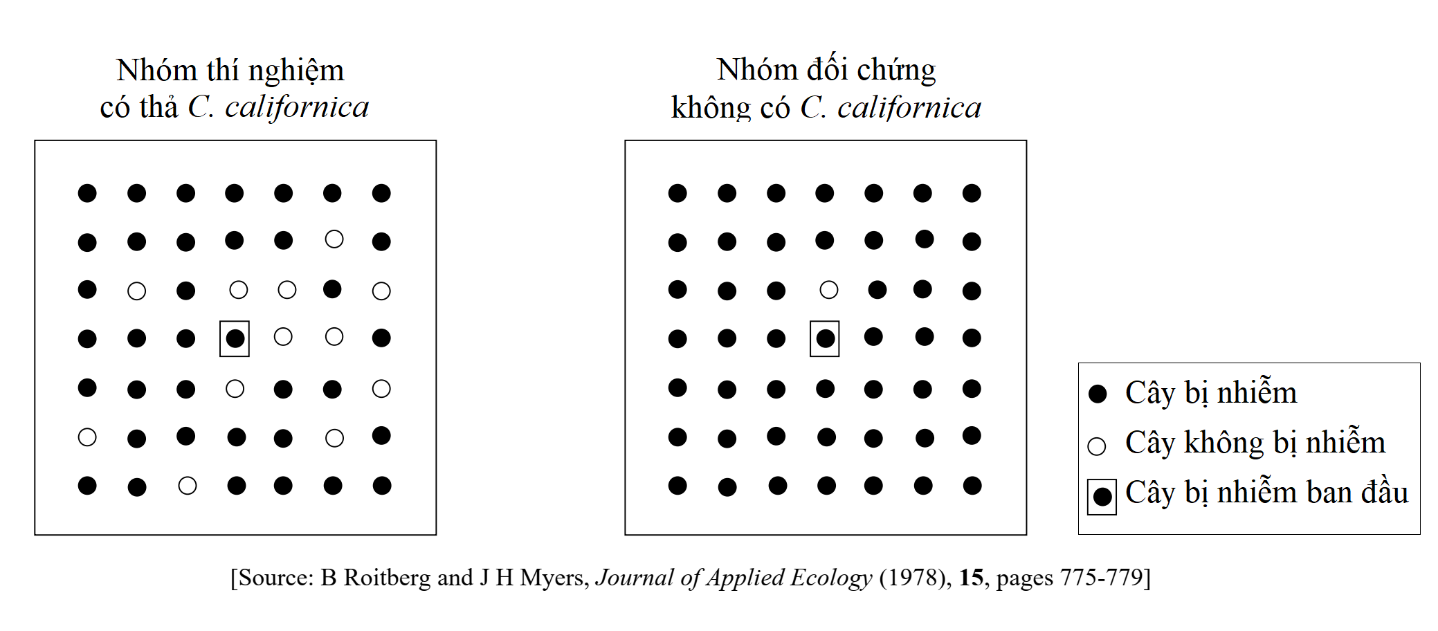
\includegraphics[width=0.73\textwidth]{image/cdle01_image1.png}
\end{center}
\figcaption{1}{Kết quả biểu hiện bệnh của cây đậu ở lô thí nghiệm và lô đối chứng.}

\hfill\textbf{Nguồn: B Roitberg and J H Myers, Journal of Applied Ecology (1978), 15, pages 775-779}
\end{readingpassage}
\vspace{2pt}
\question[Trắc nghiệm]{Mục tiêu chính của nghiên cứu này là gì?}
\par\vspace{4pt}
\noindent\hangindent=2.2em\hangafter=1\choiceitem{A}{Xác định khoảng cách tối ưu giữa các cây đậu để hạn chế sự lây lan của virus đốm vàng lá.}\par\vspace{4pt}
\noindent\hangindent=2.2em\hangafter=1\choiceitem{B}{So sánh hiệu quả kiểm soát rệp đậu của bọ rùa californica với các loài bọ rùa khác.}\par\vspace{4pt}
\noindent\hangindent=2.2em\hangafter=1\choiceitem{C}{Đánh giá tác động của bọ rùa lên khả năng truyền bệnh virus của rệp đậu.}\par\vspace{4pt}
\noindent\hangindent=2.2em\hangafter=1\choiceitem{D}{Đánh giá thời gian cần thiết để virus đốm vàng lá biểu hiện triệu chứng trên cây đậu.}\par\vspace{4pt}
\question[Trắc nghiệm]{Biến số độc lập trong thí nghiệm này là gì?}
\par\vspace{4pt}
\noindent\hangindent=2.2em\hangafter=1\choiceitem{A}{Số lượng cây đậu bị nhiễm bệnh.}\par\vspace{4pt}
\noindent\hangindent=2.2em\hangafter=1\choiceitem{B}{Sự hiện diện hay vắng mặt của bọ rùa.}\par\vspace{4pt}
\noindent\hangindent=2.2em\hangafter=1\choiceitem{C}{Số lượng rệp đậu được đặt lên cây.}\par\vspace{4pt}
\noindent\hangindent=2.2em\hangafter=1\choiceitem{D}{Khoảng cách giữa các cây đậu.}\par\vspace{4pt}
\question[Trắc nghiệm]{Mục đích chính của lô đối chứng là gì?}
\par\vspace{4pt}
\noindent\hangindent=2.2em\hangafter=1\choiceitem{A}{Để chứng minh rằng rệp đậu không gây hại.}\par\vspace{4pt}
\noindent\hangindent=2.2em\hangafter=1\choiceitem{B}{Để cung cấp một mốc so sánh về vai trò bọ rùa.}\par\vspace{4pt}
\noindent\hangindent=2.2em\hangafter=1\choiceitem{C}{Để đảm bảo tất cả các cây đậu đều có khả năng bị nhiễm bệnh.}\par\vspace{4pt}
\noindent\hangindent=2.2em\hangafter=1\choiceitem{D}{Để nuôi bọ rùa cho các thí nghiệm trong tương lai.}\par\vspace{4pt}
\question[Trắc nghiệm]{Việc các nhà khoa học đặt rệp lên cây bị nhiễm và để chúng ăn trong 24 giờ nhằm mục đích gì?}
\par\vspace{4pt}
\noindent\hangindent=2.2em\hangafter=1\choiceitem{A}{Để làm suy yếu cây bị nhiễm ban đầu.}\par\vspace{4pt}
\noindent\hangindent=2.2em\hangafter=1\choiceitem{B}{Để rệp có đủ thời gian mang virus trước khi lây sang các cây khác.}\par\vspace{4pt}
\noindent\hangindent=2.2em\hangafter=1\choiceitem{C}{Để kiểm tra xem bọ rùa có ăn rệp trên cây bị nhiễm hay không.}\par\vspace{4pt}
\noindent\hangindent=2.2em\hangafter=1\choiceitem{D}{Để tính toán tốc độ sinh sản của rệp.}\par\vspace{4pt}
\question[Ghép đôi]{Ghép đôi giữa các thành phần thí nghiệm với vai trò của chúng trong nghiên cứu.}

\vspace{6pt}
\setstretch{1.3}

\textit{Cột B:}
\vspace{-6pt}
\par\vspace{4pt}
\noindent\hangindent=2.2em\hangafter=1\choiceitem{A}{Sinh vật ăn thịt}\par\vspace{4pt}
\noindent\hangindent=2.2em\hangafter=1\choiceitem{B}{Trung gian truyền bệnh}\par\vspace{4pt}
\noindent\hangindent=2.2em\hangafter=1\choiceitem{C}{Sinh vật gây bệnh}\par\vspace{4pt}
\noindent\hangindent=2.2em\hangafter=1\choiceitem{D}{Vật chủ}\par\vspace{4pt}

\vspace{6pt}

\renewcommand{\arraystretch}{1.6}
{\small\setstretch{1.0}
\begin{longtable}{|>{\raggedright\arraybackslash}m{0.44\textwidth}|>{\centering\arraybackslash}m{0.44\textwidth}|}
\hline
\rowcolor{primaryBlue!12}
\multicolumn{1}{|c|}{\cellcolor{primaryBlue!12}\textbf{Cột A}} & \cellcolor{primaryBlue!12}\textbf{Cột B} \\
\hline
\endfirsthead
\hline
\rowcolor{primaryBlue!12}
\multicolumn{1}{|c|}{\cellcolor{primaryBlue!12}\textbf{Cột A}} & \cellcolor{primaryBlue!12}\textbf{Cột B} \\
\hline
\endhead
1. Bọ rùa californica & \dropbox[2.5cm] \\
\hline
2. Rệp đậu & \dropbox[2.5cm] \\
\hline
3. Virus đốm vàng lá & \dropbox[2.5cm] \\
\hline
4. Cây đậu & \dropbox[2.5cm] \\
\hline
\end{longtable}
}
\question[Điền khuyết]{Điền từ/cụm từ thích hợp (không quá 2 tiếng) vào chỗ trống:}

\vspace{5pt}
\setstretch{1.4}
Trong nghiên cứu này, các nhà khoa học thiết kế thí nghiệm để đánh giá tác động của (1)\,\dropbox[2.5cm] đối với khả năng (2)\,\dropbox[2.5cm] của rệp đậu. Họ trồng cây đậu trong (3)\,\dropbox[2cm] với khoảng cách giữa các cây là (4)\,\dropbox[2cm]. Lô thí nghiệm có rệp và bọ rùa, trong khi lô (5)\,\dropbox[2.5cm] chỉ có rệp mà không có bọ rùa. Dữ liệu về biểu hiện bệnh được thu thập sau (6)\,\dropbox[2cm] kể từ khi loại bỏ côn trùng.

\question[Điền khuyết]{Điền số thích hợp (làm tròn đến hàng đơn vị) vào chỗ trống:}

\vspace{5pt}
\setstretch{1.4}
Tổng thời gian của thí nghiệm là (1)\,\dropbox[2cm] ngày. Thời gian rệp đậu có mặt trong thí nghiệm là (2)\,\dropbox[2cm] ngày. Tổng số rệp sử dụng trong nghiên cứu là (3)\,\dropbox[2cm] con. Tổng số bọ rùa là (4)\,\dropbox[2cm] con. Bọ rùa và rệp bị loại bỏ sau ngày thứ (5)\,\dropbox[2cm] của thí nghiệm.

Trong lô thí nghiệm, tổng số cây là (6)\,\dropbox[2cm] cây, ban đầu có (7)\,\dropbox[2cm] cây không mắc bệnh. Khi kết thúc nghiên cứu, số cây nhiễm mới là (8)\,\dropbox[2cm] cây và số cây không nhiễm bệnh là (9)\,\dropbox[2cm] cây. Tỉ lệ mắc bệnh mới của lô thí nghiệm là (10)\,\dropbox[2cm]\,\% so với (11)\,\dropbox[2cm]\,\% ở lô đối chứng.

\question[Đúng/Sai]{Dựa vào kết quả thí nghiệm, hãy xác định những phát biểu sau đây là đúng hay sai:}

\truefalsehead
\truefalseitem{Có sự khác biệt rõ rệt về số liệu giữa lô đối chứng và lô thí nghiệm.}
\truefalseitem{Bọ rùa có khả năng giúp cây đậu có khả năng đề kháng với virus đốm vàng lá.}
\truefalseitem{Bọ rùa có thể tác động làm giảm mức độ lây lan của bệnh đốm vàng lá.}
\truefalseitem{Số lượng bọ rùa tương quan thuận với mức độ lây lan của virus.}
\truefalseend
\question[Trắc nghiệm]{Coi lô thí nghiệm ban đầu là lô 1, lô đối chứng là lô 2, nếu bố trí một lô thứ ba thực hiện thả bọ rùa và rệp cùng lúc thì dựa vào nghiên cứu trên, dự đoán khả năng cao nhất kết quả của lô 3 sẽ như thế nào?}
\par\vspace{4pt}
\noindent\hangindent=2.2em\hangafter=1\choiceitem{A}{Tương tự kết quả lô 1.}\par\vspace{4pt}
\noindent\hangindent=2.2em\hangafter=1\choiceitem{B}{Tương tự kết quả lô 2.}\par\vspace{4pt}
\noindent\hangindent=2.2em\hangafter=1\choiceitem{C}{Số cây bị nhiễm ít hơn lô 1.}\par\vspace{4pt}
\noindent\hangindent=2.2em\hangafter=1\choiceitem{D}{Không dự đoán được.}\par\vspace{4pt}
\question[Trắc nghiệm]{Nếu thí nghiệm này được lặp lại trên một cánh đồng mở thay vì trong nhà kính, yếu tố nào có thể ảnh hưởng nhiều nhất đến kết quả?}
\par\vspace{4pt}
\noindent\hangindent=2.2em\hangafter=1\choiceitem{A}{Sự di cư của bọ rùa và sự xâm nhập của các loài săn mồi khác.}\par\vspace{4pt}
\noindent\hangindent=2.2em\hangafter=1\choiceitem{B}{Gió có thể giúp rệp bay xa hơn.}\par\vspace{4pt}
\noindent\hangindent=2.2em\hangafter=1\choiceitem{C}{Ánh sáng mặt trời tự nhiên sẽ giúp cây khỏe hơn.}\par\vspace{4pt}
\noindent\hangindent=2.2em\hangafter=1\choiceitem{D}{Nhiệt độ thay đổi làm giảm sức sống của rệp.}\par\vspace{4pt}
\question[Trắc nghiệm]{Giả sử ở lô thí nghiệm, côn trùng được để kéo dài thêm 3 ngày nữa (tổng cộng 6 ngày) trước khi loại bỏ. Dự đoán nào là hợp lý nhất cho lô thí nghiệm?}
\par\vspace{4pt}
\noindent\hangindent=2.2em\hangafter=1\choiceitem{A}{Bọ rùa sẽ ăn hết sạch rệp và không có thêm cây nào bị nhiễm bệnh.}\par\vspace{4pt}
\noindent\hangindent=2.2em\hangafter=1\choiceitem{B}{Số cây bị nhiễm bệnh có khả năng sẽ tăng lên một chút so với ban đầu.}\par\vspace{4pt}
\noindent\hangindent=2.2em\hangafter=1\choiceitem{C}{Sẽ có cây bị chết vì rệp hút quá nhiều chất dinh dưỡng.}\par\vspace{4pt}
\noindent\hangindent=2.2em\hangafter=1\choiceitem{D}{Không dự đoán được.}\par\vspace{4pt}
\question[Trắc nghiệm]{Yếu tố nào sau đây làm thí nghiệm không tương tự như mô hình mối quan hệ giữa các sinh vật ở đồng ruộng thực tế?}
\par\vspace{4pt}
\noindent\hangindent=2.2em\hangafter=1\choiceitem{A}{Sử dụng rệp là trung gian truyền bệnh.}\par\vspace{4pt}
\noindent\hangindent=2.2em\hangafter=1\choiceitem{B}{Cho cây mang bệnh trồng cùng với cây không nhiễm bệnh.}\par\vspace{4pt}
\noindent\hangindent=2.2em\hangafter=1\choiceitem{C}{Chủ động thêm và loại bỏ rệp, bọ rùa.}\par\vspace{4pt}
\noindent\hangindent=2.2em\hangafter=1\choiceitem{D}{Chỉ sử dụng virus đốm vàng lá ở đậu.}\par\vspace{4pt}
\question[Trắc nghiệm]{Để tăng độ tin cậy và mở rộng số liệu nghiên cứu về vai trò của bọ rùa, các nhà khoa học nên thay đổi yếu tố nào sau đây? (Chọn nhiều đáp án đúng)}
\par\vspace{4pt}
\noindent\hangindent=2.2em\hangafter=1\choiceitemBox{A}{Tăng số lượng cây đậu trong mỗi lô.}\par\vspace{4pt}
\noindent\hangindent=2.2em\hangafter=1\choiceitemBox{B}{Thay đổi số lượng của rệp.}\par\vspace{4pt}
\noindent\hangindent=2.2em\hangafter=1\choiceitemBox{C}{Thay đổi số lượng của bọ rùa.}\par\vspace{4pt}
\noindent\hangindent=2.2em\hangafter=1\choiceitemBox{D}{Thay đổi thời gian loại bỏ côn trùng.}\par\vspace{4pt}
\noindent\hangindent=2.2em\hangafter=1\choiceitemBox{E}{Thay đổi nhiệt độ môi trường.}\par\vspace{4pt}

% ─────────────────────────────────────────────────────────────
% CHỦ ĐỀ 02: TÁC ĐỘNG CỦA TỪ TRƯỜNG LÊN KHẢ NĂNG ĐỊNH HƯỚNG CỦA BỒ CÂU ĐƯA THƯ (thuộc B.II.1.1)
% ─────────────────────────────────────────────────────────────
\newpage
\setcounter{qcounter}{0}

\phantomsection\label{b1_cd02}
\begin{topicbox}{\large CHỦ ĐỀ 02: TÁC ĐỘNG CỦA TỪ TRƯỜNG LÊN KHẢ NĂNG ĐỊNH HƯỚNG CỦA BỒ CÂU ĐƯA THƯ}
\vspace{8pt}
\textit{Đọc đoạn văn sau và trả lời các câu hỏi.}
\vspace{6pt}
\end{topicbox}
\vspace{5pt}
\begin{readingpassage}[]
\setstretch{1.3}
Bồ câu đưa thư có một khả năng rất đặc biệt: dù bị đưa đi rất xa nơi chúng lớn lên, chúng vẫn có khả năng xác định chính xác đường để bay về nhà. Các nhà khoa học đưa ra giả thuyết rằng: bồ câu non có thể cảm nhận được từ trường của Trái Đất để tìm đường, giống như chúng có một tấm bản đồ vô hình trong đầu vậy.

Để kiểm tra sự tác động của từ trường lên định hướng đường bay của chim bồ câu, họ đã làm thí nghiệm với những chú bồ câu chưa bao giờ rời tổ. Họ chia những chú bồ câu thành 3 nhóm và làm như sau:

\begin{itemize}[leftmargin=*, itemsep=3pt, label=\textcolor{accentBlue}{\textbf{--}}]
\item \textbf{Nhóm 1:} Những chú bồ câu được vận chuyển trong hộp kín đến địa điểm thả và thả ra một cách bình thường.
\item \textbf{Nhóm 2 (Gây nhiễu sau khi đến):} Những chú bồ câu được vận chuyển trong hộp kín đến địa điểm thả. Chỉ sau khi đến nơi, chúng được đặt trong một từ trường nhân tạo bị thay đổi liên tục để gây nhiễu trước khi được thả ra.
\item \textbf{Nhóm 3 (Gây nhiễu trên đường đi):} Bồ câu đặt trong hộp kín và bị tác động bởi từ trường nhân tạo thay đổi liên tục trong suốt cả chuyến đi đến nơi thả. Khi đến nơi, dừng gây nhiễu và thả.
\end{itemize}

Các nhà khoa học ghi lại hướng bay của từng con chim và đếm số lượng của chúng. Kết quả biểu thị ở sơ đồ dưới đây.

\vspace{4pt}
\textit{Cột B:}
\begin{itemize}[leftmargin=*, itemsep=2pt, label=\textcolor{accentBlue}{\textbf{--}}]
\item Tâm vòng tròn: Là nơi họ thả những chú bồ câu.
\item Mỗi chấm đen: Tương ứng với hướng bay của một chú bồ câu.
\item Đường đứt nét (- - -): Là hướng chính xác để bay về nhà.
\item Mũi tên liền: Chỉ hướng bay trung bình của cả đàn.
\end{itemize}

\begin{center}
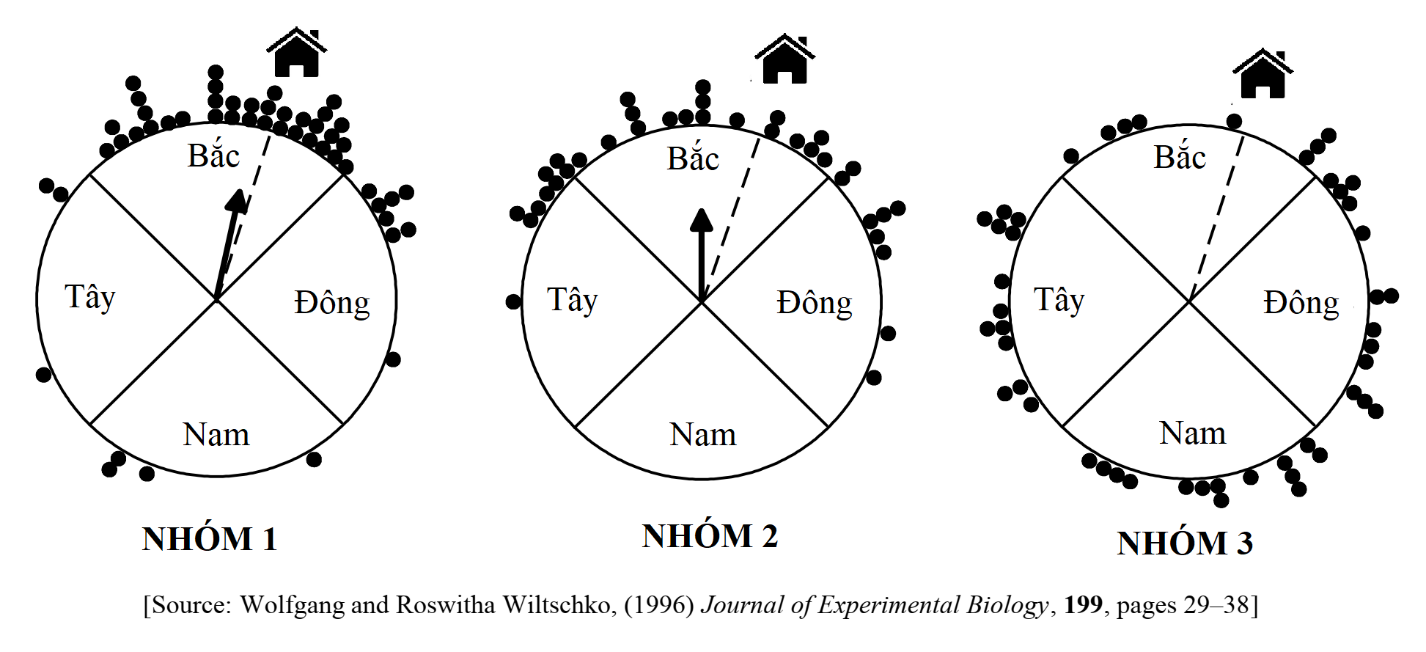
\includegraphics[width=0.73\textwidth]{image/cdle02_image1.png}
\end{center}
\figcaption{1}{Sơ đồ hướng bay của bồ câu trong 3 nhóm thí nghiệm.}

\hfill\textbf{Nguồn: Wolfgang and Roswitha Wiltschko, (1996) Journal of Experimental Biology, 199, pages 29--38}
\end{readingpassage}
\vspace{2pt}
\question[Trắc nghiệm]{Khả năng đặc biệt được quan sát thấy ở bồ câu đưa thư là gì?}
\par\vspace{4pt}
\noindent\hangindent=2.2em\hangafter=1\choiceitem{A}{Khả năng bay với tốc độ cực nhanh để đưa thư kịp thời.}\par\vspace{4pt}
\noindent\hangindent=2.2em\hangafter=1\choiceitem{B}{Khả năng xác định chính xác đường để bay về nhà dù bị đưa đi rất xa.}\par\vspace{4pt}
\noindent\hangindent=2.2em\hangafter=1\choiceitem{C}{Khả năng nhớ đường đi qua nhiều lần bay thử nghiệm trước đó.}\par\vspace{4pt}
\noindent\hangindent=2.2em\hangafter=1\choiceitem{D}{Khả năng giao tiếp với nhau để tìm đường về tổ theo đàn.}\par\vspace{4pt}
\question[Trắc nghiệm]{Theo giả thuyết của các nhà khoa học, yếu tố nào giúp bồ câu định hướng để tìm đường về nhà?}
\par\vspace{4pt}
\noindent\hangindent=2.2em\hangafter=1\choiceitem{A}{Trí nhớ không gian của chúng về vùng lãnh thổ quen thuộc.}\par\vspace{4pt}
\noindent\hangindent=2.2em\hangafter=1\choiceitem{B}{Vị trí mặt trời và các ngôi sao trên bầu trời.}\par\vspace{4pt}
\noindent\hangindent=2.2em\hangafter=1\choiceitem{C}{Từ trường của Trái Đất mà bồ câu có thể cảm nhận được.}\par\vspace{4pt}
\noindent\hangindent=2.2em\hangafter=1\choiceitem{D}{Khứu giác đặc biệt nhạy bén giúp nhận biết mùi quen thuộc.}\par\vspace{4pt}
\question[Trắc nghiệm]{Các nhà khoa học đã chọn loại bồ câu nào để làm thí nghiệm?}
\par\vspace{4pt}
\noindent\hangindent=2.2em\hangafter=1\choiceitem{A}{Bồ câu đã từng đưa thư nhiều lần.}\par\vspace{4pt}
\noindent\hangindent=2.2em\hangafter=1\choiceitem{B}{Bồ câu đã được huấn luyện đặc biệt.}\par\vspace{4pt}
\noindent\hangindent=2.2em\hangafter=1\choiceitem{C}{Bồ câu đã trưởng thành và có kinh nghiệm bay.}\par\vspace{4pt}
\noindent\hangindent=2.2em\hangafter=1\choiceitem{D}{Bồ câu chưa bao giờ rời tổ.}\par\vspace{4pt}
\question[Ghép đôi]{Ghép nhóm nghiên cứu và cách tác động từ trường nhân tạo.}

\vspace{6pt}
\setstretch{1.3}

\textit{Cột B:}
\vspace{-6pt}
\par\vspace{4pt}
\noindent\hangindent=2.2em\hangafter=1\choiceitem{A}{Không tác động}\par\vspace{4pt}
\noindent\hangindent=2.2em\hangafter=1\choiceitem{B}{Tác động trên đường đi đến địa điểm thả}\par\vspace{4pt}
\noindent\hangindent=2.2em\hangafter=1\choiceitem{C}{Tác động khi đã đến địa điểm thả}\par\vspace{4pt}

\vspace{6pt}

\renewcommand{\arraystretch}{1.6}
{\small\setstretch{1.0}
\begin{longtable}{|>{\raggedright\arraybackslash}m{0.44\textwidth}|>{\centering\arraybackslash}m{0.44\textwidth}|}
\hline
\rowcolor{primaryBlue!12}
\multicolumn{1}{|c|}{\cellcolor{primaryBlue!12}\textbf{Cột A}} & \cellcolor{primaryBlue!12}\textbf{Cột B} \\
\hline
\endfirsthead
\hline
\rowcolor{primaryBlue!12}
\multicolumn{1}{|c|}{\cellcolor{primaryBlue!12}\textbf{Cột A}} & \cellcolor{primaryBlue!12}\textbf{Cột B} \\
\hline
\endhead
1. Nhóm 1 & \dropbox[2.5cm] \\
\hline
2. Nhóm 2 & \dropbox[2.5cm] \\
\hline
3. Nhóm 3 & \dropbox[2.5cm] \\
\hline
\end{longtable}
}
\question[Ghép đôi]{Ghép đôi giữa các yếu tố thí nghiệm với vai trò của chúng.}

\vspace{6pt}
\setstretch{1.3}

\textit{Cột B:}
\vspace{-6pt}
\par\vspace{4pt}
\noindent\hangindent=2.2em\hangafter=1\choiceitem{A}{Nhóm đối chứng}\par\vspace{4pt}
\noindent\hangindent=2.2em\hangafter=1\choiceitem{B}{Biến số độc lập}\par\vspace{4pt}
\noindent\hangindent=2.2em\hangafter=1\choiceitem{C}{Biến số phụ thuộc}\par\vspace{4pt}
\noindent\hangindent=2.2em\hangafter=1\choiceitem{D}{Yếu tố kiểm soát}\par\vspace{4pt}

\vspace{6pt}

\renewcommand{\arraystretch}{1.6}
{\small\setstretch{1.0}
\begin{longtable}{|>{\raggedright\arraybackslash}m{0.44\textwidth}|>{\centering\arraybackslash}m{0.44\textwidth}|}
\hline
\rowcolor{primaryBlue!12}
\multicolumn{1}{|c|}{\cellcolor{primaryBlue!12}\textbf{Cột A}} & \cellcolor{primaryBlue!12}\textbf{Cột B} \\
\hline
\endfirsthead
\hline
\rowcolor{primaryBlue!12}
\multicolumn{1}{|c|}{\cellcolor{primaryBlue!12}\textbf{Cột A}} & \cellcolor{primaryBlue!12}\textbf{Cột B} \\
\hline
\endhead
1. Nhóm 1 & \dropbox[2.5cm] \\
\hline
2. Phương pháp gây nhiễu & \dropbox[2.5cm] \\
\hline
3. Hướng bay của chim & \dropbox[2.5cm] \\
\hline
4. Địa điểm thả chim & \dropbox[2.5cm] \\
\hline
\end{longtable}
}
\question[Trắc nghiệm]{Trong sơ đồ thể hiện kết quả thí nghiệm, mũi tên liền thể hiện điều gì?}
\par\vspace{4pt}
\noindent\hangindent=2.2em\hangafter=1\choiceitem{A}{Đường bay chính xác để về nhà.}\par\vspace{4pt}
\noindent\hangindent=2.2em\hangafter=1\choiceitem{B}{Hướng bay của bồ câu nhanh nhất.}\par\vspace{4pt}
\noindent\hangindent=2.2em\hangafter=1\choiceitem{C}{Hướng bay trung bình của cả đàn.}\par\vspace{4pt}
\noindent\hangindent=2.2em\hangafter=1\choiceitem{D}{Vị trí nơi bồ câu được thả ra.}\par\vspace{4pt}
\question[Trắc nghiệm]{Những thông tin nào được thể hiện trong sơ đồ kết quả thí nghiệm? (Chọn nhiều đáp án đúng)}
\par\vspace{4pt}
\noindent\hangindent=2.2em\hangafter=1\choiceitemBox{A}{Nơi thả những chú bồ câu.}\par\vspace{4pt}
\noindent\hangindent=2.2em\hangafter=1\choiceitemBox{B}{Thời gian bay của từng con bồ câu.}\par\vspace{4pt}
\noindent\hangindent=2.2em\hangafter=1\choiceitemBox{C}{Hướng bay của từng chú bồ câu.}\par\vspace{4pt}
\noindent\hangindent=2.2em\hangafter=1\choiceitemBox{D}{Cường độ từ trường tại điểm thả.}\par\vspace{4pt}
\noindent\hangindent=2.2em\hangafter=1\choiceitemBox{E}{Hướng chính xác để bay về nhà.}\par\vspace{4pt}
\noindent\hangindent=2.2em\hangafter=1\choiceitemBox{F}{Hướng bay trung bình của cả đàn.}\par\vspace{4pt}
\question[Đúng/Sai]{Dựa vào bài đọc, hãy xác định những phát biểu sau đây là đúng hay sai khi nói về thí nghiệm với bồ câu đưa thư:}

\truefalsehead
\truefalseitem{Cả ba nhóm bồ câu đều bị gây nhiễu từ trường ở một giai đoạn nào đó.}
\truefalseitem{Các nhà khoa học quan sát hướng bay của bồ câu sau khi thả.}
\truefalseitem{Bồ câu trong thí nghiệm đều là những con đã có kinh nghiệm bay trước đó.}
\truefalseitem{Nhóm 1 được vận chuyển và thả trong điều kiện từ trường tự nhiên.}
\truefalseitem{Nhóm 3 ngừng bị gây nhiễu từ trường khi đến nơi thả.}
\truefalseend
\question[Trắc nghiệm]{Dựa vào sơ đồ, hướng bay của nhóm nào thể hiện sự mất phương hướng rõ rệt nhất, với các cá thể phân tán gần như ngẫu nhiên?}
\par\vspace{4pt}
\noindent\choiceitem{A}{Nhóm 1.}\hspace{2em}\choiceitem{B}{Nhóm 2.}\hspace{2em}\choiceitem{C}{Nhóm 3.}\par\vspace{4pt}
\question[Trắc nghiệm]{Tại sao biểu đồ nhóm 3 không có mũi tên?}
\par\vspace{4pt}
\noindent\hangindent=2.2em\hangafter=1\choiceitem{A}{Đây là lỗi kỹ thuật trong cách trình bày kết quả thí nghiệm.}\par\vspace{4pt}
\noindent\hangindent=2.2em\hangafter=1\choiceitem{B}{Các bồ câu nhóm 3 không bay đi sau khi được thả ra.}\par\vspace{4pt}
\noindent\hangindent=2.2em\hangafter=1\choiceitem{C}{Hướng bay phân tán dẫn đến không tổ hợp được mũi tên trung bình.}\par\vspace{4pt}
\noindent\hangindent=2.2em\hangafter=1\choiceitem{D}{Nhóm 3 không đủ số lượng bồ câu để tính hướng bay trung bình.}\par\vspace{4pt}
\noindent\hangindent=2.2em\hangafter=1\choiceitem{E}{Mũi tên của nhóm 3 trùng với đường đứt nét nên không hiển thị riêng.}\par\vspace{4pt}
\question[Trắc nghiệm]{Vắng mặt của mũi tên trong biểu đồ nhóm 3 cung cấp bằng chứng cho giả thuyết nào về cơ chế định hướng của bồ câu?}
\par\vspace{4pt}
\noindent\hangindent=2.2em\hangafter=1\choiceitem{A}{Bồ câu chủ yếu sử dụng thị giác để định hướng.}\par\vspace{4pt}
\noindent\hangindent=2.2em\hangafter=1\choiceitem{B}{Bồ câu lưu trữ thông tin từ trường tại tổ trước khi bay đi.}\par\vspace{4pt}
\noindent\hangindent=2.2em\hangafter=1\choiceitem{C}{Bồ câu sử dụng vị trí mặt trời để định hướng.}\par\vspace{4pt}
\noindent\hangindent=2.2em\hangafter=1\choiceitem{D}{Bồ câu thu thập và lưu trữ thông tin từ trường trong quá trình di chuyển.}\par\vspace{4pt}
\noindent\hangindent=2.2em\hangafter=1\choiceitem{E}{Bồ câu phụ thuộc chủ yếu vào trí nhớ không gian để tìm đường về.}\par\vspace{4pt}
\question[Đúng/Sai]{Các phát biểu sau đây đúng hay sai khi nói về kết quả của thí nghiệm:}

\truefalsehead
\truefalseitem{Các con chim bồ câu có thể có cảm nhận từ trường không giống nhau.}
\truefalseitem{Tỉ lệ bồ câu bay về hướng tổ là nhiều nhất.}
\truefalseitem{Những con chim bồ câu bay lệch hướng tổ là những cá thể không có khả năng cảm nhận từ trường.}
\truefalseitem{Chim bay theo nhiều hướng phủ nhận giả thuyết ảnh hưởng của từ trường lên định hướng đường bay của chim bồ câu.}
\truefalseend
\question[Trắc nghiệm]{Vai trò của việc sử dụng bồ câu ``chưa bao giờ rời tổ'' trong thí nghiệm này là gì? (Chọn nhiều đáp án đúng)}
\par\vspace{4pt}
\noindent\hangindent=2.2em\hangafter=1\choiceitemBox{A}{Để đảm bảo rằng chúng không có kinh nghiệm bay trước đó.}\par\vspace{4pt}
\noindent\hangindent=2.2em\hangafter=1\choiceitemBox{B}{Để loại trừ khả năng chúng định hướng dựa trên trí nhớ không gian.}\par\vspace{4pt}
\noindent\hangindent=2.2em\hangafter=1\choiceitemBox{C}{Để chứng minh khả năng định hướng là bẩm sinh, không cần học tập.}\par\vspace{4pt}
\noindent\hangindent=2.2em\hangafter=1\choiceitemBox{D}{Để tránh sự tác động của các yếu tố nhiệt độ, hướng chiếu sáng.}\par\vspace{4pt}
\question[Trắc nghiệm]{Dựa vào kết quả thí nghiệm, xếp hạng độ chính xác định hướng của các nhóm từ cao đến thấp:}
\par\vspace{4pt}
\noindent\hangindent=2.2em\hangafter=1\choiceitem{A}{Nhóm 1 > Nhóm 2 > Nhóm 3.}\par\vspace{4pt}
\noindent\hangindent=2.2em\hangafter=1\choiceitem{B}{Nhóm 2 > Nhóm 1 > Nhóm 3.}\par\vspace{4pt}
\noindent\hangindent=2.2em\hangafter=1\choiceitem{C}{Nhóm 3 > Nhóm 2 > Nhóm 1.}\par\vspace{4pt}
\noindent\hangindent=2.2em\hangafter=1\choiceitem{D}{Nhóm 1 > Nhóm 3 > Nhóm 2.}\par\vspace{4pt}
\question[Trắc nghiệm]{Từ kết quả thí nghiệm, có thể rút ra kết luận nào về cơ chế cảm nhận từ trường của bồ câu? (Chọn nhiều đáp án đúng)}
\par\vspace{4pt}
\noindent\hangindent=2.2em\hangafter=1\choiceitemBox{A}{Bồ câu có thể phát hiện sự thay đổi của từ trường theo thời gian.}\par\vspace{4pt}
\noindent\hangindent=2.2em\hangafter=1\choiceitemBox{B}{Bồ câu có các tế bào thần kinh chuyên biệt để cảm nhận từ trường.}\par\vspace{4pt}
\noindent\hangindent=2.2em\hangafter=1\choiceitemBox{C}{Cơ chế cảm nhận từ trường của bồ câu có thể hoạt động độc lập với thị giác.}\par\vspace{4pt}
\noindent\hangindent=2.2em\hangafter=1\choiceitemBox{D}{Bồ câu có thể phân biệt giữa từ trường tự nhiên và từ trường nhân tạo.}\par\vspace{4pt}
\noindent\hangindent=2.2em\hangafter=1\choiceitemBox{E}{Khả năng cảm nhận từ trường của bồ câu suy giảm theo tuổi tác.}\par\vspace{4pt}
\noindent\hangindent=2.2em\hangafter=1\choiceitemBox{F}{Đây là tập tính bẩm sinh nhưng thể hiện không đồng đều giữa các cá thể.}\par\vspace{4pt}
\question[Trắc nghiệm]{Thí nghiệm về khả năng định hướng của bồ câu còn tồn tại những nhược điểm nào trong bố trí? (Chọn nhiều đáp án đúng)}
\par\vspace{4pt}
\noindent\hangindent=2.2em\hangafter=1\choiceitemBox{A}{Số lượng cá thể sử dụng trong mỗi nhóm là không bằng nhau.}\par\vspace{4pt}
\noindent\hangindent=2.2em\hangafter=1\choiceitemBox{B}{Không cung cấp thông tin về cường độ và tần số của từ trường nhân tạo được sử dụng để gây nhiễu.}\par\vspace{4pt}
\noindent\hangindent=2.2em\hangafter=1\choiceitemBox{C}{Không giải thích liệu các yếu tố môi trường khác (như điều kiện thời tiết, gió, ánh sáng) có được kiểm soát hay không.}\par\vspace{4pt}
\noindent\hangindent=2.2em\hangafter=1\choiceitemBox{D}{Không nêu rõ khoảng cách từ điểm thả đến vị trí tổ của bồ câu.}\par\vspace{4pt}
\question[Trắc nghiệm]{Dựa vào kết quả thí nghiệm, dự đoán hợp lý về hướng bay của bồ câu trong trường hợp chúng bị gây nhiễu từ trường cả trong quá trình di chuyển và sau khi đến nơi thả là:}
\par\vspace{4pt}
\noindent\hangindent=2.2em\hangafter=1\choiceitem{A}{Chúng sẽ bay theo hướng hoàn toàn ngẫu nhiên.}\par\vspace{4pt}
\noindent\hangindent=2.2em\hangafter=1\choiceitem{B}{Chúng sẽ bay ngược với hướng về nhà.}\par\vspace{4pt}
\noindent\hangindent=2.2em\hangafter=1\choiceitem{C}{Chúng sẽ bay theo hướng giống nhóm 2 trong thí nghiệm.}\par\vspace{4pt}
\noindent\hangindent=2.2em\hangafter=1\choiceitem{D}{Chúng sẽ bay theo hướng giống nhóm 3 trong thí nghiệm.}\par\vspace{4pt}
\question[Trắc nghiệm]{Nếu gây nhiễu bằng từ trường nhân tạo tại tổ chim trong một khoảng thời gian, sau đó dừng lại. Sau đó thực hiện quá trình vận chuyển và thả chim không tác động từ trường. Từ kết quả nghiên cứu, có thể dự đoán chim bồ câu sẽ có mô hình bay giống nhóm nào sau đây?}
\par\vspace{4pt}
\noindent\choiceitem{A}{Nhóm 1.}\hspace{2em}\choiceitem{B}{Nhóm 2.}\hspace{2em}\choiceitem{C}{Nhóm 3.}\par\vspace{4pt}
\question[Trắc nghiệm]{Nếu kết quả cho thấy tất cả các nhóm đều có hướng bay ngẫu nhiên như nhau, điều này sẽ có nghĩa gì?}
\par\vspace{4pt}
\noindent\hangindent=2.2em\hangafter=1\choiceitem{A}{Giả thuyết về từ trường là đúng.}\par\vspace{4pt}
\noindent\hangindent=2.2em\hangafter=1\choiceitem{B}{Giả thuyết về từ trường bị bác bỏ.}\par\vspace{4pt}
\noindent\hangindent=2.2em\hangafter=1\choiceitem{C}{Cần thực hiện thêm thí nghiệm.}\par\vspace{4pt}
\noindent\hangindent=2.2em\hangafter=1\choiceitem{D}{Chim bồ câu không có khả năng định hướng.}\par\vspace{4pt}

% ─────────────────────────────────────────────────────────────
% CHỦ ĐỀ 03: KHẢ NĂNG HỌC LIÊN KẾT MÀU SẮC VỚI MÙI HƯƠNG Ở ONG MẬT (thuộc B.II.1.1)
% ─────────────────────────────────────────────────────────────
\newpage
\setcounter{qcounter}{0}

\phantomsection\label{b1_cd03}
\begin{topicbox}{\large CHỦ ĐỀ 03: KHẢ NĂNG HỌC LIÊN KẾT MÀU SẮC VỚI MÙI HƯƠNG Ở ONG MẬT}
\vspace{8pt}
\textit{Đọc đoạn văn sau và trả lời các câu hỏi.}
\vspace{6pt}
\end{topicbox}
\vspace{5pt}
\begin{readingpassage}[]
\setstretch{1.3}
Một nghiên cứu được thực hiện để đánh giá xem ong mật (\textit{Apis mellifera}) có thể học cách liên kết một màu sắc với một mùi hương hay không. Thiết bị của thí nghiệm được mô tả ở Hình 1.

\begin{center}
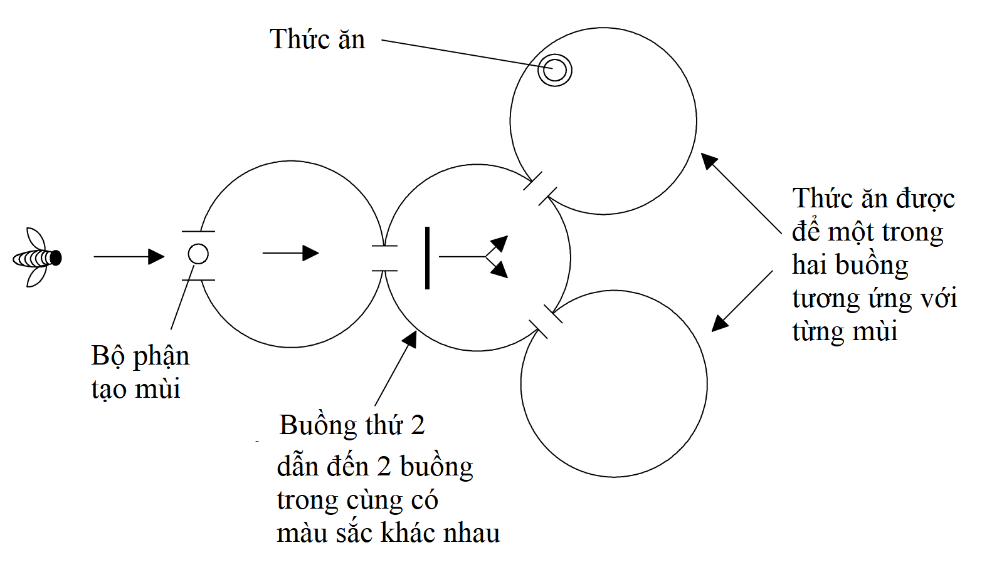
\includegraphics[width=0.55\textwidth]{image/cdle03_image1.png}
\end{center}
\figcaption{1}{Mô hình bố trí thí nghiệm đánh giá khả năng liên kết thông tin thị giác và khứu giác ở ong mật.}

Khi ong bay vào buồng đầu tiên, chúng đi qua một hộp đựng tỏa ra mùi chanh hoặc mùi xoài. Khi ong bay vào buồng thứ hai, không sơn màu, không có mùi hương, có một tấm chắn phía sau đường vào buồng 2 để ngăn ong nhìn thấy buồng trong cùng. Mỗi buồng trong cùng sơn một màu khác nhau (một buồng sơn màu vàng và một buồng sơn màu xanh lam). Một trong hai buồng trong cùng chứa thức ăn, việc để thức ăn ở buồng nào phụ thuộc vào loại mùi xoài hay chanh tỏa ra từ bộ phận tạo mùi ở buồng đầu tiên. Khi mùi hương là chanh, buồng có thức ăn được để ở buồng màu xanh lam. Khi mùi hương là xoài, thức ăn được để ở buồng màu vàng.

Cứ mười phút một lần sẽ thay đổi mùi ở buồng đầu tiên (đồng thời với đó là di chuyển thức ăn tương ứng ở buồng trong cùng). Quy trình này được thực hiện trong hai ngày. Trong ngày đầu tiên của thí nghiệm, trong mỗi lần thả ong vào buồng, ong được phép di chuyển cho đến khi tìm thấy thức ăn. Sau khi tìm thấy thức ăn ong được bắt ra khỏi buồng và lặp lại quá trình. Quá trình ghi số liệu chỉ bắt đầu vào ngày thứ 2, khác với ngày 1, sự lựa chọn đầu tiên của ong được ghi lại và ong được bắt ra khỏi buồng. Kết quả được thể hiện ở biểu đồ dưới đây:

\begin{center}
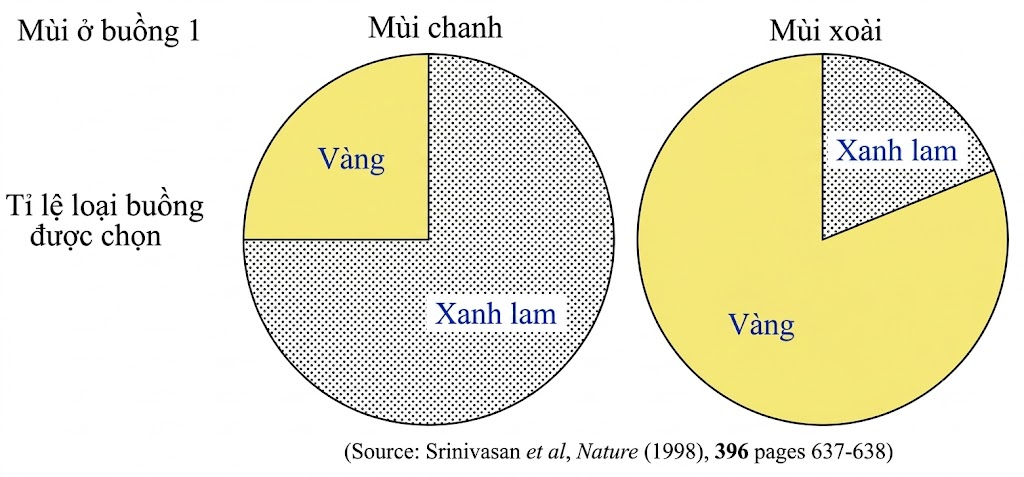
\includegraphics[width=0.55\textwidth]{image/cdle03_image2.png}
\end{center}
\figcaption{2}{Tỉ lệ loại buồng trong cùng mà ong chọn tương ứng với loại mùi mà nó ngửi được ở buồng đầu tiên.}

\hfill\textbf{Nguồn: Srinivasan et al, Nature (1998)}
\end{readingpassage}
\vspace{2pt}
\question[Trắc nghiệm]{Đâu là mục đích chính của thí nghiệm được mô tả trong bài đọc?}
\par\vspace{4pt}
\noindent\hangindent=2.2em\hangafter=1\choiceitem{A}{Xác định loại mùi hương mà ong mật ưa thích nhất trong tự nhiên.}\par\vspace{4pt}
\noindent\hangindent=2.2em\hangafter=1\choiceitem{B}{Kiểm tra khả năng phân biệt màu sắc của ong mật trong điều kiện ánh sáng khác nhau.}\par\vspace{4pt}
\noindent\hangindent=2.2em\hangafter=1\choiceitem{C}{Đánh giá khả năng học liên kết giữa mùi hương và màu sắc của ong mật.}\par\vspace{4pt}
\noindent\hangindent=2.2em\hangafter=1\choiceitem{D}{Khảo sát tốc độ di chuyển của ong mật giữa các buồng thí nghiệm.}\par\vspace{4pt}
\question[Đúng/Sai]{Dựa vào thông tin về thiết kế thí nghiệm, hãy cho biết những phát biểu nào sau đây là đúng hay sai:}

\truefalsehead
\truefalseitem{Bộ phận tạo mùi được bố trí ở buồng đầu tiên.}
\truefalseitem{Mùi hương thay đổi 10 phút một lần.}
\truefalseitem{Buồng thứ 2 có màu vàng hoặc màu xanh lam.}
\truefalseitem{Vị trí của thức ăn không thay đổi trong suốt quá trình thí nghiệm.}
\truefalseitem{Sử dụng 2 loại thức ăn tương ứng với hai loại mùi khác nhau.}
\truefalseitem{Thiết kế thí nghiệm cho phép ong tự do lựa chọn đường đi.}
\truefalseitem{Một con ong chỉ được sử dụng 1 lần trong thí nghiệm.}
\truefalseend
\question[Trắc nghiệm]{Thông số nào sau đây là biến số độc lập trong thí nghiệm?}
\par\vspace{4pt}
\noindent\hangindent=2.2em\hangafter=1\choiceitem{A}{Loại mùi hương ở buồng đầu tiên.}\par\vspace{4pt}
\noindent\hangindent=2.2em\hangafter=1\choiceitem{B}{Màu sắc ở buồng thứ hai.}\par\vspace{4pt}
\noindent\hangindent=2.2em\hangafter=1\choiceitem{C}{Thời gian thay đổi mùi hương.}\par\vspace{4pt}
\noindent\hangindent=2.2em\hangafter=1\choiceitem{D}{Vị trí đặt thức ăn ở buồng trong cùng.}\par\vspace{4pt}
\noindent\hangindent=2.2em\hangafter=1\choiceitem{E}{Loài ong được sử dụng trong thí nghiệm.}\par\vspace{4pt}
\noindent\hangindent=2.2em\hangafter=1\choiceitem{F}{Số lượng ong tham gia vào thí nghiệm.}\par\vspace{4pt}
\question[Trắc nghiệm]{Thông số nào sau đây là biến số phụ thuộc trong thí nghiệm?}
\par\vspace{4pt}
\noindent\hangindent=2.2em\hangafter=1\choiceitem{A}{Loại mùi hương ở buồng đầu tiên.}\par\vspace{4pt}
\noindent\hangindent=2.2em\hangafter=1\choiceitem{B}{Loại buồng cuối cùng được ong lựa chọn.}\par\vspace{4pt}
\noindent\hangindent=2.2em\hangafter=1\choiceitem{C}{Thời gian thay đổi mùi hương.}\par\vspace{4pt}
\noindent\hangindent=2.2em\hangafter=1\choiceitem{D}{Thời gian di chuyển của ong từ buồng 1 đến buồng cuối cùng.}\par\vspace{4pt}
\noindent\hangindent=2.2em\hangafter=1\choiceitem{E}{Loài ong được sử dụng trong thí nghiệm.}\par\vspace{4pt}
\noindent\hangindent=2.2em\hangafter=1\choiceitem{F}{Số lượng ong tham gia vào thí nghiệm.}\par\vspace{4pt}
\question[Trắc nghiệm]{Tấm chắn sau cửa buồng 2 có tác dụng gì?}
\par\vspace{4pt}
\noindent\hangindent=2.2em\hangafter=1\choiceitem{A}{Ngăn ong bay thẳng vào bên trong.}\par\vspace{4pt}
\noindent\hangindent=2.2em\hangafter=1\choiceitem{B}{Ngăn mùi hương bay vào bên trong.}\par\vspace{4pt}
\noindent\hangindent=2.2em\hangafter=1\choiceitem{C}{Ngăn ong nhìn thấy màu sắc của buồng 2.}\par\vspace{4pt}
\noindent\hangindent=2.2em\hangafter=1\choiceitem{D}{Để ong di chuyển tuần tự theo hàng.}\par\vspace{4pt}
\question[Trắc nghiệm]{Thí nghiệm về ong mật chỉ ghi lại dữ liệu vào ngày thứ hai, mục đích của ngày thứ nhất là gì?}
\par\vspace{4pt}
\noindent\hangindent=2.2em\hangafter=1\choiceitem{A}{Tập cho ong quen đường.}\par\vspace{4pt}
\noindent\hangindent=2.2em\hangafter=1\choiceitem{B}{Loại bỏ những con ong chọn sai.}\par\vspace{4pt}
\noindent\hangindent=2.2em\hangafter=1\choiceitem{C}{Ong học tập và tạo kết nối.}\par\vspace{4pt}
\noindent\hangindent=2.2em\hangafter=1\choiceitem{D}{Tìm sai sót của thí nghiệm.}\par\vspace{4pt}
\question[Trắc nghiệm]{Sự khác biệt lớn nhất của cách thực hiện thí nghiệm của ngày 2 so với ngày 1 là gì?}
\par\vspace{4pt}
\noindent\hangindent=2.2em\hangafter=1\choiceitem{A}{Chỉ sử dụng 1 loại mùi hương.}\par\vspace{4pt}
\noindent\hangindent=2.2em\hangafter=1\choiceitem{B}{Chỉ để thức ăn ở 1 buồng cố định.}\par\vspace{4pt}
\noindent\hangindent=2.2em\hangafter=1\choiceitem{C}{Thay đổi màu sắc của các buồng cuối cùng.}\par\vspace{4pt}
\noindent\hangindent=2.2em\hangafter=1\choiceitem{D}{Bị bắt ngay sau khi bò vào buồng cuối cùng.}\par\vspace{4pt}
\question[Đúng/Sai]{Dựa vào dữ liệu từ biểu đồ kết quả, những phát biểu nào sau đây là đúng hay sai:}

\truefalsehead
\truefalseitem{Trên 70\% số ong chọn đúng buồng có thức ăn tương ứng với loại mùi ban đầu.}
\truefalseitem{Mùi xoài có sự kết nối thông tin hiệu quả hơn mùi chanh.}
\truefalseitem{Dữ liệu chưa đủ thuyết phục để kết luận mối liên hệ giữa mùi hương và màu sắc.}
\truefalseitem{Ong có thể phân biệt được mùi xoài với mùi chanh, màu vàng với màu xanh lam.}
\truefalseitem{Ong mật có thể học liên kết hai mùi hương với 2 màu sắc tương ứng.}
\truefalseitem{Ong mật có thể duy trì khả năng nhớ liên kết đã học trong vài tuần mà không cần củng cố.}
\truefalseitem{Ong mật có thể truyền đạt thông tin về liên kết đã học cho các ong khác trong đàn.}
\truefalseend
\question[Trắc nghiệm]{Trong trường hợp mùi chanh, giả sử có 100 con ong tham gia kiểm tra, theo số liệu thống kê thì ước lượng số ong chọn buồng màu vàng là bao nhiêu?}
\par\vspace{4pt}
\noindent\choiceitem{A}{14 con.}\hfill\choiceitem{B}{24 con.}\hfill\choiceitem{C}{34 con.}\hfill\choiceitem{D}{44 con.}
\question[Trắc nghiệm]{Một học sinh cho rằng ``Nếu ong không nhận diện được chanh, lúc đó khi gặp mùi chanh ong sẽ hiểu trường hợp đó là không có mùi và kết nối không mùi với màu xanh lam. Hoặc có thể do chính mùi thức ăn tỏa ra dẫn dụ ong chứ không liên quan đến liên kết màu mùi.'' Để chứng minh là ong có cảm thấy mùi chanh và từ đó có mối liên hệ với màu sắc hay không thì bố trí thí nghiệm nào sau đây vào ngày thứ 3 là hợp lý?}
\par\vspace{4pt}
\noindent\hangindent=2.2em\hangafter=1\choiceitem{A}{Thêm nhóm không mùi, không có thức ăn ở hai buồng cuối.}\par\vspace{4pt}
\noindent\hangindent=2.2em\hangafter=1\choiceitem{B}{Thêm nhóm không mùi, thức ăn cố định ở buồng xanh lam.}\par\vspace{4pt}
\noindent\hangindent=2.2em\hangafter=1\choiceitem{C}{Thêm nhóm không mùi, thức ăn cố định ở buồng màu vàng.}\par\vspace{4pt}
\noindent\hangindent=2.2em\hangafter=1\choiceitem{D}{Thêm nhóm không mùi, thức ăn ngẫu nhiên ở buồng cuối.}\par\vspace{4pt}

% ─────────────────────────────────────────────────────────────
% CHỦ ĐỀ 04: UVB (thuộc B.II.1.1)
% ─────────────────────────────────────────────────────────────
\newpage
\setcounter{qcounter}{0}

\phantomsection\label{b1_cd04}
\begin{topicbox}{\large CHỦ ĐỀ 04: UVB}
\vspace{8pt}
\textit{Đọc đoạn văn sau và trả lời các câu hỏi.}
\vspace{6pt}
\end{topicbox}
\vspace{5pt}
\begin{readingpassage}[]
\setstretch{1.3}
Mặt trời là nguồn phát ra nhiều bước sóng bức xạ tới trái đất. Bầu khí quyển của trái đất hấp thụ một số bước sóng này, trong khi những bước sóng khác thì có khả năng xâm nhập và tiếp cận bề mặt hành tinh. Bức xạ cực tím từ mặt trời có ba loại khác nhau dựa trên bước sóng và khả năng xuyên thấu: UVA, UVB và UVC.

Bức xạ UVB có bước sóng từ 280 đến 320\,nm và một phần được tầng ozon của trái đất hấp thụ. Các tia UVB chạm tới bề mặt có thể được da người hấp thụ và là nguyên nhân gây cháy nắng và nhiều dạng ung thư da. Nhiều sản phẩm, từ kính mắt đến kem chống nắng, được tạo ra để giúp bảo vệ con người khỏi bức xạ UVB. Hai nhóm sinh viên bắt đầu kiểm tra khả năng chặn ánh sáng UVB của vật liệu bằng cách sử dụng máy tính và một cảm biến được thiết kế đặc biệt để phát hiện bức xạ UVB.

\textbf{Nhóm 1:} Các thành viên của Nhóm 1 đặt cảm biến dưới ánh nắng đầy đủ và che chắn cảm biến với nhiều loại kính râm được tuyên bố là có khả năng chống tia UVB. Việc đo lường chỉ số UVB được thực hiện trên cảm biến UVB cho từng sản phẩm và dữ liệu được ghi trong Bảng 1.

\tablecaption{1}{Số liệu phần trăm che chắn tia UVB của các loại kính râm.}
\renewcommand{\arraystretch}{1.3}
{\footnotesize
\setstretch{1.0}%
\begin{center}
\begin{tabular}{|l|c|c|c|c|}
\hline
\rowcolor{primaryBlue!12}
\textbf{Kính} & \textbf{Giá (\$)} & \textbf{UVB trước (mW/m\textsuperscript{2})} & \textbf{UVB sau (mW/m\textsuperscript{2})} & \textbf{Che chắn (\%)} \\
\hline
Cặp A & 10 & 742,3 & 2,7 & 99,6 \\
\hline
Cặp B & 350 & 742,3 & 3,2 & 99,6 \\
\hline
Cặp C & 10 & 742,3 & 4,2 & 99,4 \\
\hline
Cặp D & 25 & 742,3 & 3,5 & 99,5 \\
\hline
Cặp E & 90 & 742,3 & 2,1 & 99,7 \\
\hline
Nhựa trong suốt & N/A & 742,3 & 423,1 & 43,0 \\
\hline
\end{tabular}
\end{center}
}

\vspace{6pt}
\textbf{Nhóm 2:} Các thành viên của Nhóm 2 đặt cảm biến dưới ánh nắng mặt trời và che chắn cảm biến đó bằng một mảnh thủy tinh. Họ đã thử nghiệm các loại kem chống nắng có chỉ số SPF tăng dần (chỉ số đo lường khả năng chống lại tia UV) trên kính và số liệu được ghi trong Bảng 2.

\tablecaption{2}{Chỉ số che chắn UVB của các loại kem chống nắng khác nhau.}
\renewcommand{\arraystretch}{1.3}
{\footnotesize
\setstretch{1.0}%
\begin{center}
\begin{tabular}{|l|c|c|c|c|}
\hline
\rowcolor{primaryBlue!12}
\textbf{Mô tả} & \textbf{SPF} & \textbf{UVB có kem (mW/m\textsuperscript{2})} & \textbf{UVB không kem (mW/m\textsuperscript{2})} & \textbf{Giá (\$)} \\
\hline
Da sẫm màu & 4 & 72,1 & 742,3 & 8,99 \\
\hline
Không thấm nước & 8 & 35,6 & 742,3 & 4,99 \\
\hline
Thể thao & 15 & 20,2 & 742,3 & 7,99 \\
\hline
Kiềm dầu & 30 & 19,8 & 742,3 & 15,99 \\
\hline
Trẻ con & 50 & 18,5 & 742,3 & 10,99 \\
\hline
\end{tabular}
\end{center}
}

\hfill\textbf{Nguồn: ACT -- American College Testing}
\end{readingpassage}
\vspace{2pt}
\question[Trắc nghiệm]{Trong thí nghiệm của Nhóm 1, yếu tố nào sau đây là biến độc lập?}
\par\vspace{4pt}
\noindent\choiceitem{A}{Cường độ ánh sáng mặt trời tại thời điểm đo.}\hfill\choiceitem{B}{Loại vật liệu che chắn cảm biến.}\par\vspace{3pt}
\noindent\choiceitem{C}{Chỉ số UVB trước khi che chắn.}\hfill\choiceitem{D}{Khoảng cách từ cảm biến đến mặt đất.}\par\vspace{4pt}
\question[Đúng/Sai]{Các kết luận sau đây được rút ra từ thí nghiệm là đúng hay sai:}

\truefalsehead
\truefalseitem{Theo kết quả của nhóm 1, có mối tương quan nghịch giữa giá cả và khả năng bảo vệ khỏi bức xạ UVB.}
\truefalseitem{Theo kết quả nhóm 1, cặp E có chỉ số UVB sau che chắn bằng một nửa cặp C nên có hiệu quả gấp đôi.}
\truefalseitem{Theo kết quả nhóm 2, kem chống nắng cho da sẫm màu mang lại hiệu quả tốt nhất.}
\truefalseitem{Theo kết quả nhóm 2, kem chống nắng kiềm dầu cho kết quả tốt hơn kem chống nắng không thấm nước.}
\truefalseitem{Theo kết quả nhóm 2, mối liên hệ giữa chỉ số SPF và \% che chắn UVB là tuyến tính.}
\truefalseend
\question[Trắc nghiệm]{Học sinh nhóm 2 có thể trả lời những câu hỏi nào dưới đây bằng cách sử dụng dữ liệu từ thí nghiệm của họ?}
\par\vspace{4pt}
\noindent\hangindent=2.2em\hangafter=1\choiceitem{A}{Giá thành của kem chống nắng có ảnh hưởng đến lượng UVB bị chặn?}\par\vspace{4pt}
\noindent\hangindent=2.2em\hangafter=1\choiceitem{B}{Thương hiệu kem chống nắng nào là tốt nhất?}\par\vspace{4pt}
\noindent\hangindent=2.2em\hangafter=1\choiceitem{C}{Có mối liên hệ nào giữa SPF và lượng UVA bị chặn không?}\par\vspace{4pt}
\noindent\hangindent=2.2em\hangafter=1\choiceitem{D}{Kem chống nắng có thể bảo vệ con người khỏi ung thư da không?}\par\vspace{4pt}
\question[Ghép đôi]{Ghép đôi các yếu tố thí nghiệm ở Cột A với vai trò tương ứng ở Cột B.}

\vspace{6pt}
\setstretch{1.3}

\textit{Cột B:}
\vspace{-6pt}
\par\vspace{4pt}
\noindent\hangindent=2.2em\hangafter=1\choiceitem{A}{Dụng cụ đo biến phụ thuộc}\par\vspace{4pt}
\noindent\hangindent=2.2em\hangafter=1\choiceitem{B}{Biến độc lập}\par\vspace{4pt}
\noindent\hangindent=2.2em\hangafter=1\choiceitem{C}{Bề mặt để bôi kem chống nắng, đảm bảo tính đồng nhất}\par\vspace{4pt}
\noindent\hangindent=2.2em\hangafter=1\choiceitem{D}{Biến kiểm soát}\par\vspace{4pt}

\vspace{6pt}

\renewcommand{\arraystretch}{1.6}
{\small\setstretch{1.0}
\begin{longtable}{|>{\raggedright\arraybackslash}m{0.44\textwidth}|>{\centering\arraybackslash}m{0.44\textwidth}|}
\hline
\rowcolor{primaryBlue!12}
\multicolumn{1}{|c|}{\cellcolor{primaryBlue!12}\textbf{Cột A}} & \cellcolor{primaryBlue!12}\textbf{Cột B} \\
\hline
\endfirsthead
\hline
\rowcolor{primaryBlue!12}
\multicolumn{1}{|c|}{\cellcolor{primaryBlue!12}\textbf{Cột A}} & \cellcolor{primaryBlue!12}\textbf{Cột B} \\
\hline
\endhead
1. Loại kính râm (Nhóm 1) & \dropbox[2.5cm] \\
\hline
2. Mảnh thủy tinh (Nhóm 2) & \dropbox[2.5cm] \\
\hline
3. Cảm biến UVB & \dropbox[2.5cm] \\
\hline
4. Loại kem chống nắng (Nhóm 2) & \dropbox[2.5cm] \\
\hline
\end{longtable}
}
\question[Điền khuyết]{Điền từ/cụm từ thích hợp (không quá 3 tiếng) vào chỗ trống:}

\vspace{5pt}
\setstretch{1.4}
\begin{itemize}[leftmargin=*, itemsep=5pt, topsep=0pt, partopsep=0pt, parsep=0pt, label=\textcolor{primaryBlue}{\textbullet}]
\item Nếu xét theo tỉ lệ Giá tiền / \% Che chắn, cặp kính đáng mua nhất là (1)\,\dropbox[2.5cm].
\item So sánh hiệu quả của các cặp kính ở phân khúc tầm trung (10\$ -- 100\$), cặp kính có hiệu quả tốt nhất là (2)\,\dropbox[2.5cm].
\item Chỉ số che chắn UVB của kem chống nắng trẻ em là (3)\,\dropbox[2.5cm].
\item Chênh lệch chỉ số che chắn UVB của kem chống nắng da sẫm màu với kem chống nắng kiềm dầu là (4)\,\dropbox[2.5cm].
\end{itemize}
\question[Kéo thả]{Kéo thả các từ/cụm từ sau vào chỗ trống:}
\vspace{-4pt}
\dragitems{
\centering
    \dragitem{UVA} \dragitem{UVB} \dragitem{UVC} \dragitem{280} \\[1pt]
    \dragitem{320} \dragitem{400} \dragitem{tầng ozon} \dragitem{ung thư da} \\[1pt]
    \dragitem{cháy nắng} \dragitem{kính râm} \dragitem{kem chống nắng}
}

\setstretch{1.4}
Bức xạ (1)\,\dropbox[2cm] có bước sóng từ (2)\,\dropbox[2cm] đến (3)\,\dropbox[2cm]\,nm. Loại bức xạ này được (4)\,\dropbox[2.5cm] hấp thụ một phần trước khi đến bề mặt Trái Đất. Khi tiếp xúc với da người, nó có thể gây (5)\,\dropbox[2.5cm] và nhiều dạng (6)\,\dropbox[2.5cm].
\question[Trắc nghiệm]{Điều nào sau đây có khả năng nhất đại diện cho một biện pháp kiểm soát đã được sử dụng để đảm bảo độ tin cậy của dữ liệu trong thí nghiệm được thực hiện bởi Nhóm 2?}
\par\vspace{4pt}
\noindent\hangindent=2.2em\hangafter=1\choiceitem{A}{Khoảng cách từ kính râm đến cảm biến.}\par\vspace{4pt}
\noindent\hangindent=2.2em\hangafter=1\choiceitem{B}{Các thành phần trong kem chống nắng đang được sử dụng.}\par\vspace{4pt}
\noindent\hangindent=2.2em\hangafter=1\choiceitem{C}{Thời gian đọc cảm biến lâu hơn khi SPF tăng.}\par\vspace{4pt}
\noindent\hangindent=2.2em\hangafter=1\choiceitem{D}{Lượng và độ dày của kem chống nắng được trải trên kính.}\par\vspace{4pt}
\question[Trắc nghiệm]{Theo kết quả thí nghiệm của Nhóm 1, có bao nhiêu phần trăm tia UVB bị cản bởi cặp kính râm trị giá 200\,USD?}
\par\vspace{4pt}
\noindent\choiceitem{A}{99,4\%.}\hspace{1.5em}\choiceitem{B}{99,5\%.}\hspace{1.5em}\choiceitem{C}{99,6\%.}\hspace{1.5em}\choiceitem{D}{Không đủ dữ liệu để xác định.}\par\vspace{4pt}
\question[Trắc nghiệm]{Dựa vào kết quả thí nghiệm của Nhóm 2, chỉ số UVB khi thử nghiệm kem chống nắng SPF 60 có khả năng cao nhất là bao nhiêu?}
\par\vspace{4pt}
\noindent\choiceitem{A}{18\,mW/m\textsuperscript{2}.}\hfill\choiceitem{B}{19,25\,mW/m\textsuperscript{2}.}\hfill\choiceitem{C}{9,25\,mW/m\textsuperscript{2}.}\hfill\choiceitem{D}{4,5\,mW/m\textsuperscript{2}.}
\question[Trắc nghiệm]{Để tăng độ tin cậy của thí nghiệm, nhóm nghiên cứu nên thực hiện thay đổi nào sau đây?}
\par\vspace{4pt}
\noindent\hangindent=2.2em\hangafter=1\choiceitem{A}{Chỉ đo một lần cho mỗi loại kính râm và kem chống nắng.}\par\vspace{4pt}
\noindent\hangindent=2.2em\hangafter=1\choiceitem{B}{Lặp lại phép đo nhiều lần cho mỗi sản phẩm và lấy giá trị trung bình.}\par\vspace{4pt}
\noindent\hangindent=2.2em\hangafter=1\choiceitem{C}{Thay đổi cảm biến UVB giữa các lần đo.}\par\vspace{4pt}
\noindent\hangindent=2.2em\hangafter=1\choiceitem{D}{Đo vào các thời điểm khác nhau trong ngày mà không ghi nhận thời gian.}\par\vspace{4pt}

% ─────────────────────────────────────────────────────────────
% CHỦ ĐỀ 05: KHỐI LƯỢNG RIÊNG (thuộc B.II.1.1)
% ─────────────────────────────────────────────────────────────
\newpage
\setcounter{qcounter}{0}

\phantomsection\label{b1_cd05}
\begin{topicbox}{\large CHỦ ĐỀ 05: KHỐI LƯỢNG RIÊNG}
\vspace{8pt}
\textit{Đọc đoạn văn sau và trả lời các câu hỏi.}
\vspace{6pt}
\end{topicbox}
\vspace{5pt}
\begin{readingpassage}[]
\setstretch{1.3}
Khối lượng riêng (D) của một chất, hay còn được gọi là mật độ khối lượng, là một đặc tính về mật độ khối lượng trên một đơn vị thể tích của vật đó. Đại lượng đó được tính bằng khối lượng (m) của một vật làm bằng chất đó chia cho thể tích (V) của vật đó: $D = m/V$.

\tablecaption{1}{Khối lượng riêng một số chất ở các pha khác nhau.}
\renewcommand{\arraystretch}{1.3}
{\small
\setstretch{1.0}%
\begin{center}
\begin{tabular}{|l|c|c|}
\hline
\rowcolor{primaryBlue!12}
\textbf{Chất} & \textbf{Pha} & \textbf{Khối lượng riêng (g/cm\textsuperscript{3})} \\
\hline
Arsenic & rắn & 5,73 \\
\hline
Glucose & rắn & 1,56 \\
\hline
Iron (sắt) & rắn & 7,86 \\
\hline
Lead (chì) & rắn & 11,34 \\
\hline
Zinc (kẽm) & rắn & 7,14 \\
\hline
Ethanol & lỏng & 0,79 \\
\hline
Ethyl ether & lỏng & 0,71 \\
\hline
Glycerol & lỏng & 1,26 \\
\hline
Mercury (thủy ngân) & lỏng & 13,59 \\
\hline
Freon-12 & khí & 0,00495 \\
\hline
Krypton & khí & 0,00343 \\
\hline
Methane & khí & 0,00065 \\
\hline
\end{tabular}
\end{center}
}

Hình 1 và 2 đưa ra đồ thị biểu diễn sự biến thiên khối lượng riêng của nước ở thể lỏng và rắn tại các điều kiện nhiệt độ khác nhau ở áp suất khí quyển (1\,atm).

\begin{center}
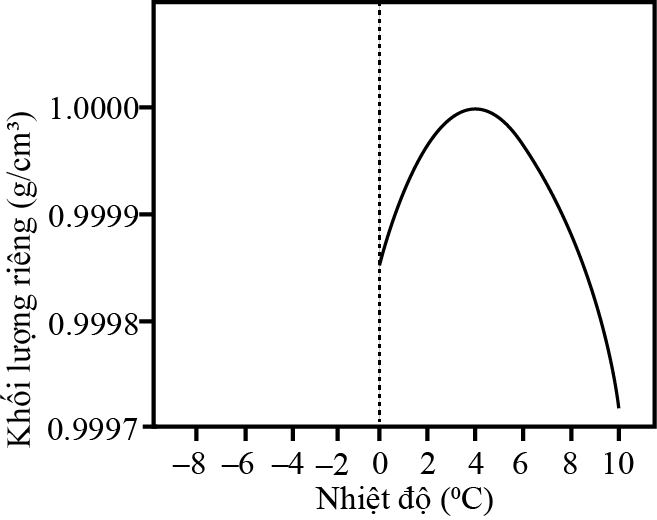
\includegraphics[width=0.5\textwidth]{image/cdle05_image1.png}
\end{center}
\figcaption{1}{Biến thiên về khối lượng riêng của nước ở pha lỏng.}

\begin{center}
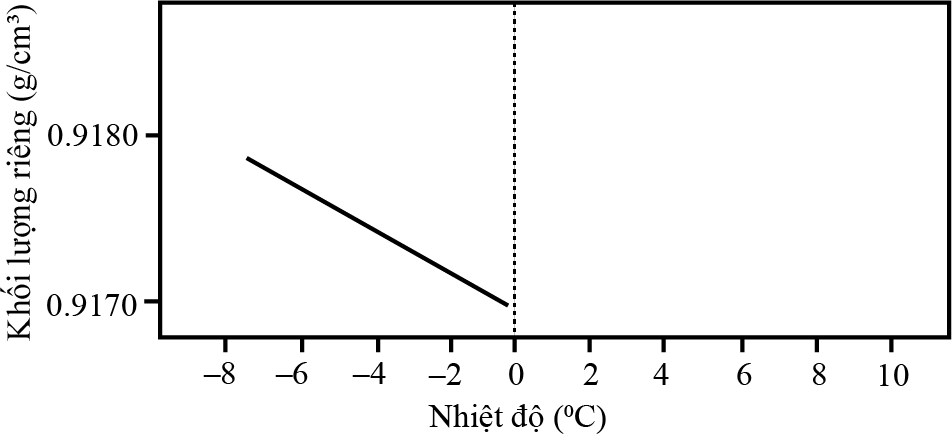
\includegraphics[width=0.5\textwidth]{image/cdle05_image2.png}
\end{center}
\figcaption{2}{Biến thiên về khối lượng riêng của nước ở pha rắn.}

\hfill\textbf{Nguồn: ACT -- American College Testing}
\end{readingpassage}
\vspace{2pt}
\question[Trắc nghiệm]{Theo Hình 2, 1 lít nước ở thể rắn tại 0\,$^{\circ}$C có khối lượng xấp xỉ bao nhiêu?}
\par\vspace{4pt}
\noindent\choiceitem{A}{917 gam.}\hfill\choiceitem{B}{999 gam.}\hfill\choiceitem{C}{1000 gam.}\hfill\choiceitem{D}{1100 gam.}
\question[Trắc nghiệm]{Dựa vào Bảng 1, đơn chất kim loại nào sau đây có khối lượng riêng lớn nhất ở điều kiện 25\,$^{\circ}$C và 1\,atm?}
\par\vspace{4pt}
\noindent\choiceitem{A}{Iron (sắt).}\hfill\choiceitem{B}{Lead (chì).}\hfill\choiceitem{C}{Zinc (kẽm).}\hfill\choiceitem{D}{Arsenic.}
\question[Đúng/Sai]{Cho biết tính Đúng/Sai của các nhận định sau:}

\truefalsehead
\truefalseitem{Theo Hình 2, khối lượng riêng của nước pha rắn giảm dần khi nhiệt độ giảm dần.}
\truefalseitem{Từ Hình 1 và Hình 2, ta có thể kết luận rằng nước pha rắn nổi trên mặt nước pha lỏng.}
\truefalseitem{Trong Bảng 1, mọi chất ở thể rắn đều có khối lượng riêng lớn hơn các chất ở thể lỏng tại điều kiện nhiệt độ 25\,$^{\circ}$C và áp suất 1\,atm.}
\truefalseitem{1\,kg sắt có thể tích lớn hơn 1\,kg chì.}
\truefalseend
\question[Trắc nghiệm]{Theo Hình 1, khi nhiệt độ của nước lỏng giảm từ 10$^{\circ}$C xuống 0$^{\circ}$C, khối lượng riêng:}
\par\vspace{4pt}
\noindent\hangindent=2.2em\hangafter=1\choiceitem{A}{Chỉ tăng dần.}\par\vspace{4pt}
\noindent\hangindent=2.2em\hangafter=1\choiceitem{B}{Chỉ giảm dần.}\par\vspace{4pt}
\noindent\hangindent=2.2em\hangafter=1\choiceitem{C}{Giảm dần rồi tăng dần.}\par\vspace{4pt}
\noindent\hangindent=2.2em\hangafter=1\choiceitem{D}{Tăng dần rồi giảm dần.}\par\vspace{4pt}
\question[Trắc nghiệm]{Một học sinh cho rằng: ``Khi so sánh khối lượng của 1\,cm$^3$ chất rắn bất kỳ với khối lượng của 1\,cm$^3$ chất lỏng bất kỳ, khối lượng của chất rắn sẽ luôn lớn hơn.'' Dữ liệu từ Bảng 1 có ủng hộ giả thuyết này không?}
\par\vspace{4pt}
\noindent\hangindent=2.2em\hangafter=1\choiceitem{A}{Không; chì có khối lượng riêng lớn hơn bất kỳ chất lỏng đã liệt kê.}\par\vspace{4pt}
\noindent\hangindent=2.2em\hangafter=1\choiceitem{B}{Không; thủy ngân có khối lượng riêng lớn hơn bất kỳ chất rắn đã liệt kê.}\par\vspace{4pt}
\noindent\hangindent=2.2em\hangafter=1\choiceitem{C}{Có; chì có khối lượng riêng lớn hơn bất kỳ chất lỏng đã liệt kê.}\par\vspace{4pt}
\noindent\hangindent=2.2em\hangafter=1\choiceitem{D}{Có; thủy ngân có khối lượng riêng lớn hơn bất kỳ chất rắn đã liệt kê.}\par\vspace{4pt}
\question[Ghép đôi]{Ghép đôi mỗi mô tả ở Cột A với chất phù hợp nhất ở Cột B dựa vào Bảng 1.}

\vspace{6pt}
\setstretch{1.3}

\textit{Cột B:}
\vspace{-6pt}
\par\vspace{4pt}
\noindent\hangindent=2.2em\hangafter=1\choiceitem{A}{Ethyl ether}\par\vspace{4pt}
\noindent\hangindent=2.2em\hangafter=1\choiceitem{B}{Glucose}\par\vspace{4pt}
\noindent\hangindent=2.2em\hangafter=1\choiceitem{C}{Lead (chì)}\par\vspace{4pt}
\noindent\hangindent=2.2em\hangafter=1\choiceitem{D}{Methane}\par\vspace{4pt}
\noindent\hangindent=2.2em\hangafter=1\choiceitem{E}{Krypton}\par\vspace{4pt}

\vspace{6pt}

\renewcommand{\arraystretch}{1.6}
{\small\setstretch{1.0}
\begin{longtable}{|>{\raggedright\arraybackslash}m{0.44\textwidth}|>{\centering\arraybackslash}m{0.44\textwidth}|}
\hline
\rowcolor{primaryBlue!12}
\multicolumn{1}{|c|}{\cellcolor{primaryBlue!12}\textbf{Cột A}} & \cellcolor{primaryBlue!12}\textbf{Cột B} \\
\hline
\endfirsthead
\hline
\rowcolor{primaryBlue!12}
\multicolumn{1}{|c|}{\cellcolor{primaryBlue!12}\textbf{Cột A}} & \cellcolor{primaryBlue!12}\textbf{Cột B} \\
\hline
\endhead
1. Kim loại có khối lượng riêng lớn nhất & \dropbox[2.5cm] \\
\hline
2. Chất lỏng nhẹ nhất & \dropbox[2.5cm] \\
\hline
3. Chất khí có khối lượng riêng nhỏ nhất & \dropbox[2.5cm] \\
\hline
4. Chất rắn nhẹ nhất & \dropbox[2.5cm] \\
\hline
\end{longtable}
}
\question[Đúng/Sai]{Cùng một lượng ethyl ether, thủy ngân và nước (khối lượng riêng = 0,9971\,g/cm$^3$) ở nhiệt độ 25$^{\circ}$C đổ vào một phễu chiết. Dung dịch tách thành 3 lớp riêng biệt. Cho biết tính Đúng/Sai của các nhận định sau:}

\truefalsehead
\truefalseitem{Ethyl ether nằm ở lớp trên cùng.}
\truefalseitem{Khi mở khóa ở đáy phễu chiết, thu được nước đầu tiên.}
\truefalseitem{Thủy ngân nằm ở lớp dưới cùng.}
\truefalseitem{Glycerol có thể hòa tan vào lớp nước vì có khối lượng riêng gần với nước.}
\truefalseend
\question[Trắc nghiệm]{Theo Hình 1, với 100\,g nước ở nhiệt độ 4$^{\circ}$C có thể lấp vừa đầy được bình có thể tích là:}
\par\vspace{4pt}
\noindent\choiceitem{A}{1\,cm$^3$.}\hfill\choiceitem{B}{10\,cm$^3$.}\hfill\choiceitem{C}{100\,cm$^3$.}\hfill\choiceitem{D}{1000\,cm$^3$.}
\question[Trắc nghiệm]{Biogas là một loại khí sinh học chứa lên tới 65\% khí methane. Trang trại A trung bình mỗi ngày thu được 12\,m$^3$ biogas. Dựa vào Bảng 1, khối lượng khí methane trung bình thu được mỗi ngày của trang trại A xấp xỉ:}
\par\vspace{4pt}
\noindent\choiceitem{A}{5\,kg.}\hfill\choiceitem{B}{6\,kg.}\hfill\choiceitem{C}{7\,kg.}\hfill\choiceitem{D}{8\,kg.}
\question[Kéo thả]{Kéo thả các từ khóa sau vào chỗ trống:}
\vspace{-4pt}
\dragitems{
\centering
    \dragitem{4} \dragitem{0} \dragitem{100} \dragitem{đơn vị} \\[1pt]
    \dragitem{tiêu chuẩn} \dragitem{giảm} \dragitem{tăng}
}

\setstretch{1.4}
Ở áp suất thường, nước (lỏng) có khối lượng riêng lớn nhất ở (1)\,\dropbox[2cm]$^{\circ}$C. Trị số khối lượng riêng của 1\,cm$^3$ nước ở tại nhiệt độ này được lấy làm (2)\,\dropbox[2.5cm] của khối lượng và gọi là gam.

Khi đun nóng nước lên trên nhiệt độ đó hoặc làm lạnh xuống dưới nhiệt độ đó, khối lượng riêng của nước đều (3)\,\dropbox[2cm].

% ─────────────────────────────────────────────────────────────
% CHỦ ĐỀ 06: KHÍ THẢI NHÀ KÍNH (thuộc B.II.1.1)
% ─────────────────────────────────────────────────────────────
\newpage
\setcounter{qcounter}{0}

\phantomsection\label{b1_cd06}
\begin{topicbox}{\large CHỦ ĐỀ 06: KHÍ THẢI NHÀ KÍNH}
\vspace{8pt}
\textit{Đọc đoạn văn sau và trả lời các câu hỏi.}
\vspace{6pt}
\end{topicbox}
\vspace{5pt}
\begin{readingpassage}[]
\setstretch{1.3}
Khí thải nhà kính, điển hình là CH\textsubscript{4}, làm khí hậu của Trái Đất nóng lên.

Hình 1 biểu diễn nồng độ khí CH\textsubscript{4} trong khí quyển Trái Đất và cường độ bức xạ Mặt Trời lên bề mặt Trái Đất tại các vùng nhiệt đới lục địa Á, Âu từ 250.000 năm trước đến nay. Biểu đồ này cho thấy cả hai tham số trên biến động mạnh mẽ trong khoảng thời gian này. Hình 2 biểu diễn chi tiết hơn về hai số liệu nồng độ khí CH\textsubscript{4} trong khí quyển Trái Đất và cường độ bức xạ Mặt Trời lên bề mặt Trái Đất tại cùng khu vực khảo sát trong vòng 11.000 năm qua. Dữ liệu này đồng nhất với giả thuyết rằng khí thải nhà kính sinh ra từ hoạt động của con người đã đẩy quá trình nóng lên toàn cầu sớm hơn hàng ngàn năm so với từng chu kỳ biến đổi khí hậu trước đây.

\begin{center}
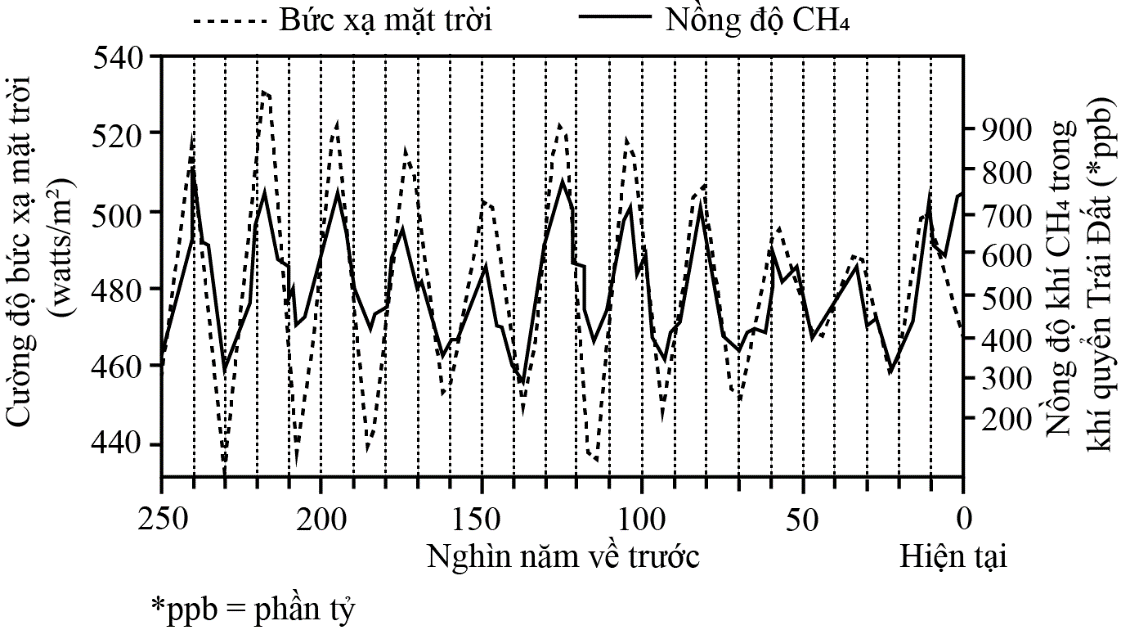
\includegraphics[width=0.75\textwidth]{image/cdle06_image1.png}
\end{center}
\figcaption{1}{Cường độ bức xạ Mặt Trời và nồng độ khí CH\textsubscript{4} từ 250\,000 năm trước đến nay.}

\begin{center}
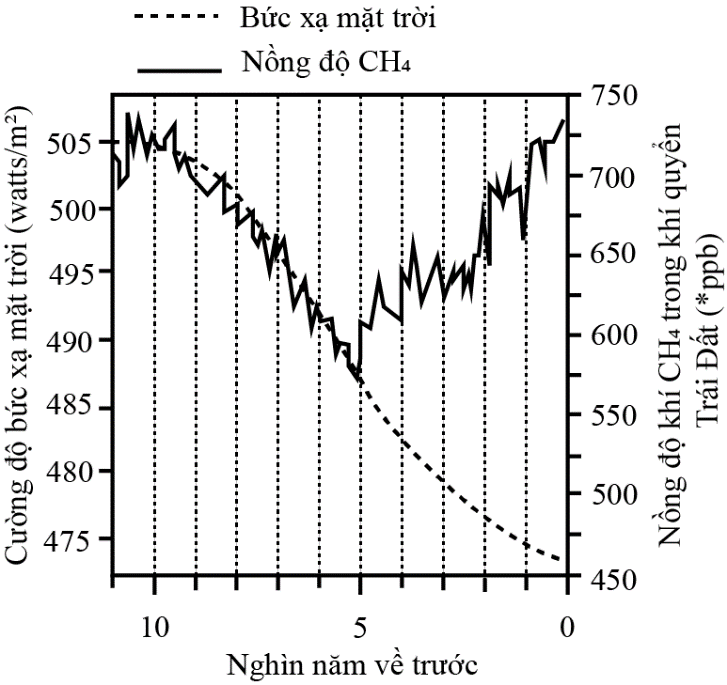
\includegraphics[width=0.55\textwidth]{image/cdle06_image2.png}
\end{center}
\figcaption{2}{Cường độ bức xạ Mặt Trời và nồng độ khí CH\textsubscript{4} từ 11\,000 năm trước đến nay.}

\hfill\textbf{Nguồn: ACT -- American College Testing}
\end{readingpassage}
\vspace{2pt}
\question[Đúng/Sai]{Dựa vào dữ liệu được đưa ra, cho biết tính Đúng/Sai của các nhận định sau:}

\truefalsehead
\truefalseitem{Theo hai đồ thị trên, cường độ bức xạ Mặt Trời trong khoảng 11.000 năm về trước đến nay đang theo xu hướng tăng dần.}
\truefalseitem{Theo Hình 2, nồng độ khí methane tại thời điểm hiện tại đang dần đạt tới nồng độ khí CH\textsubscript{4} cao nhất trong khoảng 11.000 năm về trước.}
\truefalseitem{Khoảng 50.000 năm về trước, nồng độ CH\textsubscript{4} trong khí quyển nằm trong khoảng 550 đến 600\,ppb.}
\truefalseitem{Trong khoảng từ 5.000 năm trước đến nay, nồng độ khí CH\textsubscript{4} biến đổi theo cường độ bức xạ Mặt Trời.}
\truefalseend
\question[Trắc nghiệm]{Theo Hình 2, cường độ bức xạ mặt trời 8.000 năm trước gần nhất với giá trị nào dưới đây?}
\par\vspace{4pt}
\noindent\hangindent=2.2em\hangafter=1\choiceitem{A}{490\,watts/m$^2$.}\par\vspace{4pt}
\noindent\hangindent=2.2em\hangafter=1\choiceitem{B}{495\,watts/m$^2$.}\par\vspace{4pt}
\noindent\hangindent=2.2em\hangafter=1\choiceitem{C}{500\,watts/m$^2$.}\par\vspace{4pt}
\noindent\hangindent=2.2em\hangafter=1\choiceitem{D}{505\,watts/m$^2$.}\par\vspace{4pt}
\question[Trắc nghiệm]{Theo Hình 2, nếu nồng độ khí CH\textsubscript{4} tiếp tục biến đổi theo cường độ bức xạ Mặt Trời, nồng độ khí CH\textsubscript{4} hiện tại sẽ nằm trong khoảng:}
\par\vspace{4pt}
\noindent\hangindent=2.2em\hangafter=1\choiceitem{A}{nhỏ hơn 550\,ppb.}\par\vspace{4pt}
\noindent\hangindent=2.2em\hangafter=1\choiceitem{B}{từ 550\,ppb đến 600\,ppb.}\par\vspace{4pt}
\noindent\hangindent=2.2em\hangafter=1\choiceitem{C}{từ 600\,ppb đến 650\,ppb.}\par\vspace{4pt}
\noindent\hangindent=2.2em\hangafter=1\choiceitem{D}{lớn hơn 650\,ppb.}\par\vspace{4pt}
\question[Trắc nghiệm]{Giả sử khi nồng độ CH\textsubscript{4} trong khí quyển tăng, nhiệt độ trung bình toàn cầu lập tức tăng lên theo và lập tức giảm khi nồng độ CH\textsubscript{4} giảm. Dựa vào Hình 2, đồ thị nào dưới đây biểu diễn chính xác nhất nhiệt độ trung bình toàn cầu trong khoảng 11.000 năm về trước?}
\par\vspace{4pt}
\noindent\choiceitem{A}{Đồ thị A.}\hfill\choiceitem{B}{Đồ thị B.}\hfill\choiceitem{C}{Đồ thị C.}\hfill\choiceitem{D}{Đồ thị D.}
\question[Trắc nghiệm]{Dựa vào Hình 1, trung bình cường độ bức xạ Mặt Trời trong khoảng 250.000 năm khảo sát sẽ có giá trị gần nhất với giá trị nào dưới đây?}
\par\vspace{4pt}
\noindent\hangindent=2.2em\hangafter=1\choiceitem{A}{400\,watts/m$^2$.}\par\vspace{4pt}
\noindent\hangindent=2.2em\hangafter=1\choiceitem{B}{440\,watts/m$^2$.}\par\vspace{4pt}
\noindent\hangindent=2.2em\hangafter=1\choiceitem{C}{480\,watts/m$^2$.}\par\vspace{4pt}
\noindent\hangindent=2.2em\hangafter=1\choiceitem{D}{520\,watts/m$^2$.}\par\vspace{4pt}
\question[Trắc nghiệm]{Một chu kì bức xạ Mặt Trời là khoảng thời gian giữa hai điểm cực đại cường độ bức xạ mặt trời liên tiếp. Theo Hình 1, trung bình thời gian của một chu kì bức xạ trong khoảng 250.000 năm qua nằm trong khoảng:}
\par\vspace{4pt}
\noindent\hangindent=2.2em\hangafter=1\choiceitem{A}{nhỏ hơn 15.000 năm.}\par\vspace{4pt}
\noindent\hangindent=2.2em\hangafter=1\choiceitem{B}{từ 15.000 năm đến 35.000 năm.}\par\vspace{4pt}
\noindent\hangindent=2.2em\hangafter=1\choiceitem{C}{từ 35.000 năm đến 55.000 năm.}\par\vspace{4pt}
\noindent\hangindent=2.2em\hangafter=1\choiceitem{D}{lớn hơn 55.000 năm.}\par\vspace{4pt}
\question[Trắc nghiệm]{Mệnh đề nào dưới đây chỉ ra chính xác nhất hiệu ứng chính của khí methane lên khí hậu Trái Đất?}
\par\vspace{4pt}
\noindent\hangindent=2.2em\hangafter=1\choiceitem{A}{CH\textsubscript{4} phản chiếu lại ánh sáng khả kiến ra không gian, hạ nhiệt độ Trái Đất.}\par\vspace{4pt}
\noindent\hangindent=2.2em\hangafter=1\choiceitem{B}{CH\textsubscript{4} phản chiếu lại bức xạ cực tím ra không gian, làm tăng nhiệt độ Trái Đất.}\par\vspace{4pt}
\noindent\hangindent=2.2em\hangafter=1\choiceitem{C}{CH\textsubscript{4} hấp thụ nhiệt đi từ không gian vào tầng khí quyển, hạ nhiệt độ Trái Đất.}\par\vspace{4pt}
\noindent\hangindent=2.2em\hangafter=1\choiceitem{D}{CH\textsubscript{4} hấp thụ nhiệt tỏa ra từ bề mặt Trái Đất.}\par\vspace{4pt}
\question[Kéo thả]{Kéo thả các từ khóa sau vào chỗ trống:}
\vspace{-4pt}
\dragitems{
\centering
    \dragitem{CO\textsubscript{2}} \dragitem{H\textsubscript{2}O} \dragitem{CH\textsubscript{4}} \dragitem{cao} \\[1pt]
    \dragitem{thấp} \dragitem{nhà kính} \dragitem{lồng kính} \dragitem{sóng ngắn} \\[1pt]
    \dragitem{sóng dài}
}

\setstretch{1.4}
Ngoài methane, các tác nhân nổi bật góp phần gây nên hiệu ứng nhà kính là carbon dioxide (công thức hoá học là (1)\,\dropbox[2cm]) và hơi nước (H\textsubscript{2}O). Khi các tia bức xạ sóng ngắn (ứng với mức năng lượng (2)\,\dropbox[2cm]) của Mặt Trời xuyên qua bầu khí quyển đến mặt đất và được phản xạ lại từ bề mặt Trái Đất qua các tia bức xạ sóng dài (ứng với năng lượng (3)\,\dropbox[2cm]), các phân tử khí nhà kính sẽ hấp thụ một phần bức xạ sóng dài này từ đó làm bầu khí quyển ấm lên, biến Trái Đất thành một (4)\,\dropbox[2.5cm].
\question[Điền khuyết]{Dựa vào Hình 1 và Hình 2, điền từ/cụm từ thích hợp (không quá 3 tiếng) vào chỗ trống:}

\vspace{5pt}
\setstretch{1.4}
\begin{itemize}[leftmargin=*, itemsep=5pt, topsep=0pt, partopsep=0pt, parsep=0pt, label=\textcolor{primaryBlue}{\textbullet}]
\item Theo Hình 1, nồng độ CH\textsubscript{4} đạt giá trị cao nhất vào khoảng (1)\,\dropbox[2.5cm] nghìn năm trước.
\item Theo Hình 2, trong khoảng 5.000 năm gần đây, nồng độ CH\textsubscript{4} có xu hướng (2)\,\dropbox[2cm] trong khi cường độ bức xạ Mặt Trời có xu hướng (3)\,\dropbox[2cm], cho thấy sự tách rời giữa hai đại lượng này.
\end{itemize}
\question[Ghép đôi]{Ghép đôi mỗi khoảng thời gian ở Cột A với xu hướng đúng nhất ở Cột B dựa vào Hình 1 và Hình 2.}

\vspace{6pt}
\setstretch{1.3}

\textit{Cột B:}
\vspace{-6pt}
\par\vspace{4pt}
\noindent\hangindent=2.2em\hangafter=1\choiceitem{A}{CH\textsubscript{4} tăng cùng chiều với bức xạ Mặt Trời}\par\vspace{4pt}
\noindent\hangindent=2.2em\hangafter=1\choiceitem{B}{CH\textsubscript{4} giảm cùng chiều với bức xạ Mặt Trời}\par\vspace{4pt}
\noindent\hangindent=2.2em\hangafter=1\choiceitem{C}{CH\textsubscript{4} tăng trong khi bức xạ Mặt Trời giảm}\par\vspace{4pt}
\noindent\hangindent=2.2em\hangafter=1\choiceitem{D}{CH\textsubscript{4} giảm trong khi bức xạ Mặt Trời tăng}\par\vspace{4pt}

\vspace{6pt}

\renewcommand{\arraystretch}{1.6}
{\small\setstretch{1.0}
\begin{longtable}{|>{\raggedright\arraybackslash}m{0.44\textwidth}|>{\centering\arraybackslash}m{0.44\textwidth}|}
\hline
\rowcolor{primaryBlue!12}
\multicolumn{1}{|c|}{\cellcolor{primaryBlue!12}\textbf{Cột A}} & \cellcolor{primaryBlue!12}\textbf{Cột B} \\
\hline
\endfirsthead
\hline
\rowcolor{primaryBlue!12}
\multicolumn{1}{|c|}{\cellcolor{primaryBlue!12}\textbf{Cột A}} & \cellcolor{primaryBlue!12}\textbf{Cột B} \\
\hline
\endhead
1. 250.000 -- 200.000 năm trước & \dropbox[2.5cm] \\
\hline
2. 125.000 -- 100.000 năm trước & \dropbox[2.5cm] \\
\hline
3. 11.000 -- 5.000 năm trước & \dropbox[2.5cm] \\
\hline
4. 5.000 năm trước -- hiện tại & \dropbox[2.5cm] \\
\hline
\end{longtable}
}

% ─────────────────────────────────────────────────────────────
% CHỦ ĐỀ 07: NHỰA (thuộc B.II.1.1)
% ─────────────────────────────────────────────────────────────
\newpage
\setcounter{qcounter}{0}

\phantomsection\label{b1_cd07}
\begin{topicbox}{\large CHỦ ĐỀ 07: NHỰA}
\vspace{8pt}
\textit{Đọc đoạn văn sau và trả lời các câu hỏi.}
\vspace{6pt}
\end{topicbox}
\vspace{5pt}
\begin{readingpassage}[]
\setstretch{1.3}
Một số học sinh tiến hành thí nghiệm để đo khối lượng riêng một số loại nhựa phổ biến.

\textbf{Thí nghiệm 1:} Học sinh A đặt một ống đong khô dung tích 100\,mL lên cân điện tử và trừ bì (hiệu chỉnh, đưa số trên cân về 0,000\,g). Thêm một khối lượng nước cố định, sau đó thêm ethanol đến vạch 50,0\,mL. Tiếp theo tính khối lượng riêng của dung dịch trong ống. Thí nghiệm được lặp lại với lượng ethanol và nước khác nhau. Kết quả được tổng hợp trong Bảng 1.

\tablecaption{1}{Khối lượng riêng của dung dịch 1 -- 5.}
\renewcommand{\arraystretch}{1.3}
{\small
\setstretch{1.0}%
\begin{center}
\begin{tabular}{|c|c|c|c|c|}
\hline
\rowcolor{primaryBlue!12}
\textbf{DD} & \textbf{KL nước (g)} & \textbf{KL ethanol (g)} & \textbf{Tổng KL (g)} & \textbf{KLR (g/mL)} \\
\hline
1 & 0 & 39,67 & 39,67 & 0,793 \\
\hline
2 & 10,24 & 32,43 & 42,67 & 0,853 \\
\hline
3 & 19,79 & 25,23 & 45,02 & 0,900 \\
\hline
4 & 35,42 & 12,47 & 47,89 & 0,958 \\
\hline
5 & 49,96 & 0 & 49,96 & 0,999 \\
\hline
\end{tabular}
\end{center}
}

\vspace{6pt}
\textbf{Thí nghiệm 2:} Một lượng potassium iodide (KI) đã biết được đem hòa tan vào một lượng nước đã biết. Sau khi cân và trừ bì một ống đong khô 100\,mL, dung dịch đã pha được cho vào ống đến vạch 50,0\,mL. Dựa vào cân nặng, khối lượng riêng của dung dịch được tính ra và ghi vào bảng. Lặp lại thí nghiệm với lượng KI và nước khác nhau. Kết quả được tổng hợp trong Bảng 2.

\tablecaption{2}{Khối lượng riêng của dung dịch 6 -- 10.}
\renewcommand{\arraystretch}{1.3}
{\small
\setstretch{1.0}%
\begin{center}
\begin{tabular}{|c|c|c|c|c|}
\hline
\rowcolor{primaryBlue!12}
\textbf{DD} & \textbf{KL nước (g)} & \textbf{KL KI (g)} & \textbf{Tổng KL (g)} & \textbf{KLR (g/mL)} \\
\hline
6 & 97,66 & 7,36 & 52,51 & 1,05 \\
\hline
7 & 95,41 & 15,52 & 55,70 & 1,11 \\
\hline
8 & 94,38 & 20,68 & 57,53 & 1,15 \\
\hline
9 & 92,18 & 29,08 & 60,63 & 1,21 \\
\hline
10 & 87,77 & 41,31 & 64,64 & 1,29 \\
\hline
\end{tabular}
\end{center}
}

\vspace{6pt}
\textbf{Thí nghiệm 3:} Một số hạt nhựa cứng được đặt vào đáy ống mẫu của 10 loại dung dịch đã pha trong thí nghiệm 1 và 2. Nếu hạt nằm nguyên dưới đáy, ghi vào bảng là ``C'', còn nếu hạt di chuyển lên bề mặt dung dịch, ghi vào bảng là ``N''. Thí nghiệm lặp lại với nhiều loại nhựa khác nhau. Kết quả được tổng hợp ở Bảng 3.

\tablecaption{3}{Kết quả khi thả các viên nhựa vào từng dung dịch.}
\renewcommand{\arraystretch}{1.3}
{\footnotesize
\setstretch{1.0}%
\begin{center}
\begin{tabular}{|l|c|c|c|c|c|c|c|c|c|c|}
\hline
\rowcolor{primaryBlue!12}
\textbf{Nhựa} & \textbf{1} & \textbf{2} & \textbf{3} & \textbf{4} & \textbf{5} & \textbf{6} & \textbf{7} & \textbf{8} & \textbf{9} & \textbf{10} \\
\hline
Polybutylene & N & N & N & N & N & N & N & N & N & N \\
\hline
VLDPE & C & N & N & N & N & N & N & N & N & N \\
\hline
LDPE & C & C & C & N & N & N & N & N & N & N \\
\hline
HDPE & C & C & C & C & N & N & N & N & N & N \\
\hline
PA-11 & C & C & C & C & C & N & N & N & N & N \\
\hline
PA-6 & C & C & C & C & C & C & C & N & N & N \\
\hline
Polycarbonate & C & C & C & C & C & C & C & C & N & N \\
\hline
PVC & C & C & C & C & C & C & C & C & C & C \\
\hline
\end{tabular}
\end{center}
}

\hfill\textbf{Nguồn: ACT -- American College Testing}
\end{readingpassage}
\vspace{2pt}
\question[Trắc nghiệm]{Để pha được 50,0\,mL dung dịch KI có khối lượng riêng 1,21\,g/mL, cần hòa tan bao nhiêu gam KI vào 92,18\,g nước cất? (Theo Bảng 2)}
\par\vspace{4pt}
\noindent\choiceitem{A}{7,36\,g.}\hfill\choiceitem{B}{15,52\,g.}\hfill\choiceitem{C}{29,08\,g.}\hfill\choiceitem{D}{41,31\,g.}
\question[Đúng/Sai]{Dựa vào dữ liệu trên, cho biết tính Đúng/Sai của các nhận định sau:}

\truefalsehead
\truefalseitem{Nhựa PA-6 là nhựa nhẹ nhất trong số các nhựa đã khảo sát.}
\truefalseitem{Nếu thả viên nhựa PVC và viên nhựa PA-11 vào dung dịch số 7, cả hai viên nhựa sẽ nằm trên bề mặt dung dịch.}
\truefalseitem{Nhựa HDPE nặng hơn nhựa VLDPE.}
\truefalseitem{Nhựa polycarbonate là nhựa nặng nhất trong số các nhựa đã khảo sát.}
\truefalseitem{Ethanol nhẹ hơn nước ở điều kiện thường.}
\truefalseend
\question[Trắc nghiệm]{Trong thí nghiệm 1, khối lượng riêng của ethanol nằm trong khoảng giá trị nào?}
\par\vspace{4pt}
\noindent\hangindent=2.2em\hangafter=1\choiceitem{A}{Nhỏ hơn 0,793\,g/mL.}\par\vspace{4pt}
\noindent\hangindent=2.2em\hangafter=1\choiceitem{B}{0,793\,g/mL.}\par\vspace{4pt}
\noindent\hangindent=2.2em\hangafter=1\choiceitem{C}{0,999\,g/mL.}\par\vspace{4pt}
\noindent\hangindent=2.2em\hangafter=1\choiceitem{D}{Lớn hơn 0,999\,g/mL.}\par\vspace{4pt}
\question[Trắc nghiệm]{Dựa vào 3 thí nghiệm, khối lượng riêng của nhựa PA-11 sẽ nằm trong khoảng:}
\par\vspace{4pt}
\noindent\hangindent=2.2em\hangafter=1\choiceitem{A}{nhỏ hơn 0,793\,g/mL.}\par\vspace{4pt}
\noindent\hangindent=2.2em\hangafter=1\choiceitem{B}{từ 0,853\,g/mL đến 0,958\,g/mL.}\par\vspace{4pt}
\noindent\hangindent=2.2em\hangafter=1\choiceitem{C}{từ 0,999\,g/mL đến 1,05\,g/mL.}\par\vspace{4pt}
\noindent\hangindent=2.2em\hangafter=1\choiceitem{D}{lớn hơn 1,11\,g/mL.}\par\vspace{4pt}
\question[Trắc nghiệm]{Giả sử có dung dịch KI thứ sáu được đo trong thí nghiệm 2 và khối lượng của dung dịch trong ống đong là 67,54\,g. Khối lượng riêng của dung dịch này gần nhất với giá trị:}
\par\vspace{4pt}
\noindent\choiceitem{A}{1,25\,g/mL.}\hfill\choiceitem{B}{1,30\,g/mL.}\hfill\choiceitem{C}{1,35\,g/mL.}\hfill\choiceitem{D}{1,40\,g/mL.}
\question[Trắc nghiệm]{Một hạt nhựa khác được thử trong thí nghiệm 3. Bộ kết quả nào dưới đây KHÔNG phải của hạt nhựa?}
\par\vspace{4pt}
\noindent\hangindent=2.2em\hangafter=1\choiceitem{A}{1(N) -- 2(N) -- 3(N) -- 4(N).}\par\vspace{4pt}
\noindent\hangindent=2.2em\hangafter=1\choiceitem{B}{1(N) -- 2(N) -- 3(C) -- 4(C).}\par\vspace{4pt}
\noindent\hangindent=2.2em\hangafter=1\choiceitem{C}{1(C) -- 2(C) -- 3(N) -- 4(N).}\par\vspace{4pt}
\noindent\hangindent=2.2em\hangafter=1\choiceitem{D}{1(C) -- 2(C) -- 3(C) -- 4(C).}\par\vspace{4pt}
\question[Trắc nghiệm]{Trong thí nghiệm 1 và 2, bước trừ bì giúp xác định:}
\par\vspace{4pt}
\noindent\hangindent=2.2em\hangafter=1\choiceitem{A}{khối lượng của dung dịch trong ống đong.}\par\vspace{4pt}
\noindent\hangindent=2.2em\hangafter=1\choiceitem{B}{khối lượng riêng của ống đong.}\par\vspace{4pt}
\noindent\hangindent=2.2em\hangafter=1\choiceitem{C}{tín hiệu khi dung dịch cho vào đủ 50,0\,mL.}\par\vspace{4pt}
\noindent\hangindent=2.2em\hangafter=1\choiceitem{D}{tín hiệu khi tất cả KI đã tan trong nước.}\par\vspace{4pt}
\question[Trắc nghiệm]{Một học sinh cho rằng nhựa polycarbonate nặng hơn nhựa PA-6. Kết quả của ba thí nghiệm có ủng hộ nhận định này không?}
\par\vspace{4pt}
\noindent\hangindent=2.2em\hangafter=1\choiceitem{A}{Không, vì trong dung dịch 8, hạt polycarbonate nằm dưới đáy ống còn hạt PA-6 nổi.}\par\vspace{4pt}
\noindent\hangindent=2.2em\hangafter=1\choiceitem{B}{Có, vì trong dung dịch 8, hạt polycarbonate nằm dưới đáy ống còn hạt PA-6 nổi.}\par\vspace{4pt}
\noindent\hangindent=2.2em\hangafter=1\choiceitem{C}{Không, vì trong dung dịch 8, hạt polycarbonate nổi còn hạt PA-6 nằm dưới đáy ống.}\par\vspace{4pt}
\noindent\hangindent=2.2em\hangafter=1\choiceitem{D}{Có, vì trong dung dịch 8, hạt polycarbonate nổi còn hạt PA-6 nằm dưới đáy ống.}\par\vspace{4pt}
\question[Kéo thả]{Kéo thả các từ/cụm từ sau vào chỗ trống:}
\vspace{-4pt}
\dragitems{
\centering
    \dragitem{PVC} \dragitem{polybutylene} \dragitem{VLDPE} \dragitem{0,793} \\[1pt]
    \dragitem{0,999} \dragitem{1,29} \dragitem{chìm} \dragitem{nổi}
}

\setstretch{1.4}
Trong các loại nhựa đã khảo sát, (1)\,\dropbox[2.5cm] là loại nhựa nặng nhất vì chìm trong tất cả 10 dung dịch. Ngược lại, (2)\,\dropbox[2.5cm] là loại nhựa nhẹ nhất vì nổi trong tất cả 10 dung dịch, cho thấy khối lượng riêng của nó nhỏ hơn (3)\,\dropbox[2cm]\,g/mL.
\question[Ghép đôi]{Ghép đôi mỗi loại nhựa ở Cột A với khoảng khối lượng riêng phù hợp nhất ở Cột B, dựa vào kết quả Bảng 3.}

\vspace{6pt}
\setstretch{1.3}

\textit{Cột B:}
\vspace{-6pt}
\par\vspace{4pt}
\noindent\hangindent=2.2em\hangafter=1\choiceitem{A}{0,958 -- 0,999\,g/mL}\par\vspace{4pt}
\noindent\hangindent=2.2em\hangafter=1\choiceitem{B}{0,900 -- 0,958\,g/mL}\par\vspace{4pt}
\noindent\hangindent=2.2em\hangafter=1\choiceitem{C}{1,11 -- 1,15\,g/mL}\par\vspace{4pt}
\noindent\hangindent=2.2em\hangafter=1\choiceitem{D}{1,15 -- 1,21\,g/mL}\par\vspace{4pt}

\vspace{6pt}

\renewcommand{\arraystretch}{1.6}
{\small\setstretch{1.0}
\begin{longtable}{|>{\raggedright\arraybackslash}m{0.44\textwidth}|>{\centering\arraybackslash}m{0.44\textwidth}|}
\hline
\rowcolor{primaryBlue!12}
\multicolumn{1}{|c|}{\cellcolor{primaryBlue!12}\textbf{Cột A}} & \cellcolor{primaryBlue!12}\textbf{Cột B} \\
\hline
\endfirsthead
\hline
\rowcolor{primaryBlue!12}
\multicolumn{1}{|c|}{\cellcolor{primaryBlue!12}\textbf{Cột A}} & \cellcolor{primaryBlue!12}\textbf{Cột B} \\
\hline
\endhead
1. LDPE & \dropbox[2.5cm] \\
\hline
2. PA-6 & \dropbox[2.5cm] \\
\hline
3. Polycarbonate & \dropbox[2.5cm] \\
\hline
4. HDPE & \dropbox[2.5cm] \\
\hline
\end{longtable}
}

% ─────────────────────────────────────────────────────────────
% CHỦ ĐỀ 08: THỬ NGHIỆM HOẠT TÍNH THUỐC KHÁNG SINH (thuộc B.II.1.1)
% ─────────────────────────────────────────────────────────────
\newpage
\setcounter{qcounter}{0}

\phantomsection\label{b1_cd08}
\begin{topicbox}{\large CHỦ ĐỀ 08: THỬ NGHIỆM HOẠT TÍNH THUỐC KHÁNG SINH}
\vspace{8pt}
\textit{Đọc đoạn văn sau và trả lời các câu hỏi.}
\vspace{6pt}
\end{topicbox}
\vspace{5pt}
\begin{readingpassage}[]
\setstretch{1.3}
Một nhà khoa học đã thử nghiệm khả năng tiêu diệt một chủng vi khuẩn kháng penicillin của 5 loại thuốc mới được chế tạo.

\textbf{Thí nghiệm 1:} Số lượng vi khuẩn kháng penicillin bằng nhau được cho vào các bình chứa 10,0\,mL môi trường dinh dưỡng. Các bình được ủ trong 1 giờ ở 37$^{\circ}$C với các nồng độ khác nhau của 5 loại thuốc. Lô đối chứng nuôi vi khuẩn trong môi trường không có bất kỳ loại thuốc nào. Sau khi ủ 1 giờ, vi khuẩn được rửa để loại bỏ vết thuốc còn sót lại và được cấy lên đĩa thạch dinh dưỡng trong 7 ngày. Trong thời gian này, vi khuẩn sinh sản, tạo thành các khuẩn lạc, sau đó được đếm vào cuối ngày thứ bảy. Lô đối chứng sau 7 ngày đếm được 50 khuẩn lạc trên đĩa nuôi cấy. Cách bố trí và kết quả của Thí nghiệm 1 thể hiện ở Bảng 1.

\tablecaption{1}{Hoạt tính của thuốc tính theo nồng độ (số khuẩn lạc đếm được sau 7 ngày).}
\renewcommand{\arraystretch}{1.3}
{\small
\setstretch{1.0}%
\begin{center}
\begin{tabular}{|l|c|c|c|c|}
\hline
\rowcolor{primaryBlue!12}
\textbf{Thuốc} & \textbf{5\,mM} & \textbf{10\,mM} & \textbf{15\,mM} & \textbf{25\,mM} \\
\hline
R & 41 & 26 & 9 & 0 \\
\hline
S & 42 & 29 & 12 & 2 \\
\hline
T & 45 & 35 & 20 & 5 \\
\hline
U & 47 & 38 & 21 & 6 \\
\hline
V & 50 & 40 & 22 & 7 \\
\hline
\end{tabular}
\end{center}
}

\vspace{6pt}
\textbf{Thí nghiệm 2:} Vi khuẩn được xử lí giống Thí nghiệm 1 nhưng có hai thay đổi: thứ nhất, tất cả các loại thuốc được thử nghiệm ở cùng một nồng độ; thứ hai, áp dụng nhiều khoảng thời gian ủ với từng loại thuốc. Bảng 2 cho thấy số lượng khuẩn lạc được đếm.

\tablecaption{2}{Hoạt tính của thuốc tính theo thời gian ủ (số khuẩn lạc đếm được sau 7 ngày).}
\renewcommand{\arraystretch}{1.3}
{\small
\setstretch{1.0}%
\begin{center}
\begin{tabular}{|l|c|c|c|c|}
\hline
\rowcolor{primaryBlue!12}
\textbf{Thuốc} & \textbf{1 giờ} & \textbf{6 giờ} & \textbf{12 giờ} & \textbf{24 giờ} \\
\hline
R & 41 & 8 & 2 & 0 \\
\hline
S & 42 & 12 & 4 & 1 \\
\hline
T & 45 & 15 & 6 & 2 \\
\hline
U & 47 & 18 & 7 & 3 \\
\hline
V & 50 & 22 & 9 & 5 \\
\hline
\end{tabular}
\end{center}
}

\hfill\textbf{Nguồn: ACT -- American College Testing}
\end{readingpassage}
\vspace{2pt}
\question[Trắc nghiệm]{Dựa vào Bảng 1, loại thuốc nào thể hiện hoạt tính kháng khuẩn kém nhất ở nồng độ 25\,mM?}
\par\vspace{4pt}
\noindent\choiceitem{A}{Thuốc R.}\hfill\choiceitem{B}{Thuốc S.}\hfill\choiceitem{C}{Thuốc U.}\hfill\choiceitem{D}{Thuốc V.}
\question[Kéo thả]{Kéo các cụm từ thích hợp vào chỗ trống để tóm tắt nguyên lí của bài đọc:}
\vspace{-4pt}
\dragitems{
\centering
    \dragitem{nồng độ} \dragitem{tương quan nghịch} \dragitem{tương quan thuận} \dragitem{thời gian ủ} \\[1pt]
    \dragitem{thuốc R} \dragitem{thuốc V} \dragitem{đối chứng}
}

\setstretch{1.4}
Thí nghiệm 1 cho thấy hoạt tính kháng khuẩn của 5 loại thuốc mới phụ thuộc vào mức (1)\,\dropbox[2.5cm], còn Thí nghiệm 2 cho thấy nó còn phụ thuộc vào mức (2)\,\dropbox[2.5cm]. Số lượng khuẩn lạc sống sót trên đĩa thạch có mối quan hệ (3)\,\dropbox[3cm] với hiệu quả diệt khuẩn của thuốc. Trong số các mẫu thử nghiệm, (4)\,\dropbox[2.5cm] thể hiện hoạt tính mạnh nhất. Để đảm bảo thí nghiệm có giá trị định lượng, sự hiện diện của lô (5)\,\dropbox[2.5cm] là bắt buộc nhằm cung cấp con số nền để tính toán hiệu suất.
\question[Điền khuyết]{Một bệnh viện dự định sử dụng thuốc S để xử lí bề mặt thiết bị nhiễm khuẩn. Nếu sử dụng nồng độ 15\,mM và ủ trong 1 giờ giống điều kiện Thí nghiệm 1, hiệu suất tiêu diệt vi khuẩn của thuốc S đạt bao nhiêu phần trăm?\\[3pt]
\textit{(Làm tròn đến số nguyên gần nhất. Chỉ điền số, không điền kí hiệu \%.)}}

\vspace{5pt}
\setstretch{1.4}
Kết quả: \dropbox[3cm]\,\%

\question[Đúng/Sai]{Một nhóm sinh viên đưa ra các nhận định sau về thiết kế và kết quả của hai thí nghiệm. Các nhận định này đúng hay sai:}

\truefalsehead
\truefalseitem{Lô đối chứng trong Thí nghiệm 1 nhằm xác định số lượng vi khuẩn phát triển tối đa khi không chịu bất kỳ tác động nào của thuốc kháng sinh.}
\truefalseitem{Biến số phụ thuộc (kết quả đo lường) trong cả hai thí nghiệm là hoạt tính của thuốc tính theo phần trăm.}
\truefalseitem{Ở thời gian ủ 24 giờ (Thí nghiệm 2), tất cả 5 loại thuốc đều tiêu diệt hoàn toàn vi khuẩn kháng penicillin.}
\truefalseitem{Số lượng khuẩn lạc phát triển trên đĩa thạch tương quan thuận với hiệu quả kháng khuẩn của loại thuốc được thử nghiệm.}
\truefalseend
\question[Ghép đôi]{Dựa vào dữ liệu từ Bảng 1, ghép tên loại thuốc (Cột A) với đặc điểm hoạt tính tương ứng (Cột B).}

\vspace{6pt}
\setstretch{1.3}

\textit{Cột B:}
\vspace{-6pt}
\par\vspace{4pt}
\noindent\hangindent=2.2em\hangafter=1\choiceitem{A}{Là loại thuốc yếu nhất, có số khuẩn lạc sống sót cao nhất ở mọi nồng độ thử nghiệm.}\par\vspace{4pt}
\noindent\hangindent=2.2em\hangafter=1\choiceitem{B}{Ở nồng độ 25\,mM, thuốc này có hiệu suất tiêu diệt đúng 90\% lượng vi khuẩn so với lô đối chứng.}\par\vspace{4pt}
\noindent\hangindent=2.2em\hangafter=1\choiceitem{C}{Diệt khuẩn tuyệt đối ở nồng độ 25\,mM, không còn vi khuẩn sống sót.}\par\vspace{4pt}
\noindent\hangindent=2.2em\hangafter=1\choiceitem{D}{Ở nồng độ 25\,mM, số vi khuẩn sống sót của thuốc này chỉ bằng 1/3 so với thuốc U.}\par\vspace{4pt}
\noindent\hangindent=2.2em\hangafter=1\choiceitem{E}{Ở nồng độ 10\,mM, thuốc này tiêu diệt đúng một nửa số vi khuẩn so với lô đối chứng.}\par\vspace{4pt}

\vspace{6pt}

\renewcommand{\arraystretch}{1.6}
{\small\setstretch{1.0}
\begin{longtable}{|>{\raggedright\arraybackslash}m{0.44\textwidth}|>{\centering\arraybackslash}m{0.44\textwidth}|}
\hline
\rowcolor{primaryBlue!12}
\multicolumn{1}{|c|}{\cellcolor{primaryBlue!12}\textbf{Cột A}} & \cellcolor{primaryBlue!12}\textbf{Cột B} \\
\hline
\endfirsthead
\hline
\rowcolor{primaryBlue!12}
\multicolumn{1}{|c|}{\cellcolor{primaryBlue!12}\textbf{Cột A}} & \cellcolor{primaryBlue!12}\textbf{Cột B} \\
\hline
\endhead
1. Thuốc R & \dropbox[2.5cm] \\
\hline
2. Thuốc S & \dropbox[2.5cm] \\
\hline
3. Thuốc T & \dropbox[2.5cm] \\
\hline
4. Thuốc V & \dropbox[2.5cm] \\
\hline
\end{longtable}
}
\question[Điền khuyết]{Tính toán và đánh giá tốc độ tiêu diệt vi khuẩn của thuốc U theo dữ liệu Thí nghiệm 2.\\[3pt]
\textit{(Điền số nguyên vào các ô trống.)}}

\vspace{5pt}
\setstretch{1.4}
\begin{itemize}[leftmargin=*, itemsep=5pt, topsep=0pt, partopsep=0pt, parsep=0pt, label=\textcolor{primaryBlue}{\textbullet}]
\item Từ giờ thứ 1 đến giờ thứ 6, số lượng khuẩn lạc khi xử lí bằng thuốc U đã giảm đi (1)\,\dropbox[2.5cm] khuẩn lạc.
\item Nếu chỉ xét riêng khoảng thời gian từ giờ thứ 12 đến giờ thứ 24, thuốc U đã tiêu diệt thêm được xấp xỉ (2)\,\dropbox[2.5cm]\,\% số lượng vi khuẩn còn sống sót tính tại thời điểm mốc 12 giờ.
\end{itemize}

\question[Trắc nghiệm]{Văn bản cho biết ở Thí nghiệm 2, ``tất cả các loại thuốc được thử nghiệm ở cùng một nồng độ'' nhưng không nêu rõ giá trị. Bằng cách đối chiếu dữ liệu giữa Bảng 1 và Bảng 2, nồng độ cố định đã sử dụng trong Thí nghiệm 2 là bao nhiêu?}
\par\vspace{4pt}
\noindent\choiceitem{A}{5\,mM.}\hfill\choiceitem{B}{10\,mM.}\hfill\choiceitem{C}{15\,mM.}\hfill\choiceitem{D}{25\,mM.}
\question[Đúng/Sai]{Các nhà khoa học đang xem xét đưa các loại thuốc này vào thử nghiệm lâm sàng trên cơ thể người. Đánh giá tính hợp lí của các phương án đánh đổi và ngoại suy sau đây:}

\truefalsehead
\truefalseitem{Nếu thuốc R ở nồng độ trên 20\,mM gây độc cho gan người, có thể khắc phục bằng cách dùng thuốc R ở mức nồng độ thấp như trong Thí nghiệm 2 nhưng kéo dài thời gian ủ lên 24 giờ để vẫn đạt hiệu quả diệt khuẩn 100\%.}
\truefalseitem{Nếu mục tiêu y khoa là giữ vi khuẩn sống sót ở mức không quá 5 khuẩn lạc nhưng không được tiêu diệt hoàn toàn, thuốc V ở thời gian ủ 24 giờ là lựa chọn đáp ứng được yêu cầu.}
\truefalseitem{Dựa vào xu hướng của Bảng 2, có thể kết luận chắc chắn rằng mọi loại thuốc đều sẽ tiêu diệt hoàn toàn vi khuẩn (0 khuẩn lạc) nếu thời gian ủ được kéo dài đến 48 giờ.}
\truefalseitem{Để đạt hiệu quả tiêu diệt để lại không quá 7 khuẩn lạc, phương án duy nhất là sử dụng thuốc ở nồng độ 25\,mM.}
\truefalseend
\question[Trắc nghiệm]{Giả sử chi phí sản xuất 1\,mM thuốc R là 10\,USD, trong khi chi phí cho 1\,mM thuốc S chỉ là 2\,USD. Một liệu trình điều trị (ủ 1 giờ như Thí nghiệm 1) yêu cầu số vi khuẩn sống sót không vượt quá 10 khuẩn lạc. Phương án nào sau đây có tổng chi phí thấp nhất mà vẫn đảm bảo hiệu quả?}
\par\vspace{4pt}
\noindent\hangindent=2.2em\hangafter=1\choiceitem{A}{Dùng thuốc R ở nồng độ 15\,mM.}\par\vspace{4pt}
\noindent\hangindent=2.2em\hangafter=1\choiceitem{B}{Dùng thuốc S ở nồng độ 15\,mM.}\par\vspace{4pt}
\noindent\hangindent=2.2em\hangafter=1\choiceitem{C}{Dùng thuốc S ở nồng độ 25\,mM.}\par\vspace{4pt}
\noindent\hangindent=2.2em\hangafter=1\choiceitem{D}{Dùng thuốc R ở nồng độ 25\,mM.}\par\vspace{4pt}
\question[Ghép đôi]{Trong quá trình thực hiện Thí nghiệm 1, nếu sinh viên mắc các lỗi kỹ thuật ở Cột A, hãy ghép với hậu quả logic đối với kết quả thí nghiệm ở Cột B.}

\vspace{6pt}
\setstretch{1.3}

\textit{Cột B:}
\vspace{-6pt}
\par\vspace{4pt}
\noindent\hangindent=2.2em\hangafter=1\choiceitem{A}{Vi khuẩn phát triển rất kém hoặc không phát triển, số khuẩn lạc ở lô đối chứng thấp hơn rất nhiều so với 50.}\par\vspace{4pt}
\noindent\hangindent=2.2em\hangafter=1\choiceitem{B}{Thuốc tiêu diệt vi khuẩn quá dễ dàng ở mọi nồng độ, làm mất khả năng so sánh độ mạnh giữa các thuốc.}\par\vspace{4pt}
\noindent\hangindent=2.2em\hangafter=1\choiceitem{C}{Thuốc tiếp tục tác động ức chế trong suốt 7 ngày nuôi cấy, khiến số khuẩn lạc ở các mẫu có thuốc thấp hơn thực tế.}\par\vspace{4pt}
\noindent\hangindent=2.2em\hangafter=1\choiceitem{D}{Thời gian tương tác quá ngắn khiến thuốc chưa kịp tác dụng, số khuẩn lạc ở các nồng độ cao gần bằng lô đối chứng.}\par\vspace{4pt}
\noindent\hangindent=2.2em\hangafter=1\choiceitem{E}{Kết quả thí nghiệm gần như không thay đổi vì thuốc chỉ tác dụng trong đúng 1 giờ ủ đầu tiên.}\par\vspace{4pt}

\vspace{6pt}

\renewcommand{\arraystretch}{1.6}
{\small\setstretch{1.0}
\begin{longtable}{|>{\raggedright\arraybackslash}m{0.44\textwidth}|>{\centering\arraybackslash}m{0.44\textwidth}|}
\hline
\rowcolor{primaryBlue!12}
\multicolumn{1}{|c|}{\cellcolor{primaryBlue!12}\textbf{Cột A}} & \cellcolor{primaryBlue!12}\textbf{Cột B} \\
\hline
\endfirsthead
\hline
\rowcolor{primaryBlue!12}
\multicolumn{1}{|c|}{\cellcolor{primaryBlue!12}\textbf{Cột A}} & \cellcolor{primaryBlue!12}\textbf{Cột B} \\
\hline
\endhead
1. Quên không rửa vi khuẩn để loại bỏ vết thuốc trước khi cấy lên đĩa thạch. & \dropbox[2.5cm] \\
\hline
2. Chỉnh sai nhiệt độ tủ ủ thành 20$^{\circ}$C thay vì 37$^{\circ}$C. & \dropbox[2.5cm] \\
\hline
3. Lấy nhầm chủng vi khuẩn thông thường (không kháng penicillin). & \dropbox[2.5cm] \\
\hline
4. Chỉ ủ thuốc trong 10 phút thay vì 1 giờ. & \dropbox[2.5cm] \\
\hline
\end{longtable}
}


% CHỦ ĐỀ 09: NGUYÊN LÝ TƯƠNG THÍCH VÀ ĐẶC HIỆU PHÂN TỬ
% ============================================================
\newpage
\setcounter{qcounter}{0}

\phantomsection\label{b1_cd09}
\begin{topicbox}{\large CHỦ ĐỀ 09: TỪ GIỌT DẦU ĂN KHÔNG TAN TRONG NƯỚC ĐẾN VIÊN THUỐC -- NGUYÊN LÝ TƯƠNG THÍCH VÀ ĐẶC HIỆU PHÂN TỬ}
\vspace{8pt}
\textit{Đọc đoạn văn sau và trả lời các câu hỏi.}
\end{topicbox}
\vspace{5pt}
\begin{readingpassage}[]

\setstretch{1.3}

[1] Muối ăn tan trong nước, còn dầu thì không. Nguyên nhân nằm ở khả năng hình thành tương tác giữa các phân tử. Nước là phân tử phân cực: một đầu tích điện âm (đầu oxygen), đầu kia tích điện dương (đầu hydrogen). Khi hòa tan NaCl, các phân tử nước bao quanh ion Na$^+$ và Cl$^-$, thiết lập hàng loạt tương tác ion--lưỡng cực và liên kết hydrogen. Dầu gồm các phân tử không phân cực, không tạo được tương tác với nước nên bị tách lớp. Do đó, giữa các phân tử hoặc giữa các thành phần của chúng có sự tương thích. Tương thích phân tử có thể hiểu là khả năng hình thành các tương tác giữa hai phân tử, chủ yếu qua các liên kết yếu như tương tác tĩnh điện, liên kết hydrogen, tương tác kỵ nước hoặc lực Van der Waals.

[2] Ví dụ điển hình về tương thích phân tử là cấu trúc màng sinh chất. Phospholipid có một đầu ưa nước và hai đuôi kỵ nước. Trong môi trường nước, các phân tử này tự sắp xếp thành lớp kép: đầu ưa nước hướng ra ngoài, đuôi kỵ nước quay vào nhau. Các phân tử protein có thành phần xuyên màng mang tính kỵ nước để tương thích với đuôi kỵ nước, còn thành phần nhô ra khỏi màng thì ưa nước. Lõi kỵ nước của màng chỉ cho các chất không phân cực như O\textsubscript{2}, CO\textsubscript{2} khuếch tán qua, còn ion và phân tử phân cực bị chặn lại. Như vậy, một nguyên tắc tương thích đơn giản đã tạo nên hàng rào chọn lọc đầu tiên của tế bào.

[3] Sự sống đòi hỏi độ chính xác cao hơn nhiều. Kháng thể chỉ gắn với một loại kháng nguyên; enzyme catalase chỉ nhận đúng cơ chất của nó (H\textsubscript{2}O\textsubscript{2}); hormone insulin chỉ khớp với thụ thể tương ứng trên màng tế bào; virus cúm chỉ bám vào tế bào niêm mạc đường hô hấp nhờ nhận diện thụ thể đặc trưng. Các ví dụ trên chứng tỏ, ngoài tính tương thích, các phân tử còn tương tác với nhau một cách chính xác; đặc điểm này được gọi là tính đặc hiệu phân tử.

[4] Để hai phân tử tương tác được với nhau thì giữa chúng cần có sự tương thích, nhưng để chúng khớp với nhau duy nhất (đặc hiệu) thì ngoài sự tương thích còn đòi hỏi sự chính xác mang tính hệ thống. Đặc hiệu nảy sinh khi (1) nhiều tương tác yếu được thiết lập đồng thời trên một vùng tiếp xúc; (2) các vị trí tương tác bổ sung chính xác về cả cấu hình không gian lẫn tính chất hóa học (điện tích dương đối diện điện tích âm, vùng kỵ nước đối diện vùng kỵ nước). Ví dụ minh họa cho tương tác đặc hiệu là mô hình chìa khóa -- ổ khóa: một răng khớp chỉ cho lực giữ yếu, nhiều răng cùng khớp rãnh của ổ khóa mới tạo hệ thống gần như duy nhất, phù hợp cả về liên kết trong không gian ba chiều. Như vậy, đặc hiệu không phải một kiểu lực mới, mà là kết quả cộng hưởng của nhiều tương thích điểm được sắp xếp chính xác trong không gian ba chiều.

[5] Có nhiều trường hợp hai phân tử chỉ tương thích với nhau một phần, nghĩa là chúng không đặc hiệu với nhau. Trong thực tế, một kháng thể đôi khi vẫn gắn được với kháng nguyên lạ nếu bề mặt hai phân tử đủ giống nhau để thiết lập phần lớn các liên kết cần thiết; enzyme có thể tương tác với chất gần giống cơ chất nhưng không thể thực hiện xúc tác. Trên cơ sở cơ chế này, con người thiết kế các phân tử mang hình dạng gần giống cơ chất tự nhiên: chúng chiếm vị trí hoạt động của enzyme hay thụ thể nhưng thiếu một số liên kết then chốt nên không kích hoạt chức năng. Đây là nguyên lý của chất ức chế cạnh tranh, nền tảng của nhiều thuốc hiện đại như thuốc chẹn thụ thể và thuốc ức chế enzyme.

\hfill\textbf{Nguồn: Thầy Đào Anh Phúc biên soạn}

\end{readingpassage}
\vspace{2pt}

% === Câu 1: Trắc nghiệm ===
\question[Trắc nghiệm]{Theo bài đọc, yếu tố cốt lõi nào quyết định việc màng sinh chất cho phép các khí như O\textsubscript{2}, CO\textsubscript{2} khuếch tán qua nhưng lại ngăn cản các ion như Na$^+$, Cl$^-$?}
\par\vspace{4pt}
\noindent\hangindent=2.2em\hangafter=1\choiceitem{A}{Do sự chênh lệch kích thước vật lý giữa các phân tử khí nhỏ và các ion lớn.}\par\vspace{4pt}
\noindent\hangindent=2.2em\hangafter=1\choiceitem{B}{Do đặc tính kỵ nước của lớp lõi phospholipid tương thích với các chất không phân cực.}\par\vspace{4pt}
\noindent\hangindent=2.2em\hangafter=1\choiceitem{C}{Do các phân tử protein xuyên màng chủ động đẩy các ion mang điện tích.}\par\vspace{4pt}
\noindent\hangindent=2.2em\hangafter=1\choiceitem{D}{Do các liên kết hydrogen ngăn cản sự chuyển động của các phân tử mang điện tích.}\par\vspace{4pt}

% === Câu 2: Ghép đôi ===
\question[Ghép đôi]{Ghép mỗi thành phần ở Cột A với mô tả tương ứng ở Cột B được nêu trong bài đọc.}

\vspace{6pt}
\setstretch{1.3}

\textit{Cột B:}
\vspace{-6pt}
\par\vspace{4pt}
\noindent\hangindent=2.2em\hangafter=1\choiceitem{A}{Một đầu tích điện âm, đầu kia tích điện dương.}\par\vspace{4pt}
\noindent\hangindent=2.2em\hangafter=1\choiceitem{B}{Hướng ra ngoài, tiếp xúc với môi trường nước.}\par\vspace{4pt}
\noindent\hangindent=2.2em\hangafter=1\choiceitem{C}{Có tính kỵ nước để phù hợp với lõi màng.}\par\vspace{4pt}
\noindent\hangindent=2.2em\hangafter=1\choiceitem{D}{Quay vào nhau, tránh tiếp xúc với nước.}\par\vspace{4pt}

\vspace{6pt}

\renewcommand{\arraystretch}{1.6}
{\small\setstretch{1.0}
\begin{longtable}{|>{\raggedright\arraybackslash}m{0.55\textwidth}|>{\centering\arraybackslash}m{0.28\textwidth}|}
\hline
\rowcolor{primaryBlue!12}
\multicolumn{1}{|c|}{\cellcolor{primaryBlue!12}\textbf{Cột A}} & \cellcolor{primaryBlue!12}\textbf{Cột B} \\
\hline
\endfirsthead
\hline
\rowcolor{primaryBlue!12}
\multicolumn{1}{|c|}{\cellcolor{primaryBlue!12}\textbf{Cột A}} & \cellcolor{primaryBlue!12}\textbf{Cột B} \\
\hline
\endhead
1. Nước là phân tử phân cực & \dropbox[2.5cm] \\
\hline
2. Đầu ưa nước của phospholipid & \dropbox[2.5cm] \\
\hline
3. Phần xuyên màng của protein & \dropbox[2.5cm] \\
\hline
4. Hai đuôi kỵ nước của phospholipid & \dropbox[2.5cm] \\
\hline
\end{longtable}
}

% === Câu 3: Trắc nghiệm ===
\question[Trắc nghiệm]{Điểm khác biệt căn bản giữa ``tính tương thích phân tử'' và ``tính đặc hiệu phân tử'' được trình bày trong văn bản là gì?}
\par\vspace{4pt}
\noindent\hangindent=2.2em\hangafter=1\choiceitem{A}{Tính tương thích chỉ xảy ra trong dung môi nước, còn tính đặc hiệu chỉ xảy ra ở màng tế bào.}\par\vspace{4pt}
\noindent\hangindent=2.2em\hangafter=1\choiceitem{B}{Tính tương thích tạo liên kết cộng hóa trị, còn tính đặc hiệu tạo các liên kết ion -- lưỡng cực.}\par\vspace{4pt}
\noindent\hangindent=2.2em\hangafter=1\choiceitem{C}{Tính tương thích dựa trên tương tác yếu chung, còn tính đặc hiệu đòi hỏi khớp chính xác 3D.}\par\vspace{4pt}
\noindent\hangindent=2.2em\hangafter=1\choiceitem{D}{Tính tương thích chỉ có ở hợp chất vô cơ, còn tính đặc hiệu chỉ xuất hiện ở cơ thể đa bào.}\par\vspace{4pt}

% === Câu 4: Điền khuyết ===
\question[Điền khuyết]{Giả sử năng lượng tạo thành của một liên kết hydrogen là 20\,kJ/mol và của một tương tác kỵ nước là 10\,kJ/mol. Một phân tử thuốc liên kết đặc hiệu với thụ thể nhờ thiết lập đồng thời 3 liên kết hydrogen và 4 tương tác kỵ nước tại vùng tiếp xúc.}

\vspace{4pt}
\setstretch{1.4}
\begin{itemize}[leftmargin=*, itemsep=4pt, label=\textcolor{primaryBlue}{\textbullet}]
\item Tổng năng lượng liên kết tạo ra tại vùng tiếp xúc là (1)\,\dropbox[2cm] kJ/mol.
\item Nếu do biến đổi nhiệt độ làm đứt gãy 2 liên kết hydrogen, tổng năng lượng liên kết bị sụt giảm (2)\,\dropbox[2cm] kJ/mol.
\item Tổng năng lượng liên kết còn lại là (3)\,\dropbox[2cm] kJ/mol.
\end{itemize}

% === Câu 5: Ghép đôi ===
\question[Ghép đôi]{Ghép mỗi hiện tượng/ví dụ ở Cột A với cơ chế tương tác phân tử tương ứng ở Cột B.}

\vspace{6pt}
\setstretch{1.3}

\textit{Cột B:}
\vspace{-6pt}
\par\vspace{4pt}
\noindent\hangindent=2.2em\hangafter=1\choiceitem{A}{Tương thích nhờ tạo tương tác ion -- lưỡng cực với nước.}\par\vspace{4pt}
\noindent\hangindent=2.2em\hangafter=1\choiceitem{B}{Bất tương thích do không tạo được tương tác với nước.}\par\vspace{4pt}
\noindent\hangindent=2.2em\hangafter=1\choiceitem{C}{Đặc hiệu nhờ nhận diện đúng một cơ chất duy nhất.}\par\vspace{4pt}
\noindent\hangindent=2.2em\hangafter=1\choiceitem{D}{Tương thích một phần nên liên kết được nhưng không hoàn toàn đặc hiệu.}\par\vspace{4pt}

\vspace{6pt}

\renewcommand{\arraystretch}{1.6}
{\small\setstretch{1.0}
\begin{longtable}{|>{\raggedright\arraybackslash}m{0.55\textwidth}|>{\centering\arraybackslash}m{0.28\textwidth}|}
\hline
\rowcolor{primaryBlue!12}
\multicolumn{1}{|c|}{\cellcolor{primaryBlue!12}\textbf{Cột A}} & \cellcolor{primaryBlue!12}\textbf{Cột B} \\
\hline
\endfirsthead
\hline
\rowcolor{primaryBlue!12}
\multicolumn{1}{|c|}{\cellcolor{primaryBlue!12}\textbf{Cột A}} & \cellcolor{primaryBlue!12}\textbf{Cột B} \\
\hline
\endhead
1. Muối ăn tan trong nước & \dropbox[2.5cm] \\
\hline
2. Giọt dầu tách lớp trong nước & \dropbox[2.5cm] \\
\hline
3. Enzyme catalase chỉ phân hủy H\textsubscript{2}O\textsubscript{2} & \dropbox[2.5cm] \\
\hline
4. Kháng thể gắn một kháng nguyên lạ có bề mặt gần giống & \dropbox[2.5cm] \\
\hline
\end{longtable}
}

% === Câu 6: Trắc nghiệm ===
\question[Trắc nghiệm]{Một nhà khoa học thiết kế phân tử thuốc X nhằm gắn đặc hiệu vào thụ thể Y trên tế bào bệnh. Phân tử X được tạo hình khớp hoàn hảo về mặt không gian 3D với hốc liên kết của thụ thể Y. Tuy nhiên, tại vị trí tiếp xúc đối diện với một nhóm mang điện tích âm của thụ thể Y, nhà khoa học lại thiết kế một nhóm cũng mang điện tích âm. Dự đoán nào sau đây là chính xác nhất?}
\par\vspace{4pt}
\noindent\hangindent=2.2em\hangafter=1\choiceitem{A}{Phân tử X vẫn gắn chặt vì sự phù hợp cấu hình không gian 3D là yếu tố duy nhất quyết định tính đặc hiệu.}\par\vspace{4pt}
\noindent\hangindent=2.2em\hangafter=1\choiceitem{B}{Phân tử X không thể gắn đặc hiệu bền vững do xuất hiện lực đẩy tĩnh điện tại vị trí tiếp xúc.}\par\vspace{4pt}
\noindent\hangindent=2.2em\hangafter=1\choiceitem{C}{Phân tử X sẽ biến đổi điện tích của thụ thể Y để chuyển thành lực hút tĩnh điện ion -- lưỡng cực.}\par\vspace{4pt}
\noindent\hangindent=2.2em\hangafter=1\choiceitem{D}{Phân tử X sẽ làm hòa tan hoàn toàn lớp màng kỵ nước quanh thụ thể Y để tự xâm nhập vào trong.}\par\vspace{4pt}

% === Câu 7: Đúng/Sai ===
\question[Đúng/Sai]{Một chủng virus cúm bị đột biến gen làm thay đổi cấu hình không gian tại vùng protein bề mặt (vùng gắn với thụ thể tế bào niêm mạc hô hấp) dẫn đến virus mất khả năng bám vào tế bào chủ. Các nhận định sau đây đúng hay sai?}

\truefalsehead
\truefalseitem{Sự thay đổi cấu hình không gian làm thay đổi các khớp bổ sung 3D.}
\truefalseitem{Đột biến này sẽ tăng cường sự lây lan của virus.}
\truefalseitem{Theo mô hình chìa khóa -- ổ khóa, dù chìa (protein virus) đổi hình dạng thì vẫn mở được ổ khóa (thụ thể) vì bản chất hóa học không đổi.}
\truefalseitem{Dạng đột biến này gây khó khăn cho việc điều trị bệnh vì virus đã thay đổi khác so với ban đầu.}
\truefalseend

% === Câu 8: Điền khuyết ===
\question[Điền khuyết]{Một phân tử hormone khi gắn vào thụ thể đòi hỏi tổng năng lượng liên kết tối thiểu là 115\,kJ/mol để tạo phức hợp đặc hiệu bền vững. Tại vùng tiếp xúc, hệ thống thiết lập được hai loại tương tác yếu: liên kết hydrogen (20\,kJ/mol mỗi liên kết) và tương tác Van der Waals (5\,kJ/mol mỗi tương tác). Biết cấu trúc không gian của thụ thể chỉ cho phép tạo tối đa 3 liên kết hydrogen.\\[3pt]
Xác định số lượng tương tác Van der Waals tối thiểu cần thiết lập đồng thời để hormone gắn bền vững vào thụ thể:}

\vspace{4pt}
\setstretch{1.4}
\begin{itemize}[leftmargin=*, itemsep=4pt, label=\textcolor{primaryBlue}{\textbullet}]
\item Số tương tác Van der Waals tối thiểu: (1)\,\dropbox[2cm]
\end{itemize}

% === Câu 9: Đúng/Sai ===
\question[Đúng/Sai]{Xét tính đúng/sai của các mệnh đề sau về nguyên lý tương tác phân tử và ứng dụng trong thiết kế thuốc:}

\truefalsehead
\truefalseitem{Việc dùng nhiều liên kết yếu đồng thời giúp tạo độ đặc hiệu cao mà vẫn đảm bảo tính linh hoạt (có thể gắn -- nhả) cho các quá trình sinh học.}
\truefalseitem{Lõi kỵ nước của màng sinh chất là hàng rào tuyệt đối, ngăn cản tất cả các loại phân tử đi qua tế bào.}
\truefalseitem{Một phân tử thuốc trúng đích lý tưởng cần thành phần tương thích để di chuyển trong cơ thể và vùng cấu trúc đặc hiệu để liên kết với tế bào đích.}
\truefalseitem{Tính đặc hiệu phân tử phụ thuộc chủ yếu tổng số lượng các liên kết yếu, ít phụ thuộc sự sắp xếp hình học trong không gian 3D.}
\truefalseend

% === Câu 10: Kéo thả ===
\question[Kéo thả]{Chọn từ/cụm từ thích hợp từ Kho dữ liệu để điền vào chỗ trống, hoàn thành đoạn tóm tắt nội dung bài đọc.}
\vspace{-4pt}
\dragitems{
\centering
    \dragitem{tương thích phân tử} \dragitem{tương tác yếu} \dragitem{đặc hiệu phân tử}\\[1pt]
    \dragitem{chìa khóa -- ổ khóa} \dragitem{lớp kép phospholipid}\\[1pt]
    \dragitem{liên kết cộng hóa trị} \dragitem{độ phân cực}
}

\setstretch{1.4}
Tương tác giữa các phân tử sinh học được khởi đầu từ nguyên lý (1)\,\dropbox[3cm], dựa trên các loại (2)\,\dropbox[2.5cm] như liên kết hydrogen hay lực Van der Waals. Tuy nhiên, các quá trình sống đòi hỏi mức độ chính xác cao hơn, gọi là (3)\,\dropbox[3cm]. Để đạt được điều này, hệ thống cần tích lũy nhiều tương tác đồng thời và sự bổ sung chính xác về hình học lẫn tính chất hóa học theo mô hình (4)\,\dropbox[3cm]. Lõi kỵ nước của (5)\,\dropbox[3.5cm] chính là ứng dụng điển hình tạo nên hàng rào chọn lọc đầu tiên của tế bào.


% ============================================================
% CHỦ ĐỀ 10: ÁP SUẤT VÀ MỨC HÒA TAN KHÍ
% ============================================================
\newpage
\setcounter{qcounter}{0}

\phantomsection\label{b1_cd10}
\begin{topicbox}{\large CHỦ ĐỀ 10: ÁP SUẤT VÀ MỨC HÒA TAN KHÍ}
\vspace{8pt}
\textit{Đọc đoạn văn sau và trả lời các câu hỏi.}
\end{topicbox}
\vspace{5pt}
\begin{readingpassage}[]

\setstretch{1.5}

[1] Bệnh giảm áp là một tình trạng nguy hiểm có thể xảy ra khi thợ lặn đang ở độ sâu lớn nổi lên quá nhanh. Để hiểu được cơ chế gây bệnh này, chúng ta cần tìm hiểu cách khí hòa tan trong cơ thể thay đổi theo áp suất môi trường.

[2] Khi lặn xuống nước, áp suất tăng dần theo độ sâu -- cứ mỗi 10 m nước, áp suất tăng thêm khoảng 1 atm. Dưới áp suất cao, khí nitrogen từ bình khí nén được hấp thụ và hòa tan vào máu và các mô trong cơ thể nhiều hơn. Hiện tượng này được giải thích bởi \textbf{định luật Henry}: ``Lượng khí hòa tan trong chất lỏng tỷ lệ thuận với áp suất riêng phần của khí đó''.

[3] Định luật Henry có thể được biểu diễn bằng công thức đơn giản:

\vspace{2pt}
\begin{center}
$C = k \times P$
\end{center}
\vspace{2pt}

($C$ là nồng độ khí hòa tan, $k$ là một hằng số phụ thuộc vào loại khí và chất lỏng, và $P$ là áp suất riêng phần của khí đó)

[4] Để hiểu rõ hơn, hãy xem một ví dụ đơn giản. Ở nhiệt độ cơ thể, giả sử hằng số $k$ cho nitrogen trong máu là 0.015 ml nitrogen/ml máu/atm. Ở mặt nước (1 atm -- áp suất tổng tất cả các khí), với nitrogen chiếm khoảng 78\% không khí (áp suất riêng phần của nitrogen sẽ đạt 78\% so với tổng áp suất khí), nồng độ nitrogen hòa tan sẽ là:

\vspace{2pt}
\begin{center}
$C_{\text{0m}} = 0.015 \times (0.78 \times 1) = 0.0117$ (ml nitrogen/ml máu)
\end{center}
\vspace{2pt}

Nhưng ở độ sâu 30 mét (4 atm), nồng độ này tăng lên:

\vspace{2pt}
\begin{center}
$C_{\text{30m}} = 0.015 \times (0.78 \times 4) = 0.0468$ (ml nitrogen/ml máu)
\end{center}
\vspace{2pt}

[5] Như vậy, ở độ sâu 30 m, lượng nitrogen hòa tan trong máu gấp 4 lần so với ở mặt nước. Các mô khác trong cơ thể cũng hấp thụ nitrogen với tỷ lệ tương tự.

[6] Vấn đề phát sinh khi thợ lặn nổi lên, áp suất giảm, theo định luật Henry thì lượng nitrogen ở dạng hòa tan cũng giảm. Nếu thợ lặn nổi lên quá nhanh, nitrogen không kịp thải ra qua phổi và sẽ ``hóa hơi'' trong dung dịch tạo thành các bọt khí trong máu và mô -- giống như khi mở nắp chai nước có ga, áp suất giảm đột ngột làm CO\textsubscript{2} tạo bọt. Các bọt khí nitrogen này chính là nguyên nhân gây ra triệu chứng của bệnh giảm áp, từ đau khớp đến các vấn đề thần kinh nghiêm trọng.

[7] Các cơ chế trên giải thích tại sao thợ lặn cần nổi lên từ từ. Bằng cách kiểm soát tốc độ nổi lên (thường không quá 10 m/phút) và dừng lại ở các độ sâu nhất định trong quá trình nổi lên, thợ lặn cho phép nitrogen đủ thời gian để từ từ thải ra qua phổi, tránh hình thành bọt khí nguy hiểm.

[8] Khi bệnh giảm áp đã xảy ra, phương pháp điều trị chính là đưa bệnh nhân vào buồng áp cao và cho thở oxygen 100\%. Nhưng tại sao lại sử dụng áp cao và oxygen 100\% trong quá trình điều trị?

[9] Thứ nhất, áp suất cao trong buồng áp cao giúp làm nhỏ các bọt khí đã hình thành, giảm tắc nghẽn mạch máu. Đồng thời, áp suất cao cũng giúp nitrogen tái hòa tan vào máu theo định luật Henry, từ đó có thể được thải ra an toàn.

[10] Thứ hai, khi thở oxygen 100\% thay vì không khí thường, trong phổi chỉ có oxygen mà không có nitrogen. Điều này tạo ra một ``đường dốc nồng độ'' lớn -- nghĩa là nồng độ nitrogen trong phổi gần như bằng 0 (áp suất riêng phần bằng 0), trong khi nồng độ nitrogen trong máu cao hơn nhiều. Theo quy luật khuếch tán, các phân tử nitrogen sẽ di chuyển từ nơi có nồng độ cao (máu) đến nơi có nồng độ thấp (phổi), giúp đẩy nhanh quá trình thải nitrogen ra khỏi cơ thể.

[11] Ngoài ra, oxygen ở áp suất cao cũng hòa tan trực tiếp vào máu nhiều hơn, giúp cung cấp oxygen cho các mô bị tắc nghẽn do bọt khí, đồng thời giảm viêm và thúc đẩy quá trình lành thương.

[12] Quy trình điều trị tiêu chuẩn thường kéo dài vài giờ, trong đó bệnh nhân thở oxygen 100\% xen kẽ với thời gian thở không khí thường để tránh ngộ độc oxygen. Với phương pháp điều trị này, hầu hết các trường hợp bệnh giảm áp nhẹ đến trung bình đều hồi phục hoàn toàn.

[13] Tóm lại, hiểu biết về cách khí hòa tan trong cơ thể thay đổi theo áp suất giúp chúng ta hiểu được tại sao thợ lặn cần nổi lên từ từ và tại sao oxygen 100\% lại hiệu quả trong điều trị bệnh giảm áp. Bằng cách tuân thủ các quy trình lặn an toàn, chúng ta có thể ngăn ngừa căn bệnh nguy hiểm này và bảo vệ sức khỏe của những người tham gia hoạt động lặn.
\hfill\textbf{Nguồn: Thầy Đào Anh Phúc biên soạn}
\end{readingpassage}
\vspace{2pt}

% === Câu 1: Đúng/Sai ===
\question[Đúng/Sai]{Dựa vào bài đọc, những phát biểu nào sau đây là đúng hay sai khi nói về áp suất và lặn?}

\truefalsehead
\truefalseitem{Áp suất tăng 1 atm với mỗi 10 mét độ sâu.}
\truefalseitem{Ở độ sâu 30 mét, áp suất bằng 3 atm.}
\truefalseitem{Định luật Henry mô tả mối quan hệ giữa áp suất và lượng khí hòa tan.}
\truefalseitem{Nitrogen là thành phần chính gây ra bệnh giảm áp.}
\truefalseitem{Lượng khí hòa tan trong máu giảm khi áp suất tăng.}
\truefalseitem{Tốc độ nổi lên an toàn tối đa là 10 mét/phút.}
\truefalseend

% === Câu 2: Trắc nghiệm ===
\question[Trắc nghiệm]{Công thức nào thể hiện đúng định luật Henry như được mô tả trong bài đọc?}
\par\vspace{4pt}
\noindent\choiceitem{A}{$C = P \times k$}\hfill\choiceitem{B}{$P = C \times k$}\hfill\choiceitem{C}{$C = P/k$}\hfill\choiceitem{D}{$P = C/k$}

% === Câu 3: Ghép đôi ===
\question[Ghép đôi]{Ghép đôi giữa các quá trình với hiện tượng tương ứng.}

\vspace{6pt}
\setstretch{1.3}

\textit{Cột B:}
\vspace{-6pt}
\par\vspace{4pt}
\noindent\hangindent=2.2em\hangafter=1\choiceitem{A}{Giảm khả năng duy trì khí hòa tan.}\par\vspace{4pt}
\noindent\hangindent=2.2em\hangafter=1\choiceitem{B}{Tăng lượng khí hòa tan trong máu.}\par\vspace{4pt}
\noindent\hangindent=2.2em\hangafter=1\choiceitem{C}{Tái hòa tan các bọt khí nitrogen.}\par\vspace{4pt}
\noindent\hangindent=2.2em\hangafter=1\choiceitem{D}{Thải nitrogen qua phổi an toàn.}\par\vspace{4pt}
\noindent\hangindent=2.2em\hangafter=1\choiceitem{E}{Tạo dốc nồng độ để đẩy nitrogen.}\par\vspace{4pt}

\vspace{6pt}

\renewcommand{\arraystretch}{1.6}
{\small\setstretch{1.0}
\begin{longtable}{|>{\raggedright\arraybackslash}m{0.55\textwidth}|>{\centering\arraybackslash}m{0.28\textwidth}|}
\hline
\rowcolor{primaryBlue!12}
\multicolumn{1}{|c|}{\cellcolor{primaryBlue!12}\textbf{Cột A}} & \cellcolor{primaryBlue!12}\textbf{Cột B} \\
\hline
\endfirsthead
\hline
\rowcolor{primaryBlue!12}
\multicolumn{1}{|c|}{\cellcolor{primaryBlue!12}\textbf{Cột A}} & \cellcolor{primaryBlue!12}\textbf{Cột B} \\
\hline
\endhead
1. Tăng áp suất. & \dropbox[2.5cm] \\
\hline
2. Giảm áp suất. & \dropbox[2.5cm] \\
\hline
3. Nổi lên từ từ. & \dropbox[2.5cm] \\
\hline
4. Điều trị trong buồng áp cao. & \dropbox[2.5cm] \\
\hline
5. Thở oxygen 100\%. & \dropbox[2.5cm] \\
\hline
\end{longtable}
}

% === Câu 4: Trắc nghiệm ===
\question[Trắc nghiệm]{Ở độ sâu 20 mét dưới nước, áp suất là bao nhiêu atm?}
\par\vspace{4pt}
\noindent\choiceitem{A}{2 atm}\hfill\choiceitem{B}{3 atm}\hfill\choiceitem{C}{4 atm}\hfill\choiceitem{D}{5 atm}

% === Câu 5: Kéo thả ===
\question[Kéo thả]{Kéo thả từ vào ô trống phù hợp để hoàn thành đoạn văn:}
\vspace{-4pt}
\dragitems{
\centering
    \dragitem{phổi} \dragitem{nổi lên từ từ} \dragitem{định luật Henry}\\[1pt]
    \dragitem{hằng số k} \dragitem{bọt khí} \dragitem{áp suất cao}\\[1pt]
    \dragitem{dung dịch} \dragitem{áp suất giảm} \dragitem{oxygen 100\%}
}

\setstretch{1.4}
Khi thợ lặn lặn sâu trong điều kiện (1)\,\dropbox[2cm], lượng nitrogen hòa tan trong máu tăng tuân thủ theo (2)\,\dropbox[2cm]. Để tránh bệnh giảm áp, thợ lặn cần (3)\,\dropbox[2cm] để nitrogen có thời gian thải ra qua (4)\,\dropbox[2cm]. Nếu thợ lặn nổi lên quá nhanh, (5)\,\dropbox[2cm] đột ngột làm nitrogen tạo thành (6)\,\dropbox[2cm] trong máu và mô. Phương pháp điều trị chính là đưa bệnh nhân vào buồng áp cao và cho thở (7)\,\dropbox[2cm] để tạo đường dốc nồng độ giúp đẩy nhanh quá trình thải nitrogen.

% === Câu 6: Chọn nhiều đáp án ===
\question[Chọn nhiều đáp án]{Các phát biểu nào sau đây về vai trò của oxygen 100\% trong điều trị bệnh giảm áp là đúng?}
\par\vspace{4pt}
\noindent\hangindent=2.2em\hangafter=1\choiceitemBox{A}{Tạo sự chênh lệch nồng độ nitrogen trong máu và phổi.}\par\vspace{4pt}
\noindent\hangindent=2.2em\hangafter=1\choiceitemBox{B}{Làm giãn các mạch máu bị tắc nghẽn do bọt khí.}\par\vspace{4pt}
\noindent\hangindent=2.2em\hangafter=1\choiceitemBox{C}{Cung cấp oxygen cho các mô bị tắc nghẽn.}\par\vspace{4pt}
\noindent\hangindent=2.2em\hangafter=1\choiceitemBox{D}{Gây ra phản ứng hóa học phá vỡ các bọt khí nitrogen.}\par\vspace{4pt}
\noindent\hangindent=2.2em\hangafter=1\choiceitemBox{E}{Giảm viêm và thúc đẩy quá trình lành thương.}\par\vspace{4pt}
\noindent\hangindent=2.2em\hangafter=1\choiceitemBox{F}{Làm tăng nhiệt độ cơ thể giúp nitrogen bay hơi nhanh hơn.}\par\vspace{4pt}

% === Câu 7: Trắc nghiệm ===
\question[Trắc nghiệm]{Dựa vào bài đọc, sự tương đồng giữa việc mở nắp chai nước có ga và bệnh giảm áp là gì?}
\par\vspace{4pt}
\noindent\hangindent=2.2em\hangafter=1\choiceitem{A}{Sự hình thành bọt khí khi áp suất giảm đột ngột.}\par\vspace{4pt}
\noindent\hangindent=2.2em\hangafter=1\choiceitem{B}{Xảy ra ở nhiệt độ cao và hoàn tan nhanh khí vào chất lỏng.}\par\vspace{4pt}
\noindent\hangindent=2.2em\hangafter=1\choiceitem{C}{Liên quan đến sự thay đổi trạng thái của chất lỏng thành khí.}\par\vspace{4pt}
\noindent\hangindent=2.2em\hangafter=1\choiceitem{D}{Có thể gây ra các vấn đề sức khỏe nghiêm trọng.}\par\vspace{4pt}

% === Câu 8: Trắc nghiệm ===
\question[Trắc nghiệm]{Nếu hằng số $k$ cho nitrogen trong máu là 0.015 ml/ml/atm và nitrogen chiếm 78\% không khí, nồng độ nitrogen hòa tan trong máu ở độ sâu 40 mét (5 atm) là bao nhiêu?}
\par\vspace{4pt}
\noindent\hangindent=2.2em\hangafter=1\choiceitem{A}{0.0585 ml nitrogen/ml máu}\par\vspace{4pt}
\noindent\hangindent=2.2em\hangafter=1\choiceitem{B}{0.0468 ml nitrogen/ml máu}\par\vspace{4pt}
\noindent\hangindent=2.2em\hangafter=1\choiceitem{C}{0.0702 ml nitrogen/ml máu}\par\vspace{4pt}
\noindent\hangindent=2.2em\hangafter=1\choiceitem{D}{0.0936 ml nitrogen/ml máu}\par\vspace{4pt}

% === Câu 9: Trắc nghiệm ===
\question[Trắc nghiệm]{Nếu một thợ lặn nổi lên từ độ sâu 30 mét với tốc độ 15 mét/phút, thời gian để thợ lặn đến mặt nước là bao nhiêu và điều này có an toàn không?}
\par\vspace{4pt}
\noindent\hangindent=2.2em\hangafter=1\choiceitem{A}{2 phút; không an toàn vì tốc độ nổi lên vượt quá mức an toàn.}\par\vspace{4pt}
\noindent\hangindent=2.2em\hangafter=1\choiceitem{B}{2 phút; an toàn vì thời gian đủ để thải nitrogen.}\par\vspace{4pt}
\noindent\hangindent=2.2em\hangafter=1\choiceitem{C}{3 phút; không an toàn vì tốc độ nổi lên vượt quá mức an toàn.}\par\vspace{4pt}
\noindent\hangindent=2.2em\hangafter=1\choiceitem{D}{3 phút; an toàn vì độ sâu không quá lớn.}\par\vspace{4pt}

% === Câu 10: Trắc nghiệm ===
\question[Trắc nghiệm]{Dựa vào hiểu biết về định luật Henry, điều gì sẽ xảy ra với lượng nitrogen hòa tan trong máu nếu thợ lặn sử dụng hỗn hợp khí có 50\% nitrogen thay vì không khí thông thường (78\% nitrogen) ở cùng độ sâu?}
\par\vspace{4pt}
\noindent\hangindent=2.2em\hangafter=1\choiceitem{A}{Lượng nitrogen hòa tan sẽ tăng vì áp suất cao.}\par\vspace{4pt}
\noindent\hangindent=2.2em\hangafter=1\choiceitem{B}{Lượng nitrogen hòa tan sẽ giảm vì hàm lượng nitrogen trong hỗn hợp khí thấp hơn.}\par\vspace{4pt}
\noindent\hangindent=2.2em\hangafter=1\choiceitem{C}{Lượng nitrogen hòa tan không thay đổi vì chỉ phụ thuộc vào độ sâu.}\par\vspace{4pt}
\noindent\hangindent=2.2em\hangafter=1\choiceitem{D}{Lượng nitrogen hòa tan sẽ giảm ban đầu nhưng sau đó tăng trở lại.}\par\vspace{4pt}

% === Câu 11: Trắc nghiệm ===
\question[Trắc nghiệm]{Khi điều trị bệnh giảm áp trong buồng áp cao, bệnh nhân thở oxygen 100\% xen kẽ với thời gian thở không khí thường. Lý do chính cho việc này là gì?}
\par\vspace{4pt}
\noindent\hangindent=2.2em\hangafter=1\choiceitem{A}{Để tiết kiệm lượng oxygen sử dụng trong quá trình điều trị.}\par\vspace{4pt}
\noindent\hangindent=2.2em\hangafter=1\choiceitem{B}{Để ngăn ngừa ngộ độc oxygen do thở oxygen 100\% liên tục.}\par\vspace{4pt}
\noindent\hangindent=2.2em\hangafter=1\choiceitem{C}{Để tăng hiệu quả điều trị bằng cách tạo ra sự thay đổi áp suất.}\par\vspace{4pt}
\noindent\hangindent=2.2em\hangafter=1\choiceitem{D}{Để giúp cơ thể thích nghi dần với điều kiện bình thường.}\par\vspace{4pt}

% === Câu 12: Trắc nghiệm ===
\question[Trắc nghiệm]{Dựa vào các phương trình trong bài đọc, về mặt lý thuyết, nếu một thợ lặn ở độ sâu 30 mét (4 atm) trong 45 phút, nồng độ nitrogen hòa tan trong máu là 0.0468 ml/ml. Nếu thợ lặn nổi lên đến độ sâu 10 mét (2 atm), nồng độ nitrogen hòa tan trong máu sẽ là bao nhiêu sau khi đạt trạng thái cân bằng mới?}
\par\vspace{4pt}
\noindent\hangindent=2.2em\hangafter=1\choiceitem{A}{0.0117 ml/ml}\par\vspace{4pt}
\noindent\hangindent=2.2em\hangafter=1\choiceitem{B}{0.0234 ml/ml}\par\vspace{4pt}
\noindent\hangindent=2.2em\hangafter=1\choiceitem{C}{0.0351 ml/ml}\par\vspace{4pt}
\noindent\hangindent=2.2em\hangafter=1\choiceitem{D}{0.0468 ml/ml}\par\vspace{4pt}

% === Câu 13: Trắc nghiệm ===
\question[Trắc nghiệm]{Xem xét các thông tin sau về hai phương pháp lặn khác nhau:}

\vspace{6pt}

\renewcommand{\arraystretch}{1.4}
{\small
\begin{tabular}{|>{\raggedright\arraybackslash}m{0.18\textwidth}|>{\centering\arraybackslash}m{0.28\textwidth}|>{\centering\arraybackslash}m{0.16\textwidth}|>{\centering\arraybackslash}m{0.16\textwidth}|}
\hline
\rowcolor{primaryBlue!12}
\textbf{Phương pháp} & \textbf{Thành phần khí thở} & \textbf{Độ sâu tối đa} & \textbf{Thời gian lặn} \\
\hline
Lặn thông thường & Không khí (78\% N\textsubscript{2}, 21\% O\textsubscript{2}) & 40 mét & 50 phút \\
\hline
Lặn kỹ thuật & Trimix (35\% N\textsubscript{2}, 45\% He, 20\% O\textsubscript{2}) & 40 mét & 50 phút \\
\hline
\end{tabular}
}

\vspace{4pt}
Phương pháp nào có nguy cơ bệnh giảm áp thấp hơn và tại sao?

\par\vspace{4pt}
\noindent\hangindent=2.2em\hangafter=1\choiceitem{A}{Lặn thông thường, vì oxygen cao hơn giúp thải nitrogen nhanh hơn.}\par\vspace{4pt}
\noindent\hangindent=2.2em\hangafter=1\choiceitem{B}{Lặn kỹ thuật, vì lượng nitrogen thấp hơn dẫn đến ít nitrogen hòa tan hơn.}\par\vspace{4pt}
\noindent\hangindent=2.2em\hangafter=1\choiceitem{C}{Lặn thông thường, vì cơ thể quen với thành phần khí tương tự không khí.}\par\vspace{4pt}
\noindent\hangindent=2.2em\hangafter=1\choiceitem{D}{Cả hai phương pháp có nguy cơ như nhau vì độ sâu và thời gian lặn giống nhau.}\par\vspace{4pt}

% === Câu 14: Kéo thả ===
\question[Kéo thả]{Kéo thả từ vào ô trống phù hợp để hoàn thành sơ đồ quá trình điều trị bệnh giảm áp:}
\vspace{-4pt}
\dragitems{
\centering
    \dragitem{tái hòa tan} \dragitem{buồng áp cao} \dragitem{bọt khí nhỏ lại}\\[1pt]
    \dragitem{chênh lệch nồng độ} \dragitem{áp suất cao} \dragitem{ngộ độc oxygen}\\[1pt]
    \dragitem{oxygen 100\%} \dragitem{đẩy nhanh thải nitrogen} \dragitem{phổi}
}

\setstretch{1.4}
Bệnh nhân bệnh giảm áp được đưa vào (1)\,\dropbox[2cm], nơi mà (2)\,\dropbox[2cm] giúp làm (3)\,\dropbox[2cm] và nitrogen (4)\,\dropbox[2cm] vào máu. Bệnh nhân thở (5)\,\dropbox[2cm] để tạo ra (6)\,\dropbox[2cm] giúp (7)\,\dropbox[2cm] ra khỏi cơ thể qua (8)\,\dropbox[2cm]. Quá trình điều trị xen kẽ giữa thở oxygen 100\% và không khí thường để tránh (9)\,\dropbox[2cm].

% ============================================================
% CHỦ ĐỀ 11: KHUẾCH TÁN
% ============================================================
\newpage
\setcounter{qcounter}{0}

\phantomsection\label{b1_cd11}
\begin{topicbox}{\large CHỦ ĐỀ 11: KHUẾCH TÁN}
\vspace{8pt}
\textit{Đọc đoạn văn sau và trả lời các câu hỏi.}
\end{topicbox}
\vspace{5pt}
\begin{readingpassage}[]

\setstretch{1.3}

[1] Khuếch tán là sự di chuyển ròng của các hạt (nguyên tử, phân tử, ion) từ nơi có nồng độ cao đến nơi có nồng độ thấp. Bản chất của quá trình này là chuyển động nhiệt ngẫu nhiên, không ngừng của các hạt. Khuếch tán là cơ chế vận chuyển thụ động: không cần cung cấp năng lượng, và đích đến là trạng thái cân bằng động -- khi nồng độ hai vùng đã bằng nhau, các hạt vẫn chuyển động qua lại nhưng không còn dòng dịch chuyển ròng.

[2] Khi một chất khuếch tán qua một lớp màng mỏng, tốc độ khuếch tán $v$ (lượng chất qua màng mỗi giây, đơn vị mol/s) phụ thuộc vào 4 yếu tố:
\begin{itemize}[leftmargin=2em, itemsep=2pt, label=\textcolor{primaryBlue}{\textbullet}]
\item $D$: hệ số khuếch tán (m$^2$/s) -- đặc trưng riêng của mỗi chất trong mỗi môi trường, ở một nhiệt độ nhất định;
\item $A$: diện tích màng (m$^2$);
\item $\Delta C$: chênh lệch nồng độ giữa hai phía màng (mol/m$^3$);
\item $\Delta x$: độ dày của màng (m).
\end{itemize}

\vspace{2pt}
\begin{center}
\fbox{$\displaystyle v = \frac{D \times A \times \Delta C}{\Delta x}$}
\end{center}
\vspace{2pt}

(Công thức chỉ xét độ lớn của dòng chất.)

[3] Bảng 1 dưới đây ghi hệ số khuếch tán của một số chất qua cùng một loại màng mỏng ở 37°C:

\vspace{4pt}
\tablecaption{1}{Hệ số khuếch tán qua màng ở 37°C.}
\renewcommand{\arraystretch}{1.4}
{\small
\setstretch{1.0}%
\begin{center}
\begin{tabular}{|>{\centering\arraybackslash}m{3cm}|>{\centering\arraybackslash}m{3.5cm}|>{\centering\arraybackslash}m{3.5cm}|}
\hline
\rowcolor{primaryBlue!12}
\textbf{Chất} & \textbf{Khối lượng mol (g/mol)} & \textbf{Hệ số $D$ ($10^{-10}$\,m$^2$/s)} \\
\hline
Oxygen (O\textsubscript{2}) & 32 & 20,0 \\
\hline
Urea & 60 & 10,0 \\
\hline
Glucose & 180 & 5,0 \\
\hline
\end{tabular}
\end{center}
}

\hfill\textbf{Nguồn: Thầy Đào Anh Phúc biên soạn}

\end{readingpassage}
\vspace{2pt}

% === Câu 1: Trắc nghiệm ===
\question[Trắc nghiệm]{Theo bài đọc, đâu là động lực trực tiếp tạo ra dòng dịch chuyển ròng của các hạt trong khuếch tán?}
\par\vspace{4pt}
\noindent\hangindent=2.2em\hangafter=1\choiceitem{A}{Chuyển động nhiệt ngẫu nhiên của từng phân tử.}\par\vspace{4pt}
\noindent\hangindent=2.2em\hangafter=1\choiceitem{B}{Kích thước khác nhau giữa các loại phân tử.}\par\vspace{4pt}
\noindent\hangindent=2.2em\hangafter=1\choiceitem{C}{Chênh lệch nồng độ giữa hai vùng của môi trường.}\par\vspace{4pt}
\noindent\hangindent=2.2em\hangafter=1\choiceitem{D}{Sự chênh lệch về áp suất giữa hai phía của màng.}\par\vspace{4pt}

% === Câu 2: Trắc nghiệm ===
\question[Trắc nghiệm]{Nếu chỉ tăng độ dày màng $\Delta x$ lên gấp đôi, các yếu tố còn lại giữ nguyên, tốc độ khuếch tán $v$ sẽ thay đổi thế nào?}
\par\vspace{4pt}
\noindent\hangindent=2.2em\hangafter=1\choiceitem{A}{Tăng gấp đôi vì phân tử có thêm khoảng trống để di chuyển.}\par\vspace{4pt}
\noindent\hangindent=2.2em\hangafter=1\choiceitem{B}{Giảm còn một nửa vì quãng đường khuếch tán dài gấp đôi.}\par\vspace{4pt}
\noindent\hangindent=2.2em\hangafter=1\choiceitem{C}{Không thay đổi vì độ dày màng không có trong công thức.}\par\vspace{4pt}
\noindent\hangindent=2.2em\hangafter=1\choiceitem{D}{Giảm còn một phần tư vì tốc độ tỉ lệ với bình phương độ dày.}\par\vspace{4pt}

% === Câu 3: Trắc nghiệm ===
\question[Trắc nghiệm]{Với cùng một loại màng và cùng $\Delta C$, để một lượng chất như nhau (1\,mol) đi qua màng, glucose cần thời gian như thế nào so với oxygen?}
\par\vspace{4pt}
\noindent\hangindent=2.2em\hangafter=1\choiceitem{A}{Lâu gấp 4 lần so với oxygen.}\par\vspace{4pt}
\noindent\hangindent=2.2em\hangafter=1\choiceitem{B}{Chỉ bằng 1/4 thời gian của oxygen.}\par\vspace{4pt}
\noindent\hangindent=2.2em\hangafter=1\choiceitem{C}{Lâu gấp 2 lần so với oxygen.}\par\vspace{4pt}
\noindent\hangindent=2.2em\hangafter=1\choiceitem{D}{Chỉ bằng 1/2 thời gian của oxygen.}\par\vspace{4pt}

% === Câu 4: Đúng/Sai ===
\question[Đúng/Sai]{Đánh giá tính Đúng/Sai của các nhận định sau:}

\truefalsehead
\truefalseitem{Ở trạng thái cân bằng động, các phân tử vẫn tiếp tục chuyển động qua lại giữa hai vùng.}
\truefalseitem{Muốn tăng tốc độ khuếch tán qua màng, có thể tăng độ dày của lớp màng.}
\truefalseitem{Chất có khối lượng mol lớn hơn luôn khuếch tán nhanh hơn chất có khối lượng mol nhỏ hơn.}
\truefalseitem{Khi chênh lệch nồng độ hai phía màng bằng 0, dòng dịch chuyển ròng của vật chất cũng bằng 0.}
\truefalseend

% === Câu 5: Điền khuyết ===
\question[Điền khuyết]{Urea khuếch tán qua một màng có diện tích $A = 1$\,m$^2$, độ dày $\Delta x = 10$\,$\mu$m, chênh lệch nồng độ $\Delta C = 10$\,mol/m$^3$. Lấy hệ số $D$ của urea từ Bảng 1 (biết 1\,$\mu$m $= 10^{-6}$\,m).}

\vspace{4pt}
\setstretch{1.4}
\begin{itemize}[leftmargin=*, itemsep=4pt, label=\textcolor{primaryBlue}{\textbullet}]
\item Tốc độ khuếch tán của urea là $v =$ (1)\,\dropbox[2cm] mol/s.
\item Nếu tăng $\Delta C$ lên 30\,mol/m$^3$ (các yếu tố khác giữ nguyên), tốc độ khuếch tán lúc này là (2)\,\dropbox[2cm] mol/s.
\end{itemize}

% === Câu 6: Ghép đôi ===
\question[Ghép đôi]{Ghép mỗi đại lượng trong công thức (Cột A) với ý nghĩa vật lý của nó (Cột B).}

\vspace{6pt}
\setstretch{1.3}

\textit{Cột B:}
\vspace{-6pt}
\par\vspace{4pt}
\noindent\hangindent=2.2em\hangafter=1\choiceitem{A}{Mức chênh lệch nồng độ giữa hai phía màng.}\par\vspace{4pt}
\noindent\hangindent=2.2em\hangafter=1\choiceitem{B}{Quãng đường phân tử phải di chuyển để qua màng.}\par\vspace{4pt}
\noindent\hangindent=2.2em\hangafter=1\choiceitem{C}{Diện tích bề mặt cho phép các chất đi qua.}\par\vspace{4pt}
\noindent\hangindent=2.2em\hangafter=1\choiceitem{D}{Đại lượng đặc trưng cho khả năng khuếch tán riêng của mỗi chất.}\par\vspace{4pt}
\noindent\hangindent=2.2em\hangafter=1\choiceitem{E}{Lượng chất đi qua màng trong mỗi giây.}\par\vspace{4pt}
\noindent\hangindent=2.2em\hangafter=1\choiceitem{F}{Áp lực của dòng chất tác dụng lên bề mặt màng.}\par\vspace{4pt}

\vspace{6pt}

\renewcommand{\arraystretch}{1.6}
{\small\setstretch{1.0}
\begin{longtable}{|>{\raggedright\arraybackslash}m{0.55\textwidth}|>{\centering\arraybackslash}m{0.28\textwidth}|}
\hline
\rowcolor{primaryBlue!12}
\multicolumn{1}{|c|}{\cellcolor{primaryBlue!12}\textbf{Cột A}} & \cellcolor{primaryBlue!12}\textbf{Cột B} \\
\hline
\endfirsthead
\hline
\rowcolor{primaryBlue!12}
\multicolumn{1}{|c|}{\cellcolor{primaryBlue!12}\textbf{Cột A}} & \cellcolor{primaryBlue!12}\textbf{Cột B} \\
\hline
\endhead
1. $\Delta C$ & \dropbox[2.5cm] \\
\hline
2. $\Delta x$ & \dropbox[2.5cm] \\
\hline
3. $A$ & \dropbox[2.5cm] \\
\hline
4. $D$ & \dropbox[2.5cm] \\
\hline
\end{longtable}
}

% === Câu 7: Trắc nghiệm ===
\question[Trắc nghiệm]{Đọc dữ kiện sau và trả lời câu hỏi:\\[3pt]
\textit{Dữ kiện:} Trong máy chạy thận nhân tạo, máu bệnh nhân (chứa nhiều urea) chảy qua một màng lọc mỏng (màng chỉ cho phép urea đi qua) phía bên kia là dịch lọc. Kỹ sư nhận thấy: màng càng mỏng thì lọc càng nhanh nhưng càng dễ rách dưới áp lực của dòng máu; tăng diện tích màng thì lọc nhanh hơn nhưng máy to hơn và phải rút nhiều máu ra khỏi cơ thể cùng lúc.\\[3pt]
Phương án thiết kế nào cân bằng hợp lý nhất giữa tốc độ lọc và độ an toàn?}
\par\vspace{4pt}
\noindent\hangindent=2.2em\hangafter=1\choiceitem{A}{Làm màng mỏng hết mức có thể để tốc độ lọc đạt cực đại.}\par\vspace{4pt}
\noindent\hangindent=2.2em\hangafter=1\choiceitem{B}{Giảm diện tích màng và tăng thời gian chạy của máy.}\par\vspace{4pt}
\noindent\hangindent=2.2em\hangafter=1\choiceitem{C}{Làm màng thật dày để đảm bảo màng không bị rách.}\par\vspace{4pt}
\noindent\hangindent=2.2em\hangafter=1\choiceitem{D}{Gấp nếp màng để tăng diện tích trong cùng kích thước máy.}\par\vspace{4pt}

% === Câu 8: Đúng/Sai ===
\question[Đúng/Sai]{Đọc dữ kiện sau và trả lời câu hỏi:\\[3pt]
\textit{Dữ kiện:} Trong một ca chạy thận, dịch lọc nhân tạo được bơm liên tục qua máy nên nồng độ urea trong dịch lọc của máy luôn gần bằng 0. Sau 2 giờ, lượng urea trong máu bệnh nhân đã giảm đáng kể so với lúc bắt đầu.\\[3pt]
Đánh giá tính Đúng/Sai của các nhận định:}

\truefalsehead
\truefalseitem{Chênh lệch nồng độ urea giữa máu và dịch lọc ở cuối ca nhỏ hơn ở đầu ca.}
\truefalseitem{Tốc độ lọc urea ở cuối ca nhỏ hơn ở đầu ca.}
\truefalseitem{Hệ số khuếch tán $D$ của urea giảm dần trong suốt ca chạy.}
\truefalseitem{Đến cuối ca, dòng khuếch tán ròng của urea đổi chiều, đi từ dịch lọc vào máu.}
\truefalseend

% === Câu 9: Trắc nghiệm ===
\question[Trắc nghiệm]{Đọc dữ kiện sau và trả lời câu hỏi:\\[3pt]
\textit{Dữ kiện:} Một máy chạy thận lọc urea đang hoạt động bình thường bỗng báo tốc độ lọc giảm mạnh. Kiểm tra cho thấy: màng không rách, dịch lọc vẫn được bơm liên tục, nhưng một lớp protein trong máu đã bám dày khoảng 2\,$\mu$m trên bề mặt màng.\\[3pt]
Theo công thức trong bài đọc, giải thích nào hợp lý nhất cho sự cố này?}
\par\vspace{4pt}
\noindent\hangindent=2.2em\hangafter=1\choiceitem{A}{Lớp protein làm nồng độ urea ở dịch lọc tăng lên, khiến $\Delta C$ thu hẹp dần.}\par\vspace{4pt}
\noindent\hangindent=2.2em\hangafter=1\choiceitem{B}{Lớp protein bám làm tăng $\Delta x$, lấp các lỗ lọc làm giảm diện tích khuếch tán.}\par\vspace{4pt}
\noindent\hangindent=2.2em\hangafter=1\choiceitem{C}{Lớp protein biến urea thành chất mới có hệ số khuếch tán nhỏ hơn nhiều.}\par\vspace{4pt}
\noindent\hangindent=2.2em\hangafter=1\choiceitem{D}{Lớp protein tạo áp suất ngược, đẩy các phân tử urea quay trở lại máu.}\par\vspace{4pt}

% === Câu 10: Kéo thả ===
\question[Kéo thả]{Chọn cụm từ thích hợp trong kho dữ liệu để điền vào chỗ trống.}
\vspace{-4pt}
\dragitems{
\centering
    \dragitem{chênh lệch nồng độ} \dragitem{cân bằng động} \dragitem{tỉ lệ thuận}\\[1pt]
    \dragitem{tỉ lệ nghịch} \dragitem{áp suất} \dragitem{khối lượng phân tử}
}

\setstretch{1.4}
``Khuếch tán là quá trình vận chuyển thụ động, có động lực là (1)\,\dropbox[3cm]. Khi quá trình kết thúc, hệ đạt trạng thái (2)\,\dropbox[2.5cm] -- các hạt vẫn chuyển động nhưng không còn dòng dịch chuyển ròng. Theo công thức trong bài, tốc độ khuếch tán có quan hệ (3)\,\dropbox[2.5cm] với diện tích màng và quan hệ (4)\,\dropbox[2.5cm] với độ dày màng.''

\newpage
% CHỦ ĐỀ 12: VŨ KHÍ NHIỆT ÁP
% ============================================================
\newpage
\setcounter{qcounter}{0}

\phantomsection\label{b1_cd12}
\begin{topicbox}{\large CHỦ ĐỀ 12: VŨ KHÍ NHIỆT ÁP}
\vspace{8pt}
\textit{Đọc đoạn văn sau và trả lời các câu hỏi.}
\end{topicbox}
\vspace{5pt}
\begin{readingpassage}[]

\setstretch{1.5}

[1] Trong chiến tranh hiện đại, đa số vũ khí trên chiến trường sử dụng nguồn gây nổ là chất nổ truyền thống -- không cần đến oxygen của không khí để duy trì phản ứng. Các chất nổ quân sự như TNT, RDX hay HMX đều chứa cả nhiên liệu và chất oxygen hóa trong cùng một phân tử, cho phép phản ứng nổ diễn ra độc lập với môi trường xung quanh. Tuy nhiên, một ngoại lệ đáng chú ý là \textbf{vũ khí nhiệt áp} (thermobaric weapon) -- loại vũ khí có sức công phá mạnh được thiết kế đặc biệt để tận dụng oxygen trong không khí làm chất oxygen hóa, tạo ra hiệu ứng nổ với sức tàn phá khủng khiếp.

[2] Bản chất của vũ khí nhiệt áp là phát tán chất dễ cháy ra ngoài môi trường để hòa trộn với oxygen trong khí quyển, tạo thành một khoảng không gian chứa đầy hỗn hợp dễ cháy. Khi kích hoạt, phản ứng cháy diễn ra đột ngột, lan truyền gần như tức thì qua toàn bộ đám mây nhiên liệu, giải phóng nhiệt lượng khổng lồ và tạo áp suất cực cao -- chính vì vậy mà được gọi là ``nhiệt-áp'' (thermobaric).

[3] Từ đặc điểm cơ bản này, việc lựa chọn nhiên liệu và thiết kế cơ chế hoạt động được xác định theo những tiêu chí rõ ràng: nhiên liệu phải dễ cháy, khi cháy tạo ra nhiệt lượng cao, và đặc biệt phải dễ phát tán thành đám mây mịn trong không khí để tối đa hóa diện tích tiếp xúc với oxygen.

[4] Dựa trên những yêu cầu trên, thành phần của vũ khí nhiệt áp thường bao gồm:

\begin{itemize}[leftmargin=2em, itemsep=2pt]
\item[\textcolor{accentBlue}{\textbf{--}}] \textbf{Bột kim loại hoạt tính:} chủ yếu là bột nhôm (Al) do khả năng tạo nhiệt rất cao khi cháy ($4\text{Al} + 3\text{O}_2 \rightarrow 2\text{Al}_2\text{O}_3$ giải phóng 3350 kJ), bột magie (Mg), boron (B) -- đều là những kim loại khi cháy giải phóng năng lượng cực lớn
\item[\textcolor{accentBlue}{\textbf{--}}] \textbf{Nhiên liệu hydrocarbon dễ bay hơi:} ethylene oxide (C\textsubscript{2}H\textsubscript{4}O), propylene oxide (C\textsubscript{3}H\textsubscript{6}O) -- giúp tạo đám mây dễ khuếch tán và lan truyền phản ứng
\item[\textcolor{accentBlue}{\textbf{--}}] \textbf{Polymer kết dính:} đảm bảo bám dính vào bề mặt mục tiêu, tăng hiệu quả trong không gian kín
\item[\textcolor{accentBlue}{\textbf{--}}] \textbf{Chất nổ sơ cấp:} lượng nhỏ TNT hoặc RDX để kích hoạt giai đoạn phát tán ban đầu
\end{itemize}

[5] Khi các thành phần này được phối hợp hợp lý, vũ khí nhiệt áp tạo ra đám mây nhiên liệu với diện tích bề mặt tiếp xúc với oxygen cực lớn -- đúng như nguyên lý của hiện tượng nổ bụi trong công nghiệp. Điều này giải thích tại sao một lượng nhiên liệu tương đối nhỏ có thể tạo ra sức công phá khủng khiếp khi được phát tán và kích nổ đúng cách trong không gian chứa đủ oxygen.

[6] Vũ khí nhiệt áp có cấu trúc hai phần chính gồm \textbf{lõi trung tâm} chứa chất nổ mạnh để kích hoạt và \textbf{lớp bên ngoài} chứa nhiên liệu nổ chính. Quá trình nổ diễn ra theo hai giai đoạn rõ rệt (phát tán nhiên liệu nổ và nổ):

\begin{itemize}[leftmargin=2em, itemsep=2pt]
\item[\textcolor{accentBlue}{\textbf{--}}] \textbf{Giai đoạn 1:} Lõi trung tâm phát nổ, phân tán nhiên liệu thành đám mây hạt mịn trong không khí, tạo điều kiện tối ưu cho bề mặt tiếp xúc giữa nhiên liệu và oxygen không khí
\item[\textcolor{accentBlue}{\textbf{--}}] \textbf{Giai đoạn 2:} Kích hoạt đám mây nhiên liệu phát nổ, tạo sóng xung kích mạnh và giải phóng năng lượng nhiệt khổng lồ
\end{itemize}

\begin{center}
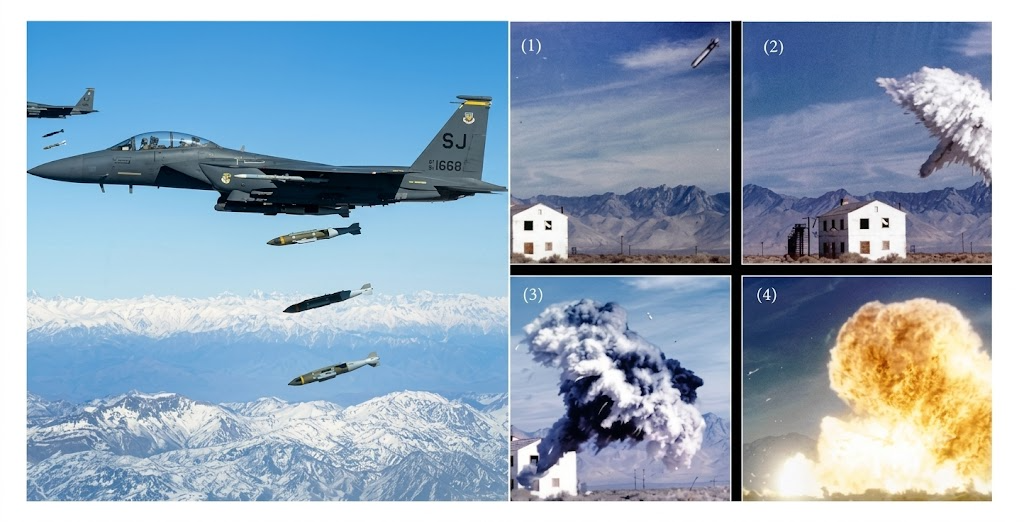
\includegraphics[width=0.7\textwidth]{image/cd15_image1.png}
\end{center}
\figcaption{1}{Hai giai đoạn phát nổ của bom nhiệt áp. (1) Bom bay gần đến mục tiêu (2) (3) Lõi trung tâm phát tán tạo thành đám mây nhiên liệu và oxygen (4) Đám mây nhiên liệu phát nổ.}

\vspace{6pt}

[7] \textbf{Đặc điểm của vụ nổ nhiệt áp:}

\begin{itemize}[leftmargin=2em, itemsep=2pt]
\item[\textcolor{accentBlue}{\textbf{--}}] Tạo quả cầu lửa lớn với nhiệt độ cực cao (2500--3000°C)
\item[\textcolor{accentBlue}{\textbf{--}}] Tạo sóng xung kích mạnh với áp suất cao lan tỏa theo mọi hướng
\item[\textcolor{accentBlue}{\textbf{--}}] Trong không gian kín, áp suất có thể đạt 29 lần áp suất khí quyển
\item[\textcolor{accentBlue}{\textbf{--}}] Sóng xung kích lan truyền với tốc độ khoảng 3,2 km/giây
\end{itemize}

[8] So với chất nổ thông thường (HE -- High Explosive), vũ khí nhiệt áp (TBE -- Thermobaric Explosive) có đặc điểm sóng xung kích khác biệt:

\textbf{Chất nổ thông thường (HE):}
\begin{itemize}[leftmargin=2em, itemsep=2pt]
\item[\textcolor{accentBlue}{\textbf{--}}] Tạo áp suất đỉnh cao hơn nhưng trong thời gian ngắn
\item[\textcolor{accentBlue}{\textbf{--}}] Pha áp suất âm xuất hiện sớm và ngắn
\item[\textcolor{accentBlue}{\textbf{--}}] Tổng năng lượng tác động thấp hơn
\end{itemize}

\textbf{Vũ khí nhiệt áp (TBE):}
\begin{itemize}[leftmargin=2em, itemsep=2pt]
\item[\textcolor{accentBlue}{\textbf{--}}] Áp suất đỉnh thấp hơn nhưng kéo dài hơn nhiều (``longer pulse duration'')
\item[\textcolor{accentBlue}{\textbf{--}}] Pha áp suất âm sâu hơn và kéo dài hơn
\item[\textcolor{accentBlue}{\textbf{--}}] Tổng năng lượng tác động lớn hơn (diện tích dưới đường cong lớn hơn)
\end{itemize}

Đặc điểm này làm cho vũ khí nhiệt áp đặc biệt nguy hiểm trong không gian kín như hầm ngầm, boongke, hoặc tòa nhà.

\begin{center}
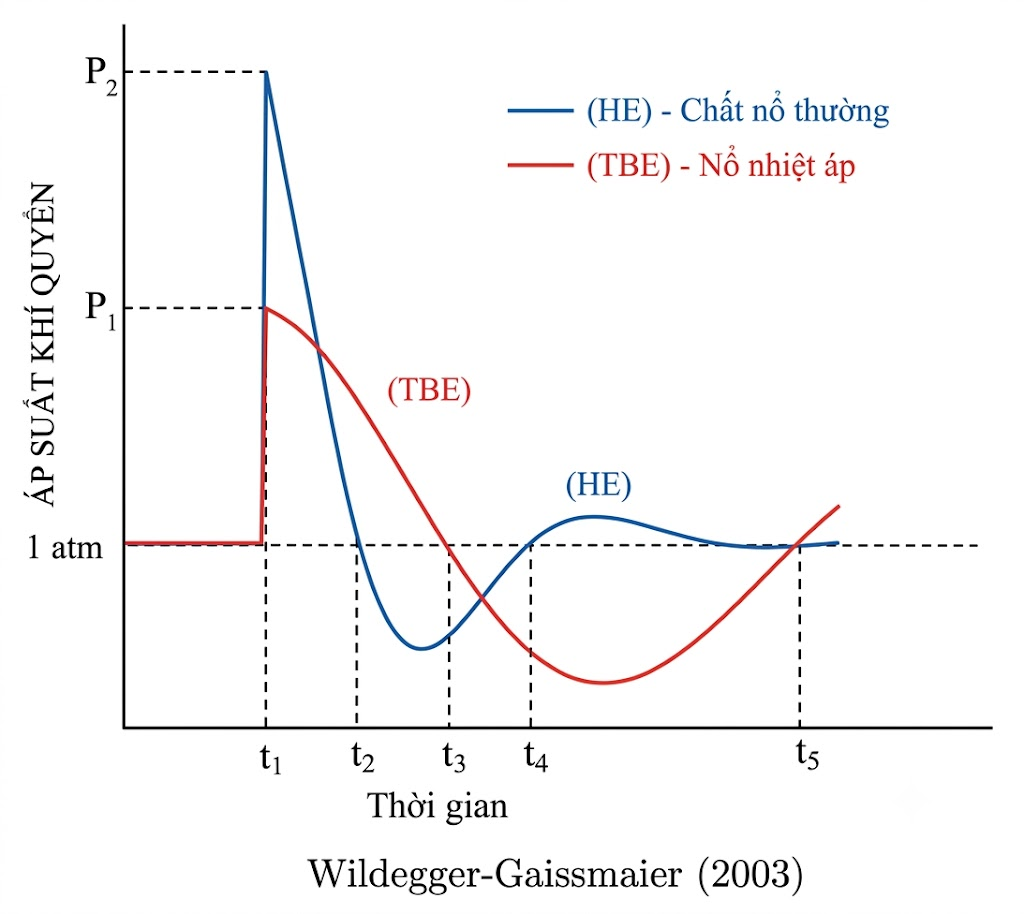
\includegraphics[width=0.6\textwidth]{image/cd15_image2.png}
\end{center}
\figcaption{2}{Thay đổi áp suất trong suốt quá trình diễn ra nổ của chất nổ thường và nổ nhiệt áp.}

\vspace{6pt}

[9] \textbf{Vũ khí nhiệt áp gây tổn thương qua nhiều cơ chế:}

\begin{itemize}[leftmargin=2em, itemsep=2pt]
\item[\textcolor{accentBlue}{\textbf{--}}] \textbf{Sóng xung kích sơ cấp:} Tổn thương các cơ quan chứa không khí (phổi, ruột, tai) do chênh lệch áp suất đột ngột
\item[\textcolor{accentBlue}{\textbf{--}}] \textbf{Hiệu ứng chân không:} Pha áp suất âm kéo dài gây vỡ mao mạch phổi, xuất huyết phổi và tử vong
\item[\textcolor{accentBlue}{\textbf{--}}] \textbf{Tổn thương nhiệt:} Nhiệt độ cực cao gây bỏng nặng
\item[\textcolor{accentBlue}{\textbf{--}}] \textbf{Ngạt thở:} Tiêu thụ oxygen trong không khí, đặc biệt trong không gian kín
\item[\textcolor{accentBlue}{\textbf{--}}] \textbf{Mảnh vỡ thứ cấp:} Các mảnh vỡ từ công trình, vật liệu bị phá hủy
\end{itemize}

Đặc biệt nguy hiểm là chấn thương phổi do sóng áp suất âm sau pha áp suất dương, không đơn thuần do thiếu oxygen như nhiều người lầm tưởng.

\begin{center}
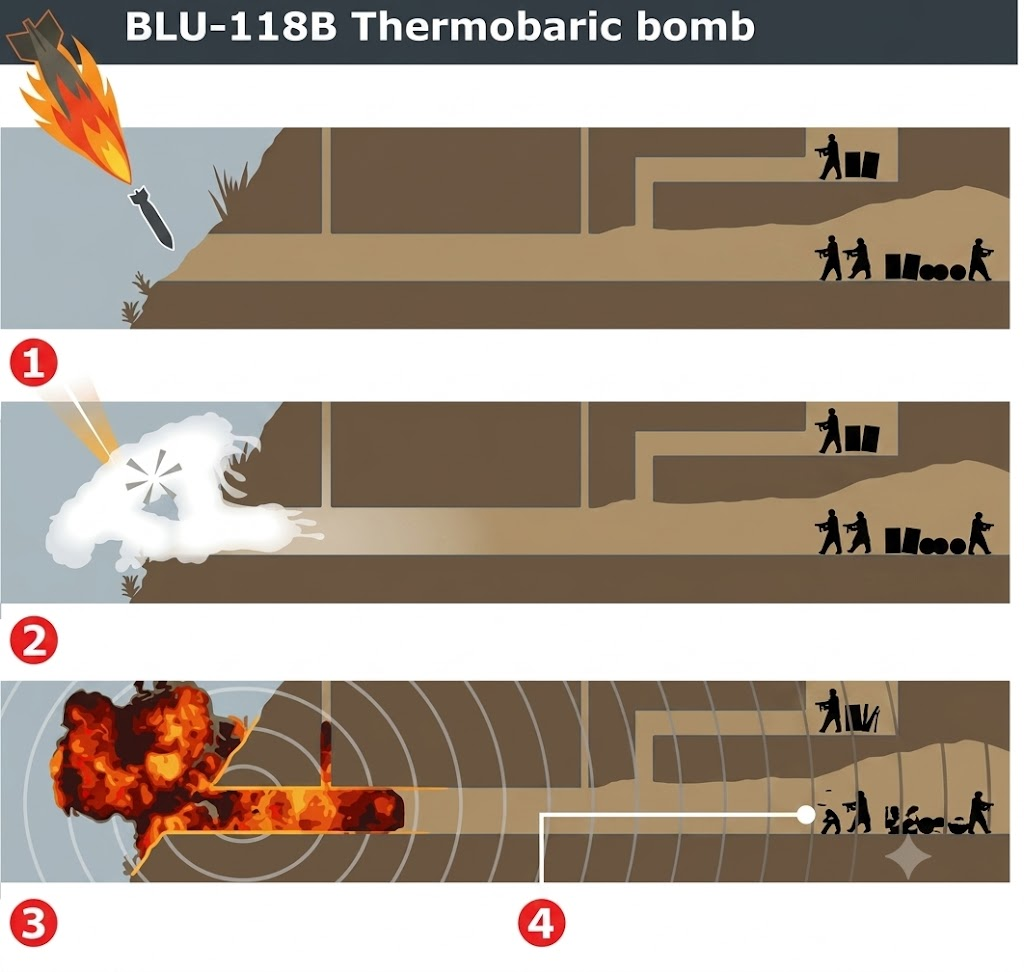
\includegraphics[width=0.7\textwidth]{image/cd15_image3.png}
\end{center}
\figcaption{3}{BLU-118B -- Cơ chế hoạt động của bom nhiệt áp với chức năng tấn công hang động. (1) Bom bay đến cửa hang động (2) Nổ sơ cấp phát tán nhiên liệu (3) Nổ chính (4) Sóng xung kích gây tổn hại binh lính ở sâu trong hang động.}

\vspace{6pt}

[10] Mặc dù có sức công phá lớn, vũ khí nhiệt áp cũng có những hạn chế:

\begin{itemize}[leftmargin=2em, itemsep=2pt]
\item[\textcolor{accentBlue}{\textbf{--}}] \textbf{Phụ thuộc vào môi trường:} Không hiệu quả trong môi trường thiếu oxygen như dưới nước hoặc không khí loãng
\item[\textcolor{accentBlue}{\textbf{--}}] \textbf{Hiệu quả hạn chế ở không gian mở:} Sức công phá giảm đáng kể khi sử dụng ở khu vực rộng, không gian mở
\item[\textcolor{accentBlue}{\textbf{--}}] \textbf{Ảnh hưởng bởi điều kiện thời tiết:} Mưa, độ ẩm cao, gió mạnh có thể làm giảm hiệu quả phân tán nhiên liệu
\item[\textcolor{accentBlue}{\textbf{--}}] \textbf{Yêu cầu kỹ thuật cao:} Cần độ chính xác trong tỷ lệ nhiên liệu và thời gian kích nổ
\item[\textcolor{accentBlue}{\textbf{--}}] \textbf{Vấn đề đạo đức:} Gây tổn thương nghiêm trọng, kéo dài, khó ngăn chặn đối với con người
\end{itemize}

[11] Trên chiến trường hiện đại, vũ khí nhiệt áp đã xuất hiện với nhiều hình thái tàn khốc: từ RPO-A Shmel của Nga (1984) được sử dụng tại Afghanistan và Chechnya, TOS-1 ``Buratino'' phóng đạn nhiệt áp hàng loạt gây hủy diệt trên diện rộng, đến FOAB ``Cha của mọi loại bom'' với sức công phá 44 tấn TNT; phía Mỹ với BLU-73/B, BLU-96/B và MOAB ``Mẹ của mọi loại bom'' từng sử dụng tại Afghanistan năm 2017; kể cả các nước khác như Trung Quốc với bom nhiệt áp hàng không và Israel với GBU-28... Sức mạnh hủy diệt kinh hoàng của những vũ khí này, với khả năng gây tổn thương đặc biệt nghiêm trọng cho con người thông qua sóng xung kích, nhiệt độ cực cao và hiệu ứng chân không, là minh chứng cho sự phi nhân tính của chiến tranh hiện đại. Thay vì tiếp tục phát triển những công cụ hủy diệt, nhân loại cần hướng đến giải pháp ngoại giao, đối thoại và hợp tác để xây dựng một thế giới hòa bình, nơi nguồn lực và trí tuệ được dành cho phát triển và cải thiện cuộc sống thay vì tạo ra những phương tiện hủy diệt nhau.

\vspace{6pt}

\hfill\textbf{Nguồn: Thầy Đào Anh Phúc biên soạn}

\end{readingpassage}
\vspace{2pt}

% === Câu 1: Trắc nghiệm ===
\question[Trắc nghiệm]{Điểm khác biệt cơ bản của vũ khí nhiệt áp so với chất nổ thông thường là gì?}
\par\vspace{4pt}
\noindent\hangindent=2.2em\hangafter=1\choiceitem{A}{Vũ khí nhiệt áp tạo ra nhiệt độ cao hơn chất nổ thông thường.}\par\vspace{4pt}
\noindent\hangindent=2.2em\hangafter=1\choiceitem{B}{Vũ khí nhiệt áp tạo ra áp suất lớn hơn chất nổ thông thường.}\par\vspace{4pt}
\noindent\hangindent=2.2em\hangafter=1\choiceitem{C}{Vũ khí nhiệt áp sử dụng oxygen trong không khí làm chất oxy hóa.}\par\vspace{4pt}
\noindent\hangindent=2.2em\hangafter=1\choiceitem{D}{Vũ khí nhiệt áp tạo ra sóng xung kích nhanh hơn chất nổ thông thường.}\par\vspace{4pt}

% === Câu 2: Trắc nghiệm ===
\question[Trắc nghiệm]{Nhiệt độ có thể đạt được trong vụ nổ nhiệt áp là bao nhiêu?}
\par\vspace{4pt}
\noindent\choiceitem{A}{1000--1500°C.}\hfill\choiceitem{B}{1500--2000°C.}\hfill\choiceitem{C}{2000--2500°C.}\hfill\choiceitem{D}{2500--3000°C.}\par\vspace{4pt}

% === Câu 3: Trắc nghiệm ===
\question[Trắc nghiệm]{Tốc độ lan truyền của sóng xung kích trong vụ nổ nhiệt áp khoảng bao nhiêu?}
\par\vspace{4pt}
\noindent\choiceitem{A}{1,2 km/giây.}\hfill\choiceitem{B}{2,2 km/giây.}\hfill\choiceitem{C}{3,2 km/giây.}\hfill\choiceitem{D}{4,2 km/giây.}\par\vspace{4pt}

% === Câu 4: Trắc nghiệm ===
\question[Trắc nghiệm]{Vật liệu nào sau đây KHÔNG phải là thành phần thường gặp trong vũ khí nhiệt áp?}
\par\vspace{4pt}
\noindent\choiceitem{A}{Bột nhôm (Al).}\hfill\choiceitem{B}{Bột magie (Mg).}\hfill\choiceitem{C}{Ethylene oxide (C\textsubscript{2}H\textsubscript{4}O).}\hfill\choiceitem{D}{Lưu huỳnh (S).}\par\vspace{4pt}

% === Câu 5: Đúng/Sai ===
\question[Đúng/Sai]{Dựa vào bài đọc, những phát biểu nào sau đây là đúng hay sai khi nói về thành phần của vũ khí nhiệt áp?}

\truefalsehead
\truefalseitem{Bột nhôm (Al) được sử dụng vì tạo ra nhiệt lượng cao khi cháy.}
\truefalseitem{Ethylene oxide (C\textsubscript{2}H\textsubscript{4}O) giúp tạo đám mây dễ khuếch tán.}
\truefalseitem{Polymer kết dính làm tăng tốc độ phản ứng cháy.}
\truefalseitem{Chất nổ sơ cấp chiếm khối lượng chính trong vũ khí nhiệt áp.}
\truefalseitem{Bột magie (Mg) khi cháy giải phóng năng lượng cực lớn.}
\truefalseend

% === Câu 6: Trắc nghiệm ===
\question[Trắc nghiệm]{Tại sao vũ khí nhiệt áp đặc biệt hiệu quả trong không gian kín?}
\par\vspace{4pt}
\noindent\hangindent=2.2em\hangafter=1\choiceitem{A}{Không gian kín giúp tăng tốc độ lan truyền của sóng xung kích.}\par\vspace{4pt}
\noindent\hangindent=2.2em\hangafter=1\choiceitem{B}{Áp suất có thể tăng lên đến 29 lần áp suất khí quyển trong không gian kín.}\par\vspace{4pt}
\noindent\hangindent=2.2em\hangafter=1\choiceitem{C}{Nhiệt độ trong không gian kín cao hơn do hiệu ứng nhà kính.}\par\vspace{4pt}
\noindent\hangindent=2.2em\hangafter=1\choiceitem{D}{Vũ khí nhiệt áp chứa các thành phần đặc biệt phá hủy bê tông.}\par\vspace{4pt}

% === Câu 7: Trắc nghiệm ===
\question[Trắc nghiệm]{Phản ứng cháy của bột nhôm trong vũ khí nhiệt áp giải phóng bao nhiêu năng lượng?}
\par\vspace{4pt}
\noindent\choiceitem{A}{1350 kJ.}\hfill\choiceitem{B}{2350 kJ.}\hfill\choiceitem{C}{3350 kJ.}\hfill\choiceitem{D}{4350 kJ.}

% === Câu 8: Ghép đôi ===
\question[Ghép đôi]{Ghép đôi giữa các giai đoạn hoạt động của vũ khí nhiệt áp với thứ tự diễn ra tương ứng. Sắp xếp các giai đoạn theo đúng trình tự từ khi bắt đầu đến khi kết thúc.}

\vspace{6pt}
\setstretch{1.3}

\textit{Cột B:}
\vspace{-6pt}
\par\vspace{4pt}
\noindent\choiceitem{A}{Thứ tự 1.}\hspace{1.2em}\choiceitem{B}{Thứ tự 2.}\hspace{1.2em}\choiceitem{C}{Thứ tự 3.}\hspace{1.2em}\choiceitem{D}{Thứ tự 4.}\hspace{1.2em}\choiceitem{E}{Thứ tự 5.}\par\vspace{3pt}
\noindent\choiceitem{F}{Thứ tự 6.}\hspace{1.2em}\choiceitem{G}{Thứ tự 7.}\hspace{1.2em}\choiceitem{H}{Thứ tự 8.}\hspace{1.2em}\choiceitem{I}{Thứ tự 9.}\par\vspace{4pt}

\vspace{6pt}

\renewcommand{\arraystretch}{1.6}
{\small\setstretch{1.0}
\begin{longtable}{|>{\raggedright\arraybackslash}m{0.55\textwidth}|>{\centering\arraybackslash}m{0.28\textwidth}|}
\hline
\rowcolor{primaryBlue!12}
\multicolumn{1}{|c|}{\cellcolor{primaryBlue!12}\textbf{Cột A}} & \cellcolor{primaryBlue!12}\textbf{Cột B} \\
\hline
\endfirsthead
\hline
\rowcolor{primaryBlue!12}
\multicolumn{1}{|c|}{\cellcolor{primaryBlue!12}\textbf{Cột A}} & \cellcolor{primaryBlue!12}\textbf{Cột B} \\
\hline
\endhead
1. Đám mây nhiên liệu phát nổ, tạo quả cầu lửa với nhiệt độ cực cao. & \dropbox[2.5cm] \\
\hline
2. Vũ khí nhiệt áp tiếp cận mục tiêu. & \dropbox[2.5cm] \\
\hline
3. Nhiên liệu trộn lẫn với oxygen trong không khí. & \dropbox[2.5cm] \\
\hline
4. Xuất hiện pha áp suất âm (hiệu ứng chân không). & \dropbox[2.5cm] \\
\hline
5. Lõi trung tâm chứa chất nổ mạnh kích hoạt. & \dropbox[2.5cm] \\
\hline
6. Sóng xung kích lan truyền với tốc độ khoảng 3,2 km/giây. & \dropbox[2.5cm] \\
\hline
7. Phân tán nhiên liệu thành đám mây hạt mịn trong không khí. & \dropbox[2.5cm] \\
\hline
8. Áp suất tăng cao, đặc biệt trong không gian kín. & \dropbox[2.5cm] \\
\hline
9. Gây sát thương qua nhiều cơ chế khác nhau. & \dropbox[2.5cm] \\
\hline
\end{longtable}
}

% === Câu 9: Đúng/Sai ===
\question[Đúng/Sai]{Dựa vào bài đọc, những phát biểu nào sau đây là đúng hay sai khi nói về sự khác biệt giữa chất nổ thông thường (HE -- High Explosive) và vũ khí nhiệt áp (TBE -- Thermobaric Explosive)?}

\truefalsehead
\truefalseitem{Vũ khí nhiệt áp tạo áp suất đỉnh cao hơn so với chất nổ thông thường.}
\truefalseitem{Pha áp suất âm của vũ khí nhiệt áp kéo dài hơn so với chất nổ thông thường.}
\truefalseitem{Chất nổ thông thường tạo tổng năng lượng tác động lớn hơn vũ khí nhiệt áp.}
\truefalseitem{Vũ khí nhiệt áp phụ thuộc vào oxygen trong không khí, còn chất nổ thông thường không.}
\truefalseitem{Thời gian tác động của vũ khí nhiệt áp ngắn hơn so với chất nổ thông thường.}
\truefalseitem{Pha áp suất âm của vũ khí nhiệt áp sâu hơn so với chất nổ thông thường.}
\truefalseitem{Cả chất nổ thông thường và vũ khí nhiệt áp đều tạo ra sóng xung kích với tốc độ như nhau.}
\truefalseitem{Vũ khí nhiệt áp có hiệu quả cao hơn chất nổ thông thường trong không gian kín.}
\truefalseend

% === Câu 10: Đúng/Sai ===
\question[Đúng/Sai]{Dựa vào bài đọc, những phát biểu nào sau đây là đúng hay sai khi nói về cơ chế gây sát thương của vũ khí nhiệt áp?}

\truefalsehead
\truefalseitem{Nguyên nhân chính gây tổn thương phổi là do giảm nồng độ oxygen.}
\truefalseitem{Sóng xung kích sơ cấp gây tổn thương các cơ quan chứa không khí.}
\truefalseitem{Hiệu ứng chân không gây vỡ mao mạch phổi.}
\truefalseitem{Mảnh vỡ thứ cấp là nguyên nhân gây tử vong chính.}
\truefalseitem{Nhiệt độ cao gây bỏng nặng cho nạn nhân.}
\truefalseitem{Pha áp suất âm kéo dài là nguyên nhân gây xuất huyết phổi.}
\truefalseend

% === Câu 11: Chọn nhiều đáp án ===
\question[Chọn nhiều đáp án]{Những yếu tố nào làm giảm hiệu quả của vũ khí nhiệt áp?}
\par\vspace{4pt}
\noindent\hangindent=2.2em\hangafter=1\choiceitemBox{A}{Môi trường thiếu oxygen.}\par\vspace{4pt}
\noindent\hangindent=2.2em\hangafter=1\choiceitemBox{B}{Không gian mở rộng.}\par\vspace{4pt}
\noindent\hangindent=2.2em\hangafter=1\choiceitemBox{C}{Mưa và độ ẩm cao.}\par\vspace{4pt}
\noindent\hangindent=2.2em\hangafter=1\choiceitemBox{D}{Ánh sáng mặt trời.}\par\vspace{4pt}
\noindent\hangindent=2.2em\hangafter=1\choiceitemBox{E}{Gió mạnh.}\par\vspace{4pt}

% === Câu 12: Ghép đôi ===
\question[Ghép đôi]{Ghép đôi giữa nguyên nhân và tác động gây sát thương tương ứng.}

\vspace{6pt}
\setstretch{1.3}

\textit{Cột B:}
\vspace{-6pt}
\par\vspace{4pt}
\noindent\hangindent=2.2em\hangafter=1\choiceitemBox{A}{Gây bỏng nặng cho nạn nhân.}\par\vspace{4pt}
\noindent\hangindent=2.2em\hangafter=1\choiceitemBox{B}{Tổn thương các cơ quan chứa không khí.}\par\vspace{4pt}
\noindent\hangindent=2.2em\hangafter=1\choiceitemBox{C}{Gây vỡ mao mạch phổi và xuất huyết.}\par\vspace{4pt}
\noindent\hangindent=2.2em\hangafter=1\choiceitemBox{D}{Tạo ra các mảnh vỡ thứ cấp.}\par\vspace{4pt}
\noindent\hangindent=2.2em\hangafter=1\choiceitemBox{E}{Gây ngạt thở trong không gian kín.}\par\vspace{4pt}

\vspace{6pt}

\renewcommand{\arraystretch}{1.6}
{\small\setstretch{1.0}
\begin{longtable}{|>{\raggedright\arraybackslash}m{0.55\textwidth}|>{\centering\arraybackslash}m{0.28\textwidth}|}
\hline
\rowcolor{primaryBlue!12}
\multicolumn{1}{|c|}{\cellcolor{primaryBlue!12}\textbf{Cột A}} & \cellcolor{primaryBlue!12}\textbf{Cột B} \\
\hline
\endfirsthead
\hline
\rowcolor{primaryBlue!12}
\multicolumn{1}{|c|}{\cellcolor{primaryBlue!12}\textbf{Cột A}} & \cellcolor{primaryBlue!12}\textbf{Cột B} \\
\hline
\endhead
1. Sóng xung kích sơ cấp. & \dropbox[2.5cm] \\
\hline
2. Pha áp suất âm kéo dài. & \dropbox[2.5cm] \\
\hline
3. Nhiệt độ cực cao. & \dropbox[2.5cm] \\
\hline
4. Tiêu thụ oxygen trong không khí. & \dropbox[2.5cm] \\
\hline
5. Phá hủy công trình, vật liệu. & \dropbox[2.5cm] \\
\hline
\end{longtable}
}

% === Câu 13: Chọn nhiều đáp án ===
\question[Chọn nhiều đáp án]{Vũ khí nhiệt áp được thiết kế để tấn công những mục tiêu nào?}
\par\vspace{4pt}
\noindent\hangindent=2.2em\hangafter=1\choiceitemBox{A}{Hầm ngầm và boongke.}\par\vspace{4pt}
\noindent\hangindent=2.2em\hangafter=1\choiceitemBox{B}{Công trình kiên cố.}\par\vspace{4pt}
\noindent\hangindent=2.2em\hangafter=1\choiceitemBox{C}{Xe tăng và thiết giáp.}\par\vspace{4pt}
\noindent\hangindent=2.2em\hangafter=1\choiceitemBox{D}{Hang động và đường hầm.}\par\vspace{4pt}
\noindent\hangindent=2.2em\hangafter=1\choiceitemBox{E}{Tàu ngầm dưới nước.}\par\vspace{4pt}
\noindent\hangindent=2.2em\hangafter=1\choiceitemBox{F}{Máy bay trên không.}\par\vspace{4pt}

% ============================================================
% CHỦ ĐỀ 13: HEMOGLOBIN -- VẬN CHUYỂN OXYGEN TRONG MÁU
% ============================================================
\newpage
\setcounter{qcounter}{0}

\phantomsection\label{b1_cd13}
\begin{topicbox}{\large CHỦ ĐỀ 13: HEMOGLOBIN -- VẬN CHUYỂN OXYGEN TRONG MÁU}
\vspace{8pt}
\textit{Đọc đoạn văn sau và trả lời các câu hỏi.}
\end{topicbox}
\vspace{5pt}
\begin{readingpassage}[]

\setstretch{1.3}

Hemoglobin là protein quan trọng nhất trong vận chuyển oxygen, có cấu tạo gồm 4 chuỗi globin (2$\alpha$, 2$\beta$) và 4 nhóm heme. Mỗi nhóm heme chứa ion Fe\textsuperscript{2+} ở trung tâm vòng porphyrin, cho phép liên kết thuận nghịch với một phân tử oxygen, liên kết này giống như một cái ``kẹp tạm thời'' gắn oxygen, không phải là phản ứng oxi hóa khử. Chức năng chính của hemoglobin bao gồm vận chuyển oxygen từ phổi đến các mô, vận chuyển một phần CO\textsubscript{2} từ mô về phổi dưới dạng HbCO\textsubscript{2}, và tham gia đệm pH để duy trì cân bằng acid-base trong máu.

\begin{center}
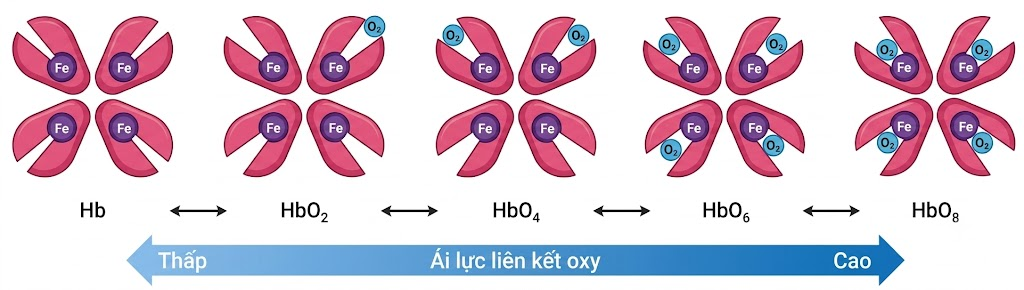
\includegraphics[width=0.55\textwidth]{image/cd13_image1.png}
\end{center}
\figcaption{1}{Quá trình liên kết oxygen của hemoglobin.}

Cơ chế liên kết với oxygen tuân theo phương trình: $\text{Hb} + 4\text{O}_2 \rightleftharpoons \text{Hb}(\text{O}_2)_4$, trong đó deoxyhemoglobin kết hợp thuận nghịch với oxygen tạo thành oxyhemoglobin. Quá trình này có tính hợp tác đặc biệt: khi một nhóm heme liên kết với phân tử oxygen đầu tiên, nó làm tăng ái lực của ba nhóm heme còn lại với oxygen (hình 1).

Dựa vào đường cong bão hòa hemoglobin (hình 2), độ bão hòa oxygen thay đổi theo vị trí trong hệ tuần hoàn, tại mao mạch phổi với PO\textsubscript{2} = 100 mmHg, độ bão hòa oxygen đạt 97--98\% cho phép hemoglobin gần như bão hòa hoàn toàn để vận chuyển oxygen tối đa đến các mô. Sau khi trao đổi khí ở mô, tại tĩnh mạch PO\textsubscript{2} giảm xuống 40 mmHg và độ bão hòa oxygen chỉ còn khoảng 75\%, cho thấy khoảng 25\% oxygen đã được giải phóng để cung cấp cho hoạt động tế bào.

\begin{center}
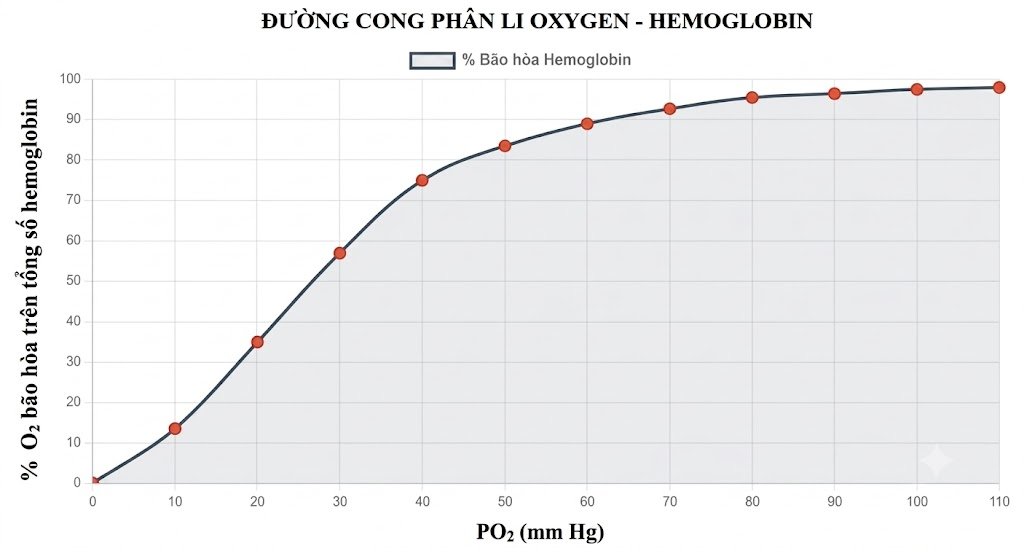
\includegraphics[width=0.65\textwidth]{image/cd13_image2.png}
\end{center}
\figcaption{2}{Đường cong bão hòa Oxy-Hemoglobin ở người tại các mức phân áp oxygen.}

Việc chỉ giải phóng 25\% oxygen ở điều kiện nghỉ ngơi thể hiện một sự thích nghi sinh lý quan trọng của cơ thể, vì lượng 25\% này tương đương khoảng 5ml O\textsubscript{2} trên 100ml máu và với lưu lượng tim 5L/phút sẽ cung cấp 250ml oxygen mỗi phút -- đủ đáp ứng nhu cầu oxygen cơ bản của cơ thể lúc nghỉ ngơi, đồng thời 75\% oxygen còn lại đóng vai trò dự trữ an toàn quan trọng sẵn sàng được huy động khi cơ thể cần thiết.

Khi hoạt động mạnh, PO\textsubscript{2} ở mô có thể giảm xuống 15--20 mmHg làm độ bão hòa hemoglobin giảm còn 30--40\%, cho phép giải phóng 60--70\% tổng lượng oxygen. Lượng CO\textsubscript{2} tăng, pH giảm dẫn đến giảm ái lực của hemoglobin với oxygen, đường cong dịch sang phải làm tăng thêm 10--15\% khả năng giải phóng oxygen, đảm bảo cung cấp oxygen linh hoạt và hiệu quả theo từng mức độ hoạt động khác nhau của cơ thể.

\hfill\textbf{Nguồn: Thầy Đào Anh Phúc biên soạn}

\end{readingpassage}
\vspace{2pt}

% === Câu 1: Trắc nghiệm ===
\question[Trắc nghiệm]{Theo văn bản, cấu trúc của hemoglobin bao gồm những thành phần nào?}
\par\vspace{4pt}
\noindent\hangindent=2.2em\hangafter=1\choiceitem{A}{2 chuỗi globin và 2 nhóm heme chứa ion Fe\textsuperscript{3+}.}\par\vspace{4pt}
\noindent\hangindent=2.2em\hangafter=1\choiceitem{B}{3 chuỗi globin và 4 nhóm heme chứa ion Fe\textsuperscript{2+}.}\par\vspace{4pt}
\noindent\hangindent=2.2em\hangafter=1\choiceitem{C}{4 chuỗi globin (2$\alpha$, 2$\beta$) và 4 nhóm heme chứa ion Fe\textsuperscript{2+}.}\par\vspace{4pt}
\noindent\hangindent=2.2em\hangafter=1\choiceitem{D}{4 chuỗi globin và 6 nhóm heme chứa ion Fe\textsuperscript{3+}.}\par\vspace{4pt}

% === Câu 2: Trắc nghiệm ===
\question[Trắc nghiệm]{Sự khác biệt chính giữa deoxyhemoglobin và oxyhemoglobin là gì?}
\par\vspace{4pt}
\noindent\hangindent=2.2em\hangafter=1\choiceitem{A}{Số lượng chuỗi globin khác nhau.}\par\vspace{4pt}
\noindent\hangindent=2.2em\hangafter=1\choiceitem{B}{Loại ion sắt trong nhóm heme khác nhau.}\par\vspace{4pt}
\noindent\hangindent=2.2em\hangafter=1\choiceitem{C}{Trạng thái liên kết với oxygen khác nhau.}\par\vspace{4pt}
\noindent\hangindent=2.2em\hangafter=1\choiceitem{D}{Cấu trúc nhóm porphyrin khác nhau.}\par\vspace{4pt}

% === Câu 3: Trắc nghiệm ===
\question[Trắc nghiệm]{Phương trình hóa học nào sau đây mô tả đúng cơ chế liên kết oxygen của một hemoglobin?}
\par\vspace{4pt}
\noindent\hangindent=2.2em\hangafter=1\choiceitem{A}{$\text{Hb} + \text{O}_2 \rightleftharpoons \text{HbO}_2$}\par\vspace{4pt}
\noindent\hangindent=2.2em\hangafter=1\choiceitem{B}{$\text{Hb} + 2\text{O}_2 \rightleftharpoons \text{Hb}(\text{O}_2)_2$}\par\vspace{4pt}
\noindent\hangindent=2.2em\hangafter=1\choiceitem{C}{$\text{Hb} + 3\text{O}_2 \rightleftharpoons \text{Hb}(\text{O}_2)_3$}\par\vspace{4pt}
\noindent\hangindent=2.2em\hangafter=1\choiceitem{D}{$\text{Hb} + 4\text{O}_2 \rightleftharpoons \text{Hb}(\text{O}_2)_4$}\par\vspace{4pt}

% === Câu 4: Đúng/Sai ===
\question[Đúng/Sai]{Dựa vào văn bản, những phát biểu nào sau đây là đúng hay sai khi nói về chức năng của hemoglobin?}

\truefalsehead
\truefalseitem{Vận chuyển O\textsubscript{2} từ phổi đến các mô.}
\truefalseitem{Vận chuyển CO\textsubscript{2} từ mô về phổi dưới dạng HbCO\textsubscript{3}.}
\truefalseitem{Tham gia đệm pH để duy trì cân bằng acid-base.}
\truefalseitem{Ion Fe thay đổi hóa trị khi liên kết với O\textsubscript{2}.}
\truefalseend

% === Câu 5: Trắc nghiệm ===
\question[Trắc nghiệm]{Vai trò của ion Fe\textsuperscript{2+} trong nhóm heme là gì?}
\par\vspace{4pt}
\noindent\hangindent=2.2em\hangafter=1\choiceitem{A}{Tạo liên kết yếu thuận nghịch với 4 phân tử O\textsubscript{2}.}\par\vspace{4pt}
\noindent\hangindent=2.2em\hangafter=1\choiceitem{B}{Tạo liên kết thuận nghịch với một phân tử O\textsubscript{2}.}\par\vspace{4pt}
\noindent\hangindent=2.2em\hangafter=1\choiceitem{C}{Xúc tác cho quá trình phân hủy oxygen thành nước.}\par\vspace{4pt}
\noindent\hangindent=2.2em\hangafter=1\choiceitem{D}{Duy trì cấu trúc bền vững của chuỗi globin.}\par\vspace{4pt}

% === Câu 6: Trắc nghiệm ===
\question[Trắc nghiệm]{Với lưu lượng tim 5L/phút và tỷ lệ giải phóng oxygen 25\% ở trạng thái nghỉ ngơi, lượng oxygen được cung cấp cho cơ thể mỗi phút là bao nhiêu?}
\par\vspace{4pt}
\noindent\choiceitem{A}{125ml}\hfill\choiceitem{B}{200ml}\hfill\choiceitem{C}{250ml}\hfill\choiceitem{D}{300ml}

% === Câu 7: Trắc nghiệm ===
\question[Trắc nghiệm]{Theo đường cong phân áp hemoglobin, tại sao cơ thể chỉ giải phóng 25\% oxygen ở điều kiện nghỉ ngơi?}
\par\vspace{4pt}
\noindent\hangindent=2.2em\hangafter=1\choiceitem{A}{Do hemoglobin có ái lực quá cao với oxygen nên khó giải phóng.}\par\vspace{4pt}
\noindent\hangindent=2.2em\hangafter=1\choiceitem{B}{Để duy trì dự trữ an toàn 75\% oxygen sẵn sàng huy động khi cần thiết.}\par\vspace{4pt}
\noindent\hangindent=2.2em\hangafter=1\choiceitem{C}{Vì các mô chỉ cần một lượng oxygen rất nhỏ để hoạt động bình thường.}\par\vspace{4pt}
\noindent\hangindent=2.2em\hangafter=1\choiceitem{D}{Do PO\textsubscript{2} ở tĩnh mạch quá cao làm hemoglobin không thể giải phóng nhiều oxygen.}\par\vspace{4pt}

% === Câu 8: Đúng/Sai ===
\question[Đúng/Sai]{Những phát biểu nào sau đây là đúng khi nói về sự thay đổi đường cong hemoglobin và các chỉ số sinh lý máu khi hoạt động thể chất mạnh?}

\truefalsehead
\truefalseitem{Đường cong dịch chuyển sang phải.}
\truefalseitem{Khả năng giải phóng oxygen tăng thêm 10--15\%.}
\truefalseitem{Lượng CO\textsubscript{2} tăng làm giảm ái lực hemoglobin với oxygen.}
\truefalseitem{pH tăng do tích tụ CO\textsubscript{2}.}
\truefalseitem{Cho phép giải phóng 60--70\% tổng lượng oxygen.}
\truefalseend

% === Câu 9: Ghép đôi ===
\question[Ghép đôi]{Ghép đôi giữa điều kiện sinh lý với mức độ bão hòa oxygen của hemoglobin tương ứng:}

\vspace{6pt}
\setstretch{1.3}

\textit{Cột B:}
\vspace{-6pt}
\par\vspace{4pt}
\noindent\hangindent=2.2em\hangafter=1\choiceitem{A}{30--40\%.}\par\vspace{4pt}
\noindent\hangindent=2.2em\hangafter=1\choiceitem{B}{97--98\%.}\par\vspace{4pt}
\noindent\hangindent=2.2em\hangafter=1\choiceitem{C}{75\%.}\par\vspace{4pt}

\vspace{6pt}

\renewcommand{\arraystretch}{1.6}
{\small\setstretch{1.0}
\begin{longtable}{|>{\raggedright\arraybackslash}m{0.55\textwidth}|>{\centering\arraybackslash}m{0.28\textwidth}|}
\hline
\rowcolor{primaryBlue!12}
\multicolumn{1}{|c|}{\cellcolor{primaryBlue!12}\textbf{Cột A}} & \cellcolor{primaryBlue!12}\textbf{Cột B} \\
\hline
\endfirsthead
\hline
\rowcolor{primaryBlue!12}
\multicolumn{1}{|c|}{\cellcolor{primaryBlue!12}\textbf{Cột A}} & \cellcolor{primaryBlue!12}\textbf{Cột B} \\
\hline
\endhead
1. Mao mạch phổi (PO\textsubscript{2} = 100 mmHg). & \dropbox[2.5cm] \\
\hline
2. Tĩnh mạch lúc nghỉ ngơi (PO\textsubscript{2} = 40 mmHg). & \dropbox[2.5cm] \\
\hline
3. Hoạt động mạnh (PO\textsubscript{2} = 15--20 mmHg). & \dropbox[2.5cm] \\
\hline
\end{longtable}
}

% === Câu 10: Điền khuyết ===
\question[Điền khuyết]{Điền các cụm từ thích hợp (không quá 2 tiếng) vào chỗ trống để hoàn thành đoạn văn tổng hợp nội dung bài đọc:}

\vspace{4pt}
\setstretch{1.4}
Cơ chế liên kết oxygen của hemoglobin có tính hợp tác đặc biệt, khi một (1)\,\dropbox[2cm] liên kết với O\textsubscript{2} đầu tiên sẽ làm tăng (2)\,\dropbox[2cm] của ba nhóm heme còn lại với oxygen. Tại (3)\,\dropbox[2cm] phổi với PO\textsubscript{2} = 100 mmHg, độ (4)\,\dropbox[2cm] O\textsubscript{2} đạt 97--98\% cho phép vận chuyển oxygen tối đa đến các mô.

% ============================================================
% CHỦ ĐỀ 14: VẬN CHUYỂN CO₂ TRONG MÁU
% ============================================================
\newpage
\setcounter{qcounter}{0}

\phantomsection\label{b1_cd14}
\begin{topicbox}{\large CHỦ ĐỀ 14: VẬN CHUYỂN CO\textsubscript{2} TRONG MÁU}
\vspace{8pt}
\textit{Đọc đoạn văn sau và trả lời các câu hỏi.}
\end{topicbox}
\vspace{5pt}
\begin{readingpassage}[]

\setstretch{1.3}

[1] Carbon dioxide (CO\textsubscript{2}) được tạo ra từ quá trình trao đổi chất tế bào phải được vận chuyển từ các mô đến phổi để thải ra ngoài. Khác với oxygen, CO\textsubscript{2} được vận chuyển trong máu thông qua ba cơ chế khác nhau, mỗi cơ chế đóng góp tỷ lệ phần trăm khác nhau vào tổng lượng CO\textsubscript{2} được vận chuyển.

[2] \textbf{Cơ chế 1: Hòa tan trực tiếp.} Một phần nhỏ CO\textsubscript{2} hòa tan trực tiếp trong huyết tương (lượng hòa tan tuân thủ theo định luật Henry về áp suất riêng phần). Đây là hình thức vận chuyển CO\textsubscript{2} đơn giản nhất.

[3] \textbf{Cơ chế 2: Tạo thành bicarbonate} (Hình 1). Phần lớn CO\textsubscript{2} trải qua phản ứng với nước diễn ra bên trong hồng cầu để phân li thành các ion:

\vspace{2pt}
\begin{center}
$\text{CO}_2 + \text{H}_2\text{O} \rightleftharpoons \text{H}_2\text{CO}_3 \rightleftharpoons \text{HCO}_3^- + \text{H}^+$
\end{center}
\vspace{2pt}

[4] Phản ứng này được xúc tác bởi enzyme carbonic anhydrase. Đa phần ion H\textsuperscript{+} được hemoglobin đệm (liên kết), trong khi các ion HCO\textsubscript{3}\textsuperscript{-} khuếch tán vào huyết tương thông qua trao đổi với ion Cl\textsuperscript{-}.

[5] \textbf{Cơ chế 3: Hợp chất carbamino.} CO\textsubscript{2} có thể gắn trực tiếp vào các nhóm amino trên phần globin của hemoglobin (không phải nhóm heme):

\vspace{2pt}
\begin{center}
$\text{CO}_2 + \text{Hb-NH}_2 \rightleftharpoons \text{Hb-NHCOO}^- + \text{H}^+$
\end{center}
\vspace{2pt}

[6] Phản ứng này không cần enzyme và có thể đảo ngược.

[7] Đồng thời Hemoglobin khử oxy (deoxyhemoglobin) có ái lực với CO\textsubscript{2} lớn hơn oxyhemoglobin (hiệu ứng Haldane), giúp thuận lợi cho việc nhận CO\textsubscript{2} tại mô và thải CO\textsubscript{2} tại phổi.

\begin{center}
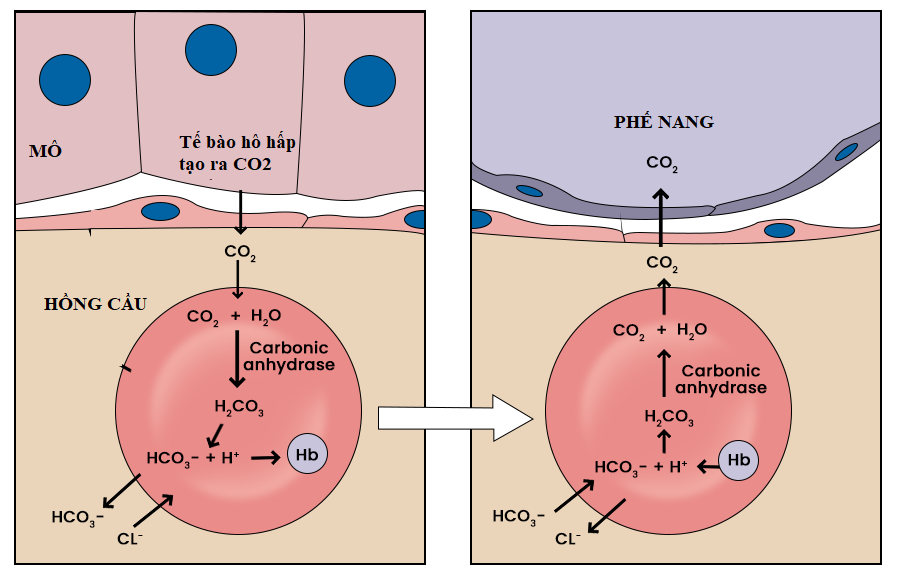
\includegraphics[width=0.55\textwidth]{image/cd12_image1.png}
\end{center}
\figcaption{1}{Cơ chế trao đổi CO\textsubscript{2} thông qua con đường tạo bicarbonate.}

\vspace{6pt}

\tablecaption{1}{Các cơ chế vận chuyển CO\textsubscript{2} và tỉ lệ phần trăm.}

\renewcommand{\arraystretch}{1.4}
{\small
\setstretch{1.0}%
\begin{tabular}{|>{\raggedright\arraybackslash}m{0.30\textwidth}|>{\centering\arraybackslash}m{0.20\textwidth}|>{\raggedright\arraybackslash}m{0.34\textwidth}|}
\hline
\rowcolor{primaryBlue!12}
\textbf{Phương thức vận chuyển} & \textbf{Tỷ lệ \% tổng CO\textsubscript{2}} & \textbf{Vị trí gắn kết} \\
\hline
Hòa tan trực tiếp & 7\% & Huyết tương \\
\hline
Tạo thành bicarbonate & 70\% & Hồng cầu $\rightarrow$ huyết tương \\
\hline
Hợp chất carbamino & 23\% & Chuỗi globin của hemoglobin \\
\hline
\end{tabular}
}

\vspace{6pt}

\tablecaption{2}{So sánh các thông số của O\textsubscript{2} và CO\textsubscript{2} tại mô và tại mao mạch phổi.}

\renewcommand{\arraystretch}{1.4}
{\small
\setstretch{1.0}%
\begin{tabular}{|>{\raggedright\arraybackslash}m{0.34\textwidth}|>{\centering\arraybackslash}m{0.24\textwidth}|>{\centering\arraybackslash}m{0.24\textwidth}|}
\hline
\rowcolor{primaryBlue!12}
\textbf{Thông số} & \textbf{Tại các mô} & \textbf{Tại mao mạch phổi} \\
\hline
Áp suất riêng phần CO\textsubscript{2} (PCO\textsubscript{2}) & Cao (45--50 mmHg) & Thấp (35--40 mmHg) \\
\hline
Áp suất riêng phần O\textsubscript{2} (PO\textsubscript{2}) & Thấp (30--40 mmHg) & Cao (95--100 mmHg) \\
\hline
pH & Thấp hơn (acid hơn) & Cao hơn (ít acid hơn) \\
\hline
Độ bão hòa oxy của hemoglobin & Thấp (75\%) & Cao (98\%) \\
\hline
Nạp/Thải CO\textsubscript{2} & Nạp CO\textsubscript{2} & Thải CO\textsubscript{2} \\
\hline
Dạng hemoglobin chủ yếu & Deoxyhemoglobin & Oxyhemoglobin \\
\hline
\end{tabular}
}

\vspace{6pt}

\hfill\textbf{Nguồn: Thầy Đào Anh Phúc biên soạn}

\end{readingpassage}
\vspace{2pt}

% === Câu 1: Trắc nghiệm ===
\question[Trắc nghiệm]{Dựa vào đoạn văn, carbonic anhydrase cần thiết cho:}
\par\vspace{4pt}
\noindent\hangindent=2.2em\hangafter=1\choiceitem{A}{Hòa tan CO\textsubscript{2} trực tiếp.}\par\vspace{4pt}
\noindent\hangindent=2.2em\hangafter=1\choiceitem{B}{Tạo thành bicarbonate.}\par\vspace{4pt}
\noindent\hangindent=2.2em\hangafter=1\choiceitem{C}{Tạo thành hợp chất carbamino.}\par\vspace{4pt}
\noindent\hangindent=2.2em\hangafter=1\choiceitem{D}{Cả ba cơ chế vận chuyển.}\par\vspace{4pt}

% === Câu 2: Trắc nghiệm ===
\question[Trắc nghiệm]{CO\textsubscript{2} gắn với hemoglobin tại vị trí nào?}
\par\vspace{4pt}
\noindent\hangindent=2.2em\hangafter=1\choiceitem{A}{Nhóm heme chứa Fe như oxygen.}\par\vspace{4pt}
\noindent\hangindent=2.2em\hangafter=1\choiceitem{B}{Khoang trung tâm của phân tử hemoglobin.}\par\vspace{4pt}
\noindent\hangindent=2.2em\hangafter=1\choiceitem{C}{Các nhóm amino trên chuỗi globin.}\par\vspace{4pt}
\noindent\hangindent=2.2em\hangafter=1\choiceitem{D}{Bề mặt ngoài của màng hồng cầu.}\par\vspace{4pt}

% === Câu 3: Ghép đôi ===
\question[Ghép đôi]{Ghép đôi giữa cơ chế vận chuyển với tỷ lệ phần trăm tương ứng.}

\vspace{6pt}
\setstretch{1.3}

\textit{Cột B:}
\vspace{-6pt}
\par\vspace{4pt}
\noindent\hangindent=2.2em\hangafter=1\choiceitem{A}{23\%.}\par\vspace{4pt}
\noindent\hangindent=2.2em\hangafter=1\choiceitem{B}{7\%.}\par\vspace{4pt}
\noindent\hangindent=2.2em\hangafter=1\choiceitem{C}{70\%.}\par\vspace{4pt}

\vspace{6pt}

\renewcommand{\arraystretch}{1.6}
{\small\setstretch{1.0}
\begin{longtable}{|>{\raggedright\arraybackslash}m{0.55\textwidth}|>{\centering\arraybackslash}m{0.28\textwidth}|}
\hline
\rowcolor{primaryBlue!12}
\multicolumn{1}{|c|}{\cellcolor{primaryBlue!12}\textbf{Cột A}} & \cellcolor{primaryBlue!12}\textbf{Cột B} \\
\hline
\endfirsthead
\hline
\rowcolor{primaryBlue!12}
\multicolumn{1}{|c|}{\cellcolor{primaryBlue!12}\textbf{Cột A}} & \cellcolor{primaryBlue!12}\textbf{Cột B} \\
\hline
\endhead
1. Hòa tan trực tiếp. & \dropbox[2.5cm] \\
\hline
2. Tạo thành bicarbonate. & \dropbox[2.5cm] \\
\hline
3. Hợp chất carbamino. & \dropbox[2.5cm] \\
\hline
\end{longtable}
}

% === Câu 4: Trắc nghiệm ===
\question[Trắc nghiệm]{Phản ứng $\text{CO}_2 + \text{H}_2\text{O} \rightleftharpoons \text{H}_2\text{CO}_3 \rightleftharpoons \text{HCO}_3^- + \text{H}^+$ diễn ra chủ yếu ở đâu?}
\par\vspace{4pt}
\noindent\hangindent=2.2em\hangafter=1\choiceitem{A}{Trong huyết tương.}\par\vspace{4pt}
\noindent\hangindent=2.2em\hangafter=1\choiceitem{B}{Bên trong hồng cầu.}\par\vspace{4pt}
\noindent\hangindent=2.2em\hangafter=1\choiceitem{C}{Tại màng tế bào của các mô.}\par\vspace{4pt}
\noindent\hangindent=2.2em\hangafter=1\choiceitem{D}{Trong khoang kẽ giữa các tế bào.}\par\vspace{4pt}

% === Câu 5: Chọn nhiều đáp án ===
\question[Chọn nhiều đáp án]{Dựa vào bảng 2, những đặc điểm nào sau đây đúng khi nói về điều kiện tại mô?}
\par\vspace{4pt}
\noindent\hangindent=2.2em\hangafter=1\choiceitemBox{A}{Áp suất riêng phần CO\textsubscript{2} cao hơn so với phổi.}\par\vspace{4pt}
\noindent\hangindent=2.2em\hangafter=1\choiceitemBox{B}{Áp suất riêng phần O\textsubscript{2} thấp hơn so với phổi.}\par\vspace{4pt}
\noindent\hangindent=2.2em\hangafter=1\choiceitemBox{C}{Độ pH cao hơn so với phổi.}\par\vspace{4pt}
\noindent\hangindent=2.2em\hangafter=1\choiceitemBox{D}{Độ bão hòa oxy của hemoglobin thấp hơn.}\par\vspace{4pt}
\noindent\hangindent=2.2em\hangafter=1\choiceitemBox{E}{Hemoglobin chủ yếu ở dạng oxyhemoglobin.}\par\vspace{4pt}
\noindent\hangindent=2.2em\hangafter=1\choiceitemBox{F}{Quá trình chính là nạp CO\textsubscript{2} vào máu.}\par\vspace{4pt}

% === Câu 6: Đúng/Sai ===
\question[Đúng/Sai]{Dựa vào đoạn văn, những phát biểu nào sau đây là đúng hay sai khi nói về các cơ chế vận chuyển CO\textsubscript{2}?}

\truefalsehead
\truefalseitem{Hòa tan trực tiếp là cơ chế đơn giản nhất.}
\truefalseitem{Phản ứng tạo carbamino cần enzyme xúc tác.}
\truefalseitem{Ion bicarbonate khuếch tán vào huyết tương.}
\truefalseitem{Hemoglobin đệm ion H\textsuperscript{+} trong phản ứng bicarbonate.}
\truefalseitem{Định luật Henry áp dụng cho cơ chế hòa tan trực tiếp.}
\truefalseend

% === Câu 7: Kéo thả ===
\question[Kéo thả]{Kéo thả từ vào ô trống phù hợp để hoàn thành đoạn văn:}
\vspace{-4pt}
\dragitems{
\centering
    \dragitem{huyết tương} \dragitem{carbonic anhydrase} \dragitem{ba cơ chế}\\[1pt]
    \dragitem{hemoglobin} \dragitem{hồng cầu} \dragitem{bicarbonate}\\[1pt]
    \dragitem{mô} \dragitem{phổi} \dragitem{amino}
}

\setstretch{1.4}
Carbon dioxide được tạo ra tại (1)\,\dropbox[2cm] phải được vận chuyển đến (2)\,\dropbox[2cm] để thải ra ngoài. Quá trình này diễn ra thông qua (3)\,\dropbox[2cm] khác nhau. Cơ chế chính là tạo thành (4)\,\dropbox[2cm] bên trong (5)\,\dropbox[2cm] với sự xúc tác của enzyme (6)\,\dropbox[2cm]. CO\textsubscript{2} cũng có thể gắn trực tiếp vào các nhóm (7)\,\dropbox[2cm] trên chuỗi globin của (8)\,\dropbox[2cm] hoặc hòa tan trong (9)\,\dropbox[2cm].

% === Câu 8: Trắc nghiệm ===
\question[Trắc nghiệm]{Hiệu ứng Haldane mô tả hiện tượng nào sau đây?}
\par\vspace{4pt}
\noindent\hangindent=2.2em\hangafter=1\choiceitem{A}{CO\textsubscript{2} làm tăng ái lực của hemoglobin với oxygen.}\par\vspace{4pt}
\noindent\hangindent=2.2em\hangafter=1\choiceitem{B}{Deoxyhemoglobin có ái lực CO\textsubscript{2} lớn hơn oxyhemoglobin.}\par\vspace{4pt}
\noindent\hangindent=2.2em\hangafter=1\choiceitem{C}{Carbonic anhydrase hoạt động mạnh hơn tại phổi.}\par\vspace{4pt}
\noindent\hangindent=2.2em\hangafter=1\choiceitem{D}{CO\textsubscript{2} hòa tan tốt hơn trong môi trường có pH thấp.}\par\vspace{4pt}

% === Câu 9: Trắc nghiệm ===
\question[Trắc nghiệm]{Tại sao CO\textsubscript{2} tích tụ tại mô lại làm giảm pH?}
\par\vspace{4pt}
\noindent\hangindent=2.2em\hangafter=1\choiceitem{A}{CO\textsubscript{2} trực tiếp là một acid mạnh.}\par\vspace{4pt}
\noindent\hangindent=2.2em\hangafter=1\choiceitem{B}{CO\textsubscript{2} phản ứng với protein tạo acid.}\par\vspace{4pt}
\noindent\hangindent=2.2em\hangafter=1\choiceitem{C}{CO\textsubscript{2} tạo thành H\textsubscript{2}CO\textsubscript{3} rồi phân ly H\textsuperscript{+}.}\par\vspace{4pt}
\noindent\hangindent=2.2em\hangafter=1\choiceitem{D}{CO\textsubscript{2} ức chế hoạt động của hệ đệm.}\par\vspace{4pt}

% === Câu 10: Ghép đôi ===
\question[Ghép đôi]{Ghép đôi giữa thông số sinh lý với giá trị tại mô tương ứng.}

\vspace{6pt}
\setstretch{1.3}

\textit{Cột B:}
\vspace{-6pt}
\par\vspace{4pt}
\noindent\hangindent=2.2em\hangafter=1\choiceitem{A}{30--40.}\par\vspace{4pt}
\noindent\hangindent=2.2em\hangafter=1\choiceitem{B}{75\%.}\par\vspace{4pt}
\noindent\hangindent=2.2em\hangafter=1\choiceitem{C}{45--50.}\par\vspace{4pt}
\noindent\hangindent=2.2em\hangafter=1\choiceitem{D}{Deoxyhemoglobin.}\par\vspace{4pt}

\vspace{6pt}

\renewcommand{\arraystretch}{1.6}
{\small\setstretch{1.0}
\begin{longtable}{|>{\raggedright\arraybackslash}m{0.55\textwidth}|>{\centering\arraybackslash}m{0.28\textwidth}|}
\hline
\rowcolor{primaryBlue!12}
\multicolumn{1}{|c|}{\cellcolor{primaryBlue!12}\textbf{Cột A}} & \cellcolor{primaryBlue!12}\textbf{Cột B} \\
\hline
\endfirsthead
\hline
\rowcolor{primaryBlue!12}
\multicolumn{1}{|c|}{\cellcolor{primaryBlue!12}\textbf{Cột A}} & \cellcolor{primaryBlue!12}\textbf{Cột B} \\
\hline
\endhead
1. PCO\textsubscript{2} (mmHg). & \dropbox[2.5cm] \\
\hline
2. PO\textsubscript{2} (mmHg). & \dropbox[2.5cm] \\
\hline
3. Độ bão hòa oxy. & \dropbox[2.5cm] \\
\hline
4. Dạng hemoglobin chủ yếu. & \dropbox[2.5cm] \\
\hline
\end{longtable}
}

% ============================================================
% CHỦ ĐỀ 15: PHẢN ỨNG NỔ 
% ─────────────────────────────────────────────────────────────
\newpage
\setcounter{qcounter}{0}

\phantomsection\label{b1_cd15}
\begin{topicbox}{\large CHỦ ĐỀ 15: NHIỆT ĐỘNG LỰC HỌC VÀ ĐỘNG HÓA HỌC PHẢN ỨNG NỔ}
\vspace{8pt}
\textit{Đọc đoạn văn sau và trả lời các câu hỏi.}
\vspace{6pt}
\end{topicbox}
\vspace{5pt}

\begin{readingpassage}[]
\setstretch{1.3}

[1] Quá trình phân hủy của thuốc nổ hóa học về bản chất là một phản ứng oxy hóa -- khử tỏa nhiệt cực mạnh diễn ra với vận tốc cực cao. Tuy nhiên, cần phân biệt rõ hai trạng thái diễn biến hoàn toàn khác nhau: Cháy bùng (Deflagration) và Nổ sóng kích động (Detonation). Cháy bùng là quá trình cháy lan truyền qua khối chất nổ với vận tốc dưới âm ($v < 1000$\,m/s), cơ chế truyền năng lượng chủ yếu dựa vào truyền nhiệt và khuếch tán phân tử. Ngược lại, nổ sóng kích động lan truyền với vận tốc siêu thanh (1000 -- 9000\,m/s), trong đó một sóng nén cơ học cực mạnh (sóng kích động) nén ép và kích hoạt phản ứng hóa học của khối chất nổ gần như tức thời.

[2] Một đặc tính cốt lõi của thuốc nổ hóa học là nguyên lý Oxy hóa tự thân (Self-Oxidation). Khác với phản ứng cháy thông thường cần lấy oxygen từ không khí, phân tử thuốc nổ tích hợp đồng thời các nhóm chức chứa oxygen (chất oxy hóa, như --NO\textsubscript{2}, --ONO\textsubscript{2}) và các nguyên tố giàu năng lượng (nhiên liệu, như C, H) trên cùng một khung phân tử. Mức độ thừa hay thiếu oxygen được đo bằng chỉ số Cân bằng Oxygen (Oxygen Balance -- OB\%):

\vspace{4pt}
\begin{center}
$\text{OB\%} = \left[\dfrac{-16 \times (2x + y/2 - z)}{M}\right] \times 100\%$
\end{center}
\vspace{2pt}

\textit{(Trong đó $x$, $y$, $z$ lần lượt là số nguyên tử C, H, O trong công thức C\textsubscript{x}H\textsubscript{y}N\textsubscript{w}O\textsubscript{z} và $M$ là khối lượng phân tử.)}

[3] Về mặt định lượng, OB\% cho biết khối lượng oxygen (tính bằng gam) còn thừa hoặc còn thiếu trên mỗi 100\,g chất nổ để oxy hóa hoàn toàn nhiên liệu thành CO\textsubscript{2} và H\textsubscript{2}O: giá trị âm ứng với thiếu oxygen, giá trị dương ứng với thừa oxygen.

[4] Về mặt năng lượng, các phân tử thuốc nổ chứa những liên kết kém bền như N--O và C--N (năng lượng liên kết chỉ vào khoảng 200 -- 300\,kJ/mol). Khi phản ứng nổ xảy ra, các liên kết này bị đứt gãy và các nguyên tử nitrogen nhanh chóng tái hợp thành khí N\textsubscript{2}. Liên kết ba N$\equiv$N có năng lượng liên kết cực lớn (945\,kJ/mol); chính sự chênh lệch năng lượng khổng lồ giữa trạng thái liên kết ban đầu và sản phẩm N\textsubscript{2} siêu bền vững là nguồn gốc phát tán nhiệt nổ ($Q_{ex}$) và giải phóng thể tích khí nổ ($V_0$) tạo ra áp suất sóng nổ ($P_{det} \propto \rho \cdot V_d^2$).

[5] Để đánh giá sức mạnh công phá và độ an toàn vận hành, các kỹ sư dựa vào vận tốc nổ ($V_d$), nhiệt nổ ($Q_{ex}$), thể tích khí ($V_0$), nhiệt độ phân hủy ($T_{dec}$) và đặc biệt là Độ nhạy va đập ($E_{imp}$) -- công cơ học/năng lượng rơi tối thiểu, tính bằng Joule (J), cần thiết để làm khối chất nổ bắt đầu phát nổ.

\vspace{6pt}
\tablecaption{1}{So sánh thông số nhiệt động học và kỹ thuật của một số chất nổ đơn chất.}
\renewcommand{\arraystretch}{1.4}
{\small
\setstretch{1.0}%
\begin{center}
\begin{tabular}{|>{\centering\arraybackslash}m{2.2cm}|>{\centering\arraybackslash}m{2.2cm}|>{\centering\arraybackslash}m{1.2cm}|>{\centering\arraybackslash}m{1.2cm}|>{\centering\arraybackslash}m{1.2cm}|>{\centering\arraybackslash}m{1.2cm}|>{\centering\arraybackslash}m{1.2cm}|>{\centering\arraybackslash}m{1.2cm}|}
\hline
\rowcolor{primaryBlue!12}
\textbf{Chất nổ} & \textbf{Công thức} & \textbf{OB (\%)} & \textbf{$V_d$ (m/s)} & \textbf{$Q_{ex}$ (kJ/kg)} & \textbf{$V_0$ (L/kg)} & \textbf{$E_{imp}$ (J)} & \textbf{$T_{dec}$ (°C)} \\
\hline
TNT & C\textsubscript{7}H\textsubscript{5}N\textsubscript{3}O\textsubscript{6} & $-74{,}0$ & 6900 & 4200 & 730 & 15,0 & 295 \\
\hline
RDX & C\textsubscript{3}H\textsubscript{6}N\textsubscript{6}O\textsubscript{6} & $-21{,}6$ & 8750 & 5540 & 900 & 7,5 & 210 \\
\hline
PETN & C\textsubscript{5}H\textsubscript{8}N\textsubscript{4}O\textsubscript{12} & $-10{,}1$ & 8400 & 5790 & 780 & 3,0 & 190 \\
\hline
Nitroglycerin & C\textsubscript{3}H\textsubscript{5}N\textsubscript{3}O\textsubscript{9} & $+3{,}5$ & 7700 & 6300 & 782 & 0,2 & 160 \\
\hline
\end{tabular}
\end{center}
}

\hfill\textbf{Nguồn: Thầy Đào Anh Phúc biên soạn}
\end{readingpassage}
\vspace{2pt}

% === Câu 1: Trắc nghiệm ===
\question[Trắc nghiệm]{Sự khác biệt bản chất nhất về cơ chế truyền năng lượng giữa cháy bùng (deflagration) và nổ sóng kích động (detonation) của vật liệu nổ là gì?}
\par\vspace{4pt}
\noindent\hangindent=2.2em\hangafter=1\choiceitem{A}{Cháy bùng sinh ra nhiệt lượng lớn hơn rất nhiều so với quá trình nổ sóng kích động.}\par\vspace{4pt}
\noindent\hangindent=2.2em\hangafter=1\choiceitem{B}{Cháy bùng bắt buộc cần oxygen không khí, còn nổ sóng kích động chỉ dùng oxygen tự thân.}\par\vspace{4pt}
\noindent\hangindent=2.2em\hangafter=1\choiceitem{C}{Cháy bùng lan truyền nhờ truyền nhiệt và khuếch tán, còn nổ lan truyền nhờ sóng nén siêu thanh.}\par\vspace{4pt}
\noindent\hangindent=2.2em\hangafter=1\choiceitem{D}{Cháy bùng không tạo ra sản phẩm thể khí, trong khi quá trình nổ sinh ra lượng khí khổng lồ.}\par\vspace{4pt}

% === Câu 2: Ghép đôi ===
\question[Ghép đôi]{Ghép mỗi thông số đặc tính của chất nổ (Cột A) với ý nghĩa vật lý -- hóa học tương ứng (Cột B):}
\vspace{6pt}
\setstretch{1.3}

\textit{Cột B:}
\vspace{-6pt}
\par\vspace{4pt}
\noindent\hangindent=2.2em\hangafter=1\choiceitem{A}{Năng lượng cơ học tối thiểu cần tác động để kích hoạt phản ứng nổ.}\par\vspace{4pt}
\noindent\hangindent=2.2em\hangafter=1\choiceitem{B}{Vận tốc truyền của sóng nén cơ học xuyên qua khối chất nổ.}\par\vspace{4pt}
\noindent\hangindent=2.2em\hangafter=1\choiceitem{C}{Lượng nhiệt giải phóng khi 1\,kg chất nổ phân hủy hoàn toàn.}\par\vspace{4pt}
\noindent\hangindent=2.2em\hangafter=1\choiceitem{D}{Mức độ thừa hoặc thiếu oxygen để oxy hóa hoàn toàn C và H.}\par\vspace{4pt}
\noindent\hangindent=2.2em\hangafter=1\choiceitem{E}{Nhiệt độ tối thiểu khiến khối chất nổ tự bùng cháy.}\par\vspace{4pt}
\vspace{6pt}

\renewcommand{\arraystretch}{1.6}
{\small\setstretch{1.0}
\begin{longtable}{|>{\raggedright\arraybackslash}m{0.44\textwidth}|>{\centering\arraybackslash}m{0.44\textwidth}|}
\hline
\rowcolor{primaryBlue!12}
\multicolumn{1}{|c|}{\cellcolor{primaryBlue!12}\textbf{Cột A}} & \cellcolor{primaryBlue!12}\textbf{Cột B} \\
\hline
\endfirsthead
\hline
\rowcolor{primaryBlue!12}
\multicolumn{1}{|c|}{\cellcolor{primaryBlue!12}\textbf{Cột A}} & \cellcolor{primaryBlue!12}\textbf{Cột B} \\
\hline
\endhead
1. Nhiệt nổ ($Q_{ex}$) & \dropbox[2.5cm] \\
\hline
2. Độ nhạy va đập ($E_{imp}$) & \dropbox[2.5cm] \\
\hline
3. Cân bằng Oxygen (OB\%) & \dropbox[2.5cm] \\
\hline
4. Vận tốc nổ ($V_d$) & \dropbox[2.5cm] \\
\hline
\end{longtable}
}

% === Câu 3: Trắc nghiệm ===
\question[Trắc nghiệm]{Vì sao các hợp chất nổ mạnh thường tích hợp nhóm chức chứa nitrogen (--NO\textsubscript{2}, --ONO\textsubscript{2}) trong phân tử, mặc dù sự tạo thành liên kết N$\equiv$N ở sản phẩm mới là nguồn giải phóng năng lượng chính?}
\par\vspace{4pt}
\noindent\hangindent=2.2em\hangafter=1\choiceitem{A}{Vì các liên kết kém bền chứa nitrogen dễ đứt gãy để chuyển thành N\textsubscript{2} có năng lượng liên kết cực bền.}\par\vspace{4pt}
\noindent\hangindent=2.2em\hangafter=1\choiceitem{B}{Vì nitrogen hoạt động như chất xúc tác, làm giảm năng lượng hoạt hóa cho phản ứng giữa carbon và oxygen.}\par\vspace{4pt}
\noindent\hangindent=2.2em\hangafter=1\choiceitem{C}{Vì nitrogen đóng vai trò chất oxy hóa chính, cung cấp toàn bộ electron cho carbon và hydrogen.}\par\vspace{4pt}
\noindent\hangindent=2.2em\hangafter=1\choiceitem{D}{Vì khí N\textsubscript{2} sinh ra có thể tích giãn nở lớn gấp nhiều lần các khí CO\textsubscript{2} và H\textsubscript{2}O.}\par\vspace{4pt}

% === Câu 4: Điền khuyết ===
\question[Điền khuyết]{Điền số thích hợp (làm tròn đến hàng đơn vị) vào chỗ trống:}
\vspace{5pt}
\setstretch{1.4}
\begin{itemize}[leftmargin=*, itemsep=5pt, topsep=0pt, partopsep=0pt, parsep=0pt, label=\textcolor{primaryBlue}{\textbullet}]
\item Xét 1,0\,kg TNT có OB $= -74{,}0$\%. Để oxy hóa hoàn toàn phần nhiên liệu còn thiếu trong 1,0\,kg TNT thành CO\textsubscript{2} và H\textsubscript{2}O, cần bổ sung thêm một lượng oxygen từ bên ngoài là (1)\,\dropbox[2cm] gram.
\item Khi 1,0\,kg Nitroglycerin phát nổ hoàn toàn, nhiệt lượng giải phóng lớn hơn so với 1,0\,kg TNT là (2)\,\dropbox[2cm] kJ.
\item Xét chỉ số an toàn va đập, năng lượng tối thiểu để kích nổ mẫu TNT lớn gấp (3)\,\dropbox[2cm] lần so với mẫu PETN.
\end{itemize}

% === Câu 5: Đúng/Sai ===
\question[Đúng/Sai]{Đánh giá tính Đúng/Sai của các mệnh đề liên quan đến nguyên lý Oxy hóa tự thân và chỉ số OB\%:}

\truefalsehead
\truefalseitem{Nitroglycerin có OB $= +3{,}5$\%, nghĩa là sản phẩm sau khi nổ hoàn toàn sẽ chứa một lượng khí oxygen tự do (O\textsubscript{2}).}
\truefalseitem{Thuốc nổ có OB\% càng âm sâu thì sản phẩm khí càng chứa nhiều khí độc CO và muội than (C).}
\truefalseitem{Mọi chất nổ có $V_d > 8000$\,m/s đều có chỉ số OB\% mang giá trị dương.}
\truefalseitem{Phản ứng oxy hóa tự thân giúp thuốc nổ có thể phát nổ bình thường trong chân không hoặc dưới nước sâu.}
\truefalseend

% === Câu 6: Điền khuyết ===
\question[Điền khuyết]{Trong thí nghiệm kiểm tra độ nhạy va đập, người ta thả rơi tự do một quả văng khối lượng 2,0\,kg từ độ cao $h$ (m) xuống mẫu thử RDX. Giả thiết toàn bộ thế năng của quả văng chuyển hóa hoàn toàn thành năng lượng va đập tác dụng lên mẫu thử, gia tốc trọng trường $g = 9{,}8$\,m/s\textsuperscript{2}. Xác định độ cao tối thiểu $h$ để năng lượng va đập đạt đúng ngưỡng kích nổ $E_{imp}$ của RDX. Điền số thích hợp (làm tròn đến chữ số thập phân thứ hai):}
\vspace{5pt}
\setstretch{1.4}
\begin{itemize}[leftmargin=*, itemsep=5pt, topsep=0pt, partopsep=0pt, parsep=0pt, label=\textcolor{primaryBlue}{\textbullet}]
\item Kết quả: $h =$ (1)\,\dropbox[2cm] m.
\end{itemize}

% === Câu 7: Ghép đôi ===
\question[Ghép đôi]{Phân tích dữ liệu chéo trong bảng, ghép mỗi chất nổ (Cột A) với đặc tính kỹ thuật -- ứng dụng thực tế phù hợp nhất (Cột B):}
\vspace{6pt}
\setstretch{1.3}

\textit{Cột B:}
\vspace{-6pt}
\par\vspace{4pt}
\noindent\hangindent=2.2em\hangafter=1\choiceitem{A}{Nhiệt độ phân hủy rất cao (295\,°C), độ nhạy va đập thấp (15,0\,J), rất an toàn khi đúc đạn dược nhưng hiệu suất nổ thấp nhất bảng.}\par\vspace{4pt}
\noindent\hangindent=2.2em\hangafter=1\choiceitem{B}{Vận tốc nổ cao nhất (8750\,m/s), nhiệt nổ lớn, cân bằng tốt giữa sức công phá và độ an toàn vận chuyển tương đối ($E_{imp} = 7{,}5$\,J).}\par\vspace{4pt}
\noindent\hangindent=2.2em\hangafter=1\choiceitem{C}{Độ nhạy va đập cực kỳ nguy hiểm ($E_{imp} = 0{,}2$\,J), rất dễ phát nổ do rung xóc, nhưng tỏa nhiệt nổ lớn nhất (6300\,kJ/kg).}\par\vspace{4pt}
\noindent\hangindent=2.2em\hangafter=1\choiceitem{D}{Vận tốc nổ cao (8400\,m/s) và rất nhạy va đập ($E_{imp} = 3{,}0$\,J), thích hợp làm thuốc nổ mồi hoặc dây nổ kích nổ cho chất nổ trơ.}\par\vspace{4pt}
\noindent\hangindent=2.2em\hangafter=1\choiceitem{E}{Là chất nổ duy nhất không giải phóng khí N\textsubscript{2} khi phân hủy.}\par\vspace{4pt}
\vspace{6pt}

\renewcommand{\arraystretch}{1.6}
{\small\setstretch{1.0}
\begin{longtable}{|>{\raggedright\arraybackslash}m{0.44\textwidth}|>{\centering\arraybackslash}m{0.44\textwidth}|}
\hline
\rowcolor{primaryBlue!12}
\multicolumn{1}{|c|}{\cellcolor{primaryBlue!12}\textbf{Cột A}} & \cellcolor{primaryBlue!12}\textbf{Cột B} \\
\hline
\endfirsthead
\hline
\rowcolor{primaryBlue!12}
\multicolumn{1}{|c|}{\cellcolor{primaryBlue!12}\textbf{Cột A}} & \cellcolor{primaryBlue!12}\textbf{Cột B} \\
\hline
\endhead
1. Nitroglycerin & \dropbox[2.5cm] \\
\hline
2. TNT & \dropbox[2.5cm] \\
\hline
3. PETN & \dropbox[2.5cm] \\
\hline
4. RDX & \dropbox[2.5cm] \\
\hline
\end{longtable}
}

% === Câu 8: Trắc nghiệm ===
\question[Trắc nghiệm]{Để khắc phục việc TNT thiếu oxygen trầm trọng (OB $= -74{,}0$\%) sinh khí độc CO và giảm hiệu suất nhiệt, người ta phối trộn TNT với ammonium nitrate (NH\textsubscript{4}NO\textsubscript{3}, OB $= +20{,}0$\%) tạo hỗn hợp thuốc nổ Amatol. Để hỗn hợp Amatol đạt cân bằng oxygen lý tưởng (OB\textsubscript{hh} $= 0$\%), tỷ lệ phần trăm khối lượng của TNT trong hỗn hợp gần nhất với giá trị nào?}
\par\vspace{4pt}
\noindent\choiceitem{A}{21,3\%.}\hfill\choiceitem{B}{27,0\%.}\hfill\choiceitem{C}{35,5\%.}\hfill\choiceitem{D}{78,7\%.}

% === Câu 9: Đúng/Sai ===
\question[Đúng/Sai]{Dựa trên nguyên lý nhiệt động lực học, độ nhạy $E_{imp}$ và vận tốc nổ $V_d$ trong bài, đánh giá tính Đúng/Sai của các nhận định chuyên môn sau:}

\truefalsehead
\truefalseitem{Nitroglycerin nguyên chất không được dùng trực tiếp làm thuốc nổ khai thác mỏ dân dụng vì ranh giới an toàn va đập quá thấp ($E_{imp} = 0{,}2$\,J), dễ gây kích nổ ngoài ý muốn khi vận chuyển.}
\truefalseitem{Để kích nổ một khối TNT trơ một cách tin cậy, kỹ sư có thể dùng một lượng nhỏ PETN làm ngòi nổ mồi nhờ PETN có độ nhạy va đập cao hơn và vận tốc nổ lớn hơn TNT.}
\truefalseitem{Nếu vận tốc nổ $V_d$ tăng lên 2 lần thì áp suất sóng kích động ($P_{det}$) do nó tạo ra cũng tăng đúng 2 lần (giả định khối lượng riêng $\rho$ không đổi).}
\truefalseitem{Một chất nổ đạt OB $= 0$\% luôn đảm bảo thể tích khí nổ ($V_0$) trên mỗi kg đạt giá trị lớn nhất tuyệt đối so với các chất nổ có OB $\neq 0$\%.}
\truefalseend

% === Câu 10: Kéo thả ===
\question[Kéo thả]{Kéo các cụm từ thích hợp từ Kho dữ liệu thả vào ô trống để hoàn thiện đoạn tóm tắt nội dung bài học:}
\vspace{-4pt}
\dragitems{
\centering
    \dragitem{sóng kích động} \dragitem{truyền nhiệt} \dragitem{Oxy hóa tự thân}\\[1pt]
    \dragitem{Oxygen Balance} \dragitem{N$\equiv$N} \dragitem{C--N}\\[1pt]
    \dragitem{thấp} \dragitem{cao}
}

\setstretch{1.4}
Quá trình nổ khác biệt hoàn toàn với cháy bùng ở chỗ sự lan truyền diễn ra nhờ (1)\,\dropbox[3cm] siêu thanh thay vì cơ chế (2)\,\dropbox[2.5cm]. Nhờ nguyên lý (3)\,\dropbox[3cm], thuốc nổ không phụ thuộc oxygen môi trường. Nguồn năng lượng khổng lồ của phản ứng phân hủy nổ xuất phát từ sự phá vỡ các liên kết yếu và sự hình thành liên kết ba (4)\,\dropbox[2cm] cực kỳ bền vững. Trong đánh giá an toàn kỹ thuật, chất nổ có độ nhạy va đập $E_{imp}$ càng (5)\,\dropbox[2cm] thì nguy cơ phát nổ ngoài ý muốn do va chạm cơ học càng lớn.


% ─────────────────────────────────────────────────────────────


% CHỦ ĐỀ 16: THUỐC ỨC CHẾ CẠNH TRANH ENZYME
% ============================================================
\newpage
\setcounter{qcounter}{0}

\phantomsection\label{b1_cd16}
\begin{topicbox}{\large CHỦ ĐỀ 16: THUỐC ỨC CHẾ CẠNH TRANH ENZYME}
\vspace{8pt}
\textit{Đọc đoạn văn sau và trả lời các câu hỏi.}
\end{topicbox}
\vspace{5pt}
\begin{readingpassage}[]

\setstretch{1.5}

Enzyme là các protein xúc tác sinh học, đóng vai trò sống còn trong việc đẩy nhanh các phản ứng chuyển hóa. Cơ chế xúc tác bắt đầu khi cơ chất tự nhiên (Substrate -- S) tiến vào gắn với enzyme tại vị trí đặc hiệu gọi là \textbf{trung tâm hoạt động} (Active site). Quá trình này đòi hỏi tính đặc hiệu không gian ba chiều nghiêm ngặt (mô hình ổ khóa -- chìa khóa hoặc khớp ứng động) và sự tương thích hóa lý (lực Van der Waals, liên kết hydrogen, tương tác tĩnh điện) giữa cơ chất và enzyme.

Trong thiết kế thuốc hiện đại, các nhà khoa học phát triển các \textbf{``thuốc ức chế cạnh tranh''} (Competitive inhibitors -- I). Đây là các phân tử có cấu trúc không gian ba chiều và phân bố điện tích gần giống với cơ chất tự nhiên, cho phép chúng cạnh tranh để gắn vào trung tâm hoạt động của enzyme mục tiêu. Khi thuốc đã chiếm chỗ, cơ chất tự nhiên không thể gắn vào, làm ngừng trệ chuỗi phản ứng sinh hóa của mầm bệnh.

Tuy nhiên, việc chế tạo thuốc ức chế cạnh tranh là một bài toán tối ưu hóa đa mục tiêu. Một ứng viên thuốc tiềm năng cần dung hòa ba yếu tố cốt lõi:

\textbf{1. Ái lực liên kết (Affinity):} Đánh giá qua nồng độ ức chế tối đa một nửa ($IC_{50}$ -- nồng độ thuốc cần thiết để ức chế 50\% hoạt tính enzyme). Giá trị $IC_{50}$ càng nhỏ, thuốc gắn càng chặt, hiệu quả càng cao. Tỷ lệ phần trăm enzyme bị ức chế ($Y$) ở một nồng độ thuốc $[\text{I}]$ nhất định được tính gần đúng theo công thức:

\vspace{2pt}
\begin{center}
$Y = \dfrac{[\text{I}]}{IC_{50} + [\text{I}]} \times 100\%$
\end{center}
\vspace{2pt}

\textbf{2. Tính chọn lọc (Selectivity):} Thuốc chỉ được ức chế enzyme của mầm bệnh (Enzyme X) mà không được gắn nhầm vào các enzyme của người (ví dụ: Enzyme Y), nhằm tránh độc tính. Chỉ số chọn lọc $SI$ được tính như sau; $SI$ càng lớn, thuốc càng an toàn:

\vspace{2pt}
\begin{center}
$SI = \dfrac{IC_{50}(\text{Enzyme Y})}{IC_{50}(\text{Enzyme X})}$
\end{center}
\vspace{2pt}

\textbf{3. Độ kị nước (LogP):} Đặc trưng cho mức độ kị nước của phân tử thuốc, quyết định khả năng thấm qua màng. Màng tế bào là lớp phospholipid kép; thuốc cần độ kị nước phù hợp (LogP từ 1 đến 3) để đi qua màng. Nếu kị nước quá cao (LogP > 5), thuốc sẽ bị giữ lại ở màng tế bào và không hòa tan tốt trong máu.

Trong một dự án tìm thuốc trị virus viêm gan, nhóm nghiên cứu đã tổng hợp ba ứng viên thuốc (A, B, C) ức chế enzyme Protease X của virus. Kết quả thử nghiệm in vitro (trong ống nghiệm) và đánh giá độ an toàn trên enzyme Protease Y của người được tóm tắt ở Bảng 1.

\vspace{6pt}

\tablecaption{1}{Dữ liệu thử nghiệm dược lý của ba ứng viên thuốc ức chế cạnh tranh.}
\renewcommand{\arraystretch}{1.4}
{\small
\setstretch{1.0}%
\begin{tabular}{|>{\raggedright\arraybackslash}m{0.18\textwidth}|>{\centering\arraybackslash}m{0.22\textwidth}|>{\centering\arraybackslash}m{0.22\textwidth}|>{\centering\arraybackslash}m{0.18\textwidth}|}
\hline
\rowcolor{primaryBlue!12}
\textbf{Ứng viên thuốc} & \textbf{$IC_{50}$ với Protease X của virus (nM)} & \textbf{$IC_{50}$ với Protease Y của người (nM)} & \textbf{Độ kị nước (LogP)} \\
\hline
Thuốc A & 5,0 & 50,0 & 1,8 \\
\hline
Thuốc B & 1,5 & 3,0 & 6,5 \\
\hline
Thuốc C & 20,0 & 10\,000,0 & 2,2 \\
\hline
\end{tabular}
}

\vspace{6pt}

\hfill\textbf{Nguồn: Thầy Đào Anh Phúc biên soạn}

\end{readingpassage}
\vspace{2pt}

% === Câu 1: Trắc nghiệm ===
\question[Trắc nghiệm]{Theo văn bản, cơ chế hoạt động cốt lõi của thuốc ức chế cạnh tranh là gì?}
\par\vspace{4pt}
\noindent\hangindent=2.2em\hangafter=1\choiceitem{A}{Gắn không thuận nghịch vào trung tâm hoạt động, phá hủy vĩnh viễn cấu trúc enzyme.}\par\vspace{4pt}
\noindent\hangindent=2.2em\hangafter=1\choiceitem{B}{Gắn vào trung tâm hoạt động nhờ cấu trúc tương đồng, ngăn cơ chất thật tiến vào.}\par\vspace{4pt}
\noindent\hangindent=2.2em\hangafter=1\choiceitem{C}{Gắn vào vị trí khác trên enzyme, làm biến dạng trung tâm hoạt động của enzyme.}\par\vspace{4pt}
\noindent\hangindent=2.2em\hangafter=1\choiceitem{D}{Gắn trực tiếp vào cơ chất tự nhiên, làm cơ chất bất hoạt trước khi gặp enzyme.}\par\vspace{4pt}

% === Câu 2: Đúng/Sai ===
\question[Đúng/Sai]{Dựa vào các định nghĩa trong văn bản, các mệnh đề sau đây đúng hay sai?}

\truefalsehead
\truefalseitem{Thuốc có giá trị $IC_{50}$ càng cao thì ái lực liên kết với enzyme càng mạnh.}
\truefalseitem{Tính đặc hiệu không gian ba chiều là điều kiện bắt buộc để thuốc gắn vào trung tâm hoạt động.}
\truefalseitem{Chỉ số chọn lọc ($SI$) càng lớn chứng tỏ thuốc càng ít gây tác dụng phụ cho tế bào người.}
\truefalseitem{Thuốc có độ kị nước (LogP) càng lớn thì việc lưu thông trong máu càng dễ dàng.}
\truefalseend

% === Câu 3: Trắc nghiệm ===
\question[Trắc nghiệm]{Trong một thí nghiệm đo hoạt tính, người ta cấp một lượng thuốc ức chế cạnh tranh sao cho nồng độ thuốc $[\text{I}]$ trong dung dịch duy trì chính xác bằng với giá trị $IC_{50}$ của loại thuốc đó. Dựa vào công thức đã cho, tỷ lệ phần trăm enzyme bị ức chế ($Y$) là bao nhiêu?}
\par\vspace{4pt}
\noindent\choiceitem{A}{25,0\%}\hfill\choiceitem{B}{50,0\%}\hfill\choiceitem{C}{75,0\%}\hfill\choiceitem{D}{100,0\%}

% === Câu 4: Ghép đôi ===
\question[Ghép đôi]{Trong giai đoạn ra quyết định (Trade-off), việc đánh giá tổng quan các đặc tính của thuốc là cực kỳ quan trọng. Hãy ghép tên các ứng viên thuốc (Cột A) với nhận định lâm sàng tương ứng (Cột B) dựa trên Bảng 1.}

\vspace{6pt}
\setstretch{1.3}

\textit{Cột B:}
\vspace{-6pt}
\par\vspace{4pt}
\noindent\hangindent=2.2em\hangafter=1\choiceitem{A}{Rất an toàn, độ thấm màng tốt nhưng cần dùng liều lượng lớn do ái lực với đích yếu nhất.}\par\vspace{4pt}
\noindent\hangindent=2.2em\hangafter=1\choiceitem{B}{Hiệu quả cân bằng, ái lực mạnh, dễ qua màng tế bào nhưng có nguy cơ gây độc nhẹ cho người.}\par\vspace{4pt}
\noindent\hangindent=2.2em\hangafter=1\choiceitem{C}{Có ái lực mạnh nhất với virus nhưng dễ gây ngộ độc nặng cho người và khó hòa tan trong máu do quá kị nước.}\par\vspace{4pt}
\noindent\hangindent=2.2em\hangafter=1\choiceitem{D}{Thuốc lý tưởng nhất, ái lực mạnh nhất, không gây độc tính và dễ dàng hòa tan trong mọi dung môi sinh học.}\par\vspace{4pt}

\vspace{6pt}

\renewcommand{\arraystretch}{1.6}
{\small\setstretch{1.0}
\begin{longtable}{|>{\raggedright\arraybackslash}m{0.55\textwidth}|>{\centering\arraybackslash}m{0.28\textwidth}|}
\hline
\rowcolor{primaryBlue!12}
\multicolumn{1}{|c|}{\cellcolor{primaryBlue!12}\textbf{Cột A}} & \cellcolor{primaryBlue!12}\textbf{Cột B} \\
\hline
\endfirsthead
\hline
\rowcolor{primaryBlue!12}
\multicolumn{1}{|c|}{\cellcolor{primaryBlue!12}\textbf{Cột A}} & \cellcolor{primaryBlue!12}\textbf{Cột B} \\
\hline
\endhead
1. Thuốc A. & \dropbox[2.5cm] \\
\hline
2. Thuốc B. & \dropbox[2.5cm] \\
\hline
3. Thuốc C. & \dropbox[2.5cm] \\
\hline
\end{longtable}
}

% === Câu 5: Điền khuyết ===
\question[Điền khuyết]{Một thử nghiệm lâm sàng yêu cầu nồng độ thuốc phải đủ để ức chế được 90\% số lượng enzyme Protease X của virus nhằm ngăn chặn sự nhân lên. Sử dụng công thức tính $Y$ trong bài đọc. (Điền số nguyên hoặc số thập phân. Làm tròn đến một chữ số sau dấu phẩy.)}

\vspace{4pt}
\begin{itemize}[leftmargin=2em, itemsep=4pt]
\item[$\bullet$] Để đạt được hiệu quả 90\% này, nếu sử dụng thuốc A, bác sĩ cần duy trì nồng độ thuốc A trong tế bào là \dropbox[2cm] nM.
\item[$\bullet$] Tương tự, nếu sử dụng thuốc B, nồng độ cần duy trì để đạt hiệu quả ức chế 90\% là \dropbox[2cm] nM.
\end{itemize}

% === Câu 6: Đúng/Sai ===
\question[Đúng/Sai]{Giả sử virus viêm gan đột biến gen, khiến một amino acid kị nước tại trung tâm hoạt động của Protease X bị thay thế bởi một amino acid mang điện tích âm (ưa nước). Dựa trên nguyên lý tương tác phân tử, các đánh giá sau là đúng hay sai?}

\truefalsehead
\truefalseitem{Ái lực liên kết của cả ba ứng viên thuốc (A, B, C) hiện tại với enzyme đột biến này nhiều khả năng sẽ bị suy giảm mạnh.}
\truefalseitem{Giá trị $IC_{50}$ của thuốc B đối với Protease X đột biến này sẽ giảm xuống (tức là thuốc B trở nên mạnh hơn).}
\truefalseitem{Giải pháp khắc phục hiệu quả là thiết kế lại khung thuốc bằng cách gắn thêm các nhóm chức mang điện tích dương vào vị trí tương ứng.}
\truefalseitem{Đột biến này chắc chắn sẽ làm mất đi khả năng gây bệnh của virus viêm gan đối với tế bào người.}
\truefalseend

% === Câu 7: Điền khuyết ===
\question[Điền khuyết]{Dựa vào công thức tính chỉ số chọn lọc $SI$ và các dữ liệu được cung cấp ở Bảng 1, hãy tính toán và cho biết chỉ số chọn lọc $SI$ của ứng viên Thuốc C có giá trị bằng bao nhiêu? (Điền số nguyên.)}

\vspace{4pt}
Kết quả: \dropbox[2cm]

% === Câu 8: Trắc nghiệm ===
\question[Trắc nghiệm]{Mặc dù Thuốc B có ái lực mạnh nhất với đích tác dụng (Protease X), tại sao Hội đồng khoa học lại ưu tiên đưa Thuốc A vào giai đoạn thử nghiệm trên động vật thay vì Thuốc B?}
\par\vspace{4pt}
\noindent\hangindent=2.2em\hangafter=1\choiceitem{A}{Vì Thuốc A có cấu trúc không gian phức tạp hơn, giúp đẩy nhanh quá trình tổng hợp công nghiệp.}\par\vspace{4pt}
\noindent\hangindent=2.2em\hangafter=1\choiceitem{B}{Vì Thuốc B có chỉ số $IC_{50}$ với enzyme người cao hơn Thuốc A, chứng tỏ nó an toàn hơn Thuốc A.}\par\vspace{4pt}
\noindent\hangindent=2.2em\hangafter=1\choiceitem{C}{Vì Thuốc B ức chế cả enzyme người (độc tính cao) và có LogP = 6,5 gây cản trở việc hòa tan trong máu.}\par\vspace{4pt}
\noindent\hangindent=2.2em\hangafter=1\choiceitem{D}{Vì Thuốc A có độ kị nước thấp nhất trong ba loại thuốc, nên nó hoàn toàn không thể đi qua màng tế bào của vật chủ.}\par\vspace{4pt}

% === Câu 9: Ghép đôi ===
\question[Ghép đôi]{Ghép các thông số/khái niệm (Cột A) với bản chất khoa học tương ứng mô tả tính chất của thuốc (Cột B).}

\vspace{6pt}
\setstretch{1.3}

\textit{Cột B:}
\vspace{-6pt}
\par\vspace{4pt}
\noindent\hangindent=2.2em\hangafter=1\choiceitem{A}{Đo lường ranh giới an toàn sinh học giữa việc diệt mầm bệnh và gây hại tế bào chủ.}\par\vspace{4pt}
\noindent\hangindent=2.2em\hangafter=1\choiceitem{B}{Mức độ cạnh tranh ái lực, quyết định nồng độ cần thiết để ức chế enzyme mục tiêu.}\par\vspace{4pt}
\noindent\hangindent=2.2em\hangafter=1\choiceitem{C}{Khả năng thiết lập tương tác khóa -- chìa khóa dựa trên điện tích phân tử thuốc.}\par\vspace{4pt}
\noindent\hangindent=2.2em\hangafter=1\choiceitem{D}{Khả năng hấp thu và phân bố qua hàng rào màng phospholipid của tế bào.}\par\vspace{4pt}
\noindent\hangindent=2.2em\hangafter=1\choiceitem{E}{Tính tương thích về hình dạng không gian ba chiều giữa thuốc và trung tâm hoạt động.}\par\vspace{4pt}

\vspace{6pt}

\renewcommand{\arraystretch}{1.6}
{\small\setstretch{1.0}
\begin{longtable}{|>{\raggedright\arraybackslash}m{0.55\textwidth}|>{\centering\arraybackslash}m{0.28\textwidth}|}
\hline
\rowcolor{primaryBlue!12}
\multicolumn{1}{|c|}{\cellcolor{primaryBlue!12}\textbf{Cột A}} & \cellcolor{primaryBlue!12}\textbf{Cột B} \\
\hline
\endfirsthead
\hline
\rowcolor{primaryBlue!12}
\multicolumn{1}{|c|}{\cellcolor{primaryBlue!12}\textbf{Cột A}} & \cellcolor{primaryBlue!12}\textbf{Cột B} \\
\hline
\endhead
1. Chỉ số $IC_{50}$. & \dropbox[2.5cm] \\
\hline
2. Chỉ số chọn lọc ($SI$). & \dropbox[2.5cm] \\
\hline
3. Độ kị nước (LogP). & \dropbox[2.5cm] \\
\hline
4. Mô hình ổ khóa -- chìa khóa. & \dropbox[2.5cm] \\
\hline
\end{longtable}
}

% === Câu 10: Kéo thả ===
\question[Kéo thả]{Kéo các cụm từ thích hợp vào chỗ trống để tóm tắt lý thuyết phát triển thuốc ức chế enzyme.}
\vspace{-4pt}
\dragitems{
\centering
    \dragitem{ái lực} \dragitem{chọn lọc} \dragitem{độc tính}\\[1pt]
    \dragitem{cạnh tranh} \dragitem{không gian ba chiều} \dragitem{xúc tác}
}

\setstretch{1.4}
``Các loại thuốc ức chế (1)\,\dropbox[2cm] hoạt động hiệu quả nhờ khả năng vừa khít vào trung tâm hoạt động của enzyme dựa trên sự phù hợp về mặt (2)\,\dropbox[2cm]. Một ứng viên thuốc thành công không chỉ cần có (3)\,\dropbox[2cm] liên kết mạnh với đích tác dụng nhằm tối ưu hóa hiệu quả, mà còn bắt buộc phải có tính (4)\,\dropbox[2cm] rất cao đối với đích đó để tránh gắn nhầm, từ đó ngăn ngừa nguy cơ gây ra (5)\,\dropbox[2cm] cho hệ thống sinh lý của cơ thể người.''

% CHỦ ĐỀ 17: PULSE OXIMETER
% ============================================================
\newpage
\setcounter{qcounter}{0}

\phantomsection\label{b1_cd17}
\begin{topicbox}{\large CHỦ ĐỀ 17: PULSE OXIMETER}
\vspace{8pt}
\textit{Đọc đoạn văn sau và trả lời các câu hỏi.}
\end{topicbox}
\vspace{5pt}
\begin{readingpassage}[]

\setstretch{1.5}

[1] Độ bão hòa oxygen trong máu ngoại vi (SpO\textsubscript{2}) là tỷ lệ phần trăm hemoglobin trong máu động mạch có mang oxygen so với tổng lượng hemoglobin. Chỉ số này phản ánh mức độ hiệu quả của việc vận chuyển oxy từ phổi đến các cơ quan trong cơ thể. Nhịp tim là số chu kỳ co bóp của tim trong một phút. Pulse oximeter là thiết bị y tế không xâm lấn được dùng rộng rãi để đo đồng thời SpO\textsubscript{2} và nhịp tim (Hình 1).

\begin{center}
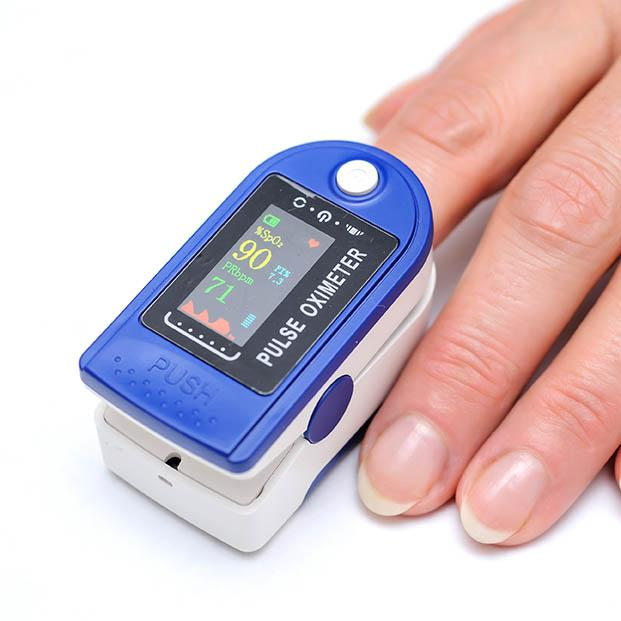
\includegraphics[width=0.35\textwidth]{image/cd16_image1.jpg}
\end{center}
\figcaption{1}{Pulse oximeter.}

\vspace{6pt}

[2] Thiết bị hoạt động dựa trên nguyên lý quang phổ hấp thụ, sử dụng hai bước sóng ánh sáng khác nhau để phân biệt hai dạng hemoglobin. Oxyhemoglobin (hemoglobin mang oxygen, ký hiệu HbO\textsubscript{2}) hấp thụ mạnh ánh sáng hồng ngoại 940 nm, còn deoxyhemoglobin (hemoglobin không mang oxygen, ký hiệu Hb) hấp thụ mạnh ánh sáng đỏ 660 nm (Hình 2). Mức hấp thụ tương đối của hai dạng này tại các bước sóng chính được cho trong Bảng 1.

\begin{center}
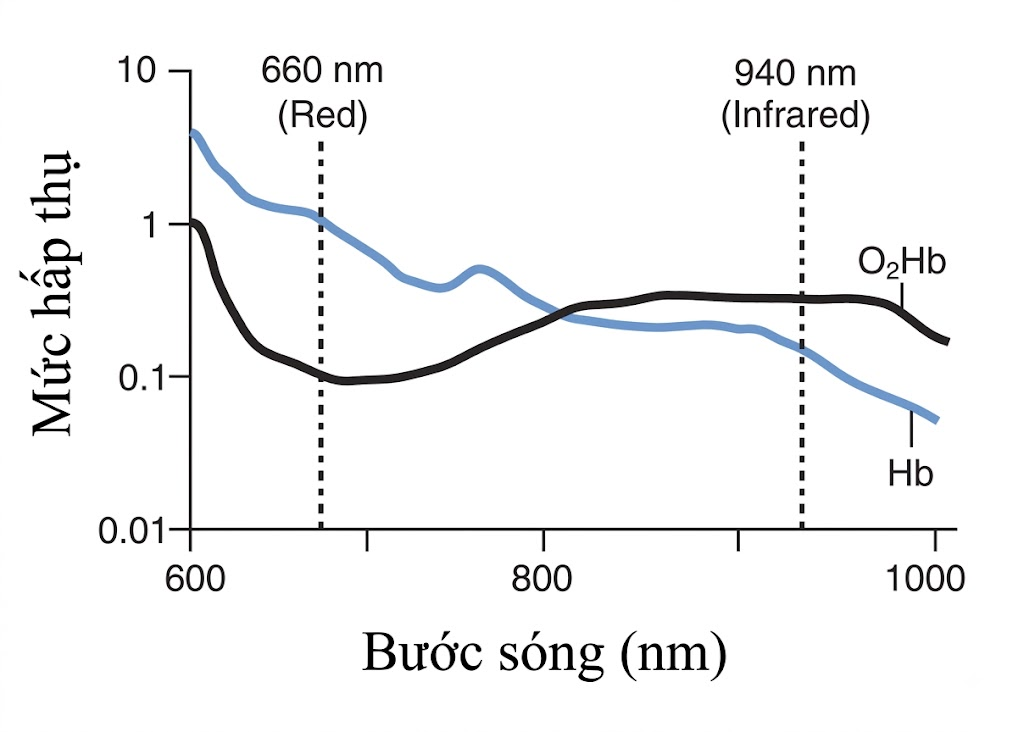
\includegraphics[width=0.6\textwidth]{image/cd16_image2.png}
\end{center}
\figcaption{2}{Mức hấp thụ ánh sáng của hai loại hemoglobin theo bước sóng.}

\vspace{6pt}

\tablecaption{1}{Mức hấp thụ tương đối của HbO\textsubscript{2} và Hb tại một số bước sóng.}

\renewcommand{\arraystretch}{1.4}
{\small
\setstretch{1.0}%
\begin{tabular}{|>{\raggedright\arraybackslash}m{0.34\textwidth}|>{\centering\arraybackslash}m{0.20\textwidth}|>{\centering\arraybackslash}m{0.20\textwidth}|}
\hline
\rowcolor{primaryBlue!12}
\textbf{Bước sóng} & \textbf{HbO\textsubscript{2}} & \textbf{Hb} \\
\hline
660 nm (ánh sáng đỏ) & 0,1 & 0,8 \\
\hline
800 nm (hồng ngoại gần) & 0,45 & 0,45 \\
\hline
940 nm (hồng ngoại) & 0,55 & 0,35 \\
\hline
\end{tabular}
}

\vspace{6pt}

[3] Cơ sở định lượng là \textbf{định luật Beer--Lambert}: lượng ánh sáng bị hấp thụ khi đi qua một lớp dung dịch tỷ lệ thuận với nồng độ chất hấp thụ và độ dày của lớp dung dịch. Vì vậy dung dịch càng đậm đặc hoặc lớp càng dày thì càng hấp thụ nhiều ánh sáng, và cường độ ánh sáng còn lại tới cảm biến càng nhỏ (Hình 3). Cảm biến thu nhận ánh sáng truyền qua mạch máu ở đầu ngón tay và chuyển thành tín hiệu điện để bộ xử lý phân tích. Các thành phần chính của máy được mô tả ở Hình 4.

\begin{center}
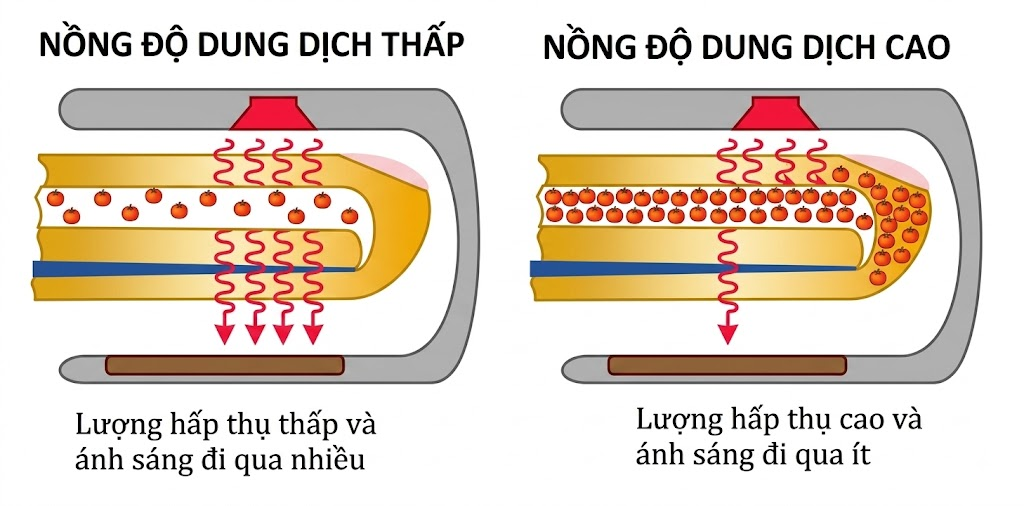
\includegraphics[width=0.5\textwidth]{image/cd16_image3.png}
\end{center}
\figcaption{3}{Khả năng hấp thụ ánh sáng của dung dịch ở các nồng độ khác nhau.}

\vspace{6pt}

\begin{center}
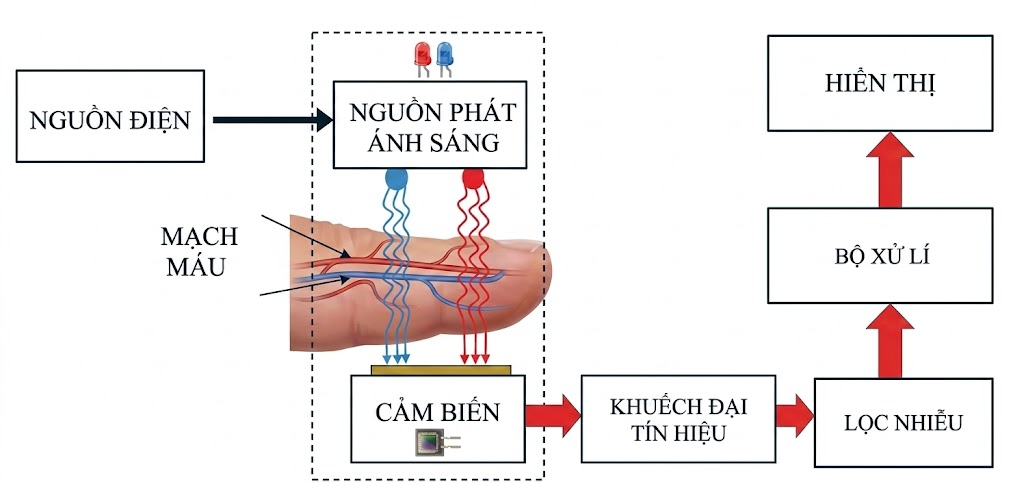
\includegraphics[width=0.65\textwidth]{image/cd16_image4.png}
\end{center}
\figcaption{4}{Cấu tạo các thành phần và cơ chế hoạt động chung của Pulse oximeter.}

\vspace{6pt}

[4] \textbf{Cơ chế xử lý tín hiệu.} Ở mao mạch và tĩnh mạch, lưu lượng máu chảy khá ổn định nên mật độ các thành phần máu gần như không đổi. Do đó cường độ ánh sáng mà cảm biến thu được từ hai loại mạch này gần như không đổi theo thời gian, gọi là \textbf{tín hiệu DC} (tín hiệu ổn định). Thành phần DC còn bao gồm phần ánh sáng đi qua động mạch ở thời điểm tim giãn. Ở động mạch, mỗi khi tim co, lượng máu dồn về nhiều hơn làm lớp máu dày lên nên hấp thụ thêm ánh sáng, khiến cường độ tới cảm biến giảm xuống. Phần chênh lệch tuần hoàn theo nhịp tim này gọi là \textbf{tín hiệu AC} (tín hiệu biến thiên):

\vspace{2pt}
\begin{center}
$\text{AC} = \text{(tín hiệu DC)} - \text{(tín hiệu ở thời điểm tim co)}$
\end{center}
\vspace{2pt}

[5] Dựa vào chu kỳ lặp lại của tín hiệu AC, bộ xử lý xác định thời gian một chu kỳ tim và suy ra nhịp tim. Sau khi khuếch đại và khử nhiễu, bộ xử lý tính tỷ số $R$ từ AC và DC của cả hai bước sóng theo công thức:

\vspace{2pt}
\begin{center}
$R = \dfrac{AC_{660} / DC_{660}}{AC_{940} / DC_{940}}$
\end{center}
\vspace{2pt}

[6] Từ tỷ số $R$, một hàm hiệu chuẩn $f(R)$ được lập trình sẵn sẽ cho ra giá trị SpO\textsubscript{2}. Trong giới hạn bài này, $f(R)$ được đơn giản hóa thành:

\vspace{2pt}
\begin{center}
$\text{SpO}_2 = 104 - 25 \times R$
\end{center}
\vspace{2pt}

(Ghi chú: trong thực tế, hàm $f(R)$ phức tạp hơn nhiều do nhiều yếu tố chi phối; công thức trên chỉ nhằm minh họa cơ chế.)

[7] Pulse oximeter có nhiều ưu điểm: tiện dụng, dễ sử dụng, không cần thủ thuật xâm lấn, theo dõi liên tục, cho kết quả nhanh, chi phí thấp. Bên cạnh đó máy có một số hạn chế: kết quả có thể sai lệch do ánh sáng môi trường, chuyển động của cơ thể, màu da, sơn móng tay hoặc hemoglobin bất thường. Ngoài ra máy còn có độ trễ 30--60 giây, chỉ chính xác trong khoảng SpO\textsubscript{2} từ 70\% đến 100\%, độ chính xác giảm mạnh khi SpO\textsubscript{2} dưới 70\%, và kém hiệu quả khi mạch đập yếu.

\vspace{6pt}

\hfill\textbf{Nguồn: Thầy Đào Anh Phúc biên soạn}

\end{readingpassage}
\vspace{2pt}

% === Câu 1: Trắc nghiệm ===
\question[Trắc nghiệm]{SpO\textsubscript{2} là chỉ số đo lường điều gì?}
\par\vspace{4pt}
\noindent\hangindent=2.2em\hangafter=1\choiceitem{A}{Tỷ lệ phần trăm hemoglobin trong máu động mạch có mang oxygen so với tổng lượng hemoglobin.}\par\vspace{4pt}
\noindent\hangindent=2.2em\hangafter=1\choiceitem{B}{Tỷ lệ oxygen hòa tan trong máu động mạch so với tổng lượng oxygen trong tĩnh mạch.}\par\vspace{4pt}
\noindent\hangindent=2.2em\hangafter=1\choiceitem{C}{Tỷ lệ phần trăm hemoglobin trong động mạch không mang oxygen so với tổng lượng hemoglobin.}\par\vspace{4pt}
\noindent\hangindent=2.2em\hangafter=1\choiceitem{D}{Tỷ lệ phần trăm oxygen được giải phóng từ hemoglobin mang oxygen trong động mạch.}\par\vspace{4pt}

% === Câu 2: Trắc nghiệm ===
\question[Trắc nghiệm]{Pulse oximeter hoạt động dựa trên nguyên lý nào?}
\par\vspace{4pt}
\noindent\hangindent=2.2em\hangafter=1\choiceitem{A}{Đo điện trở của da khi có dòng điện nhỏ đi qua.}\par\vspace{4pt}
\noindent\hangindent=2.2em\hangafter=1\choiceitem{B}{Đo mức hấp thụ ánh sáng của hemoglobin ở hai bước sóng.}\par\vspace{4pt}
\noindent\hangindent=2.2em\hangafter=1\choiceitem{C}{Đo nhiệt độ của máu truyền qua da đầu ngón tay.}\par\vspace{4pt}
\noindent\hangindent=2.2em\hangafter=1\choiceitem{D}{Phân tích sóng âm siêu thanh phản xạ từ mạch máu.}\par\vspace{4pt}

% === Câu 3: Trắc nghiệm ===
\question[Trắc nghiệm]{Oxyhemoglobin (HbO\textsubscript{2}) hấp thụ mạnh ánh sáng ở bước sóng nào?}
\par\vspace{4pt}
\noindent\choiceitem{A}{480 nm.}\hfill\choiceitem{B}{580 nm.}\hfill\choiceitem{C}{940 nm.}\hfill\choiceitem{D}{660 nm.}

% === Câu 4: Đúng/Sai ===
\question[Đúng/Sai]{Dựa vào toàn bài, hãy chọn Đúng hoặc Sai cho mỗi phát biểu về đặc điểm của pulse oximeter:}

\truefalsehead
\truefalseitem{Thiết bị sử dụng ba bước sóng ánh sáng khác nhau.}
\truefalseitem{Deoxyhemoglobin (Hb) hấp thụ mạnh ánh sáng đỏ 660 nm.}
\truefalseitem{Độ chính xác của máy giảm mạnh khi SpO\textsubscript{2} dưới 70\%.}
\truefalseitem{Thiết bị có độ trễ khoảng 30 đến 60 giây.}
\truefalseitem{Máy chỉ chính xác trong khoảng SpO\textsubscript{2} từ 60\% đến 100\%.}
\truefalseend

% === Câu 5: Trắc nghiệm ===
\question[Trắc nghiệm]{Theo định luật Beer--Lambert được nêu trong bài, khi nồng độ chất hấp thụ trong dung dịch tăng lên thì:}
\par\vspace{4pt}
\noindent\hangindent=2.2em\hangafter=1\choiceitem{A}{Lượng ánh sáng bị hấp thụ giảm đi.}\par\vspace{4pt}
\noindent\hangindent=2.2em\hangafter=1\choiceitem{B}{Việc hấp thụ ánh sáng không thay đổi.}\par\vspace{4pt}
\noindent\hangindent=2.2em\hangafter=1\choiceitem{C}{Lượng ánh sáng bị hấp thụ tăng lên.}\par\vspace{4pt}
\noindent\hangindent=2.2em\hangafter=1\choiceitem{D}{Dung dịch phản xạ lại toàn bộ ánh sáng.}\par\vspace{4pt}

% === Câu 6: Trắc nghiệm ===
\question[Trắc nghiệm]{Tín hiệu DC trong pulse oximeter có đặc điểm gì?}
\par\vspace{4pt}
\noindent\hangindent=2.2em\hangafter=1\choiceitem{A}{Biến thiên mạnh theo từng nhịp đập của tim.}\par\vspace{4pt}
\noindent\hangindent=2.2em\hangafter=1\choiceitem{B}{Chỉ xuất hiện đúng vào thời điểm tim co bóp.}\par\vspace{4pt}
\noindent\hangindent=2.2em\hangafter=1\choiceitem{C}{Khá ổn định do lưu lượng máu tương đối ổn định.}\par\vspace{4pt}
\noindent\hangindent=2.2em\hangafter=1\choiceitem{D}{Chỉ tồn tại ở bước sóng hồng ngoại 940 nm.}\par\vspace{4pt}

% === Câu 7: Trắc nghiệm ===
\question[Trắc nghiệm]{Công thức tính tín hiệu AC (tín hiệu biến thiên) là gì?}
\par\vspace{4pt}
\noindent\hangindent=2.2em\hangafter=1\choiceitem{A}{AC = Tín hiệu DC $-$ Tín hiệu ở thời điểm tim co.}\par\vspace{4pt}
\noindent\hangindent=2.2em\hangafter=1\choiceitem{B}{AC = Tín hiệu ở thời điểm tim co $-$ Tín hiệu DC.}\par\vspace{4pt}
\noindent\hangindent=2.2em\hangafter=1\choiceitem{C}{AC = Tín hiệu DC $\times$ Tín hiệu ở thời điểm tim co.}\par\vspace{4pt}
\noindent\hangindent=2.2em\hangafter=1\choiceitem{D}{AC = Tín hiệu DC $\div$ Tín hiệu ở thời điểm tim co.}\par\vspace{4pt}

% === Câu 8: Ghép đôi ===
\question[Ghép đôi]{Dựa vào Hình 4, ghép mỗi thành phần của pulse oximeter với chức năng tương ứng.}

\vspace{6pt}
\setstretch{1.3}

\textit{Cột B:}
\vspace{-6pt}
\par\vspace{4pt}
\noindent\hangindent=2.2em\hangafter=1\choiceitem{A}{Xử lý và tính toán dữ liệu.}\par\vspace{4pt}
\noindent\hangindent=2.2em\hangafter=1\choiceitem{B}{Phát ra hai bước sóng ánh sáng.}\par\vspace{4pt}
\noindent\hangindent=2.2em\hangafter=1\choiceitem{C}{Thu nhận ánh sáng và chuyển thành tín hiệu điện.}\par\vspace{4pt}
\noindent\hangindent=2.2em\hangafter=1\choiceitem{D}{Hiển thị kết quả SpO\textsubscript{2} và nhịp tim.}\par\vspace{4pt}

\vspace{6pt}

\renewcommand{\arraystretch}{1.6}
{\small\setstretch{1.0}
\begin{longtable}{|>{\raggedright\arraybackslash}m{0.55\textwidth}|>{\centering\arraybackslash}m{0.28\textwidth}|}
\hline
\rowcolor{primaryBlue!12}
\multicolumn{1}{|c|}{\cellcolor{primaryBlue!12}\textbf{Cột A}} & \cellcolor{primaryBlue!12}\textbf{Cột B} \\
\hline
\endfirsthead
\hline
\rowcolor{primaryBlue!12}
\multicolumn{1}{|c|}{\cellcolor{primaryBlue!12}\textbf{Cột A}} & \cellcolor{primaryBlue!12}\textbf{Cột B} \\
\hline
\endhead
1. Nguồn phát ánh sáng. & \dropbox[2.5cm] \\
\hline
2. Cảm biến. & \dropbox[2.5cm] \\
\hline
3. Bộ xử lý. & \dropbox[2.5cm] \\
\hline
4. Màn hình hiển thị. & \dropbox[2.5cm] \\
\hline
\end{longtable}
}

% === Câu 9: Ghép đôi ===
\question[Ghép đôi]{Ghép mỗi loại tín hiệu/đại lượng với đặc điểm tương ứng theo bài đọc.}

\vspace{6pt}
\setstretch{1.3}

\textit{Cột B:}
\vspace{-6pt}
\par\vspace{4pt}
\noindent\hangindent=2.2em\hangafter=1\choiceitem{A}{Biến thiên theo nhịp tim.}\par\vspace{4pt}
\noindent\hangindent=2.2em\hangafter=1\choiceitem{B}{Ổn định, gần như không đổi theo thời gian.}\par\vspace{4pt}
\noindent\hangindent=2.2em\hangafter=1\choiceitem{C}{Được tính từ AC và DC của cả hai bước sóng.}\par\vspace{4pt}
\noindent\hangindent=2.2em\hangafter=1\choiceitem{D}{Được suy ra từ hàm hiệu chuẩn $f(R)$.}\par\vspace{4pt}

\vspace{6pt}

\renewcommand{\arraystretch}{1.6}
{\small\setstretch{1.0}
\begin{longtable}{|>{\raggedright\arraybackslash}m{0.55\textwidth}|>{\centering\arraybackslash}m{0.28\textwidth}|}
\hline
\rowcolor{primaryBlue!12}
\multicolumn{1}{|c|}{\cellcolor{primaryBlue!12}\textbf{Cột A}} & \cellcolor{primaryBlue!12}\textbf{Cột B} \\
\hline
\endfirsthead
\hline
\rowcolor{primaryBlue!12}
\multicolumn{1}{|c|}{\cellcolor{primaryBlue!12}\textbf{Cột A}} & \cellcolor{primaryBlue!12}\textbf{Cột B} \\
\hline
\endhead
1. Tín hiệu DC. & \dropbox[2.5cm] \\
\hline
2. Tín hiệu AC. & \dropbox[2.5cm] \\
\hline
3. Tỷ số R. & \dropbox[2.5cm] \\
\hline
4. SpO\textsubscript{2}. & \dropbox[2.5cm] \\
\hline
\end{longtable}
}

% === Câu 10: Trắc nghiệm ===
\question[Trắc nghiệm]{Theo công thức trong bài, nếu $R = 0{,}4$ thì SpO\textsubscript{2} bằng bao nhiêu?}
\par\vspace{4pt}
\noindent\choiceitem{A}{92\%.}\hfill\choiceitem{B}{94\%.}\hfill\choiceitem{C}{96\%.}\hfill\choiceitem{D}{98\%.}

% === Câu 11: Chọn nhiều đáp án ===
\question[Chọn nhiều đáp án]{Những yếu tố nào sau đây có thể làm sai lệch kết quả đo của pulse oximeter?}
\par\vspace{4pt}
\noindent\hangindent=2.2em\hangafter=1\choiceitemBox{A}{Ánh sáng mạnh từ môi trường chiếu vào cảm biến.}\par\vspace{4pt}
\noindent\hangindent=2.2em\hangafter=1\choiceitemBox{B}{Bệnh nhân cử động tay trong khi đo.}\par\vspace{4pt}
\noindent\hangindent=2.2em\hangafter=1\choiceitemBox{C}{Sơn móng tay đậm màu ở ngón được đo.}\par\vspace{4pt}
\noindent\hangindent=2.2em\hangafter=1\choiceitemBox{D}{Đo trong phòng có nhiệt độ 25°C ổn định.}\par\vspace{4pt}
\noindent\hangindent=2.2em\hangafter=1\choiceitemBox{E}{Sự hiện diện của hemoglobin bất thường trong máu.}\par\vspace{4pt}
\noindent\hangindent=2.2em\hangafter=1\choiceitemBox{F}{Dùng máy để theo dõi liên tục trong nhiều giờ.}\par\vspace{4pt}

% === Câu 12: Điền khuyết ===
\question[Điền khuyết]{Một pulse oximeter ghi được: $AC_{660} = 0{,}64$; $DC_{660} = 10$; $AC_{940} = 2{,}0$; $DC_{940} = 10$. Dựa vào công thức trong bài:}

\vspace{4pt}
\begin{itemize}[leftmargin=2em, itemsep=4pt]
\item Tỷ số $R$ = \dropbox[2cm]
\item SpO\textsubscript{2} = \dropbox[2cm] \% (làm tròn đến số nguyên)
\end{itemize}

% === Câu 13: Đúng/Sai ===
\question[Đúng/Sai]{Dựa vào phần ``Cơ chế xử lý tín hiệu'', hãy chọn Đúng hoặc Sai cho mỗi phát biểu:}

\truefalsehead
\truefalseitem{Tín hiệu DC xuất hiện ở mọi loại mạch máu (động mạch, tĩnh mạch, mao mạch).}
\truefalseitem{Tín hiệu AC chủ yếu sinh ra từ máu ở động mạch đập theo nhịp tim.}
\truefalseitem{Khi tim co, lớp máu động mạch dày lên nên cường độ ánh sáng tới cảm biến giảm.}
\truefalseitem{Biên độ tín hiệu AC luôn lớn hơn biên độ tín hiệu DC ở cùng một bước sóng.}
\truefalseitem{Bộ xử lý suy ra nhịp tim từ độ lớn tuyệt đối của tín hiệu DC.}
\truefalseend

% === Câu 14: Trắc nghiệm ===
\question[Trắc nghiệm]{Vì sao pulse oximeter kém hiệu quả khi máu lưu thông ở mạch yếu?}
\par\vspace{4pt}
\noindent\hangindent=2.2em\hangafter=1\choiceitem{A}{Vì tín hiệu DC tăng vọt làm tràn bộ xử lý.}\par\vspace{4pt}
\noindent\hangindent=2.2em\hangafter=1\choiceitem{B}{Vì biên độ tín hiệu AC quá nhỏ, khó tách khỏi nhiễu.}\par\vspace{4pt}
\noindent\hangindent=2.2em\hangafter=1\choiceitem{C}{Vì tín hiệu AC trở nên quá lớn so với DC.}\par\vspace{4pt}
\noindent\hangindent=2.2em\hangafter=1\choiceitem{D}{Vì nguồn phát ánh sáng bị tắt khi mạch yếu.}\par\vspace{4pt}

% === Câu 15: Trắc nghiệm ===
\question[Trắc nghiệm]{Vì sao thiết bị bắt buộc dùng hai bước sóng thay vì chỉ một để xác định SpO\textsubscript{2}?}
\par\vspace{4pt}
\noindent\hangindent=2.2em\hangafter=1\choiceitem{A}{Vì một bước sóng dùng để đo nhịp tim, một bước sóng dùng để đo SpO\textsubscript{2} riêng biệt.}\par\vspace{4pt}
\noindent\hangindent=2.2em\hangafter=1\choiceitem{B}{Vì lập tỷ số $R$ giúp khử ảnh hưởng của độ dày mô và lưu lượng máu.}\par\vspace{4pt}
\noindent\hangindent=2.2em\hangafter=1\choiceitem{C}{Vì một bước sóng không đủ năng lượng để xuyên qua đầu ngón tay.}\par\vspace{4pt}
\noindent\hangindent=2.2em\hangafter=1\choiceitem{D}{Vì dùng hai bước sóng sẽ giúp máy hiển thị kết quả nhanh hơn hẳn.}\par\vspace{4pt}

% === Câu 16: Trắc nghiệm ===
\question[Trắc nghiệm]{Khi ngộ độc khí CO, máu sinh ra carboxyhemoglobin (COHb); ở bước sóng 660 nm, COHb hấp thụ ánh sáng gần giống oxyhemoglobin (HbO\textsubscript{2}). Vì pulse oximeter chỉ giả định trong máu có hai dạng Hb và HbO\textsubscript{2}, kết quả SpO\textsubscript{2} ở bệnh nhân ngộ độc CO nặng sẽ như thế nào?}
\par\vspace{4pt}
\noindent\hangindent=2.2em\hangafter=1\choiceitem{A}{Đọc thấp hơn thực tế vì COHb chặn toàn bộ ánh sáng đỏ.}\par\vspace{4pt}
\noindent\hangindent=2.2em\hangafter=1\choiceitem{B}{Đọc cao hơn thực tế vì máy tính COHb như HbO\textsubscript{2}.}\par\vspace{4pt}
\noindent\hangindent=2.2em\hangafter=1\choiceitem{C}{Máy báo lỗi và không cho ra kết quả nào.}\par\vspace{4pt}
\noindent\hangindent=2.2em\hangafter=1\choiceitem{D}{Không bị ảnh hưởng vì máy đã dùng tới hai bước sóng.}\par\vspace{4pt}

% === Câu 17: Trắc nghiệm ===
\question[Trắc nghiệm]{Dựa vào Bảng 1, tại bước sóng 660 nm, nhận định nào sau đây đúng?}
\par\vspace{4pt}
\noindent\hangindent=2.2em\hangafter=1\choiceitem{A}{Hb hấp thụ mạnh hơn HbO\textsubscript{2}, nên máu nghèo oxy hấp thụ ánh sáng đỏ nhiều hơn.}\par\vspace{4pt}
\noindent\hangindent=2.2em\hangafter=1\choiceitem{B}{HbO\textsubscript{2} hấp thụ mạnh hơn Hb, nên máu giàu oxy hấp thụ ánh sáng đỏ nhiều hơn.}\par\vspace{4pt}
\noindent\hangindent=2.2em\hangafter=1\choiceitem{C}{Hb và HbO\textsubscript{2} hấp thụ ánh sáng đỏ như nhau nên không phân biệt được.}\par\vspace{4pt}
\noindent\hangindent=2.2em\hangafter=1\choiceitem{D}{Cả hai dạng đều không hấp thụ ánh sáng đỏ ở bước sóng này.}\par\vspace{4pt}

% === Câu 18: Trắc nghiệm ===
\question[Trắc nghiệm]{Khi bệnh nhân cử động tay trong lúc đo, sai số xuất hiện chủ yếu do đâu?}
\par\vspace{4pt}
\noindent\hangindent=2.2em\hangafter=1\choiceitem{A}{Chuyển động làm tắt tạm thời nguồn phát ánh sáng của máy.}\par\vspace{4pt}
\noindent\hangindent=2.2em\hangafter=1\choiceitem{B}{Chuyển động tạo ra thành phần biến thiên giả cộng vào tín hiệu AC.}\par\vspace{4pt}
\noindent\hangindent=2.2em\hangafter=1\choiceitem{C}{Chuyển động làm tăng nhiệt độ ngón tay khiến máu loãng ra.}\par\vspace{4pt}
\noindent\hangindent=2.2em\hangafter=1\choiceitem{D}{Chuyển động làm thay đổi bước sóng ánh sáng do nguồn phát ra.}\par\vspace{4pt}

% === Câu 19: Đúng/Sai ===
\question[Đúng/Sai]{Dựa vào toàn bộ nội dung bài (kể cả Bảng 1 và các công thức), chọn Đúng hoặc Sai cho mỗi phát biểu:}

\truefalsehead
\truefalseitem{Mỗi dạng hemoglobin đều hấp thụ được cả hai bước sóng 660 nm và 940 nm, chỉ khác nhau về mức độ.}
\truefalseitem{AC và DC là hai nguồn sáng riêng biệt do máy phát ra.}
\truefalseitem{Theo Beer--Lambert, độ dày ngón tay là một yếu tố ảnh hưởng đến cường độ ánh sáng tới cảm biến.}
\truefalseitem{Theo công thức $\text{SpO}_2 = 104 - 25R$, $R$ càng lớn thì SpO\textsubscript{2} càng thấp, ứng với tỷ lệ deoxyhemoglobin càng cao.}
\truefalseitem{Vì $f(R)$ trong bài là hàm bậc nhất nên nó phản ánh chính xác mọi trường hợp lâm sàng.}
\truefalseend

% === Câu 20: Kéo thả ===
\question[Kéo thả]{Kéo các từ khóa cho sẵn vào chỗ trống phù hợp:}
\vspace{-4pt}
\dragitems{
\centering
    \dragitem{xâm lấn} \dragitem{Beer--Lambert} \dragitem{đỏ}\\[1pt]
    \dragitem{biến thiên} \dragitem{tỷ số R} \dragitem{hồng ngoại}\\[1pt]
    \dragitem{ổn định}
}

\setstretch{1.4}
Pulse oximeter là thiết bị không (1)\,\dropbox[2cm] dùng để đo SpO\textsubscript{2}, hoạt động dựa trên định luật (2)\,\dropbox[2cm]. Trong đó, deoxyhemoglobin hấp thụ mạnh ánh sáng (3)\,\dropbox[2cm] ở 660 nm. Thành phần tín hiệu (4)\,\dropbox[2cm] sinh ra do máu động mạch đập theo nhịp tim, còn thành phần DC gần như không đổi. Cuối cùng, bộ xử lý tính (5)\,\dropbox[2cm] từ AC và DC của cả hai bước sóng rồi suy ra SpO\textsubscript{2}.

% ============================================================


% ─────────────────────────────────────────────────────────────
% CHỦ ĐỀ 18: THUYẾT ĐỊA TÂM / NHẬT TÂM
% ─────────────────────────────────────────────────────────────
\newpage
\setcounter{qcounter}{0}

\phantomsection\label{b1_cd18}
\begin{topicbox}{\large CHỦ ĐỀ 18: THUYẾT ĐỊA TÂM / NHẬT TÂM}
\vspace{8pt}
\textit{Đọc đoạn văn sau và trả lời các câu hỏi.}
\end{topicbox}
\vspace{5pt}

\begin{readingpassage}
Trong lịch sử thiên văn học, có hai mô hình đối lập về cấu trúc hệ Mặt Trời: \textbf{thuyết địa tâm} và \textbf{thuyết nhật tâm}.

\textbf{Thuyết địa tâm} do Ptolemy (thế kỉ II sau CN) hệ thống hóa. Theo đó, Trái Đất nằm bất động ở trung tâm vũ trụ; Mặt Trăng, Mặt Trời, các hành tinh và các ngôi sao đều quay xung quanh Trái Đất theo những quỹ đạo tròn phức tạp gọi là \textit{ngoại luân} (epicycle). Mô hình này được Giáo hội Công giáo chấp nhận và thống trị suốt hơn 1400 năm.

\textbf{Thuyết nhật tâm} được Nicolaus Copernicus đề xuất vào thế kỉ XVI. Copernicus cho rằng Mặt Trời mới là trung tâm, các hành tinh -- bao gồm cả Trái Đất -- quay xung quanh Mặt Trời theo quỹ đạo tròn. Sau đó, Galileo Galilei dùng kính thiên văn quan sát thấy bốn mặt trăng quay quanh Sao Mộc, chứng tỏ không phải mọi thiên thể đều quay quanh Trái Đất, củng cố thuyết nhật tâm.

Johannes Kepler (1609--1619) hoàn thiện mô hình Copernicus bằng ba định luật:
\begin{itemize}[leftmargin=*, itemsep=2pt]
\item \textbf{Định luật I:} Quỹ đạo của mỗi hành tinh là một hình elip với Mặt Trời nằm tại một tiêu điểm.
\item \textbf{Định luật II:} Đường thẳng nối Mặt Trời với hành tinh quét diện tích bằng nhau trong những khoảng thời gian bằng nhau.
\item \textbf{Định luật III:} Bình phương chu kì quỹ đạo tỉ lệ với lập phương bán trục lớn: $T^2 \propto a^3$.
\end{itemize}

Isaac Newton sau đó giải thích cơ chế vật lí của các định luật Kepler thông qua lực hấp dẫn vạn vật. Bảng dưới đây tổng hợp số liệu quan sát của sáu hành tinh gần Mặt Trời nhất (tính theo đơn vị thiên văn AU và năm địa cầu yr):

\vspace{4pt}
\tablecaption{1}{Số liệu quỹ đạo của các hành tinh trong hệ Mặt Trời.}
\renewcommand{\arraystretch}{1.3}
\setstretch{1.0}%
\begin{longtable}{|l|c|c|c|c|c|}
\hline
\rowcolor{primaryBlue!10}
\textbf{Hành tinh} & $T$ (yr) & $a$ (AU) & $T^2$ & $a^3$ & $T^2/a^3$ \\
\hline
\endfirsthead
\hline
\rowcolor{primaryBlue!10}
\textbf{Hành tinh} & $T$ (yr) & $a$ (AU) & $T^2$ & $a^3$ & $T^2/a^3$ \\
\hline
\endhead
Sao Thủy & 0{,}241 & 0{,}387 & 0{,}058 & 0{,}058 & 1{,}00 \\
\hline
Sao Kim & 0{,}615 & 0{,}723 & 0{,}378 & 0{,}378 & 1{,}00 \\
\hline
Trái Đất & 1{,}000 & 1{,}000 & 1{,}000 & 1{,}000 & 1{,}00 \\
\hline
Sao Hỏa & 1{,}881 & 1{,}524 & 3{,}538 & 3{,}540 & 1{,}00 \\
\hline
Sao Mộc & 11{,}86 & 5{,}203 & 140{,}7 & 140{,}9 & 1{,}00 \\
\hline
Sao Thổ & 29{,}46 & 9{,}537 & 867{,}9 & 867{,}1 & 1{,}00 \\
\hline
\end{longtable}

\hfill\textbf{Nguồn: ACT -- American College Testing}
\end{readingpassage}

\question[Trắc nghiệm]{Thuyết địa tâm được hệ thống hóa bởi nhà khoa học nào?}
\par\vspace{4pt}
\noindent\choiceitem{A}{Copernicus}\hfill\choiceitem{B}{Galileo}\hfill\choiceitem{C}{Ptolemy}\hfill\choiceitem{D}{Kepler}

\question[Trắc nghiệm]{Theo thuyết địa tâm, thiên thể nằm ở trung tâm vũ trụ là?}
\par\vspace{4pt}
\noindent\choiceitem{A}{Mặt Trời}\hfill\choiceitem{B}{Trái Đất}\hfill\choiceitem{C}{Mặt Trăng}\hfill\choiceitem{D}{Sao Mộc}

\question[Trắc nghiệm]{Hành tinh X có chu kì quỹ đạo $T_X = 10\,\text{yr}$, hành tinh Y có chu kì $T_Y = 40\,\text{yr}$. Theo định luật III Kepler, tỉ số bán trục lớn $a_Y / a_X$ bằng?}
\par\vspace{4pt}
\noindent\choiceitem{A}{$2$}\hfill\choiceitem{B}{$\sqrt[3]{4}$}\hfill\choiceitem{C}{$4$}\hfill\choiceitem{D}{$2\sqrt[3]{2}$}

\question[Đúng/Sai]{Dựa vào thông tin trong bài đọc, đánh giá tính Đúng/Sai của các mệnh đề sau:}

\truefalsehead
\truefalseitem{Thuyết nhật tâm của Copernicus đã bác bỏ hoàn toàn thuyết địa tâm vì đặt Mặt Trời vào trung tâm thay cho Trái Đất.}
\truefalseitem{Thuyết địa tâm không giải thích được chuyển động nghịch hành (retrograde motion) của các hành tinh mà không cần dùng đến ngoại luân.}
\truefalseitem{Newton đã cung cấp cơ sở vật lí cho các định luật Kepler thông qua lực hấp dẫn vạn vật.}
\truefalseitem{Theo định luật III Kepler, bán trục lớn quỹ đạo tỉ lệ thuận với chu kì quỹ đạo của hành tinh.}
\truefalseend

\question[Trắc nghiệm]{Điểm khác biệt chính giữa mô hình nhật tâm của Copernicus và mô hình của Kepler là gì?}
\par\vspace{4pt}
\noindent\hangindent=2.2em\hangafter=1\choiceitem{A}{Vị trí của Mặt Trời}\par\vspace{4pt}
\noindent\hangindent=2.2em\hangafter=1\choiceitem{B}{Số lượng hành tinh được biết}\par\vspace{4pt}
\noindent\hangindent=2.2em\hangafter=1\choiceitem{C}{Hình dạng quỹ đạo hành tinh}\par\vspace{4pt}
\noindent\hangindent=2.2em\hangafter=1\choiceitem{D}{Tốc độ chuyển động của hành tinh}\par\vspace{4pt}

\question[Trắc nghiệm]{Hành tinh A có chu kì $T_A = 8\,\text{yr}$. Hành tinh B có bán trục lớn quỹ đạo gấp 2 lần hành tinh A. Chu kì $T_B$ của hành tinh B bằng bao nhiêu năm?}
\par\vspace{4pt}
\noindent\choiceitem{A}{$64\,\text{yr}$}\hfill\choiceitem{B}{$4\,\text{yr}$}\hfill\choiceitem{C}{$55{,}23\,\text{yr}$}\hfill\choiceitem{D}{$22{,}63\,\text{yr}$}

\question[Trắc nghiệm]{Galileo dùng bằng chứng nào để lập luận rằng không phải mọi thiên thể đều quay quanh Trái Đất?}
\par\vspace{4pt}
\noindent\hangindent=2.2em\hangafter=1\choiceitem{A}{Quan sát các pha của Sao Kim}\par\vspace{4pt}
\noindent\hangindent=2.2em\hangafter=1\choiceitem{B}{Quan sát bề mặt Mặt Trăng}\par\vspace{4pt}
\noindent\hangindent=2.2em\hangafter=1\choiceitem{C}{Phát hiện bốn mặt trăng quay quanh Sao Mộc}\par\vspace{4pt}
\noindent\hangindent=2.2em\hangafter=1\choiceitem{D}{Quan sát vết đen trên Mặt Trời}\par\vspace{4pt}

\question[Trắc nghiệm]{Điểm khác biệt cốt lõi giữa thuyết địa tâm và thuyết nhật tâm là gì?}
\par\vspace{4pt}
\noindent\hangindent=2.2em\hangafter=1\choiceitem{A}{Số lượng hành tinh trong hệ Mặt Trời}\par\vspace{4pt}
\noindent\hangindent=2.2em\hangafter=1\choiceitem{B}{Sự tồn tại của Mặt Trăng quay quanh Trái Đất}\par\vspace{4pt}
\noindent\hangindent=2.2em\hangafter=1\choiceitem{C}{Thiên thể nào nằm ở trung tâm: Trái Đất hay Mặt Trời}\par\vspace{4pt}
\noindent\hangindent=2.2em\hangafter=1\choiceitem{D}{Thuyết địa tâm sử dụng toán học còn thuyết nhật tâm thì không}\par\vspace{4pt}

\question[Kéo thả]{Bốn hành tinh giả định Alpha, Beta, Gamma, Delta có bán trục lớn quỹ đạo lần lượt là $a = 0{,}5\,\text{AU}$; $a = 4\,\text{AU}$; $a = 1{,}5\,\text{AU}$ và $a = 9\,\text{AU}$. Hãy sắp xếp các hành tinh theo thứ tự chu kì quỹ đạo tăng dần (từ ngắn nhất đến dài nhất).}
\vspace{-4pt}
\dragitems{%
\dragitem{Alpha}
\dragitem{Beta}
\dragitem{Gamma}
\dragitem{Delta}
}

\setstretch{1.4}
Thứ tự (chu kì tăng dần): \dropbox[2cm] $\rightarrow$ \dropbox[2cm] $\rightarrow$ \dropbox[2cm] $\rightarrow$ \dropbox[2cm]

\question[Trắc nghiệm]{Mô hình thuyết địa tâm cần dùng đến nhiều ngoại luân (epicycle) phức tạp, trong khi thuyết nhật tâm kết hợp định luật Kepler không cần dùng ngoại luân. Điều này hàm ý gì theo nguyên tắc khoa học?}
\par\vspace{4pt}
\noindent\hangindent=2.2em\hangafter=1\choiceitem{A}{Thuyết địa tâm chính xác hơn vì có nhiều tham số điều chỉnh hơn}\par\vspace{4pt}
\noindent\hangindent=2.2em\hangafter=1\choiceitem{B}{Cả hai mô hình đều đúng ngang nhau vì đều dự đoán được vị trí hành tinh}\par\vspace{4pt}
\noindent\hangindent=2.2em\hangafter=1\choiceitem{C}{Mô hình có ít giả định hơn được ưu tiên hơn nếu cho kết quả dự đoán tương đương}\par\vspace{4pt}
\noindent\hangindent=2.2em\hangafter=1\choiceitem{D}{Số lượng ngoại luân không liên quan đến giá trị khoa học của mô hình}\par\vspace{4pt}

% ─────────────────────────────────────────────────────────────
% CHỦ ĐỀ 19: LỰC HẤP DẪN
% ─────────────────────────────────────────────────────────────
\newpage
\setcounter{qcounter}{0}

\phantomsection\label{b1_cd19}
\begin{topicbox}{\large CHỦ ĐỀ 19: QUAN ĐIỂM VỀ LỰC HẤP DẪN}
\vspace{8pt}
\textit{Đọc đoạn văn sau và trả lời các câu hỏi.}
\end{topicbox}
\vspace{5pt}

\begin{readingpassage}
\textbf{Quan điểm của Isaac Newton}

Isaac Newton (1687) mô tả lực hấp dẫn là lực tác dụng từ xa giữa hai vật có khối lượng. Công thức định lượng:
$$F = G\frac{m_1 m_2}{r^2}$$
trong đó $G = 6{,}674 \times 10^{-11}\,\text{N·m}^2/\text{kg}^2$ là hằng số hấp dẫn, $m_1$, $m_2$ là khối lượng hai vật và $r$ là khoảng cách giữa chúng. Mô hình Newton giả định không-thời gian phẳng tuyệt đối và lực hấp dẫn truyền tức thời. Nó mô tả chính xác chuyển động của các hành tinh trong điều kiện thông thường và là nền tảng của cơ học thiên thể cổ điển.

Tuy nhiên, Newton không giải thích được \textit{cơ chế} truyền lực hấp dẫn, và mô hình của ông không dự đoán chính xác sự tiến động cận nhật (perihelion precession) của Sao Thủy -- sai lệch khoảng 43'' mỗi thế kỉ so với quan sát.

\textbf{Quan điểm của Albert Einstein}

Albert Einstein (1915) đề xuất \textit{thuyết tương đối rộng} (General Relativity) -- một mô hình hoàn toàn khác về bản chất hấp dẫn. Theo Einstein, hấp dẫn không phải là lực mà là biểu hiện của độ cong không-thời gian. Khối lượng và năng lượng làm cong không-thời gian, và các vật thể chuyển động theo \textit{đường trắc địa} (geodesic) -- đường thẳng nhất có thể trong không-thời gian cong đó.

Phương trình trường Einstein:
$$G_{\mu\nu} = \frac{8\pi G}{c^4} T_{\mu\nu}$$
trong đó $G_{\mu\nu}$ mô tả độ cong không-thời gian, $T_{\mu\nu}$ là tenxơ năng lượng-xung lượng. Thuyết tương đối rộng dự đoán chính xác sự tiến động cận nhật của Sao Thủy, sự uốn cong ánh sáng gần vật thể khối lượng lớn, và sự giãn nở thời gian trong trường hấp dẫn mạnh -- tất cả đều được xác nhận bởi thực nghiệm.

Trong điều kiện trường hấp dẫn yếu và vận tốc nhỏ so với tốc độ ánh sáng, hai mô hình cho kết quả gần như đồng nhất. Nhưng trong điều kiện cực đoan (lỗ đen, sóng hấp dẫn, GPS độ chính xác cao), chỉ mô hình Einstein mới cho kết quả đúng.

\hfill\textbf{Nguồn: ACT -- American College Testing}
\end{readingpassage}

\question[Trắc nghiệm]{Phát biểu nào sau đây là \textbf{đúng} về mối quan hệ giữa mô hình Newton và Einstein?}
\par\vspace{4pt}
\noindent\hangindent=2.2em\hangafter=1\choiceitem{A}{Mô hình Einstein hoàn toàn phủ nhận kết quả của mô hình Newton trong mọi trường hợp}\par\vspace{4pt}
\noindent\hangindent=2.2em\hangafter=1\choiceitem{B}{Hai mô hình cho kết quả giống hệt nhau trong điều kiện trường hấp dẫn mạnh}\par\vspace{4pt}
\noindent\hangindent=2.2em\hangafter=1\choiceitem{C}{Mô hình Newton luôn chính xác hơn vì đơn giản hơn}\par\vspace{4pt}
\noindent\hangindent=2.2em\hangafter=1\choiceitem{D}{Trong điều kiện thông thường, hai mô hình cho kết quả xấp xỉ nhau, nhưng trong điều kiện cực đoan chỉ mô hình Einstein mới đúng}\par\vspace{4pt}

\question[Trắc nghiệm]{Ai là người đề xuất thuyết tương đối rộng?}
\par\vspace{4pt}
\noindent\hangindent=2.2em\hangafter=1\choiceitem{A}{Isaac Newton}\par\vspace{4pt}
\noindent\hangindent=2.2em\hangafter=1\choiceitem{B}{Albert Einstein}\par\vspace{4pt}
\noindent\hangindent=2.2em\hangafter=1\choiceitem{C}{Johannes Kepler}\par\vspace{4pt}
\noindent\hangindent=2.2em\hangafter=1\choiceitem{D}{Galileo Galilei}\par\vspace{4pt}

\question[Trắc nghiệm]{Hai vật có khối lượng $m_1 = 10\,\text{kg}$ và $m_2 = 50\,\text{kg}$ cách nhau $r = 2\,\text{m}$. Lực hấp dẫn giữa chúng (lấy $G = 6{,}674 \times 10^{-11}\,\text{N·m}^2/\text{kg}^2$) là bao nhiêu?}
\par\vspace{4pt}
\noindent\hangindent=2.2em\hangafter=1\choiceitem{A}{$8{,}34 \times 10^{-9}\,\text{N}$}\par\vspace{4pt}
\noindent\hangindent=2.2em\hangafter=1\choiceitem{B}{$6{,}67 \times 10^{-9}\,\text{N}$}\par\vspace{4pt}
\noindent\hangindent=2.2em\hangafter=1\choiceitem{C}{$1{,}67 \times 10^{-8}\,\text{N}$}\par\vspace{4pt}
\noindent\hangindent=2.2em\hangafter=1\choiceitem{D}{$3{,}34 \times 10^{-9}\,\text{N}$}\par\vspace{4pt}

\question[Đúng/Sai]{Dựa vào thông tin trong bài đọc, đánh giá tính Đúng/Sai của các mệnh đề sau:}

\truefalsehead
\truefalseitem{Mô hình Newton giả định không-thời gian phẳng tuyệt đối và lực hấp dẫn truyền tức thời.}
\truefalseitem{Mô hình Newton không giải thích được chính xác sự tiến động cận nhật của Sao Thủy.}
\truefalseitem{Trong điều kiện trường hấp dẫn yếu, mô hình Newton là xấp xỉ tốt của mô hình Einstein.}
\truefalseitem{Theo Einstein, khối lượng và năng lượng làm cong không-thời gian, và các vật chuyển động theo đường trắc địa trong không-thời gian cong đó.}
\truefalseend

\question[Trắc nghiệm]{Công thức tính lực hấp dẫn của Newton là?}
\par\vspace{4pt}
\noindent\hangindent=2.2em\hangafter=1\choiceitem{A}{$F = G(m_1 + m_2)/r^2$}\par\vspace{4pt}
\noindent\hangindent=2.2em\hangafter=1\choiceitem{B}{$F = Gm_1m_2/r^3$}\par\vspace{4pt}
\noindent\hangindent=2.2em\hangafter=1\choiceitem{C}{$F = G\dfrac{m_1 m_2}{r^2}$}\par\vspace{4pt}
\noindent\hangindent=2.2em\hangafter=1\choiceitem{D}{$F = G\dfrac{m_1 m_2}{r}$}\par\vspace{4pt}

\question[Trắc nghiệm]{Hiện tượng nào sau đây được thuyết tương đối rộng của Einstein dự đoán mà mô hình Newton không dự đoán chính xác được?}
\par\vspace{4pt}
\noindent\hangindent=2.2em\hangafter=1\choiceitem{A}{Chuyển động elip của các hành tinh}\par\vspace{4pt}
\noindent\hangindent=2.2em\hangafter=1\choiceitem{B}{Lực hút giữa Trái Đất và Mặt Trăng}\par\vspace{4pt}
\noindent\hangindent=2.2em\hangafter=1\choiceitem{C}{Sự uốn cong của ánh sáng khi đi gần vật thể có khối lượng lớn}\par\vspace{4pt}
\noindent\hangindent=2.2em\hangafter=1\choiceitem{D}{Gia tốc rơi tự do trên bề mặt Trái Đất}\par\vspace{4pt}

\question[Trắc nghiệm]{Theo thuyết tương đối rộng của Einstein, các vật thể trong trường hấp dẫn chuyển động theo?}
\par\vspace{4pt}
\noindent\hangindent=2.2em\hangafter=1\choiceitem{A}{Đường thẳng trong không gian Euclid}\par\vspace{4pt}
\noindent\hangindent=2.2em\hangafter=1\choiceitem{B}{Đường trắc địa (geodesic) trong không-thời gian cong}\par\vspace{4pt}
\noindent\hangindent=2.2em\hangafter=1\choiceitem{C}{Đường tròn tuyệt đối quanh nguồn hấp dẫn}\par\vspace{4pt}
\noindent\hangindent=2.2em\hangafter=1\choiceitem{D}{Đường xoắn ốc hội tụ về phía nguồn hấp dẫn}\par\vspace{4pt}

\question[Trắc nghiệm]{Nếu khoảng cách giữa hai vật tăng gấp 3, lực hấp dẫn giữa chúng thay đổi như thế nào (theo mô hình Newton)?}
\par\vspace{4pt}
\noindent\hangindent=2.2em\hangafter=1\choiceitem{A}{Giảm đi 3 lần}\par\vspace{4pt}
\noindent\hangindent=2.2em\hangafter=1\choiceitem{B}{Tăng lên 9 lần}\par\vspace{4pt}
\noindent\hangindent=2.2em\hangafter=1\choiceitem{C}{Giảm đi 9 lần}\par\vspace{4pt}
\noindent\hangindent=2.2em\hangafter=1\choiceitem{D}{Giảm đi 6 lần}\par\vspace{4pt}

\question[Đúng/Sai]{Xét hai vật thể A và B tương tác hấp dẫn. Đánh giá tính Đúng/Sai của các mệnh đề sau:}

\truefalsehead
\truefalseitem{Nếu khoảng cách tăng gấp 2 và khối lượng $m_2$ tăng gấp 2, lực hấp dẫn giữa A và B sẽ giảm đi một nửa.}
\truefalseitem{Việc hai mô hình cho kết quả gần giống nhau trong điều kiện thông thường không có nghĩa là chúng mô tả cùng một cơ chế vật lí.}
\truefalseitem{Sự sai lệch 43''/thế kỉ trong tiến động cận nhật Sao Thủy là bằng chứng cho thấy cần một mô hình tốt hơn Newton cho trường hấp dẫn mạnh -- không phải vì Sao Thủy quá nặng mà vì nó quá gần Mặt Trời.}
\truefalseitem{Mô hình Newton vẫn đủ chính xác cho các tính toán ngắn hạn quỹ đạo Sao Thủy, nhưng sai số tích lũy theo thời gian.}
\truefalseend

\question[Kéo thả]{Điền vào chỗ trống để hoàn thành đoạn văn sau về sự kiểm chứng của hai mô hình hấp dẫn:}
\vspace{-4pt}
\dragitems{

\centering
    \dragitem{lệch dần} \dragitem{khớp chính xác} \dragitem{mạnh}\\[1pt]
    \dragitem{Einstein} \dragitem{lỗi tích lũy}

}

\setstretch{1.4}
Quan sát tinh vi cho thấy vị trí cận nhật của Sao Thủy (1)\,\dropbox[2.5cm] so với dự đoán Newton sau mỗi chu kì. Mô hình của (2)\,\dropbox[2.5cm] dự đoán (3)\,\dropbox[2.5cm] với giá trị quan sát. Điều này xảy ra vì trường hấp dẫn Mặt Trời tại vị trí Sao Thủy đủ (4)\,\dropbox[2.5cm] để gây ra hiệu ứng tương đối tính đáng kể. Sau nhiều thế kỉ, (5)\,\dropbox[2.5cm] theo Newton trở nên không thể bỏ qua.

% ─────────────────────────────────────────────────────────────
% CHỦ ĐỀ 20: MỰC NƯỚC THẤP VÙNG HỒ LỚN
% ─────────────────────────────────────────────────────────────
\newpage
\setcounter{qcounter}{0}

\phantomsection\label{b1_cd20}
\begin{topicbox}{\large CHỦ ĐỀ 20: MỰC NƯỚC THẤP VÙNG HỒ LỚN}
\vspace{8pt}
\textit{Đọc đoạn văn sau và trả lời các câu hỏi.}
\end{topicbox}
\vspace{5pt}

\begin{readingpassage}
Hệ thống Ngũ Hồ (Great Lakes) gồm năm hồ lớn -- Thượng, Michigan, Huron, Erie và Ontario -- tạo thành hệ thống nước ngọt bề mặt lớn nhất thế giới, chiếm khoảng 21\% tổng lượng nước ngọt bề mặt của Trái Đất. Từ giữa thập niên 1960, mực nước ở nhiều hồ đã giảm xuống mức thấp kỉ lục. Hai nhà khoa học đưa ra những lí giải trái chiều về nguyên nhân.

\textbf{Nhà khoa học 1 (nguyên nhân tự nhiên)}

Sự dao động mực nước ở Ngũ Hồ là hiện tượng tự nhiên đã xảy ra trong hàng nghìn năm, chịu chi phối bởi các yếu tố khí hậu. Lượng mưa và lượng bốc hơi -- hai thành phần chính của cân bằng nước trong hồ -- biến động theo chu kì nhiều thập niên do các kiểu thời tiết tự nhiên như El Niño và dao động thập niên Thái Bình Dương (PDO). Giai đoạn mực nước thấp hiện nay tương ứng với pha khô hạn của chu kì tự nhiên. Không có bằng chứng thuyết phục cho thấy hoạt động của con người là nguyên nhân chính; những biến động tương tự đã từng xảy ra trước khi có kênh đào hay nạo vét quy mô lớn.

\textbf{Nhà khoa học 2 (hoạt động con người)}

Mực nước giảm là hậu quả trực tiếp của nhiều can thiệp kĩ thuật do con người thực hiện. Việc nạo vét sâu các con sông St. Clair và Detroit -- nối hồ Huron với hồ Erie -- làm tăng tốc độ thoát nước ra khỏi hệ thống, hạ mực nước hồ Huron và Michigan vĩnh viễn. Ngoài ra, kênh đào Chicago đã chuyển nước từ hồ Michigan sang lưu vực sông Mississippi, làm mất đi một lượng nước đáng kể không được hoàn trả. Tổng hợp lại, các can thiệp này cộng hưởng để kéo mực nước xuống thấp hơn mức mà các yếu tố tự nhiên có thể tạo ra.

\hfill\textbf{Nguồn: ACT -- American College Testing}
\end{readingpassage}

\question[Trắc nghiệm]{Nhà khoa học 1 nhận định như thế nào về vai trò của biến đổi khí hậu toàn cầu?}
\par\vspace{4pt}
\noindent\hangindent=2.2em\hangafter=1\choiceitem{A}{Biến đổi khí hậu là nguyên nhân chính gây giảm mực nước}\par\vspace{4pt}
\noindent\hangindent=2.2em\hangafter=1\choiceitem{B}{Nhà khoa học 1 không đề cập đến biến đổi khí hậu mà chỉ quy kết cho dao động tự nhiên theo chu kì}\par\vspace{4pt}
\noindent\hangindent=2.2em\hangafter=1\choiceitem{C}{Biến đổi khí hậu làm tăng lượng bốc hơi, gây giảm mực nước}\par\vspace{4pt}
\noindent\hangindent=2.2em\hangafter=1\choiceitem{D}{Biến đổi khí hậu không liên quan đến hệ thống Ngũ Hồ}\par\vspace{4pt}

\question[Trắc nghiệm]{Theo bài đọc, kể từ khi nào mực nước Ngũ Hồ bắt đầu đạt mức thấp kỉ lục?}
\par\vspace{4pt}
\noindent\hangindent=2.2em\hangafter=1\choiceitem{A}{Đầu thập niên 1950}\par\vspace{4pt}
\noindent\hangindent=2.2em\hangafter=1\choiceitem{B}{Giữa thập niên 1960}\par\vspace{4pt}
\noindent\hangindent=2.2em\hangafter=1\choiceitem{C}{Đầu thập niên 1970}\par\vspace{4pt}
\noindent\hangindent=2.2em\hangafter=1\choiceitem{D}{Cuối thập niên 1980}\par\vspace{4pt}

\question[Đúng/Sai]{Dựa vào thông tin trong bài đọc, đánh giá tính Đúng/Sai của các mệnh đề sau:}

\truefalsehead
\truefalseitem{Hệ thống Ngũ Hồ là hệ thống nước ngọt bề mặt lớn nhất thế giới.}
\truefalseitem{Nhà khoa học 1 cho rằng dao động mực nước hồ là kết quả của các chu kì khí hậu tự nhiên như El Niño và PDO, không phải do hoạt động con người.}
\truefalseitem{Theo nhà khoa học 2, việc nạo vét sông St. Clair và Detroit đã làm tăng tốc độ thoát nước, hạ mực nước hồ Michigan và Huron vĩnh viễn.}
\truefalseitem{Mực nước thấp của các hồ chỉ gây ra bất tiện về giao thông đường thủy mà không ảnh hưởng đến hệ sinh thái.}
\truefalseitem{Kênh đào Chicago đã chuyển nước từ hồ Michigan sang lưu vực sông Mississippi theo quan điểm của nhà khoa học 2.}
\truefalseend

\question[Trắc nghiệm]{Theo nhà khoa học 2, hoạt động nào gây tác động lớn nhất đến mực nước hồ?}
\par\vspace{4pt}
\noindent\hangindent=2.2em\hangafter=1\choiceitem{A}{Xây dựng cảng thương mại ven hồ}\par\vspace{4pt}
\noindent\hangindent=2.2em\hangafter=1\choiceitem{B}{Khai thác cát lòng hồ}\par\vspace{4pt}
\noindent\hangindent=2.2em\hangafter=1\choiceitem{C}{Xây đập trên sông Detroit}\par\vspace{4pt}
\noindent\hangindent=2.2em\hangafter=1\choiceitem{D}{Nạo vét sâu sông St. Clair và Detroit kết hợp với chuyển nước qua kênh đào Chicago}\par\vspace{4pt}

\question[Trắc nghiệm]{Điều gì mà \textbf{cả hai} nhà khoa học đều có thể đồng ý?}
\par\vspace{4pt}
\noindent\hangindent=2.2em\hangafter=1\choiceitem{A}{Lượng nước mất đi cần được bổ sung theo cách nào đó để ổn định mực nước}\par\vspace{4pt}
\noindent\hangindent=2.2em\hangafter=1\choiceitem{B}{Con người không có bất kì ảnh hưởng nào đến mực nước hồ}\par\vspace{4pt}
\noindent\hangindent=2.2em\hangafter=1\choiceitem{C}{Nguyên nhân duy nhất là biến đổi khí hậu}\par\vspace{4pt}
\noindent\hangindent=2.2em\hangafter=1\choiceitem{D}{Mực nước hồ sẽ tự phục hồi mà không cần can thiệp}\par\vspace{4pt}

\question[Điền khuyết]{Điền vào chỗ trống để hoàn thành đoạn văn sau về tác động của biến đổi khí hậu đến hệ thống Ngũ Hồ:}
\vspace{-4pt}
\dragitems{%
\dragitem{tăng bốc hơi}
\dragitem{lượng mưa}
\dragitem{mực nước}
\dragitem{nhiệt độ}
}

\setstretch{1.4}
Sự ấm lên toàn cầu làm (1)\,\dropbox[2.5cm] trung bình của khu vực tăng lên, dẫn đến (2)\,\dropbox[2.5cm] từ bề mặt hồ. Đồng thời, các thay đổi trong chế độ khí hậu ảnh hưởng đến (3)\,\dropbox[2.5cm] hàng năm trong khu vực. Sự kết hợp của hai yếu tố này đều có thể làm (4)\,\dropbox[2.5cm] trong hồ thay đổi theo hướng giảm.

\question[Trắc nghiệm]{Theo nhà khoa học 2, nước từ hồ Michigan bị chuyển hướng sang lưu vực của con sông nào?}
\par\vspace{4pt}
\noindent\hangindent=2.2em\hangafter=1\choiceitem{A}{Sông St. Lawrence}\par\vspace{4pt}
\noindent\hangindent=2.2em\hangafter=1\choiceitem{B}{Sông Mississippi}\par\vspace{4pt}
\noindent\hangindent=2.2em\hangafter=1\choiceitem{C}{Sông Ohio}\par\vspace{4pt}
\noindent\hangindent=2.2em\hangafter=1\choiceitem{D}{Sông Hudson}\par\vspace{4pt}

\question[Trắc nghiệm]{Bằng chứng nào sau đây, nếu đúng, sẽ làm \textbf{suy yếu} lập luận của nhà khoa học 1?}
\par\vspace{4pt}
\noindent\hangindent=2.2em\hangafter=1\choiceitem{A}{Mực nước hồ dao động theo chu kì 20 năm trong suốt 200 năm qua}\par\vspace{4pt}
\noindent\hangindent=2.2em\hangafter=1\choiceitem{B}{Tỉ lệ lượng mưa trên lượng bốc hơi duy trì ổn định trong 50 năm qua, trong khi mực nước vẫn giảm liên tục}\par\vspace{4pt}
\noindent\hangindent=2.2em\hangafter=1\choiceitem{C}{Nhiều hồ ở vùng khác trên thế giới cũng giảm mực nước trong cùng giai đoạn}\par\vspace{4pt}
\noindent\hangindent=2.2em\hangafter=1\choiceitem{D}{Hoạt động nạo vét bắt đầu từ thế kỉ XIX, trước khi mực nước bắt đầu giảm mạnh}\par\vspace{4pt}

\question[Trắc nghiệm]{Điều gì có thể \textbf{không} đúng về hệ thống Ngũ Hồ dựa theo bài đọc?}
\par\vspace{4pt}
\noindent\hangindent=2.2em\hangafter=1\choiceitem{A}{Ngũ Hồ chứa khoảng 21\% tổng lượng nước ngọt bề mặt Trái Đất}\par\vspace{4pt}
\noindent\hangindent=2.2em\hangafter=1\choiceitem{B}{Nước từ các hồ chảy trực tiếp ra Đại Tây Dương mà không qua bất kì hệ thống kết nối nào khác}\par\vspace{4pt}
\noindent\hangindent=2.2em\hangafter=1\choiceitem{C}{Sông St. Clair và Detroit nối hồ Huron với hồ Erie}\par\vspace{4pt}
\noindent\hangindent=2.2em\hangafter=1\choiceitem{D}{Kênh đào Chicago kết nối hồ Michigan với lưu vực sông Mississippi}\par\vspace{4pt}

\question[Trắc nghiệm]{Giả sử có bằng chứng cho thấy mực nước hồ Superior không thay đổi đáng kể kể từ khi hệ thống Soo Locks được xây dựng, trong khi mực nước hồ Michigan và Huron liên tục giảm. Điều này ảnh hưởng thế nào đến lập luận của hai nhà khoa học?}
\par\vspace{4pt}
\noindent\hangindent=2.2em\hangafter=1\choiceitem{A}{Ủng hộ nhà khoa học 1, vì Superior ổn định chứng tỏ nguyên nhân tự nhiên}\par\vspace{4pt}
\noindent\hangindent=2.2em\hangafter=1\choiceitem{B}{Bác bỏ cả hai nhà khoa học}\par\vspace{4pt}
\noindent\hangindent=2.2em\hangafter=1\choiceitem{C}{Củng cố nhà khoa học 2, vì sự khác biệt giữa các hồ gợi ý nguyên nhân cục bộ (can thiệp kĩ thuật), không phải toàn khu vực (khí hậu)}\par\vspace{4pt}
\noindent\hangindent=2.2em\hangafter=1\choiceitem{D}{Không ảnh hưởng đến lập luận của cả hai nhà khoa học}\par\vspace{4pt}


\newpage
% ╔════════════════════════════════════════════════════════════╗
% ║  B.II.2 — LUYỆN THEO CHUYÊN ĐỀ                          ║
% ╚════════════════════════════════════════════════════════════╝

% ── REDEFINITION cho B.II.2 ──
% B2 dùng label A/B/C/D inline trong text (khác B1 auto-label a/b/c)
\renewcommand{\truefalsehead}{%
    \par\vspace{6pt}%
    \begingroup
    \setstretch{1.0}%
    \small
    \renewcommand{\arraystretch}{1.8}%
    \begin{longtable}{|>{\raggedright\arraybackslash}m{0.72\textwidth}|>{\centering\arraybackslash}m{0.08\textwidth}|>{\centering\arraybackslash}m{0.08\textwidth}|}
    \hline
    \rowcolor{primaryBlue!12}
    \textbf{Nội dung} & \textbf{Đúng} & \textbf{Sai} \\
    \hline
    \endfirsthead
    \hline
    \rowcolor{primaryBlue!12}
    \textbf{Nội dung} & \textbf{Đúng} & \textbf{Sai} \\
    \hline
    \endhead
}

\renewcommand{\truefalseitem}[1]{%
    #1 & \tfcircle & \tfcircle \\
    \hline
}


\begin{center}
\begin{tikzpicture}
    \node[fill=sectionMid, rounded corners=8pt,
          inner sep=12pt, drop shadow={shadow xshift=2pt, shadow yshift=-2pt}] {
        \begin{minipage}{0.85\textwidth}
            \centering
\phantomsection\label{sec_bii2}
            {\color{white}\fontsize{24}{30}\selectfont\textbf{B.II.2. LUYỆN THEO CHUYÊN ĐỀ}}
        \end{minipage}
    };
\end{tikzpicture}
\end{center}
\vspace{12pt}

% === 3 chuyên đề B.II.2 (thứ tự: Protein Cry → Phospholipid → Phanh ABS) ===
\begin{center}
\begin{tikzpicture}
    \node[fill=primaryBlue, rounded corners=10pt,
          inner xsep=25pt, inner ysep=14pt,
          drop shadow={shadow xshift=2pt, shadow yshift=-2pt, opacity=0.3}]
    {%
        \color{white}\fontsize{22}{28}\selectfont\bfseries
\phantomsection\label{b2_chuyende1}
        Chuyên đề 1: Protein Cry%
    };
\end{tikzpicture}
\end{center}

\vspace{-8pt}

% ─────────────────────────────────────────────────────────────
% CHỦ ĐỀ 1: VI KHUẨN Bacillus thuringiensis (Bt)
% ─────────────────────────────────────────────────────────────
\setcounter{qcounter}{0}

\phantomsection\label{b2_cd1_1}
\begin{topicbox}{\large CHỦ ĐỀ 1: VI KHUẨN BACILLUS THURINGIENSIS (Bt) -- VŨ KHÍ SINH HỌC TRONG PHÒNG TRỪ SÂU}
\vspace{8pt}
\textit{Đọc đoạn văn sau và trả lời các câu hỏi.}
\vspace{6pt}
\end{topicbox}

\begin{readingpassage}[]

\setstretch{1.3}
Bacillus thuringiensis (Bt) là một loài vi khuẩn Gram dương, có khả năng sinh bào tử, phân bố rộng rãi trong tự nhiên, đặc biệt là trong đất. Được phát hiện lần đầu vào năm 1901 bởi nhà khoa học Nhật Bản Shigetane Ishiwata, vi khuẩn Bt đã trở thành một trong những tác nhân kiểm soát sinh học quan trọng nhất trong nông nghiệp hiện đại. Đặc biệt, Bt có khả năng sản xuất các protein độc tố đặc hiệu khác nhau có thể tiêu diệt ấu trùng nhiều loài côn trùng gây hại thuộc bộ Cánh vẩy (Lepidoptera), bộ Cánh cứng (Coleoptera), và bộ Hai cánh (Diptera), trong khi vẫn an toàn đối với con người.

Khi điều kiện môi trường thuận lợi, vi khuẩn Bt tích cực phân chia, sinh trưởng và gần như không tích lũy độc tố. Tuy nhiên, khi môi trường trở nên khắc nghiệt với nguồn dinh dưỡng cạn kiệt, vi khuẩn Bt bắt đầu quá trình tạo bào tử, tạo lớp ``áo giáp'' vững chắc và đưa quá trình trao đổi chất về mức tối thiểu.

\vspace{2pt}
\begin{center}
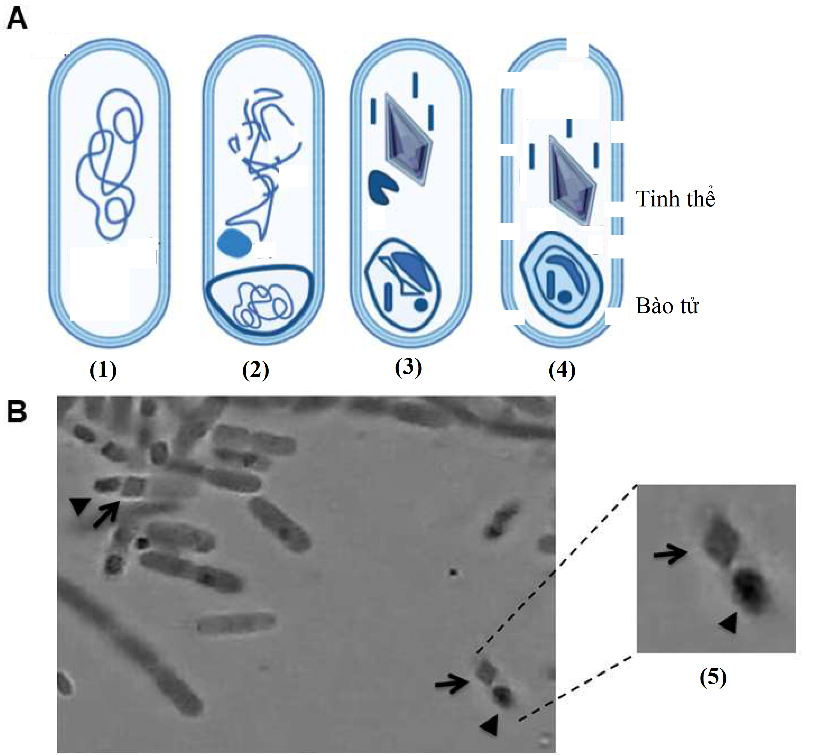
\includegraphics[width=0.50\textwidth]{image/cd_cry01_image1.png}
\end{center}
\figcaption{1}{(A) Quá trình hình thành bào tử và protein độc tố (Cry); (B) Hình chụp bào tử và độc tố. (1) Vi khuẩn ở trạng thái bình thường; (2)(3) Bắt đầu hình thành bào tử và tổng hợp protein độc tố; (4) Tế bào mẹ bị ly giải, giải phóng bào tử và tinh thể protein độc tố ra môi trường; (5) Ảnh chụp một bào tử đi kèm tinh thể protein độc tố.}

Trong quá trình tạo bào tử, vi khuẩn Bt đồng thời sản xuất các protein độc tố đặc biệt (Hình 1). Các protein này kết tinh thành cấu trúc gọi là tinh thể Cry (Crystal proteins). Khi quá trình hoàn tất, tế bào mẹ bị ly giải, giải phóng đồng thời bào tử và tinh thể protein ra ngoài. Bào tử giúp vi khuẩn tồn tại qua điều kiện bất lợi, khi gặp điều kiện thuận lợi, lớp ``áo giáp'' được phân giải, vi khuẩn trở về trạng thái hoạt động.

Khi ấu trùng sâu ăn phải lá cây có chứa bào tử và tinh thể Cry của Bt, quá trình diệt sâu bắt đầu với những bước sau (Hình 2):

\begin{enumerate}[leftmargin=2em, itemsep=3pt, topsep=2pt]
\item \textbf{Hòa tan tinh thể:} Môi trường kiềm mạnh (pH 9--12) trong ruột giữa của ấu trùng sâu tạo điều kiện lý tưởng để hòa tan tinh thể Cry thành các protein riêng lẻ chưa có tính độc -- tiền độc tố (protoxin).
\item \textbf{Kích hoạt độc tố:} Sau khi hòa tan, protein tiền độc tố (protoxin) được enzym protease trong ruột sâu cắt thành dạng độc tố hoạt động.
\item \textbf{Gắn kết với thụ thể:} Từng loại độc tố Cry ở trạng thái hoạt động chỉ gắn kết đặc hiệu với thụ thể của nó trên bề mặt tế bào biểu mô ruột của ấu trùng.
\item \textbf{Tạo lỗ thủng:} Sau khi gắn kết, độc tố kích hoạt hình thành các lỗ thủng (pore) trên màng tế bào, phá hủy niêm mạc ruột, phá vỡ cân bằng ion, rối loạn áp suất thẩm thấu, tràn dịch xoang cơ thể vào khoang ruột. Đồng thời bào tử ``cởi giáp'' thành vi khuẩn hoạt động, xâm nhập vào bên trong khoang ruột của sâu gây nhiễm trùng.
\item \textbf{Tê liệt và chết:} Sâu ngừng ăn, bị tê liệt và chết do sự phá hủy hệ tiêu hóa. Đồng thời, môi trường ruột sâu bị phá hủy tạo điều kiện cho bào tử Bt được kích hoạt loại bỏ ``áo giáp'', sử dụng chính ấu trùng làm nguồn dinh dưỡng để sinh trưởng và sinh sản nên thế hệ vi khuẩn mới.
\end{enumerate}

\vspace{2pt}
\begin{center}
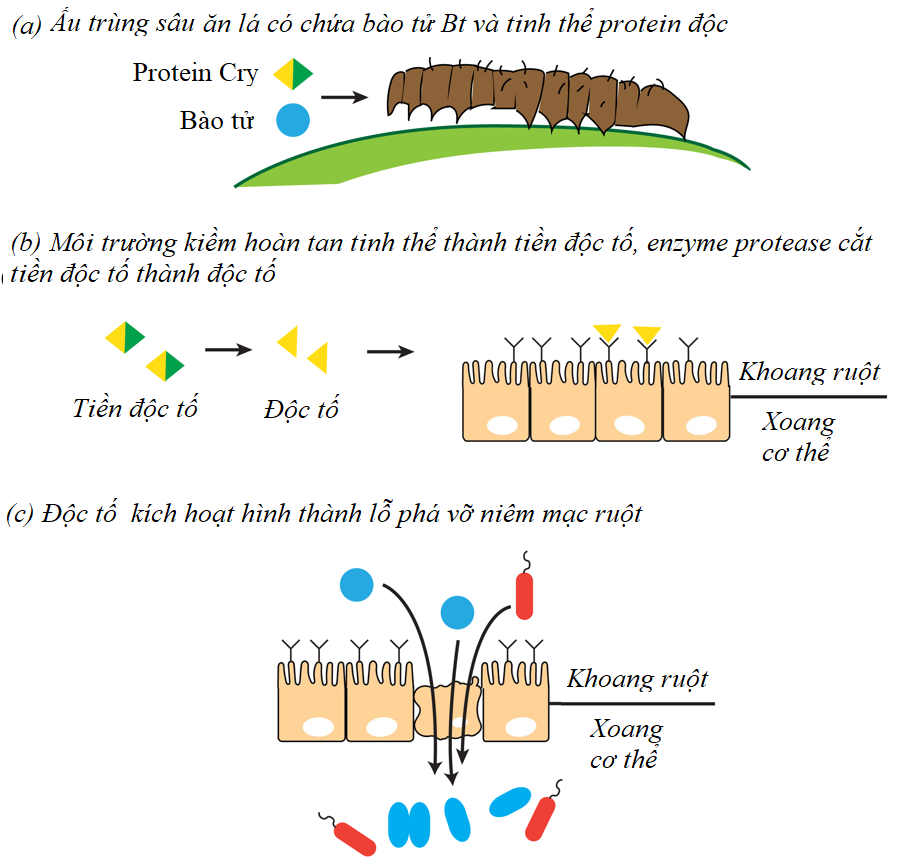
\includegraphics[width=0.65\textwidth]{image/cd_cry01_image2.png}
\end{center}
\figcaption{2}{Cơ chế gây độc của protein Cry lên ấu trùng sâu hại.}

Một điều đặc biệt là Bt không gây độc cho người và động vật có xương sống vì dạ dày người có pH axit (khoảng 1,5--3,5), không thích hợp để hòa tan và kích hoạt tinh thể Cry, khác với môi trường kiềm trong ruột sâu. Về mặt cơ chế, độc tố Cry chỉ có thể gắn kết với thụ thể đặc hiệu trên tế bào ruột của côn trùng mục tiêu nhưng tế bào ruột của người và động vật có xương sống không có các thụ thể này. Do đó, protein Cry sẽ bị phân giải bởi enzyme tiêu hóa giống như các loại protein khác. Đồng thời, các sản phẩm chứa Bt đã trải qua hàng chục năm thử nghiệm nghiêm ngặt và được chứng minh là an toàn cho người, động vật có xương sống khác và môi trường.

Chính nhờ tính an toàn và hiệu quả cao này, Bt đã trở thành một công cụ quan trọng trong nông nghiệp bền vững và sản xuất thực phẩm an toàn, góp phần giảm thiểu việc sử dụng hóa chất độc hại trong phòng trừ sâu bệnh. Con người có thể tạo bào tử vi khuẩn để phun lên cây trồng hoặc phân lập gene tạo protein Cry chuyển cho cây trồng tạo ra giống biến đổi gene có khả năng kháng sâu.

\hfill\textbf{Nguồn: Thầy Đào Anh Phúc biên soạn}
\end{readingpassage}
\vspace{2pt}
% ── CÂU HỎI CĐ 1 ──

% === Câu 1: Trắc nghiệm ===
\question[Trắc nghiệm]{Vi khuẩn Bacillus thuringiensis được phát hiện lần đầu tiên vào năm nào và bởi ai?}
\par\vspace{4pt}
\noindent\hangindent=2.2em\hangafter=1\choiceitem{A}{Năm 1901 bởi nhà khoa học Nhật Bản Shigetane Ishiwata.}\par\vspace{4pt}
\noindent\hangindent=2.2em\hangafter=1\choiceitem{B}{Năm 1910 bởi nhà khoa học Pháp Louis Pasteur.}\par\vspace{4pt}
\noindent\hangindent=2.2em\hangafter=1\choiceitem{C}{Năm 1901 bởi nhà khoa học Đức Ernst Berliner.}\par\vspace{4pt}
\noindent\hangindent=2.2em\hangafter=1\choiceitem{D}{Năm 1915 bởi nhà khoa học Nga Ilya Mechnikov.}\par\vspace{4pt}

% === Câu 2: Trắc nghiệm ===
\question[Trắc nghiệm]{Điều gì xảy ra khi môi trường trở nên khắc nghiệt với nguồn dinh dưỡng cạn kiệt đối với vi khuẩn Bt?}
\par\vspace{4pt}
\noindent\hangindent=2.2em\hangafter=1\choiceitem{A}{Vi khuẩn Bt ngừng sinh trưởng và chết hoàn toàn.}\par\vspace{4pt}
\noindent\hangindent=2.2em\hangafter=1\choiceitem{B}{Vi khuẩn Bt tiến hành quá trình hình thành bào tử.}\par\vspace{4pt}
\noindent\hangindent=2.2em\hangafter=1\choiceitem{C}{Vi khuẩn Bt phân chia nhanh hơn để tăng số lượng cá thể.}\par\vspace{4pt}
\noindent\hangindent=2.2em\hangafter=1\choiceitem{D}{Vi khuẩn Bt tự phân hủy để giải phóng các chất dinh dưỡng.}\par\vspace{4pt}

% === Câu 3: Chọn nhiều đáp án ===
\question[Chọn nhiều đáp án]{Các nhóm côn trùng nào sau đây bị ảnh hưởng bởi độc tố của vi khuẩn Bt?}
\par\vspace{4pt}
\noindent\hangindent=2.2em\hangafter=1\choiceitemBox{A}{Bộ Cánh vẩy (Lepidoptera).}\par\vspace{4pt}
\noindent\hangindent=2.2em\hangafter=1\choiceitemBox{B}{Bộ Cánh thẳng (Orthoptera).}\par\vspace{4pt}
\noindent\hangindent=2.2em\hangafter=1\choiceitemBox{C}{Bộ Cánh cứng (Coleoptera).}\par\vspace{4pt}
\noindent\hangindent=2.2em\hangafter=1\choiceitemBox{D}{Bộ Hai cánh (Diptera).}\par\vspace{4pt}
\noindent\hangindent=2.2em\hangafter=1\choiceitemBox{E}{Bộ Cánh nửa (Hemiptera).}\par\vspace{4pt}
\noindent\hangindent=2.2em\hangafter=1\choiceitemBox{F}{Bộ Cánh màng (Hymenoptera).}\par\vspace{4pt}

% === Câu 4: Chọn nhiều đáp án ===
\question[Chọn nhiều đáp án]{Những yếu tố nào khiến vi khuẩn Bt trở thành một công cụ quan trọng trong nông nghiệp bền vững?}
\par\vspace{4pt}
\noindent\hangindent=2.2em\hangafter=1\choiceitemBox{A}{An toàn cho người và động vật có xương sống.}\par\vspace{4pt}
\noindent\hangindent=2.2em\hangafter=1\choiceitemBox{B}{Hiệu quả cao trong phòng trừ sâu bệnh.}\par\vspace{4pt}
\noindent\hangindent=2.2em\hangafter=1\choiceitemBox{C}{Giảm thiểu việc sử dụng hóa chất độc hại.}\par\vspace{4pt}
\noindent\hangindent=2.2em\hangafter=1\choiceitemBox{D}{Dễ dàng phân hủy trong môi trường.}\par\vspace{4pt}
\noindent\hangindent=2.2em\hangafter=1\choiceitemBox{E}{Chi phí sản xuất thấp hơn thuốc trừ sâu hóa học.}\par\vspace{4pt}
\noindent\hangindent=2.2em\hangafter=1\choiceitemBox{F}{Có thể được sử dụng để tạo cây trồng biến đổi gene.}\par\vspace{4pt}

% === Câu 5: Trắc nghiệm ===
\question[Trắc nghiệm]{Trình tự nào dưới đây mô tả đúng quá trình diệt sâu của vi khuẩn Bt?}
\par\vspace{4pt}
\noindent\hangindent=2.2em\hangafter=1\choiceitem{A}{Ấu trùng ăn bào tử $\rightarrow$ Tế bào ruột bị phá hủy $\rightarrow$ Tinh thể Cry hòa tan $\rightarrow$ Tiền độc tố được kích hoạt $\rightarrow$ Sâu chết.}\par\vspace{4pt}
\noindent\hangindent=2.2em\hangafter=1\choiceitem{B}{Ấu trùng ăn bào tử $\rightarrow$ Tinh thể Cry hòa tan $\rightarrow$ Tiền độc tố được kích hoạt $\rightarrow$ Độc tố gắn kết với thụ thể $\rightarrow$ Tạo lỗ thủng $\rightarrow$ Tế bào ruột bị phá hủy $\rightarrow$ Sâu chết.}\par\vspace{4pt}
\noindent\hangindent=2.2em\hangafter=1\choiceitem{C}{Tinh thể Cry hòa tan $\rightarrow$ Bào tử xâm nhập vào ruột sâu $\rightarrow$ Độc tố gắn kết với thụ thể $\rightarrow$ Tạo lỗ thủng $\rightarrow$ Sâu chết.}\par\vspace{4pt}
\noindent\hangindent=2.2em\hangafter=1\choiceitem{D}{Bào tử xâm nhập vào ruột sâu $\rightarrow$ Tinh thể Cry hòa tan $\rightarrow$ Độc tố gắn kết với thụ thể $\rightarrow$ Sâu bị nhiễm trùng $\rightarrow$ Sâu chết.}\par\vspace{4pt}

% === Câu 6: Chọn nhiều đáp án ===
\question[Chọn nhiều đáp án]{Những đặc điểm nào dưới đây là đúng khi nói về protein Cry của vi khuẩn Bt?}
\par\vspace{4pt}
\noindent\hangindent=2.2em\hangafter=1\choiceitemBox{A}{Được tạo ra trong quá trình tạo bào tử.}\par\vspace{4pt}
\noindent\hangindent=2.2em\hangafter=1\choiceitemBox{B}{Ở dạng tinh thể khi giải phóng.}\par\vspace{4pt}
\noindent\hangindent=2.2em\hangafter=1\choiceitemBox{C}{Có tính độc ngay khi được tạo ra.}\par\vspace{4pt}
\noindent\hangindent=2.2em\hangafter=1\choiceitemBox{D}{Được hòa tan trong môi trường kiềm.}\par\vspace{4pt}
\noindent\hangindent=2.2em\hangafter=1\choiceitemBox{E}{Cần enzyme protease để kích hoạt.}\par\vspace{4pt}
\noindent\hangindent=2.2em\hangafter=1\choiceitemBox{F}{Tạo lỗ thủng trên màng tế bào ruột sâu.}\par\vspace{4pt}

% === Câu 7: Ghép đôi ===
\question[Ghép đôi]{Ghép đôi giữa trạng thái của vi khuẩn Bt với điều kiện môi trường tương ứng.}

\vspace{6pt}
\setstretch{1.3}

\textit{Cột B:}
\vspace{-6pt}
\par\vspace{4pt}
\noindent\hangindent=2.2em\hangafter=1\choiceitem{A}{Trong ruột sâu sau khi được ăn vào}\par\vspace{4pt}
\noindent\hangindent=2.2em\hangafter=1\choiceitem{B}{Điều kiện thuận lợi với đủ dinh dưỡng}\par\vspace{4pt}
\noindent\hangindent=2.2em\hangafter=1\choiceitem{C}{Tế bào mẹ bị ly giải}\par\vspace{4pt}
\noindent\hangindent=2.2em\hangafter=1\choiceitem{D}{Môi trường khắc nghiệt, dinh dưỡng cạn kiệt}\par\vspace{4pt}
\noindent\hangindent=2.2em\hangafter=1\choiceitem{E}{Sau khi sâu đã bị tê liệt và chết}\par\vspace{4pt}

\vspace{6pt}

\renewcommand{\arraystretch}{1.6}
{\small\setstretch{1.0}
\begin{longtable}{|>{\raggedright\arraybackslash}m{0.55\textwidth}|>{\centering\arraybackslash}m{0.28\textwidth}|}
\hline
\rowcolor{primaryBlue!12}
\multicolumn{1}{|c|}{\cellcolor{primaryBlue!12}\textbf{Cột A}} & \cellcolor{primaryBlue!12}\textbf{Cột B} \\
\hline
\endfirsthead
\hline
\rowcolor{primaryBlue!12}
\multicolumn{1}{|c|}{\cellcolor{primaryBlue!12}\textbf{Cột A}} & \cellcolor{primaryBlue!12}\textbf{Cột B} \\
\hline
\endhead
1. Tích cực phân chia, sinh trưởng & \dropbox[2.5cm] \\
\hline
2. Tạo bào tử và tổng hợp protein độc tố & \dropbox[2.5cm] \\
\hline
3. Bào tử và tinh thể độc tố được giải phóng & \dropbox[2.5cm] \\
\hline
4. Bào tử ``cởi giáp'' thành vi khuẩn hoạt động & \dropbox[2.5cm] \\
\hline
5. Vi khuẩn sử dụng ấu trùng làm nguồn dinh dưỡng & \dropbox[2.5cm] \\
\hline
\end{longtable}
}

% === Câu 8: Ghép đôi ===
\question[Ghép đôi]{Ghép đôi giữa các bước trong cơ chế diệt sâu với hiện tượng tương ứng.}

\vspace{6pt}
\setstretch{1.3}

\textit{Cột B:}
\vspace{-6pt}
\par\vspace{4pt}
\noindent\hangindent=2.2em\hangafter=1\choiceitem{A}{Sâu ngừng ăn, bị tê liệt và chết}\par\vspace{4pt}
\noindent\hangindent=2.2em\hangafter=1\choiceitem{B}{Tràn dịch xoang cơ thể vào khoang ruột}\par\vspace{4pt}
\noindent\hangindent=2.2em\hangafter=1\choiceitem{C}{Độc tố hoạt động gắn kết với thụ thể trên màng tế bào}\par\vspace{4pt}
\noindent\hangindent=2.2em\hangafter=1\choiceitem{D}{Môi trường kiềm mạnh hòa tan tinh thể Cry}\par\vspace{4pt}
\noindent\hangindent=2.2em\hangafter=1\choiceitem{E}{Enzyme protease cắt tiền độc tố thành dạng hoạt động}\par\vspace{4pt}

\vspace{6pt}

\renewcommand{\arraystretch}{1.6}
{\small\setstretch{1.0}
\begin{longtable}{|>{\raggedright\arraybackslash}m{0.55\textwidth}|>{\centering\arraybackslash}m{0.28\textwidth}|}
\hline
\rowcolor{primaryBlue!12}
\multicolumn{1}{|c|}{\cellcolor{primaryBlue!12}\textbf{Cột A}} & \cellcolor{primaryBlue!12}\textbf{Cột B} \\
\hline
\endfirsthead
\hline
\rowcolor{primaryBlue!12}
\multicolumn{1}{|c|}{\cellcolor{primaryBlue!12}\textbf{Cột A}} & \cellcolor{primaryBlue!12}\textbf{Cột B} \\
\hline
\endhead
1. Hòa tan tinh thể & \dropbox[2.5cm] \\
\hline
2. Kích hoạt độc tố & \dropbox[2.5cm] \\
\hline
3. Gắn kết với thụ thể & \dropbox[2.5cm] \\
\hline
4. Tạo lỗ thủng & \dropbox[2.5cm] \\
\hline
5. Tê liệt và chết & \dropbox[2.5cm] \\
\hline
\end{longtable}
}

% === Câu 9: Chọn nhiều đáp án ===
\question[Chọn nhiều đáp án]{Cơ chế nào gây chết cho sâu khi protein Cry tấn công lên tế bào niêm mạc ruột?}
\par\vspace{4pt}
\noindent\hangindent=2.2em\hangafter=1\choiceitemBox{A}{Phá hủy niêm mạc ruột thông qua việc tạo lỗ thủng trên màng tế bào.}\par\vspace{4pt}
\noindent\hangindent=2.2em\hangafter=1\choiceitemBox{B}{Phá vỡ cân bằng ion và rối loạn áp suất thẩm thấu trong tế bào ruột.}\par\vspace{4pt}
\noindent\hangindent=2.2em\hangafter=1\choiceitemBox{C}{Tràn dịch xoang cơ thể vào khoang ruột.}\par\vspace{4pt}
\noindent\hangindent=2.2em\hangafter=1\choiceitemBox{D}{Bào tử ``cởi giáp'' thành vi khuẩn hoạt động, xâm nhập và gây nhiễm trùng.}\par\vspace{4pt}
\noindent\hangindent=2.2em\hangafter=1\choiceitemBox{E}{Sâu ngừng ăn và bị tê liệt do sự phá hủy hệ tiêu hóa.}\par\vspace{4pt}
\noindent\hangindent=2.2em\hangafter=1\choiceitemBox{F}{Protein Cry gây đông máu trong hệ tuần hoàn của sâu.}\par\vspace{4pt}
\noindent\hangindent=2.2em\hangafter=1\choiceitemBox{G}{Độc tố xâm nhập vào hệ thần kinh và gây tổn thương não sâu.}\par\vspace{4pt}
\noindent\hangindent=2.2em\hangafter=1\choiceitemBox{H}{Protein Cry ức chế quá trình tổng hợp protein trong tế bào sâu.}\par\vspace{4pt}

% === Câu 10: Đúng/Sai ===
\question[Đúng/Sai]{Dựa vào bài đọc, những phát biểu nào sau đây là đúng hay sai?}

\truefalsehead
\truefalseitem{A. Vi khuẩn Bt là loài vi khuẩn sống kí sinh bắt buộc trên ấu trùng sâu}
\truefalseitem{B. Protein Cry là vũ khí giúp bào tử chống lại sự tấn công của ấu trùng sâu}
\truefalseitem{C. Có nhiều loại protein Cry khác nhau và được mã hóa bởi gene có trong Bt}
\truefalseitem{D. Protein Cry là chất kích thích sinh trưởng của Bt}
\truefalseitem{E. Protein Cry trực tiếp cung cấp dinh dưỡng cho Bt}
\truefalseitem{F. Protein Cry tạo ra một lượng lớn khi vi khuẩn Bt sinh trưởng và sinh sản}
\truefalseend

% === Câu 11: Chọn nhiều đáp án ===
\question[Chọn nhiều đáp án]{Vì sao tinh thể protein Cry không gây độc cho người?}
\par\vspace{4pt}
\noindent\hangindent=2.2em\hangafter=1\choiceitemBox{A}{Dạ dày người có pH axit (khoảng 1,5--3,5), không thích hợp để hòa tan và kích hoạt tinh thể Cry.}\par\vspace{4pt}
\noindent\hangindent=2.2em\hangafter=1\choiceitemBox{B}{Tế bào ruột của người không có các thụ thể đặc hiệu mà độc tố Cry cần gắn kết.}\par\vspace{4pt}
\noindent\hangindent=2.2em\hangafter=1\choiceitemBox{C}{Protein Cry bị phân giải bởi các enzyme tiêu hóa giống như các loại protein thông thường khác.}\par\vspace{4pt}
\noindent\hangindent=2.2em\hangafter=1\choiceitemBox{D}{Bào tử Bt không thể nảy mầm trong nhiệt độ cơ thể người.}\par\vspace{4pt}

% === Câu 12: Chọn nhiều đáp án ===
\question[Chọn nhiều đáp án]{Tại sao protein tinh thể độc chỉ gây hại cho một số nhóm côn trùng?}
\par\vspace{4pt}
\noindent\hangindent=2.2em\hangafter=1\choiceitemBox{A}{Độc tố Cry chỉ có thể gắn kết với thụ thể đặc hiệu có trên tế bào ruột của một số loài côn trùng mục tiêu.}\par\vspace{4pt}
\noindent\hangindent=2.2em\hangafter=1\choiceitemBox{B}{Một số loài côn trùng có môi trường kiềm trong ruột giữa không đạt ngưỡng để hòa tan và kích hoạt tinh thể Cry.}\par\vspace{4pt}
\noindent\hangindent=2.2em\hangafter=1\choiceitemBox{C}{Vi khuẩn Bt sản sinh ra nhiều loại protein Cry khác nhau, mỗi loại chỉ độc với một nhóm côn trùng cụ thể.}\par\vspace{4pt}
\noindent\hangindent=2.2em\hangafter=1\choiceitemBox{D}{Các loài côn trùng không thuộc nhóm mục tiêu có thể thiếu enzyme protease cần thiết để cắt tiền độc tố thành dạng hoạt động.}\par\vspace{4pt}

% === Câu 13: Trắc nghiệm ===
\question[Trắc nghiệm]{Các loại protein Cry khác nhau có các bước gây độc là giống nhau nhưng có đặc điểm riêng đặc trưng cho từng loại. Dựa vào cơ chế chung, giai đoạn nào sau đây sẽ thể hiện rõ sự khác biệt (tính đặc hiệu) trong gây độc giữa các loại protein Cry?}
\par\vspace{4pt}
\noindent\hangindent=2.2em\hangafter=1\choiceitem{A}{Cơ chế hòa tan tinh thể khác nhau.}\par\vspace{4pt}
\noindent\hangindent=2.2em\hangafter=1\choiceitem{B}{Enzym kích hoạt độc tố khác nhau.}\par\vspace{4pt}
\noindent\hangindent=2.2em\hangafter=1\choiceitem{C}{Gắn kết với các thụ thể khác nhau.}\par\vspace{4pt}
\noindent\hangindent=2.2em\hangafter=1\choiceitem{D}{Tạo lỗ thủng trên các tế bào khác nhau.}\par\vspace{4pt}
\noindent\hangindent=2.2em\hangafter=1\choiceitem{E}{Cơ chế gây tê liệt và làm chết sâu khác nhau.}\par\vspace{4pt}

% === Câu 14: Trắc nghiệm ===
\question[Trắc nghiệm]{Điều gì xảy ra khi sâu ăn phải bào tử và tinh thể Cry của vi khuẩn Bt nhưng ruột sâu không có khả năng hòa tan tinh thể?}
\par\vspace{4pt}
\noindent\hangindent=2.2em\hangafter=1\choiceitem{A}{Sâu vẫn bị tê liệt và chết do bào tử phát triển thành vi khuẩn hoạt động trong ruột.}\par\vspace{4pt}
\noindent\hangindent=2.2em\hangafter=1\choiceitem{B}{Tinh thể Cry và bào tử đi qua hệ tiêu hóa của sâu mà không gây hại đáng kể.}\par\vspace{4pt}
\noindent\hangindent=2.2em\hangafter=1\choiceitem{C}{Tinh thể Cry tích lũy trong cơ thể sâu và gây độc chậm sau vài ngày.}\par\vspace{4pt}
\noindent\hangindent=2.2em\hangafter=1\choiceitem{D}{Bào tử vẫn hoạt động và tiêu diệt sâu mặc dù tinh thể Cry không được hòa tan.}\par\vspace{4pt}


% ─────────────────────────────────────────────────────────────
% CHỦ ĐỀ 2: VI KHUẨN Agrobacterium
% ─────────────────────────────────────────────────────────────
\newpage
\setcounter{qcounter}{0}

\phantomsection\label{b2_cd1_2}
\begin{topicbox}{\large CHỦ ĐỀ 2: VI KHUẨN AGROBACTERIUM -- KỸ SƯ DI TRUYỀN TINH VI CỦA TỰ NHIÊN}
\vspace{8pt}
\textit{Đọc đoạn văn sau và trả lời các câu hỏi.}
\vspace{6pt}
\end{topicbox}

\begin{readingpassage}[]

\setstretch{1.3}
Trong tự nhiên, mối quan hệ ký sinh -- vật chủ thể hiện sự đa dạng và phức tạp đáng kinh ngạc. Một trong những chiến lược tinh vi nhất của vật ký sinh là cơ chế ``thao túng vật chủ'' để tạo ra ``bể chứa dinh dưỡng'' (nutrient sink). Thay vì chỉ đơn thuần bám vào và hút chất dinh dưỡng một cách thụ động, vật ký sinh có thể chủ động can thiệp vào quá trình trao đổi chất của vật chủ. Chúng khiến vật chủ ưu tiên vận chuyển chất dinh dưỡng đến chính nơi vật ký sinh đang cư ngụ.

Vi khuẩn đất Agrobacterium tumefaciens là minh chứng điển hình cho cơ chế này. Khi xâm nhập vào cơ thể thực vật, vi khuẩn A. tumefaciens thực hiện một ``thủ thuật'' sinh học tinh vi: chuyển gene gây tăng sinh tế bào vào bộ gene của cây chủ. Kết quả là tế bào thực vật nhận được gene này sẽ phân chia nhanh chóng một cách bất thường, tạo thành khối u được gọi là ``ung thư thực vật'' hay bệnh u sùi -- chính là ``bể chứa dinh dưỡng'' lý tưởng mà vi khuẩn đã thiết kế.

Công cụ mang và chuyển gene của vi khuẩn A. tumefaciens là một plasmid có tên Ti-plasmid (Tumor-inducing plasmid) (Hình 1a). Plasmid này chứa hai vùng gene cực kỳ quan trọng cho quá trình gây bệnh:

Thứ nhất là vùng T-DNA chứa các gene mã hóa enzyme tổng hợp các chất như auxin, cytokinin (hormone sinh trưởng thực vật) và opine (một loại chất rất cần thiết cho sự sinh trưởng của vi khuẩn). Khi được chuyển vào tế bào cây, những hormone này được sản xuất không kiểm soát, phá vỡ chu trình tế bào bình thường và khiến chúng phân chia liên tục tạo thành khối u (Hình 1b).

Thứ hai là vùng chứa các gene virulence (vir genes) -- bộ máy phức tạp giúp nhận biết tế bào thực vật, tạo kênh chuyển gene và đưa T-DNA vào bộ gene của cây chủ.

\vspace{2pt}
\begin{center}
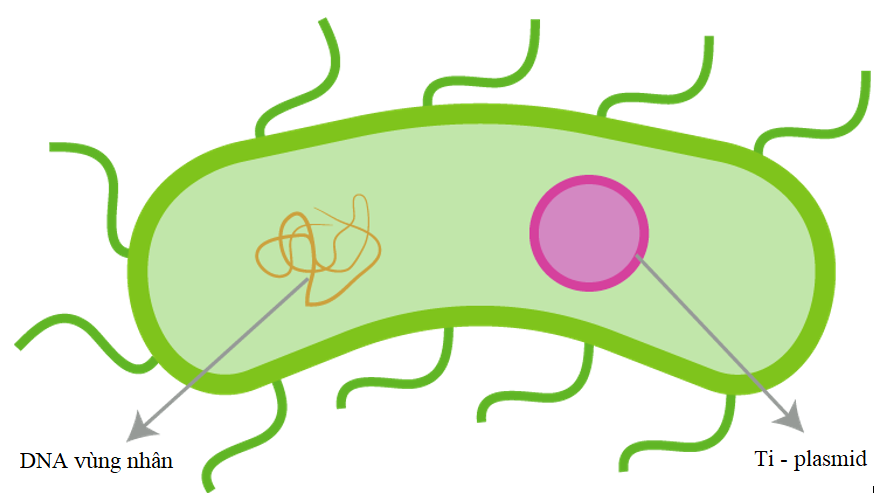
\includegraphics[width=0.45\textwidth]{image/cd_cry02_image1.png}
\hspace{0.5cm}
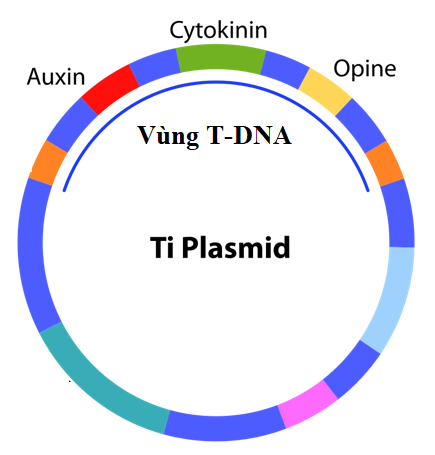
\includegraphics[width=0.35\textwidth]{image/cd_cry02_image2.png}
\end{center}
\figcaption{1}{(a) Vi khuẩn A. tumefaciens chứa Ti-plasmid; (b) Cấu trúc vùng T-DNA trên Ti-plasmid.}

Quá trình ``lây nhiễm'' của Agrobacterium là một ví dụ kinh điển về chuyển gene tự nhiên (Hình 2), diễn ra theo các bước sau:

\begin{enumerate}[leftmargin=2em, itemsep=3pt, topsep=2pt]
\item \textbf{Xâm nhập:} Khi thực vật có vết thương (do côn trùng cắn, hoặc tác động cơ học), các hợp chất phenolic do cây tiết ra sẽ hoạt động như tín hiệu hóa học, thu hút và kích hoạt vi khuẩn Agrobacterium.
\item \textbf{Kích hoạt và Chuyển giao:} Vi khuẩn bám vào thành tế bào thực vật. Các gen vir được kích hoạt, tạo ra một phức hợp protein có khả năng cắt lấy một sợi đơn của T-DNA và bao bọc nó. Phức hợp T-DNA này sau đó được bơm vào tế bào chất của thực vật thông qua một kênh vận chuyển đặc biệt.
\item \textbf{Tích hợp:} T-DNA di chuyển vào nhân tế bào và tích hợp một cách ngẫu nhiên vào bộ gen của cây chủ.
\item \textbf{Hình thành khối u:} Kể từ lúc này, tế bào thực vật đã được gắn gene của vi khuẩn. Các gene này sẽ tự động được kích hoạt sản xuất auxin, cytokinin và opine theo ``lập trình'' của T-DNA. Các hormone ``ép buộc'' cây gửi nhiều chất dinh dưỡng đến các tế bào phát triển thành khối u. Các tế bào khối u trở thành ``nô lệ'' giải phóng chất dinh dưỡng cho sự phát triển của quần thể vi khuẩn Agrobacterium.
\end{enumerate}

\vspace{2pt}
\begin{center}
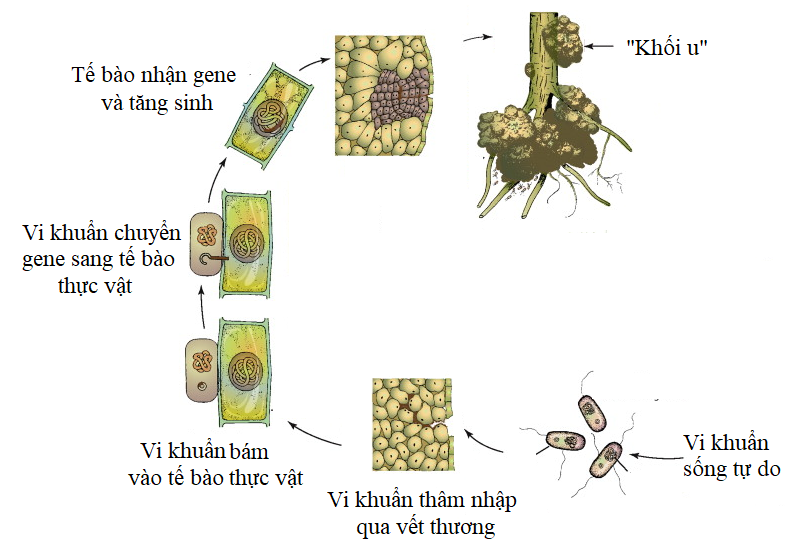
\includegraphics[width=0.7\textwidth]{image/cd_cry02_image3.png}
\end{center}
\figcaption{2}{Quá trình xâm nhập và chuyển gene của vi khuẩn Agrobacterium vào tế bào thực vật và hình thành khối u.}

Cơ chế này không chỉ là hiện tượng tự nhiên thú vị mà còn trở thành công cụ mạnh mẽ trong công nghệ sinh học hiện đại, giúp con người tạo ra cây trồng biến đổi gene. Trong công nghệ sinh học, các gene gây bệnh trong vùng T-DNA của Ti-plasmid được loại bỏ hoặc bất hoạt, sau đó gene cần chuyển được chèn vào vùng này, thường kèm theo gene đánh dấu chọn lọc.

\vspace{2pt}
\begin{center}
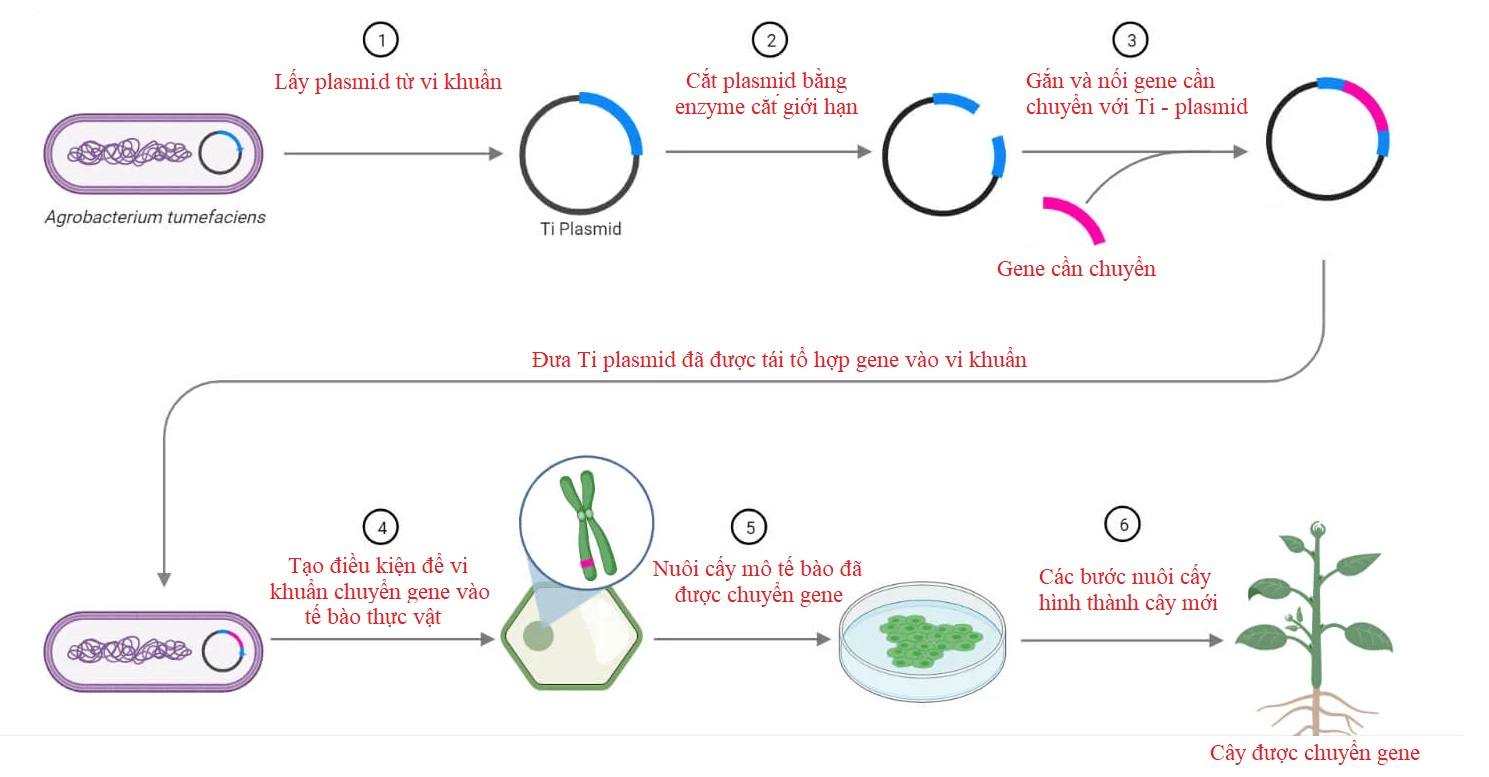
\includegraphics[width=0.75\textwidth]{image/cd_cry02_image4.png}
\end{center}
\figcaption{3}{Quy trình chuyển gene vào thực vật sử dụng Ti-plasmid của vi khuẩn Agrobacterium.}

\hfill\textbf{Nguồn: Thầy Đào Anh Phúc biên soạn}
\end{readingpassage}
\vspace{2pt}
% ── CÂU HỎI CĐ 2 ──

% === Câu 1: Trắc nghiệm ===
\question[Trắc nghiệm]{Theo bài đọc, cơ chế ``thao túng vật chủ'' của vi khuẩn Agrobacterium tumefaciens được thể hiện chủ yếu qua việc gì?}
\par\vspace{4pt}
\noindent\hangindent=2.2em\hangafter=1\choiceitem{A}{Vi khuẩn bám vào bề mặt lá và hút chất dinh dưỡng một cách thụ động.}\par\vspace{4pt}
\noindent\hangindent=2.2em\hangafter=1\choiceitem{B}{Vi khuẩn chuyển gene gây tăng sinh tế bào để tạo ``bể chứa dinh dưỡng''.}\par\vspace{4pt}
\noindent\hangindent=2.2em\hangafter=1\choiceitem{C}{Vi khuẩn tiết ra enzyme phá hủy thành tế bào để xâm nhập vào cây.}\par\vspace{4pt}
\noindent\hangindent=2.2em\hangafter=1\choiceitem{D}{Vi khuẩn sản xuất độc tố để làm suy yếu hệ miễn dịch của thực vật.}\par\vspace{4pt}

% === Câu 2: Chọn nhiều đáp án ===
\question[Chọn nhiều đáp án]{Dựa vào bài đọc, những thành phần nào sau đây có trong vùng T-DNA của Ti-plasmid?}
\par\vspace{4pt}
\noindent\hangindent=2.2em\hangafter=1\choiceitemBox{A}{Gene mã hóa enzyme tổng hợp auxin.}\par\vspace{4pt}
\noindent\hangindent=2.2em\hangafter=1\choiceitemBox{B}{Gene virulence (vir genes) giúp nhận biết tế bào thực vật.}\par\vspace{4pt}
\noindent\hangindent=2.2em\hangafter=1\choiceitemBox{C}{Gene mã hóa enzyme tổng hợp cytokinin.}\par\vspace{4pt}
\noindent\hangindent=2.2em\hangafter=1\choiceitemBox{D}{Gene tạo kênh chuyển T-DNA vào bộ gen của cây chủ.}\par\vspace{4pt}
\noindent\hangindent=2.2em\hangafter=1\choiceitemBox{E}{Gene mã hóa enzyme tổng hợp opine.}\par\vspace{4pt}
\noindent\hangindent=2.2em\hangafter=1\choiceitemBox{F}{Gene tạo phức hợp protein có khả năng cắt lấy một sợi đơn của T-DNA.}\par\vspace{4pt}

% === Câu 3: Trắc nghiệm ===
\question[Trắc nghiệm]{Khối u được tạo thành do hoạt động của vi khuẩn Agrobacterium được gọi là gì?}
\par\vspace{4pt}
\noindent\hangindent=2.2em\hangafter=1\choiceitem{A}{Khối u lành tính hoặc bướu cây.}\par\vspace{4pt}
\noindent\hangindent=2.2em\hangafter=1\choiceitem{B}{``Ung thư thực vật'' hay bệnh u sùi.}\par\vspace{4pt}
\noindent\hangindent=2.2em\hangafter=1\choiceitem{C}{Hạch lympho hoặc tuyến nước.}\par\vspace{4pt}
\noindent\hangindent=2.2em\hangafter=1\choiceitem{D}{Nốt sần hoặc mụn nhọt thực vật.}\par\vspace{4pt}

% === Câu 4: Trắc nghiệm ===
\question[Trắc nghiệm]{Ti-plasmid là viết tắt của thuật ngữ nào?}
\par\vspace{4pt}
\noindent\hangindent=2.2em\hangafter=1\choiceitem{A}{Tissue-inducing plasmid (plasmid tạo mô).}\par\vspace{4pt}
\noindent\hangindent=2.2em\hangafter=1\choiceitem{B}{Tumor-inducing plasmid (plasmid gây u).}\par\vspace{4pt}
\noindent\hangindent=2.2em\hangafter=1\choiceitem{C}{Transformation-inducing plasmid (plasmid gây biến đổi).}\par\vspace{4pt}
\noindent\hangindent=2.2em\hangafter=1\choiceitem{D}{Transfer-inducing plasmid (plasmid chuyển gene).}\par\vspace{4pt}

% === Câu 5: Trắc nghiệm ===
\question[Trắc nghiệm]{Opine được đề cập trong bài đọc là gì?}
\par\vspace{4pt}
\noindent\hangindent=2.2em\hangafter=1\choiceitem{A}{Một loại hormone sinh trưởng thực vật tương tự auxin.}\par\vspace{4pt}
\noindent\hangindent=2.2em\hangafter=1\choiceitem{B}{Một enzyme giúp phân giải thành tế bào thực vật.}\par\vspace{4pt}
\noindent\hangindent=2.2em\hangafter=1\choiceitem{C}{Một loại chất rất cần thiết cho sự sinh trưởng của vi khuẩn.}\par\vspace{4pt}
\noindent\hangindent=2.2em\hangafter=1\choiceitem{D}{Một protein vận chuyển giúp T-DNA di chuyển vào nhân tế bào.}\par\vspace{4pt}

% === Câu 6: Trắc nghiệm ===
\question[Trắc nghiệm]{Trong quá trình xâm nhập, yếu tố nào đóng vai trò như tín hiệu hóa học thu hút vi khuẩn?}
\par\vspace{4pt}
\noindent\hangindent=2.2em\hangafter=1\choiceitem{A}{Các hormone auxin và cytokinin do cây tiết ra.}\par\vspace{4pt}
\noindent\hangindent=2.2em\hangafter=1\choiceitem{B}{Các hợp chất phenolic do cây tiết ra tại vết thương.}\par\vspace{4pt}
\noindent\hangindent=2.2em\hangafter=1\choiceitem{C}{Các enzyme tiêu hóa do vi khuẩn sản xuất.}\par\vspace{4pt}
\noindent\hangindent=2.2em\hangafter=1\choiceitem{D}{Các protein miễn dịch do cây tạo ra để chống vi khuẩn.}\par\vspace{4pt}

% === Câu 7: Chọn nhiều đáp án ===
\question[Chọn nhiều đáp án]{Những chức năng nào thuộc về vùng vir genes?}
\par\vspace{4pt}
\noindent\hangindent=2.2em\hangafter=1\choiceitemBox{A}{Nhận biết tế bào thực vật.}\par\vspace{4pt}
\noindent\hangindent=2.2em\hangafter=1\choiceitemBox{B}{Sản xuất hormone auxin và cytokinin.}\par\vspace{4pt}
\noindent\hangindent=2.2em\hangafter=1\choiceitemBox{C}{Tạo kênh chuyển gene.}\par\vspace{4pt}
\noindent\hangindent=2.2em\hangafter=1\choiceitemBox{D}{Đưa T-DNA vào bộ gen của cây chủ.}\par\vspace{4pt}
\noindent\hangindent=2.2em\hangafter=1\choiceitemBox{E}{Tổng hợp opine cần thiết cho vi khuẩn.}\par\vspace{4pt}
\noindent\hangindent=2.2em\hangafter=1\choiceitemBox{F}{Tạo ra các enzyme phân giải thành tế bào.}\par\vspace{4pt}

% === Câu 8: Ghép đôi ===
\question[Ghép đôi]{Ghép đôi giữa các yếu tố với vai trò trong việc tạo ``bể chứa dinh dưỡng''.}

\vspace{6pt}
\setstretch{1.3}

\textit{Cột B:}
\vspace{-6pt}
\par\vspace{4pt}
\noindent\hangindent=2.2em\hangafter=1\choiceitem{A}{Trở thành ``nô lệ'' cung cấp dinh dưỡng cho vi khuẩn}\par\vspace{4pt}
\noindent\hangindent=2.2em\hangafter=1\choiceitem{B}{Cung cấp ``lập trình'' sản xuất hormone và opine}\par\vspace{4pt}
\noindent\hangindent=2.2em\hangafter=1\choiceitem{C}{Ép buộc cây vận chuyển nhiều chất dinh dưỡng đến khối u}\par\vspace{4pt}
\noindent\hangindent=2.2em\hangafter=1\choiceitem{D}{Đảm bảo nguồn dinh dưỡng đặc biệt cho sự phát triển vi khuẩn}\par\vspace{4pt}

\vspace{6pt}

\renewcommand{\arraystretch}{1.6}
{\small\setstretch{1.0}
\begin{longtable}{|>{\raggedright\arraybackslash}m{0.55\textwidth}|>{\centering\arraybackslash}m{0.28\textwidth}|}
\hline
\rowcolor{primaryBlue!12}
\multicolumn{1}{|c|}{\cellcolor{primaryBlue!12}\textbf{Cột A}} & \cellcolor{primaryBlue!12}\textbf{Cột B} \\
\hline
\endfirsthead
\hline
\rowcolor{primaryBlue!12}
\multicolumn{1}{|c|}{\cellcolor{primaryBlue!12}\textbf{Cột A}} & \cellcolor{primaryBlue!12}\textbf{Cột B} \\
\hline
\endhead
1. T-DNA tích hợp & \dropbox[2.5cm] \\
\hline
2. Hormone auxin/cytokinin & \dropbox[2.5cm] \\
\hline
3. Tế bào khối u & \dropbox[2.5cm] \\
\hline
4. Opine được sản xuất & \dropbox[2.5cm] \\
\hline
\end{longtable}
}

% === Câu 9: Chọn nhiều đáp án ===
\question[Chọn nhiều đáp án]{Những đặc điểm nào mô tả chính xác về quá trình hình thành và hoạt động của ``khối u''?}
\par\vspace{4pt}
\noindent\hangindent=2.2em\hangafter=1\choiceitemBox{A}{Tế bào thực vật được gắn gene của vi khuẩn.}\par\vspace{4pt}
\noindent\hangindent=2.2em\hangafter=1\choiceitemBox{B}{Hormone được sản xuất theo ``lập trình'' của T-DNA.}\par\vspace{4pt}
\noindent\hangindent=2.2em\hangafter=1\choiceitemBox{C}{Tế bào sản xuất các chất cần thiết cho vi khuẩn sinh trưởng.}\par\vspace{4pt}
\noindent\hangindent=2.2em\hangafter=1\choiceitemBox{D}{Vi khuẩn tạo ra các enzyme tiêu hóa protein của cây.}\par\vspace{4pt}
\noindent\hangindent=2.2em\hangafter=1\choiceitemBox{E}{Hệ miễn dịch của cây được kích hoạt mạnh mẽ.}\par\vspace{4pt}
\noindent\hangindent=2.2em\hangafter=1\choiceitemBox{F}{Quá trình quang hợp của cây bị ngừng hoàn toàn.}\par\vspace{4pt}

% === Câu 10: Đúng/Sai ===
\question[Đúng/Sai]{Dựa vào bài đọc, những phát biểu nào sau đây là đúng hay sai về quá trình kích hoạt và chuyển giao?}

\truefalsehead
\truefalseitem{A. Vi khuẩn bám vào thành tế bào thực vật trước khi chuyển gene}
\truefalseitem{B. Các gen vir được kích hoạt để tạo phức hợp protein đặc biệt}
\truefalseitem{C. Phức hợp protein có khả năng cắt lấy cả hai sợi của T-DNA}
\truefalseitem{D. T-DNA được bao bọc bởi phức hợp protein trước khi chuyển}
\truefalseitem{E. Quá trình chuyển giao qua kênh vận chuyển thông thường của tế bào}
\truefalseend

% === Câu 11: Trắc nghiệm ===
\question[Trắc nghiệm]{Trong công nghệ sinh học hiện đại, để tạo cây trồng biến đổi gene, vùng T-DNA được xử lý như thế nào?}
\par\vspace{4pt}
\noindent\hangindent=2.2em\hangafter=1\choiceitem{A}{Được tăng cường hoạt động để sản xuất nhiều hormone hơn.}\par\vspace{4pt}
\noindent\hangindent=2.2em\hangafter=1\choiceitem{B}{Bị bất hoạt và thay thế bằng gene cần chuyển.}\par\vspace{4pt}
\noindent\hangindent=2.2em\hangafter=1\choiceitem{C}{Được nhân bản nhiều lần để tăng hiệu quả chuyển gene.}\par\vspace{4pt}
\noindent\hangindent=2.2em\hangafter=1\choiceitem{D}{Được kết hợp với vùng vir genes để tạo phức hợp mới.}\par\vspace{4pt}

% === Câu 12: Ghép đôi ===
\question[Ghép đôi]{Ghép đôi giữa các bước trong quy trình chuyển gene sử dụng Ti-plasmid với mô tả tương ứng.}

\vspace{6pt}
\setstretch{1.3}

\textit{Cột B:}
\vspace{-6pt}
\par\vspace{4pt}
\noindent\hangindent=2.2em\hangafter=1\choiceitem{A}{Sử dụng enzyme nối để gắn gen mong muốn vào plasmid}\par\vspace{4pt}
\noindent\hangindent=2.2em\hangafter=1\choiceitem{B}{Chọn lọc và nuôi cấy tế bào thực vật đã chuyển gen thành công}\par\vspace{4pt}
\noindent\hangindent=2.2em\hangafter=1\choiceitem{C}{Plasmid Ti được tách ra từ tế bào vi khuẩn Agrobacterium}\par\vspace{4pt}
\noindent\hangindent=2.2em\hangafter=1\choiceitem{D}{Điều chỉnh điều kiện để hình thành cây mới mang gene mong muốn}\par\vspace{4pt}
\noindent\hangindent=2.2em\hangafter=1\choiceitem{E}{Đưa plasmid Ti tái tổ hợp trở lại vào vi khuẩn Agrobacterium}\par\vspace{4pt}
\noindent\hangindent=2.2em\hangafter=1\choiceitem{F}{Enzyme cắt giới hạn mở vòng plasmid Ti tại vị trí nhận biết cụ thể}\par\vspace{4pt}

\vspace{6pt}

\renewcommand{\arraystretch}{1.6}
{\small\setstretch{1.0}
\begin{longtable}{|>{\raggedright\arraybackslash}m{0.55\textwidth}|>{\centering\arraybackslash}m{0.28\textwidth}|}
\hline
\rowcolor{primaryBlue!12}
\multicolumn{1}{|c|}{\cellcolor{primaryBlue!12}\textbf{Cột A}} & \cellcolor{primaryBlue!12}\textbf{Cột B} \\
\hline
\endfirsthead
\hline
\rowcolor{primaryBlue!12}
\multicolumn{1}{|c|}{\cellcolor{primaryBlue!12}\textbf{Cột A}} & \cellcolor{primaryBlue!12}\textbf{Cột B} \\
\hline
\endhead
1. Tách chiết plasmid & \dropbox[2.5cm] \\
\hline
2. Cắt plasmid & \dropbox[2.5cm] \\
\hline
3. Tạo plasmid tái tổ hợp & \dropbox[2.5cm] \\
\hline
4. Chuyển gene vào vi khuẩn & \dropbox[2.5cm] \\
\hline
5. Nuôi cấy mô & \dropbox[2.5cm] \\
\hline
6. Tái sinh cây hoàn chỉnh & \dropbox[2.5cm] \\
\hline
\end{longtable}
}

% === Câu 13: Đúng/Sai ===
\question[Đúng/Sai]{Dựa vào bài đọc, những phát biểu nào sau đây là đúng hay sai về ứng dụng Ti-plasmid trong công nghệ sinh học?}

\truefalsehead
\truefalseitem{A. Vùng T-DNA gốc được giữ nguyên để duy trì khả năng gây bệnh}
\truefalseitem{B. Gene cần chuyển được thay thế cho vùng T-DNA đã bất hoạt}
\truefalseitem{C. Công nghệ này chỉ áp dụng được cho cây trồng lương thực}
\truefalseitem{D. Ti-plasmid trở thành công cụ để đưa gene cần chuyển vào tế bào thực vật}
\truefalseitem{E. Quy trình này không sử dụng vi khuẩn Agrobacterium để chuyển gene}
\truefalseitem{F. Thực vật nhận được gene cần chuyển sẽ kích hoạt quá trình tạo khối u}
\truefalseend

% === Câu 14: Trắc nghiệm ===
\question[Trắc nghiệm]{Hoạt động nào sau đây là quan trọng nhất đối với công nghệ chuyển gene nhờ Agrobacterium và Ti-plasmid?}
\par\vspace{4pt}
\noindent\hangindent=2.2em\hangafter=1\choiceitem{A}{Phân lập plasmid ra khỏi tế bào thực vật.}\par\vspace{4pt}
\noindent\hangindent=2.2em\hangafter=1\choiceitem{B}{Sử dụng vi khuẩn làm công cụ thâm nhập vào cơ thể thực vật.}\par\vspace{4pt}
\noindent\hangindent=2.2em\hangafter=1\choiceitem{C}{Thay thế gene T-DNA bằng gene cần chuyển.}\par\vspace{4pt}
\noindent\hangindent=2.2em\hangafter=1\choiceitem{D}{Nuôi cấy mô tế bào thực vật thành cây hoàn thiện.}\par\vspace{4pt}


% ─────────────────────────────────────────────────────────────
% CHỦ ĐỀ 3: CÁC CƠ CHẾ SÂU HẠI VÔ HIỆU HÓA ĐỘC TỐ BT
% ─────────────────────────────────────────────────────────────
\newpage
\setcounter{qcounter}{0}

\phantomsection\label{b2_cd1_3}
\begin{topicbox}{\large CHỦ ĐỀ 3: CÁC CƠ CHẾ SÂU HẠI VÔ HIỆU HÓA ĐỘC TỐ BT}
\vspace{8pt}
\textit{Đọc đoạn văn sau và trả lời các câu hỏi.}
\vspace{6pt}
\end{topicbox}

\begin{readingpassage}[]

\setstretch{1.3}
Cây trồng Bt là những giống cây được nhận các gene từ vi khuẩn Bacillus thuringiensis. Các gene này mã hóa cho các protein độc tố (Cry proteins) có khả năng tiêu diệt các loài côn trùng hại cụ thể mà không gây hại cho con người, động vật có vú và các sinh vật không phải là mục tiêu.

Khi cây được chuyển gene sẽ tổng hợp protein độc tố (Cry proteins). Khi ấu trùng sâu ăn lá cây có chứa Cry, cơ chế diệt sâu sẽ diễn biến như sau:

\begin{enumerate}[leftmargin=2em, itemsep=3pt, topsep=2pt]
\item \textbf{Hòa tan:} Tinh thể protein hòa tan trong môi trường kiềm của ruột côn trùng giải phóng protein tiền độc tố.
\item \textbf{Kích hoạt:} Các enzyme protease cắt protein tiền độc tố thành dạng hoạt tính.
\item \textbf{Gắn kết:} Protein hoạt tính gắn vào các thụ thể đặc hiệu trên màng tế bào ruột.
\item \textbf{Tạo lỗ:} Hình thành các lỗ trên màng, gây chết tế bào niêm mạc. Vi khuẩn xâm nhập vào cơ thể thông qua lỗ gây nhiễm trùng.
\end{enumerate}

Từ năm 1996, đã có nhiều gene mã hóa các loại protein Cry (Cry1, Cry2, Cry3, Vip,\ldots) đã được sử dụng chuyển sang cho cây trồng (bông, ngô, đậu tương, khoai tây, cải dầu,\ldots) đem lại nhiều lợi ích thiết thực. Với hơn 185 triệu hecta được trồng trên toàn cầu tính đến năm 2016, các cây trồng Bt đã mang lại những lợi ích kinh tế và môi trường đáng kể, bao gồm tăng năng suất 21--25\%, giảm sử dụng thuốc trừ sâu 35--43\% và tăng lợi nhuận 50--69\% cho nông dân. Tuy nhiên, công nghệ này cũng đối mặt với những thách thức nghiêm trọng về sự phát triển khả năng kháng protein Cry ở côn trùng. Dưới đây là các cơ chế chính giúp sâu kháng lại độc tố Bt:

\begin{enumerate}[leftmargin=2em, itemsep=3pt, topsep=2pt]
\item \textbf{Biến đổi thụ thể đích của độc tố:} Khi các thụ thể này bị biến đổi, độc tố sẽ không thể gắn vào và do đó mất đi độc lực.
\item \textbf{Thay đổi trong kích hoạt độc tố:} Giảm, ngăn cản hoạt hóa độc tố hoặc tạo enzyme phân giải ``băm nhỏ'' độc tố.
\item \textbf{Tăng cường đáp ứng miễn dịch:} Tăng khả năng chống chọi với vi khuẩn xâm nhập vào bên trong cơ thể, tăng khả năng phục hồi tổn thương niêm mạc.
\item \textbf{Cơ chế hành vi:} Nhận biết và có xu hướng không ăn (hoặc ăn rất ít) các bộ phận của cây có biểu hiện độc tố Bt cao, thay vào đó chúng tìm đến những mô thực vật an toàn hơn (tích lũy protein Cry với hàm lượng thấp), từ đó tránh được việc hấp thụ một liều lượng độc tố tới mức gây chết.
\end{enumerate}

Kháng protein Cry gây thiệt hại cho năng suất và chất lượng sản phẩm nông nghiệp. Dựa trên các chiến lược Quản lý tính kháng của côn trùng (IRM), nhiều biện pháp được đề ra để làm chậm sự phát triển tính kháng protein Cry ở sâu hại. Gồm:

\begin{enumerate}[leftmargin=2em, itemsep=3pt, topsep=2pt]
\item \textbf{Chiến lược vùng trú ẩn (Refuge Strategy):} Trồng một phần diện tích (thường là 5--20\%) bằng giống cây không chứa gen Bt ngay cạnh hoặc trong cánh đồng cây trồng Bt. Tạo nơi sinh sống cho quần thể sâu không kháng thuốc. Các cá thể này sẽ giao phối với những cá thể kháng hiếm hoi sống sót từ vùng cây Bt, tạo ra thế hệ con lai vẫn còn nhạy cảm với độc tố.
\item \textbf{Sử dụng cây trồng có gene xếp chồng (Gene Pyramiding/Stacking):} Chuyển nhiều gene Cry vào cùng một giống cây. Một con sâu cần phải có nhiều cơ chế kháng khác nhau cùng lúc mới có thể sống sót, một sự kiện có xác suất cực kỳ thấp. Ví dụ, cây trồng chứa cả Cry1Ac, Cry2Ab và Vip3A sẽ hiệu quả hơn nhiều so với cây chỉ có một gene (Hình 1).
\end{enumerate}

\vspace{2pt}
\begin{center}
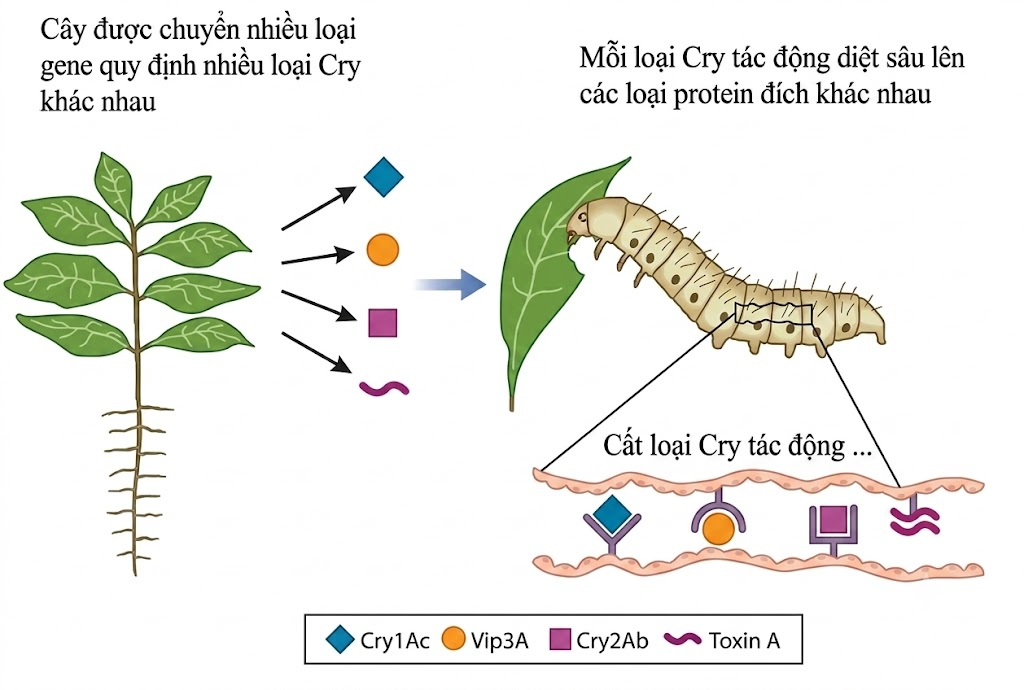
\includegraphics[width=0.7\textwidth]{image/cd_cry03_image1.png}
\end{center}
\figcaption{1}{Cơ chế diệt sâu bằng cách chuyển cùng lúc nhiều loại gene mã hóa Cry khác nhau vào cùng một loại cây trồng.}

\begin{enumerate}[leftmargin=2em, itemsep=3pt, topsep=2pt, start=3]
\item \textbf{Luân canh cây trồng và độc tố Bt:} Tránh trồng liên tục một loại cây Bt trên cùng một mảnh đất qua nhiều năm. Luân canh với các cây trồng không phải là ký chủ hoặc sử dụng các giống Bt có độc tố khác nhau. Giảm áp lực chọn lọc liên tục từ một loại độc tố duy nhất lên quần thể sâu hại.
\item \textbf{Quản lý dịch hại tổng hợp (IPM):} Kết hợp cây trồng Bt với các biện pháp kiểm soát khác như sử dụng thiên địch, thuốc trừ sâu hóa học (nếu cần thiết), và các biện pháp canh tác (làm đất, quản lý tàn dư thực vật). Giảm sự phụ thuộc tuyệt đối vào công nghệ Bt và kiểm soát sâu hại một cách bền vững hơn.
\end{enumerate}

Bằng cách áp dụng đồng bộ các biện pháp trên, nông dân có thể bảo vệ hiệu quả của công nghệ Bt, kéo dài vòng đời sản phẩm và đảm bảo an ninh lương thực một cách bền vững.

\hfill\textbf{Nguồn: Thầy Đào Anh Phúc biên soạn}
\end{readingpassage}
\vspace{2pt}
% ── CÂU HỎI CĐ 3 ──

% === Câu 1: Trắc nghiệm ===
\question[Trắc nghiệm]{Từ năm nào các gene mã hóa protein Cry bắt đầu được sử dụng để chuyển vào cây trồng?}
\par\vspace{4pt}
\noindent\choiceitem{A}{1990.}\hfill\choiceitem{B}{1992.}\hfill\choiceitem{C}{1996.}\hfill\choiceitem{D}{2000.}

% === Câu 2: Trắc nghiệm ===
\question[Trắc nghiệm]{Diện tích cây trồng Bt trên toàn cầu tính đến năm 2016 là:}
\par\vspace{4pt}
\noindent\hangindent=2.2em\hangafter=1\choiceitem{A}{Hơn 150 triệu hecta.}\par\vspace{4pt}
\noindent\hangindent=2.2em\hangafter=1\choiceitem{B}{Hơn 185 triệu hecta.}\par\vspace{4pt}
\noindent\hangindent=2.2em\hangafter=1\choiceitem{C}{Hơn 200 triệu hecta.}\par\vspace{4pt}
\noindent\hangindent=2.2em\hangafter=1\choiceitem{D}{Hơn 250 triệu hecta.}\par\vspace{4pt}

% === Câu 3: Trắc nghiệm ===
\question[Trắc nghiệm]{Lợi ích kinh tế của cây trồng Bt bao gồm:}
\par\vspace{4pt}
\noindent\hangindent=2.2em\hangafter=1\choiceitem{A}{Tăng năng suất 15--20\%, giảm sử dụng thuốc trừ sâu 25--30\%.}\par\vspace{4pt}
\noindent\hangindent=2.2em\hangafter=1\choiceitem{B}{Tăng năng suất 21--25\%, giảm sử dụng thuốc trừ sâu 35--43\%.}\par\vspace{4pt}
\noindent\hangindent=2.2em\hangafter=1\choiceitem{C}{Tăng năng suất 30--35\%, giảm sử dụng thuốc trừ sâu 45--50\%.}\par\vspace{4pt}
\noindent\hangindent=2.2em\hangafter=1\choiceitem{D}{Tăng năng suất 25--30\%, giảm sử dụng thuốc trừ sâu 40--45\%.}\par\vspace{4pt}

% === Câu 4: Trắc nghiệm ===
\question[Trắc nghiệm]{Hậu quả của việc côn trùng kháng protein Cry là gì?}
\par\vspace{4pt}
\noindent\hangindent=2.2em\hangafter=1\choiceitem{A}{Tăng đa dạng sinh học trong hệ sinh thái nông nghiệp.}\par\vspace{4pt}
\noindent\hangindent=2.2em\hangafter=1\choiceitem{B}{Gây thiệt hại cho năng suất và chất lượng sản phẩm nông nghiệp.}\par\vspace{4pt}
\noindent\hangindent=2.2em\hangafter=1\choiceitem{C}{Giảm chi phí sản xuất do không cần sử dụng thuốc trừ sâu.}\par\vspace{4pt}
\noindent\hangindent=2.2em\hangafter=1\choiceitem{D}{Cải thiện chất lượng đất canh tác.}\par\vspace{4pt}

% === Câu 5: Ghép đôi ===
\question[Ghép đôi]{Ghép đôi giữa các cơ chế kháng độc tố với đặc điểm tương ứng.}

\vspace{6pt}
\setstretch{1.3}

\textit{Cột B:}
\vspace{-6pt}
\par\vspace{4pt}
\noindent\hangindent=2.2em\hangafter=1\choiceitem{A}{Tăng khả năng phục hồi tổn thương}\par\vspace{4pt}
\noindent\hangindent=2.2em\hangafter=1\choiceitem{B}{Tránh ăn mô có độc tố cao}\par\vspace{4pt}
\noindent\hangindent=2.2em\hangafter=1\choiceitem{C}{Độc tố mất khả năng gắn kết}\par\vspace{4pt}
\noindent\hangindent=2.2em\hangafter=1\choiceitem{D}{Tạo enzyme phân giải độc tố}\par\vspace{4pt}

\vspace{6pt}

\renewcommand{\arraystretch}{1.6}
{\small\setstretch{1.0}
\begin{longtable}{|>{\raggedright\arraybackslash}m{0.55\textwidth}|>{\centering\arraybackslash}m{0.28\textwidth}|}
\hline
\rowcolor{primaryBlue!12}
\multicolumn{1}{|c|}{\cellcolor{primaryBlue!12}\textbf{Cột A}} & \cellcolor{primaryBlue!12}\textbf{Cột B} \\
\hline
\endfirsthead
\hline
\rowcolor{primaryBlue!12}
\multicolumn{1}{|c|}{\cellcolor{primaryBlue!12}\textbf{Cột A}} & \cellcolor{primaryBlue!12}\textbf{Cột B} \\
\hline
\endhead
1. Biến đổi thụ thể đích & \dropbox[2.5cm] \\
\hline
2. Thay đổi kích hoạt độc tố & \dropbox[2.5cm] \\
\hline
3. Tăng cường miễn dịch & \dropbox[2.5cm] \\
\hline
4. Cơ chế hành vi & \dropbox[2.5cm] \\
\hline
\end{longtable}
}

% === Câu 6: Trắc nghiệm ===
\question[Trắc nghiệm]{Chiến lược vùng trú ẩn (Refuge Strategy) yêu cầu bao nhiêu diện tích không phải là cây Bt?}
\par\vspace{4pt}
\noindent\choiceitem{A}{5--20\%.}\hfill\choiceitem{B}{25--30\%.}\hfill\choiceitem{C}{30--40\%.}\hfill\choiceitem{D}{40--50\%.}

% === Câu 7: Chọn nhiều đáp án ===
\question[Chọn nhiều đáp án]{Mục đích của việc tạo vùng trú ẩn là:}
\par\vspace{4pt}
\noindent\hangindent=2.2em\hangafter=1\choiceitemBox{A}{Tạo nơi sinh sống cho quần thể sâu không kháng thuốc.}\par\vspace{4pt}
\noindent\hangindent=2.2em\hangafter=1\choiceitemBox{B}{Các cá thể không kháng sẽ giao phối với cá thể kháng thuốc thiểu số.}\par\vspace{4pt}
\noindent\hangindent=2.2em\hangafter=1\choiceitemBox{C}{Tạo ra thế hệ con lai vẫn còn nhạy cảm với độc tố.}\par\vspace{4pt}
\noindent\hangindent=2.2em\hangafter=1\choiceitemBox{D}{Tăng sản lượng tổng thể của vùng canh tác.}\par\vspace{4pt}
\noindent\hangindent=2.2em\hangafter=1\choiceitemBox{E}{Giảm chi phí đầu tư vào giống cây Bt.}\par\vspace{4pt}

% === Câu 8: Trắc nghiệm ===
\question[Trắc nghiệm]{Gene xếp chồng có nghĩa là gì?}
\par\vspace{4pt}
\noindent\hangindent=2.2em\hangafter=1\choiceitem{A}{Trồng nhiều loại cây Bt khác nhau trên cùng một cánh đồng.}\par\vspace{4pt}
\noindent\hangindent=2.2em\hangafter=1\choiceitem{B}{Chuyển nhiều gene Cry vào cùng một giống cây.}\par\vspace{4pt}
\noindent\hangindent=2.2em\hangafter=1\choiceitem{C}{Xếp chồng các lớp đất để trồng cây theo từng tầng.}\par\vspace{4pt}
\noindent\hangindent=2.2em\hangafter=1\choiceitem{D}{Sắp xếp thứ tự trồng cây theo chu kỳ nhất định.}\par\vspace{4pt}

% === Câu 9: Trắc nghiệm ===
\question[Trắc nghiệm]{Để một con sâu có thể sống sót trên cây có gene xếp chồng, nó cần có điều gì?}
\par\vspace{4pt}
\noindent\hangindent=2.2em\hangafter=1\choiceitem{A}{Chỉ cần kháng một loại độc tố Cry.}\par\vspace{4pt}
\noindent\hangindent=2.2em\hangafter=1\choiceitem{B}{Có nhiều cơ chế kháng khác nhau cùng lúc.}\par\vspace{4pt}
\noindent\hangindent=2.2em\hangafter=1\choiceitem{C}{Tăng kích thước cơ thể để chống chọi.}\par\vspace{4pt}
\noindent\hangindent=2.2em\hangafter=1\choiceitem{D}{Thay đổi thời gian sinh trưởng.}\par\vspace{4pt}

% === Câu 10: Đúng/Sai ===
\question[Đúng/Sai]{Những phát biểu nào sau đây là đúng hay sai về luân canh cây trồng và độc tố Bt?}

\truefalsehead
\truefalseitem{A. Nên trồng liên tục một loại cây Bt trên cùng mảnh đất}
\truefalseitem{B. Luân canh với cây trồng không phải là ký chủ của một loại sâu}
\truefalseitem{C. Sử dụng các giống Bt có độc tố khác nhau}
\truefalseitem{D. Tăng mật độ trồng cây Bt}
\truefalseitem{E. Giảm áp lực chọn lọc lên quần thể sâu hại}
\truefalseend

% === Câu 11: Chọn nhiều đáp án ===
\question[Chọn nhiều đáp án]{Quản lý dịch hại tổng hợp (IPM) bao gồm việc kết hợp cây trồng Bt với các biện pháp nào?}
\par\vspace{4pt}
\noindent\hangindent=2.2em\hangafter=1\choiceitemBox{A}{Sử dụng thiên địch.}\par\vspace{4pt}
\noindent\hangindent=2.2em\hangafter=1\choiceitemBox{B}{Thuốc trừ sâu hóa học (nếu cần thiết).}\par\vspace{4pt}
\noindent\hangindent=2.2em\hangafter=1\choiceitemBox{C}{Các biện pháp canh tác như làm đất.}\par\vspace{4pt}
\noindent\hangindent=2.2em\hangafter=1\choiceitemBox{D}{Quản lý tàn dư thực vật.}\par\vspace{4pt}
\noindent\hangindent=2.2em\hangafter=1\choiceitemBox{E}{Tăng mật độ trồng cây Bt.}\par\vspace{4pt}
\noindent\hangindent=2.2em\hangafter=1\choiceitemBox{F}{Sử dụng phân bón hóa học nhiều hơn.}\par\vspace{4pt}

% === Câu 12: Đúng/Sai ===
\question[Đúng/Sai]{Những phát biểu nào sau đây là đúng hay sai về các phương pháp ngăn ngừa và giảm thiểu khả năng tạo ra chủng sâu kháng protein Cry?}

\truefalsehead
\truefalseitem{A. Chiến lược vùng trú ẩn tạo điều kiện cho sâu không kháng Cry sống trên đồng ruộng}
\truefalseitem{B. Chiến lược vùng trú ẩn tạo điều kiện cho sâu kháng protein Cry sinh sản với sâu không kháng protein Cry}
\truefalseitem{C. Chiến lược vùng trú ẩn làm giảm khả năng sinh sản giữa 2 côn trùng mang gene kháng protein Cry}
\truefalseitem{D. Chiến lược vùng trú ẩn sẽ không tạo ra đời con mang gene kháng thuốc}
\truefalseitem{E. Chiến lược vùng trú ẩn là chiến lược chấp nhận thiệt hại ở mức thấp nhất}
\truefalseitem{F. Cây trồng có gene xếp chồng làm giảm khả năng sống sót của cá thể mang gene kháng một loại Cry}
\truefalseitem{G. Cây trồng có gene xếp chồng có thể là động lực để hình thành nên loài sâu kháng cùng một lúc nhiều loại Cry}
\truefalseitem{H. Luân canh cây trồng và độc tố Bt làm ngắt quãng sự phát triển của quần thể sâu kháng protein Cry}
\truefalseitem{I. Quản lý dịch hại tổng hợp (IPM) là phương pháp kiểm soát sâu hại bền vững và giảm thiểu phụ thuộc vào giống cây Bt}
\truefalseend


\newpage
\begin{center}
\begin{tikzpicture}
    \node[fill=primaryBlue, rounded corners=10pt,
          inner xsep=25pt, inner ysep=14pt,
          drop shadow={shadow xshift=2pt, shadow yshift=-2pt, opacity=0.3},
          text width=14cm, align=center]
    {%
        \color{white}\fontsize{22}{28}\selectfont\bfseries
\phantomsection\label{b2_chuyende2}
        Chuyên đề 2:\\Phospholipid -- NanoMedicine%
    };
\end{tikzpicture}
\end{center}

\vspace{-8pt}

% ─────────────────────────────────────────────────────────────
% CHỦ ĐỀ 1: PHOSPHOLIPID: CẤU TẠO, PHÂN LOẠI VÀ CÁC DẠNG
%            TỰ LẮP RÁP TRONG NƯỚC
% ─────────────────────────────────────────────────────────────
\setcounter{qcounter}{0}

\phantomsection\label{b2_cd2_1}
\begin{topicbox}{\large CHỦ ĐỀ 1: PHOSPHOLIPID: CẤU TẠO, PHÂN LOẠI VÀ CÁC DẠNG TỰ LẮP RÁP TRONG NƯỚC}
\vspace{8pt}
\textit{Đọc đoạn văn sau và trả lời các câu hỏi.}
\vspace{6pt}
\end{topicbox}

\begin{readingpassage}[]

\setstretch{1.3}
Phospholipid là phân tử phân cực, không tan trong nước nhưng chúng cũng không tách hẳn ra khỏi nước thành lớp như dầu ăn. Khi được thả vào nước, hàng triệu phân tử phospholipid tự tổ chức thành các cấu trúc có hình dạng chính xác đến mức trở thành nền cho toàn bộ sự sống trên Trái Đất. Nguồn gốc của khả năng đó nằm ngay trong cấu tạo phân tử.

Mỗi phospholipid được xây trên một khung glycerol ba carbon. Khung glycerol có hai carbon (sn-1, sn-2) liên kết ester với hai chuỗi acid béo có tính kỵ nước; carbon thứ ba (sn-3) nối với một nhóm phosphate, và nhóm phosphate lại nối với một phân tử phân cực (head group) có tính ưa nước như choline, ethanolamine, serine hay inositol (Hình 1).

\vspace{2pt}
\begin{center}
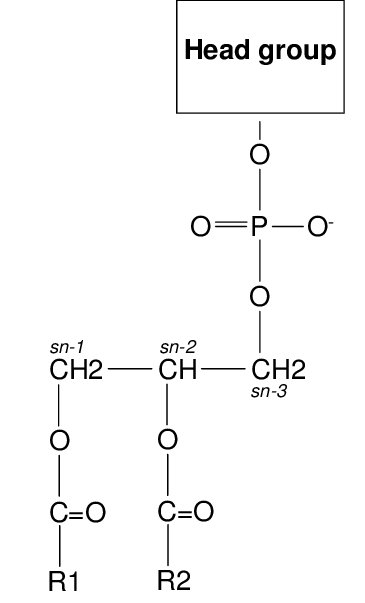
\includegraphics[width=0.30\textwidth]{image/cd_pl10_image1.png}
\end{center}
\figcaption{1}{Cấu trúc tổng thể phân tử phospholipid (a) và mô hình hóa phân tử phospholipid (b)}

Chính sự tồn tại đồng thời của đầu ưa nước và đuôi kỵ nước trong cùng một phân tử tạo nên tính lưỡng cực (amphipathic) -- gốc rễ của mọi hình thái tự lắp ráp trong nước.

Có thể dựa vào phân tử liên kết với nhóm phosphate ở phần đầu (ưa nước) để quyết định phân loại phospholipid. Bảng 1 dưới đây liệt kê bốn phospholipid dạng glycerol phổ biến ở màng tế bào động vật.

\vspace{2pt}
\tablecaption{1}{Phân loại phospholipid glycerol theo đầu phân cực}
\begin{center}
\renewcommand{\arraystretch}{1.4}
{\small
\setstretch{1.0}%
\begin{center}
\begin{tabular}{|>{\centering\arraybackslash}p{0.13\textwidth}|>{\centering\arraybackslash}p{0.16\textwidth}|>{\centering\arraybackslash}p{0.20\textwidth}|>{\raggedright\arraybackslash}p{0.35\textwidth}|}
\hline
\rowcolor{primaryBlue!12}
\textbf{Ký hiệu} & \textbf{Đầu phân cực} & \textbf{Điện tích tổng (pH 7)} & \textbf{Đặc điểm hình học phần đầu} \\
\hline
PC & Choline & 0 (zwitterion) & Đầu lớn, phân tử gần hình trụ \\
\hline
PE & Ethanolamine & 0 (zwitterion) & Đầu nhỏ, phân tử gần hình nón \\
\hline
PS & Serine & $-1$ & Đầu vừa, mang điện âm \\
\hline
PI & Inositol & $-1$ & Đầu cồng kềnh nhất, vai trò tín hiệu \\
\hline
\end{tabular}
\end{center}
}
\end{center}
\vspace{8pt}

Kích thước tương đối giữa đầu và đuôi quyết định phân tử thích ``gói'' theo hình gì khi nằm cạnh nhau. Đầu càng lớn so với đuôi, phân tử càng hình nón ngược (đầu to, đáy nhỏ); đầu và đuôi cân đối, phân tử gần hình trụ; đầu càng nhỏ so với đuôi, phân tử càng hình nón (đầu nhỏ, đáy to). Đưa những phân tử này vào nước, ba hình thái tự lắp ráp xuất hiện tùy theo tương quan hình học đó.

Micelle là một khối cầu nhỏ đường kính 3--10 nm, toàn bộ đầu ưa nước bao ngoài, toàn bộ đuôi kỵ nước gom vào tâm. Cấu trúc này chỉ ổn định khi đầu lớn hơn nhiều so với đuôi -- điển hình là acid béo tự do hay phospholipid mất một đuôi (lysophospholipid). Phospholipid nguyên chuẩn hai đuôi thường không tạo được micelle bền vì hai đuôi quá cồng kềnh để bó vào một tâm.

Liposome (vesicle) xuất hiện khi lớp bilayer tự bẻ cong và khép lại thành một cầu rỗng -- đường kính từ 30 nm đến vài µm -- bên trong là một khoang nước bị ngăn cách hoàn toàn với nước bên ngoài bằng đúng hai lớp phân tử. Khoang này chính là tiền đề cho một tế bào sơ khai có ``bên trong'' khác ``bên ngoài''.

Bilayer (lớp kép) hình thành khi hình học phân tử gần trụ: hai lớp phospholipid xếp đối nhau, đuôi hướng vào giữa để tránh nước, hai lớp đầu ưa nước phơi ra hai mặt tiếp xúc với nước. Lớp kép dày khoảng 4--5 nm và là đơn vị cấu trúc của mọi màng sinh học. Bilayer (lớp kép) là phiên bản ``phóng to'' của liposome và là cấu tạo nền chủ đạo của màng sinh chất, màng các bào quan bên trong tế bào.

\vspace{2pt}
\begin{center}
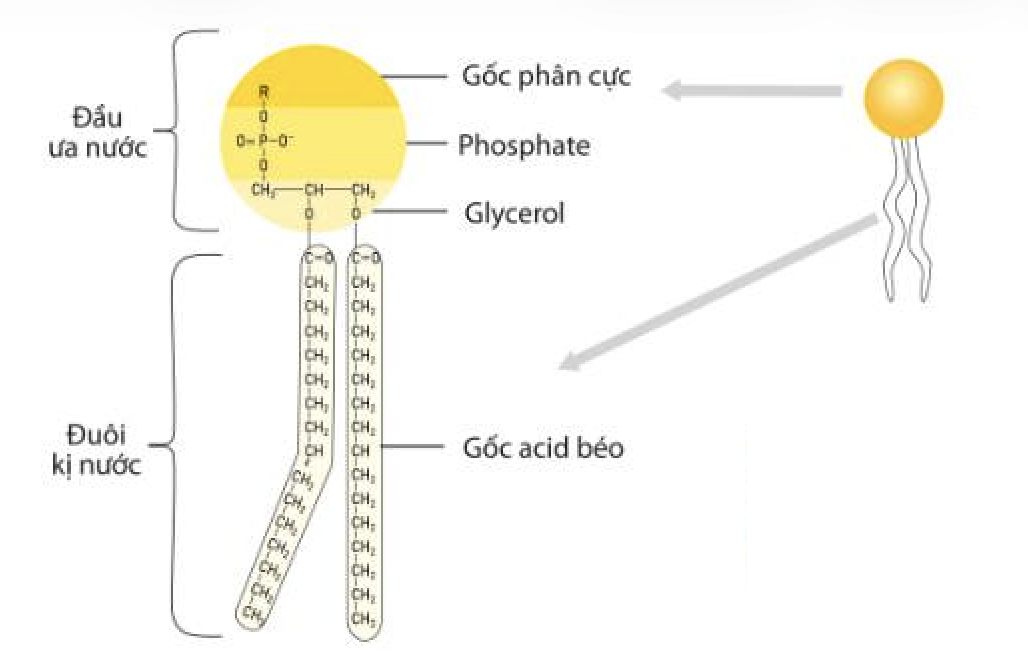
\includegraphics[width=0.7\textwidth]{image/cd_pl10_image2.png}
\end{center}
\figcaption{2}{Mô hình tập hợp của phospholipid ở trong nước: lớp kép (bilayer), micelle, liposome}
\vspace{2pt}

\tablecaption{2}{So sánh ba hình thái tự lắp ráp của phospholipid trong nước}
\begin{center}
\renewcommand{\arraystretch}{1.4}
{\small
\setstretch{1.0}%
\begin{center}
\begin{tabular}{|>{\centering\arraybackslash}p{0.14\textwidth}|>{\centering\arraybackslash}p{0.22\textwidth}|>{\centering\arraybackslash}p{0.18\textwidth}|>{\raggedright\arraybackslash}p{0.30\textwidth}|}
\hline
\rowcolor{primaryBlue!12}
\textbf{Hình thái} & \textbf{Kích thước điển hình} & \textbf{Có khoang nước bên trong} & \textbf{Điều kiện hình học phân tử} \\
\hline
Micelle & đường kính tổng thể 3--10 nm & Không & Đầu >> đuôi (thường 1 đuôi) \\
\hline
Bilayer & dày của màng 4--5 nm & Không & Đầu $\approx$ đuôi (2 đuôi cân đối) \\
\hline
Liposome & đường kính tổng thể 30 nm -- vài µm & Có & Bilayer đủ dẻo để bẻ cong khép kín \\
\hline
\end{tabular}
\end{center}
}
\end{center}
\vspace{8pt}

Vậy phospholipid không cần chọn giữa tan hoặc tách -- nó chọn tự sắp xếp, và mỗi hình thái đều là hệ quả tất yếu của tương quan hình học giữa hai vùng đối lập trong cùng một phân tử.

\hfill\textbf{Nguồn: Thầy Đào Anh Phúc biên soạn}
\end{readingpassage}
\vspace{2pt}
% ── CÂU HỎI ──

% === Câu 1: Trắc nghiệm ===
\question[Trắc nghiệm]{Dựa vào thông tin về cấu tạo phân tử, carbon thứ ba (sn-3) của khung glycerol trong phân tử phospholipid liên kết trực tiếp với thành phần nào dưới đây?}
\par\vspace{4pt}
\noindent\hangindent=2.2em\hangafter=1\choiceitem{A}{Hai chuỗi acid béo có tính kỵ nước.}\par\vspace{4pt}
\noindent\hangindent=2.2em\hangafter=1\choiceitem{B}{Nhóm phosphate.}\par\vspace{4pt}
\noindent\hangindent=2.2em\hangafter=1\choiceitem{C}{Phân tử phân cực (như choline).}\par\vspace{4pt}
\noindent\hangindent=2.2em\hangafter=1\choiceitem{D}{Một khung glycerol liền kề.}\par\vspace{4pt}

% === Câu 2: Kéo thả ===
\question[Kéo thả]{Kéo các cụm từ thích hợp vào chỗ trống để tóm tắt về sự tự lắp ráp của phospholipid.
\vspace{-4pt}
\dragitems{
\centering
    \dragitem{micelle} \dragitem{liposome} \dragitem{khoang nước}\\[1pt]
    \dragitem{acid béo} \dragitem{bilayer}
}
\setstretch{1.4}
Đưa những phân tử phospholipid vào nước, ba hình thái tự lắp ráp xuất hiện tùy theo tương quan hình học. Nếu phần đầu ưa nước lớn hơn nhiều so với đuôi kỵ nước, phân tử tập hợp thành khối cầu nhỏ gọi là (1)\,\dropbox[2cm]. Nếu phân tử cân đối gần hình trụ, chúng xếp đối nhau tạo thành (2)\,\dropbox[2cm] có bề dày 4--5 nm. Khi lớp kép này tự bẻ cong và khép kín lại thành một cầu rỗng, nó tạo ra (3)\,\dropbox[2cm]. Đặc điểm quan trọng nhất của cấu trúc khép kín này là chứa một (4)\,\dropbox[2cm] bị ngăn cách hoàn toàn với nước bên ngoài bằng đúng hai lớp phân tử, tạo nền tảng cho sự hình thành tế bào.

\vspace{2pt}
}

% === Câu 3: Trắc nghiệm ===
\question[Trắc nghiệm]{Dựa vào Bảng 1 về sự phân loại phospholipid glycerol, phân tử nào dưới đây có dạng hình học gần với hình nón nhất (đầu nhỏ, đáy to) do kích thước của đầu phân cực?}
\par\vspace{4pt}
\noindent\hangindent=2.2em\hangafter=1\choiceitem{A}{PC (phosphatidylcholine).}\par\vspace{4pt}
\noindent\hangindent=2.2em\hangafter=1\choiceitem{B}{PE (phosphatidylethanolamine).}\par\vspace{4pt}
\noindent\hangindent=2.2em\hangafter=1\choiceitem{C}{PS (phosphatidylserine).}\par\vspace{4pt}
\noindent\hangindent=2.2em\hangafter=1\choiceitem{D}{PI (phosphatidylinositol).}\par\vspace{4pt}

% === Câu 4: Ghép đôi ===
\question[Ghép đôi]{Ghép các thành phần cấu tạo của phân tử/mô hình phospholipid (Cột A) với đặc tính hoặc vai trò tương ứng (Cột B) dựa vào sơ đồ Hình 1 và văn bản.}

\vspace{6pt}
\setstretch{1.3}

\textit{Cột B:}
\vspace{-6pt}
\par\vspace{4pt}
\noindent\hangindent=2.2em\hangafter=1\choiceitem{A}{Nối trực tiếp giữa carbon thứ ba (sn-3) của glycerol và phân tử phân cực.}\par\vspace{4pt}
\noindent\hangindent=2.2em\hangafter=1\choiceitem{B}{Là đơn vị cấu trúc của mọi màng sinh học, hình thành khi đầu và đuôi cân đối.}\par\vspace{4pt}
\noindent\hangindent=2.2em\hangafter=1\choiceitem{C}{Đóng vai trò là cái khung ba carbon (sn-1, sn-2, sn-3) liên kết các thành phần của phân tử.}\par\vspace{4pt}
\noindent\hangindent=2.2em\hangafter=1\choiceitem{D}{Có tính kỵ nước, có xu hướng gom vào tâm hoặc hướng vào giữa để tránh nước.}\par\vspace{4pt}
\noindent\hangindent=2.2em\hangafter=1\choiceitem{E}{Được cấu tạo hoàn toàn từ các nhóm phân cực có kích thước cồng kềnh.}\par\vspace{4pt}
\vspace{6pt}
\renewcommand{\arraystretch}{1.6}
{\small\setstretch{1.0}
\begin{longtable}{|>{\raggedright\arraybackslash}m{0.55\textwidth}|>{\centering\arraybackslash}m{0.28\textwidth}|}
\hline
\rowcolor{primaryBlue!12}
\multicolumn{1}{|c|}{\cellcolor{primaryBlue!12}\textbf{Cột A}} & \cellcolor{primaryBlue!12}\textbf{Cột B} \\
\hline
\endfirsthead
\hline
\rowcolor{primaryBlue!12}
\multicolumn{1}{|c|}{\cellcolor{primaryBlue!12}\textbf{Cột A}} & \cellcolor{primaryBlue!12}\textbf{Cột B} \\
\hline
\endhead
1. Gốc acid béo (Đuôi kỵ nước) & \dropbox[2.5cm] \\
\hline
2. Nhóm phosphate & \dropbox[2.5cm] \\
\hline
3. Khung glycerol & \dropbox[2.5cm] \\
\hline
4. Lớp kép (Bilayer) & \dropbox[2.5cm] \\
\hline
\end{longtable}
}
}

% === Câu 5: Đúng/Sai ===
\question[Đúng/Sai]{Đánh giá tính đúng/sai của các nhận định sau về điều kiện hình thành và tính chất các cấu trúc tự lắp ráp của phospholipid trong nước:}

\truefalsehead
\truefalseitem{a) Phospholipid nguyên chuẩn hai đuôi thường khó tạo được micelle bền vững vì hai đuôi quá cồng kềnh để bó vào một tâm.}
\truefalseitem{b) Micelle là cấu trúc có đường kính từ 30 nm đến vài µm, bao bọc một lượng lớn nước ở bên trong lõi.}
\truefalseitem{c) Khoang nước bên trong liposome bị ngăn cách hoàn toàn với nước bên ngoài bởi lớp kép (bilayer) dày khoảng 4--5 nm.}
\truefalseitem{d) Sự tồn tại đồng thời của đầu ưa nước và đuôi kỵ nước trong cùng phân tử tạo nên tính lưỡng cực, là gốc rễ của mọi hình thái tự lắp ráp.}
\truefalseend
% === Câu 6: Trắc nghiệm ===
\question[Trắc nghiệm]{Một nhóm nghiên cứu y sinh muốn thiết kế một hạt liposome nhân tạo mang điện tích âm ở điều kiện sinh lý (pH 7) để tương tác chọn lọc với các thụ thể trên bề mặt tế bào khối u. Đồng thời, cấu trúc này phải là một màng lớp kép (bilayer) ổn định. Dựa vào nguyên lý tự lắp ráp và dữ liệu Bảng 1, hỗn hợp nguyên liệu nào sau đây là lựa chọn tối ưu nhất để đạt được cả hai mục tiêu này?}
\par\vspace{4pt}
\noindent\hangindent=2.2em\hangafter=1\choiceitem{A}{Sử dụng 100\% PC (phosphatidylcholine) nguyên chuẩn hai đuôi.}\par\vspace{4pt}
\noindent\hangindent=2.2em\hangafter=1\choiceitem{B}{Sử dụng hỗn hợp gồm PC (phosphatidylcholine) và PS (phosphatidylserine).}\par\vspace{4pt}
\noindent\hangindent=2.2em\hangafter=1\choiceitem{C}{Sử dụng 100\% PE (phosphatidylethanolamine).}\par\vspace{4pt}
\noindent\hangindent=2.2em\hangafter=1\choiceitem{D}{Sử dụng hỗn hợp gồm PE (phosphatidylethanolamine) và acid béo tự do.}\par\vspace{4pt}

% === Câu 7: Đúng/Sai ===
\question[Đúng/Sai]{Trong một mẻ sản xuất liposome đóng gói thuốc điều trị ung thư (thuốc dạng lỏng tan trong nước), các kĩ thuật viên phát hiện mẻ dung dịch thu được hoàn toàn không bọc được lượng thuốc nào. Quan sát dưới kính hiển vi điện tử, họ thấy hệ thống không hình thành các ``cầu rỗng'' mà chỉ tạo ra vô số các khối cầu nhỏ đặc, đường kính khoảng 5 nm. Đánh giá các giả thuyết tìm lỗi và cách khắc phục sau đây là đúng hay sai:}

\truefalsehead
\truefalseitem{a) Nguyên liệu phospholipid đã bị thủy phân mất một đuôi (thành lysophospholipid), khiến phân tử chuyển sang dạng hình nón ngược và tự lắp ráp thành micelle.}
\truefalseitem{b) Kích thước 5 nm chứng tỏ liposome đã được tạo thành nhưng khoang nước quá bé nên thuốc không chui lọt.}
\truefalseitem{c) Một nguyên nhân khác có thể do sử dụng nguyên liệu là acid béo tự do, có đầu lớn hơn nhiều so với đuôi nên không thể tạo cấu trúc màng lớp kép.}
\truefalseitem{d) Để khắc phục, cần loại bỏ lysophospholipid và sử dụng lại các phospholipid nguyên chuẩn hai đuôi có đầu và đuôi cân đối để tạo cấu trúc bilayer dẻo bẻ cong được.}
\truefalseend
% === Câu 8: Ghép đôi ===
\question[Ghép đôi]{Giả định chúng ta có thể chủ động can thiệp làm biến đổi cấu trúc và tỷ lệ hình học của một phân tử phospholipid ban đầu. Hãy ghép phương án biến đổi (Cột A) với dự đoán hệ quả tự lắp ráp dự kiến (Cột B) khi thả các phân tử này vào nước.}

\vspace{6pt}
\setstretch{1.3}

\textit{Cột B:}
\vspace{-6pt}
\par\vspace{4pt}
\noindent\hangindent=2.2em\hangafter=1\choiceitem{A}{Phân tử chuyển sang dạng hình nón (đầu nhỏ, đáy to), gây biến dạng và mất ổn định cấu trúc phẳng.}\par\vspace{4pt}
\noindent\hangindent=2.2em\hangafter=1\choiceitem{B}{Cấu trúc tự sắp xếp thành một màng đơn lớp (monolayer), trong đó các đầu ưa nước và kỵ nước đan xen.}\par\vspace{4pt}
\noindent\hangindent=2.2em\hangafter=1\choiceitem{C}{Phân tử gần hình trụ, ổn định xếp đối nhau tạo thành lớp kép (Bilayer) phơi đầu ưa nước ra tiếp xúc nước.}\par\vspace{4pt}
\noindent\hangindent=2.2em\hangafter=1\choiceitem{D}{Phân tử chuyển sang hình nón ngược (đầu to, đáy nhỏ) và bó lại tạo thành Micelle.}\par\vspace{4pt}
\vspace{6pt}
\renewcommand{\arraystretch}{1.6}
{\small\setstretch{1.0}
\begin{longtable}{|>{\raggedright\arraybackslash}m{0.55\textwidth}|>{\centering\arraybackslash}m{0.28\textwidth}|}
\hline
\rowcolor{primaryBlue!12}
\multicolumn{1}{|c|}{\cellcolor{primaryBlue!12}\textbf{Cột A}} & \cellcolor{primaryBlue!12}\textbf{Cột B} \\
\hline
\endfirsthead
\hline
\rowcolor{primaryBlue!12}
\multicolumn{1}{|c|}{\cellcolor{primaryBlue!12}\textbf{Cột A}} & \cellcolor{primaryBlue!12}\textbf{Cột B} \\
\hline
\endhead
1. Dùng enzyme cắt bỏ hoàn toàn một gốc acid béo (đuôi), khiến thể tích phần đuôi nhỏ đi rất nhiều so với đầu. & \dropbox[2.5cm] \\
\hline
2. Gắn thêm các gốc kỵ nước làm đuôi phình to gấp đôi, trong khi đầu phân cực bị thay bằng nhóm rất nhỏ. & \dropbox[2.5cm] \\
\hline
3. Giữ nguyên cấu trúc phân tử có phần đầu và hai đuôi cân đối. & \dropbox[2.5cm] \\
\hline
\end{longtable}
}
}

% === Câu 9: Điền khuyết ===
\question[Điền khuyết]{Một công ty dược thiết kế hạt nano lipid để vận chuyển một lượng lớn thuốc tan trong nước. Họ chọn hình thái tự lắp ráp là liposome. Lớp màng (bilayer) của loại liposome này có độ dày cố định là 5 nm. Tuy nhiên, để vượt qua hàng rào mạch máu quanh khối u, đường kính ngoài của liposome bị giới hạn tối đa ở mức cứng là 60 nm.\\[3pt]
\textit{(Điền từ/cụm từ (không quá 2 tiếng) hoặc số (làm tròn đến hàng đơn vị) vào chỗ trống.)}}
\vspace{2pt}
\setstretch{1.4}
\begin{itemize}[leftmargin=*, itemsep=5pt, topsep=0pt, partopsep=0pt, parsep=0pt, label=\textcolor{primaryBlue}{\textbullet}]
\item Nếu sản xuất liposome đạt đúng giới hạn kích thước ngoài 60 nm, đường kính cực đại của khoang chứa nước bên trong sẽ là (1)\,\dropbox[2cm] nm.
\item Nếu vì lý do nào đó lớp màng không khép kín được mà nguyên liệu lại bó vào một tâm sinh ra cấu trúc có đường kính chỉ khoảng 8 nm, đó là hình thái (2)\,\dropbox[2cm].
\item Số lượng khoang nước bên trong cấu trúc bị lỗi này là (3)\,\dropbox[2cm], dẫn đến việc phải loại bỏ toàn bộ mẻ thuốc vì không có không gian lưu trữ.
\end{itemize}


% ─────────────────────────────────────────────────────────────
% CHỦ ĐỀ 2: TÍNH LINH ĐỘNG CỦA MÀNG SINH CHẤT
% ─────────────────────────────────────────────────────────────
\newpage
\setcounter{qcounter}{0}

\phantomsection\label{b2_cd2_2}
\begin{topicbox}{\large CHỦ ĐỀ 2: TÍNH LINH ĐỘNG CỦA MÀNG SINH CHẤT}
\vspace{8pt}
\textit{Đọc đoạn văn sau và trả lời các câu hỏi.}
\vspace{6pt}
\end{topicbox}

\begin{readingpassage}[]

\setstretch{1.3}
Màng tế bào là màng khảm động, lớp kép phospholipid phân cực có đầu ưa nước hướng ra phía ngoài và hai đuôi kị nước hướng vào trong (Hình 1). Khi tiếp xúc với nước, tương tác ưa và kị nước làm phân tử phospholipid tự động tái lập trạng thái kép, quá trình này diễn ra không cần cung cấp năng lượng và không hình thành liên kết hóa học giữa các phân tử phospholipid. Trong lớp kép, phân tử phospholipid có thể di chuyển ngang, thay đổi khoảng cách giữa hai phân tử trong một lớp hoặc khoảng cách phân tử giữa hai lớp hoặc nhảy từ lớp này sang lớp khác. Nhờ các đặc điểm trên mà màng tế bào có tính linh động, có khả năng biến dạng hoặc dung hợp màng (Hình 2).

\vspace{2pt}
\begin{center}
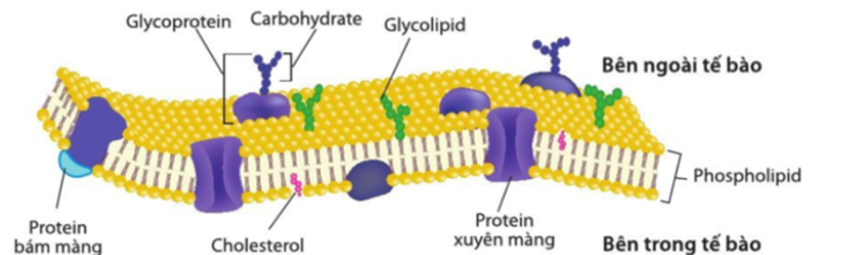
\includegraphics[width=0.7\textwidth]{image/cd_pl11_image1.png}
\end{center}
\figcaption{1}{Cấu trúc màng tế bào -- mô hình khảm động}
\vspace{2pt}

% Hình 2: 3 sub-images in tabular layout
\begin{center}
\begin{tabular}{cc}
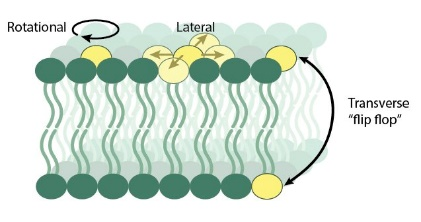
\includegraphics[width=0.42\textwidth]{image/cd_pl11_image2.jpeg} &
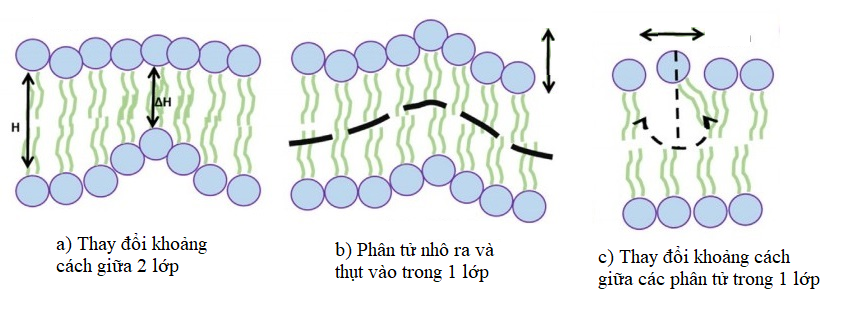
\includegraphics[width=0.42\textwidth]{image/cd_pl11_image3.png} \\[8pt]
\multicolumn{2}{c}{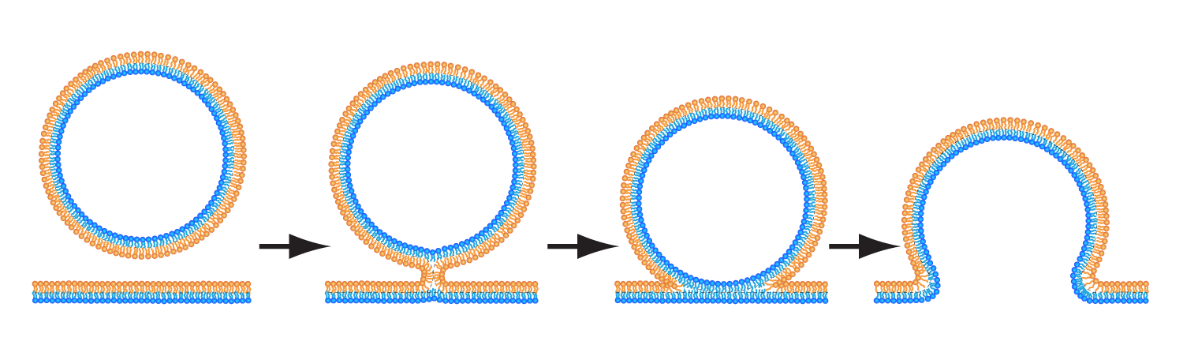
\includegraphics[width=0.50\textwidth]{image/cd_pl11_image4.png}} \\
\end{tabular}
\end{center}
\figcaption{2}{a) Các kiểu di chuyển của một phospholipid trong màng; b) Các kiểu biến dạng của lớp kép phospholipid tạo ra tính linh động; c) Diễn biến dung hợp hai lớp kép phospholipid.}

Khi màng tế bào bị ``phá vỡ'' do tác động cơ học, các phân tử phospholipid sẽ tự động tái lập trạng thái kép mà không cần có ``sự chỉ đạo'' nào của tế bào. Màng tế bào có khả năng tự động tái lập cấu trúc nhưng không có nghĩa là không thể bị phá vỡ. Ở tế bào động vật, khi tăng nhiệt độ sẽ làm phân tử phospholipid chuyển động nhanh hơn, động năng phân tử có thể lớn hơn tương tác kị nước, ưa nước dẫn đến phân tử phospholipid bị ``bắn'' vào trong nước và làm phá vỡ màng tế bào. Để ổn định cấu trúc, màng tế bào động vật có thêm hai thành phần là cholesterol (hấp thu động năng của phân tử phospholipid) và khung xương tế bào (nâng đỡ màng, giảm mức biến dạng của màng). Vì vậy, màng tế bào động vật không những có tính linh động mà còn có tính ổn định về cấu trúc.

Trong công nghệ tế bào động vật, các thao tác với tế bào ở mức micrometre không giống cách chúng ta dùng tay để giữ một quả bóng mà cần có những dụng cụ chuyên dụng. Hai loại dụng cụ chuyên dụng là micropipette và kim vi tiêm. Micropipette dùng lực hút để giữ tế bào; đường kính ống của micropipette và lực hút được thiết kế dựa vào áp lực tối thiểu có thể phá vỡ màng tế bào. Kim vi tiêm có đường kính đủ nhỏ để đâm xuyên màng tế bào và đường kính kim đủ lớn phù hợp với mục đích của thao tác (Hình 3).

\vspace{2pt}
% Hình 3: 2 sub-images side by side
\begin{center}
\begin{tabular}{cc}
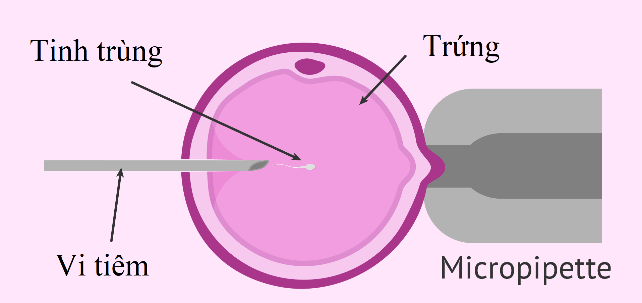
\includegraphics[width=0.42\textwidth]{image/cd_pl11_image5.png} &
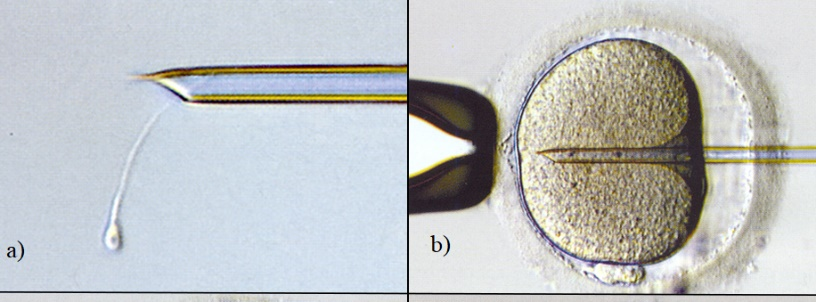
\includegraphics[width=0.42\textwidth]{image/cd_pl11_image6.jpeg} \\
\end{tabular}
\end{center}
\figcaption{3}{Kỹ thuật vi tiêm trong thụ tinh nhân tạo (IVF): (1) Mô hình tiêm tinh trùng vào trứng; (2) Hai bước thao tác: a) lấy tinh trùng vào kim vi tiêm, b) tiêm tinh trùng vào trứng đã được giữ bởi micropipette.}

\hfill\textbf{Nguồn: Thầy Đào Anh Phúc biên soạn}
\end{readingpassage}
\vspace{2pt}
% ── CÂU HỎI ──

% === Câu 1: Trắc nghiệm ===
\question[Trắc nghiệm]{Cơ chế cốt lõi nào sau đây giúp các phân tử phospholipid tự động tái lập trạng thái kép khi tiếp xúc với môi trường nước?}
\par\vspace{4pt}
\noindent\hangindent=2.2em\hangafter=1\choiceitem{A}{Hình thành các liên kết cộng hóa trị vững chắc giữa các đuôi kị nước.}\par\vspace{4pt}
\noindent\hangindent=2.2em\hangafter=1\choiceitem{B}{Tương tác ưa nước và kị nước của phân tử đối với môi trường xung quanh.}\par\vspace{4pt}
\noindent\hangindent=2.2em\hangafter=1\choiceitem{C}{Tiêu tốn năng lượng ATP của tế bào để sắp xếp các phân tử theo trật tự.}\par\vspace{4pt}
\noindent\hangindent=2.2em\hangafter=1\choiceitem{D}{Sự liên kết chặt chẽ và chỉ đạo trực tiếp của các phân tử cholesterol.}\par\vspace{4pt}

% === Câu 2: Kéo thả ===
\question[Kéo thả]{Kéo các cụm từ thích hợp vào chỗ trống để tóm tắt cơ chế bảo vệ sự ổn định của màng tế bào.
\vspace{-4pt}
\dragitems{
\centering
    \dragitem{động năng} \dragitem{kị nước} \dragitem{cholesterol} \dragitem{khung xương tế bào}\\[1pt]
    \dragitem{cộng hóa trị} \dragitem{nhiệt năng} \dragitem{liên kết hydrogen}
}
\setstretch{1.4}
Ở tế bào động vật, khi tăng nhiệt độ, các phân tử phospholipid chuyển động nhanh hơn. Nếu (1)\,\dropbox[2cm] của phân tử lớn hơn tương tác (2)\,\dropbox[2cm] và ưa nước, phân tử phospholipid có thể bị bắn ra ngoài làm màng tế bào bị phá vỡ. Để khắc phục rủi ro này, màng tế bào động vật được bổ sung thêm (3)\,\dropbox[2cm] có vai trò hấp thu động năng, và (4)\,\dropbox[2.5cm] để nâng đỡ màng, giảm mức biến dạng. Sự kết hợp này giúp màng giữ được cấu trúc linh động nhưng vẫn ổn định mà không cần hình thành liên kết (5)\,\dropbox[2cm] cứng nhắc giữa các phospholipid.

\vspace{2pt}
}

% === Câu 3: Điền khuyết ===
\question[Điền khuyết]{Trong kỹ thuật thụ tinh trong ống nghiệm (IVF), micropipette dùng lực hút để giữ tế bào trứng. Theo một phép đo giả định, áp lực tối thiểu để màng bắt đầu biến dạng và giữ được tế bào là P\textsubscript{min} = 15 kPa, còn áp lực tối đa mà màng chịu được trước khi bị phá vỡ là P\textsubscript{max} = 45 kPa. Để vừa giữ được tế bào vừa không phá vỡ màng, chuyên viên cài đặt micropipette hoạt động ở áp lực P nằm chính giữa hai giới hạn trên.\\[3pt]
\textit{(Điền từ/cụm từ (không quá 2 tiếng) hoặc số (làm tròn đến hàng đơn vị) vào chỗ trống.)}}
\vspace{2pt}
\setstretch{1.4}
Áp lực P là: \dropbox[2cm] kPa.

\vspace{2pt}

% === Câu 4: Đúng/Sai ===
\question[Đúng/Sai]{Dựa vào cấu trúc và đặc điểm của màng tế bào được mô tả trong bài đọc, các nhận định sau đây là đúng hay sai?}

\truefalsehead
\truefalseitem{a) Trong lớp kép, phân tử phospholipid có thể di chuyển ngang, thay đổi khoảng cách với phân tử bên cạnh hoặc nhảy từ lớp này sang lớp khác.}
\truefalseitem{b) Khung xương tế bào có vai trò hấp thu động năng của các phân tử phospholipid khi nhiệt độ tăng.}
\truefalseitem{c) Quá trình dung hợp màng tế bào diễn ra thuận lợi do giữa các phân tử phospholipid không có liên kết hóa học.}
\truefalseitem{d) Sự tự động tái lập trạng thái kép của màng khi bị phá vỡ đòi hỏi ``sự chỉ đạo'' trực tiếp từ tế bào.}
\truefalseend
% === Câu 5: Ghép đôi ===
\question[Ghép đôi]{Ghép các kiểu di chuyển/biến dạng của phospholipid (Cột A) với đặc điểm hoặc hệ quả tương ứng (Cột B) dựa trên Hình 2 và nội dung bài đọc (mỗi đáp án ở cột B chỉ dùng một lần).}

\vspace{6pt}
\setstretch{1.3}

\textit{Cột B:}
\vspace{-6pt}
\par\vspace{4pt}
\noindent\hangindent=2.2em\hangafter=1\choiceitem{A}{Giúp màng tế bào có khả năng biến dạng, linh động theo chiều ngang của bề mặt.}\par\vspace{4pt}
\noindent\hangindent=2.2em\hangafter=1\choiceitem{B}{Là cơ chế tạo ra sự biến dạng về độ dày (theo chiều dọc) của màng tế bào.}\par\vspace{4pt}
\noindent\hangindent=2.2em\hangafter=1\choiceitem{C}{Tế bào phải tiêu tốn năng lượng để đảo ngược đuôi kị nước ra môi trường nước.}\par\vspace{4pt}
\noindent\hangindent=2.2em\hangafter=1\choiceitem{D}{Sự dịch chuyển đòi hỏi phân tử phải đi xuyên qua vùng lõi kị nước để sang lớp đối diện.}\par\vspace{4pt}
\noindent\hangindent=2.2em\hangafter=1\choiceitem{E}{Là kiểu di chuyển giúp các phân tử đổi chỗ cho nhau trong cùng một lớp màng.}\par\vspace{4pt}
\vspace{6pt}
\renewcommand{\arraystretch}{1.6}
{\small\setstretch{1.0}
\begin{longtable}{|>{\raggedright\arraybackslash}m{0.55\textwidth}|>{\centering\arraybackslash}m{0.28\textwidth}|}
\hline
\rowcolor{primaryBlue!12}
\multicolumn{1}{|c|}{\cellcolor{primaryBlue!12}\textbf{Cột A}} & \cellcolor{primaryBlue!12}\textbf{Cột B} \\
\hline
\endfirsthead
\hline
\rowcolor{primaryBlue!12}
\multicolumn{1}{|c|}{\cellcolor{primaryBlue!12}\textbf{Cột A}} & \cellcolor{primaryBlue!12}\textbf{Cột B} \\
\hline
\endhead
1. Thay đổi khoảng cách giữa hai lớp & \dropbox[2.5cm] \\
\hline
2. Nhảy từ lớp này sang lớp khác (flip-flop) & \dropbox[2.5cm] \\
\hline
3. Thay đổi khoảng cách giữa các phân tử trong một lớp & \dropbox[2.5cm] \\
\hline
4. Di chuyển ngang trong một lớp & \dropbox[2.5cm] \\
\hline
\end{longtable}
}
}

% === Câu 6: Trắc nghiệm ===
\question[Trắc nghiệm]{Một nhóm nghiên cứu tổng hợp thành công màng liposome nhân tạo chỉ gồm lớp kép phospholipid, hoàn toàn không chứa cholesterol và khung xương tế bào. Khi tiêm liposome này vào cơ thể động vật (nhiệt độ cơ thể duy trì ở 37°C), sự cố nào sau đây có khả năng xảy ra cao nhất?}
\par\vspace{4pt}
\noindent\hangindent=2.2em\hangafter=1\choiceitem{A}{Màng liposome trở nên cứng nhắc và đóng băng hoàn toàn vì thiếu cholesterol làm trơn trượt các chuỗi acid béo.}\par\vspace{4pt}
\noindent\hangindent=2.2em\hangafter=1\choiceitem{B}{Liposome ngay lập tức hình thành các liên kết cộng hóa trị với tế bào hồng cầu trong máu để tự bảo vệ.}\par\vspace{4pt}
\noindent\hangindent=2.2em\hangafter=1\choiceitem{C}{Liposome rất dễ bị vỡ vì động năng của phospholipid tăng cao vượt tương tác kị/ưa nước mà không có thành phần hấp thu động năng.}\par\vspace{4pt}
\noindent\hangindent=2.2em\hangafter=1\choiceitem{D}{Các phân tử phospholipid tự đảo ngược đầu kị nước ra phía ngoài để tránh tác động cơ học của dòng máu.}\par\vspace{4pt}

% === Câu 7: Đúng/Sai ===
\question[Đúng/Sai]{Nghiên cứu Hình 3 về kỹ thuật vi tiêm (IVF) và các nguyên lí vật lí của màng tế bào, các nhận định sau đây đúng hay sai?}

\truefalsehead
\truefalseitem{a) Kim vi tiêm không làm hỏng tế bào vì các phân tử phospholipid bị tách ra sẽ tự động tái lập cấu trúc kép ngay sau khi rút kim nhờ tương tác ưa/kị nước.}
\truefalseitem{b) Lực hút của micropipette phải được thiết kế lớn hơn cả lực phá vỡ tương tác giữa các phân tử phospholipid để hút thật chặt tế bào.}
\truefalseitem{c) Nếu tăng nhiệt độ môi trường IVF lên quá cao, rủi ro vỡ màng trứng khi dùng kim vi tiêm sẽ tăng lên do động năng của các phân tử phospholipid tăng.}
\truefalseitem{d) Cả micropipette và kim vi tiêm đều dựa trên tính chất màng tế bào là một cấu trúc khảm tĩnh, không thay đổi vị trí các phân tử.}
\truefalseend
% === Câu 8: Điền khuyết ===
\question[Điền khuyết]{Trong công nghệ dược phẩm, việc thiết kế màng liposome nhân tạo là một bài toán.\\[3pt]
\textit{(Điền từ/cụm từ (không quá 2 tiếng) hoặc số (làm tròn đến hàng đơn vị) vào chỗ trống.)}}
\vspace{2pt}
\setstretch{1.4}
\begin{sloppypar}
\begin{itemize}[leftmargin=*, itemsep=5pt, topsep=0pt, partopsep=0pt, parsep=0pt, label=\textcolor{primaryBlue}{\textbullet}]
\item Trong công nghệ dược phẩm, việc thiết kế màng liposome nhân tạo là một bài toán (1)\,\dropbox[2cm] giữa tính linh động (giúp dung hợp màng dễ dàng để nhả thuốc) và độ ổn định (giúp màng không bị vỡ trước khi đến đích).
\item Giả sử ở 37°C, một màng liposome không có cholesterol (0\%) có khả năng dung hợp thuốc đạt 100\% nhưng tỉ lệ vỡ màng trên đường đi rất cao. Khi bổ sung cholesterol, cứ tăng thêm 1\% nồng độ cholesterol thì khả năng dung hợp giảm đi 1,5\%, nhưng màng trở nên ổn định hơn. Để đáp ứng tiêu chuẩn y tế, một màng liposome cần duy trì khả năng dung hợp chính xác ở mức 70\%. Theo quy luật tuyến tính trên, nhà sản xuất cần pha cholesterol vào màng với nồng độ là (2)\,\dropbox[2cm]\%.
\item Quyết định này giúp hấp thu bớt (3)\,\dropbox[2cm] của các phân tử phospholipid, bảo vệ màng khỏi bị vỡ do tác động cơ học của dòng máu.
\end{itemize}
\end{sloppypar}
\vspace{2pt}

% === Câu 9: Ghép đôi ===
\question[Ghép đôi]{Trong phòng thí nghiệm sinh học tế bào, sinh viên quan sát thấy các hiện tượng bất thường (Cột A) khi tác động lên các màng tế bào động vật nhân tạo. Ghép mỗi hiện tượng với nguyên nhân vật lí/hóa học cốt lõi (Cột B) gây ra nó, suy ra từ bài đọc (mỗi đáp án ở cột B chỉ dùng một lần).}

\vspace{6pt}
\setstretch{1.3}

\textit{Cột B:}
\vspace{-6pt}
\par\vspace{4pt}
\noindent\hangindent=2.2em\hangafter=1\choiceitem{A}{Màng đã hình thành các liên kết hóa học cứng nhắc, làm mất khả năng tự khép kín vốn không cần năng lượng.}\par\vspace{4pt}
\noindent\hangindent=2.2em\hangafter=1\choiceitem{B}{Màng thiếu hụt cholesterol -- thành phần hấp thu động năng dư thừa của các phân tử phospholipid.}\par\vspace{4pt}
\noindent\hangindent=2.2em\hangafter=1\choiceitem{C}{Hệ thống khung xương tế bào phát triển quá dày đặc, triệt tiêu sự thay đổi khoảng cách linh động của phospholipid.}\par\vspace{4pt}
\noindent\hangindent=2.2em\hangafter=1\choiceitem{D}{Động năng phân tử quá thấp khiến các phospholipid gần như không thể di chuyển để sắp xếp lại màng.}\par\vspace{4pt}
\noindent\hangindent=2.2em\hangafter=1\choiceitem{E}{Kiểu di chuyển nhảy lớp (flip-flop) diễn ra quá nhanh làm hỗn loạn cả hai bề mặt của màng.}\par\vspace{4pt}
\vspace{6pt}
\renewcommand{\arraystretch}{1.6}
{\small\setstretch{1.0}
\begin{longtable}{|>{\raggedright\arraybackslash}m{0.55\textwidth}|>{\centering\arraybackslash}m{0.28\textwidth}|}
\hline
\rowcolor{primaryBlue!12}
\multicolumn{1}{|c|}{\cellcolor{primaryBlue!12}\textbf{Cột A}} & \cellcolor{primaryBlue!12}\textbf{Cột B} \\
\hline
\endfirsthead
\hline
\rowcolor{primaryBlue!12}
\multicolumn{1}{|c|}{\cellcolor{primaryBlue!12}\textbf{Cột A}} & \cellcolor{primaryBlue!12}\textbf{Cột B} \\
\hline
\endhead
1. Màng vỡ tung ngay khi nhiệt độ môi trường nuôi cấy chỉ tăng nhẹ. & \dropbox[2.5cm] \\
\hline
2. Lỗ thủng sau khi vi tiêm không tự bít lại, tế bào chết dần vì dịch tế bào rò rỉ ra ngoài. & \dropbox[2.5cm] \\
\hline
3. Màng hoàn toàn mất khả năng biến dạng theo chiều ngang khi bị áp lực nhẹ từ micropipette. & \dropbox[2.5cm] \\
\hline
4. Hai tế bào không thể dung hợp màng dù đã tiếp xúc bề mặt trong thời gian dài. & \dropbox[2.5cm] \\
\hline
\end{longtable}
}
}

% === Câu 10: Trắc nghiệm ===
\question[Trắc nghiệm]{Dựa vào mô hình tương tác vật lí của màng tế bào, nếu các nhà khoa học muốn phát triển một dụng cụ ``dao vi phẫu bằng nhiệt'' để chủ động mở một lỗ nhỏ trên màng tế bào mà không cần tác động cơ học bằng kim nhọn, nguyên lí nào sau đây phù hợp với cơ chế của màng?}
\par\vspace{4pt}
\noindent\hangindent=2.2em\hangafter=1\choiceitem{A}{Chiếu tia nhiệt hội tụ cực nhỏ vào màng: nhiệt năng tăng động năng cục bộ vượt tương tác kị nước, đẩy bật phospholipid ra dung dịch và tạo lỗ thủng.}\par\vspace{4pt}
\noindent\hangindent=2.2em\hangafter=1\choiceitem{B}{Làm lạnh cực sâu một điểm trên màng để đóng băng cholesterol, khiến các liên kết cộng hóa trị giữa cholesterol và phospholipid gãy vụn thành lỗ.}\par\vspace{4pt}
\noindent\hangindent=2.2em\hangafter=1\choiceitem{C}{Bơm thật nhiều cholesterol vào một điểm trên màng để hấp thụ toàn bộ động năng, khiến phospholipid tại đó dừng chuyển động và tự rụng ra.}\par\vspace{4pt}
\noindent\hangindent=2.2em\hangafter=1\choiceitem{D}{Chiếu tia UV phá hủy hoàn toàn khung xương tế bào dưới màng, khiến màng tự nứt ra tại các vùng chứa nhiều đầu ưa nước của phospholipid.}\par\vspace{4pt}
% ─────────────────────────────────────────────────────────────
% CHỦ ĐỀ 3: NANOMEDICINE -- ỨNG DỤNG CÔNG NGHỆ NANO TRONG Y HỌC
% ─────────────────────────────────────────────────────────────
\newpage
\setcounter{qcounter}{0}

\phantomsection\label{b2_cd2_3}
\begin{topicbox}{\large CHỦ ĐỀ 3: NANOMEDICINE: ỨNG DỤNG CÔNG NGHỆ NANO TRONG Y HỌC -- HỆ VẬN CHUYỂN THUỐC LIPOSOME}
\vspace{8pt}
\textit{Đọc đoạn văn sau và trả lời các câu hỏi.}
\vspace{2pt}
\vspace{6pt}
\end{topicbox}

\begin{readingpassage}[]
\setstretch{1.3}
Ứng dụng công nghệ nano trong y học (nanomedicine) là một lĩnh vực mới và phát triển nhanh; nanomedicine là sự kết hợp giữa công nghệ nano với y sinh và dược học. Công nghệ nanomedicine thường được áp dụng để tạo ra một hệ nano vận chuyển thuốc hiệu quả, hệ này có thể là sự kết hợp của thuốc với các polymer hoặc các chất vô cơ hoặc các chất hữu cơ. Liposome là một trong những cấu tạo nano vận chuyển thuốc có thành phần là các chất hữu cơ.

Một liposome là một túi hình cầu bao gồm một màng kép phospholipid được sắp xếp xung quanh một lõi rỗng có đường kính từ 90 đến 150 nm. Vì bản chất là lớp kép phospholipid nên các liposome có thể dung hợp với nhau thành liposome có kích thước lớn hơn hoặc dung hợp với các tế bào khác (không phải là tế bào đích), kết quả làm giảm khả năng di chuyển và tác dụng của liposome. Để khắc phục nhược điểm này người ta bổ sung phân tử polyetylen glycol (PEG), PEG đóng vai trò như ``tấm ngăn'' tiếp xúc bên ngoài của liposome và cản trở sự dung hợp của lớp kép phospholipid (Hình 1). Nhờ cấu trúc lưỡng cực của màng, các thuốc ưa nước được chứa bên trong lõi rỗng của liposome, trong khi các thuốc kị nước được lồng giữ vào màng kép phospholipid.

\vspace{8pt}

\begin{center}
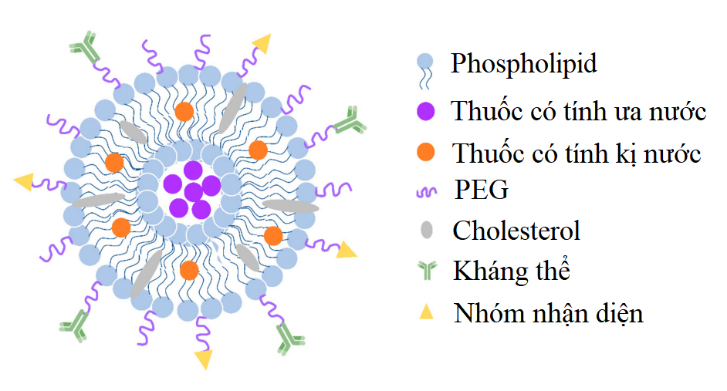
\includegraphics[width=0.7\textwidth]{image/cd_pl12_image1.png}
\end{center}
\figcaption{1}{Các thành phần cấu tạo của một liposome}

Tính đặc hiệu của liposome được quyết định bởi kháng thể và các ``nhóm nhận diện'', hai cấu tạo này giúp liposome gắn chính xác với cấu tạo chỉ có trên màng tế bào của tế bào đích mà không tác động đến các tế bào khác. Tính đặc hiệu giúp tăng hiệu quả tác động của thuốc, giảm các triệu chứng phụ làm tăng hiệu quả điều trị.

Liposome được sử dụng trong mỹ phẩm, vaccine và thuốc điều trị. Một trong những ví dụ nổi bật của công nghệ liposome là thuốc điều trị ung thư. Tế bào ung thư là những tế bào bị đột biến phân bào không ngừng. Tế bào ung thư có các biến đổi về cấu tạo màng tế bào, các quá trình sinh lí và đồng thời cũng tác động làm biến đổi cấu tạo của mao mạch tiếp xúc với nó. Khoảng hở giữa các tế bào mao mạch ở mô bình thường rất nhỏ (dưới 50 nm), trong khi ở mô chứa tế bào ung thư, khoảng hở này lớn hơn nhiều (khoảng 100 -- 800 nm). Do kích thước của phân tử thuốc rất nhỏ, nếu thuốc không được bao bọc bởi liposome thì chúng có thể xuyên qua lớp niêm mạc của mô bình thường gây thất thoát thuốc. Nhưng nếu các phân tử thuốc được bọc trong liposome thì chúng chỉ có thể đi qua khoảng hở lớn giữa các tế bào của mao mạch mô ung thư. Liposome tương tác đặc hiệu với màng tế bào ung thư, chuyển thuốc vào trong tế bào, ức chế sự phát triển và giết tế bào ung thư (Hình 2, 3).

\vspace{8pt}

\begin{center}
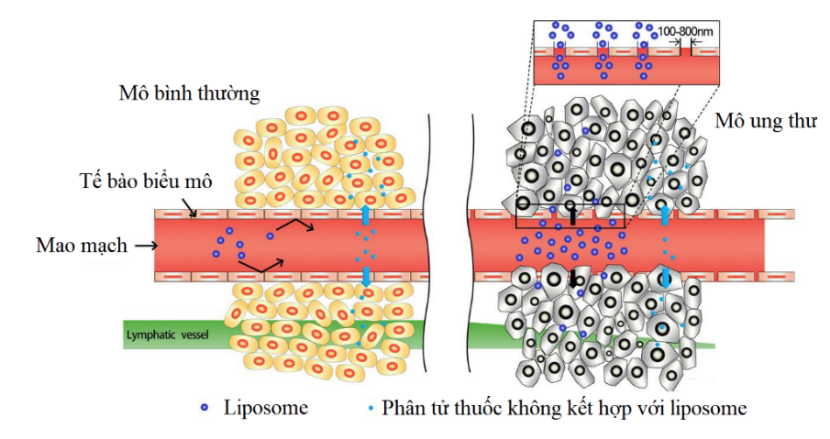
\includegraphics[width=0.7\textwidth]{image/cd_pl12_image2.png}
\end{center}
\figcaption{2}{Sự di chuyển của phân tử thuốc đơn lẻ và liposome đi qua thành mạch máu của mô bình thường và mô ung thư}
\vspace{2pt}

\begin{center}
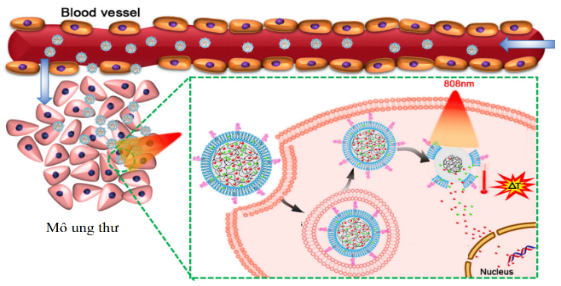
\includegraphics[width=0.7\textwidth]{image/cd_pl12_image3.png}
\end{center}
\figcaption{3}{Tác động của một loại thuốc liposome lên tế bào ung thư}

Sau khi đưa thuốc đến tế bào ung thư, liposome được đưa vào trong tế bào. Phân tử thuốc trong liposome được giải phóng tác động phá vỡ cấu trúc, rối loạn quá trình sinh lí của tế bào ung thư.

\hfill\textbf{Nguồn: Thầy Đào Anh Phúc biên soạn}
\end{readingpassage}
\vspace{2pt}
% ── CÂU HỎI ──

% === Câu 1: Trắc nghiệm ===
\question[Trắc nghiệm]{Theo nội dung bài đọc, vai trò chính của phân tử polyetylen glycol (PEG) trong cấu trúc liposome là gì?}
\par\vspace{4pt}
\noindent\hangindent=2.2em\hangafter=1\choiceitem{A}{Làm tăng khả năng gắn kết đặc hiệu của liposome vào tế bào đích.}\par\vspace{4pt}
\noindent\hangindent=2.2em\hangafter=1\choiceitem{B}{Cản trở sự dung hợp của các lớp kép phospholipid ở màng với nhau.}\par\vspace{4pt}
\noindent\hangindent=2.2em\hangafter=1\choiceitem{C}{Mở rộng khoảng hở giữa các tế bào mao mạch ở bên trong mô ung thư.}\par\vspace{4pt}
\noindent\hangindent=2.2em\hangafter=1\choiceitem{D}{Giúp hòa tan thuốc kị nước vào bên trong lõi rỗng của hạt liposome.}\par\vspace{4pt}

% === Câu 2: Ghép đôi ===
\question[Ghép đôi]{Ghép cấu trúc/thành phần của liposome (Cột A) với đặc điểm/chức năng tương ứng (Cột B).}

\vspace{6pt}
\setstretch{1.3}

\textit{Cột B:}
\vspace{-6pt}
\par\vspace{4pt}
\noindent\hangindent=2.2em\hangafter=1\choiceitem{A}{Ngăn cản sự dung hợp giữa các liposome, đóng vai trò như tấm ngăn bảo vệ màng.}\par\vspace{4pt}
\noindent\hangindent=2.2em\hangafter=1\choiceitem{B}{Trực tiếp làm màng vỏ bọc cơ bản và là không gian chứa thuốc có tính kị nước.}\par\vspace{4pt}
\noindent\hangindent=2.2em\hangafter=1\choiceitem{C}{Tạo tính đặc hiệu, giúp liposome bám chính xác vào tế bào đích mà không tác động mô lành.}\par\vspace{4pt}
\noindent\hangindent=2.2em\hangafter=1\choiceitem{D}{Là không gian rỗng chứa và vận chuyển các loại thuốc có đặc tính ưa nước.}\par\vspace{4pt}
\noindent\hangindent=2.2em\hangafter=1\choiceitem{E}{Xuyên qua các tế bào bình thường để cung cấp thuốc trực tiếp vào nhân tế bào.}\par\vspace{4pt}
\vspace{6pt}
\renewcommand{\arraystretch}{1.6}
{\small\setstretch{1.0}
\begin{longtable}{|>{\raggedright\arraybackslash}m{0.55\textwidth}|>{\centering\arraybackslash}m{0.28\textwidth}|}
\hline
\rowcolor{primaryBlue!12}
\multicolumn{1}{|c|}{\cellcolor{primaryBlue!12}\textbf{Cột A}} & \cellcolor{primaryBlue!12}\textbf{Cột B} \\
\hline
\endfirsthead
\hline
\rowcolor{primaryBlue!12}
\multicolumn{1}{|c|}{\cellcolor{primaryBlue!12}\textbf{Cột A}} & \cellcolor{primaryBlue!12}\textbf{Cột B} \\
\hline
\endhead
1. Lõi rỗng bên trong & \dropbox[2.5cm] \\
\hline
2. Kháng thể và nhóm nhận diện & \dropbox[2.5cm] \\
\hline
3. Màng kép phospholipid & \dropbox[2.5cm] \\
\hline
4. Lớp phân tử PEG & \dropbox[2.5cm] \\
\hline
\end{longtable}
}
% === Câu 3: Trắc nghiệm ===
\question[Trắc nghiệm]{Theo bài đọc, liposome hiện được sử dụng trong những lĩnh vực nào?}
\par\vspace{4pt}
\noindent\hangindent=2.2em\hangafter=1\choiceitem{A}{Mỹ phẩm, vaccine và thuốc điều trị.}\par\vspace{4pt}
\noindent\hangindent=2.2em\hangafter=1\choiceitem{B}{Chẩn đoán hình ảnh, phẫu thuật và xạ trị.}\par\vspace{4pt}
\noindent\hangindent=2.2em\hangafter=1\choiceitem{C}{Vật liệu bán dẫn, pin mặt trời và cảm biến.}\par\vspace{4pt}
\noindent\hangindent=2.2em\hangafter=1\choiceitem{D}{Dệt may, xây dựng và công nghiệp sơn.}\par\vspace{4pt}

% === Câu 4: Kéo thả ===
\question[Kéo thả]{Kéo các cụm từ thích hợp vào chỗ trống.}
\vspace{-4pt}
\dragitems{
\centering
    \dragitem{kị nước} \dragitem{ưa nước} \dragitem{đặc hiệu}\\[1pt]
    \dragitem{rộng hơn} \dragitem{hẹp hơn} \dragitem{dung hợp}
}
\setstretch{1.4}
Ứng dụng liposome làm hệ vận chuyển nano là bước tiến lớn trong y học. Nhờ có phần lõi rỗng, liposome mang theo lượng thuốc có tính (1)\,\dropbox[2cm], trong khi lớp màng kép phospholipid lại chứa thuốc (2)\,\dropbox[2cm]. Phân tử PEG bọc ngoài màng giúp cản trở hiện tượng (3)\,\dropbox[2cm] làm biến đổi kích thước hạt. Cơ chế chọn lọc mục tiêu đầu tiên mang tính vật lý là nhờ mao mạch ở mô ung thư có khoảng hở (4)\,\dropbox[2cm] mao mạch mô bình thường. Cuối cùng, liposome thể hiện cơ chế sinh học chọn lọc bằng cách gắn kết (5)\,\dropbox[2cm] lên màng tế bào ung thư đích nhờ sự hướng dẫn của các kháng thể.

\vspace{2pt}
% === Câu 5: Trắc nghiệm ===
\question[Trắc nghiệm]{Mao mạch ở mô bình thường có cấu trúc khá khít (khe hở nhỏ hơn 50 nm). Kích thước của liposome (90 -- 150 nm) đem lại lợi thế vật lý gì trong việc phân phối thuốc hóa trị?}
\par\vspace{4pt}
\noindent\hangindent=2.2em\hangafter=1\choiceitem{A}{Ngăn chặn liposome lọt qua mao mạch mô bình thường, bảo vệ tế bào khỏe mạnh.}\par\vspace{4pt}
\noindent\hangindent=2.2em\hangafter=1\choiceitem{B}{Cho phép liposome xuyên qua màng của mọi tế bào bình thường một cách an toàn.}\par\vspace{4pt}
\noindent\hangindent=2.2em\hangafter=1\choiceitem{C}{Tiêu diệt tức thì các tế bào lành có khe hở nhỏ lỡ tiếp xúc với hạt liposome.}\par\vspace{4pt}
\noindent\hangindent=2.2em\hangafter=1\choiceitem{D}{Cho phép liposome gắn đặc hiệu vào tế bào lành thay vì tế bào ung thư.}\par\vspace{4pt}

% === Câu 6: Đúng/Sai ===
\question[Đúng/Sai]{Dựa vào bài đọc, đánh giá các mệnh đề sau về cơ chế tiếp cận tế bào ung thư của hệ thống liposome là đúng hay sai:}

\truefalsehead
\truefalseitem{a) Các phân tử thuốc tự do (không bọc liposome) có thể dễ dàng đi qua và thất thoát qua lớp niêm mạc của mô bình thường.}
\truefalseitem{b) Liposome có khả năng tự thay đổi kích thước linh hoạt để đi xuyên qua mao mạch của mô bình thường một cách dễ dàng.}
\truefalseitem{c) Phần lớn các hạt liposome (90 -- 150 nm) có thể chui qua các khe hở mao mạch ở mô ung thư (100 -- 800 nm), vốn rộng hơn hẳn khe hở ở mô bình thường.}
\truefalseitem{d) Tính đặc hiệu sinh học giúp liposome tương tác và giết chết mọi tế bào nằm xung quanh mao mạch của mô ung thư.}
\truefalseend
% === Câu 7: Điền khuyết ===
\question[Điền khuyết]{Giả sử một liposome có dạng hình cầu hoàn hảo với đường kính ngoài là 120 nm. Hãy tính thể tích toàn phần của hạt liposome này theo đơn vị nm\textsuperscript{3}. Cho biết V = $\dfrac{4}{3} \times \pi \times R^3$. Lấy $\pi = 3{,}14$.}
\vspace{2pt}
\setstretch{1.4}
(Kết quả làm tròn đến phần nguyên). Kết quả: \dropbox[3cm]\,nm\textsuperscript{3}.

\vspace{2pt}
% === Câu 8: Trắc nghiệm ===
\question[Trắc nghiệm]{Trong một lô sản xuất liposome bị lỗi, lớp màng vô tình bị thiếu hụt hoàn toàn thành phần phân tử PEG. Theo cơ chế sinh học, hiện tượng nào sau đây rất có thể sẽ xảy ra làm hỏng hệ thống vận chuyển khi truyền lô thuốc này vào máu?}
\par\vspace{4pt}
\noindent\hangindent=2.2em\hangafter=1\choiceitem{A}{Các hạt nano phân tách thành vô số vi hạt để dễ dàng lọt qua mọi mao mạch.}\par\vspace{4pt}
\noindent\hangindent=2.2em\hangafter=1\choiceitem{B}{Kháng thể trên bề mặt mất đi khả năng nhận diện tế bào ung thư một cách vĩnh viễn.}\par\vspace{4pt}
\noindent\hangindent=2.2em\hangafter=1\choiceitem{C}{Các hạt liposome dung hợp tạo thành hạt quá khổ, không thể đi qua khe mao mạch.}\par\vspace{4pt}
\noindent\hangindent=2.2em\hangafter=1\choiceitem{D}{Thuốc kị nước bên trong màng di chuyển vào vùng lõi rỗng để hòa tan cùng với nước.}\par\vspace{4pt}

% === Câu 9: Ghép đôi ===
\question[Ghép đôi]{Ghép lỗi thiết kế của hệ thống liposome (Cột A) với hệ quả tương ứng (Cột B). Khe hở mao mạch mô bình thường nhỏ hơn 50 nm, khe hở mao mạch mô ung thư khoảng 100 -- 800 nm.}

\vspace{6pt}
\setstretch{1.3}

\textit{Cột B:}
\vspace{-6pt}
\par\vspace{4pt}
\noindent\hangindent=2.2em\hangafter=1\choiceitem{A}{Không lọt qua được khe hở mao mạch mô ung thư nên thuốc không đến được đích.}\par\vspace{4pt}
\noindent\hangindent=2.2em\hangafter=1\choiceitem{B}{Hệ thống mất tính đặc hiệu, không gắn chính xác vào tế bào khối u đích.}\par\vspace{4pt}
\noindent\hangindent=2.2em\hangafter=1\choiceitem{C}{Hệ thống không thể lưu giữ được thuốc kị nước trong quá trình vận chuyển.}\par\vspace{4pt}
\noindent\hangindent=2.2em\hangafter=1\choiceitem{D}{Hạt nano dễ bị lọt qua khe mao mạch mô bình thường, gây thất thoát thuốc và độc tính.}\par\vspace{4pt}
\noindent\hangindent=2.2em\hangafter=1\choiceitem{E}{Thuốc ưa nước bị buộc chuyển sang chứa bên trong màng kép phospholipid.}\par\vspace{4pt}
\vspace{6pt}
\renewcommand{\arraystretch}{1.6}
{\small\setstretch{1.0}
\begin{longtable}{|>{\raggedright\arraybackslash}m{0.55\textwidth}|>{\centering\arraybackslash}m{0.28\textwidth}|}
\hline
\rowcolor{primaryBlue!12}
\multicolumn{1}{|c|}{\cellcolor{primaryBlue!12}\textbf{Cột A}} & \cellcolor{primaryBlue!12}\textbf{Cột B} \\
\hline
\endfirsthead
\hline
\rowcolor{primaryBlue!12}
\multicolumn{1}{|c|}{\cellcolor{primaryBlue!12}\textbf{Cột A}} & \cellcolor{primaryBlue!12}\textbf{Cột B} \\
\hline
\endhead
1. Đường kính ngoài của liposome được chế tạo siêu nhỏ (dưới 40 nm). & \dropbox[2.5cm] \\
\hline
2. Không đính kèm lớp kháng thể và nhóm nhận diện lên màng ngoài. & \dropbox[2.5cm] \\
\hline
3. Đường kính ngoài của liposome được chế tạo quá lớn (khoảng 1000 nm). & \dropbox[2.5cm] \\
\hline
4. Hạt nano được tạo ra chỉ có lõi rỗng mà không có màng kép phospholipid. & \dropbox[2.5cm] \\
\hline
\end{longtable}
}
% === Câu 10: Điền khuyết ===
\question[Điền khuyết]{Điền từ/cụm từ (không quá 2 tiếng) hoặc số (làm tròn đến hàng đơn vị) vào chỗ trống:}
\vspace{2pt}
\setstretch{1.4}
Một nhóm nghiên cứu muốn nâng cấp thiết kế một liposome. Liposome ban đầu có bán kính ngoài là 70 nm, độ dày màng phospholipid là 10 nm (nghĩa là bán kính lõi rỗng là 60 nm). Nếu họ muốn chế tạo một liposome mới có thể tích phần lõi rỗng tăng lên gấp 8 lần, thì bán kính lõi rỗng mới phải đạt (1)\,\dropbox[2cm] nm. Giả sử độ dày màng phospholipid vẫn giữ nguyên là 10 nm, đường kính ngoài của hạt liposome mới sẽ là (2)\,\dropbox[2cm] nm. Đối chiếu với khoảng hở của mao mạch mô ung thư (100 -- 800 nm), hạt liposome phiên bản phóng to này (3)\,\dropbox[2cm] khả năng xâm nhập vào mô ung thư qua các khe hở mao mạch.

\vspace{2pt}
% === Câu 11: Đúng/Sai ===
\question[Đúng/Sai]{Bài toán thiết kế liposome yêu cầu các nhà khoa học phải cân nhắc (đánh đổi) giữa nhiều yếu tố. Đánh giá các định hướng tối ưu hóa:}

\truefalsehead
\truefalseitem{a) Chế tạo hạt liposome kích thước 1000 nm sẽ mang được lượng thuốc khổng lồ, đồng thời vẫn thâm nhập tốt vì mao mạch mô ung thư luôn giãn nở linh hoạt vô hạn.}
\truefalseitem{b) Để tăng nồng độ thuốc ưa nước mang theo trong một hạt liposome có đường kính ngoài cố định, nhà sản xuất bắt buộc phải tìm cách làm mỏng đi lớp màng kép phospholipid.}
\truefalseitem{c) Việc gắn quá nhiều phân tử PEG có thể tạo rào cản không gian quá dày, che khuất hoặc cản trở sự tiếp xúc của kháng thể với tế bào đích, làm giảm tính đặc hiệu.}
\truefalseitem{d) Để thâm nhập vào các khối u có khoảng hở mao mạch hẹp nhất (khoảng 100 nm), thiết kế liposome có kích thước 120 nm sẽ đem lại hiệu quả tốt hơn hạt 90 nm.}
\truefalseend
% === Câu 12: Trắc nghiệm ===
\question[Trắc nghiệm]{Một mẫu liposome thử nghiệm được chế tạo với đường kính ngoài 60 nm, có đầy đủ lớp PEG bảo vệ và kháng thể đặc hiệu với tế bào ung thư. Biết khe hở mao mạch mô bình thường nhỏ hơn 50 nm, khe hở mao mạch mô ung thư khoảng 100 -- 800 nm. Khi đưa mẫu hạt này vào cơ thể, điều gì nhiều khả năng sẽ xảy ra nhất?}
\par\vspace{4pt}
\noindent\hangindent=2.2em\hangafter=1\choiceitem{A}{Hạt thất thoát chủ yếu qua mạch máu mô bình thường và gây độc tính cho các tế bào lành.}\par\vspace{4pt}
\noindent\hangindent=2.2em\hangafter=1\choiceitem{B}{Hạt lọt vào khối u nhờ hiệu ứng qua khe hở rồi gắn đặc hiệu lên màng tế bào ung thư.}\par\vspace{4pt}
\noindent\hangindent=2.2em\hangafter=1\choiceitem{C}{Hạt không xâm nhập được cả mô lành lẫn mô ung thư nên chủ yếu lưu lại trong tuần hoàn.}\par\vspace{4pt}
\noindent\hangindent=2.2em\hangafter=1\choiceitem{D}{Hạt dung hợp với tế bào đích ngay bên trong mao mạch nhờ kháng thể đặc hiệu.}\par\vspace{4pt}

% === Câu 13: Đúng/Sai ===
\question[Đúng/Sai]{Một đội nghiên cứu đề xuất các phương án nâng cấp thiết kế liposome. Đánh giá các nhận định (cho biết V = $\dfrac{4}{3} \times \pi \times R^3$):}

\truefalsehead
\truefalseitem{a) Nếu tăng bán kính lõi rỗng lên gấp 3 lần (vẫn giữ dạng hình cầu) thì thể tích chứa thuốc ưa nước của lõi sẽ tăng lên 27 lần.}
\truefalseitem{b) Hạt liposome đường kính 105 nm vẫn lọt qua được khe hở hẹp nhất (khoảng 100 nm) của mao mạch mô ung thư.}
\truefalseitem{c) Kháng thể và nhóm nhận diện là yếu tố quyết định liposome có lọt qua được khe hở mao mạch mô ung thư hay không.}
\truefalseitem{d) Lớp PEG quá thưa thớt sẽ làm tăng nguy cơ các hạt liposome dung hợp với nhau trong quá trình vận chuyển.}
\truefalseend


% ─────────────────────────────────────────────────────────────
% CHỦ ĐỀ 4: LIPOSOME TÀNG HÌNH DOXIL
% ─────────────────────────────────────────────────────────────
\newpage
\setcounter{qcounter}{0}

\phantomsection\label{b2_cd2_4}
\begin{topicbox}{\large CHỦ ĐỀ 4: LIPOSOME TÀNG HÌNH DOXIL: GIẢI QUYẾT NGHỊCH LÝ GIỮA HIỆU QUẢ TRỊ LIỆU VÀ ĐỘC TÍNH TIM MẠCH}
\vspace{8pt}
\textit{Đọc đoạn văn sau và trả lời các câu hỏi.}
\vspace{2pt}
\vspace{6pt}
\end{topicbox}

\begin{readingpassage}[]
\setstretch{1.3}
Doxorubicin (Dox) là một trong những loại thuốc hóa trị kháng ung thư hiệu quả nhất từng được phát hiện. Phân tử này hoạt động bằng cách chèn vào chuỗi DNA, ngăn chặn sự nhân lên của tế bào ác tính. Tuy nhiên, việc sử dụng Dox trên lâm sàng gặp phải một nghịch lý lớn: Để tiêu diệt triệt để khối u, bệnh nhân cần một liều lượng lớn; nhưng nồng độ Dox cao trong máu lại gây ra độc tính không thể đảo ngược lên cơ tim (Cardiotoxicity), dẫn đến suy tim sung huyết. Giới hạn liều tích lũy tối đa an toàn của Dox tự do (Free-Dox) trong suốt cuộc đời bệnh nhân chỉ là 450 mg/m\textsuperscript{2} diện tích bề mặt cơ thể.

Để giải quyết mâu thuẫn giữa Hiệu quả trị liệu và Độc tính, các nhà khoa học đã ứng dụng công nghệ Liposome. Liposome là các túi nano hình cầu có màng lipid kép (tương tự màng tế bào người) bao bọc lấy một lõi chứa nước. Doxorubicin (tan trong nước) được giấu kín bên trong lõi này. Khi lưu thông trong máu, màng lipid bảo vệ cơ thể khỏi độc tính của thuốc.

Thế hệ Liposome đầu tiên nhanh chóng bị hệ miễn dịch (các đại thực bào) nhận diện là vật thể lạ và dọn dẹp sạch khỏi hệ tuần hoàn chỉ trong vài giờ. Giải pháp nâng cấp (thế hệ 2) là phủ lên bề mặt liposome một lớp polymer ưa nước có tên Polyethylene Glycol (PEG). Lớp PEG này tạo ra một ``đám mây không gian'' cản trở các protein miễn dịch bám vào, giúp hạt nano trở thành ``Liposome tàng hình'' (PEGylated Liposome, tên thương mại là Doxil). Nhờ vậy, thời gian bán thải của thuốc trong máu tăng lên đáng kể.

\vspace{8pt}

\begin{center}
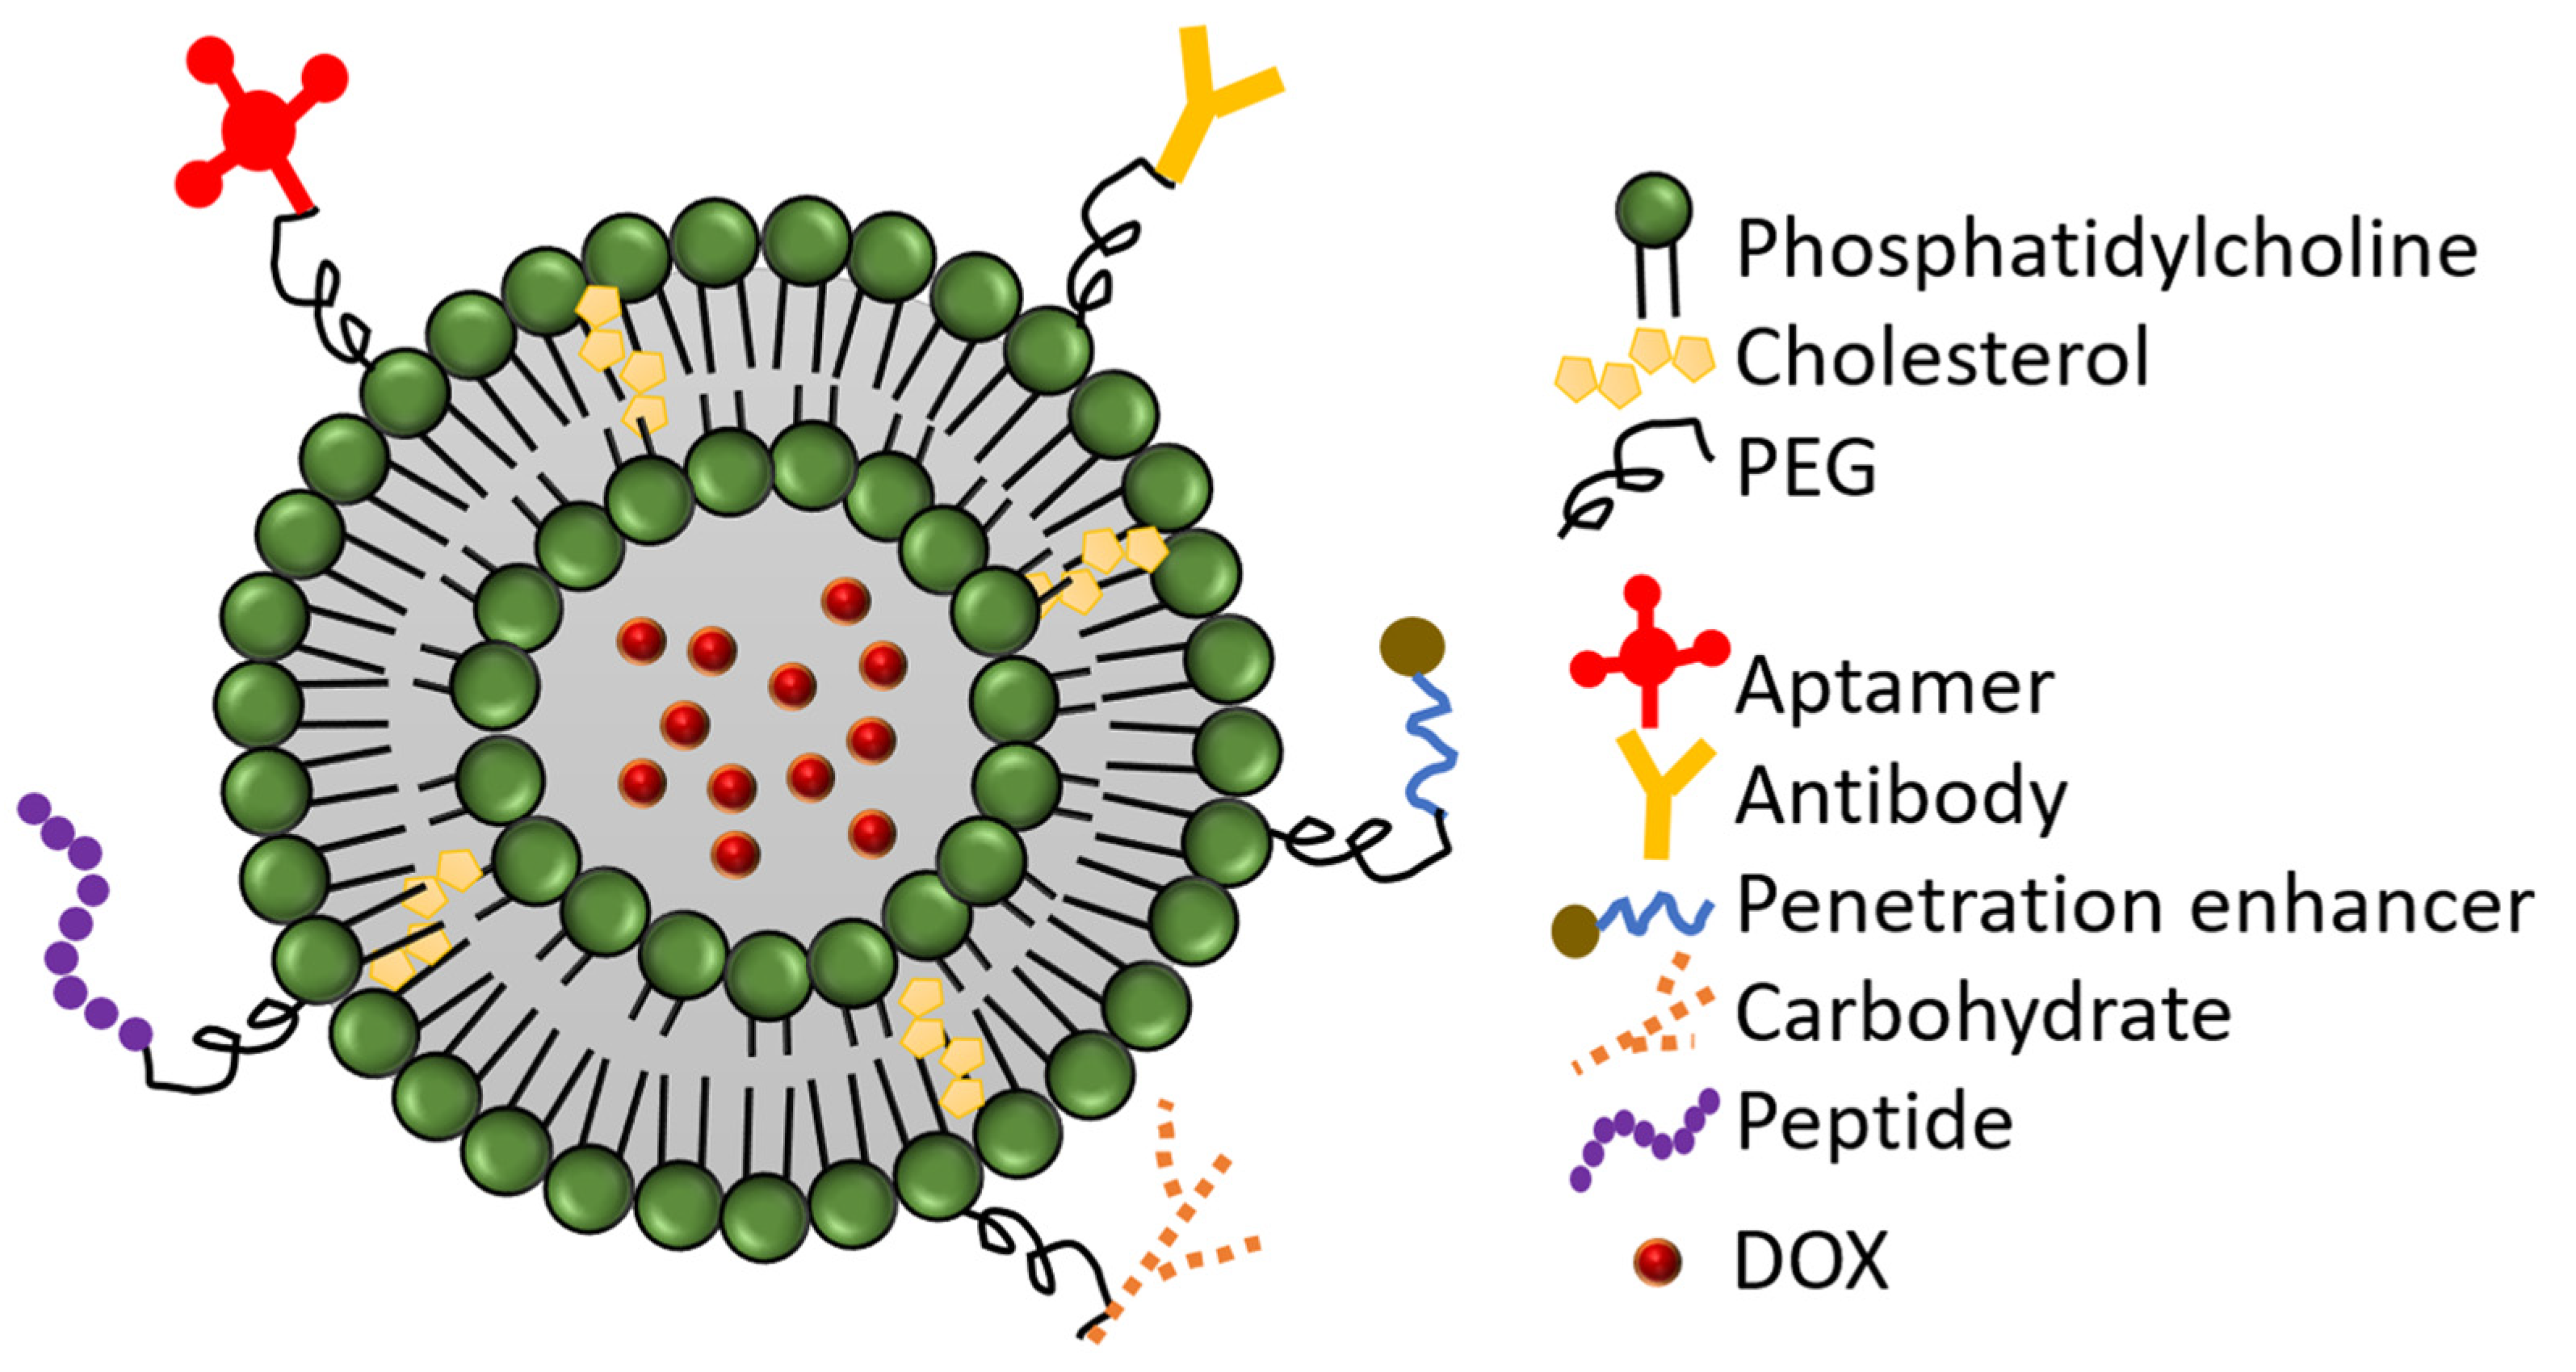
\includegraphics[width=0.55\textwidth]{image/cd_pl13_image1.png}
\end{center}
\figcaption{1}{Mô hình liposome của thuốc Doxil}

Sự tích tụ của hạt Doxil tại khối u hoàn toàn dựa vào đặc điểm sinh lý bệnh của ung thư, được gọi là Hiệu ứng EPR (Tăng tính thấm và Giữ lại). Các mạch máu mới sinh quanh khối u phát triển rất vội vã, tạo ra các khe hở lớn (kích thước 100 -- 800 nm). Hạt Doxil (kích thước khoảng 85 nm) dễ dàng lọt qua các khe hở này để xâm nhập khối u, nhưng lại quá lớn để lọt qua thành mạch máu bình thường ở tim hay da (khe hở < 10 nm).

\vspace{8pt}

\tablecaption{1}{So sánh thông số dược động học và phân bố sinh học ở động vật thực nghiệm (Sau 48 giờ tiêm)}
\begin{center}
\renewcommand{\arraystretch}{1.4}
{\small
\setstretch{1.0}%
\begin{center}
\begin{tabular}{|>{\raggedright\arraybackslash}m{0.30\textwidth}|>{\centering\arraybackslash}m{0.28\textwidth}|>{\centering\arraybackslash}m{0.28\textwidth}|}
\hline
\rowcolor{primaryBlue!12}
\textbf{Thông số đánh giá} & \textbf{Doxorubicin tự do (Free-Dox)} & \textbf{Doxil (PEGylated Liposome)} \\
\hline
Thời gian bán thải (T\textsubscript{1/2}) & Pha phân bố: 0,2 giờ; Pha thải trừ: 30 giờ & 55 giờ \\
\hline
Kích thước hạt biểu kiến & < 1 nm (phân tử nhỏ) & 85 nm \\
\hline
Nồng độ thuốc tại Khối u & 2,0 $\mu$g/g mô & 16,0 $\mu$g/g mô \\
\hline
Nồng độ thuốc tại Cơ tim & 10,0 $\mu$g/g mô & 1,0 $\mu$g/g mô \\
\hline
Giới hạn liều tích lũy tối đa & 450 mg/m\textsuperscript{2} & > 900 mg/m\textsuperscript{2} \\
\hline
\end{tabular}
\end{center}
}
\end{center}

\hfill\textbf{Nguồn: Thầy Đào Anh Phúc biên soạn}
\end{readingpassage}
\vspace{2pt}
% ── CÂU HỎI ──

% === Câu 1: Trắc nghiệm ===
\question[Trắc nghiệm]{Theo bài đọc, nghịch lý lớn nhất trong việc sử dụng Doxorubicin tự do (Free-Dox) để điều trị ung thư là gì?}
\par\vspace{4pt}
\noindent\hangindent=2.2em\hangafter=1\choiceitem{A}{Thuốc có giá thành sản xuất quá cao so với hiệu quả kéo dài sự sống.}\par\vspace{4pt}
\noindent\hangindent=2.2em\hangafter=1\choiceitem{B}{Cần dùng liều cao để diệt u nhưng lại gây độc tính không đảo ngược cho cơ tim.}\par\vspace{4pt}
\noindent\hangindent=2.2em\hangafter=1\choiceitem{C}{Thuốc dễ bị hệ miễn dịch nhận diện và đào thải ngay trước khi đến được khối u.}\par\vspace{4pt}
\noindent\hangindent=2.2em\hangafter=1\choiceitem{D}{Thuốc không thể hòa tan trong nước nên khó tiêm trực tiếp vào mạch máu.}\par\vspace{4pt}

% === Câu 2: Ghép đôi ===
\question[Ghép đôi]{Ghép các thành phần cấu trúc của hệ dẫn truyền thuốc (Cột A) với chức năng vật lý/sinh học tương ứng (Cột B).}

\vspace{6pt}
\setstretch{1.3}

\textit{Cột B:}
\vspace{-6pt}
\par\vspace{4pt}
\noindent\hangindent=2.2em\hangafter=1\choiceitem{A}{Ngăn cản sự bám dính của protein miễn dịch, kéo dài thời gian lưu thông.}\par\vspace{4pt}
\noindent\hangindent=2.2em\hangafter=1\choiceitem{B}{Tạo rào cản vật lý ngăn không cho thuốc tiếp xúc trực tiếp với cơ tim.}\par\vspace{4pt}
\noindent\hangindent=2.2em\hangafter=1\choiceitem{C}{Làm tan vỡ tế bào khối u bằng cơ chế sinh nhiệt.}\par\vspace{4pt}
\noindent\hangindent=2.2em\hangafter=1\choiceitem{D}{Khu vực lý tưởng để chứa và vận chuyển các phân tử thuốc tan trong nước.}\par\vspace{4pt}
\noindent\hangindent=2.2em\hangafter=1\choiceitem{E}{Cửa ngõ thụ động cho phép hạt nano thoát ra khỏi hệ tuần hoàn để vào u.}\par\vspace{4pt}
\vspace{6pt}
\renewcommand{\arraystretch}{1.6}
{\small\setstretch{1.0}
\begin{longtable}{|>{\raggedright\arraybackslash}m{0.55\textwidth}|>{\centering\arraybackslash}m{0.28\textwidth}|}
\hline
\rowcolor{primaryBlue!12}
\multicolumn{1}{|c|}{\cellcolor{primaryBlue!12}\textbf{Cột A}} & \cellcolor{primaryBlue!12}\textbf{Cột B} \\
\hline
\endfirsthead
\hline
\rowcolor{primaryBlue!12}
\multicolumn{1}{|c|}{\cellcolor{primaryBlue!12}\textbf{Cột A}} & \cellcolor{primaryBlue!12}\textbf{Cột B} \\
\hline
\endhead
1. Lõi chứa nước của Liposome & \dropbox[2.5cm] \\
\hline
2. Màng lipid kép & \dropbox[2.5cm] \\
\hline
3. Lớp Polyethylene Glycol (PEG) & \dropbox[2.5cm] \\
\hline
4. Khe hở mạch máu u (100 -- 800 nm) & \dropbox[2.5cm] \\
\hline
\end{longtable}
}
% === Câu 3: Đúng/Sai ===
\question[Đúng/Sai]{Dựa vào đoạn văn và Bảng 1, đánh giá tính Đúng/Sai các mệnh đề sau về mặt động học và phân bố:}

\truefalsehead
\truefalseitem{a) Do Free-Dox có kích thước phân tử rất nhỏ (< 1 nm), nó dễ dàng rò rỉ qua các mạch máu khỏe mạnh ở cơ tim (khe hở < 10 nm), dẫn đến nồng độ tích tụ tại tim cao gấp 10 lần so với Doxil.}
\truefalseitem{b) Doxil có thời gian bán thải (55 giờ) lớn hơn nhiều so với Free-Dox chứng tỏ lớp PEG đã bảo vệ hiệu quả hạt nano khỏi quá trình dọn dẹp của hệ miễn dịch.}
\truefalseitem{c) Cơ chế tiêu diệt tế bào ung thư của Doxil ưu việt hơn hẳn Free-Dox vì hoạt chất Doxorubicin trong hạt nano đã được biến đổi cấu trúc hóa học.}
\truefalseitem{d) Nồng độ Doxil tại khối u sau 48 giờ đạt 16,0 $\mu$g/g mô, cao hơn nhiều so với Free-Dox là do hiệu ứng Tăng tính thấm và Giữ lại (EPR).}
\truefalseend
% === Câu 4: Trắc nghiệm ===
\question[Trắc nghiệm]{Theo số liệu ở Bảng 1, nếu tính tỷ số giữa Nồng độ thuốc tại khối u và Nồng độ thuốc tại cơ tim (U/T), chỉ số chọn lọc này của Doxil đã được cải thiện gấp bao nhiêu lần so với Free-Dox?}
\par\vspace{4pt}
\noindent\choiceitem{A}{8 lần.}\hfill\choiceitem{B}{16 lần.}\hfill\choiceitem{C}{50 lần.}\hfill\choiceitem{D}{80 lần.}

% === Câu 5: Điền khuyết ===
\question[Điền khuyết]{Một bệnh nhân ung thư có diện tích bề mặt cơ thể là 1,6 m\textsuperscript{2}. Nếu bác sĩ chỉ định sử dụng Doxorubicin tự do (Free-Dox) theo đúng giới hạn an toàn tối đa (dữ liệu trong Bảng 1), thì tổng lượng thuốc tối đa bệnh nhân này được phép nhận trong suốt quá trình điều trị là bao nhiêu mg?}
\vspace{2pt}
\setstretch{1.4}
\textit{(Điền từ/cụm từ (không quá 2 tiếng) hoặc số (làm tròn đến hàng đơn vị) vào chỗ trống.)}\\[3pt]
Kết quả: \dropbox[3cm]\,mg.

\vspace{2pt}
% === Câu 6: Đúng/Sai ===
\question[Đúng/Sai]{Việc thiết kế lớp PEG bọc ngoài hạt Liposome là một bài toán tối ưu hóa đa mục tiêu (đánh đổi). Đánh giá các giả định sau:}

\truefalsehead
\truefalseitem{a) Nếu mật độ lớp PEG quá thưa thớt, thời gian lưu thông của hạt trong máu sẽ bị giảm sút do các đại thực bào dễ dàng tiếp cận màng lipid.}
\truefalseitem{b) Nếu gắn các chuỗi PEG quá dài và quá dày, dù kéo dài được thời gian lưu thông nhưng hạt Liposome lại khó tương tác và giải phóng thuốc vào bên trong tế bào khối u.}
\truefalseitem{c) Để tối ưu hóa tuyệt đối, chỉ cần tăng kích thước hạt Liposome lên 1000 nm để chứa được lượng thuốc khổng lồ bù trừ cho sự hao hụt.}
\truefalseitem{d) Lợi ích đánh đổi của hệ thống Doxil là chấp nhận chi phí sản xuất phức tạp hơn để nhận lại biên độ an toàn liều lượng (giới hạn tích lũy) cao gấp ít nhất hai lần.}
\truefalseend
% === Câu 7: Điền khuyết ===
\question[Điền khuyết]{Điền từ/cụm từ (không quá 2 tiếng) hoặc số (làm tròn đến hàng đơn vị) vào chỗ trống:}
\vspace{2pt}
\setstretch{1.4}
Giả sử có một nhà nghiên cứu phát triển thành công ``Hạt nano X'', có cùng đặc tính kích thước như Doxil nhưng thời gian bán thải dài hơn, đạt ngưỡng 110 giờ. Theo quy luật tỉ lệ thuận đơn giản, nếu thời gian bán thải tăng gấp đôi thì nồng độ tích lũy tại khối u sau 48 giờ cũng xấp xỉ tăng gấp đôi so với Doxil. Khi đó, nồng độ hạt X tại khối u dự kiến đạt (1)\,\dropbox[2cm] $\mu$g/g mô. Tuy nhiên, nếu một bệnh nhân sử dụng hạt X nhưng lại đồng thời sử dụng thuốc chống tạo mạch (làm thu hẹp toàn bộ khe hở mạch máu khối u xuống dưới 50 nm), lúc này hiện tượng (2)\,\dropbox[2cm] sẽ bị vô hiệu hóa hoàn toàn, khiến nồng độ hạt X tại khối u giảm về tiệm cận 0.

\vspace{2pt}
% === Câu 8: Trắc nghiệm ===
\question[Trắc nghiệm]{Trong một thử nghiệm lâm sàng, một lô thuốc Doxil được phát hiện có vấn đề về chất lượng sản xuất: Lớp PEG không bám chặt và dễ dàng bong tróc khỏi màng Liposome ngay khi vừa tiêm vào máu bệnh nhân. Hiện tượng nào sau đây là hậu quả logic nhất?}
\par\vspace{4pt}
\noindent\hangindent=2.2em\hangafter=1\choiceitem{A}{Kích thước hạt bị thu nhỏ đột ngột khiến thuốc tràn vào cơ tim gây suy tim cấp.}\par\vspace{4pt}
\noindent\hangindent=2.2em\hangafter=1\choiceitem{B}{Hạt nano mất khả năng ``tàng hình'', bị hệ miễn dịch dọn dẹp nhanh chóng khiến nồng độ tại khối u cực kỳ thấp.}\par\vspace{4pt}
\noindent\hangindent=2.2em\hangafter=1\choiceitem{C}{Doxorubicin bên trong lõi bị thay đổi cấu trúc hóa học thành một chất không có tính độc.}\par\vspace{4pt}
\noindent\hangindent=2.2em\hangafter=1\choiceitem{D}{Hiệu ứng EPR diễn ra mạnh mẽ hơn do hạt nano không bị vướng lớp PEG khi lọt qua khe hở mạch máu.}\par\vspace{4pt}

% === Câu 9: Ghép đôi ===
\question[Ghép đôi]{Ghép các sự kiện kỹ thuật/sinh lý (Cột A) với nguyên nhân sâu xa (Cột B).}

\vspace{6pt}
\setstretch{1.3}

\textit{Cột B:}
\vspace{-6pt}
\par\vspace{4pt}
\noindent\hangindent=2.2em\hangafter=1\choiceitem{A}{Mạch máu u phát triển vội vã, thiếu hoàn thiện nên xuất hiện các khe hở lớn.}\par\vspace{4pt}
\noindent\hangindent=2.2em\hangafter=1\choiceitem{B}{Các đại thực bào không có điểm tựa để gắn các thụ thể nhận diện lên bề mặt hạt.}\par\vspace{4pt}
\noindent\hangindent=2.2em\hangafter=1\choiceitem{C}{Kích thước hạt lớn hơn đường kính khe hở thành mạch mô lành lặn ở tim.}\par\vspace{4pt}
\noindent\hangindent=2.2em\hangafter=1\choiceitem{D}{Là phân tử nhỏ không được màng lipid bảo vệ nên bị cơ thể đào thải nhanh khỏi vòng tuần hoàn.}\par\vspace{4pt}
\noindent\hangindent=2.2em\hangafter=1\choiceitem{E}{Áp suất thẩm thấu tại khối u thấp hơn trong mạch máu.}\par\vspace{4pt}
\vspace{6pt}
\renewcommand{\arraystretch}{1.6}
{\small\setstretch{1.0}
\begin{longtable}{|>{\raggedright\arraybackslash}m{0.55\textwidth}|>{\centering\arraybackslash}m{0.28\textwidth}|}
\hline
\rowcolor{primaryBlue!12}
\multicolumn{1}{|c|}{\cellcolor{primaryBlue!12}\textbf{Cột A}} & \cellcolor{primaryBlue!12}\textbf{Cột B} \\
\hline
\endfirsthead
\hline
\rowcolor{primaryBlue!12}
\multicolumn{1}{|c|}{\cellcolor{primaryBlue!12}\textbf{Cột A}} & \cellcolor{primaryBlue!12}\textbf{Cột B} \\
\hline
\endhead
1. Doxil không lọt vào tế bào cơ tim. & \dropbox[2.5cm] \\
\hline
2. Free-Dox bị thải trừ nhanh chóng (T\textsubscript{1/2} pha thải trừ = 30 giờ). & \dropbox[2.5cm] \\
\hline
3. PEG giúp hạt Liposome ``tàng hình''. & \dropbox[2.5cm] \\
\hline
4. Hiệu ứng EPR tồn tại ở khối u. & \dropbox[2.5cm] \\
\hline
\end{longtable}
}
% === Câu 10: Kéo thả ===
\question[Kéo thả]{Kéo các cụm từ thích hợp vào chỗ trống.}
\vspace{-4pt}
\dragitems{
\centering
    \dragitem{chủ động} \dragitem{kích thước} \dragitem{thụ động}\\[1pt]
    \dragitem{màng lipid} \dragitem{thời gian lưu thông}
}
\setstretch{1.4}
Sự ra đời của hạt nano Doxil là minh chứng cho việc giải quyết nghịch lý độc tính trong hóa trị. Việc bọc thuốc vào (1)\,\dropbox[2.5cm] giúp cô lập độc tính, trong khi lớp PEG bề mặt giúp gia tăng (2)\,\dropbox[3cm]. Quan trọng nhất, sự nhắm đích của hệ thống này hoàn toàn mang tính (3)\,\dropbox[2cm], lợi dụng sự chênh lệch (4)\,\dropbox[2cm] giữa mạch máu mô lành và mạch máu khối u.
% ─────────────────────────────────────────────────────────────
% CHỦ ĐỀ 5: POLYMERIC MICELLE GENEXOL-PM: TỐI ƯU HÓA HỆ DẪN
%            TRUYỀN THUỐC THEO ĐIỀU KIỆN BIÊN
% ─────────────────────────────────────────────────────────────
\newpage
\setcounter{qcounter}{0}

\phantomsection\label{b2_cd2_5}
\begin{topicbox}{\large CHỦ ĐỀ 5: POLYMERIC MICELLE GENEXOL-PM: TỐI ƯU HÓA HỆ DẪN TRUYỀN THUỐC THEO ĐIỀU KIỆN BIÊN}
\vspace{8pt}
\textit{Đọc đoạn văn sau và trả lời các câu hỏi.}
\vspace{6pt}
\end{topicbox}

\begin{readingpassage}[]

\setstretch{1.3}
Paclitaxel là một trong những loại thuốc hóa trị ưu việt nhất trong điều trị ung thư vú và ung thư buồng trứng. Tuy nhiên, nhược điểm chí mạng của phân tử này là tính kỵ nước cực kỳ cao, gần như không thể hòa tan trong nước hay huyết tương. Để có thể tiêm vào tĩnh mạch, dạng bào chế truyền thống (tên thương mại Taxol) bắt buộc phải sử dụng một hỗn hợp dung môi là Cremophor EL và Ethanol. Vấn đề phát sinh là bản thân dung môi Cremophor EL lại gây ra các phản ứng dị ứng nghiêm trọng, buộc bệnh nhân phải dùng thuốc ức chế miễn dịch trước khi hóa trị.

Để giải quyết triệt để rào cản này, công nghệ nano đã sử dụng Polymeric Micelle làm hệ thống dẫn truyền (tên thương mại Genexol-PM). Micelle là các hạt nano hình cầu tự lắp ráp từ các polymer ``lưỡng tính'' (Amphiphilic block copolymers). Chẳng hạn, polymer mPEG-PLA có một đầu mPEG rất ưa nước (Hydrophilic) và một đuôi PLA cực kỳ kỵ nước (Hydrophobic). Khi ở trong môi trường nước với nồng độ đủ lớn, các đuôi PLA sẽ tự cuộn lại với nhau tạo thành một ``lõi'' kỵ nước để giấu Paclitaxel vào trong, còn các đầu mPEG bung ra ngoài tạo thành lớp vỏ ưa nước giúp toàn bộ hạt nano hòa tan hoàn hảo trong máu (Hình 1).

\vspace{2pt}
\begin{center}
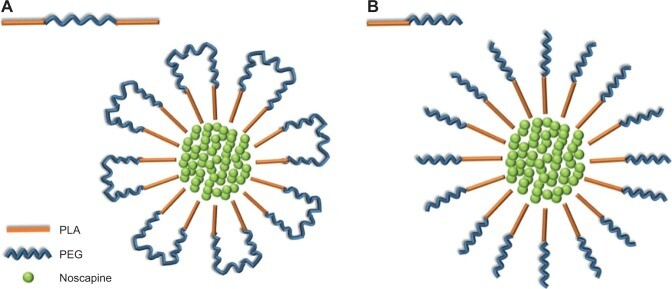
\includegraphics[width=0.7\textwidth]{image/cd_pl14_image1.png}
\end{center}
\figcaption{1}{Hai loại polymer mPEG-PLA (Loại A, B) và cấu hình Polymeric Micelle tương ứng. Phân tử thuốc nằm phía trong lõi của micelle}

Tuy nhiên, việc thiết kế hạt Micelle là một bài toán tối ưu hóa đa mục tiêu với các điều kiện biên ngặt nghèo. Quá trình tự lắp ráp chỉ xảy ra khi nồng độ polymer trong dung dịch vượt qua một ngưỡng giới hạn gọi là Nồng độ micelle tới hạn (CMC -- Critical Micelle Concentration). Nếu nồng độ polymer thấp hơn CMC, các hạt Micelle sẽ lập tức vỡ ra thành các chuỗi polymer đơn lẻ. Khi tiêm thuốc vào tĩnh mạch, thể tích máu lớn của cơ thể (khoảng 5 lít) sẽ làm pha loãng thuốc ngay lập tức. Do đó, hệ dẫn truyền cần có giá trị CMC càng thấp càng tốt để hạt Micelle không bị vỡ rã trước khi đến được khối u.

Đồng thời, cấu trúc hạt phải đảm bảo Tỷ lệ tải thuốc (DLC -- Drug Loading Capacity) đủ cao để đưa được lượng lớn hóa chất vào lõi, và kích thước hạt phải dưới 100 nm để có thể chui qua các khe hở mạch máu rò rỉ tại khối u (Hiệu ứng EPR). Việc thay đổi tỷ lệ giữa phần ưa nước (mPEG) và phần kỵ nước (PLA) sẽ làm thay đổi hoàn toàn các thông số này.

\vspace{2pt}
\tablecaption{1}{Thông số hóa lý và sinh học của các công thức bào chế Paclitaxel}
\begin{center}
\renewcommand{\arraystretch}{1.4}
{\small
\setstretch{1.0}%
\begin{center}
\begin{tabular}{|>{\raggedright\arraybackslash}p{0.22\textwidth}|>{\centering\arraybackslash}p{0.18\textwidth}|>{\centering\arraybackslash}p{0.22\textwidth}|>{\centering\arraybackslash}p{0.18\textwidth}|}
\hline
\rowcolor{primaryBlue!12}
\textbf{Thông số đánh giá} & \textbf{Taxol (Dùng dung môi Cremophor EL)} & \textbf{Genexol-PM (Micelle A -- mPEG:PLA 50:50)} & \textbf{Micelle B (mPEG:PLA 70:30)} \\
\hline
Độ hòa tan biểu kiến (mg/mL) & 0,3 & 25,0 & 40,0 \\
\hline
Kích thước hạt (nm) & Không có (Dạng dung dịch) & 25 & 15 \\
\hline
Nồng độ micelle tới hạn -- CMC (mg/L) & Không áp dụng & 2,5 & 15,0 \\
\hline
Tỷ lệ tải thuốc -- DLC (\%) & Không áp dụng & 16,7\% & 8,5\% \\
\hline
Liều dung nạp tối đa -- MTD (mg/kg) & 20 & 60 & 45 \\
\hline
\end{tabular}
\end{center}
}
\end{center}
\vspace{2pt}
{\small \textit{Ghi chú: DLC tính bằng khối lượng Paclitaxel chia cho tổng khối lượng của hạt nano.}}

\hfill\textbf{Nguồn: Thầy Đào Anh Phúc biên soạn}
\end{readingpassage}
\vspace{2pt}
% ── CÂU HỎI ──

% === Câu 1: Trắc nghiệm ===
\question[Trắc nghiệm]{Theo bài đọc, lý do chính khiến việc sử dụng thuốc Taxol truyền thống gây ra các phản ứng dị ứng nghiêm trọng cho bệnh nhân là gì?}
\par\vspace{4pt}
\noindent\hangindent=2.2em\hangafter=1\choiceitem{A}{Do kích thước hạt nano của Taxol quá lớn, làm tắc nghẽn các mạch máu.}\par\vspace{4pt}
\noindent\hangindent=2.2em\hangafter=1\choiceitem{B}{Do thành phần dung môi Cremophor EL được dùng để hòa tan thuốc.}\par\vspace{4pt}
\noindent\hangindent=2.2em\hangafter=1\choiceitem{C}{Do bản thân hoạt chất Paclitaxel tấn công trực tiếp vào hệ miễn dịch.}\par\vspace{4pt}
\noindent\hangindent=2.2em\hangafter=1\choiceitem{D}{Do nồng độ Paclitaxel trong máu vượt qua giới hạn dung nạp tối đa.}\par\vspace{4pt}

% === Câu 2: Ghép đôi ===
\question[Ghép đôi]{Ghép các thành phần cấu tạo (Cột A) với bản chất hoặc chức năng vật lý tương ứng (Cột B).}

\vspace{6pt}
\setstretch{1.3}

\textit{Cột B:}
\vspace{-6pt}
\par\vspace{4pt}
\noindent\hangindent=2.2em\hangafter=1\choiceitem{A}{Giấu và giữ chặt các phân tử thuốc hóa trị bên trong.}\par\vspace{4pt}
\noindent\hangindent=2.2em\hangafter=1\choiceitem{B}{Hướng ra ngoài để tương tác với nước, giúp hạt hòa tan.}\par\vspace{4pt}
\noindent\hangindent=2.2em\hangafter=1\choiceitem{C}{Vô hiệu hóa hệ miễn dịch để thuốc không bị đào thải.}\par\vspace{4pt}
\noindent\hangindent=2.2em\hangafter=1\choiceitem{D}{Là phần cực kỳ kỵ nước, tự cuộn lại với nhau khi vào nước.}\par\vspace{4pt}
\noindent\hangindent=2.2em\hangafter=1\choiceitem{E}{Là phân tử kỵ nước cực cao, gần như không hòa tan trong nước hay huyết tương.}\par\vspace{4pt}
\vspace{6pt}
\renewcommand{\arraystretch}{1.6}
{\small\setstretch{1.0}
\begin{longtable}{|>{\raggedright\arraybackslash}m{0.55\textwidth}|>{\centering\arraybackslash}m{0.28\textwidth}|}
\hline
\rowcolor{primaryBlue!12}
\multicolumn{1}{|c|}{\cellcolor{primaryBlue!12}\textbf{Cột A}} & \cellcolor{primaryBlue!12}\textbf{Cột B} \\
\hline
\endfirsthead
\hline
\rowcolor{primaryBlue!12}
\multicolumn{1}{|c|}{\cellcolor{primaryBlue!12}\textbf{Cột A}} & \cellcolor{primaryBlue!12}\textbf{Cột B} \\
\hline
\endhead
1. Đầu mPEG của polymer & \dropbox[2.5cm] \\
\hline
2. Đuôi PLA của polymer & \dropbox[2.5cm] \\
\hline
3. Paclitaxel nguyên bản & \dropbox[2.5cm] \\
\hline
4. Lõi của hạt Micelle & \dropbox[2.5cm] \\
\hline
\end{longtable}
}
}

% === Câu 3: Đúng/Sai ===
\question[Đúng/Sai]{Dựa vào bài đọc và Bảng 1, đánh giá tính Đúng/Sai:}

\truefalsehead
\truefalseitem{a) Cả Genexol-PM và Micelle B đều có kích thước hạt đủ nhỏ (dưới 100 nm) để tận dụng được hiệu ứng EPR tại khối u.}
\truefalseitem{b) Việc tăng tỷ lệ phần ưa nước mPEG trong cấu trúc polymer từ 50\% lên 70\% đã giúp độ hòa tan biểu kiến của thuốc tăng lên đáng kể.}
\truefalseitem{c) Liều dung nạp tối đa (MTD) của Genexol-PM cao gấp 3 lần so với Taxol là do hoạt chất Paclitaxel bên trong đã được làm giảm độc tính hóa học.}
\truefalseitem{d) Micelle B có Tỷ lệ tải thuốc (DLC) thấp hơn Micelle A là do phần lõi kỵ nước PLA bị thu hẹp lại, làm giảm không gian chứa thuốc.}
\truefalseend
% === Câu 4: Trắc nghiệm ===
\question[Trắc nghiệm]{Mặc dù công thức Micelle B mang lại khả năng hòa tan thuốc trong nước cao hơn hẳn (40,0 mg/mL), tại sao công thức Genexol-PM (Micelle A) lại là sự lựa chọn ưu việt và an toàn hơn để tiêm vào máu bệnh nhân?}
\par\vspace{4pt}
\noindent\hangindent=2.2em\hangafter=1\choiceitem{A}{Vì Micelle A có kích thước hạt 25 nm nên di chuyển trong mạch máu nhanh và ổn định hơn hẳn so với các hạt có kích thước chỉ 15 nm.}\par\vspace{4pt}
\noindent\hangindent=2.2em\hangafter=1\choiceitem{B}{Vì Micelle A có tỷ lệ tải thuốc thấp hơn nên giải phóng thuốc chậm dần, giúp cơ thể bệnh nhân tránh được sốc độc tính.}\par\vspace{4pt}
\noindent\hangindent=2.2em\hangafter=1\choiceitem{C}{Vì Micelle A có giá trị CMC thấp hơn, giúp các hạt nano khó bị vỡ cấu trúc khi bị pha loãng trong máu.}\par\vspace{4pt}
\noindent\hangindent=2.2em\hangafter=1\choiceitem{D}{Vì Micelle A sử dụng bổ sung một lượng nhỏ dung môi Cremophor EL để ổn định hệ thống hạt nano trong huyết tương.}\par\vspace{4pt}

% === Câu 5: Điền khuyết ===
\question[Điền khuyết]{Một bệnh nhân ung thư vú nặng 55 kg được chỉ định điều trị bằng Genexol-PM. Nếu sử dụng đúng theo mức Liều dung nạp tối đa (MTD) trong Bảng 1, lượng Paclitaxel tối đa mà bệnh nhân này có thể nhận trong một đợt tiêm là bao nhiêu mg?\\[3pt]
\textit{(Điền từ/cụm từ (không quá 2 tiếng) hoặc số (làm tròn đến hàng đơn vị) vào chỗ trống.)}}
\vspace{2pt}
\setstretch{1.4}
Kết quả: \dropbox[3cm] mg.

\vspace{2pt}

% === Câu 6: Đúng/Sai ===
\question[Đúng/Sai]{Một kỹ sư hóa sinh muốn thiết kế hạt ``Micelle C'' (sử dụng tỷ lệ mPEG:PLA là 90:10). Đánh giá các dự đoán:}

\truefalsehead
\truefalseitem{a) Tỷ lệ tải thuốc (DLC) của Micelle C chắc chắn sẽ vượt mức 20\% do hạt trở nên ưa nước hơn.}
\truefalseitem{b) Giá trị CMC của Micelle C sẽ rất cao, dẫn đến nguy cơ hạt nano bị vỡ tan ngay khi vừa tiêm vào dòng máu.}
\truefalseitem{c) Kích thước hạt Micelle C có xu hướng nhỏ hơn 15 nm do phần lõi chứa thuốc bị thu hẹp đáng kể.}
\truefalseitem{d) Thiết kế này vi phạm điều kiện biên về độ ổn định vật lý (Stability constraint) khi ứng dụng thực tế.}
\truefalseend
% === Câu 7: Điền khuyết ===
\question[Điền khuyết]{So sánh các công thức bào chế Paclitaxel dựa trên dữ liệu Bảng 1.\\[3pt]
\textit{(Điền từ/cụm từ (không quá 2 tiếng) hoặc số (làm tròn đến hàng đơn vị) vào chỗ trống.)}}
\vspace{2pt}
\setstretch{1.4}
So với công thức truyền thống Taxol, việc bọc Paclitaxel trong Micelle A (Genexol-PM) đã giúp tăng giới hạn độ hòa tan biểu kiến của thuốc lên xấp xỉ (1)\,\dropbox[2cm] lần, hoàn toàn giải quyết được sự phụ thuộc vào dung môi độc hại. Ở khía cạnh năng lực bào chế, giả sử nhà máy sản xuất thu được 100 gam bột hạt nano Genexol-PM thành phẩm, khối lượng hoạt chất Paclitaxel nguyên chất thực sự nằm bên trong lô hàng này là (2)\,\dropbox[2cm] gam. Nếu họ chuyển sang sản xuất 100 gam hạt Micelle B, khối lượng polymer (phần vỏ không mang dược tính) họ phải sử dụng sẽ chiếm tới (3)\,\dropbox[2cm] gam.

\vspace{2pt}

% === Câu 8: Trắc nghiệm ===
\question[Trắc nghiệm]{Trong một phòng thí nghiệm, khi nhỏ dung dịch chứa Micelle A vào một bồn mô phỏng dòng máu, các cảm biến quang học phát hiện dung dịch đột ngột chuyển từ trạng thái trong suốt sang đục ngầu, xuất hiện các tinh thể chất rắn siêu nhỏ nổi lơ lửng. Nguyên nhân kỹ thuật nào sau đây giải thích đúng nhất?}
\par\vspace{4pt}
\noindent\hangindent=2.2em\hangafter=1\choiceitem{A}{Nhiệt độ của bồn mô phỏng quá cao khiến phần mPEG bị biến tính và vỡ ra.}\par\vspace{4pt}
\noindent\hangindent=2.2em\hangafter=1\choiceitem{B}{Dung dịch bị pha loãng vượt quá giới hạn, khiến nồng độ polymer tụt xuống dưới mức CMC.}\par\vspace{4pt}
\noindent\hangindent=2.2em\hangafter=1\choiceitem{C}{Hiệu ứng EPR diễn ra quá mạnh làm các hạt nano kết tụ lại với nhau thành tinh thể.}\par\vspace{4pt}
\noindent\hangindent=2.2em\hangafter=1\choiceitem{D}{Lõi PLA của hạt hấp thụ nước từ bồn mô phỏng, đẩy toàn bộ thuốc ra ngoài lớp vỏ.}\par\vspace{4pt}

% === Câu 9: Ghép đôi ===
\question[Ghép đôi]{Ghép các thông số vật lý (Cột A) với ý nghĩa lâm sàng/bào chế tương ứng (Cột B).}

\vspace{6pt}
\setstretch{1.3}

\textit{Cột B:}
\vspace{-6pt}
\par\vspace{4pt}
\noindent\hangindent=2.2em\hangafter=1\choiceitem{A}{Quyết định khả năng hạt thoát mạch, xâm nhập vào khối u.}\par\vspace{4pt}
\noindent\hangindent=2.2em\hangafter=1\choiceitem{B}{Quyết định tính bền vững của hạt nano khi truyền vào tĩnh mạch.}\par\vspace{4pt}
\noindent\hangindent=2.2em\hangafter=1\choiceitem{C}{Đánh giá tính an toàn về liều lượng tối đa trên cơ thể bệnh nhân.}\par\vspace{4pt}
\noindent\hangindent=2.2em\hangafter=1\choiceitem{D}{Đo lường mức độ hiệu quả của việc nén hóa chất vào lõi hạt.}\par\vspace{4pt}
\noindent\hangindent=2.2em\hangafter=1\choiceitem{E}{Xác định thời gian phân hủy sinh học của vỏ polymer trong gan.}\par\vspace{4pt}
\vspace{6pt}
\renewcommand{\arraystretch}{1.6}
{\small\setstretch{1.0}
\begin{longtable}{|>{\raggedright\arraybackslash}m{0.55\textwidth}|>{\centering\arraybackslash}m{0.28\textwidth}|}
\hline
\rowcolor{primaryBlue!12}
\multicolumn{1}{|c|}{\cellcolor{primaryBlue!12}\textbf{Cột A}} & \cellcolor{primaryBlue!12}\textbf{Cột B} \\
\hline
\endfirsthead
\hline
\rowcolor{primaryBlue!12}
\multicolumn{1}{|c|}{\cellcolor{primaryBlue!12}\textbf{Cột A}} & \cellcolor{primaryBlue!12}\textbf{Cột B} \\
\hline
\endhead
1. Giá trị CMC & \dropbox[2.5cm] \\
\hline
2. Kích thước hạt (nm) & \dropbox[2.5cm] \\
\hline
3. Tỷ lệ tải thuốc DLC (\%) & \dropbox[2.5cm] \\
\hline
4. Liều dung nạp MTD & \dropbox[2.5cm] \\
\hline
\end{longtable}
}
}

% === Câu 10: Kéo thả ===
\question[Kéo thả]{Kéo các cụm từ thích hợp vào chỗ trống để hoàn thành đoạn tóm tắt.
\vspace{-4pt}
\dragitems{
\centering
    \dragitem{hiệu ứng EPR} \dragitem{ái lực} \dragitem{ưa nước}\\[1pt]
    \dragitem{tới hạn} \dragitem{kỵ nước}
}
\setstretch{1.4}
Hạt Polymeric Micelle giải quyết được tính (1)\,\dropbox[2cm] của Paclitaxel bằng cách giấu nó vào một lõi polymer chuyên biệt. Trong khi đó, phần vỏ của hạt là các chuỗi (2)\,\dropbox[2cm] giúp toàn bộ hệ thống hòa tan tốt trong huyết tương. Để cấu trúc này tồn tại được trong máu mà không bị rã ra, nồng độ của hạt cần được duy trì trên nồng độ micelle (3)\,\dropbox[2cm]. Cuối cùng, kích thước siêu nhỏ cho phép hạt tích tụ tại khối u nhờ vào (4)\,\dropbox[2.5cm].


% ─────────────────────────────────────────────────────────────
% CHỦ ĐỀ 6: VACCINE mRNA: NGUYÊN LÍ, CƠ CHẾ HOẠT ĐỘNG
%            VÀ QUY TRÌNH SẢN XUẤT
% ─────────────────────────────────────────────────────────────
}
\newpage
\setcounter{qcounter}{0}

\phantomsection\label{b2_cd2_6}
\begin{topicbox}{\large CHỦ ĐỀ 6: VACCINE mRNA: NGUYÊN LÍ, CƠ CHẾ HOẠT ĐỘNG VÀ QUY TRÌNH SẢN XUẤT}
\vspace{8pt}
\textit{Đọc đoạn văn sau và trả lời các câu hỏi.}
\vspace{6pt}
\end{topicbox}

\begin{readingpassage}[]

\setstretch{1.3}
Vaccine được sử dụng với mục đích chính là phòng bệnh. Vaccine là nguồn cung cấp kháng nguyên (cấu tạo của mầm bệnh) kích thích tạo miễn dịch đặc hiệu và ghi nhớ miễn dịch. Có nhiều loại vaccine khác nhau gồm: vaccine nhược độc là mầm bệnh còn sống đã làm mất khả năng gây bệnh; vaccine vô hoạt là mầm bệnh đã chết; vaccine tiểu đơn vị chỉ chứa một hoặc một vài thành phần kháng nguyên đặc trưng của mầm bệnh; vaccine giải độc tố chứa độc tố (protein độc tố của vi khuẩn) đã mất tính năng gây độc; vaccine nucleic acid là loại vaccine thế hệ mới, không có thành phần kháng nguyên mà thay vào đó là thông tin di truyền (DNA hoặc mRNA) quy định kháng nguyên của mầm bệnh. Mỗi loại vaccine đều có những ưu nhược điểm nhất định được đánh giá theo các chỉ tiêu như tính hiệu quả, tính an toàn, công nghệ sản xuất, khả năng bảo quản, giá thành,...

Vaccine mRNA là loại vaccine sử dụng công nghệ mới và đã được áp dụng trên quy mô toàn thế giới. Về nguyên lí hoạt động, các phân tử mRNA mang thông tin quy định một hoặc một vài kháng nguyên đặc trưng của mầm bệnh được đóng gói và giữ ổn định bên trong lipid nanoparticle (LNP). Khi cơ thể động vật được tiêm vaccine, thành phần phospholipid giúp LNP dung hợp với màng tế bào, giải phóng mRNA vào tế bào chất. Hệ thống dịch mã của tế bào sử dụng mRNA của vaccine để tổng hợp các protein kháng nguyên. Khi có protein lạ xuất hiện, tế bào tự vệ bằng cách đưa chúng lên bề mặt tế bào để các tế bào miễn dịch đặc hiệu nhận diện, tạo kháng thể và ghi nhớ mầm bệnh. Vaccine mRNA có hiệu quả cao trong phòng virus vì quá trình tạo ra kháng nguyên từ mRNA diễn ra tương tự như giai đoạn tổng hợp của virus trong tế bào chủ.

\vspace{2pt}
\begin{center}
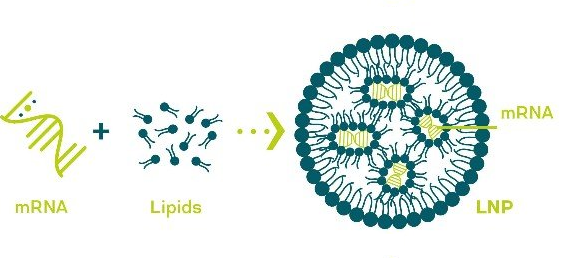
\includegraphics[width=0.7\textwidth]{image/cd_pl15_image1.png}
\end{center}
\figcaption{1}{Lipid nanoparticle (LNP) được cấu tạo bởi hai thành phần chính gồm mRNA và phospholipid}

Quy trình nghiên cứu và sản xuất vaccine mRNA được thực hiện qua hai giai đoạn chính sau đây:

\textbf{Giai đoạn 1 -- Nghiên cứu mầm bệnh và thiết kế gene:} mục đích tìm ra các protein có tính kháng nguyên (thường là các protein ở mặt ngoài mầm bệnh như protein màng, protein gai hoặc capsome), kháng nguyên này phải kích thích tạo kháng thể tiêu diệt mầm bệnh hiệu quả. Giải trình tự amino acid của protein, xác định gene mã hóa nên protein của mầm bệnh và cắt gene đó hoặc tổng hợp DNA nhân tạo. Dựa vào đoạn DNA thu nhận được để thiết kế gene.

\textbf{Giai đoạn 2 -- Sản xuất vaccine:}
\begin{itemize}[leftmargin=2em, itemsep=1pt, label=--]
\item Bước 1: Sử dụng vector plasmid để tạo DNA tái tổ hợp mang gene quy định kháng nguyên.
\item Bước 2: Chuyển plasmid vào vi khuẩn \textit{E. coli}. Phân lập dòng vi khuẩn nhận gene và nuôi trên quy mô công nghiệp nhằm tạo ra lượng plasmid lớn. Tinh chế, thu nhận plasmid.
\item Bước 3: Cắt mở vòng plasmid tạo DNA xoắn kép dạng thẳng.
\item Bước 4: Sử dụng hệ thống phiên mã nhân tạo để phiên mã tạo ra mRNA.
\item Bước 5: Lọc và tinh chế mRNA.
\item Bước 6: Kiểm tra chất lượng của mRNA.
\item Bước 7: Tạo hạt lipid nanoparticle (LNP) chứa mRNA.
\item Bước 8: Đóng gói thành phẩm.
\item Bước 9: Kiểm tra chất lượng và phân phối.
\end{itemize}

Tuy vaccine mRNA yêu cầu công nghệ cao, bảo quản khá phức tạp và chỉ có một vài loại được sản xuất nhưng nó đã thể hiện được một số ưu điểm và tiềm năng vượt trội so với các loại vaccine truyền thống như: có hiệu quả cao; an toàn, ít phản ứng phụ và không làm thay đổi DNA của tế bào; thời gian sản xuất ngắn và dễ nhân rộng quy mô sản xuất; có thể nhanh chóng tùy biến vaccine thông qua điều chỉnh mã di truyền trên mRNA; có tiềm năng tạo ra vaccine hiệu quả để phòng virus cúm, HIV,... phòng và điều trị ung thư. Các loại vaccine mRNA đã chứng minh hiệu quả trong việc đẩy lùi đại dịch COVID-19 như Spikevax (mRNA-1273) của công ti Moderna và Comirnaty (BNT162b2) của công ti Pfizer-BioNTech. Năm 2023, hai nhà khoa học Katalin Kariko và Drew Weissman được trao tặng giải Nobel Y Sinh cho những đóng góp của họ trong nghiên cứu vaccine mRNA.
\hfill\textbf{Nguồn: Thầy Đào Anh Phúc biên soạn}
\end{readingpassage}
\vspace{2pt}
% ── CÂU HỎI ──

% === Câu 1: Trắc nghiệm ===
\question[Trắc nghiệm]{Theo bài đọc, vaccine cung cấp cho cơ thể thành phần nào để kích thích tạo miễn dịch đặc hiệu và ghi nhớ miễn dịch?}
\par\vspace{4pt}
\noindent\hangindent=2.2em\hangafter=1\choiceitem{A}{Kháng thể đặc hiệu với mầm bệnh.}\par\vspace{4pt}
\noindent\hangindent=2.2em\hangafter=1\choiceitem{B}{Tế bào miễn dịch đã được ghi nhớ.}\par\vspace{4pt}
\noindent\hangindent=2.2em\hangafter=1\choiceitem{C}{Kháng nguyên của mầm bệnh.}\par\vspace{4pt}
\noindent\hangindent=2.2em\hangafter=1\choiceitem{D}{Kháng sinh tiêu diệt mầm bệnh.}\par\vspace{4pt}

% === Câu 2: Điền khuyết ===
\question[Điền khuyết]{Theo cách phân loại trong bài đọc, vaccine \dropbox[3cm] là loại vaccine chứa mầm bệnh còn sống nhưng đã được làm mất khả năng gây bệnh.\\[3pt]
\textit{(Điền từ/cụm từ (không quá 2 tiếng) hoặc số (làm tròn đến hàng đơn vị) vào chỗ trống.)}}
\vspace{2pt}

% === Câu 3: Ghép đôi ===
\question[Ghép đôi]{Ghép mỗi loại vaccine (Cột A) với đặc điểm thành phần tương ứng (Cột B).}

\vspace{6pt}
\setstretch{1.3}

\textit{Cột B:}
\vspace{-6pt}
\par\vspace{4pt}
\noindent\hangindent=2.2em\hangafter=1\choiceitem{A}{Chứa độc tố của vi khuẩn đã bị làm mất tính năng gây độc.}\par\vspace{4pt}
\noindent\hangindent=2.2em\hangafter=1\choiceitem{B}{Không chứa kháng nguyên mà chứa thông tin di truyền quy định kháng nguyên.}\par\vspace{4pt}
\noindent\hangindent=2.2em\hangafter=1\choiceitem{C}{Chứa mầm bệnh còn sống nhưng đã mất khả năng gây bệnh.}\par\vspace{4pt}
\noindent\hangindent=2.2em\hangafter=1\choiceitem{D}{Chứa mầm bệnh đã chết.}\par\vspace{4pt}
\noindent\hangindent=2.2em\hangafter=1\choiceitem{E}{Chứa kháng thể nhân tạo có sẵn để tiêu diệt trực tiếp mầm bệnh.}\par\vspace{4pt}
\vspace{6pt}
\renewcommand{\arraystretch}{1.6}
{\small\setstretch{1.0}
\begin{longtable}{|>{\raggedright\arraybackslash}m{0.55\textwidth}|>{\centering\arraybackslash}m{0.28\textwidth}|}
\hline
\rowcolor{primaryBlue!12}
\multicolumn{1}{|c|}{\cellcolor{primaryBlue!12}\textbf{Cột A}} & \cellcolor{primaryBlue!12}\textbf{Cột B} \\
\hline
\endfirsthead
\hline
\rowcolor{primaryBlue!12}
\multicolumn{1}{|c|}{\cellcolor{primaryBlue!12}\textbf{Cột A}} & \cellcolor{primaryBlue!12}\textbf{Cột B} \\
\hline
\endhead
1. Vaccine nhược độc & \dropbox[2.5cm] \\
\hline
2. Vaccine vô hoạt & \dropbox[2.5cm] \\
\hline
3. Vaccine giải độc tố & \dropbox[2.5cm] \\
\hline
4. Vaccine nucleic acid & \dropbox[2.5cm] \\
\hline
\end{longtable}
}
}

% === Câu 4: Kéo thả ===
\question[Kéo thả]{Kéo các cụm từ thích hợp vào chỗ trống để tóm tắt nguyên lí hoạt động của vaccine mRNA.
\vspace{-4pt}
\dragitems{
\centering
    \dragitem{kháng nguyên} \dragitem{kháng thể} \dragitem{LNP}\\[1pt]
    \dragitem{phospholipid} \dragitem{tế bào chất} \dragitem{ghi nhớ miễn dịch}
}
\setstretch{1.4}
Phân tử mRNA mang thông tin quy định (1)\,\dropbox[2.5cm] đặc trưng của mầm bệnh được đóng gói và giữ ổn định bên trong hạt (2)\,\dropbox[2cm]. Khi tiêm vào cơ thể, thành phần (3)\,\dropbox[2.5cm] giúp hạt này dung hợp với màng tế bào và giải phóng mRNA vào (4)\,\dropbox[2.5cm]. Nhờ đó, tế bào tổng hợp được protein kháng nguyên, hệ miễn dịch tạo kháng thể và (5)\,\dropbox[3cm] mầm bệnh.
}
\vspace{2pt}

% === Câu 5: Trắc nghiệm ===
\question[Trắc nghiệm]{Điểm đặc biệt của vaccine nucleic acid so với các loại vaccine truyền thống là gì?}
\par\vspace{4pt}
\noindent\hangindent=2.2em\hangafter=1\choiceitem{A}{Cần thử nghiệm trước khi sử dụng đại trà.}\par\vspace{4pt}
\noindent\hangindent=2.2em\hangafter=1\choiceitem{B}{Tạo miễn dịch đặc hiệu và ghi nhớ miễn dịch.}\par\vspace{4pt}
\noindent\hangindent=2.2em\hangafter=1\choiceitem{C}{Không mang sẵn thành phần có tính kháng nguyên.}\par\vspace{4pt}
\noindent\hangindent=2.2em\hangafter=1\choiceitem{D}{Được sử dụng bằng hình thức tiêm.}\par\vspace{4pt}

% === Câu 6: Trắc nghiệm ===
\question[Trắc nghiệm]{Phân tử mRNA trong vaccine mRNA có đặc điểm nào sau đây?}
\par\vspace{4pt}
\noindent\hangindent=2.2em\hangafter=1\choiceitem{A}{Mã hóa các phospholipid và glycolipid của mầm bệnh.}\par\vspace{4pt}
\noindent\hangindent=2.2em\hangafter=1\choiceitem{B}{Mã hóa một hoặc một vài protein có tính kháng nguyên của mầm bệnh.}\par\vspace{4pt}
\noindent\hangindent=2.2em\hangafter=1\choiceitem{C}{Mã hóa thành phần cấu tạo của tế bào bình thường của cơ thể.}\par\vspace{4pt}
\noindent\hangindent=2.2em\hangafter=1\choiceitem{D}{Mang toàn bộ thông tin di truyền quy định mọi cấu tạo của mầm bệnh.}\par\vspace{4pt}

% === Câu 7: Đúng/Sai ===
\question[Đúng/Sai]{Đánh giá tính đúng/sai của các phát biểu về cơ chế hoạt động của vaccine mRNA sau khi tiêm vào cơ thể:}

\truefalsehead
\truefalseitem{a) Tế bào sử dụng mRNA của vaccine làm khuôn để tổng hợp các protein có tính kháng nguyên của mầm bệnh.}
\truefalseitem{b) Tế bào nhận biết protein kháng nguyên là protein lạ và đưa chúng ra phía ngoài màng nhân.}
\truefalseitem{c) Hệ miễn dịch đặc hiệu nhận biết kháng nguyên, tạo kháng thể và ghi nhớ mầm bệnh.}
\truefalseitem{d) mRNA của vaccine được phiên mã ngược tạo DNA để gắn với DNA của tế bào.}
\truefalseend
% === Câu 8: Trắc nghiệm ===
\question[Trắc nghiệm]{Phát biểu nào sau đây là SAI khi nói về lipid nanoparticle (LNP)?}
\par\vspace{4pt}
\noindent\hangindent=2.2em\hangafter=1\choiceitem{A}{LNP gồm hai thành phần chính là phospholipid và mRNA.}\par\vspace{4pt}
\noindent\hangindent=2.2em\hangafter=1\choiceitem{B}{LNP giúp giữ ổn định cấu trúc của phân tử mRNA.}\par\vspace{4pt}
\noindent\hangindent=2.2em\hangafter=1\choiceitem{C}{LNP giúp mRNA dung hợp với màng tế bào.}\par\vspace{4pt}
\noindent\hangindent=2.2em\hangafter=1\choiceitem{D}{LNP giúp đưa mRNA vào trong tế bào chất.}\par\vspace{4pt}

% === Câu 9: Điền khuyết ===
\question[Điền khuyết]{Vaccine mRNA có hiệu quả cao trong phòng virus vì quá trình tạo ra kháng nguyên từ mRNA diễn ra tương tự như giai đoạn \dropbox[3cm] của virus trong tế bào chủ.\\[3pt]
\textit{(Điền từ/cụm từ (không quá 2 tiếng) hoặc số (làm tròn đến hàng đơn vị) vào chỗ trống.)}}
\vspace{2pt}

% === Câu 10: Đúng/Sai ===
\question[Đúng/Sai]{Đánh giá tính đúng/sai của các phát biểu về quy trình sản xuất vaccine mRNA:}

\truefalsehead
\truefalseitem{a) \textit{E. coli} được chọn ở bước 2 vì vi khuẩn này có khả năng phiên mã trực tiếp tạo ra mRNA vaccine.}
\truefalseitem{b) Nếu bỏ qua bước 5 (lọc, tinh chế mRNA), sản phẩm cuối cùng vẫn đảm bảo chất lượng vì bước 6 đã có khâu kiểm tra.}
\truefalseitem{c) DNA tái tổ hợp được tạo ra nhờ vector plasmid mang gene quy định protein kháng nguyên.}
\truefalseitem{d) Kháng nguyên được chọn để thiết kế vaccine thường là protein nằm ở mặt ngoài của mầm bệnh.}
\truefalseend
% === Câu 11: Ghép đôi ===
\question[Ghép đôi]{Nối mỗi bước/giai đoạn trong quy trình sản xuất (Cột A) với mục đích tương ứng (Cột B).}

\vspace{6pt}
\setstretch{1.3}

\textit{Cột B:}
\vspace{-6pt}
\par\vspace{4pt}
\noindent\hangindent=2.2em\hangafter=1\choiceitem{A}{Bảo vệ, giữ ổn định phân tử mRNA và giúp đưa mRNA vào tế bào chất.}\par\vspace{4pt}
\noindent\hangindent=2.2em\hangafter=1\choiceitem{B}{Xác định và thiết kế gene mã hóa protein kháng nguyên của mầm bệnh.}\par\vspace{4pt}
\noindent\hangindent=2.2em\hangafter=1\choiceitem{C}{Nhân rộng plasmid trên quy mô công nghiệp nhờ hoạt động của vi khuẩn.}\par\vspace{4pt}
\noindent\hangindent=2.2em\hangafter=1\choiceitem{D}{Tạo DNA xoắn kép dạng thẳng để chuẩn bị khuôn cho quá trình phiên mã.}\par\vspace{4pt}
\noindent\hangindent=2.2em\hangafter=1\choiceitem{E}{Tổng hợp trực tiếp protein kháng nguyên bằng hệ thống dịch mã nhân tạo.}\par\vspace{4pt}
\vspace{6pt}
\renewcommand{\arraystretch}{1.6}
{\small\setstretch{1.0}
\begin{longtable}{|>{\raggedright\arraybackslash}m{0.55\textwidth}|>{\centering\arraybackslash}m{0.28\textwidth}|}
\hline
\rowcolor{primaryBlue!12}
\multicolumn{1}{|c|}{\cellcolor{primaryBlue!12}\textbf{Cột A}} & \cellcolor{primaryBlue!12}\textbf{Cột B} \\
\hline
\endfirsthead
\hline
\rowcolor{primaryBlue!12}
\multicolumn{1}{|c|}{\cellcolor{primaryBlue!12}\textbf{Cột A}} & \cellcolor{primaryBlue!12}\textbf{Cột B} \\
\hline
\endhead
1. Bước 2: Chuyển plasmid tái tổ hợp vào \textit{E. coli} & \dropbox[2.5cm] \\
\hline
2. Bước 3: Cắt mở vòng plasmid & \dropbox[2.5cm] \\
\hline
3. Bước 7: Tạo các hạt lipid nanoparticle (LNP) & \dropbox[2.5cm] \\
\hline
4. Giai đoạn 1: Thiết kế gene & \dropbox[2.5cm] \\
\hline
\end{longtable}
}

% === Câu 12: Đúng/Sai ===
\question[Đúng/Sai]{Đánh giá tính đúng/sai khi so sánh vaccine mRNA với các thế hệ vaccine truyền thống:}

\truefalsehead
\truefalseitem{a) Vaccine nhược độc chứa mầm bệnh còn sống nên tiềm ẩn rủi ro an toàn cao hơn vaccine vô hoạt.}
\truefalseitem{b) Vaccine mRNA làm thay đổi DNA của tế bào người được tiêm nên hiệu quả ghi nhớ miễn dịch kéo dài.}
\truefalseitem{c) Vì vaccine nucleic acid không chứa sẵn kháng nguyên, cơ thể người tiêm phải tự tổng hợp kháng nguyên từ thông tin di truyền được cung cấp.}
\truefalseitem{d) Chỉ cần tăng liều tiêm vaccine mRNA là có thể bảo quản vaccine ở nhiệt độ thường trong thời gian không hạn chế.}
\truefalseend
% === Câu 13: Điền khuyết ===
\question[Điền khuyết]{Giả sử xuất hiện một chủng virus mới gây bệnh ở người và các nhà khoa học muốn thiết kế vaccine mRNA.\\[3pt]
\textit{(Điền từ/cụm từ (không quá 2 tiếng) hoặc số (làm tròn đến hàng đơn vị) vào chỗ trống.)}}
\vspace{2pt}
\setstretch{1.4}
Các nhà khoa học cần ưu tiên chọn những protein nằm ở (1)\,\dropbox[3cm] của mầm bệnh làm kháng nguyên mục tiêu, vì đây là vị trí mà (2)\,\dropbox[3cm] do hệ miễn dịch tạo ra dễ dàng tiếp cận để tiêu diệt mầm bệnh. Sau khi giải trình tự amino acid của protein đó, họ xác định và thiết kế (3)\,\dropbox[3cm] mã hóa protein này rồi đưa vào quy trình sản xuất. Nếu sau này virus đột biến làm thay đổi protein bề mặt, việc tùy biến một vaccine mRNA mới chủ yếu chỉ cần điều chỉnh (4)\,\dropbox[4cm], nhờ đó rút ngắn đáng kể thời gian phát triển vaccine so với công nghệ truyền thống.


\newpage
\begin{center}
\begin{tikzpicture}
    \node[fill=primaryBlue, rounded corners=10pt,
          inner xsep=25pt, inner ysep=14pt,
          drop shadow={shadow xshift=2pt, shadow yshift=-2pt, opacity=0.3},
          text width=14cm, align=center]
    {%
        \color{white}\fontsize{22}{28}\selectfont\bfseries
\phantomsection\label{b2_chuyende3}
        Chuyên đề 3:\\Phanh ABS + Phanh tái sinh%
    };
\end{tikzpicture}
\end{center}

\vspace{-8pt}

% ============================================================
% CHỦ ĐỀ 1: SỰ CẢI TIẾN TRONG HỆ THỐNG PHANH
% ============================================================
\setcounter{qcounter}{0}

\phantomsection\label{b2_cd3_1}
\begin{topicbox}{\large CHỦ ĐỀ 1: SỰ CẢI TIẾN TRONG HỆ THỐNG PHANH}
\vspace{8pt}
\textit{Đọc đoạn văn sau và trả lời các câu hỏi.}
\vspace{6pt}
\end{topicbox}

\begin{readingpassage}[]
\setstretch{1.3}

Khi tham gia giao thông, phản xạ tự nhiên của người lái khi cần dừng gấp là đạp phanh hết cỡ cho bánh ngừng quay hoàn toàn. Tuy nhiên, xe bị khóa cứng bánh vừa có quãng đường dừng dài hơn, vừa mất khả năng chuyển hướng tránh chướng ngại. Lực phanh lớn hơn không đồng nghĩa với an toàn hơn. Nguyên nhân nằm ở cơ chế phanh truyền thống hoạt động theo nguyên lý đơn giản: khi đạp phanh, má phanh ép vào đĩa hoặc tang trống để giảm tốc độ quay của bánh. Nếu đạp thật mạnh, bánh có thể ngừng quay hẳn, gọi là ``khóa bánh''. Tưởng chừng bánh dừng quay sẽ giúp xe dừng nhanh nhất, nhưng thực tế ngược lại.

Khi bánh còn lăn, lốp duy trì ma sát tĩnh với mặt đường và đáp ứng hướng lái. Khi bánh khóa cứng, lốp không còn lăn mà trượt trên mặt đường. Ma sát trượt nhỏ hơn ma sát lăn, nên bánh trượt bám đường kém hơn đáng kể so với bánh lăn, khiến xe cần quãng đường dài hơn để dừng. Tệ hơn, bánh đang trượt thì mất khả năng đáp ứng tín hiệu lái: dù có đánh lái, xe vẫn lao thẳng về phía trước. Kết quả là xe khóa bánh trượt thẳng và va vào chướng ngại vật.

\begin{center}
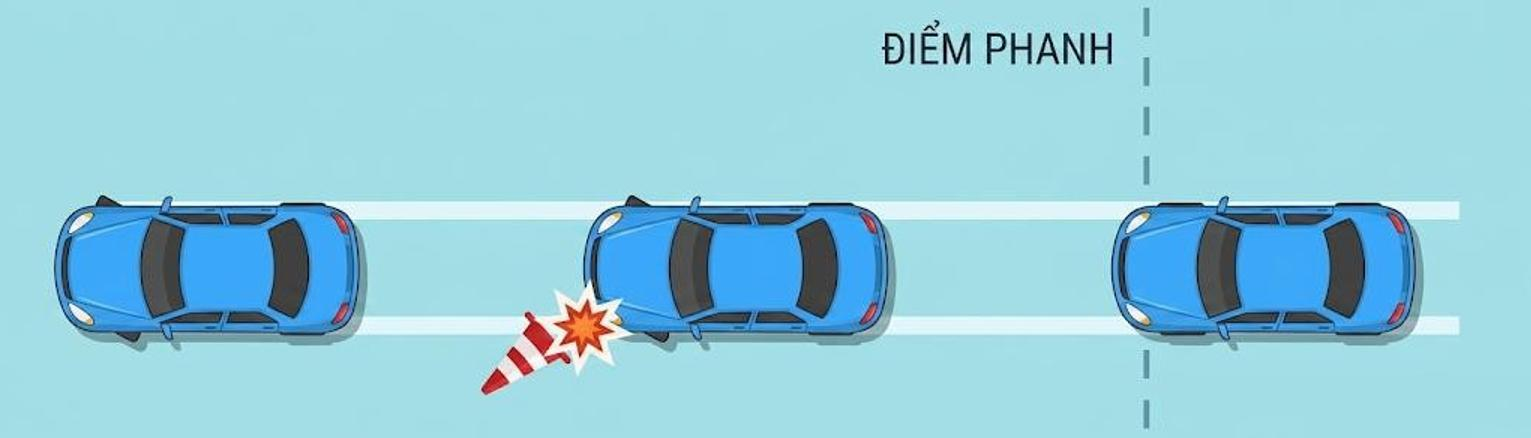
\includegraphics[width=0.7\textwidth]{image/abs_cd1_image2.png}
\end{center}
\figcaption{1}{Xe trượt đi khi phanh bị bó cứng.}

Những tài xế lành nghề từ lâu đã áp dụng kỹ thuật: thay vì giữ chặt phanh cho bánh khóa, họ nhấp--nhả phanh liên tục, lặp lại nhiều lần. Mỗi lần nhả, bánh kịp quay trở lại và bám đường; mỗi lần đạp, xe lại chậm thêm. Nhờ vậy bánh không bao giờ khóa cứng, xe vừa giảm tốc vừa còn lái được. Nhược điểm là con người nhấp khá chậm và trong tình huống khẩn cấp thì phản xạ không đủ nhanh.

Hệ thống chống bó cứng phanh (ABS) thực hiện chức năng ``nhấp--nhả'' ấy, nhưng tự động và nhanh hơn con người rất nhiều. Cảm biến gắn ở bánh liên tục theo dõi tốc độ quay; khi phát hiện bánh sắp khóa, hệ thống lập tức nhả phanh một chút cho bánh quay lại rồi ép phanh tiếp, lặp đi lặp lại hàng chục lần mỗi giây. Bánh xe nhờ đó luôn ở ngưỡng ``gần khóa mà chưa khóa'': vừa bám tốt để dừng ngắn, vừa còn lăn để đánh lái.

\begin{center}
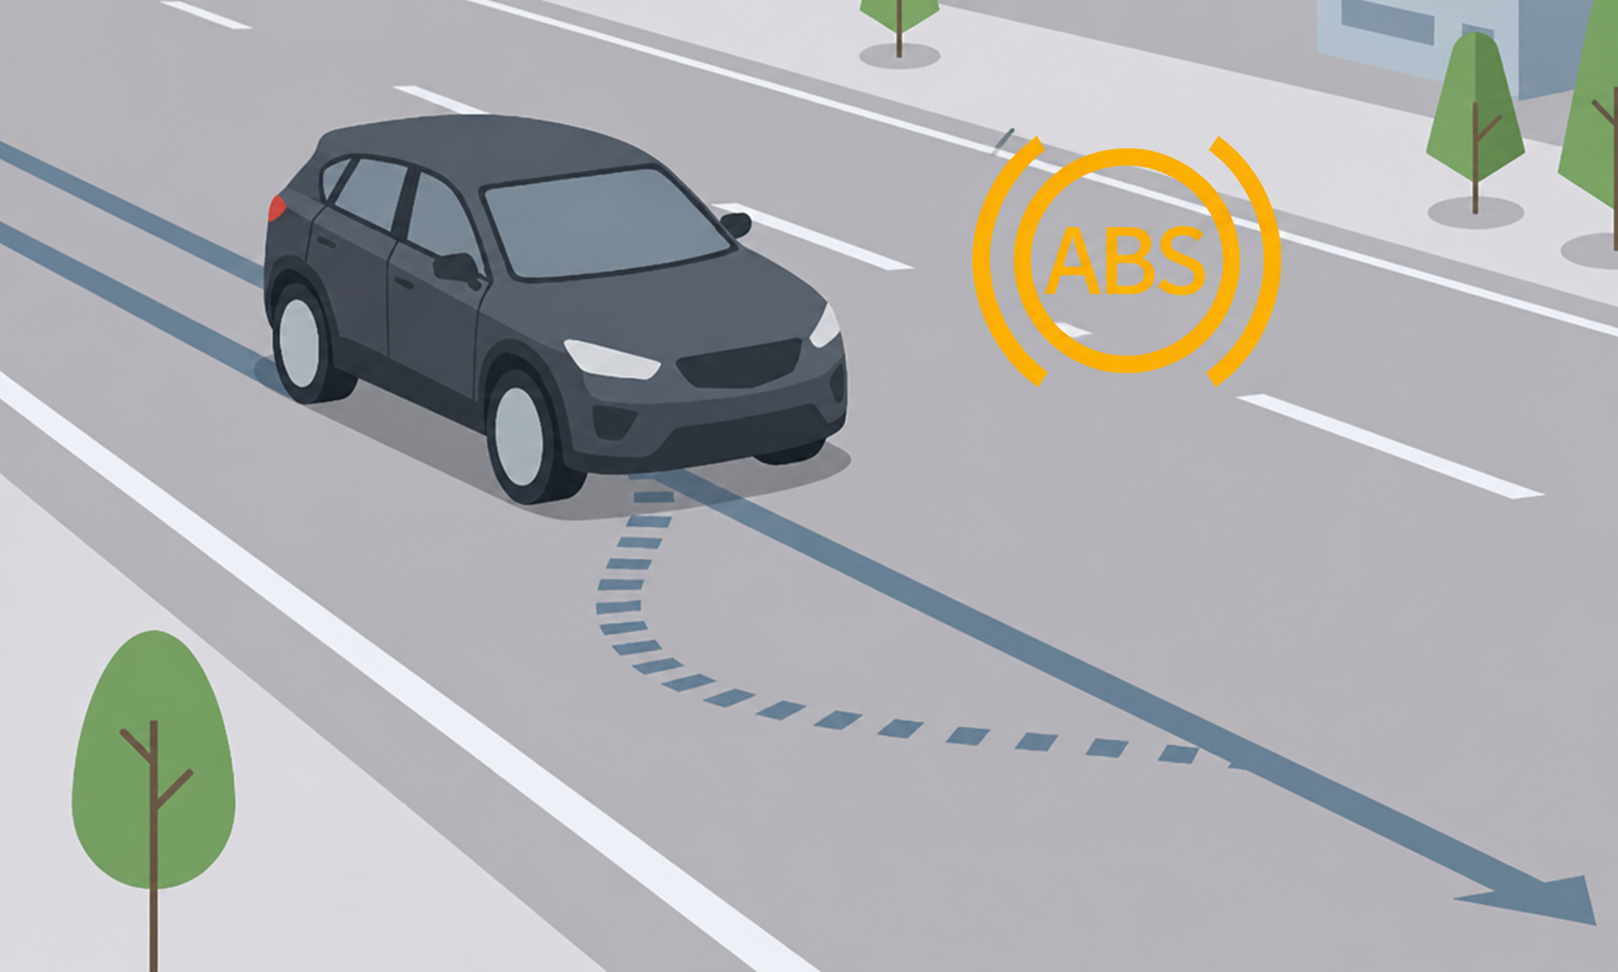
\includegraphics[width=0.55\textwidth]{image/abs_cd1_image3.png}
\end{center}
\figcaption{2}{Phanh ABS giúp xe khi phanh gấp.}

Nói cách khác, ABS không phanh mạnh hơn mà phanh khôn hơn, tức giữ bánh ngay ở mép giới hạn thay vì để bánh khóa cứng. Và để làm được điều đó, ABS phải liên tục đo tốc độ quay của từng bánh; cảm biến này còn được sử dụng cho nhiều chức năng khác.

\tablecaption{1}{So sánh ba cách phanh.}
\begin{center}
\renewcommand{\arraystretch}{1.3}
{\small
\setstretch{1.0}%
\begin{tabular}{|>{\raggedright\arraybackslash}m{3.5cm}|>{\centering\arraybackslash}m{3cm}|>{\centering\arraybackslash}m{3cm}|>{\centering\arraybackslash}m{3.5cm}|}
\hline
\rowcolor{primaryBlue!12}
\textbf{Tiêu chí} & \textbf{Phanh giữ chặt (khóa bánh)} & \textbf{Nhấp--nhả bằng tay} & \textbf{ABS} \\
\hline
Trạng thái bánh & Khóa cứng, trượt lê & Lúc lăn lúc khóa & Luôn gần ngưỡng, vẫn lăn \\
\hline
Giữ được lái? & Không & Một phần & Có \\
\hline
Quãng đường dừng & Dài nhất & Trung bình & Ngắn nhất \\
\hline
Số lần nhấp--nhả mỗi giây & 0 & Khoảng 1--3 (người) & Khoảng 15 (tự động) \\
\hline
\end{tabular}
}
\end{center}

\hfill\textbf{Nguồn: Nguyễn Nghĩa Đô biên soạn}
\end{readingpassage}

% --- CĐ 1: Câu hỏi ---

\question[Trắc nghiệm]{Dựa vào Hình 1, điều gì xảy ra với chiếc xe bị khóa bánh?}
\par\vspace{4pt}
\noindent\hangindent=2.2em\hangafter=1\choiceitem{A}{Xe từ từ giảm tốc độ và dừng lại an toàn.}\par\vspace{4pt}
\noindent\hangindent=2.2em\hangafter=1\choiceitem{B}{Xe trượt thẳng và đâm vào chướng ngại.}\par\vspace{4pt}
\noindent\hangindent=2.2em\hangafter=1\choiceitem{C}{Xe có thể đánh lái né được vật cản phía trước.}\par\vspace{4pt}
\noindent\hangindent=2.2em\hangafter=1\choiceitem{D}{Bánh xe tiếp tục lăn và bám sát mặt đường.}\par\vspace{4pt}

\question[Trắc nghiệm]{Khi nói ABS giữ cho bánh xe ``vẫn còn lăn'' trong lúc phanh gấp, điều đó nghĩa là gì?}
\par\vspace{4pt}
\noindent\hangindent=2.2em\hangafter=1\choiceitem{A}{Bánh vẫn đang được phanh nhưng chưa bị khóa cứng.}\par\vspace{4pt}
\noindent\hangindent=2.2em\hangafter=1\choiceitem{B}{Xe đã ngừng phanh hoàn toàn để bánh lăn tự do.}\par\vspace{4pt}
\noindent\hangindent=2.2em\hangafter=1\choiceitem{C}{Bánh bị khóa cứng nhưng quay chậm lại từ từ.}\par\vspace{4pt}
\noindent\hangindent=2.2em\hangafter=1\choiceitem{D}{Má phanh đã nhả hẳn khỏi bánh để tránh mài mòn.}\par\vspace{4pt}

\question[Trắc nghiệm]{Một tài xế báo: ``Tôi đã đạp phanh kịch sàn và đánh vô lăng hết cỡ nhưng xe không rẽ mà đâm thẳng vào cột điện''. Chẩn đoán nào đúng nhất?}
\par\vspace{4pt}
\noindent\hangindent=2.2em\hangafter=1\choiceitem{A}{Do ABS can thiệp quá mạnh làm hỏng vô lăng.}\par\vspace{4pt}
\noindent\hangindent=2.2em\hangafter=1\choiceitem{B}{Do má phanh kẹp không đủ mạnh nên xe không thể dừng.}\par\vspace{4pt}
\noindent\hangindent=2.2em\hangafter=1\choiceitem{C}{Do bánh xe khóa cứng chuyển sang trượt lê, làm mất khả năng lái.}\par\vspace{4pt}
\noindent\hangindent=2.2em\hangafter=1\choiceitem{D}{Do bánh xe còn lăn bám mặt đường quá tốt nên không thể rẽ.}\par\vspace{4pt}

\question[Đúng/Sai]{Các nhận định sau về cơ chế phanh truyền thống đúng hay sai?}

\vspace{6pt}
\renewcommand{\arraystretch}{1.4}
{\small\setstretch{1.0}
\begin{longtable}{|>{\raggedright\arraybackslash}m{0.72\textwidth}|>{\centering\arraybackslash}m{0.08\textwidth}|>{\centering\arraybackslash}m{0.08\textwidth}|}
\hline
\rowcolor{primaryBlue!12}
\textbf{Nội dung} & \textbf{Đúng} & \textbf{Sai} \\
\hline
\endfirsthead
\hline
\rowcolor{primaryBlue!12}
\textbf{Nội dung} & \textbf{Đúng} & \textbf{Sai} \\
\hline
\endhead
a) Đạp phanh càng mạnh làm khóa cứng bánh sẽ giúp xe dừng nhanh nhất. & \tfcircle & \tfcircle \\
\hline
b) Bánh trượt lê bám đường kém hơn hẳn bánh còn đang lăn. & \tfcircle & \tfcircle \\
\hline
c) ``Khóa bánh'' xảy ra khi má phanh không ép chặt vào bánh. & \tfcircle & \tfcircle \\
\hline
d) Khi bánh đang trượt, đánh vô lăng không đổi được hướng. & \tfcircle & \tfcircle \\
\hline
\end{longtable}
}

\question[Đúng/Sai]{Hệ thống phân phối lực phanh CBS phân phối lực phanh đều giữa bánh trước và bánh sau khi người lái bóp phanh. CBS không trang bị cảm biến tốc độ bánh và không có cơ chế tự nhả phanh.\\[3pt]
Dựa vào ngữ liệu và thông tin trên, đánh giá các mệnh đề:}

\vspace{6pt}
\renewcommand{\arraystretch}{1.4}
{\small\setstretch{1.0}
\begin{longtable}{|>{\raggedright\arraybackslash}m{0.72\textwidth}|>{\centering\arraybackslash}m{0.08\textwidth}|>{\centering\arraybackslash}m{0.08\textwidth}|}
\hline
\rowcolor{primaryBlue!12}
\textbf{Nội dung} & \textbf{Đúng} & \textbf{Sai} \\
\hline
\endfirsthead
\hline
\rowcolor{primaryBlue!12}
\textbf{Nội dung} & \textbf{Đúng} & \textbf{Sai} \\
\hline
\endhead
a) CBS không thể phát hiện bánh xe sắp bị khóa. & \tfcircle & \tfcircle \\
\hline
b) CBS giúp bánh xe không bao giờ bị khóa dù đạp phanh hết lực. & \tfcircle & \tfcircle \\
\hline
c) Ngay cả khi CBS phân phối đều, lực tổng quá lớn vẫn có thể khóa bánh. & \tfcircle & \tfcircle \\
\hline
d) Cả CBS lẫn ABS đều tự nhả phanh khi bánh sắp khóa. & \tfcircle & \tfcircle \\
\hline
\end{longtable}
}

\question[Điền khuyết]{Dựa vào Bảng 1, so với giới hạn tối đa của con người, ABS nhấp--nhả mỗi giây nhanh gấp khoảng bao nhiêu lần?\\[3pt]
\textit{(Điền từ/cụm từ (không quá 2 tiếng) hoặc số (làm tròn đến hàng đơn vị) vào chỗ trống.)}}
\vspace{2pt}
\setstretch{1.4}
Dựa vào Bảng 1, so với giới hạn tối đa của con người, ABS nhấp--nhả mỗi giây nhanh gấp khoảng (1)\,\dropbox[2cm] lần. Nhờ giữ bánh ở ngưỡng ``gần khóa mà chưa khóa'', bánh vẫn còn (2)\,\dropbox[2cm], tạo độ bám để đánh lái. Ngược lại, xe không có ABS lao thẳng vào chướng ngại dù đã bẻ lái là do bánh không còn quay mà chuyển sang trạng thái (3)\,\dropbox[2cm] trên đường.

\question[Ghép đôi]{Ghép mỗi trạng thái ở Cột A với hệ quả về lực bám ở Cột B.}

\vspace{6pt}
\setstretch{1.3}

\textit{Cột B:}
\vspace{-6pt}
\par\vspace{4pt}
\noindent\hangindent=2.2em\hangafter=1\choiceitem{A}{Tuột, bám kém, kéo lê như vật nặng}\par\vspace{4pt}
\noindent\hangindent=2.2em\hangafter=1\choiceitem{B}{Bánh kịp quay lại và bám đường}\par\vspace{4pt}
\noindent\hangindent=2.2em\hangafter=1\choiceitem{C}{Xe tự động phanh mạnh nhất có thể}\par\vspace{4pt}
\noindent\hangindent=2.2em\hangafter=1\choiceitem{D}{Bám mặt đường, ăn theo vô lăng}\par\vspace{4pt}
\noindent\hangindent=2.2em\hangafter=1\choiceitem{E}{Không nghe vô lăng, lao thẳng}\par\vspace{4pt}

\vspace{6pt}

\renewcommand{\arraystretch}{1.6}
{\small\setstretch{1.0}
\begin{longtable}{|>{\raggedright\arraybackslash}m{0.55\textwidth}|>{\centering\arraybackslash}m{0.28\textwidth}|}
\hline
\rowcolor{primaryBlue!12}
\multicolumn{1}{|c|}{\cellcolor{primaryBlue!12}\textbf{Cột A}} & \cellcolor{primaryBlue!12}\textbf{Cột B} \\
\hline
\endfirsthead
\hline
\rowcolor{primaryBlue!12}
\multicolumn{1}{|c|}{\cellcolor{primaryBlue!12}\textbf{Cột A}} & \cellcolor{primaryBlue!12}\textbf{Cột B} \\
\hline
\endhead
1. Bánh còn lăn bình thường & \dropbox[2.5cm] \\
\hline
2. Bánh bị khóa cứng & \dropbox[2.5cm] \\
\hline
3. Mỗi lần nhả phanh (khi nhấp--nhả) & \dropbox[2.5cm] \\
\hline
4. Bánh đang trượt & \dropbox[2.5cm] \\
\hline
\end{longtable}
}

\question[Ghép đôi]{Ghép mỗi cách phanh ở Cột A với bộ hệ quả đi kèm ở Cột B.}

\vspace{6pt}
\setstretch{1.3}

\textit{Cột B:}
\vspace{-6pt}
\par\vspace{4pt}
\noindent\hangindent=2.2em\hangafter=1\choiceitem{A}{Bánh luôn gần ngưỡng, dừng ngắn nhất và vẫn đánh lái được}\par\vspace{4pt}
\noindent\hangindent=2.2em\hangafter=1\choiceitem{B}{Bánh lúc lăn lúc khóa, giữ lái một phần nhưng phản xạ người không kịp}\par\vspace{4pt}
\noindent\hangindent=2.2em\hangafter=1\choiceitem{C}{Bánh trượt lê, quãng đường dài nhất và mất khả năng đánh lái}\par\vspace{4pt}
\noindent\hangindent=2.2em\hangafter=1\choiceitem{D}{Bánh không phanh, lăn tự do nên không giảm được tốc độ}\par\vspace{4pt}

\vspace{6pt}

\renewcommand{\arraystretch}{1.6}
{\small\setstretch{1.0}
\begin{longtable}{|>{\raggedright\arraybackslash}m{0.55\textwidth}|>{\centering\arraybackslash}m{0.28\textwidth}|}
\hline
\rowcolor{primaryBlue!12}
\multicolumn{1}{|c|}{\cellcolor{primaryBlue!12}\textbf{Cột A}} & \cellcolor{primaryBlue!12}\textbf{Cột B} \\
\hline
\endfirsthead
\hline
\rowcolor{primaryBlue!12}
\multicolumn{1}{|c|}{\cellcolor{primaryBlue!12}\textbf{Cột A}} & \cellcolor{primaryBlue!12}\textbf{Cột B} \\
\hline
\endhead
1. Đạp giữ chặt cho khóa bánh & \dropbox[2.5cm] \\
\hline
2. Nhấp--nhả bằng tay & \dropbox[2.5cm] \\
\hline
3. Hệ thống ABS & \dropbox[2.5cm] \\
\hline
\end{longtable}
}

\question[Kéo thả]{Kéo các cụm từ trong kho vào chỗ trống cho phù hợp:}
\vspace{-4pt}
\dragitems{
\centering
    \dragitem{lực kẹp} \dragitem{cảm biến} \dragitem{khóa cứng}\\[1pt]
    \dragitem{đánh lái} \dragitem{nhả phanh} \dragitem{tốc độ quay}
}

\setstretch{1.4}
ABS dùng (1)\,\dropbox[2cm] để liên tục theo dõi (2)\,\dropbox[2cm] của từng bánh. Khi phát hiện bánh sắp khóa, hệ thống lập tức (3)\,\dropbox[2cm] một chút để bánh kịp lăn trở lại. Nhờ vậy bánh tránh bị (4)\,\dropbox[2cm] hoàn toàn và xe vẫn đổi hướng được.

\question[Kéo thả]{So sánh hiệu quả ba cách phanh, kéo các cụm từ trong kho vào chỗ trống cho phù hợp:}
\vspace{-4pt}
\dragitems{
\centering
    \dragitem{trung bình} \dragitem{lực ma sát} \dragitem{khóa bánh}\\[1pt]
    \dragitem{lành nghề} \dragitem{gần ngưỡng} \dragitem{ngắn nhất}
}

\setstretch{1.4}
So với cách phanh giữ chặt có quãng đường dừng dài nhất, kỹ thuật nhấp--nhả của tài xế (1)\,\dropbox[2cm] giúp quãng đường đạt mức (2)\,\dropbox[2cm]. ABS tối ưu hơn hẳn vì luôn giữ bánh ở trạng thái (3)\,\dropbox[2cm], mang lại quãng đường dừng (4)\,\dropbox[2.5cm].

% ============================================================
% CHỦ ĐỀ 2: CẤU TRÚC PHANH ABS
% ============================================================
\newpage
\setcounter{qcounter}{0}

\phantomsection\label{b2_cd3_2}
\begin{topicbox}{\large CHỦ ĐỀ 2: CẤU TRÚC PHANH ABS}
\vspace{8pt}
\textit{Đọc đoạn văn sau và trả lời các câu hỏi.}
\vspace{6pt}
\end{topicbox}

\begin{readingpassage}[]
\setstretch{1.3}

Khi đèn ``ABS'' trên bảng đồng hồ bật sáng liên tục, xe vẫn phanh được, nhưng chức năng chống bó cứng đã ngừng. Chỉ một linh kiện trục trặc có thể khiến toàn bộ hệ thống mất dữ liệu đầu vào. Phần dưới đây trình bày cấu trúc ABS và cơ chế nhận biết bánh sắp khóa.

ABS không phải một cụm độc lập, mà tích hợp vào hệ thống phanh sẵn có. Khi đạp phanh, lực chân được bầu trợ lực phanh khuếch đại, truyền vào xy-lanh chính để tạo áp suất dầu đẩy tới các bánh. ABS bổ sung ba thành phần chính: ở mỗi bánh một cảm biến tốc độ đặt sát một vành răng tạo xung (đĩa nhiều răng cưa quay cùng bánh); một bộ điều khiển điện tử (ECBM) làm ``bộ não''; và một cụm van điều biến nằm trên đường dầu để nhả/ép áp suất phanh.

\begin{center}
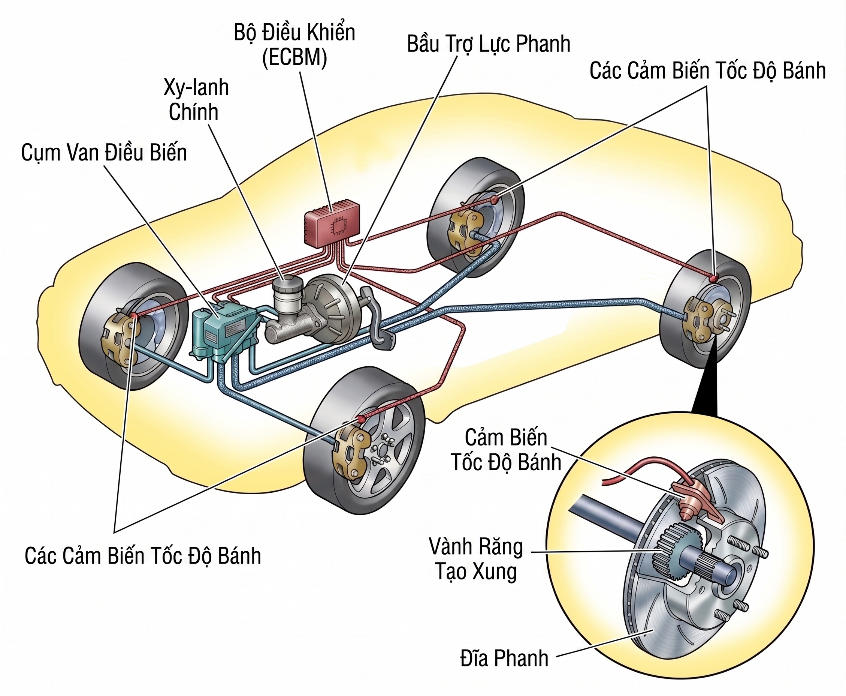
\includegraphics[width=0.55\textwidth]{image/abs_cd2_image2.png}
\end{center}
\figcaption{1}{Sơ đồ cấu tạo hệ thống phanh ABS.}

Nguyên lý hoạt động của cảm biến tốc độ: bánh quay thì vành răng quay theo, mỗi răng lướt qua đầu cảm biến sinh ra một ``xung''. Tần số xung (số xung mỗi giây) tỉ lệ thuận với tốc độ quay của bánh.

\tablecaption{1}{Bộ phận và chức năng.}
\begin{center}
\renewcommand{\arraystretch}{1.3}
{\small
\setstretch{1.0}%
\begin{tabular}{|>{\raggedright\arraybackslash}m{3.5cm}|>{\raggedright\arraybackslash}m{10cm}|}
\hline
\rowcolor{primaryBlue!12}
\textbf{Bộ phận} & \textbf{Chức năng} \\
\hline
Bầu trợ lực phanh & Khuếch đại lực đạp chân \\
\hline
Xy-lanh chính & Biến lực đạp thành áp suất dầu tới các bánh \\
\hline
Cảm biến và vành răng & Đếm răng đi qua để đo tốc độ quay từng bánh \\
\hline
Bộ điều khiển (ECBM) & ``Bộ não'': so sánh các bánh, phát hiện bánh sắp khóa, ra lệnh \\
\hline
Cụm van điều biến & Nhả hoặc ép áp suất dầu phanh tới từng bánh \\
\hline
\end{tabular}
}
\end{center}

\begin{center}
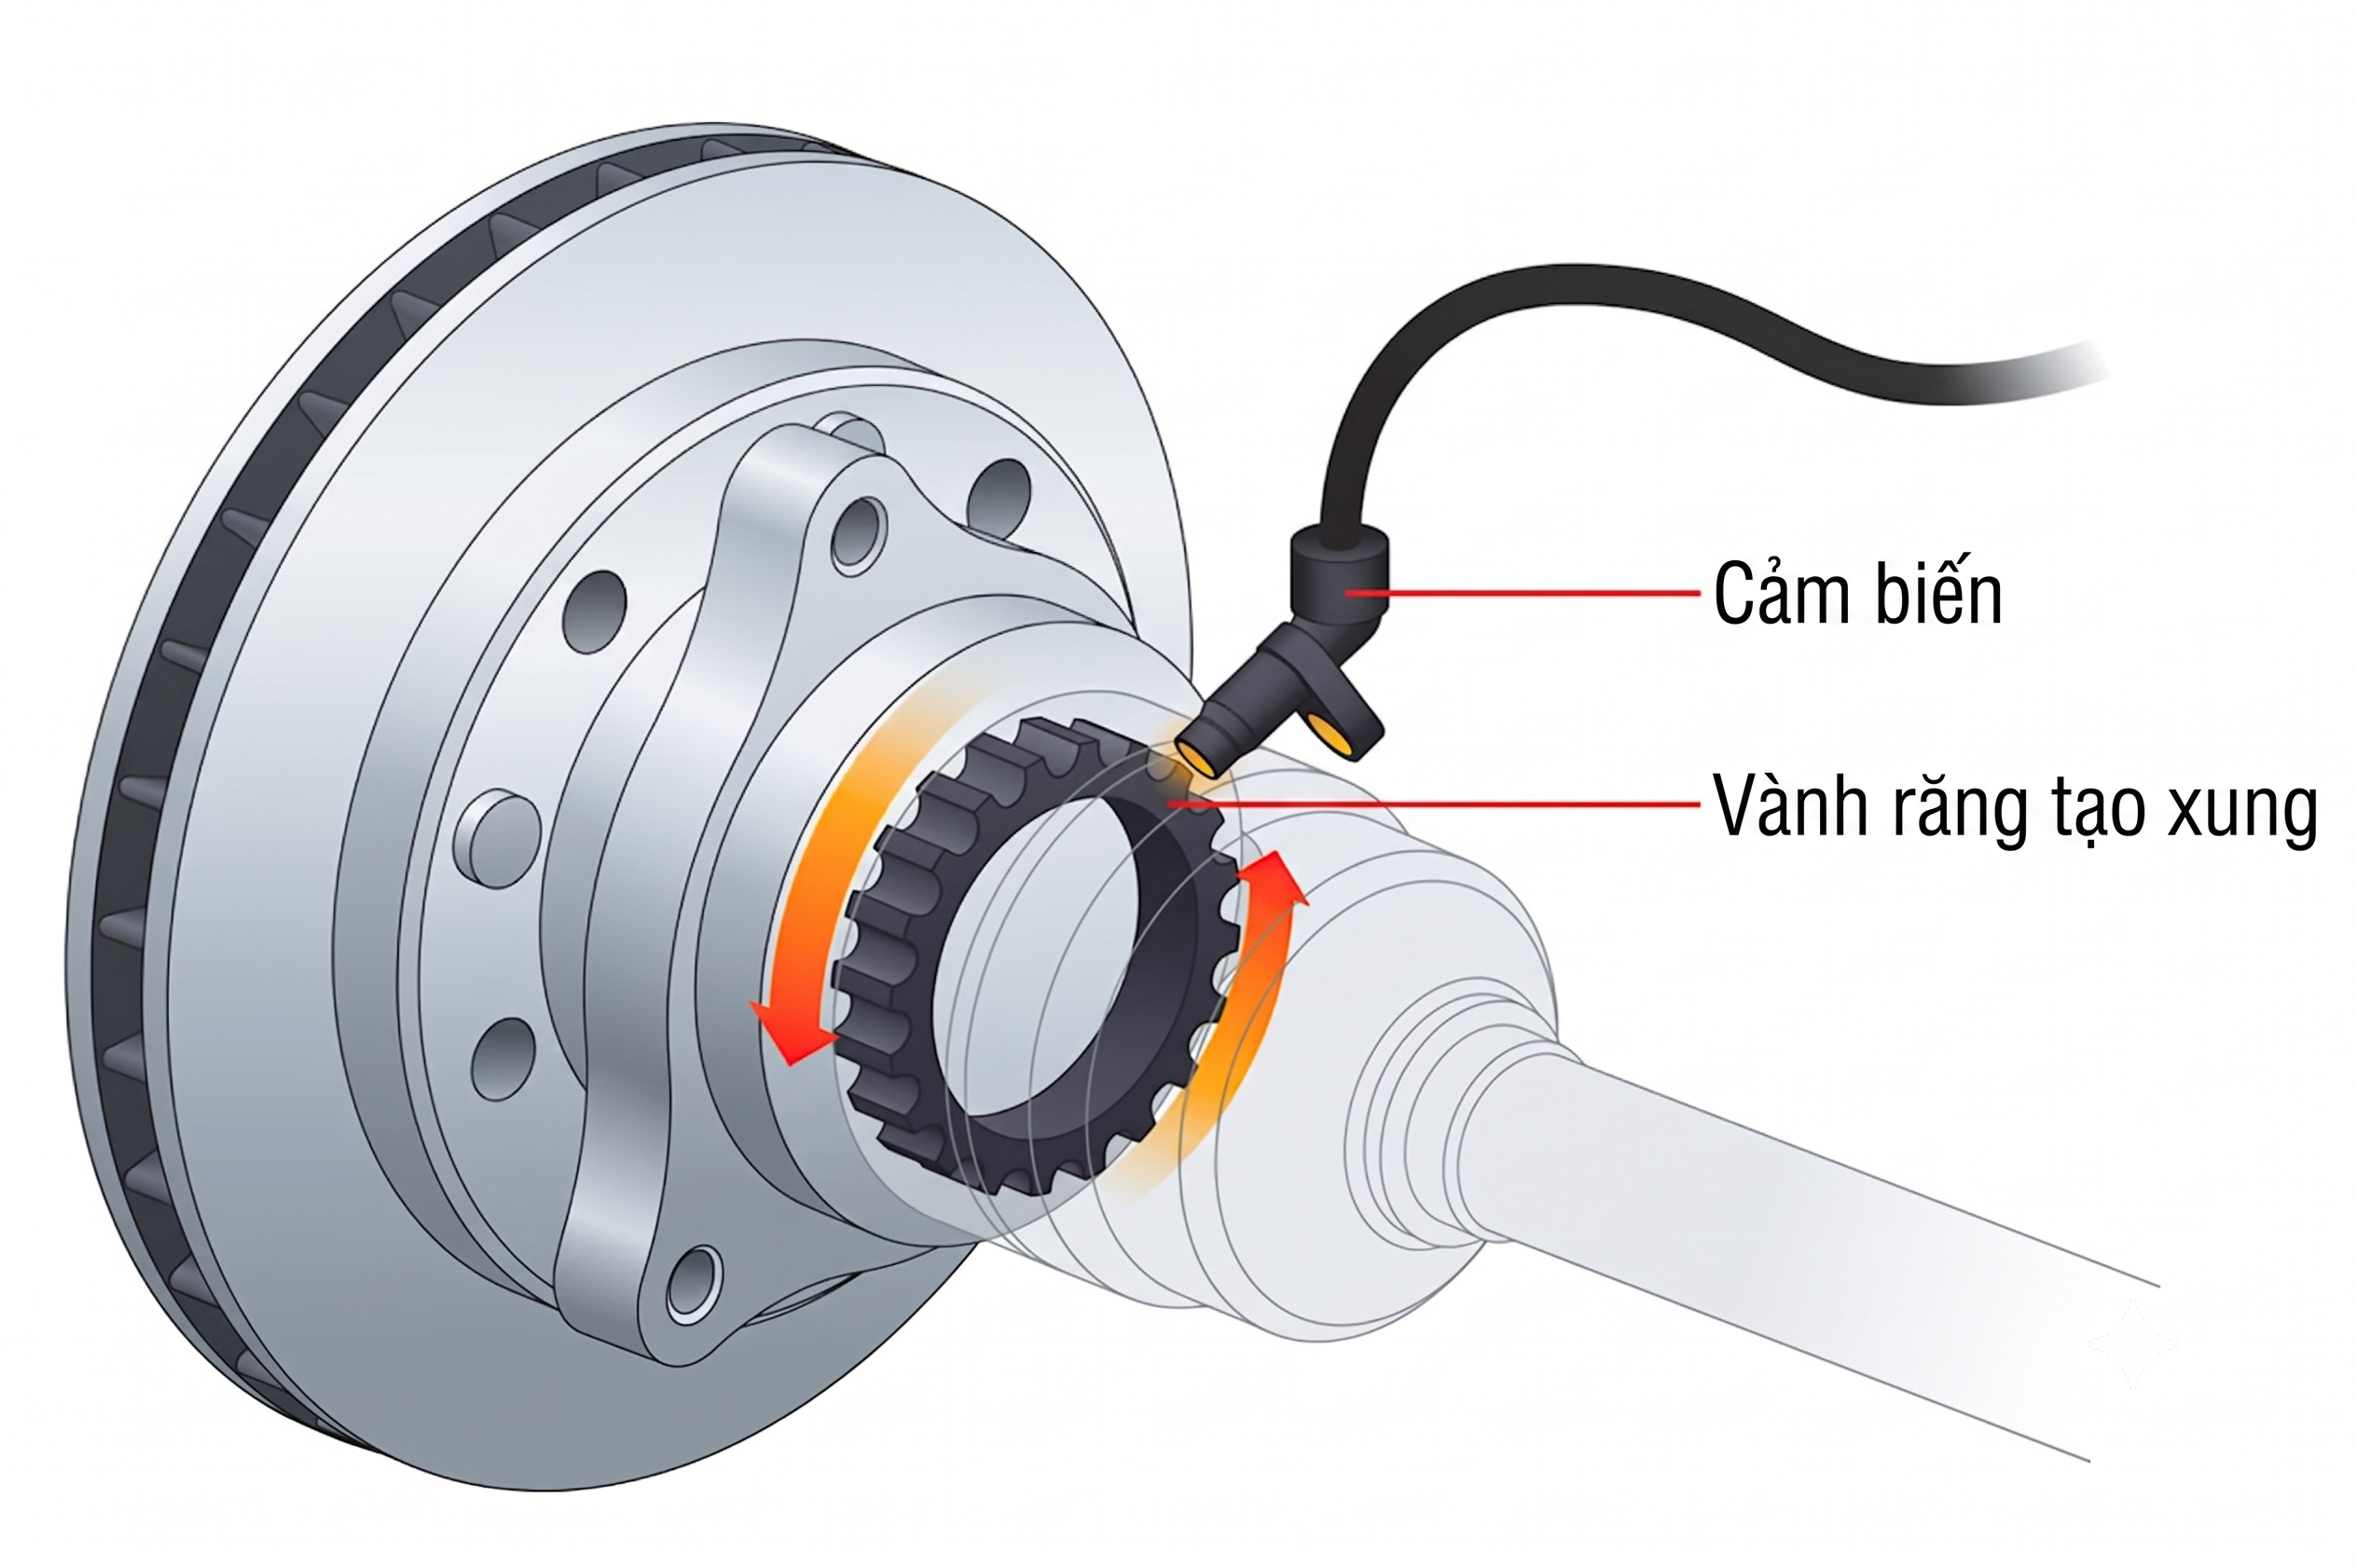
\includegraphics[width=0.45\textwidth]{image/abs_cd2_image3.png}
\end{center}
\figcaption{2}{Cảm biến ABS gắn sát vành răng tạo xung.}

Vành càng nhiều răng thì mỗi vòng tạo càng nhiều xung, nhờ đó phát hiện được cả những thay đổi nhỏ về tốc độ, tức độ phân giải phép đo cao hơn, nhất là lúc xe chạy chậm.

\tablecaption{2}{Số răng vành và độ mịn của phép đo.}
\begin{center}
\renewcommand{\arraystretch}{1.3}
{\small
\setstretch{1.0}%
\begin{tabular}{|>{\centering\arraybackslash}m{2.5cm}|>{\centering\arraybackslash}m{2cm}|>{\centering\arraybackslash}m{3cm}|>{\centering\arraybackslash}m{3cm}|}
\hline
\rowcolor{primaryBlue!12}
\textbf{Vành răng} & \textbf{Số răng} & \textbf{Số xung mỗi vòng} & \textbf{Độ mịn của phép đo} \\
\hline
Loại A & 48 & 48 & Thô hơn \\
\hline
Loại B & 96 & 96 & Mịn gấp đôi \\
\hline
\end{tabular}
}
\end{center}

Quy tắc: số xung mỗi giây bằng số răng nhân số vòng mỗi giây. Ví dụ bánh quay 10 vòng mỗi giây thì vành 48 răng cho 480 xung mỗi giây, vành 96 răng cho 960 xung mỗi giây.

Toàn bộ hệ thống hoạt động theo vòng điều khiển kín: cảm biến đo tốc độ, ECBM so sánh bốn bánh; phát hiện bánh nào giảm tốc đột ngột (sắp khóa) thì ra lệnh cho cụm van nhả bớt áp suất ở bánh đó rồi ép lại, lặp nhiều lần mỗi giây.

Vì mọi quyết định đều dựa vào cảm biến, chỉ cần một cảm biến bẩn, đứt dây hay gãy răng vành là ECBM mất ``mắt'' ở bánh đó. ECBM không thể điều khiển mù nên tắt ABS và bật đèn cảnh báo. Khi đó phanh thường vẫn hoạt động bình thường; vì vậy khi đèn ABS sáng, bước chẩn đoán đầu tiên là kiểm tra cảm biến và vành răng.

Đáng chú ý, cảm biến này không chỉ để chống khóa. Cùng dòng dữ liệu tốc độ quay ấy, hệ thống còn tính toán được bánh đang trượt nhiều hay ít, từ đó ước lượng đường trơn hay bám. Cảm biến tốc độ bánh vì thế là một ``cầu nối'' dùng chung cho nhiều hệ thống, không phải bộ phận rời.

\tablecaption{3}{Ảnh hưởng của khe hở cảm biến -- vành răng.}
\begin{center}
\renewcommand{\arraystretch}{1.3}
{\small
\setstretch{1.0}%
\begin{tabular}{|>{\centering\arraybackslash}m{2.5cm}|>{\centering\arraybackslash}m{3cm}|>{\centering\arraybackslash}m{3.5cm}|}
\hline
\rowcolor{primaryBlue!12}
\textbf{Khe hở (mm)} & \textbf{Biên độ xung (mV)} & \textbf{Hệ thống nhận tín hiệu} \\
\hline
0,3 & 900 & Ổn định \\
\hline
0,7 & 500 & Ổn định \\
\hline
1,1 & 200 & Chập chờn \\
\hline
1,5 & 80 & Mất tín hiệu \\
\hline
\end{tabular}
}
\end{center}

\hfill\textbf{Nguồn: Nguyễn Nghĩa Đô biên soạn}
\end{readingpassage}

% --- CĐ 2: Câu hỏi ---

\question[Trắc nghiệm]{Dựa vào Bảng 1, bộ phận nào đóng vai ``bộ não'', so sánh tốc độ các bánh và ra lệnh?}
\par\vspace{4pt}
\noindent\hangindent=2.2em\hangafter=1\choiceitem{A}{Cảm biến tốc độ.}\par\vspace{4pt}
\noindent\hangindent=2.2em\hangafter=1\choiceitem{B}{Cụm van điều biến.}\par\vspace{4pt}
\noindent\hangindent=2.2em\hangafter=1\choiceitem{C}{Bộ điều khiển (ECBM).}\par\vspace{4pt}
\noindent\hangindent=2.2em\hangafter=1\choiceitem{D}{Bầu trợ lực phanh.}\par\vspace{4pt}

\question[Trắc nghiệm]{Vì sao vành răng nhiều răng lại đặc biệt có lợi khi xe chạy chậm?}
\par\vspace{4pt}
\noindent\hangindent=2.2em\hangafter=1\choiceitem{A}{Vì chạy chậm bánh quay ít vòng, cần nhiều răng để vẫn tạo đủ xung đo chi tiết.}\par\vspace{4pt}
\noindent\hangindent=2.2em\hangafter=1\choiceitem{B}{Vì nhiều răng làm bánh xe quay nhanh hơn, bù cho tốc độ thấp.}\par\vspace{4pt}
\noindent\hangindent=2.2em\hangafter=1\choiceitem{C}{Vì nhiều răng giúp xy-lanh chính tạo áp suất phanh lớn hơn.}\par\vspace{4pt}
\noindent\hangindent=2.2em\hangafter=1\choiceitem{D}{Vì chạy chậm thì bộ điều khiển ngừng đếm xung để tiết kiệm điện.}\par\vspace{4pt}

\question[Trắc nghiệm]{Cảm biến tốc độ bắt được tốc độ bánh xe thông qua cơ chế nào?}
\par\vspace{4pt}
\noindent\hangindent=2.2em\hangafter=1\choiceitem{A}{Đo áp suất dầu trên đường ống phanh.}\par\vspace{4pt}
\noindent\hangindent=2.2em\hangafter=1\choiceitem{B}{Đo nhiệt độ sinh ra do ma sát tại đĩa phanh.}\par\vspace{4pt}
\noindent\hangindent=2.2em\hangafter=1\choiceitem{C}{Đếm số răng của vành răng lướt qua.}\par\vspace{4pt}
\noindent\hangindent=2.2em\hangafter=1\choiceitem{D}{Đo lực đạp trực tiếp từ chân tài xế.}\par\vspace{4pt}

\question[Trắc nghiệm]{Xe bị đứt dây tín hiệu ở cảm biến bánh trước bên trái, tài xế đạp phanh gấp trên đường trơn. Phản ứng của hệ thống là gì?}
\par\vspace{4pt}
\noindent\hangindent=2.2em\hangafter=1\choiceitem{A}{Xe mất phanh hoàn toàn vì ECBM tắt mọi hệ thống.}\par\vspace{4pt}
\noindent\hangindent=2.2em\hangafter=1\choiceitem{B}{Bơm hồi tự tạo áp suất mạnh hơn để bù đắp.}\par\vspace{4pt}
\noindent\hangindent=2.2em\hangafter=1\choiceitem{C}{Đèn ABS sáng, bánh trước bên trái vẫn có thể bị bó cứng.}\par\vspace{4pt}
\noindent\hangindent=2.2em\hangafter=1\choiceitem{D}{Cảm biến tự động đo bằng nhiệt độ để thay thế.}\par\vspace{4pt}

\question[Đúng/Sai]{Một kỹ thuật viên giữ tốc độ bánh không đổi, thay đổi khe hở giữa đầu cảm biến và vành răng, rồi đo biên độ xung thu được, kết quả ở Bảng 3.\\[3pt]
Dựa vào Bảng 3, các nhận định sau đúng hay sai?}

\vspace{6pt}
\renewcommand{\arraystretch}{1.4}
{\small\setstretch{1.0}
\begin{longtable}{|>{\raggedright\arraybackslash}m{0.72\textwidth}|>{\centering\arraybackslash}m{0.08\textwidth}|>{\centering\arraybackslash}m{0.08\textwidth}|}
\hline
\rowcolor{primaryBlue!12}
\textbf{Nội dung} & \textbf{Đúng} & \textbf{Sai} \\
\hline
\endfirsthead
\hline
\rowcolor{primaryBlue!12}
\textbf{Nội dung} & \textbf{Đúng} & \textbf{Sai} \\
\hline
\endhead
a) Khe hở càng lớn thì biên độ xung thu được càng giảm. & \tfcircle & \tfcircle \\
\hline
b) Ở khe hở 1,1\,mm, hệ thống vẫn nhận tín hiệu ổn định. & \tfcircle & \tfcircle \\
\hline
c) Khe hở lớn tới mức mất tín hiệu sẽ khiến ECBM báo lỗi giống như khi cảm biến bị bẩn hay đứt dây. & \tfcircle & \tfcircle \\
\hline
d) Muốn cảm biến chạy ổn định thì nên lắp khe hở càng lớn càng tốt. & \tfcircle & \tfcircle \\
\hline
\end{longtable}
}

\question[Đúng/Sai]{Xe vào xưởng: đèn ABS sáng liên tục, phanh vẫn bình thường; thợ thấy cảm biến bánh sau phải bị phủ kín bùn. Các nhận định sau đúng hay sai?}

\vspace{6pt}
\renewcommand{\arraystretch}{1.4}
{\small\setstretch{1.0}
\begin{longtable}{|>{\raggedright\arraybackslash}m{0.72\textwidth}|>{\centering\arraybackslash}m{0.08\textwidth}|>{\centering\arraybackslash}m{0.08\textwidth}|}
\hline
\rowcolor{primaryBlue!12}
\textbf{Nội dung} & \textbf{Đúng} & \textbf{Sai} \\
\hline
\endfirsthead
\hline
\rowcolor{primaryBlue!12}
\textbf{Nội dung} & \textbf{Đúng} & \textbf{Sai} \\
\hline
\endhead
a) Bùn đất đã làm thay đổi áp suất dầu trong đường ống phanh. & \tfcircle & \tfcircle \\
\hline
b) Lớp bùn cản cảm biến đếm răng, khiến ECBM mất dữ liệu tốc độ bánh này. & \tfcircle & \tfcircle \\
\hline
c) ECBM chủ động tắt chức năng ABS vì không dám ``điều khiển mù''. & \tfcircle & \tfcircle \\
\hline
d) Để khắc phục, chỉ cần thay mới cụm van điều biến. & \tfcircle & \tfcircle \\
\hline
\end{longtable}
}

\question[Điền khuyết]{Theo quy tắc ở Bảng 2, nếu ECBM nhận được 480 xung mỗi giây từ một bánh dùng vành Loại A (48 răng) thì bánh đang quay với tốc độ bao nhiêu?\\[3pt]
\textit{(Điền số (làm tròn đến hàng đơn vị) vào chỗ trống.)}}
\vspace{2pt}
\setstretch{1.4}
Bánh đang quay với tốc độ (1)\,\dropbox[2cm] vòng mỗi giây.

\question[Ghép đôi]{Ghép mỗi bộ phận ở Cột A với chức năng tương ứng ở Cột B.}

\vspace{6pt}
\setstretch{1.3}

\textit{Cột B:}
\vspace{-6pt}
\par\vspace{4pt}
\noindent\hangindent=2.2em\hangafter=1\choiceitem{A}{Đếm răng đi qua để đo tốc độ quay từng bánh}\par\vspace{4pt}
\noindent\hangindent=2.2em\hangafter=1\choiceitem{B}{Khuếch đại lực đạp chân}\par\vspace{4pt}
\noindent\hangindent=2.2em\hangafter=1\choiceitem{C}{Biến lực đạp thành áp suất dầu đẩy tới các bánh}\par\vspace{4pt}
\noindent\hangindent=2.2em\hangafter=1\choiceitem{D}{Nhả hoặc ép áp suất dầu tới từng bánh}\par\vspace{4pt}

\vspace{6pt}

\renewcommand{\arraystretch}{1.6}
{\small\setstretch{1.0}
\begin{longtable}{|>{\raggedright\arraybackslash}m{0.55\textwidth}|>{\centering\arraybackslash}m{0.28\textwidth}|}
\hline
\rowcolor{primaryBlue!12}
\multicolumn{1}{|c|}{\cellcolor{primaryBlue!12}\textbf{Cột A}} & \cellcolor{primaryBlue!12}\textbf{Cột B} \\
\hline
\endfirsthead
\hline
\rowcolor{primaryBlue!12}
\multicolumn{1}{|c|}{\cellcolor{primaryBlue!12}\textbf{Cột A}} & \cellcolor{primaryBlue!12}\textbf{Cột B} \\
\hline
\endhead
1. Xy-lanh chính & \dropbox[2.5cm] \\
\hline
2. Cụm van điều biến & \dropbox[2.5cm] \\
\hline
3. Cảm biến tốc độ & \dropbox[2.5cm] \\
\hline
\end{longtable}
}

\question[Ghép đôi]{Trong cụm van điều biến có một bơm hồi làm nhiệm vụ đẩy phần dầu vừa xả trở lại đường ống, giúp lần ép phanh tiếp theo vẫn có đủ lực. Ghép mỗi hiện tượng ở Cột A với kết luận đúng ở Cột B.}

\vspace{6pt}
\setstretch{1.3}

\textit{Cột B:}
\vspace{-6pt}
\par\vspace{4pt}
\noindent\hangindent=2.2em\hangafter=1\choiceitem{A}{Dầu vừa xả không được đẩy lại, thiếu lực cho lần ép phanh tiếp theo}\par\vspace{4pt}
\noindent\hangindent=2.2em\hangafter=1\choiceitem{B}{Số xung mỗi giây tăng gấp đôi, đo tốc độ mịn hơn}\par\vspace{4pt}
\noindent\hangindent=2.2em\hangafter=1\choiceitem{C}{Cảm biến hoặc vành răng bánh đó có thể bị lỗi}\par\vspace{4pt}
\noindent\hangindent=2.2em\hangafter=1\choiceitem{D}{Độ mịn phép đo tốc độ trở nên thô hơn}\par\vspace{4pt}
\noindent\hangindent=2.2em\hangafter=1\choiceitem{E}{Chỉ chức năng chống bó cứng mất, phanh thường còn nguyên}\par\vspace{4pt}
\noindent\hangindent=2.2em\hangafter=1\choiceitem{F}{Bơm hồi đang tạo thêm lực phanh}\par\vspace{4pt}

\vspace{6pt}

\renewcommand{\arraystretch}{1.6}
{\small\setstretch{1.0}
\begin{longtable}{|>{\raggedright\arraybackslash}m{0.55\textwidth}|>{\centering\arraybackslash}m{0.28\textwidth}|}
\hline
\rowcolor{primaryBlue!12}
\multicolumn{1}{|c|}{\cellcolor{primaryBlue!12}\textbf{Cột A}} & \cellcolor{primaryBlue!12}\textbf{Cột B} \\
\hline
\endfirsthead
\hline
\rowcolor{primaryBlue!12}
\multicolumn{1}{|c|}{\cellcolor{primaryBlue!12}\textbf{Cột A}} & \cellcolor{primaryBlue!12}\textbf{Cột B} \\
\hline
\endhead
1. Một bánh gửi về 0 xung khi xe đang chạy & \dropbox[2.5cm] \\
\hline
2. Thay vành 48 răng bằng vành 96 răng (cùng tốc độ) & \dropbox[2.5cm] \\
\hline
3. Bơm hồi trong cụm van bị hỏng & \dropbox[2.5cm] \\
\hline
4. Thay vành nhiều răng bằng vành ít răng & \dropbox[2.5cm] \\
\hline
5. Đèn ABS sáng nhưng đạp phanh xe vẫn dừng được & \dropbox[2.5cm] \\
\hline
\end{longtable}
}

\question[Kéo thả]{Kéo các cụm từ trong kho vào chỗ trống cho phù hợp:}
\vspace{-4pt}
\dragitems{
\centering
    \dragitem{đếm vòng} \dragitem{độ mịn} \dragitem{bị trượt}\\[1pt]
    \dragitem{nhiệt độ} \dragitem{cầu nối}
}

\setstretch{1.4}
Cảm biến tốc độ bánh không chỉ làm mỗi việc (1)\,\dropbox[2cm] để chống khóa phanh. Bằng cách phân tích cùng dòng dữ liệu, xe suy ra mức độ bánh (2)\,\dropbox[2cm] so với mặt đường. Điều này chứng tỏ cảm biến là một (3)\,\dropbox[2cm] cho nhiều hệ thống an toàn dùng chung.

% ============================================================
% CHỦ ĐỀ 3: CHU TRÌNH VAN ABS
% ============================================================
\newpage
\setcounter{qcounter}{0}

\phantomsection\label{b2_cd3_3}
\begin{topicbox}{\large CHỦ ĐỀ 3: CHU TRÌNH VAN ABS}
\vspace{8pt}
\textit{Đọc đoạn văn sau và trả lời các câu hỏi.}
\vspace{6pt}
\end{topicbox}

\begin{readingpassage}[]
\setstretch{1.3}

Hệ thống chống bó cứng phanh (ABS) không phanh chết một lần rồi thôi, mà ``nhả -- giữ -- ép'' áp suất phanh hàng chục lần mỗi giây để bánh không bị khóa. Tuy nhiên, ép quá mức sẽ khóa bánh, nhả quá nhiều sẽ mất lực phanh. Phần dưới đây trình bày cách cụm van xác định thời điểm và mức độ điều áp.

Khi điều khiển bàn đạp phanh, người lái thực hiện ba thao tác cơ bản: đạp mạnh thêm để tăng lực phanh, giữ nguyên chân để giữ lực phanh ở mức hiện tại, hay nhấc bớt chân để nhả bớt lực phanh. Mọi pha phanh đều là chuỗi ba động tác này nối tiếp nhau.

Về cơ chế truyền lực phanh: phanh ô tô là phanh thủy lực, lực đạp được truyền qua đường ống chứa dầu phanh thay vì cơ cấu cơ khí. Dầu là chất lỏng gần như không nén được, nên ép dầu ở đầu này thì áp lực lập tức truyền tới đầu kia, đẩy má phanh ép vào đĩa ở bánh. Nói cách khác, ``đường dầu'' chính là ống dẫn áp lực; điều tiết lực phanh thực chất là điều tiết áp suất dầu trong ống. Đây là chức năng của cụm van điều biến, thực hiện bằng cách đóng hoặc mở các đường dầu.

Tương ứng với ba thao tác phanh, van có ba trạng thái. Tăng áp: van mở đường cho áp suất từ xy-lanh chính và bơm dồn tới bánh, lực phanh tăng lên. Giữ áp: van đóng, cô lập bánh khỏi cả xy-lanh chính lẫn đường xả, nên áp suất phanh giữ nguyên. Giảm áp: van mở đường cho dầu từ bánh thoát về bình tích, áp suất giảm và bánh được nhả.

\tablecaption{1}{Ba trạng thái van.}
\begin{center}
\renewcommand{\arraystretch}{1.3}
{\small
\setstretch{1.0}%
\begin{tabular}{|>{\centering\arraybackslash}m{2cm}|>{\raggedright\arraybackslash}m{4.5cm}|>{\centering\arraybackslash}m{3cm}|>{\raggedright\arraybackslash}m{4cm}|}
\hline
\rowcolor{primaryBlue!12}
\textbf{Trạng thái} & \textbf{Đường dầu} & \textbf{Áp suất phanh ở bánh} & \textbf{Tác động lên bánh} \\
\hline
Tăng áp & Xy-lanh chính hoặc bơm tới bánh & Tăng & Phanh mạnh lên \\
\hline
Giữ áp & Cô lập, đóng cả hai phía & Giữ nguyên & Giữ mức phanh hiện tại \\
\hline
Giảm áp & Bánh tới bình tích & Giảm & Nhả phanh, bánh quay lại \\
\hline
\end{tabular}
}
\end{center}

\begin{center}
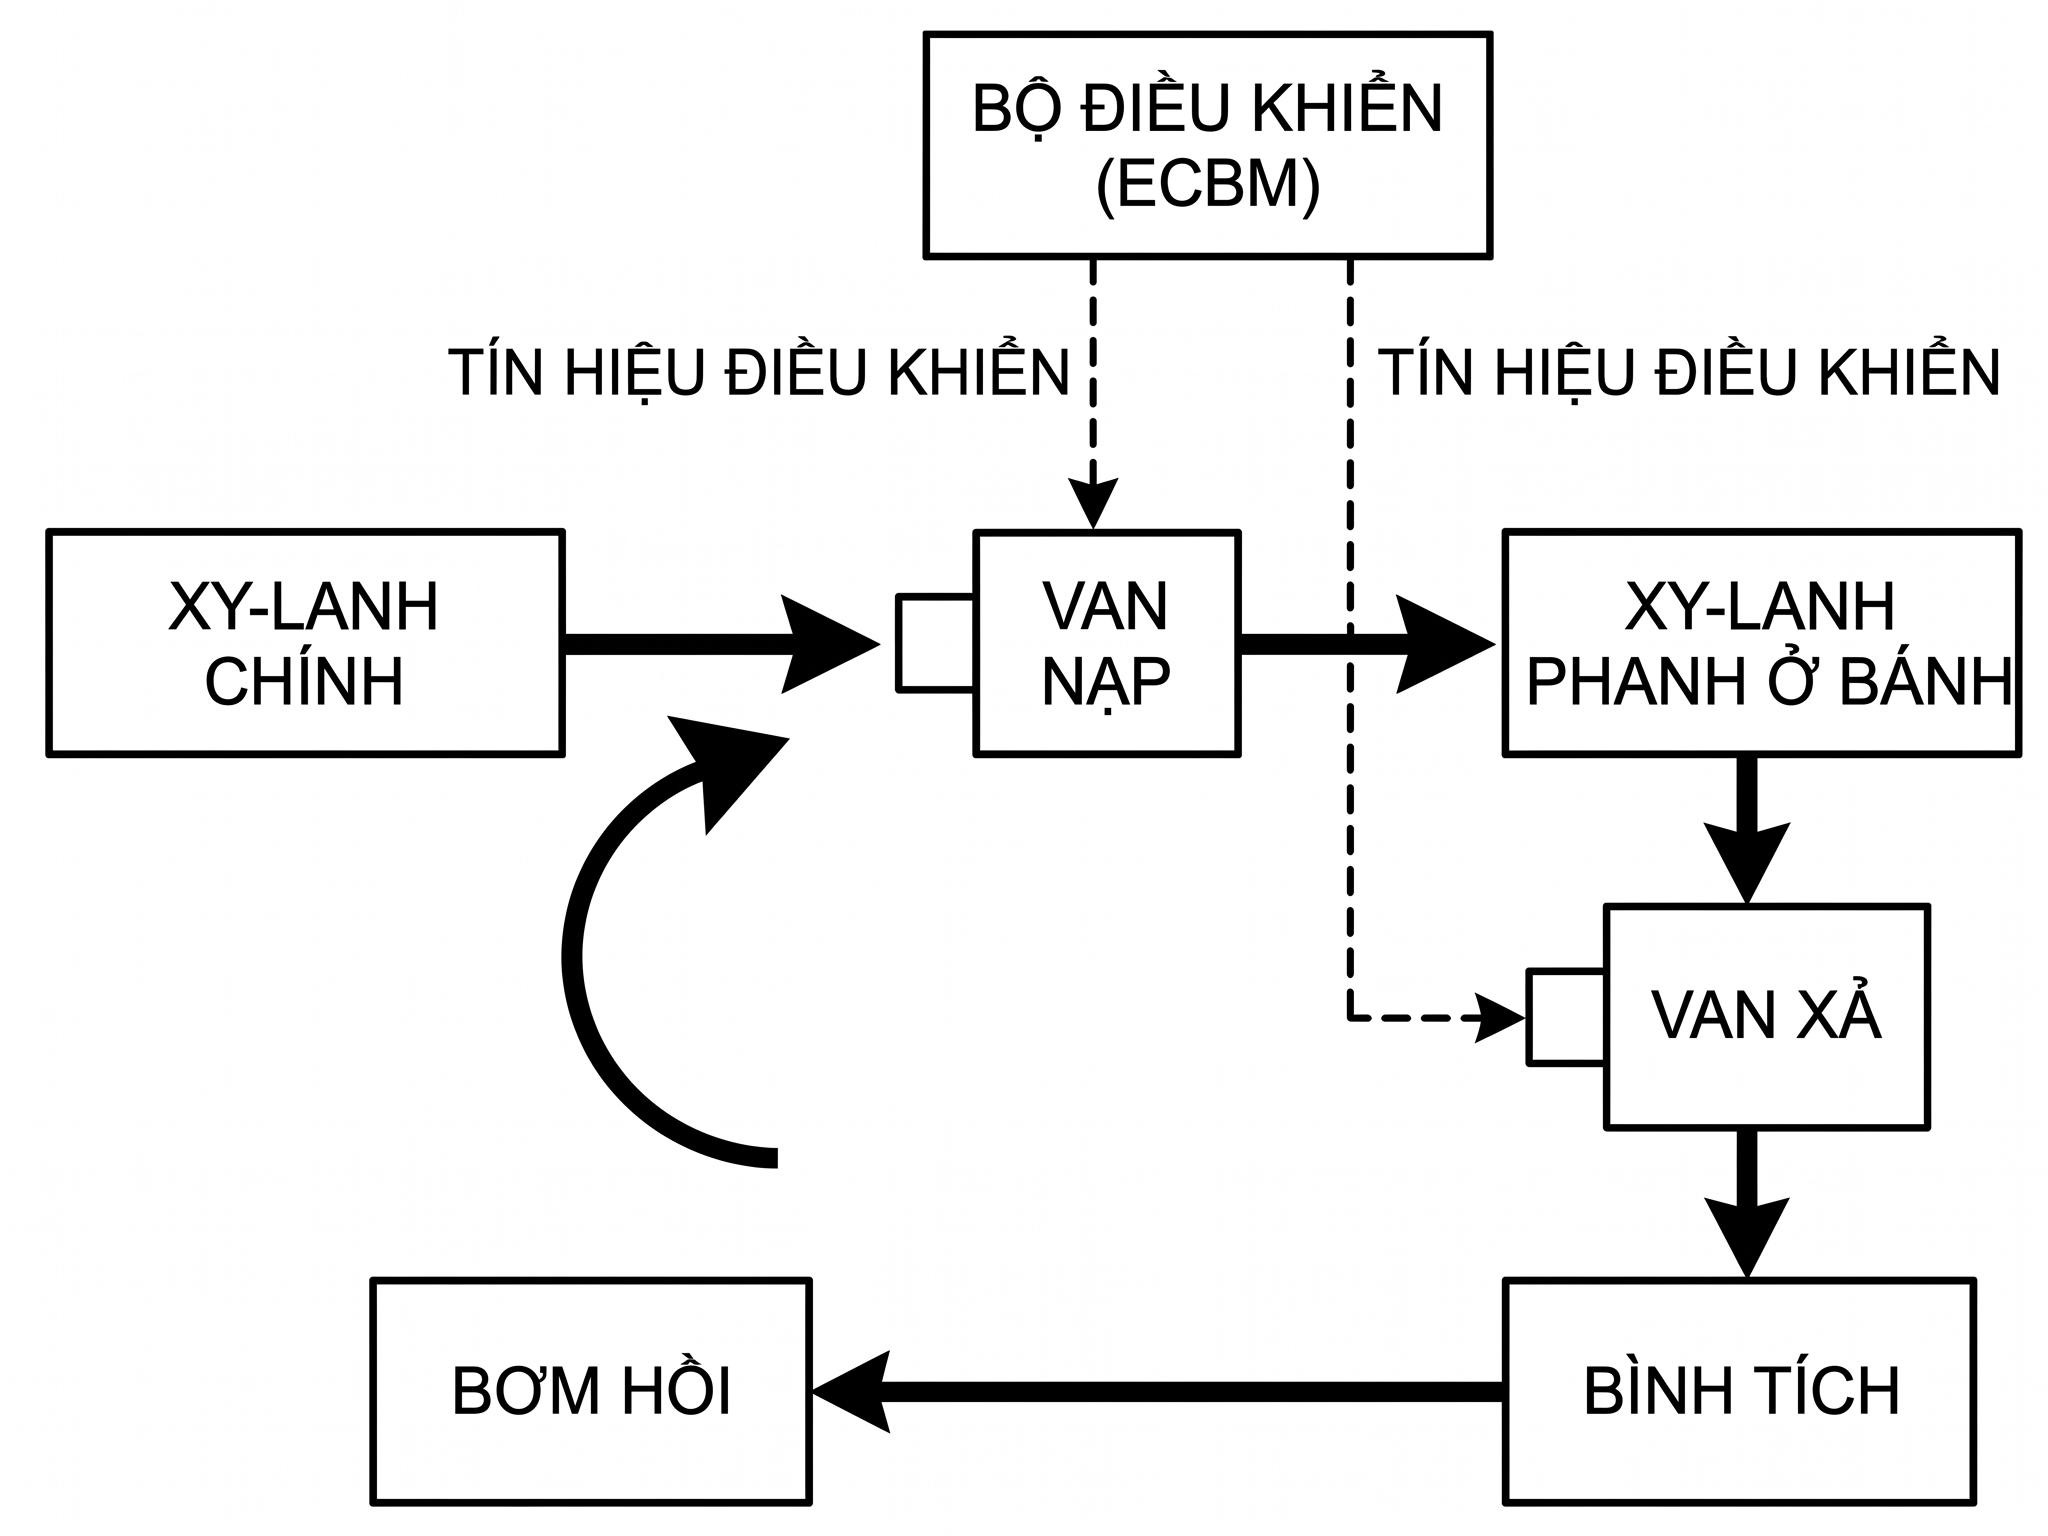
\includegraphics[width=0.65\textwidth]{image/abs_cd3_image2.png}
\end{center}
\figcaption{1}{Sơ đồ cụm van điều biến kiểu van điện từ (van nạp, van xả, bơm hồi).}

Ba trạng thái ấy ghép thành một vòng lặp tự điều chỉnh. Ở mỗi bánh có một cảm biến liên tục đo tốc độ quay và báo về bộ điều khiển. Nếu một bánh chậm hẳn so với các bánh khác (dấu hiệu sắp khóa), bộ điều khiển chuyển van sang giảm áp để nhả bánh. Khi bánh quay lại và bám tốt trở lại, nó chuyển sang tăng áp để phanh tiếp. Khi thấy vừa đủ, nó giữ. Cứ thế van xoay vòng qua ba trạng thái, khiến áp suất phanh dao động lên xuống quanh mức ``vừa đủ để bám mạnh nhất mà chưa khóa''.

Đồ thị áp suất phanh tại một bánh theo thời gian có dạng răng cưa: đi lên (tăng áp), phẳng ngắn ở đỉnh (giữ), rồi đi xuống (giảm áp), sau đó lặp lại. Răng cưa đều đặn cho thấy hệ thống đang hoạt động bình thường.

\tablecaption{2}{Một chu kỳ răng cưa (đồ thị áp suất phanh theo thời gian, minh họa).}
\begin{center}
\renewcommand{\arraystretch}{1.3}
{\small
\setstretch{1.0}%
\begin{tabular}{|>{\centering\arraybackslash}m{2.5cm}|>{\centering\arraybackslash}m{3.5cm}|>{\centering\arraybackslash}m{3.5cm}|}
\hline
\rowcolor{primaryBlue!12}
\textbf{Pha} & \textbf{Khoảng thời gian} & \textbf{Áp suất phanh (bar)} \\
\hline
Tăng áp & 0 -- 20\,ms & 60 lên 100 \\
\hline
Giữ áp & 20 -- 30\,ms & 100 (đỉnh) \\
\hline
Giảm áp & 30 -- 50\,ms & 100 xuống 60 \\
\hline
\end{tabular}
}
\end{center}

Chu kỳ lặp lại từ mốc 50\,ms. Một chu kỳ dài 50\,ms nên hệ điều biến làm $1000 \div 50 = 20$ lần mỗi giây; biên độ dao động áp suất bằng $100 - 60 = 40$\,bar.

Vòng lặp chỉ ổn định khi van phản ứng đúng lúc. Nếu van trễ, tức giảm áp quá muộn (bánh khóa rồi mới nhả) hoặc tăng áp quá sớm (bánh chưa kịp bám đã bị ép tiếp), thì các pha lệch nhịp, biên độ dao động lớn dần, răng cưa méo và dâng cao, hệ mất ổn định.

\tablecaption{3}{So sánh ba kịch bản hoạt động van ABS trong một chu kỳ 50\,ms.}
\begin{center}
\renewcommand{\arraystretch}{1.3}
{\small
\setstretch{1.0}%
\begin{tabular}{|>{\raggedright\arraybackslash}m{4cm}|>{\centering\arraybackslash}m{3.5cm}|>{\raggedright\arraybackslash}m{5.5cm}|}
\hline
\rowcolor{primaryBlue!12}
\textbf{Kịch bản} & \textbf{Biên độ áp suất (bar)} & \textbf{Trạng thái bánh} \\
\hline
Van đúng thời điểm & 40 & Dao động gần ngưỡng tối ưu \\
\hline
Giảm áp trễ 10\,ms & 65 & Bánh khóa cứng rồi mới nhả \\
\hline
Tăng áp trễ 10\,ms & 55 & Bánh trượt khi chưa kịp bám lại \\
\hline
\end{tabular}
}
\end{center}

Tóm lại, van là cơ cấu chấp hành; cảm biến tốc độ thu thập dữ liệu, bộ điều khiển xử lý và ra quyết định. Ba thành phần tạo thành vòng điều khiển kín gồm bốn bước: đo, quyết định, chỉnh áp suất, rồi đo lại; vòng này chạy hàng chục lần mỗi giây, giúp xe vừa dừng ngắn vừa còn lái được.

\hfill\textbf{Nguồn: Nguyễn Nghĩa Đô biên soạn}
\end{readingpassage}

% --- CĐ 3: Câu hỏi ---

\question[Trắc nghiệm]{Trên đồ thị áp suất theo thời gian, đoạn răng cưa đi xuống thể hiện hệ thống đang làm gì?}
\par\vspace{4pt}
\noindent\hangindent=2.2em\hangafter=1\choiceitem{A}{Ép mạnh má phanh vào đĩa.}\par\vspace{4pt}
\noindent\hangindent=2.2em\hangafter=1\choiceitem{B}{Cô lập hoàn toàn bánh xe.}\par\vspace{4pt}
\noindent\hangindent=2.2em\hangafter=1\choiceitem{C}{Nhả bớt lực phanh ở bánh.}\par\vspace{4pt}
\noindent\hangindent=2.2em\hangafter=1\choiceitem{D}{Tạo thêm lực phanh dự phòng.}\par\vspace{4pt}

\question[Trắc nghiệm]{Vì sao phanh ô tô dùng dầu thủy lực thay vì cơ cấu cơ khí?}
\par\vspace{4pt}
\noindent\hangindent=2.2em\hangafter=1\choiceitem{A}{Vì dầu nhẹ hơn kim loại nên giảm trọng lượng xe.}\par\vspace{4pt}
\noindent\hangindent=2.2em\hangafter=1\choiceitem{B}{Vì dầu bôi trơn giúp má phanh không bị mài mòn.}\par\vspace{4pt}
\noindent\hangindent=2.2em\hangafter=1\choiceitem{C}{Vì dầu gần như không nén được nên truyền lực tức thì.}\par\vspace{4pt}
\noindent\hangindent=2.2em\hangafter=1\choiceitem{D}{Vì dầu dẫn nhiệt tốt nên giữ cho đĩa phanh mát hơn.}\par\vspace{4pt}

\question[Trắc nghiệm]{Giả sử cụm van bị kẹt vĩnh viễn ở trạng thái giảm áp. Khi tài xế đạp phanh, bánh xe đó sẽ ra sao?}
\par\vspace{4pt}
\noindent\hangindent=2.2em\hangafter=1\choiceitem{A}{Bánh bị phanh mạnh nhất và khóa cứng ngay.}\par\vspace{4pt}
\noindent\hangindent=2.2em\hangafter=1\choiceitem{B}{Bánh gần như không được phanh vì áp suất luôn bị xả về bình tích.}\par\vspace{4pt}
\noindent\hangindent=2.2em\hangafter=1\choiceitem{C}{Bánh dao động đều quanh vùng bám tối ưu như bình thường.}\par\vspace{4pt}
\noindent\hangindent=2.2em\hangafter=1\choiceitem{D}{Bánh được giữ ở một mức phanh cố định không đổi.}\par\vspace{4pt}

\question[Đúng/Sai]{Các mệnh đề sau về trạng thái van đúng hay sai?}

\vspace{6pt}
\renewcommand{\arraystretch}{1.4}
{\small\setstretch{1.0}
\begin{longtable}{|>{\raggedright\arraybackslash}m{0.72\textwidth}|>{\centering\arraybackslash}m{0.08\textwidth}|>{\centering\arraybackslash}m{0.08\textwidth}|}
\hline
\rowcolor{primaryBlue!12}
\textbf{Nội dung} & \textbf{Đúng} & \textbf{Sai} \\
\hline
\endfirsthead
\hline
\rowcolor{primaryBlue!12}
\textbf{Nội dung} & \textbf{Đúng} & \textbf{Sai} \\
\hline
\endhead
a) Van tăng áp mở đường dầu từ bơm vào xy-lanh bánh. & \tfcircle & \tfcircle \\
\hline
b) Van giữ áp cô lập hoàn toàn: dầu không vào, không ra xy-lanh. & \tfcircle & \tfcircle \\
\hline
c) Van giảm áp giữ nguyên áp suất để chuẩn bị chu kỳ tiếp theo. & \tfcircle & \tfcircle \\
\hline
d) Cả ba trạng thái van có thể hoạt động đồng thời trong một chu kỳ. & \tfcircle & \tfcircle \\
\hline
\end{longtable}
}

\question[Đúng/Sai]{Dựa vào Bảng 3, đánh giá các mệnh đề:}

\vspace{6pt}
\renewcommand{\arraystretch}{1.4}
{\small\setstretch{1.0}
\begin{longtable}{|>{\raggedright\arraybackslash}m{0.72\textwidth}|>{\centering\arraybackslash}m{0.08\textwidth}|>{\centering\arraybackslash}m{0.08\textwidth}|}
\hline
\rowcolor{primaryBlue!12}
\textbf{Nội dung} & \textbf{Đúng} & \textbf{Sai} \\
\hline
\endfirsthead
\hline
\rowcolor{primaryBlue!12}
\textbf{Nội dung} & \textbf{Đúng} & \textbf{Sai} \\
\hline
\endhead
a) Kịch bản đúng thời điểm có biên độ áp suất nhỏ nhất trong ba kịch bản. & \tfcircle & \tfcircle \\
\hline
b) Hai kịch bản trễ đều dẫn đến cùng một hệ quả với bánh xe. & \tfcircle & \tfcircle \\
\hline
c) Cả hai kịch bản trễ đều có biên độ vượt quá 40\,bar. & \tfcircle & \tfcircle \\
\hline
d) Tăng áp trễ tạo ra biên độ lớn hơn giảm áp trễ. & \tfcircle & \tfcircle \\
\hline
\end{longtable}
}

\question[Điền khuyết]{Xét một lần phanh gấp trên đường trơn.\\[3pt]
\textit{(Điền số (làm tròn đến hàng đơn vị) vào chỗ trống.)}}
\vspace{2pt}
\setstretch{1.4}
Theo Bảng 2, mỗi chu kỳ răng cưa dài 50\,ms, nên trong một giây hệ điều biến xoay vòng trạng thái (1)\,\dropbox[2cm] lần. Nếu pha phanh gấp này kéo dài 0,5 giây, đồ thị áp suất sẽ hoàn thành (2)\,\dropbox[2cm] chu kỳ răng cưa. Giả sử kỹ sư nâng cấp van bằng cách bỏ hẳn pha giữ áp (van chỉ luân phiên tăng áp và giảm áp, thời gian mỗi pha giữ nguyên như Bảng 2) thì tần số điều biến tăng lên thành (3)\,\dropbox[2cm] lần mỗi giây.

\question[Ghép đôi]{Ghép mỗi động tác chân ở Cột A với trạng thái van ở Cột B.}

\vspace{6pt}
\setstretch{1.3}

\textit{Cột B:}
\vspace{-6pt}
\par\vspace{4pt}
\noindent\hangindent=2.2em\hangafter=1\choiceitem{A}{Giữ áp}\par\vspace{4pt}
\noindent\hangindent=2.2em\hangafter=1\choiceitem{B}{Khóa áp}\par\vspace{4pt}
\noindent\hangindent=2.2em\hangafter=1\choiceitem{C}{Tăng áp}\par\vspace{4pt}
\noindent\hangindent=2.2em\hangafter=1\choiceitem{D}{Giảm áp}\par\vspace{4pt}

\vspace{6pt}

\renewcommand{\arraystretch}{1.6}
{\small\setstretch{1.0}
\begin{longtable}{|>{\raggedright\arraybackslash}m{0.55\textwidth}|>{\centering\arraybackslash}m{0.28\textwidth}|}
\hline
\rowcolor{primaryBlue!12}
\multicolumn{1}{|c|}{\cellcolor{primaryBlue!12}\textbf{Cột A}} & \cellcolor{primaryBlue!12}\textbf{Cột B} \\
\hline
\endfirsthead
\hline
\rowcolor{primaryBlue!12}
\multicolumn{1}{|c|}{\cellcolor{primaryBlue!12}\textbf{Cột A}} & \cellcolor{primaryBlue!12}\textbf{Cột B} \\
\hline
\endhead
1. Đạp mạnh thêm chân phanh & \dropbox[2.5cm] \\
\hline
2. Giữ chân phanh yên & \dropbox[2.5cm] \\
\hline
3. Nhấc bớt chân phanh & \dropbox[2.5cm] \\
\hline
\end{longtable}
}

\question[Ghép đôi]{Ghép mỗi hiện tượng ở Cột A với kết luận đúng ở Cột B.}

\vspace{6pt}
\setstretch{1.3}

\textit{Cột B:}
\vspace{-6pt}
\par\vspace{4pt}
\noindent\hangindent=2.2em\hangafter=1\choiceitem{A}{Hệ đang chạy bình thường}\par\vspace{4pt}
\noindent\hangindent=2.2em\hangafter=1\choiceitem{B}{Van phản ứng lệch pha, hệ mất ổn định}\par\vspace{4pt}
\noindent\hangindent=2.2em\hangafter=1\choiceitem{C}{Van kẹt ở trạng thái giữ áp}\par\vspace{4pt}
\noindent\hangindent=2.2em\hangafter=1\choiceitem{D}{Bánh bị khóa cứng một lúc rồi mới được nhả}\par\vspace{4pt}
\noindent\hangindent=2.2em\hangafter=1\choiceitem{E}{Bánh bị ép khi chưa kịp lấy lại độ bám, gây trượt}\par\vspace{4pt}
\noindent\hangindent=2.2em\hangafter=1\choiceitem{F}{Van đang tạo thêm lực phanh cực lớn}\par\vspace{4pt}

\vspace{6pt}

\renewcommand{\arraystretch}{1.6}
{\small\setstretch{1.0}
\begin{longtable}{|>{\raggedright\arraybackslash}m{0.55\textwidth}|>{\centering\arraybackslash}m{0.28\textwidth}|}
\hline
\rowcolor{primaryBlue!12}
\multicolumn{1}{|c|}{\cellcolor{primaryBlue!12}\textbf{Cột A}} & \cellcolor{primaryBlue!12}\textbf{Cột B} \\
\hline
\endfirsthead
\hline
\rowcolor{primaryBlue!12}
\multicolumn{1}{|c|}{\cellcolor{primaryBlue!12}\textbf{Cột A}} & \cellcolor{primaryBlue!12}\textbf{Cột B} \\
\hline
\endhead
1. Răng cưa đều đặn, biên độ ổn định & \dropbox[2.5cm] \\
\hline
2. Răng cưa méo, biên độ dâng cao dần & \dropbox[2.5cm] \\
\hline
3. Áp suất một bánh vọt lên rồi nằm im ở đỉnh, không tụt & \dropbox[2.5cm] \\
\hline
4. Lệnh giảm áp đến quá muộn & \dropbox[2.5cm] \\
\hline
5. Lệnh tăng áp đến quá sớm & \dropbox[2.5cm] \\
\hline
\end{longtable}
}

\question[Kéo thả]{Kéo các cụm từ trong kho vào chỗ trống cho phù hợp:}
\vspace{-4pt}
\dragitems{
\centering
    \dragitem{không nén được} \dragitem{giảm áp suất} \dragitem{áp suất dầu}\\[1pt]
    \dragitem{áp suất khí} \dragitem{truyền trực tiếp}
}

\setstretch{1.4}
Phanh ô tô là hệ thủy lực, nơi lực đạp không (1)\,\dropbox[2.5cm] bằng một cơ cấu cứng. Ống dẫn chứa dầu phanh, một chất lỏng gần như (2)\,\dropbox[2.5cm]. Nhờ đó, lực ép ở một đầu được dẫn truyền dưới dạng (3)\,\dropbox[2.5cm] tới má phanh.

\question[Kéo thả]{Kéo các cụm từ trong kho vào chỗ trống cho phù hợp:}
\vspace{-4pt}
\dragitems{
\centering
    \dragitem{quyết định} \dragitem{phanh chết} \dragitem{đo lại}\\[1pt]
    \dragitem{vòng điều khiển hở} \dragitem{nhả -- giữ -- ép}
}

\setstretch{1.4}
ABS thông minh vì không (1)\,\dropbox[2cm] một lần rồi thôi, mà áp dụng vòng lặp (2)\,\dropbox[3cm] áp suất liên tục. Cảm biến đo đạc, báo cho não bộ (3)\,\dropbox[2cm], van điều tiết áp suất làm bánh thay đổi, rồi cảm biến (4)\,\dropbox[2cm] để tinh chỉnh.
% ============================================================
% CHỦ ĐỀ 4: LỰC PHANH, MA SÁT VÀ ĐỘ TRƯỢT
% ============================================================
\newpage
\setcounter{qcounter}{0}

\phantomsection\label{b2_cd3_4}
\begin{topicbox}{\large CHỦ ĐỀ 4: LỰC PHANH, MA SÁT VÀ ĐỘ TRƯỢT}
\vspace{8pt}
\textit{Đọc đoạn văn sau và trả lời các câu hỏi.}
\vspace{6pt}
\end{topicbox}

\begin{readingpassage}[]
\setstretch{1.3}

Khi người lái đạp phanh, yếu tố quyết định xe dừng nhanh hay chậm không phải lực đạp mà là ma sát giữa lốp và mặt đường. Ma sát này có hai trạng thái khác nhau. Khi bánh xe còn lăn, điểm lốp chạm đường gần như đứng yên so với mặt đường trong thời gian tiếp xúc, nên lực bám thuộc loại ma sát nghỉ và đạt giá trị lớn. Khi bánh bị khóa cứng và trượt lê trên đường, lực bám giảm xuống mức ma sát trượt, thấp hơn đáng kể so với ma sát nghỉ. Xe phanh với bánh trượt vừa có quãng đường dừng dài hơn, vừa mất khả năng chuyển hướng.

Mức độ chuyển tiếp giữa hai trạng thái được lượng hóa bằng đại lượng độ trượt. Gọi $v$ là vận tốc thân xe, $\omega$ là tốc độ quay của bánh và $R$ là bán kính lốp, độ trượt được tính bằng:

\begin{center}
$\displaystyle \sigma = \frac{v - \omega R}{v}$
\end{center}

Vận tốc tịnh tiến $v$ có đơn vị là m/s. $\omega$ có đơn vị là rad/s. Tích $\omega R$ (vận tốc dài tiếp tuyến) có đơn vị là m/s. Bánh lăn hoàn hảo có $v = \omega R$ nên $\sigma = 0$. Bánh khóa hoàn toàn có $\omega = 0$ nên $\sigma = 1$.

\begin{center}
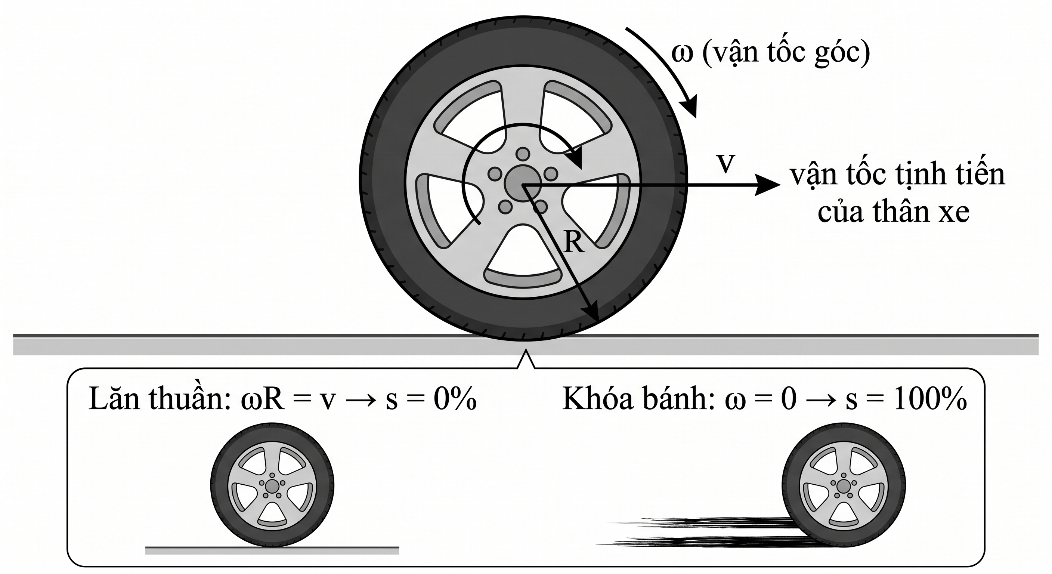
\includegraphics[width=0.55\textwidth]{image/abs_cd4_image2.png}
\end{center}
\figcaption{1}{Vận tốc tịnh tiến của thân xe và vận tốc quay của bánh.}

Hệ số bám $\mu$ không cố định mà thay đổi theo độ trượt. Khi $\sigma$ tăng từ 0, $\mu$ tăng rất nhanh, đạt đỉnh trong khoảng $\sigma = 10\%$ đến $20\%$, rồi giảm dần nếu bánh tiếp tục trượt tới 100\%. Vùng đỉnh này là nơi lốp bám đường tốt nhất. Hệ thống chống bó cứng phanh hoạt động bằng cách duy trì độ trượt dao động quanh vùng đỉnh để giữ $\mu$ ở mức cao nhất.

\begin{center}
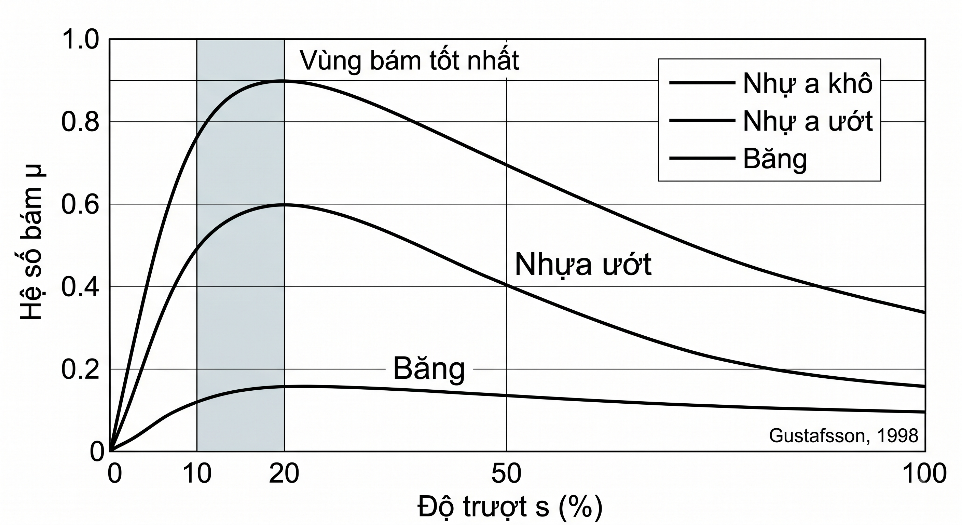
\includegraphics[width=0.55\textwidth]{image/abs_cd4_image3.png}
\end{center}
\figcaption{2}{Đường cong hệ số bám $\mu$ theo độ trượt $\sigma$ (Gustafsson, 1998).}

Độ dốc của đoạn đầu đường cong (phần đi lên trước khi tới đỉnh) cho phép nhận diện loại mặt đường: trên đường nhựa khô đoạn này dốc đứng, trên băng nó thoai thoải. Nhờ đọc độ dốc đó từ chính tín hiệu tốc độ bánh mà cảm biến ABS thu được, hệ thống có thể nhận diện loại mặt đường mà không cần lắp thêm cảm biến riêng (Gustafsson, 1998).

\tablecaption{1}{Hệ số bám cực đại $\mu_{\text{đỉnh}}$ và hệ số bám khi trượt $\mu_{\text{trượt}}$ trên các mặt đường.}
\setstretch{1.0}%
\begin{center}
\begin{tabular}{|c|c|c|}
\hline
\rowcolor{primaryBlue!12}
\textbf{Mặt đường} & $\boldsymbol{\mu_{\textbf{đỉnh}}}$ \textbf{(bám tốt nhất)} & $\boldsymbol{\mu_{\textbf{trượt}}}$ \textbf{(bánh khóa)} \\
\hline
Nhựa khô & 0,90 & 0,65 \\
\hline
Nhựa ướt & 0,60 & 0,40 \\
\hline
Băng & 0,15 & 0,08 \\
\hline
\end{tabular}
\end{center}

Quãng đường phanh gắn trực tiếp với $\mu$ qua công thức $d = \dfrac{v^2}{2\mu g}$, với $g = 9{,}8\;\text{m/s}^2$. Một xe chạy 20\,m/s trên nhựa khô, nếu giữ được $\mu_{\text{đỉnh}} = 0{,}90$ thì cần khoảng 22,7\,m để dừng; nếu để bánh khóa và $\mu$ tụt về $\mu_{\text{trượt}} = 0{,}65$ thì quãng đường kéo dài tới 31,4\,m. Chênh lệch gần chín mét cho thấy việc duy trì hệ số bám tối ưu hiệu quả hơn so với tăng lực phanh.

\hfill\textbf{Nguồn: Nguyễn Nghĩa Đô biên soạn}
\end{readingpassage}

% --- Câu 1: Trắc nghiệm ---
\question[Trắc nghiệm]{Dựa vào Hình 1 và văn bản, phát biểu nào sau đây mô tả chính xác nhất mối liên hệ giữa trạng thái của bánh xe và độ trượt $\sigma$?}
\par\vspace{4pt}
\noindent\hangindent=2.2em\hangafter=1\choiceitem{A}{Bánh lăn thuần có $\sigma = 0$, trong khi bánh trượt thuần có $\sigma = 1$.}\par\vspace{4pt}
\noindent\hangindent=2.2em\hangafter=1\choiceitem{B}{Bánh lăn thuần có $\sigma = 1$, trong khi bánh trượt thuần có $\sigma = 0$.}\par\vspace{4pt}
\noindent\hangindent=2.2em\hangafter=1\choiceitem{C}{Cả lăn thuần và trượt thuần đều duy trì độ trượt $\sigma$ ở mức $10\text{--}20\%$.}\par\vspace{4pt}
\noindent\hangindent=2.2em\hangafter=1\choiceitem{D}{Khi bánh xe lăn thuần, hệ số bám đường luôn đạt giá trị cực đại $\mu_{\text{đỉnh}}$.}\par\vspace{4pt}

% --- Câu 2: Trắc nghiệm ---
\question[Trắc nghiệm]{Một ô tô đang di chuyển với vận tốc tịnh tiến $v = 20$\,m/s. Hệ thống cảm biến đo được bán kính lốp $R = 0{,}3$\,m và tốc độ quay của bánh xe $\omega = 56$\,rad/s. Trạng thái bám đường của bánh xe lúc này là gì?}
\par\vspace{4pt}
\noindent\hangindent=2.2em\hangafter=1\choiceitem{A}{Bánh xe đang lăn hoàn hảo với độ trượt $\sigma = 0$, an toàn tuyệt đối.}\par\vspace{4pt}
\noindent\hangindent=2.2em\hangafter=1\choiceitem{B}{Bánh xe đang bị khóa cứng với độ trượt $\sigma = 1$, xe mất kiểm soát.}\par\vspace{4pt}
\noindent\hangindent=2.2em\hangafter=1\choiceitem{C}{Bánh xe đang có độ trượt $\sigma = 16\%$, nằm trong vùng bám đường tốt nhất.}\par\vspace{4pt}
\noindent\hangindent=2.2em\hangafter=1\choiceitem{D}{Bánh xe đang trượt nghịch với độ trượt âm $\sigma < 0$, gia tốc ngược chiều.}\par\vspace{4pt}

% --- Câu 3: Trắc nghiệm ---
\question[Trắc nghiệm]{Một học sinh quan sát Hình 2 (Đường cong Gustafsson) và đưa ra các dự đoán về trạng thái của lốp xe khi tài xế đột ngột đạp phanh hết cỡ khiến bánh xe bị khóa hoàn toàn. Phân tích nào sau đây là đúng với sự biến thiên của hệ số bám $\mu$?}
\par\vspace{4pt}
\noindent\hangindent=2.2em\hangafter=1\choiceitem{A}{Từ $\sigma = 0$ đến $\sigma = 1$, hệ số bám liên tục tăng dần đều cho đến khi khóa.}\par\vspace{4pt}
\noindent\hangindent=2.2em\hangafter=1\choiceitem{B}{Lực bám sẽ đi từ ma sát nghỉ rất nhỏ, lên đỉnh rồi duy trì ổn định.}\par\vspace{4pt}
\noindent\hangindent=2.2em\hangafter=1\choiceitem{C}{Hệ số bám tăng vọt lên đỉnh ở mức trượt $10\text{--}20\%$ rồi giảm dần đi.}\par\vspace{4pt}
\noindent\hangindent=2.2em\hangafter=1\choiceitem{D}{Khi vừa khóa cứng, hệ số bám tụt thẳng về $\sigma = 0$ và xe dừng ngay lập tức.}\par\vspace{4pt}

% --- Câu 4: Trắc nghiệm ---
\question[Trắc nghiệm]{Một chiếc xe chạy với vận tốc $v = 20$\,m/s trên mặt đường nhựa ướt. Xe gặp sự cố hỏng phanh ABS, khiến bánh xe bị khóa hoàn toàn ngay khi người lái đạp phanh. Hậu quả về quãng đường phanh (làm tròn đến 1 chữ số sau dấu thập phân) được phân tích như thế nào?}
\par\vspace{4pt}
\noindent\hangindent=2.2em\hangafter=1\choiceitem{A}{Do lốp không trượt, hệ số bám duy trì ở đỉnh $\mu = 0{,}60$, quãng đường phanh dài $d \approx 34{,}0$\,m.}\par\vspace{4pt}
\noindent\hangindent=2.2em\hangafter=1\choiceitem{B}{Quên bình phương vận tốc, quãng đường phanh sai lệch chỉ còn khoảng $d \approx 2{,}6$\,m.}\par\vspace{4pt}
\noindent\hangindent=2.2em\hangafter=1\choiceitem{C}{Do bánh khóa cứng, hệ số bám tụt về trượt $\mu = 0{,}40$, quãng đường phanh dài $d \approx 51{,}0$\,m.}\par\vspace{4pt}
\noindent\hangindent=2.2em\hangafter=1\choiceitem{D}{Nếu tính nhầm sang đường khô với hệ số bám là $\mu = 0{,}65$, quãng đường phanh sẽ dài khoảng $d \approx 31{,}4$\,m.}\par\vspace{4pt}

% --- Câu 5: Đúng/Sai ---
\question[Đúng/Sai]{Phân tích các số liệu về hệ số bám trên các mặt đường tại Bảng 1.}

\vspace{6pt}
\renewcommand{\arraystretch}{1.4}
{\small\setstretch{1.0}
\begin{longtable}{|>{\raggedright\arraybackslash}m{0.72\textwidth}|>{\centering\arraybackslash}m{0.08\textwidth}|>{\centering\arraybackslash}m{0.08\textwidth}|}
\hline
\rowcolor{primaryBlue!12}
\textbf{Nội dung} & \textbf{Đúng} & \textbf{Sai} \\
\hline
\endfirsthead
\hline
\rowcolor{primaryBlue!12}
\textbf{Nội dung} & \textbf{Đúng} & \textbf{Sai} \\
\hline
\endhead
a) Trên mặt đường nhựa ướt, việc để bánh xe bị khóa làm tụt 0,20 giá trị hệ số bám so với mức tối ưu. & \tfcircle & \tfcircle \\
\hline
b) Giá trị bám đường tốt nhất trên mặt băng tuyết vẫn thấp hơn ma sát khi xe trượt hoàn toàn trên nhựa ướt. & \tfcircle & \tfcircle \\
\hline
c) Nếu cùng chạy với một vận tốc, quãng đường phanh trên mặt băng khi khóa bánh sẽ gấp hơn 10 lần quãng đường phanh trên nhựa khô khi ABS hoạt động. & \tfcircle & \tfcircle \\
\hline
d) Độ sụt giảm tương đối của hệ số bám (tính bằng phần trăm từ đỉnh xuống trượt) trên mặt nhựa khô là lớn nhất trong ba loại mặt đường. & \tfcircle & \tfcircle \\
\hline
\end{longtable}
}

% --- Câu 6: Đúng/Sai ---
\question[Đúng/Sai]{Kết hợp công thức độ trượt và biểu đồ ma sát, đánh giá các tình huống vận hành sau đây.}

\vspace{6pt}
\renewcommand{\arraystretch}{1.4}
{\small\setstretch{1.0}
\begin{longtable}{|>{\raggedright\arraybackslash}m{0.72\textwidth}|>{\centering\arraybackslash}m{0.08\textwidth}|>{\centering\arraybackslash}m{0.08\textwidth}|}
\hline
\rowcolor{primaryBlue!12}
\textbf{Nội dung} & \textbf{Đúng} & \textbf{Sai} \\
\hline
\endfirsthead
\hline
\rowcolor{primaryBlue!12}
\textbf{Nội dung} & \textbf{Đúng} & \textbf{Sai} \\
\hline
\endhead
a) Bánh xe lăn hoàn hảo có hệ số bám cao nhất vì lúc này điểm tiếp xúc đứng yên so với mặt đường. & \tfcircle & \tfcircle \\
\hline
b) Khi người lái đạp phanh, nếu $\sigma$ liên tục tăng từ $20\%$ lên $100\%$, quãng đường phanh sẽ ngày càng bị kéo dài ra so với việc giữ $\sigma$ ở mức $15\%$. & \tfcircle & \tfcircle \\
\hline
c) Nếu tín hiệu tốc độ bánh xe gửi về $\omega$ luôn đáp ứng phương trình $\omega = \dfrac{0{,}85v}{R}$, hệ thống ABS đang duy trì bám đường tối ưu. & \tfcircle & \tfcircle \\
\hline
d) Hệ thống của xe chạy trên băng tuyết có thể đoán loại đường bằng cách đo giá trị trượt thuần tại $\sigma = 100\%$. & \tfcircle & \tfcircle \\
\hline
\end{longtable}
}

% --- Câu 7: Điền khuyết ---
\question[Điền khuyết]{Dựa vào Bảng 1 và công thức đã cho, hãy phân tích bài toán dừng xe khẩn cấp từ vận tốc $v = 20$\,m/s trên đường nhựa ướt. (Làm tròn đến 1 chữ số sau dấu thập phân).}

\setstretch{1.4}
\begin{itemize}[leftmargin=*, itemsep=5pt, topsep=0pt, partopsep=0pt, parsep=0pt, label=\textcolor{primaryBlue}{\textbullet}]
\item Nếu phanh ABS hoạt động, hệ số bám đạt đỉnh bằng (1)\,\dropbox[1.5cm], quãng đường xe cần để dừng lại là (2)\,\dropbox[2cm]\,m.
\item Trong trường hợp ABS hỏng khiến bánh xe bị khóa, hệ số bám sụt xuống còn (3)\,\dropbox[1.5cm], làm quãng đường phanh bị kéo dài thêm một khoảng chênh lệch là (4)\,\dropbox[2cm]\,m.
\end{itemize}

% --- Câu 8: Ghép đôi ---
\question[Ghép đôi]{Một kỹ sư đang thiết kế phần mềm phanh cho xe tự hành. Hãy ghép các điều kiện vận hành tại Cột A (với vận tốc ban đầu không đổi $v = 10$\,m/s) với kết quả quãng đường phanh tương ứng tại Cột B.}

\vspace{6pt}
\setstretch{1.3}

\textit{Cột B:}
\vspace{-6pt}
\par\vspace{4pt}
\noindent\hangindent=2.2em\hangafter=1\choiceitem{A}{Khoảng 5,7\,m}\par\vspace{4pt}
\noindent\hangindent=2.2em\hangafter=1\choiceitem{B}{Bất khả thi với dữ liệu ở Bảng 1}\par\vspace{4pt}
\noindent\hangindent=2.2em\hangafter=1\choiceitem{C}{Khoảng 12,8\,m}\par\vspace{4pt}
\noindent\hangindent=2.2em\hangafter=1\choiceitem{D}{Khoảng 34,0\,m}\par\vspace{4pt}
\noindent\hangindent=2.2em\hangafter=1\choiceitem{E}{Khoảng 63,8\,m}\par\vspace{4pt}

\vspace{6pt}

\renewcommand{\arraystretch}{1.6}
{\small\setstretch{1.0}
\begin{longtable}{|>{\raggedright\arraybackslash}m{0.55\textwidth}|>{\centering\arraybackslash}m{0.28\textwidth}|}
\hline
\rowcolor{primaryBlue!12}
\multicolumn{1}{|c|}{\cellcolor{primaryBlue!12}\textbf{Cột A}} & \cellcolor{primaryBlue!12}\textbf{Cột B} \\
\hline
\endfirsthead
\hline
\rowcolor{primaryBlue!12}
\multicolumn{1}{|c|}{\cellcolor{primaryBlue!12}\textbf{Cột A}} & \cellcolor{primaryBlue!12}\textbf{Cột B} \\
\hline
\endhead
1. Xe phanh khẩn cấp làm khóa bánh trên bề mặt nhựa ướt & \dropbox[2.5cm] \\
\hline
2. Phanh ABS kích hoạt duy trì bám đường tối ưu trên băng & \dropbox[2.5cm] \\
\hline
3. Phanh ABS kích hoạt duy trì bám đường tối ưu trên nhựa khô & \dropbox[2.5cm] \\
\hline
4. Yêu cầu xe bắt buộc phải dừng hẳn trong đúng 10\,mét & \dropbox[2.5cm] \\
\hline
\end{longtable}
}

% --- Câu 9: Ghép đôi ---
\question[Ghép đôi]{Liên kết các vị trí trên trục hoành của Hình 2 (Đường cong Gustafsson) ở Cột A với ý nghĩa vật lý tương ứng của bề mặt lốp ở Cột B.}

\vspace{6pt}
\setstretch{1.3}

\textit{Cột B:}
\vspace{-6pt}
\par\vspace{4pt}
\noindent\hangindent=2.2em\hangafter=1\choiceitem{A}{Lực ma sát tụt xuống trạng thái ma sát trượt thấp hơn đỉnh}\par\vspace{4pt}
\noindent\hangindent=2.2em\hangafter=1\choiceitem{B}{Bánh lăn hoàn hảo, điểm lốp chạm đường gần như đứng yên so với mặt đường}\par\vspace{4pt}
\noindent\hangindent=2.2em\hangafter=1\choiceitem{C}{Hệ số bám đạt đỉnh, ma sát nghỉ phát huy tối đa hiệu quả}\par\vspace{4pt}
\noindent\hangindent=2.2em\hangafter=1\choiceitem{D}{Đường cong dốc lên, độ dốc này cho biết xe đang chạy trên băng hay đường khô}\par\vspace{4pt}
\noindent\hangindent=2.2em\hangafter=1\choiceitem{E}{Hệ thống cảm biến ABS bị vô hiệu hóa hoàn toàn}\par\vspace{4pt}

\vspace{6pt}

\renewcommand{\arraystretch}{1.6}
{\small\setstretch{1.0}
\begin{longtable}{|>{\raggedright\arraybackslash}m{0.55\textwidth}|>{\centering\arraybackslash}m{0.28\textwidth}|}
\hline
\rowcolor{primaryBlue!12}
\multicolumn{1}{|c|}{\cellcolor{primaryBlue!12}\textbf{Cột A}} & \cellcolor{primaryBlue!12}\textbf{Cột B} \\
\hline
\endfirsthead
\hline
\rowcolor{primaryBlue!12}
\multicolumn{1}{|c|}{\cellcolor{primaryBlue!12}\textbf{Cột A}} & \cellcolor{primaryBlue!12}\textbf{Cột B} \\
\hline
\endhead
1. Giai đoạn $\sigma$ đi từ $0\%$ tiến dần tới $10\%$ & \dropbox[2.5cm] \\
\hline
2. Tại đúng điểm $\sigma = 0\%$ & \dropbox[2.5cm] \\
\hline
3. Tại vùng $\sigma = 10\%$ đến $20\%$ & \dropbox[2.5cm] \\
\hline
4. Tại điểm mút $\sigma = 100\%$ & \dropbox[2.5cm] \\
\hline
\end{longtable}
}

% --- Câu 10: Kéo thả ---
\question[Kéo thả]{Hoàn thành đoạn phân tích sau đây về nguyên lý thông minh của hệ thống chống bó cứng phanh bằng cách kéo các cụm từ thích hợp vào ô trống.}
\vspace{-4pt}
\dragitems{
\centering
    \dragitem{hệ số bám đỉnh} \dragitem{đi xuống sau đỉnh} \dragitem{dốc đứng}\\[1pt]
    \dragitem{thoai thoải} \dragitem{đi lên trước đỉnh} \dragitem{ma sát trượt} \dragitem{độ trượt 100\%}
}

\setstretch{1.4}
Thay vì lắp thêm cảm biến đo thời tiết, hệ thống xe có thể nhận diện mặt đường dựa vào tín hiệu tốc độ bánh xe. Bằng cách tính toán độ dốc của đoạn (1)\,\dropbox[2.5cm] trên đường cong ma sát, xe phân biệt được các loại đường. Nếu đoạn này (2)\,\dropbox[2cm], hệ thống chẩn đoán xe đang chạy trên nhựa khô. Ngược lại, nếu đường cong (3)\,\dropbox[2cm], mặt đường có thể là băng tuyết. Kỹ thuật này giúp ABS điều chỉnh lực phanh quanh vùng (4)\,\dropbox[2.5cm] để tối ưu hóa quãng đường dừng mà xe không bị mất khả năng chuyển hướng.

% ============================================================
% CHỦ ĐỀ 5: NGHỊCH LÝ MẶT ĐƯỜNG
% ============================================================
\newpage
\setcounter{qcounter}{0}

\phantomsection\label{b2_cd3_5}
\begin{topicbox}{\large CHỦ ĐỀ 5: NGHỊCH LÝ MẶT ĐƯỜNG}
\vspace{8pt}
\textit{Đọc đoạn văn sau và trả lời các câu hỏi.}
\vspace{6pt}
\end{topicbox}

\begin{readingpassage}[]
\setstretch{1.3}

Trong một thử nghiệm, cùng một chiếc xe được cho phanh gấp từ tốc độ 80\,km/h trên năm loại mặt đường, mỗi lần đo ở hai chế độ: kích hoạt ABS hoặc khóa cứng bánh (phanh truyền thống). Quãng đường từ thời điểm tác động phanh đến khi xe dừng hẳn được ghi trong Bảng 1.

\tablecaption{1}{Quãng đường phanh từ 80\,km/h, so sánh có ABS và khóa bánh.}
\setstretch{1.0}%
\begin{center}
\begin{tabular}{|c|c|c|c|}
\hline
\rowcolor{primaryBlue!12}
\textbf{Mặt đường} & \textbf{Có ABS (m)} & \textbf{Khóa bánh (m)} & \textbf{Chênh lệch (m)} \\
\hline
Nhựa khô & 27 & 29 & ABS ngắn hơn 2 \\
\hline
Nhựa ướt & 39 & 45 & ABS ngắn hơn 6 \\
\hline
Sỏi rời & 32 & 27 & ABS dài hơn 5 \\
\hline
Tuyết nén & 60 & 53 & ABS dài hơn 7 \\
\hline
Băng & 140 & 138 & xấp xỉ 0 \\
\hline
\end{tabular}
\end{center}

Trên hai mặt đường cứng là nhựa khô và nhựa ướt, ABS rút ngắn quãng đường đúng như mong đợi, vì nó giữ bánh ở vùng bám tốt nhất thay vì để trượt. Trên sỏi rời và tuyết nén, kết quả đảo chiều: xe bị khóa bánh lại dừng sớm hơn.

Nguyên nhân nằm ở một cơ chế chỉ xuất hiện trên bề mặt rời. Khi bánh bị khóa và trượt trên lớp sỏi hay tuyết rời, nó vun vật liệu thành một nêm nhỏ tích tụ phía trước lốp. Nêm vật liệu này cản trở chuyển động và tạo thêm lực cản, cộng vào ma sát trượt vốn đã có. ABS không cho bánh khóa nên không đắp được nêm, dẫn tới quãng đường dài hơn.

Nghịch lý này có thể dẫn đến kết luận rằng nên tắt ABS trên bề mặt rời, tuy nhiên quãng đường phanh chỉ phản ánh một phần bài toán an toàn. Xe khóa bánh dừng sớm hơn vài mét, nhưng trong quá trình trượt xe mất khả năng chuyển hướng do bánh trước khóa cứng khiến vô lăng không còn tác dụng. Xe có ABS dừng chậm hơn nhưng vẫn duy trì khả năng chuyển hướng để tránh chướng ngại. Ở phần lớn tình huống thực tế, khả năng tránh va chạm có ý nghĩa an toàn lớn hơn vài mét quãng đường phanh.

Câu hỏi ``khi nào phanh truyền thống thắng'' vì thế có lời giải hẹp: khi mặt đường rời, xe đi thẳng và người lái không cần chuyển hướng. Ngoài ba điều kiện đó, khả năng duy trì chuyển hướng mang lại ưu thế cho ABS. Giới hạn cuối cùng vẫn là bám đường, vì không hệ thống phanh nào tạo ra lực bám lớn hơn mức mà lốp và mặt đường cho phép.

\hfill\textbf{Nguồn: Nguyễn Nghĩa Đô biên soạn}
\end{readingpassage}

% --- Câu 1: Trắc nghiệm ---
\question[Trắc nghiệm]{Theo Bảng 1, trên loại mặt đường nào hệ thống ABS làm tăng quãng đường phanh nhiều nhất so với phanh khóa bánh truyền thống?}
\par\vspace{4pt}
\noindent\hangindent=2.2em\hangafter=1\choiceitem{A}{Đường nhựa ướt.}\par\vspace{4pt}
\noindent\hangindent=2.2em\hangafter=1\choiceitem{B}{Đường sỏi rời.}\par\vspace{4pt}
\noindent\hangindent=2.2em\hangafter=1\choiceitem{C}{Đường tuyết nén.}\par\vspace{4pt}
\noindent\hangindent=2.2em\hangafter=1\choiceitem{D}{Đường băng.}\par\vspace{4pt}

% --- Câu 2: Đúng/Sai ---
\question[Đúng/Sai]{Dựa vào ngữ liệu, hãy xác định các phát biểu sau đây đúng hay sai về kết quả thử nghiệm phanh:}

\vspace{6pt}
\renewcommand{\arraystretch}{1.4}
{\small\setstretch{1.0}
\begin{longtable}{|>{\raggedright\arraybackslash}m{0.72\textwidth}|>{\centering\arraybackslash}m{0.08\textwidth}|>{\centering\arraybackslash}m{0.08\textwidth}|}
\hline
\rowcolor{primaryBlue!12}
\textbf{Nội dung} & \textbf{Đúng} & \textbf{Sai} \\
\hline
\endfirsthead
\hline
\rowcolor{primaryBlue!12}
\textbf{Nội dung} & \textbf{Đúng} & \textbf{Sai} \\
\hline
\endhead
a) Hệ thống ABS rút ngắn quãng đường phanh trên mọi loại mặt đường được thử nghiệm. & \tfcircle & \tfcircle \\
\hline
b) Trên mặt đường nhựa cứng, xe khóa bánh trượt dài hơn vì không giữ được bánh xe ở vùng bám tốt nhất. & \tfcircle & \tfcircle \\
\hline
c) Hiện tượng bánh xe cày vun vật liệu thành ``nêm'' chặn đường lăn chỉ xảy ra khi bánh xe bị khóa cứng. & \tfcircle & \tfcircle \\
\hline
d) Quãng đường phanh trên đường băng xấp xỉ nhau do băng cũng tạo ra được nêm vật liệu nhỏ phía trước lốp. & \tfcircle & \tfcircle \\
\hline
\end{longtable}
}

% --- Câu 3: Trắc nghiệm ---
\question[Trắc nghiệm]{Tỷ lệ quãng đường phanh của xe có hệ thống ABS so với xe khóa cứng bánh trên đường nhựa ướt là bao nhiêu?}
\par\vspace{4pt}
\noindent\choiceitem{A}{$\sim$0,87}\hfill\choiceitem{B}{$\sim$1,15}\hfill\choiceitem{C}{$\sim$0,93}\hfill\choiceitem{D}{$\sim$1,08}

% --- Câu 4: Trắc nghiệm ---
\question[Trắc nghiệm]{Một học sinh cho rằng: ``Vì lực bám của lốp trên mặt đường sỏi rời và tuyết nén rất thấp, ABS hoạt động không hiệu quả nên lực bám thực tế do hệ thống sinh ra bị sụt giảm.'' Lập luận này chẩn đoán sai bản chất ở điểm nào theo văn bản dẫn?}
\par\vspace{4pt}
\noindent\hangindent=2.2em\hangafter=1\choiceitem{A}{ABS luân phiên tạo và phá hủy các nêm vật liệu liên tục, khiến tổng lực cản trung bình nhỏ hơn so với khóa cứng.}\par\vspace{4pt}
\noindent\hangindent=2.2em\hangafter=1\choiceitem{B}{Sự gia tăng quãng đường phanh của ABS không phải do sụt giảm lực bám, mà do nó ngăn cản việc đắp nêm vật liệu vốn tạo thêm lực cản cơ học.}\par\vspace{4pt}
\noindent\hangindent=2.2em\hangafter=1\choiceitem{C}{ABS thực chất làm tăng hệ số ma sát tĩnh trên bề mặt tuyết nén, nhưng lại làm giảm hệ số ma sát trên sỏi rời.}\par\vspace{4pt}
\noindent\hangindent=2.2em\hangafter=1\choiceitem{D}{Lực bám tối đa của lốp xe trên bề mặt sỏi rời lớn hơn trên nhựa khô, do đó hệ thống ABS bị hệ thống điện tử vô hiệu hóa.}\par\vspace{4pt}

% --- Câu 5: Điền khuyết ---
\question[Điền khuyết]{Văn bản kết luận giới hạn vật lý bám đường là yếu tố quyết định cuối cùng, ta giả sử mặt đường cát xốp có tính chất vật lý giống sỏi rời. Hoàn thành đoạn phân tích sau:}

\setstretch{1.4}
\begin{itemize}[leftmargin=*, itemsep=5pt, topsep=0pt, partopsep=0pt, parsep=0pt, label=\textcolor{primaryBlue}{\textbullet}]
\item Khi phanh truyền thống khóa bánh, bánh xe cày xới mặt cát tạo ra một cơ chế cơ học là (1)\,\dropbox[2.5cm], mang lại phần (2)\,\dropbox[2cm] bổ sung.
\item Nếu bật ABS trên mặt đường cát này, hiện tượng trên sẽ không xảy ra, dẫn đến quãng đường phanh chắc chắn sẽ (3)\,\dropbox[2cm] so với khi khóa bánh. Tuy nhiên, ưu điểm cốt lõi của ABS là giúp người lái duy trì khả năng bẻ lái để phòng tránh va chạm.
\end{itemize}

% --- Câu 6: Ghép đôi ---
\question[Ghép đôi]{Ghép các kịch bản phanh thực tế (Cột A) với hệ quả vật lý tương ứng được dự đoán từ nguyên lý bài đọc (Cột B).}

\vspace{6pt}
\setstretch{1.3}

\textit{Cột B:}
\vspace{-6pt}
\par\vspace{4pt}
\noindent\hangindent=2.2em\hangafter=1\choiceitem{A}{Quãng đường phanh xấp xỉ so với khóa bánh nhưng vẫn có cơ hội bẻ lái né tránh.}\par\vspace{4pt}
\noindent\hangindent=2.2em\hangafter=1\choiceitem{B}{Dừng lại sớm nhờ nêm vật liệu, nhưng xe sẽ lao thẳng vào chướng ngại vật vì vô lăng vô tác dụng.}\par\vspace{4pt}
\noindent\hangindent=2.2em\hangafter=1\choiceitem{C}{Nêm vật liệu hình thành giúp xe dừng rất nhanh, và vì không cần chuyển hướng nên an toàn tối đa.}\par\vspace{4pt}
\noindent\hangindent=2.2em\hangafter=1\choiceitem{D}{Dừng lại trong quãng đường ngắn nhất trên mặt đường cứng và né được chướng ngại vật thành công.}\par\vspace{4pt}

\vspace{6pt}

\renewcommand{\arraystretch}{1.6}
{\small\setstretch{1.0}
\begin{longtable}{|>{\raggedright\arraybackslash}m{0.55\textwidth}|>{\centering\arraybackslash}m{0.28\textwidth}|}
\hline
\rowcolor{primaryBlue!12}
\multicolumn{1}{|c|}{\cellcolor{primaryBlue!12}\textbf{Cột A}} & \cellcolor{primaryBlue!12}\textbf{Cột B} \\
\hline
\endfirsthead
\hline
\rowcolor{primaryBlue!12}
\multicolumn{1}{|c|}{\cellcolor{primaryBlue!12}\textbf{Cột A}} & \cellcolor{primaryBlue!12}\textbf{Cột B} \\
\hline
\endhead
1. Đạp phanh khóa bánh, đi thẳng trên bãi cát xốp, dày. & \dropbox[2.5cm] \\
\hline
2. Kích hoạt ABS trên đường nhựa khô để lách qua chướng ngại vật. & \dropbox[2.5cm] \\
\hline
3. Khóa cứng bánh trên đường sỏi lỏng lẻo và cố bẻ vô lăng để rẽ. & \dropbox[2.5cm] \\
\hline
4. Kích hoạt ABS trên mặt đường băng trơn trượt. & \dropbox[2.5cm] \\
\hline
\end{longtable}
}

% --- Câu 7: Kéo thả ---
\question[Kéo thả]{Dựa vào dữ liệu từ Bảng 1 và nguyên lý hoạt động, hãy kéo các từ thích hợp vào chỗ trống để hoàn thành đoạn văn:}
\vspace{-4pt}
\dragitems{
\centering
    \dragitem{ngắn hơn} \dragitem{dài hơn} \dragitem{lực cản cơ học}\\[1pt]
    \dragitem{khả năng điều khiển hướng} \dragitem{giới hạn vật lý} \dragitem{lực bám tĩnh}
}

\setstretch{1.4}
Nghịch lý của hệ thống ABS trên các bề mặt xốp như sỏi rời và tuyết nén là nó lại cho quãng đường phanh (1)\,\dropbox[2cm] so với phanh truyền thống. Điều này xảy ra do bánh xe duy trì trạng thái lăn liên tục, không thể cày xới mặt đường để sinh ra phần (2)\,\dropbox[2.5cm] tăng cường từ cái nêm vật liệu. Dẫu vậy, sự đánh đổi này ở phần lớn tình huống là hoàn toàn xứng đáng vì ABS duy trì được (3)\,\dropbox[3cm] trong những khoảnh khắc tránh né chướng ngại vật. Cần nhớ rằng, dù công nghệ phanh có hiện đại đến đâu, nó cũng không thể sinh ra lực cản vượt qua (4)\,\dropbox[2.5cm] giữa lốp và mặt đường.

% --- Câu 8: Đúng/Sai ---
\question[Đúng/Sai]{Đánh giá tính hợp lý về mặt cơ học của các đề xuất cải tiến hệ thống phanh tương lai dựa trên nguyên lý bài đọc:}

\vspace{6pt}
\renewcommand{\arraystretch}{1.4}
{\small\setstretch{1.0}
\begin{longtable}{|>{\raggedright\arraybackslash}m{0.72\textwidth}|>{\centering\arraybackslash}m{0.08\textwidth}|>{\centering\arraybackslash}m{0.08\textwidth}|}
\hline
\rowcolor{primaryBlue!12}
\textbf{Nội dung} & \textbf{Đúng} & \textbf{Sai} \\
\hline
\endfirsthead
\hline
\rowcolor{primaryBlue!12}
\textbf{Nội dung} & \textbf{Đúng} & \textbf{Sai} \\
\hline
\endhead
a) Cài đặt hệ thống tự động ngắt ABS khi chạy trên đường nhựa ướt để lợi dụng hiện tượng ``nêm vật liệu'' của nước giúp xe dừng nhanh hơn. & \tfcircle & \tfcircle \\
\hline
b) Cung cấp tùy chọn vô hiệu hóa ABS khi xe chạy chậm đi thẳng trên địa hình cát/sỏi xốp để tối ưu hóa quãng đường dừng. & \tfcircle & \tfcircle \\
\hline
c) Nâng cấp phần mềm ABS để mạch điều khiển có thể tạo ra lực ma sát lớn hơn giới hạn bám vật lý tối đa của lốp và mặt đường. & \tfcircle & \tfcircle \\
\hline
d) Lắp đặt cảm biến góc lái: nếu nhận diện vô lăng đang giữ thẳng đứng trên đường tuyết, tạm thời cho phép khóa cứng bánh để đắp nêm, nhưng ngay khi tài xế xoay vô lăng, lập tức kích hoạt nhấp nhả ABS để giữ lái. & \tfcircle & \tfcircle \\
\hline
\end{longtable}
}

% --- Câu 9: Ghép đôi ---
\question[Ghép đôi]{Ghép phần phân tích chẩn đoán lỗi tư duy (Cột B) cho các lập luận sai lầm phổ biến về hệ thống ABS (Cột A):}

\vspace{6pt}
\setstretch{1.3}

\textit{Cột B:}
\vspace{-6pt}
\par\vspace{4pt}
\noindent\hangindent=2.2em\hangafter=1\choiceitem{A}{Lỗi đánh giá sai mức độ ưu tiên: coi nhẹ rủi ro va chạm chí mạng khi mất khả năng vòng tránh.}\par\vspace{4pt}
\noindent\hangindent=2.2em\hangafter=1\choiceitem{B}{Lỗi đồng nhất sai bản chất cơ học: băng là mặt phẳng cứng trơn, không có cấu trúc xốp để cày xới vun đắp vật liệu.}\par\vspace{4pt}
\noindent\hangindent=2.2em\hangafter=1\choiceitem{C}{Lỗi khái quát hóa quá mức: phớt lờ số liệu thực nghiệm trên sỏi/tuyết cho thấy ABS phanh mất nhiều mét hơn.}\par\vspace{4pt}
\noindent\hangindent=2.2em\hangafter=1\choiceitem{D}{Trái ngược dữ liệu thực tế: trượt tự do trên mặt đường cứng trơn (nhựa ướt) làm tăng đáng kể quãng đường phanh (thêm 6\,m).}\par\vspace{4pt}
\noindent\hangindent=2.2em\hangafter=1\choiceitem{E}{Lỗi gán sai chức năng: nhầm lẫn khả năng ``duy trì lái'' với ``tăng ma sát lốp''.}\par\vspace{4pt}

\vspace{6pt}

\renewcommand{\arraystretch}{1.6}
{\small\setstretch{1.0}
\begin{longtable}{|>{\raggedright\arraybackslash}m{0.55\textwidth}|>{\centering\arraybackslash}m{0.28\textwidth}|}
\hline
\rowcolor{primaryBlue!12}
\multicolumn{1}{|c|}{\cellcolor{primaryBlue!12}\textbf{Cột A}} & \cellcolor{primaryBlue!12}\textbf{Cột B} \\
\hline
\endfirsthead
\hline
\rowcolor{primaryBlue!12}
\multicolumn{1}{|c|}{\cellcolor{primaryBlue!12}\textbf{Cột A}} & \cellcolor{primaryBlue!12}\textbf{Cột B} \\
\hline
\endhead
1. ``ABS luôn giúp xe dừng lại trong quãng đường ngắn nhất trên mọi loại địa hình.'' & \dropbox[2.5cm] \\
\hline
2. ``Băng trơn trượt cũng giống tuyết, do đó khóa cứng bánh trên băng sẽ tạo ra nêm vật liệu giúp dừng nhanh hơn.'' & \dropbox[2.5cm] \\
\hline
3. ``Trên đường trơn như nhựa ướt, xe trượt tự do (không ABS) sẽ sinh ra quãng đường phanh ngắn hơn.'' & \dropbox[2.5cm] \\
\hline
4. ``Nên tắt ABS vĩnh viễn vì vài mét quãng đường được rút ngắn đáng giá hơn tính năng bẻ lái.'' & \dropbox[2.5cm] \\
\hline
\end{longtable}
}

% --- Câu 10: Trắc nghiệm ---
\question[Trắc nghiệm]{Văn bản dẫn đặt ra một ``lời giải hẹp'' gồm 3 điều kiện để phương pháp phanh khóa bánh truyền thống thực sự an toàn và hiệu quả hơn ABS: mặt đường rời rạc, xe đi thẳng, và người lái không cần chuyển hướng. Giả sử một công nghệ phanh thế hệ mới ``Predictive-ABS'' có khả năng quét radar địa hình. Để tối ưu hóa sự an toàn, radar nên ra lệnh cho hệ thống khóa cứng bánh 100\% trong kịch bản duy nhất nào dưới đây?}
\par\vspace{4pt}
\noindent\hangindent=2.2em\hangafter=1\choiceitem{A}{Quét thấy chướng ngại vật xuất hiện đột ngột cách 20\,m trên đoạn đường nhựa ướt, cần chuyển làn khẩn cấp để né.}\par\vspace{4pt}
\noindent\hangindent=2.2em\hangafter=1\choiceitem{B}{Quét thấy một đoạn đường sỏi lỏng lẻo thẳng tắp dài 50\,m phía trước, hoàn toàn không có chướng ngại vật hay khúc cua.}\par\vspace{4pt}
\noindent\hangindent=2.2em\hangafter=1\choiceitem{C}{Quét thấy xe đang xuống dốc trên đường tuyết nén nhưng có một khúc cua gắt nguy hiểm ở khoảng cách 10\,m.}\par\vspace{4pt}
\noindent\hangindent=2.2em\hangafter=1\choiceitem{D}{Quét thấy một mảng băng đen mỏng đóng băng dính chặt trên đường cao tốc, xe cần đi theo đường thẳng tắp qua nó.}\par\vspace{4pt}

% ============================================================
% CHỦ ĐỀ 6: CÁC HỆ THỐNG MỞ RỘNG TỪ ABS: CBS, EBD VÀ ESC
% ============================================================
\newpage
\setcounter{qcounter}{0}

\phantomsection\label{b2_cd3_6}
\begin{topicbox}{\large CHỦ ĐỀ 6: CÁC HỆ THỐNG MỞ RỘNG TỪ ABS: CBS, EBD VÀ ESC}
\vspace{8pt}
\textit{Đọc đoạn văn sau và trả lời các câu hỏi.}
\vspace{6pt}
\end{topicbox}

\begin{readingpassage}[]
\setstretch{1.3}

ABS có chức năng chính là ngăn bánh khóa cứng khi phanh gấp. Trên nền cảm biến tốc độ bánh và cụm van điều biến mà ABS đã lắp sẵn, các kỹ sư phát triển thêm các ``hệ thống mở rộng'' để xử lý các tình huống khác. Điểm chung của cả họ là dùng lại đúng bộ cảm biến và van của ABS, chỉ thay đổi cách bộ điều khiển ra lệnh.

``Hệ thống mở rộng'' đơn giản nhất là CBS: hệ thống phanh kết hợp thường thấy trên xe máy. Khi người lái bóp một phanh, CBS tự chia một phần lực sang bánh còn lại nhằm cân bằng lực hãm giữa hai bánh, tránh xe bị chúi hoặc văng đuôi, theo tỉ lệ cố định nhà sản xuất cài sẵn, thường chia 60--70\% lực bóp phanh sang bánh còn lại. CBS không đo tải hay độ trượt, chỉ chia lực giữa hai bánh theo tỉ lệ đó.

EBD có mức điều khiển cao hơn: điều chỉnh lực phanh riêng cho từng bánh dựa trên tải thực tế theo nguyên lý ``bánh nào chịu tải nhẹ hơn sẽ giảm tốc nhanh hơn nếu chịu cùng một lực phanh''. EBD theo dõi tốc độ cả bốn bánh liên tục, phát hiện bánh nào giảm tốc bất thường và giảm áp phanh bánh đó trước khi bị khóa; bánh nặng tải được giữ nguyên hoặc tăng thêm. Cơ chế này xử lý được cả chênh lệch trước--sau (xe chở hàng nặng dồn về cốp sau) lẫn trái--phải (bánh bên trái lăn qua vệt dầu trượt sớm hơn, nếu không giảm áp kịp thời, bánh đó sẽ bị khóa và kéo mũi xe lệch hướng dù vô lăng vẫn giữ thẳng).

ESC là hệ thống có mức can thiệp cao nhất: hệ thống cân bằng điện tử. Khi xe vào cua và thân xe bắt đầu trượt ngang, ESC nhận ra qua chênh lệch tốc độ các bánh và bóp phanh vào đúng một bánh riêng lẻ để kéo mũi xe về đúng hướng. ESC kích hoạt phanh ngay cả khi người lái không đạp phanh.

\begin{center}
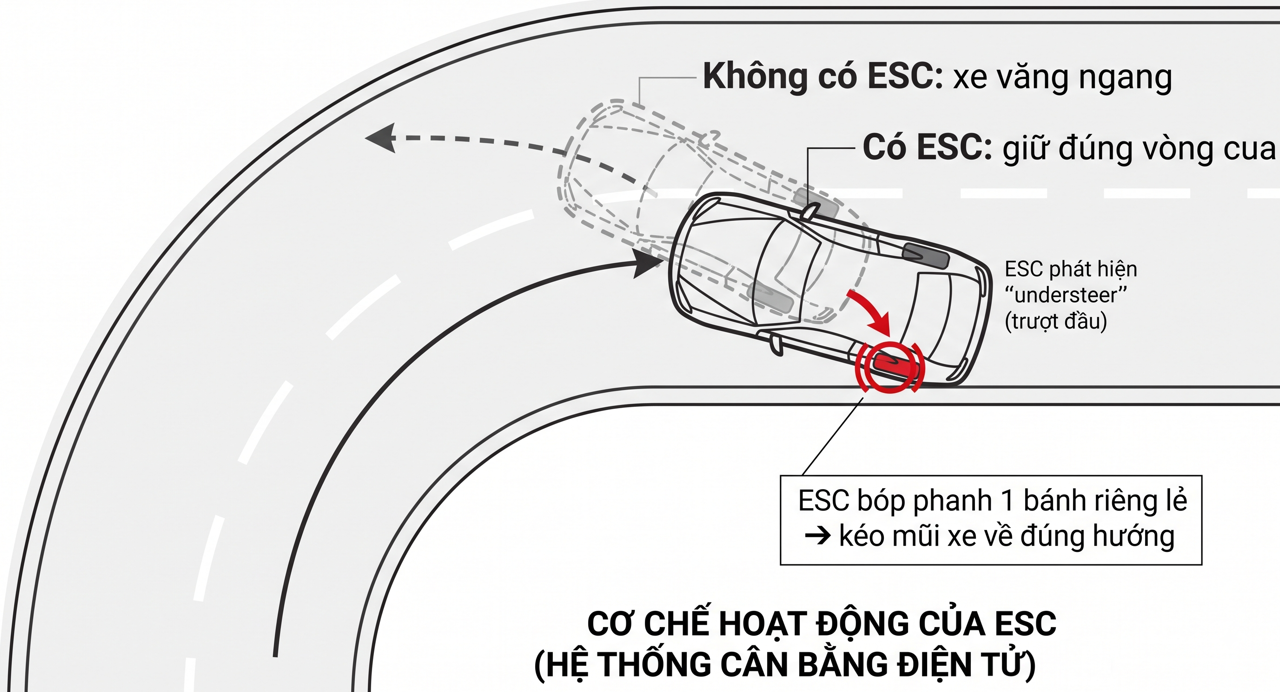
\includegraphics[width=0.7\textwidth]{image/abs_cd6_image3.png}
\end{center}
\figcaption{1}{Hệ thống cân bằng điện tử ESC giữ thân xe theo đúng vòng cua.}

\tablecaption{1}{So sánh chức năng của ABS và các hệ mở rộng.}
\setstretch{1.0}%
\begin{center}
\begin{tabular}{|>{\raggedright\arraybackslash}m{1.2cm}|>{\raggedright\arraybackslash}m{3.8cm}|>{\raggedright\arraybackslash}m{2cm}|>{\raggedright\arraybackslash}m{5.5cm}|}
\hline
\rowcolor{primaryBlue!12}
\textbf{Hệ thống} & \textbf{Nhiệm vụ} & \textbf{Dùng lại từ ABS} & \textbf{Điều khiển riêng lẻ từng bánh?} \\
\hline
ABS & Chống khóa bánh khi phanh gấp & (nền gốc) & Có (nhấp nhả phanh độc lập tại chính bánh đang có nguy cơ bị khóa) \\
\hline
CBS & Chia lực giữa hai bánh khi bóp một phanh & cụm van & Không (chỉ chia lực theo một tỉ lệ cố định cài sẵn) \\
\hline
EBD & Chia lực phanh trước sau theo tải & cảm biến + van & Có (phân bổ lực phanh khác nhau cho từng bánh tùy thuộc vào tải trọng thực tế) \\
\hline
ESC & Bóp từng bánh để chống văng khi vào cua & cảm biến + van & Có (chủ động phanh độc lập 1 hoặc 2 bánh bất kỳ để tạo lực xoay ngược lại) \\
\hline
\end{tabular}
\end{center}

Cả bốn hệ thống có tên gọi khác nhau nhưng phát triển từ cùng một nền tảng. Nắm được nguyên lý ABS giúp hiểu các hệ mở rộng, vì bản chất chỉ là trả lời câu hỏi ``cùng bộ cảm biến và van đó còn làm được gì''.

\hfill\textbf{Nguồn: Nguyễn Nghĩa Đô biên soạn}
\end{readingpassage}
\vspace{2pt}
\question[Trắc nghiệm]{Điểm chung về cấu tạo của các hệ thống CBS, EBD và ESC so với hệ thống gốc ABS là gì?}
\par\vspace{4pt}
\noindent\hangindent=2.2em\hangafter=1\choiceitem{A}{Tích hợp thêm cảm biến tốc độ mới chuyên biệt cho từng trục xe.}\par\vspace{4pt}
\noindent\hangindent=2.2em\hangafter=1\choiceitem{B}{Bổ sung hệ thống van điều biến độc lập để chống khóa bánh.}\par\vspace{4pt}
\noindent\hangindent=2.2em\hangafter=1\choiceitem{C}{Sử dụng lại chính cụm van hoặc/và cảm biến tốc độ nguyên bản.}\par\vspace{4pt}
\noindent\hangindent=2.2em\hangafter=1\choiceitem{D}{Yêu cầu bắt buộc đo đạc độ trượt của bánh xe ở mọi tình huống.}\par\vspace{4pt}

\question[Trắc nghiệm]{Hệ thống CBS phân biệt với EBD ở cơ chế cốt lõi nào khi thực hiện phân bổ lực phanh?}
\par\vspace{4pt}
\noindent\hangindent=2.2em\hangafter=1\choiceitem{A}{CBS chia lực giữa hai bánh khi bóp một phanh, trong khi EBD chia lực trước-sau theo tải.}\par\vspace{4pt}
\noindent\hangindent=2.2em\hangafter=1\choiceitem{B}{CBS sử dụng cả cảm biến và van của ABS, còn EBD chỉ dùng lại cụm van gốc.}\par\vspace{4pt}
\noindent\hangindent=2.2em\hangafter=1\choiceitem{C}{CBS đo độ trượt để chống khóa bánh, còn EBD bóp phanh từng bánh để chống văng.}\par\vspace{4pt}
\noindent\hangindent=2.2em\hangafter=1\choiceitem{D}{CBS chia đều lực phanh trước-sau, còn EBD phân bổ lực giữa hai bánh trên cùng một trục.}\par\vspace{4pt}

\question[Trắc nghiệm]{Theo dữ liệu từ Hình 1 và Bảng 1, hệ thống Cân bằng điện tử (ESC) nhận biết tình trạng văng ngang của xe thông qua yếu tố nào và xử lý ra sao?}
\par\vspace{4pt}
\noindent\hangindent=2.2em\hangafter=1\choiceitem{A}{Nhận biết qua việc người lái đạp phanh gấp và xử lý bằng cách chia đều lực cho các bánh.}\par\vspace{4pt}
\noindent\hangindent=2.2em\hangafter=1\choiceitem{B}{Nhận biết qua chênh lệch tốc độ các bánh và xử lý bằng cách bóp phanh một bánh riêng lẻ.}\par\vspace{4pt}
\noindent\hangindent=2.2em\hangafter=1\choiceitem{C}{Nhận biết qua tải trọng dồn về phía trước và xử lý bằng cách giảm lực phanh bánh sau.}\par\vspace{4pt}
\noindent\hangindent=2.2em\hangafter=1\choiceitem{D}{Nhận biết qua độ trượt của lốp và chia lực phanh cân bằng cho cả 4 lốp xe.}\par\vspace{4pt}

\question[Trắc nghiệm]{Giả định một chiếc xe thương mại có khối lượng tập trung 70\% ở nửa thân trước. Nếu chất thêm 500\,kg hàng hóa hoàn toàn vào cốp sau xe, hệ thống EBD sẽ lập mô hình phân phối lực phanh thay đổi như thế nào so với lúc xe chạy không tải?}
\par\vspace{4pt}
\noindent\hangindent=2.2em\hangafter=1\choiceitem{A}{Cố định tỷ lệ lực phanh chia đều 50:50 cho hai trục để ngăn thân xe bị văng ngang như CBS.}\par\vspace{4pt}
\noindent\hangindent=2.2em\hangafter=1\choiceitem{B}{Giảm lực phanh ở trục sau xuống mức tối thiểu vì bánh sau lúc này bị nhẹ tải.}\par\vspace{4pt}
\noindent\hangindent=2.2em\hangafter=1\choiceitem{C}{Tăng tỷ lệ lực phanh phân bổ về trục sau so với ban đầu để phù hợp với tải trọng tăng thêm.}\par\vspace{4pt}
\noindent\hangindent=2.2em\hangafter=1\choiceitem{D}{Kích hoạt bóp phanh một bánh riêng lẻ ở phía sau để ngăn bánh xe bị trượt cứng.}\par\vspace{4pt}

\question[Đúng/Sai]{Khi quan sát sơ đồ thiết kế linh kiện từ Bảng 1, một kỹ thuật viên đưa ra các nhận định sau, xác định Đúng/Sai:}

\vspace{6pt}
\renewcommand{\arraystretch}{1.4}
{\small\setstretch{1.0}
\begin{longtable}{|>{\raggedright\arraybackslash}m{0.72\textwidth}|>{\centering\arraybackslash}m{0.08\textwidth}|>{\centering\arraybackslash}m{0.08\textwidth}|}
\hline
\rowcolor{primaryBlue!12}
\textbf{Nội dung} & \textbf{Đúng} & \textbf{Sai} \\
\hline
\endfirsthead
\hline
\rowcolor{primaryBlue!12}
\textbf{Nội dung} & \textbf{Đúng} & \textbf{Sai} \\
\hline
\endhead
a) ABS cung cấp nền tảng vật lý cốt lõi bao gồm cụm van điều biến và cảm biến tốc độ. & \tfcircle & \tfcircle \\
\hline
b) Cả ba hệ thống CBS, EBD và ESC đều kế thừa hoàn toàn toàn bộ linh kiện của ABS. & \tfcircle & \tfcircle \\
\hline
c) Mọi hệ thống mở rộng đều sử dụng dữ liệu từ cảm biến tốc độ bánh xe của ABS. & \tfcircle & \tfcircle \\
\hline
d) Sự khác biệt chính của các hệ mở rộng so với ABS nằm ở thuật toán ra lệnh của bộ điều khiển. & \tfcircle & \tfcircle \\
\hline
\end{longtable}
}
\question[Đúng/Sai]{Một trung tâm kiểm định thử nghiệm hệ thống phanh trên đường sa hình. Dựa vào nguyên lý hoạt động (Hình 1, Bảng 1), đánh giá các chẩn đoán lỗi sau:}

\vspace{6pt}
\renewcommand{\arraystretch}{1.4}
{\small\setstretch{1.0}
\begin{longtable}{|>{\raggedright\arraybackslash}m{0.72\textwidth}|>{\centering\arraybackslash}m{0.08\textwidth}|>{\centering\arraybackslash}m{0.08\textwidth}|}
\hline
\rowcolor{primaryBlue!12}
\textbf{Nội dung} & \textbf{Đúng} & \textbf{Sai} \\
\hline
\endfirsthead
\hline
\rowcolor{primaryBlue!12}
\textbf{Nội dung} & \textbf{Đúng} & \textbf{Sai} \\
\hline
\endhead
a) Nếu bánh xe liên tục bị khóa cứng lê trên mặt đường khi phanh thẳng, lỗi chắc chắn nằm ở chức năng phân bổ tải của EBD. & \tfcircle & \tfcircle \\
\hline
b) Nếu xe bị văng đuôi khi cua gắt mà không hề đạp phanh, nguyên nhân có thể do ESC không bóp phanh kịp thời vào một lốp riêng lẻ. & \tfcircle & \tfcircle \\
\hline
c) Khi bóp một phanh tay mà xe máy bị văng đuôi, thợ máy cần thay mới bộ cảm biến đo độ trượt của hệ thống CBS. & \tfcircle & \tfcircle \\
\hline
d) Nếu bánh sau xe bị khóa sớm khi không chở hàng, lỗi xuất phát từ việc EBD không giảm lực phanh tương ứng cho trục sau vốn đang nhẹ tải. & \tfcircle & \tfcircle \\
\hline
\end{longtable}
}
\question[Điền khuyết]{Kết hợp bài đọc và Bảng 1, điền số (làm tròn đến phần đơn vị) và cụm từ thích hợp:}

\setstretch{1.4}
\begin{itemize}[leftmargin=*, itemsep=5pt, topsep=0pt, partopsep=0pt, parsep=0pt, label=\textcolor{primaryBlue}{\textbullet}]
\item Từ 1 hệ thống nền gốc là ABS, các kỹ sư đã thiết lập thêm (1)\,\dropbox[1.5cm] hệ thống phái sinh.
\item Khi xe vận hành, cơ chế đọc tải để bảo vệ bánh sau nhẹ tải thuộc nhiệm vụ của (2)\,\dropbox[2cm], trong khi đó, việc tự động giữ mũi xe đúng hướng bằng cách bóp một bánh riêng lẻ là nhiệm vụ của (3)\,\dropbox[2cm].
\end{itemize}
\question[Ghép đôi]{Ghép các hiện tượng hỏng hóc vật lý khi xe di chuyển (Cột A) với bộ phận có khả năng trục trặc trực tiếp cao nhất (Cột B).}

\vspace{6pt}
\setstretch{1.3}

\textit{Cột B:}
\vspace{-6pt}
\par\vspace{4pt}
\noindent\hangindent=2.2em\hangafter=1\choiceitem{A}{Hỏng chức năng liên kết thủy lực phân bổ giữa hai bánh của CBS.}\par\vspace{4pt}
\noindent\hangindent=2.2em\hangafter=1\choiceitem{B}{Cụm van chống bó cứng nguyên bản của ABS mất tác dụng.}\par\vspace{4pt}
\noindent\hangindent=2.2em\hangafter=1\choiceitem{C}{Lỗi thuật toán tính toán tải trọng trước-sau của hệ thống EBD.}\par\vspace{4pt}
\noindent\hangindent=2.2em\hangafter=1\choiceitem{D}{Bộ điều khiển bóp phanh độc lập từng bánh của hệ thống ESC bị liệt.}\par\vspace{4pt}

\vspace{6pt}

\renewcommand{\arraystretch}{1.6}
{\small\setstretch{1.0}
\begin{longtable}{|>{\raggedright\arraybackslash}m{0.55\textwidth}|>{\centering\arraybackslash}m{0.28\textwidth}|}
\hline
\rowcolor{primaryBlue!12}
\multicolumn{1}{|c|}{\cellcolor{primaryBlue!12}\textbf{Cột A}} & \cellcolor{primaryBlue!12}\textbf{Cột B} \\
\hline
\endfirsthead
\hline
\rowcolor{primaryBlue!12}
\multicolumn{1}{|c|}{\cellcolor{primaryBlue!12}\textbf{Cột A}} & \cellcolor{primaryBlue!12}\textbf{Cột B} \\
\hline
\endhead
1. Bánh xe trượt lê hoàn toàn trên mặt đường khi đạp chân phanh khẩn cấp. & \dropbox[2.5cm] \\
\hline
2. Bánh sau thường xuyên bị khóa bất thường dù xe không chở thêm hàng hóa. & \dropbox[2.5cm] \\
\hline
3. Khi cua gắt, mũi xe trôi ngang không hãm lại được dù bánh xe có sự chênh lệch tốc độ. & \dropbox[2.5cm] \\
\hline
4. Bóp tay phanh bên trái trên xe máy nhưng lực phanh không hề san sẻ sang bánh kia. & \dropbox[2.5cm] \\
\hline
\end{longtable}
}
\question[Ghép đôi]{Ghép yêu cầu ưu tiên an toàn khi vận hành (Cột A) với hệ thống sẽ đáp ứng chính xác nhất (Cột B).}

\vspace{6pt}
\setstretch{1.3}

\textit{Cột B:}
\vspace{-6pt}
\par\vspace{4pt}
\noindent\hangindent=2.2em\hangafter=1\choiceitem{A}{ABS}\par\vspace{4pt}
\noindent\hangindent=2.2em\hangafter=1\choiceitem{B}{CBS}\par\vspace{4pt}
\noindent\hangindent=2.2em\hangafter=1\choiceitem{C}{EBD}\par\vspace{4pt}
\noindent\hangindent=2.2em\hangafter=1\choiceitem{D}{ESC}\par\vspace{4pt}
\noindent\hangindent=2.2em\hangafter=1\choiceitem{E}{Hệ thống túi khí}\par\vspace{4pt}

\vspace{6pt}

\renewcommand{\arraystretch}{1.6}
{\small\setstretch{1.0}
\begin{longtable}{|>{\raggedright\arraybackslash}m{0.55\textwidth}|>{\centering\arraybackslash}m{0.28\textwidth}|}
\hline
\rowcolor{primaryBlue!12}
\multicolumn{1}{|c|}{\cellcolor{primaryBlue!12}\textbf{Cột A}} & \cellcolor{primaryBlue!12}\textbf{Cột B} \\
\hline
\endfirsthead
\hline
\rowcolor{primaryBlue!12}
\multicolumn{1}{|c|}{\cellcolor{primaryBlue!12}\textbf{Cột A}} & \cellcolor{primaryBlue!12}\textbf{Cột B} \\
\hline
\endhead
1. Ưu tiên độ bám đường khi khối lượng hàng hóa dao động lớn trên trục sau xe tải nhẹ. & \dropbox[2.5cm] \\
\hline
2. Ưu tiên chống văng xe chủ động trên đoạn đèo trơn trượt dù tài xế không chạm phanh. & \dropbox[2.5cm] \\
\hline
3. Ưu tiên ngăn chặn hiện tượng lốp xe đóng băng trượt thẳng tắp khi phanh nhồi. & \dropbox[2.5cm] \\
\hline
4. Ưu tiên phân phối lực cân đối đơn giản cho người lái mô tô bóp một bên phanh. & \dropbox[2.5cm] \\
\hline
\end{longtable}
}
\question[Kéo thả]{Kéo thả từ khóa để đối chiếu sự khác biệt giữa hai hệ thống EBD và CBS dựa trên Bảng 1:}
\vspace{-4pt}
\dragitems{
\centering
    \dragitem{tải} \dragitem{hai bánh} \dragitem{CBS}\\[1pt]
    \dragitem{EBD} \dragitem{trục sau} \dragitem{ESC} \dragitem{độ trượt}
}

\setstretch{1.4}
Dù cả hai đều có chức năng chia lực, sự khác biệt sinh ra từ nền tảng đầu vào. Hệ thống (1)\,\dropbox[2cm] không sử dụng cảm biến tốc độ nên không quan tâm đến việc đo lường bất cứ thứ gì, nó chỉ san sẻ lực giữa (2)\,\dropbox[2cm] cho cân. Ngược lại, hệ thống phân bổ lực phanh điện tử (3)\,\dropbox[2cm] lại bắt buộc theo dõi sự thay đổi về (4)\,\dropbox[1.5cm] trên các trục xe thông qua cảm biến nhằm tối ưu hóa phân bổ, ngăn lốp nhẹ bị trượt sớm.






% ============================================================
% CHỦ ĐỀ 7: PHANH TÁI SINH
% ============================================================
\newpage
\setcounter{qcounter}{0}

\phantomsection\label{b2_cd3_7}
\begin{topicbox}{\large CHỦ ĐỀ 7: PHANH TÁI SINH}
\vspace{8pt}
\textit{Đọc đoạn văn sau và trả lời các câu hỏi.}
\vspace{6pt}
\end{topicbox}

\begin{readingpassage}[]
\setstretch{1.3}

\textbf{Cơ chế chuyển hóa động năng}

Quá trình phanh xe máy điện yêu cầu giảm động năng của hệ (phương tiện và người lái) về xấp xỉ 0. Các hệ thống phanh khác nhau ở dạng năng lượng mà lượng động năng đó được chuyển đổi sang.

Với tổng khối lượng $m$ và vận tốc ban đầu $v_0$ ($v_0 > 0$), động năng cần triệt tiêu trong mỗi chu kỳ dừng là:
\[ E_k = \frac{1}{2}\,m\,v_0^2 \]

Với phanh ma sát, má phanh ép vào đĩa hoặc tang trống; lực ma sát chuyển đổi động năng thành nhiệt tỏa ra môi trường, gây tích tụ nhiệt trên cụm phanh sau nhiều lần vận hành liên tiếp.

Với phanh động cơ, khi nhả ga, động cơ tạo mô-men cản để giảm tốc. Năng lượng sinh ra chuyển thành nhiệt bên trong động cơ và không được lưu giữ.

Với phanh tái sinh, mô-tơ hoạt động như máy phát điện trong quá trình giảm tốc; quán tính bánh xe làm quay mô-tơ và phát sinh điện năng nạp ngược lại pin. Do tổn thất qua các cấp chuyển đổi, tỷ lệ thu hồi không đạt $100\%$; phần lực hãm còn lại do phanh ma sát đảm nhận.

\begin{center}
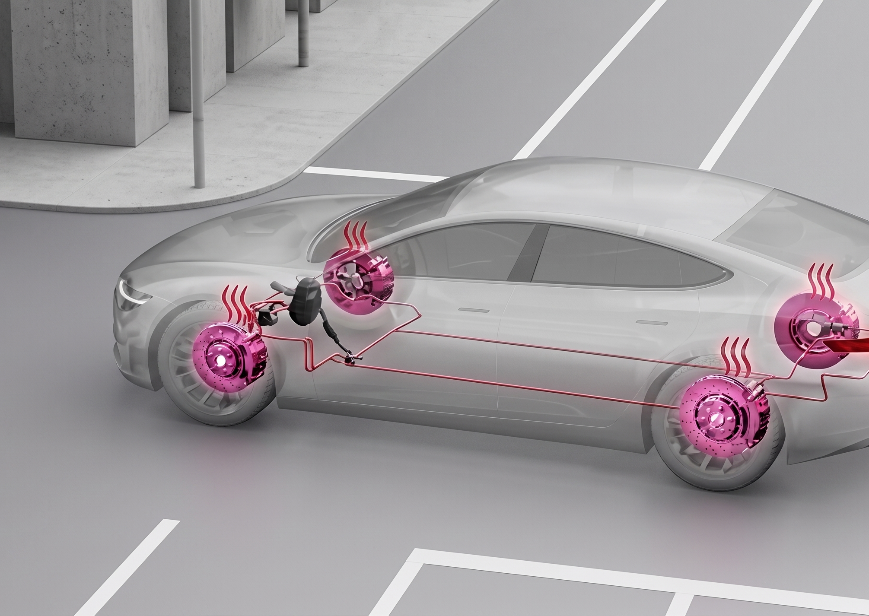
\includegraphics[width=0.65\textwidth]{image/abs_cd7_image1.png}
\end{center}
\figcaption{1}{Phanh ma sát dừng xe bằng chuyển động năng thành nhiệt năng và tiêu tán.}

\tablecaption{1}{So sánh đặc tính của ba phương thức phanh (cho một chu kỳ dừng).}
\renewcommand{\arraystretch}{1.4}
{\small
\begin{center}
\begin{tabular}{|>{\raggedright\arraybackslash}m{3.5cm}|>{\centering\arraybackslash}m{3cm}|>{\centering\arraybackslash}m{3cm}|>{\centering\arraybackslash}m{3cm}|}
\hline
\rowcolor{primaryBlue!12}
\textbf{Tiêu chí} & \textbf{Phanh ma sát} & \textbf{Phanh động cơ} & \textbf{Phanh tái sinh} \\
\hline
Dạng năng lượng chuyển đổi & Nhiệt tại má phanh & Nhiệt trong động cơ & Điện nạp vào pin \\
\hline
Hiệu suất thu hồi vào pin & $0\%$ & $0\%$ & $\approx 35\%$ \\
\hline
Mức độ mài mòn má phanh & Cao & Trung bình & Thấp \\
\hline
\end{tabular}
\end{center}
}

Bảng 1 cho thấy chỉ có phanh tái sinh thu hồi được một phần động năng thành điện năng. Lượng điện thu hồi ở mỗi lần phanh tuy nhỏ, nhưng khi tích lũy trong điều kiện đô thị với tần suất phanh cao sẽ tạo ra tổng năng lượng đáng kể.

\textbf{Cân bằng năng lượng tích lũy}

\tablecaption{2}{So sánh năng lượng sau 200 chu kỳ phanh ($m = 150$\,kg, giảm từ 36\,km/h về 0\,km/h).}
\renewcommand{\arraystretch}{1.4}
{\small
\begin{center}
\begin{tabular}{|>{\raggedright\arraybackslash}m{3cm}|>{\centering\arraybackslash}m{2.5cm}|>{\centering\arraybackslash}m{2.8cm}|>{\centering\arraybackslash}m{2.8cm}|}
\hline
\rowcolor{primaryBlue!12}
\textbf{Phương thức phanh} & \textbf{Tổng động năng} & \textbf{Nhiệt lượng tiêu tán} & \textbf{Điện năng thu hồi} \\
\hline
Phanh ma sát & $1\,500\,000$\,J & $1\,500\,000$\,J & $0$\,J \\
\hline
Phanh tái sinh & $1\,500\,000$\,J & $975\,000$\,J & $525\,000$\,J \\
\hline
\end{tabular}
\end{center}
}

Sau 200 chu kỳ dừng, tổng động năng cần xử lý ở cả hai phương thức đều bằng $1\,500\,000$\,J, nhưng phanh ma sát chuyển toàn bộ thành nhiệt tiêu tán, trong khi phanh tái sinh đưa $525\,000$\,J trở lại pin và chỉ tiêu tán $975\,000$\,J dưới dạng nhiệt.

\textbf{Nguyên lý điều khiển hệ thống phanh phối hợp}

Trong thực tế, phanh tái sinh và phanh ma sát hoạt động phối hợp đồng thời trong mỗi lần bóp phanh: bộ điều khiển liên tục tính toán tỷ lệ lực hãm giữa mô-tơ và má phanh theo vận tốc xe, dung lượng pin và lực phanh tác động, đảm bảo tổng lực hãm đáp ứng đúng yêu cầu của người điều khiển.

Ở vận tốc cao, mô-tơ đảm nhận phần lớn lực hãm để tối ưu hóa việc nạp điện. Khi vận tốc giảm dần, lực hãm từ mô-tơ suy giảm, má phanh tự động tăng lực ép để bù đắp sai lệch, duy trì quá trình giảm tốc liên tục.

Dải vận tốc dưới $5$--$10$\,km/h là vùng mù của hệ thống: rô-to quay chậm không đủ để tạo ra suất điện động cảm ứng hữu ích, lực hãm mô-tơ gần như triệt tiêu. Bộ điều khiển tự động chuyển toàn bộ lực hãm sang phanh ma sát để phương tiện dừng hẳn.

\hfill\textbf{Nguồn: Nguyễn Nghĩa Đô biên soạn}
\end{readingpassage}

% === Câu 1: Trắc nghiệm ===
\question[Trắc nghiệm]{Dựa vào Bảng 1, phương thức phanh nào gây mài mòn má phanh ở mức cao nhất và động năng trong phương thức đó được chuyển hóa thành dạng năng lượng gì?}
\par\vspace{4pt}
\noindent\hangindent=2.2em\hangafter=1\choiceitem{A}{Phanh ma sát, chuyển thành nhiệt lượng tiêu tán tại má phanh.}\par\vspace{4pt}
\noindent\hangindent=2.2em\hangafter=1\choiceitem{B}{Phanh tái sinh, chuyển thành điện năng nạp trực tiếp vào pin.}\par\vspace{4pt}
\noindent\hangindent=2.2em\hangafter=1\choiceitem{C}{Phanh động cơ, chuyển thành nhiệt năng lưu giữ trong động cơ.}\par\vspace{4pt}
\noindent\hangindent=2.2em\hangafter=1\choiceitem{D}{Phanh ma sát, chuyển thành động năng quay ngược của bánh xe.}\par\vspace{4pt}

% === Câu 2: Đúng/Sai ===
\question[Đúng/Sai]{Dựa vào Bảng 1 và Bảng 2, các phát biểu sau đây là đúng hay sai?}


\vspace{6pt}
\renewcommand{\arraystretch}{1.4}
{\small\setstretch{1.0}
\begin{longtable}{|>{\raggedright\arraybackslash}m{0.72\textwidth}|>{\centering\arraybackslash}m{0.08\textwidth}|>{\centering\arraybackslash}m{0.08\textwidth}|}
\hline
\rowcolor{primaryBlue!12}
\textbf{Nội dung} & \textbf{Đúng} & \textbf{Sai} \\
\hline
\endfirsthead
\hline
\rowcolor{primaryBlue!12}
\textbf{Nội dung} & \textbf{Đúng} & \textbf{Sai} \\
\hline
\endhead
a) Phanh động cơ và phanh ma sát có cùng mức hiệu suất thu hồi điện năng vào pin. & \tfcircle & \tfcircle \\
\hline
b) Phanh tái sinh có khả năng chuyển hóa $100\%$ động năng thành điện năng dự trữ. & \tfcircle & \tfcircle \\
\hline
c) Ở một chu kỳ dừng từ 36\,km/h về 0\,km/h với khối lượng 150\,kg, phanh tái sinh thu hồi được 525\,000\,J điện năng. & \tfcircle & \tfcircle \\
\hline
d) Mức độ mài mòn má phanh của ba phương thức tương quan nghịch với lượng nhiệt tiêu tán. & \tfcircle & \tfcircle \\
\hline
\end{longtable}
}

% === Câu 3: Ghép đôi ===
\question[Ghép đôi]{Ghép các thành phần và giai đoạn của hệ thống phanh với đặc điểm hoạt động tương ứng:}

\vspace{6pt}
\setstretch{1.3}

\textit{Cột B:}
\vspace{-6pt}
\par\vspace{4pt}
\noindent\hangindent=2.2em\hangafter=1\choiceitem{A}{Liên tục tính toán và phân bổ lực hãm phối hợp giữa mô-tơ và má phanh.}\par\vspace{4pt}
\noindent\hangindent=2.2em\hangafter=1\choiceitem{B}{Mô-tơ điện đảm nhận phần lớn lực hãm nhằm tối ưu hóa việc nạp điện.}\par\vspace{4pt}
\noindent\hangindent=2.2em\hangafter=1\choiceitem{C}{Mô-men cản sinh ra nhưng mọi năng lượng đều biến thành nhiệt tiêu tán.}\par\vspace{4pt}
\noindent\hangindent=2.2em\hangafter=1\choiceitem{D}{Rô-to quay quá chậm khiến mô-tơ gần như không tạo ra suất điện động hữu ích.}\par\vspace{4pt}

\vspace{6pt}

\renewcommand{\arraystretch}{1.6}
{\small\setstretch{1.0}
\begin{longtable}{|>{\raggedright\arraybackslash}m{0.55\textwidth}|>{\centering\arraybackslash}m{0.28\textwidth}|}
\hline
\rowcolor{primaryBlue!12}
\multicolumn{1}{|c|}{\cellcolor{primaryBlue!12}\textbf{Cột A}} & \cellcolor{primaryBlue!12}\textbf{Cột B} \\
\hline
\endfirsthead
\hline
\rowcolor{primaryBlue!12}
\multicolumn{1}{|c|}{\cellcolor{primaryBlue!12}\textbf{Cột A}} & \cellcolor{primaryBlue!12}\textbf{Cột B} \\
\hline
\endhead
1. Giai đoạn vận tốc cao & \dropbox[2.5cm] \\
\hline
2. Đặc tính vùng mù & \dropbox[2.5cm] \\
\hline
3. Phanh động cơ & \dropbox[2.5cm] \\
\hline
4. Bộ điều khiển trung tâm & \dropbox[2.5cm] \\
\hline
\end{longtable}
}

% === Câu 4: Điền khuyết ===
\question[Điền khuyết]{Một đoàn gồm 10 chiếc xe máy điện (mỗi xe nặng 150\,kg) cùng thực hiện phanh dừng trước đèn đỏ từ 36\,km/h. Hoàn thiện các mệnh đề sau:}
\vspace{2pt}
\setstretch{1.4}
Động năng cần xử lý của một xe trong lần dừng này là (1)\,\dropbox[2cm] J.
Nếu cả đoàn xe đều bị tắt hệ thống tái sinh và chỉ dùng phanh ma sát, mọi động năng này sẽ chuyển hóa thành (2)\,\dropbox[2cm] và tổng lượng tiêu tán ra môi trường của cả đoàn là (3)\,\dropbox[2cm] J.
Ngược lại, nếu dùng phanh tái sinh hoàn hảo, mỗi xe thu hồi được (4)\,\dropbox[2cm] J điện năng.

% === Câu 5: Điền khuyết đơn ===
\question[Điền khuyết]{Một chiếc xe điện (tổng khối lượng 200\,kg) thực hiện giảm tốc từ 54\,km/h xuống còn 18\,km/h. Lượng điện năng nạp vào pin trong giai đoạn này là bao nhiêu Jun? (Giả sử tỷ lệ thu hồi của phanh tái sinh luôn đạt mức lý thuyết 35\%).}

\vspace{4pt}
Kết quả: \dropbox[3cm]\,J.

% === Câu 6: Trắc nghiệm ===
\question[Trắc nghiệm]{Để tăng cường tổng lượng điện thu hồi ở điều kiện giao thông đô thị tắc nghẽn (xe chủ yếu chạy rề rà và liên tục phanh dừng từ tốc độ thấp), giải pháp kỹ thuật nào sau đây khắc phục trực tiếp nhất nhược điểm của phanh tái sinh được nêu trong bài?}
\par\vspace{4pt}
\noindent\hangindent=2.2em\hangafter=1\choiceitem{A}{Cải tiến phần cứng mô-tơ và thuật toán để thu hẹp dải ``vùng mù'' xuống dưới 3\,km/h.}\par\vspace{4pt}
\noindent\hangindent=2.2em\hangafter=1\choiceitem{B}{Sử dụng loại má phanh gốm chịu nhiệt tốt hơn để hãm hiệu quả ở tốc độ rất cao.}\par\vspace{4pt}
\noindent\hangindent=2.2em\hangafter=1\choiceitem{C}{Nâng cấp dung lượng pin để xe có thể chứa được tổng lượng điện lớn hơn trong một ngày.}\par\vspace{4pt}
\noindent\hangindent=2.2em\hangafter=1\choiceitem{D}{Tăng đường kính đĩa phanh ma sát để người lái dễ dàng dừng xe khi gặp vật cản.}\par\vspace{4pt}

% === Câu 7: Đúng/Sai ===
\question[Đúng/Sai]{Một hãng xe điện thử nghiệm phần mềm cho phép phanh tái sinh thu hồi cực đại lên tới $50\%$ động năng (giả định pin không bao giờ đầy). Các đánh giá sau về hệ thống phanh nâng cấp này là đúng hay sai?}


\vspace{6pt}
\renewcommand{\arraystretch}{1.4}
{\small\setstretch{1.0}
\begin{longtable}{|>{\raggedright\arraybackslash}m{0.72\textwidth}|>{\centering\arraybackslash}m{0.08\textwidth}|>{\centering\arraybackslash}m{0.08\textwidth}|}
\hline
\rowcolor{primaryBlue!12}
\textbf{Nội dung} & \textbf{Đúng} & \textbf{Sai} \\
\hline
\endfirsthead
\hline
\rowcolor{primaryBlue!12}
\textbf{Nội dung} & \textbf{Đúng} & \textbf{Sai} \\
\hline
\endhead
a) Khi xe bóp phanh từ 3\,km/h về đứng yên, lượng điện thu hồi sẽ đạt $50\%$ tổng động năng. & \tfcircle & \tfcircle \\
\hline
b) Ở dải tốc độ từ 40\,km/h xuống 10\,km/h, má phanh ma sát ít bị mòn hơn rất nhiều so với phần mềm cũ. & \tfcircle & \tfcircle \\
\hline
c) Khi pin đã sạc đầy $100\%$, xe vẫn phanh an toàn nhờ mô-tơ điện thu hồi $50\%$ lực vào pin. & \tfcircle & \tfcircle \\
\hline
d) Xe này có thể tháo bỏ hoàn toàn hệ thống phanh ma sát vì lực hãm $50\%$ từ mô-tơ đã đủ. & \tfcircle & \tfcircle \\
\hline
\end{longtable}
}

% === Câu 8: Kéo thả ===
\question[Kéo thả]{Kéo các cụm từ thích hợp vào chỗ trống để hoàn thành đoạn phân tích về thuật toán an toàn cho xe điện đi đường đèo:}
\vspace{-4pt}
\dragitems{
\centering
    \dragitem{quá nhiệt} \dragitem{sạc đầy} \dragitem{ngắt phanh tái sinh}\\[1pt]
    \dragitem{duy trì} \dragitem{vùng mù} \dragitem{tăng cao}\\[1pt]
    \dragitem{giảm xuống} \dragitem{cạn kiệt}
}

\setstretch{1.4}
Khi phát triển thuật toán an toàn cho xe điện đi đường đèo, bài toán cốt lõi là chống (1)\,\dropbox[2cm] cụm phanh. Khi xe đổ đèo và dung lượng pin chưa bão hòa, mô-tơ điện sẽ cung cấp lực hãm, giúp má phanh ma sát mát mẻ. Tuy nhiên, nếu đoạn đèo quá dài khiến pin bị (2)\,\dropbox[2cm] giữa chừng, bộ điều khiển bắt buộc phải (3)\,\dropbox[2cm] để bảo vệ tuổi thọ pin khỏi dòng nạp nhồi. Gánh nặng hãm xe lúc này dồn $100\%$ lên phanh ma sát, khiến nhiệt độ cụm phanh (4)\,\dropbox[2cm] cực nhanh và gây rủi ro mất phanh.

% === Câu 9: Ghép đôi ===
\question[Ghép đôi]{Phân tích các công nghệ hỗ trợ hệ thống phanh với nguyên lý kỹ thuật tương ứng:}

\vspace{6pt}
\setstretch{1.3}

\textit{Cột B:}
\vspace{-6pt}
\par\vspace{4pt}
\noindent\hangindent=2.2em\hangafter=1\choiceitem{A}{Hấp thụ dòng điện sạc khổng lồ sinh ra tức thời khi phanh gấp mà lõi pin hóa học không kịp nhận.}\par\vspace{4pt}
\noindent\hangindent=2.2em\hangafter=1\choiceitem{B}{Cá nhân hóa cảm giác ghì xe của người lái mỗi khi nhả chân ga (giả lập phanh động cơ).}\par\vspace{4pt}
\noindent\hangindent=2.2em\hangafter=1\choiceitem{C}{Đảm bảo năng lực dừng xe hoàn toàn và giữ độ bám đường khi mô-tơ mất lực hãm ở vùng mù.}\par\vspace{4pt}
\noindent\hangindent=2.2em\hangafter=1\choiceitem{D}{Ngăn ngừa tình trạng sạc nhồi gây cháy nổ khi pin đã chạm ngưỡng $100\%$ dung lượng.}\par\vspace{4pt}

\vspace{6pt}

\renewcommand{\arraystretch}{1.6}
{\small\setstretch{1.0}
\begin{longtable}{|>{\raggedright\arraybackslash}m{0.55\textwidth}|>{\centering\arraybackslash}m{0.28\textwidth}|}
\hline
\rowcolor{primaryBlue!12}
\multicolumn{1}{|c|}{\cellcolor{primaryBlue!12}\textbf{Cột A}} & \cellcolor{primaryBlue!12}\textbf{Cột B} \\
\hline
\endfirsthead
\hline
\rowcolor{primaryBlue!12}
\multicolumn{1}{|c|}{\cellcolor{primaryBlue!12}\textbf{Cột A}} & \cellcolor{primaryBlue!12}\textbf{Cột B} \\
\hline
\endhead
1. Lắp siêu tụ điện hấp thụ và xả năng lượng cực nhanh song song với pin. & \dropbox[2.5cm] \\
\hline
2. Thêm lẫy trên vô-lăng để người lái tự tùy chỉnh cường độ lực hãm của mô-tơ điện. & \dropbox[2.5cm] \\
\hline
3. Trang bị thêm cụm má phanh ma sát và đĩa phanh tiêu chuẩn ở bánh sau. & \dropbox[2.5cm] \\
\hline
4. Mạch điều khiển theo dõi điện áp, tự động ngắt dòng nạp ngược. & \dropbox[2.5cm] \\
\hline
\end{longtable}
}

% === Câu 10: Trắc nghiệm ===
\question[Trắc nghiệm]{Một xe đua Formula E có thể thu hồi tới $80\%$ động năng nhưng không trang bị phanh ma sát bánh sau để giảm trọng lượng. Điều gì chắc chắn xảy ra khi xe giảm từ 5\,km/h về đứng yên trong trạm pit-stop?}
\par\vspace{4pt}
\noindent\hangindent=2.2em\hangafter=1\choiceitem{A}{Xe dừng hoàn hảo nhờ khả năng thu hồi $80\%$ động năng.}\par\vspace{4pt}
\noindent\hangindent=2.2em\hangafter=1\choiceitem{B}{Động cơ tự đảo chiều quay để tạo nhiệt năng phanh xe.}\par\vspace{4pt}
\noindent\hangindent=2.2em\hangafter=1\choiceitem{C}{Xe rất khó dừng hẳn và có nguy cơ trôi vì mô-tơ mất lực hãm ở tốc độ thấp, trong khi không có phanh ma sát phụ trợ.}\par\vspace{4pt}
\noindent\hangindent=2.2em\hangafter=1\choiceitem{D}{Năng lượng nạp ngược từ pin ra làm bánh sau trượt lết.}\par\vspace{4pt}


% ============================================================
% CHỦ ĐỀ 8: CỤM TRUYỀN ĐỘNG VÀ INVERTER
% ============================================================
\newpage
\setcounter{qcounter}{0}

\phantomsection\label{b2_cd3_8}
\begin{topicbox}{\large CHỦ ĐỀ 8: CỤM TRUYỀN ĐỘNG VÀ INVERTER}
\vspace{8pt}
\textit{Đọc đoạn văn sau và trả lời các câu hỏi.}
\vspace{6pt}
\end{topicbox}

\begin{readingpassage}[]
\setstretch{1.3}

\textbf{Cấu trúc cụm truyền động}

Cụm truyền động của phương tiện thuần điện cấu thành từ ba phần tử liên kết mạch kín: bộ pin lưu trữ năng lượng điện một chiều (DC), bộ biến tần (inverter) thực hiện chuyển đổi định dạng dòng điện, và máy điện xoay chiều (mô-tơ AC) kết nối với trục bánh xe. Chế độ vận hành của phương tiện được xác định trực tiếp thông qua chiều dòng điện trong mạch: chế độ gia tốc xảy ra khi dòng điện truyền từ pin, qua inverter đến mô-tơ; khi dòng điện truyền ngược từ mô-tơ, qua inverter nạp về bộ pin, phương tiện đang thu hồi động năng thành điện năng, và cơ chế này chính là phanh tái sinh.

\begin{center}
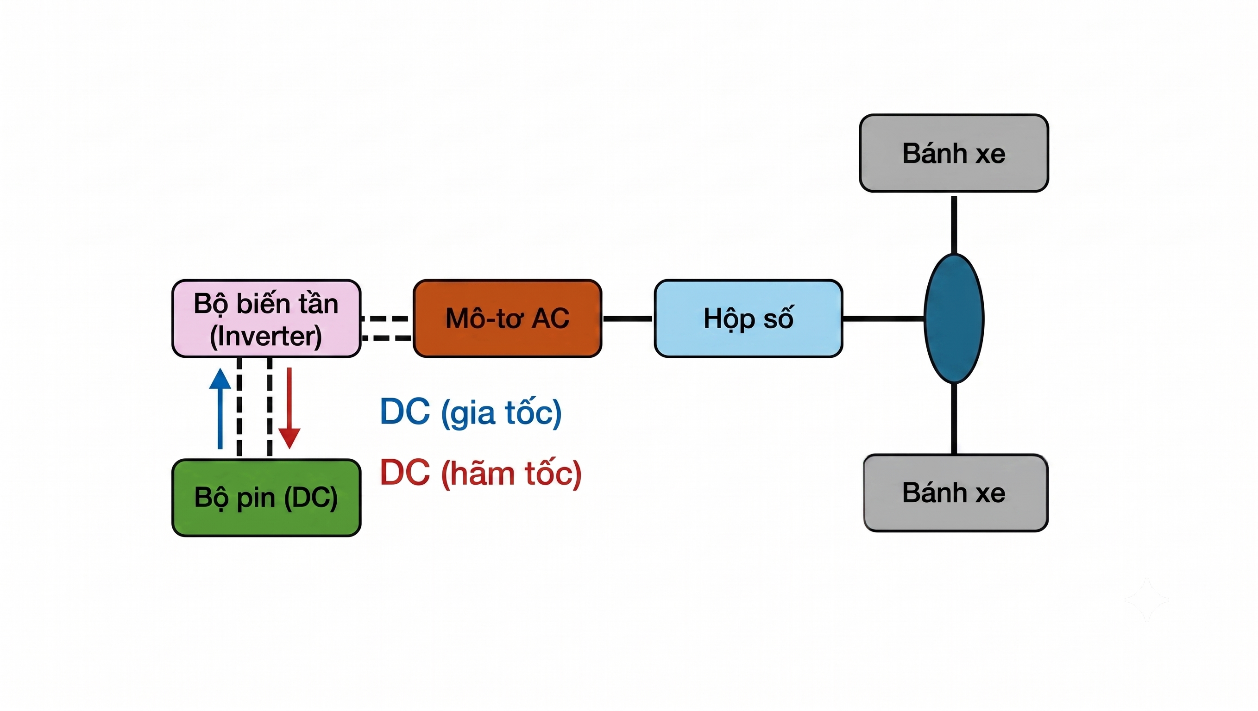
\includegraphics[width=0.65\textwidth]{image/abs_cd8_image1.png}
\end{center}
\figcaption{1}{Sơ đồ cụm truyền động xe điện.}

\textbf{Vai trò chuyển đổi kép của Inverter}

Linh kiện cốt lõi trong hệ thống là inverter, tức cầu nối bán dẫn công suất giữa pin và mô-tơ. Trong pha gia tốc, inverter đóng vai trò bộ nghịch lưu: biến đổi dòng DC từ pin thành dòng AC ba pha để cấp nguồn cho rô-tơ. Trong pha phanh tái sinh, động năng từ bánh xe dẫn động rô-tơ phát ra dòng AC; inverter lúc này chuyển sang vai trò bộ chỉnh lưu: nắn dòng AC thành DC để nạp ngược vào pin.

\tablecaption{1}{Trạng thái hoạt động của cụm Inverter -- Mô-tơ.}
\renewcommand{\arraystretch}{1.4}
{\small
\begin{center}
\begin{tabular}{|>{\raggedright\arraybackslash}m{2cm}|>{\centering\arraybackslash}m{1.8cm}|>{\centering\arraybackslash}m{2.8cm}|>{\centering\arraybackslash}m{1.5cm}|>{\centering\arraybackslash}m{1.8cm}|>{\raggedright\arraybackslash}m{3cm}|}
\hline
\rowcolor{primaryBlue!12}
\textbf{Thao tác} & \textbf{Inverter} & \textbf{Hiệu suất} & \textbf{Điện mô-tơ} & \textbf{Mô-tơ} & \textbf{Kết quả} \\
\hline
Gia tốc (Vặn ga) & Nghịch lưu & $\sim 90\%$ (điện $\to$ cơ) & Nhận AC & Động cơ kéo & Pin xả, bánh xe truyền động \\
\hline
Giảm tốc (Nhả ga/Phanh) & Chỉnh lưu & $\sim 85\%$ (cơ $\to$ điện $\to$ pin) & Phát AC & Máy phát hãm & Pin nạp, bánh xe chịu mô-men cản \\
\hline
\end{tabular}
\end{center}
}

\textbf{Phân tích hiệu suất và đặc tính mô-men cản}

Dữ liệu từ Bảng 1 cho thấy sự bất đối xứng: chế độ động cơ (điện $\to$ cơ) đạt hiệu suất chuyển đổi khoảng $90\%$, trong khi chế độ máy phát nạp pin (cơ $\to$ điện $\to$ pin) chỉ đạt mức $85\%$ do quá trình chỉnh lưu và đặc tính nạp điện hóa của bộ pin sinh thêm tổn hao. Do đó, lượng động năng giải phóng khi thực hiện phanh tái sinh luôn nhỏ hơn mức năng lượng tiêu hao cho quá trình gia tốc tương ứng, chưa xét đến các tổn hao cơ học trên chuỗi truyền động.

Bản chất của hiện tượng ``ghì'' phương tiện khi ngắt ga là do sự xuất hiện của mô-men cản điện từ. Lực cản này phát sinh khi hệ thống thu hồi động năng từ quán tính bánh xe để quay rô-tơ phát điện. Cường độ của lực cản này biến thiên theo vận tốc và biên độ dòng phát điện: lực hãm sẽ suy giảm khi vận tốc tiệm cận $0$, và bị triệt tiêu hoàn toàn khi dung lượng pin đạt ngưỡng tối đa (SoC $= 100\%$) do bộ điều khiển trung tâm chủ động ngắt mạch nạp nhằm bảo vệ pin.

\hfill\textbf{Nguồn: Nguyễn Nghĩa Đô biên soạn}
\end{readingpassage}

% === Câu 1: Trắc nghiệm ===
\question[Trắc nghiệm]{Người lái đang buông ga và tốc độ xe điện đang giảm dần, cường độ lực ghì tác dụng lên bánh xe sẽ thay đổi thế nào?}
\par\vspace{4pt}
\noindent\hangindent=2.2em\hangafter=1\choiceitem{A}{Tăng dần đến khi xe dừng hẳn.}\par\vspace{4pt}
\noindent\hangindent=2.2em\hangafter=1\choiceitem{B}{Giảm dần theo tốc độ.}\par\vspace{4pt}
\noindent\hangindent=2.2em\hangafter=1\choiceitem{C}{Duy trì mức cố định.}\par\vspace{4pt}
\noindent\hangindent=2.2em\hangafter=1\choiceitem{D}{Mất hoàn toàn ngay lập tức.}\par\vspace{4pt}

% === Câu 2: Trắc nghiệm (tính toán) ===
\question[Trắc nghiệm]{Xe máy điện có khối lượng 180\,kg tăng tốc từ 0 lên 36\,km/h (10\,m/s), rồi phanh tái sinh về 0. Biết $E_k = \frac{1}{2}mv^2$. Hiệu suất tăng tốc là $90\%$, hiệu suất phanh tái sinh là $85\%$. Lượng điện pin tiêu hao NET sau một lần tăng--phanh hoàn chỉnh là bao nhiêu J?}
\par\vspace{4pt}
\noindent\choiceitem{A}{2\,350\,J.}\hfill\choiceitem{B}{1\,000\,J.}\hfill\choiceitem{C}{7\,650\,J.}\hfill\choiceitem{D}{10\,000\,J.}

% === Câu 3: Trắc nghiệm ===
\question[Trắc nghiệm]{Pin cung cấp 1\,000\,W DC trong quá trình vặn ga. Công suất cơ học tối đa truyền tới bánh xe là xấp xỉ bao nhiêu W (bỏ qua tổn hao cơ học ngoài mô-tơ)?}
\par\vspace{4pt}
\noindent\choiceitem{A}{1\,000\,W.}\hfill\choiceitem{B}{900\,W.}\hfill\choiceitem{C}{850\,W.}\hfill\choiceitem{D}{1\,100\,W.}

% === Câu 4: Trắc nghiệm ===
\question[Trắc nghiệm]{Nhận định nào mô tả đúng bản chất hiệu suất bất đối xứng giữa hai chiều vận hành?}
\par\vspace{4pt}
\noindent\hangindent=2.2em\hangafter=1\choiceitem{A}{Tăng tốc hiệu quả hơn phanh tái sinh về năng lượng.}\par\vspace{4pt}
\noindent\hangindent=2.2em\hangafter=1\choiceitem{B}{Phanh tái sinh hiệu quả hơn vì tận dụng được động năng dư.}\par\vspace{4pt}
\noindent\hangindent=2.2em\hangafter=1\choiceitem{C}{Hai chiều đối xứng vì dùng cùng một khối inverter.}\par\vspace{4pt}
\noindent\hangindent=2.2em\hangafter=1\choiceitem{D}{Tăng tốc hao nhiều hơn vì dòng DC kém ổn định hơn AC.}\par\vspace{4pt}

% === Câu 5: Trắc nghiệm ===
\question[Trắc nghiệm]{Tổ hợp vai trò nào của inverter và mô-tơ là chính xác khi so sánh hai thao tác?}
\par\vspace{4pt}
\noindent\hangindent=2.2em\hangafter=1\choiceitem{A}{Bóp phanh: nghịch lưu + kéo bánh; Vặn ga: chỉnh lưu + hãm bánh.}\par\vspace{4pt}
\noindent\hangindent=2.2em\hangafter=1\choiceitem{B}{Bóp phanh: nghịch lưu + hãm bánh; Vặn ga: chỉnh lưu + kéo bánh.}\par\vspace{4pt}
\noindent\hangindent=2.2em\hangafter=1\choiceitem{C}{Bóp phanh: chỉnh lưu + máy phát hãm bánh; Vặn ga: nghịch lưu + động cơ kéo bánh.}\par\vspace{4pt}
\noindent\hangindent=2.2em\hangafter=1\choiceitem{D}{Bóp phanh: chỉnh lưu + kéo bánh; Vặn ga: nghịch lưu + hãm bánh.}\par\vspace{4pt}

% === Câu 6: Trắc nghiệm ===
\question[Trắc nghiệm]{Xe lao dốc dài, người lái buông ga hoàn toàn nhưng xe không hề có cảm giác ghì và tiếp tục trôi tự do. Nguyên nhân vật lý nào đúng nhất?}
\par\vspace{4pt}
\noindent\hangindent=2.2em\hangafter=1\choiceitem{A}{Mô-tơ AC đã cháy cuộn dây.}\par\vspace{4pt}
\noindent\hangindent=2.2em\hangafter=1\choiceitem{B}{Pin đã đầy nên bộ điều khiển cắt dòng nạp ngược.}\par\vspace{4pt}
\noindent\hangindent=2.2em\hangafter=1\choiceitem{C}{Inverter đang bị khóa ở trạng thái nghịch lưu.}\par\vspace{4pt}
\noindent\hangindent=2.2em\hangafter=1\choiceitem{D}{Bánh xe mất ma sát với mặt đường.}\par\vspace{4pt}

% === Câu 7: Trắc nghiệm ===
\question[Trắc nghiệm]{Năng lượng tiêu từ pin để tăng tốc lên 50\,km/h lớn hơn đáng kể so với điện thu về khi phanh từ 50\,km/h xuống 0. Cơ chế nào gây ra bất đối xứng này?}
\par\vspace{4pt}
\noindent\hangindent=2.2em\hangafter=1\choiceitem{A}{Dòng AC tiêu hao khi chạy qua lõi mô-tơ quay ngược.}\par\vspace{4pt}
\noindent\hangindent=2.2em\hangafter=1\choiceitem{B}{Bánh xe không đủ lực ma sát để làm quay mô-tơ ở tốc độ cao.}\par\vspace{4pt}
\noindent\hangindent=2.2em\hangafter=1\choiceitem{C}{Quá trình chỉnh lưu AC$\to$DC để nạp pin sinh ra thêm hao phí.}\par\vspace{4pt}
\noindent\hangindent=2.2em\hangafter=1\choiceitem{D}{Pin DC từ chối nhận nếu dòng AC vượt giới hạn.}\par\vspace{4pt}

% === Câu 8: Trắc nghiệm ===
\question[Trắc nghiệm]{Xe máy điện hết pin bị xe tải kéo bằng dây cáp, người lái không vặn ga. Hiện tượng nào xảy ra bên trong cụm truyền động?}
\par\vspace{4pt}
\noindent\hangindent=2.2em\hangafter=1\choiceitem{A}{Mô-tơ quay nhưng không phát điện vì không có tín hiệu vặn ga.}\par\vspace{4pt}
\noindent\hangindent=2.2em\hangafter=1\choiceitem{B}{Pin tiếp tục xả nốt phần điện cuối cùng.}\par\vspace{4pt}
\noindent\hangindent=2.2em\hangafter=1\choiceitem{C}{Bánh xe kéo mô-tơ sinh dòng AC, inverter chỉnh lưu thành DC và nạp lại pin.}\par\vspace{4pt}
\noindent\hangindent=2.2em\hangafter=1\choiceitem{D}{Inverter kích hoạt nghịch lưu để chống lại lực kéo.}\par\vspace{4pt}

% === Câu 9: Đúng/Sai ===
\question[Đúng/Sai]{Đánh giá các phát biểu về inverter trong cụm truyền động xe máy điện:}


\vspace{6pt}
\renewcommand{\arraystretch}{1.4}
{\small\setstretch{1.0}
\begin{longtable}{|>{\raggedright\arraybackslash}m{0.72\textwidth}|>{\centering\arraybackslash}m{0.08\textwidth}|>{\centering\arraybackslash}m{0.08\textwidth}|}
\hline
\rowcolor{primaryBlue!12}
\textbf{Nội dung} & \textbf{Đúng} & \textbf{Sai} \\
\hline
\endfirsthead
\hline
\rowcolor{primaryBlue!12}
\textbf{Nội dung} & \textbf{Đúng} & \textbf{Sai} \\
\hline
\endhead
a) Inverter cho phép dòng điện chạy theo cả hai chiều trong vòng kín. & \tfcircle & \tfcircle \\
\hline
b) Khi vặn ga tăng tốc, inverter nắn dòng AC thành DC. & \tfcircle & \tfcircle \\
\hline
c) Chuyển đổi giữa nghịch lưu và chỉnh lưu thực hiện bằng cách đảo tín hiệu điều khiển. & \tfcircle & \tfcircle \\
\hline
d) Chiều DC$\to$AC tạo ra nhiều tổn hao hơn chiều AC$\to$DC. & \tfcircle & \tfcircle \\
\hline
\end{longtable}
}

% === Câu 10: Đúng/Sai ===
\question[Đúng/Sai]{Phân tích cơ chế phanh tái sinh và cảm giác ghì xe:}


\vspace{6pt}
\renewcommand{\arraystretch}{1.4}
{\small\setstretch{1.0}
\begin{longtable}{|>{\raggedright\arraybackslash}m{0.72\textwidth}|>{\centering\arraybackslash}m{0.08\textwidth}|>{\centering\arraybackslash}m{0.08\textwidth}|}
\hline
\rowcolor{primaryBlue!12}
\textbf{Nội dung} & \textbf{Đúng} & \textbf{Sai} \\
\hline
\endfirsthead
\hline
\rowcolor{primaryBlue!12}
\textbf{Nội dung} & \textbf{Đúng} & \textbf{Sai} \\
\hline
\endhead
a) Cảm giác ghì sinh ra vì mô-tơ lấy động năng từ bánh xe để phát điện. & \tfcircle & \tfcircle \\
\hline
b) Năng lượng tăng tốc luôn thu lại hoàn toàn khi phanh tái sinh. & \tfcircle & \tfcircle \\
\hline
c) Tốc độ xe càng thấp thì dòng phát điện càng nhỏ, cảm giác ghì càng yếu. & \tfcircle & \tfcircle \\
\hline
d) Khi pin gần đầy, bộ điều khiển tăng dòng nạp để tận dụng nốt động năng còn lại. & \tfcircle & \tfcircle \\
\hline
\end{longtable}
}


% ============================================================
% CHỦ ĐỀ 9: NHIỆT ĐỘ TRONG PHANH TÁI SINH
% ============================================================
\newpage
\setcounter{qcounter}{0}

\phantomsection\label{b2_cd3_9}
\begin{topicbox}{\large CHỦ ĐỀ 9: NHIỆT ĐỘ TRONG PHANH TÁI SINH}
\vspace{8pt}
\textit{Đọc đoạn văn sau và trả lời các câu hỏi.}
\vspace{6pt}
\end{topicbox}

\begin{readingpassage}[]
\setstretch{1.3}

Phanh tái sinh là quá trình mô-tơ điện đảo chiều hoạt động thành máy phát, chuyển hóa động năng của phương tiện thành điện năng để nạp ngược vào bộ pin. Ở điều kiện nhiệt độ vận hành bình thường, tổng hiệu suất của chu trình chuyển đổi này đạt khoảng $77\%$.

Trong quá trình nạp, pin Lithium-ion liên tục sinh nhiệt. Ở dải nhiệt độ thấp, các phản ứng điện hóa diễn ra ổn định với sự di chuyển đều đặn của ion lithium vào cấu trúc điện cực. Khi nhiệt độ vượt quá giới hạn an toàn, tốc độ phản ứng gia tăng mất kiểm soát, kéo theo nguy cơ biến dạng điện cực và đoản mạch nội bộ. Nhằm bảo vệ hệ thống, bộ quản lý pin (BMS) tự động can thiệp giới hạn dòng nạp thu hồi dựa trên hai mức giới hạn nhiệt độ thực tế. Sự suy giảm năng lượng thu hồi về mức 0 sau nhiều chu kỳ phanh liên tiếp chính là kết quả của cơ chế can thiệp bảo vệ nhiệt này.

Theo công bố của nhà sản xuất, đường đặc tính lý thuyết (Hình 1) thể hiện cơ chế can thiệp của BMS được chia thành ba vùng rõ rệt: vùng hiệu suất duy trì ổn định, vùng suy giảm tuyến tính khi chạm ngưỡng nhiệt độ cảnh báo, và vùng ngắt nạp hoàn toàn để bảo đảm an toàn.

\begin{center}
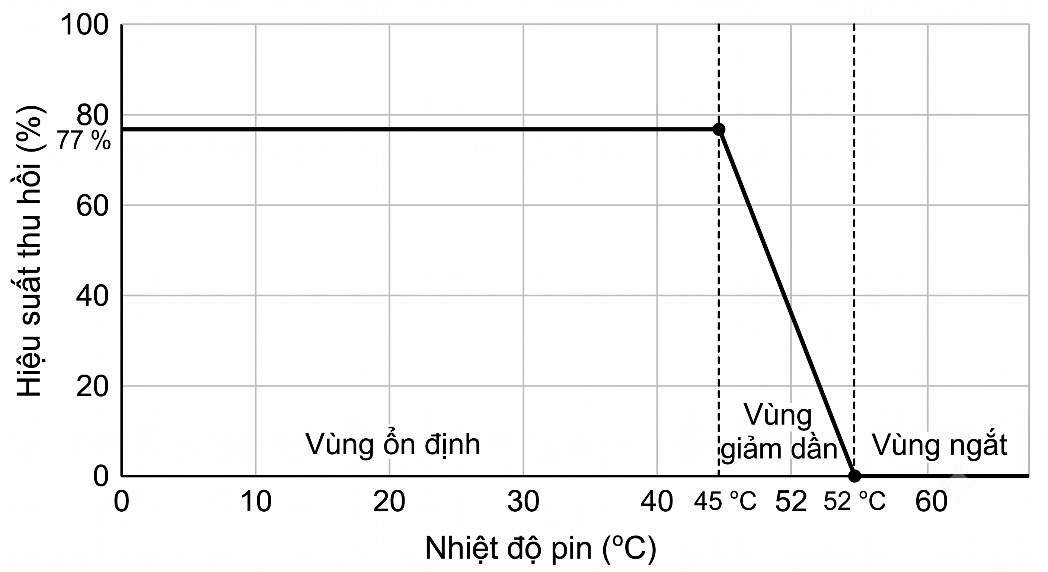
\includegraphics[width=0.6\textwidth]{image/abs_cd9_image1.png}
\end{center}
\figcaption{1}{Hiệu suất thu hồi lý thuyết theo nhiệt độ pin theo công bố của nhà sản xuất.}

Để kiểm tra cơ chế can thiệp của BMS, một thực nghiệm được thiết lập với phương tiện có khối lượng 1\,400\,kg, thực hiện giảm tốc từ 72\,km/h về 0 trên quãng đường nằm ngang cố định 80\,m. Động năng ban đầu của phương tiện được xác định theo phương trình $E_k = \frac{1}{2}mv^2$. Biến độc lập là nhiệt độ pin tại thời điểm bắt đầu mỗi lượt chạy được điều tiết chủ động thông qua hệ thống làm mát. Cảm biến được sử dụng để ghi nhận điện năng nạp vào pin sau từng lượt thử nghiệm.

\tablecaption{1}{Kết quả đo thực nghiệm.}
\renewcommand{\arraystretch}{1.4}
{\small
\begin{center}
\begin{tabular}{|>{\centering\arraybackslash}m{1.2cm}|>{\centering\arraybackslash}m{3.5cm}|>{\centering\arraybackslash}m{3.5cm}|>{\centering\arraybackslash}m{3cm}|}
\hline
\rowcolor{primaryBlue!12}
\textbf{Lượt} & \textbf{Nhiệt độ pin đầu lượt (\textdegree C)} & \textbf{Năng lượng thu hồi (kJ)} & \textbf{Hiệu suất thực đo (\%)} \\
\hline
1 & 22 & 216 & 77 \\
\hline
2 & 31 & 216 & 77 \\
\hline
3 & 40 & 216 & 77 \\
\hline
4 & 47 & 129 & 46 \\
\hline
5 & 54 & 0 & 0 \\
\hline
\end{tabular}
\end{center}
}

\hfill\textbf{Nguồn: Nguyễn Nghĩa Đô biên soạn}
\end{readingpassage}

% === Câu 1: Trắc nghiệm ===
\question[Trắc nghiệm]{Trong thiết kế thực nghiệm kiểm tra cơ chế can thiệp của BMS, biến độc lập được xác định là đại lượng nào?}
\par\vspace{4pt}
\noindent\hangindent=2.2em\hangafter=1\choiceitem{A}{Điện năng nạp lại vào bộ pin.}\par\vspace{4pt}
\noindent\hangindent=2.2em\hangafter=1\choiceitem{B}{Nhiệt độ pin ở đầu mỗi lượt chạy.}\par\vspace{4pt}
\noindent\hangindent=2.2em\hangafter=1\choiceitem{C}{Quãng đường phương tiện giảm tốc.}\par\vspace{4pt}
\noindent\hangindent=2.2em\hangafter=1\choiceitem{D}{Động năng ban đầu của chiếc xe.}\par\vspace{4pt}

% === Câu 2: Trắc nghiệm ===
\question[Trắc nghiệm]{Nguy cơ vật lý chính nào xảy ra bên trong cấu trúc pin khi nhiệt độ vận hành vượt quá giới hạn an toàn?}
\par\vspace{4pt}
\noindent\hangindent=2.2em\hangafter=1\choiceitem{A}{Đoản mạch nội bộ kéo theo tốc độ phản ứng gia tăng.}\par\vspace{4pt}
\noindent\hangindent=2.2em\hangafter=1\choiceitem{B}{Lõi mô-tơ điện bị kẹt do đảo chiều hoạt động.}\par\vspace{4pt}
\noindent\hangindent=2.2em\hangafter=1\choiceitem{C}{Động năng phương tiện chuyển hóa ngược thành nhiệt năng.}\par\vspace{4pt}
\noindent\hangindent=2.2em\hangafter=1\choiceitem{D}{Hệ thống làm mát quá tải gây rò rỉ dung môi.}\par\vspace{4pt}

% === Câu 3: Đúng/Sai ===
\question[Đúng/Sai]{Đánh giá tính chuẩn xác của các phát biểu sau về thiết kế và kết quả thí nghiệm:}


\vspace{6pt}
\renewcommand{\arraystretch}{1.4}
{\small\setstretch{1.0}
\begin{longtable}{|>{\raggedright\arraybackslash}m{0.72\textwidth}|>{\centering\arraybackslash}m{0.08\textwidth}|>{\centering\arraybackslash}m{0.08\textwidth}|}
\hline
\rowcolor{primaryBlue!12}
\textbf{Nội dung} & \textbf{Đúng} & \textbf{Sai} \\
\hline
\endfirsthead
\hline
\rowcolor{primaryBlue!12}
\textbf{Nội dung} & \textbf{Đúng} & \textbf{Sai} \\
\hline
\endhead
a) Cơ chế bảo vệ nhiệt của BMS khiến năng lượng thu hồi có thể suy giảm về mức 0. & \tfcircle & \tfcircle \\
\hline
b) Vùng ngắt nạp hoàn toàn theo lý thuyết bắt đầu khi pin chạm ngưỡng 45\textdegree C. & \tfcircle & \tfcircle \\
\hline
c) Ở lượt chạy số 2 và 3, hiệu suất thu hồi thực đo đạt mức tối đa. & \tfcircle & \tfcircle \\
\hline
d) Quá trình phanh tái sinh chuyển hóa điện năng thành động năng phương tiện. & \tfcircle & \tfcircle \\
\hline
\end{longtable}
}

% === Câu 4: Trắc nghiệm ===
\question[Trắc nghiệm]{Động năng ban đầu của phương tiện trước khi thực hiện mỗi lượt giảm tốc trong thực nghiệm có giá trị bằng bao nhiêu?}
\par\vspace{4pt}
\noindent\choiceitem{A}{280\,kJ.}\hfill\choiceitem{B}{3\,628\,kJ.}\hfill\choiceitem{C}{140\,kJ.}\hfill\choiceitem{D}{216\,kJ.}

% === Câu 5: Trắc nghiệm ===
\question[Trắc nghiệm]{Xác định mức hiệu suất thu hồi lý thuyết khi hệ thống pin vận hành ở nhiệt độ 50\textdegree C.}
\par\vspace{4pt}
\noindent\choiceitem{A}{$44\%$.}\hfill\choiceitem{B}{$33\%$.}\hfill\choiceitem{C}{$28\%$.}\hfill\choiceitem{D}{$22\%$.}

% === Câu 6: Trắc nghiệm ===
\question[Trắc nghiệm]{Mục đích kỹ thuật của việc điều tiết nhiệt độ qua hệ thống làm mát ngay trước mỗi lượt chạy là gì?}
\par\vspace{4pt}
\noindent\hangindent=2.2em\hangafter=1\choiceitem{A}{Mô phỏng luồng gió tự nhiên tản nhiệt cho xe khi di chuyển tốc độ cao.}\par\vspace{4pt}
\noindent\hangindent=2.2em\hangafter=1\choiceitem{B}{Thiết lập trạng thái nền chuẩn xác để khảo sát tác động độc lập của nhiệt.}\par\vspace{4pt}
\noindent\hangindent=2.2em\hangafter=1\choiceitem{C}{Triệt tiêu hoàn toàn lượng nhiệt sinh ra trong suốt thời gian xe giảm tốc.}\par\vspace{4pt}
\noindent\hangindent=2.2em\hangafter=1\choiceitem{D}{Kích thích sự di chuyển đều đặn của ion lithium vào cấu trúc điện cực.}\par\vspace{4pt}

% === Câu 7: Trắc nghiệm ===
\question[Trắc nghiệm]{Tính toán mức chênh lệch giữa năng lượng thu hồi theo lý thuyết và giá trị thực đo tại lượt chạy tiến hành ở 47\textdegree C.}
\par\vspace{4pt}
\noindent\choiceitem{A}{13\,kJ.}\hfill\choiceitem{B}{25\,kJ.}\hfill\choiceitem{C}{42\,kJ.}\hfill\choiceitem{D}{87\,kJ.}

% === Câu 8: Trắc nghiệm ===
\question[Trắc nghiệm]{Đâu là giả thuyết khoa học hợp lý nhất giải thích sự sụt giảm hiệu suất thực tế ($46\%$) so với lý thuyết ($55\%$) tại mốc 47\textdegree C?}
\par\vspace{4pt}
\noindent\hangindent=2.2em\hangafter=1\choiceitem{A}{Khối lượng 1\,400\,kg của phương tiện vượt quá giới hạn thiết kế của mô-tơ điện.}\par\vspace{4pt}
\noindent\hangindent=2.2em\hangafter=1\choiceitem{B}{Động năng xe bị tiêu hao một phần do lực cản khí động học trên quãng đường 80\,m.}\par\vspace{4pt}
\noindent\hangindent=2.2em\hangafter=1\choiceitem{C}{Nhiệt lượng sinh ra trong quá trình nạp làm nhiệt độ nội tại tiếp tục tăng vượt mốc 47\textdegree C.}\par\vspace{4pt}
\noindent\hangindent=2.2em\hangafter=1\choiceitem{D}{Biến dạng điện cực đã xảy ra hoàn toàn khiến chu trình chuyển đổi bị đứt gãy.}\par\vspace{4pt}

% === Câu 9: Trắc nghiệm ===
\question[Trắc nghiệm]{Một phương tiện (1\,400\,kg) đang vận hành với pin ở mức 48,5\textdegree C thì gặp chướng ngại vật, phải phanh giảm tốc từ 90\,km/h xuống còn 36\,km/h. Bỏ qua sự tăng nhiệt tức thời, điện năng lý thuyết được nạp lại trong pha xử lý này là bao nhiêu?}
\par\vspace{4pt}
\noindent\choiceitem{A}{141,5\,kJ.}\hfill\choiceitem{B}{283,0\,kJ.}\hfill\choiceitem{C}{367,5\,kJ.}\hfill\choiceitem{D}{477,7\,kJ.}

% === Câu 10: Trắc nghiệm ===
\question[Trắc nghiệm]{Thông qua một bản cập nhật phần mềm, ngưỡng ngắt nạp hoàn toàn được nới lỏng lên mức 55,5\textdegree C. Giữ nguyên độ dốc suy giảm tuyến tính lý thuyết, hãy xác định ngưỡng nhiệt độ cảnh báo mới và hiệu suất thu hồi khi pin đạt 51\textdegree C.}
\par\vspace{4pt}
\noindent\hangindent=2.2em\hangafter=1\choiceitem{A}{Ngưỡng mới: 47,5\textdegree C; Hiệu suất: $44{,}0\%$.}\par\vspace{4pt}
\noindent\hangindent=2.2em\hangafter=1\choiceitem{B}{Ngưỡng mới: 48,5\textdegree C; Hiệu suất: $49{,}5\%$.}\par\vspace{4pt}
\noindent\hangindent=2.2em\hangafter=1\choiceitem{C}{Ngưỡng mới: 48,5\textdegree C; Hiệu suất: $55{,}0\%$.}\par\vspace{4pt}
\noindent\hangindent=2.2em\hangafter=1\choiceitem{D}{Ngưỡng mới: 49,0\textdegree C; Hiệu suất: $60{,}5\%$.}\par\vspace{4pt}




% ============================================================
% CHỦ ĐỀ 10: CHẨN ĐOÁN VÀ PHÂN LOẠI HÀNH VI PHANH TÁI SINH
% ============================================================
\newpage
\setcounter{qcounter}{0}

\phantomsection\label{b2_cd3_10}
\begin{topicbox}{\large CHỦ ĐỀ 10: CHẨN ĐOÁN VÀ PHÂN LOẠI HÀNH VI PHANH TÁI SINH}
\vspace{8pt}
\textit{Đọc đoạn văn sau và trả lời các câu hỏi.}
\vspace{6pt}
\end{topicbox}

\begin{readingpassage}[]
\setstretch{1.3}

Trong cùng phân khúc xe máy điện, một số dòng được trang bị hệ thống phanh tái sinh trong khi các dòng khác chỉ sử dụng phanh ma sát cơ học truyền thống. Để phân loại, kỹ thuật viên cần nhận biết sự hiện diện của hệ thống này thông qua quan sát hành vi vận hành thực tế mà không dựa vào thiết bị đo chuyên dụng hay dữ liệu thiết kế nội bộ.

Quá trình khảo sát được tiến hành trên ba mẫu xe (ký hiệu X, Y, Z) có cùng khối lượng và thiết kế tương đương, không rõ thông số nội bộ. Bốn phép thử (T1--T4) được thiết kế nhằm đánh giá các biểu hiện vật lý và điện học đặc trưng mà không can thiệp vào kết cấu. Phép thử T1 (thả ga trên dốc 5\textdegree{}) nhằm quan sát trạng thái trôi tự do hoặc bị ghì lại do lực cản. T2 yêu cầu phanh lặp lại 20 lần từ 40\,km/h về 0 để đánh giá mức độ sinh nhiệt thực tế của má phanh. Hai phép thử còn lại theo dõi phản hồi điện và cơ: T3 ghi nhận sự biến thiên trên chỉ báo đồng hồ pin khi người lái thực hiện thao tác hãm, T4 khảo sát phản hồi của xe khi phanh ở dải tốc độ cực thấp (dưới 5\,km/h).

\tablecaption{1}{Kết quả quan sát hành vi phanh trên ba mẫu xe.}
\vspace{2pt}
\renewcommand{\arraystretch}{1.35}
{\small
\begin{center}
\begin{tabular}{|>{\centering\arraybackslash}m{0.8cm}|>{\centering\arraybackslash}m{2.8cm}|>{\centering\arraybackslash}m{2.2cm}|>{\centering\arraybackslash}m{3cm}|>{\centering\arraybackslash}m{2.2cm}|}
\hline
\rowcolor{primaryBlue!12}
\textbf{Xe} & \textbf{T1: Thả ga dốc} & \textbf{T2: Má phanh} & \textbf{T3: Đồng hồ pin} & \textbf{T4: < 5 km/h} \\
\hline
X & Trôi tự do, không ghì & Rất nóng & Giảm liên tục & Không ghì \\
\hline
Y & Ghì nhẹ, xe chậm dần rõ & Ấm & Tăng nhẹ khi đang phanh & Không ghì \\
\hline
Z & Ghì mạnh, giảm tốc nhanh & Mát & Tăng rõ khi đang phanh & Không ghì \\
\hline
\end{tabular}
\end{center}
}

\vspace{6pt}
Đối với xe có trang bị hệ thống phanh tái sinh, khi người lái buông ga hoặc bóp phanh, động năng của phương tiện được chuyển hóa thành điện năng thông qua việc biến mô-tơ điện thành một máy phát. Quá trình này sinh ra dòng điện nạp ngược trở lại hệ thống lưu trữ, đồng thời tạo ra mô-men cản điện từ tác động trực tiếp lên trục động cơ và tạo ra cảm giác ``ghì'' rất rõ rệt. Nhờ mô-men cản điện từ này gánh chịu phần lớn công trượt để làm chậm xe, hệ thống má phanh ma sát ít phải chịu tải hơn, dẫn đến nhiệt độ tỏa ra trên bề mặt giảm đáng kể, thường duy trì ở mức mát hoặc chỉ ấm nhẹ. Hiệu ứng điện từ này không diễn ra ở mọi dải tốc độ: trong phép thử tốc độ thấp, rô-to của động cơ quay quá chậm khiến từ thông biến thiên yếu, không đủ để sinh ra suất điện động hữu ích. Mô-men cản điện từ vì thế triệt tiêu, khiến xe rơi vào ``vùng mù'' của công nghệ và hoàn toàn mất cảm giác ghì, tương tự hành vi của một xe cơ học thuần túy.

Mặc dù các phép thử mang lại những dấu hiệu nhận diện trực quan, phương pháp này vẫn tồn tại giới hạn nhất định và dễ cho kết quả sai lệch trong các điều kiện phi tiêu chuẩn. Nếu chiếc xe có trang bị phanh tái sinh được đem thử nghiệm ngay lúc dung lượng pin đạt mức $100\%$ (SoC $100\%$), bộ điều khiển trung tâm sẽ tự động ngắt mạch nạp nhằm bảo vệ pin khỏi quá tải. Khi đó, động năng không thể xả thành dòng sạc, kéo theo việc mất hoàn toàn lực ghì ở T1 và chỉ báo pin ở T3 không thể tăng thêm, khiến kỹ thuật viên dễ chẩn đoán nhầm đó là mẫu xe không được trang bị hệ thống tái sinh. Nếu độ dốc ở phép thử T1 quá nhẹ, lực cản sinh ra cũng không đủ lớn để nhận diện sự khác biệt giữa các xe.

\hfill\textbf{Nguồn: Nguyễn Nghĩa Đô biên soạn}
\end{readingpassage}

% === Câu 1: Trắc nghiệm ===
\question[Trắc nghiệm]{Dựa vào bảng dữ liệu, ở phép thử T1, hiện tượng nào đã được quan sát thấy trên mẫu xe X?}
\par\vspace{4pt}
\noindent\hangindent=2.2em\hangafter=1\choiceitem{A}{Ghì nhẹ, xe chậm dần rõ.}\par\vspace{4pt}
\noindent\hangindent=2.2em\hangafter=1\choiceitem{B}{Xe dừng lại ngay lập tức.}\par\vspace{4pt}
\noindent\hangindent=2.2em\hangafter=1\choiceitem{C}{Trôi tự do, không ghì.}\par\vspace{4pt}
\noindent\hangindent=2.2em\hangafter=1\choiceitem{D}{Ghì mạnh, giảm tốc nhanh.}\par\vspace{4pt}

% === Câu 2: Trắc nghiệm ===
\question[Trắc nghiệm]{Tại phép thử T2, một mẫu xe có nhiệt độ má phanh thấp hơn đáng kể so với hai mẫu còn lại sau 20 lần phanh gấp. Nguyên nhân trực tiếp nào sau đây giải thích tốt nhất hiện tượng này?}
\par\vspace{4pt}
\noindent\hangindent=2.2em\hangafter=1\choiceitem{A}{Hệ thống tản nhiệt bằng chất lỏng của mẫu xe đó hoạt động hiệu quả hơn.}\par\vspace{4pt}
\noindent\hangindent=2.2em\hangafter=1\choiceitem{B}{Mẫu xe đó không sử dụng phanh ma sát ở dải tốc độ trên 40\,km/h.}\par\vspace{4pt}
\noindent\hangindent=2.2em\hangafter=1\choiceitem{C}{Mô-men cản điện từ đã gánh chịu phần lớn lực hãm thay cho má phanh.}\par\vspace{4pt}
\noindent\hangindent=2.2em\hangafter=1\choiceitem{D}{Má phanh của mẫu xe đó được chế tạo từ vật liệu có hệ số ma sát thấp hơn, sinh ít nhiệt hơn khi cùng lực ép.}\par\vspace{4pt}

% === Câu 3: Trắc nghiệm ===
\question[Trắc nghiệm]{Kỹ thuật viên thực hiện phép thử T1 và T3 trên mẫu xe K và ghi nhận: T1 -- cảm giác ghì rõ khi thả ga trên dốc 5\textdegree{}; T3 -- số chỉ đồng hồ pin tăng trong quá trình phanh. Trước lần thử tiếp theo, xe K được sạc đầy pin tới mức SoC = $100\%$. Kết quả T1 và T3 trong lần thử tiếp theo có khả năng cao nhất là gì?}
\par\vspace{4pt}
\noindent\hangindent=2.2em\hangafter=1\choiceitem{A}{T1: ghì mạnh như lần trước; T3: pin tăng mạnh như lần trước.}\par\vspace{4pt}
\noindent\hangindent=2.2em\hangafter=1\choiceitem{B}{T1: trôi tự do, không ghì; T3: số chỉ pin không thay đổi.}\par\vspace{4pt}
\noindent\hangindent=2.2em\hangafter=1\choiceitem{C}{T1: ghì mạnh như lần trước; T3: số chỉ pin không thay đổi.}\par\vspace{4pt}
\noindent\hangindent=2.2em\hangafter=1\choiceitem{D}{T1: trôi tự do, không ghì; T3: số chỉ pin tăng nhẹ.}\par\vspace{4pt}

% === Câu 4: Đúng/Sai ===
\question[Đúng/Sai]{Đánh giá các nhận định sau dựa vào bảng dữ liệu:}

\vspace{6pt}
\renewcommand{\arraystretch}{1.4}
{\small\setstretch{1.0}
\begin{longtable}{|>{\raggedright\arraybackslash}m{0.72\textwidth}|>{\centering\arraybackslash}m{0.08\textwidth}|>{\centering\arraybackslash}m{0.08\textwidth}|}
\hline
\rowcolor{primaryBlue!12}
\textbf{Nội dung} & \textbf{Đúng} & \textbf{Sai} \\
\hline
\endfirsthead
\hline
\rowcolor{primaryBlue!12}
\textbf{Nội dung} & \textbf{Đúng} & \textbf{Sai} \\
\hline
\endhead
a) Xe X có nhiệt độ má phanh ở mức ấm sau phép thử T2. & \tfcircle & \tfcircle \\
\hline
b) Xe Y ghi nhận cảm giác ghì nhẹ và tốc độ giảm dần rõ ở phép thử T1. & \tfcircle & \tfcircle \\
\hline
c) Đồng hồ pin của xe Z báo giảm liên tục ở phép thử T3. & \tfcircle & \tfcircle \\
\hline
d) Cả ba xe đều không xuất hiện cảm giác ghì khi phanh ở vận tốc dưới 5\,km/h. & \tfcircle & \tfcircle \\
\hline
\end{longtable}
}

% === Câu 5: Đúng/Sai ===
\question[Đúng/Sai]{Dựa vào nguyên lý trong văn bản, đánh giá tính Đúng/Sai:}

\vspace{6pt}
\renewcommand{\arraystretch}{1.4}
{\small\setstretch{1.0}
\begin{longtable}{|>{\raggedright\arraybackslash}m{0.72\textwidth}|>{\centering\arraybackslash}m{0.08\textwidth}|>{\centering\arraybackslash}m{0.08\textwidth}|}
\hline
\rowcolor{primaryBlue!12}
\textbf{Nội dung} & \textbf{Đúng} & \textbf{Sai} \\
\hline
\endfirsthead
\hline
\rowcolor{primaryBlue!12}
\textbf{Nội dung} & \textbf{Đúng} & \textbf{Sai} \\
\hline
\endhead
a) Khi xe có phanh tái sinh buông ga, mô-tơ điện thay đổi vai trò thành một máy phát điện. & \tfcircle & \tfcircle \\
\hline
b) Xe chỉ sử dụng phanh ma sát truyền thống sẽ có má phanh mát hơn sau nhiều lần phanh liên tục. & \tfcircle & \tfcircle \\
\hline
c) Lực ``ghì'' trên xe có phanh tái sinh được sinh ra bởi áp suất thủy lực bên trong cùm phanh. & \tfcircle & \tfcircle \\
\hline
d) Giá trị suất điện động sinh ra từ rô-to có mối quan hệ phụ thuộc vào tốc độ quay của động cơ. & \tfcircle & \tfcircle \\
\hline
\end{longtable}
}

% === Câu 6: Đúng/Sai ===
\question[Đúng/Sai]{Xe điện W chưa rõ thông số. Kỹ thuật viên quan sát: T1 trôi tự do, T2 má phanh rất nóng, T3 đồng hồ không tăng. Đánh giá các chẩn đoán:}

\vspace{6pt}
\renewcommand{\arraystretch}{1.4}
{\small\setstretch{1.0}
\begin{longtable}{|>{\raggedright\arraybackslash}m{0.72\textwidth}|>{\centering\arraybackslash}m{0.08\textwidth}|>{\centering\arraybackslash}m{0.08\textwidth}|}
\hline
\rowcolor{primaryBlue!12}
\textbf{Nội dung} & \textbf{Đúng} & \textbf{Sai} \\
\hline
\endfirsthead
\hline
\rowcolor{primaryBlue!12}
\textbf{Nội dung} & \textbf{Đúng} & \textbf{Sai} \\
\hline
\endhead
a) Chắc chắn $100\%$ xe W không được trang bị hệ thống phanh tái sinh. & \tfcircle & \tfcircle \\
\hline
b) Nếu mức pin W đang là $50\%$, khả năng rất cao xe không có phanh tái sinh hoặc hệ thống tái sinh bị lỗi. & \tfcircle & \tfcircle \\
\hline
c) Ở tốc độ 2\,km/h, xe W chắc chắn sẽ xuất hiện mô-men cản điện từ lớn. & \tfcircle & \tfcircle \\
\hline
d) Nếu xe W có phanh tái sinh nhưng đang đầy pin $100\%$, xả pin xuống $80\%$ rồi thử lại T1 sẽ khiến lực ghì xuất hiện trở lại. & \tfcircle & \tfcircle \\
\hline
\end{longtable}
}

% === Câu 7: Điền khuyết ===
\question[Điền khuyết]{Hoàn thiện các mệnh đề sau:}
\vspace{2pt}
\setstretch{1.4}
Ở dải vận tốc rất thấp, động cơ quay quá chậm khiến (1)\,\dropbox[2.5cm] biến thiên yếu, không đủ để tạo ra (2)\,\dropbox[2.5cm] hữu ích, dẫn đến mất mô-men cản điện từ.

% === Câu 8: Điền khuyết ===
\question[Điền khuyết]{Hoàn thiện các mệnh đề sau:}
\vspace{2pt}
\setstretch{1.4}
Để tránh chẩn đoán nhầm giữa xe không có phanh tái sinh và xe có phanh tái sinh nhưng bộ điều khiển tự ngắt (1)\,\dropbox[2.5cm], kỹ thuật viên bắt buộc phải kiểm tra ở thời điểm dung lượng pin (SoC) đang ở mức (2)\,\dropbox[2.5cm].

% === Câu 9: Ghép đôi ===
\question[Ghép đôi]{Ghép biểu hiện quan sát (Cột A) với chẩn đoán phù hợp nhất (Cột B):}

\vspace{6pt}
\setstretch{1.3}

\textit{Cột B:}
\vspace{-6pt}
\par\vspace{4pt}
\noindent\hangindent=2.2em\hangafter=1\choiceitem{A}{Xe không có phanh tái sinh (thuần cơ học)}\par\vspace{4pt}
\noindent\hangindent=2.2em\hangafter=1\choiceitem{B}{Xe có phanh tái sinh mạnh, hoạt động bình thường (vùng mù)}\par\vspace{4pt}
\noindent\hangindent=2.2em\hangafter=1\choiceitem{C}{Xe có phanh tái sinh, mạch nạp bị ngắt do SoC đầy}\par\vspace{4pt}
\noindent\hangindent=2.2em\hangafter=1\choiceitem{D}{Xe có phanh tái sinh nhưng chỉ báo dung lượng pin không phản ánh đúng trạng thái nạp}\par\vspace{4pt}

\vspace{6pt}

\renewcommand{\arraystretch}{1.6}
{\small\setstretch{1.0}
\begin{longtable}{|>{\raggedright\arraybackslash}m{0.55\textwidth}|>{\centering\arraybackslash}m{0.28\textwidth}|}
\hline
\rowcolor{primaryBlue!12}
\multicolumn{1}{|c|}{\cellcolor{primaryBlue!12}\textbf{Cột A}} & \cellcolor{primaryBlue!12}\textbf{Cột B} \\
\hline
\endfirsthead
\hline
\rowcolor{primaryBlue!12}
\multicolumn{1}{|c|}{\cellcolor{primaryBlue!12}\textbf{Cột A}} & \cellcolor{primaryBlue!12}\textbf{Cột B} \\
\hline
\endhead
1. Lực ghì mạnh nhưng đồng hồ pin không tăng ở mọi dải tốc độ & \dropbox[2.5cm] \\
\hline
2. Không ghì ở T1, T2 rất nóng, pin đang ở $100\%$ & \dropbox[2.5cm] \\
\hline
3. Má phanh mát sau T2, ghì mạnh ở T1, trôi tự do ở 3\,km/h & \dropbox[2.5cm] \\
\hline
4. Trôi tự do ở mọi tốc độ, má nóng ở T2, không ghì khi pin $50\%$ & \dropbox[2.5cm] \\
\hline
\end{longtable}
}

% === Câu 10: Kéo thả ===
\question[Kéo thả]{Sắp xếp đúng thứ tự chuỗi sự kiện khiến phép thử T1 trên xe có phanh tái sinh cho kết quả giống hệt xe thuần cơ học:}
\vspace{-4pt}
\dragitems{
\centering
    \dragitem{Mô-men cản điện từ không được sinh ra}\\[1pt]
    \dragitem{Bộ điều khiển trung tâm chủ động ngắt mạch nạp}\\[1pt]
    \dragitem{Mô-tơ không thể xả điện năng thành dòng sạc}\\[1pt]
    \dragitem{Cảm biến ghi nhận SoC đạt mức giới hạn $100\%$}\\[1pt]
    \dragitem{Xe trôi tự do trên dốc, không xuất hiện lực ghì}
}

\setstretch{1.4}
Thứ tự đúng: (1)\,\dropbox[2cm] $\rightarrow$ (2)\,\dropbox[2cm] $\rightarrow$ (3)\,\dropbox[2cm] $\rightarrow$ (4)\,\dropbox[2cm] $\rightarrow$ (5)\,\dropbox[2cm]


% ============================================================
% CHỦ ĐỀ 11: CƠ CHẾ TRÍCH KHÍ TRONG SÚNG TỰ ĐỘNG
% ============================================================
\newpage
\setcounter{qcounter}{0}

\phantomsection\label{b2_cd3_11}
\begin{topicbox}{\large CHỦ ĐỀ 11: CƠ CHẾ TRÍCH KHÍ TRONG SÚNG TỰ ĐỘNG}
\vspace{8pt}
\textit{Đọc đoạn văn sau và trả lời các câu hỏi.}
\vspace{6pt}
\end{topicbox}

\begin{readingpassage}[]
\setstretch{1.3}

Để duy trì khả năng khai hỏa liên tục mà không cần tác động thủ công, vũ khí tự động đòi hỏi một nguồn năng lượng cơ học ổn định nhằm thực hiện chu trình nạp đạn khép kín. Việc tận dụng trực tiếp lượng áp suất khí thuốc khổng lồ sinh ra bên trong nòng súng sau mỗi phát bắn là phương thức hiệu quả nhất để giải quyết bài toán động lực học này.

Khi đầu đạn tịnh tiến về phía trước, nó đóng vai trò như một nút bít động. Ngay khi phần đáy viên đạn vượt qua một lỗ nhỏ khoan xuyên thành nòng, dòng khí nén bạo phát sẽ thoát qua khe hở này, tràn vào buồng xi-lanh phụ. Tại đây, động năng của dòng khí dội thẳng vào mặt pít-tông, đẩy cụm cơ cấu lùi về sau, kéo theo khóa nòng trích xuất vỏ đạn cũ, đưa viên đạn mới vào buồng đốt.

\begin{center}
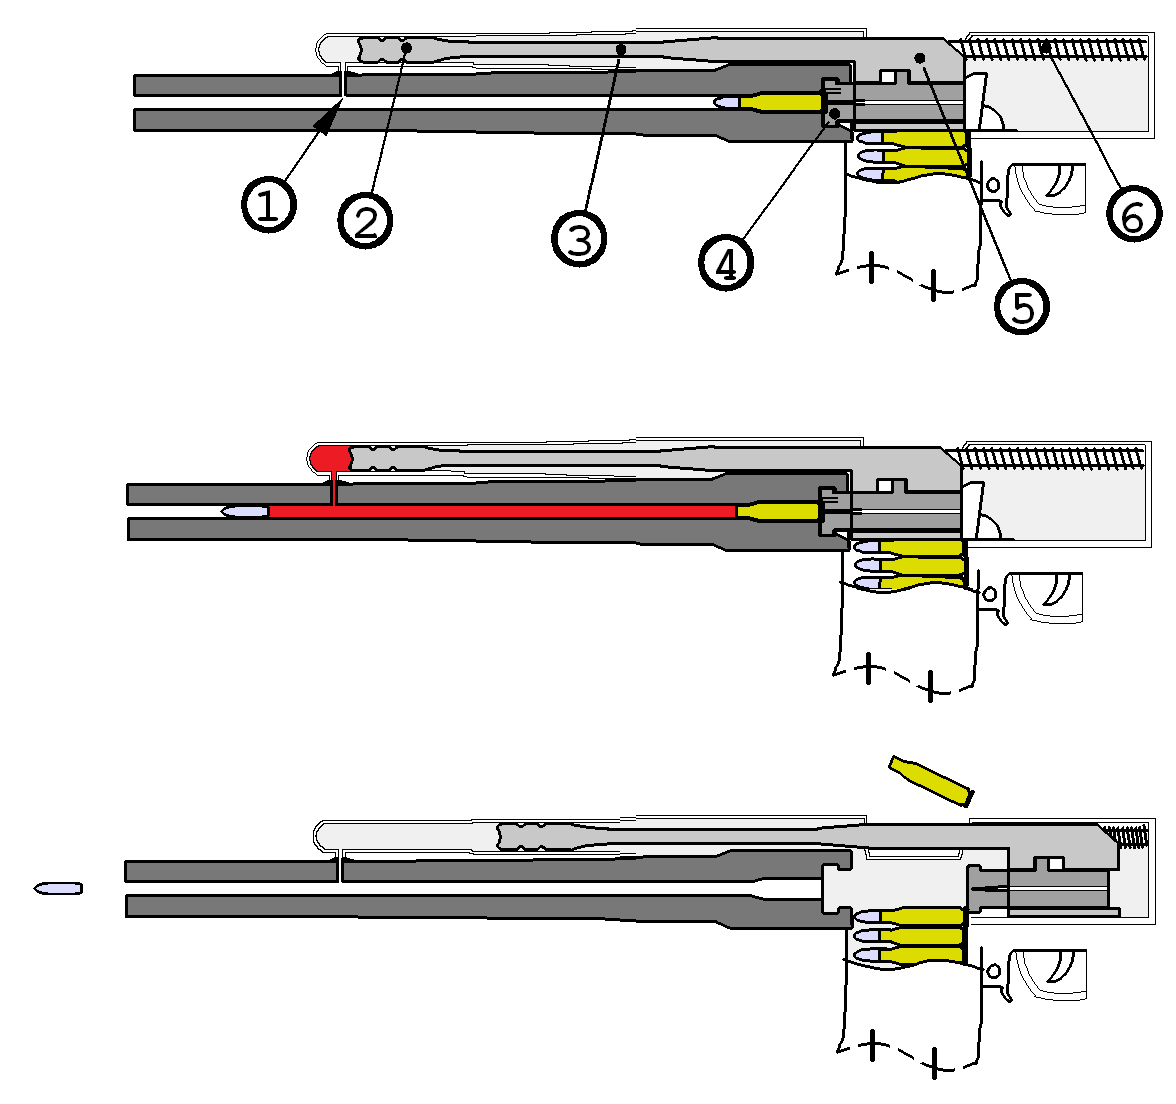
\includegraphics[width=0.65\textwidth]{image/abs_cd11_image1.png}
\end{center}
\figcaption{1}{Hệ thống trích khí trên súng tự nạp (Nguồn: Wikimedia Commons -- ``Gas-operated reloading'', CC BY-SA 4.0).}

Vị trí đặt lỗ trích quyết định trực tiếp tính toàn vẹn của vũ khí. Lỗ trích đặt quá gần buồng đốt sẽ phải hứng chịu mức áp suất cực đoan, tạo ra xung lực đập nát linh kiện cơ khí khi đạn chưa thoát khỏi nòng. Ngược lại, nếu dời lỗ về quá xa, khối lượng khí giãn nở tiêu tán nhanh, áp lực sụt giảm lập tức gây kẹt đạn do bệ khóa nòng thiếu đà lùi.

Nhóm nghiên cứu khoan lỗ trích tại bốn tọa độ dọc nòng, lần lượt cách buồng đốt 150\,mm, 200\,mm, 250\,mm và 300\,mm, rồi đo áp suất khí thuốc và lực đẩy pít-tông sinh ra tại từng vị trí. Kết quả cho thấy vùng vận hành tối ưu nằm trong khoảng 170--220\,mm cách buồng đốt; ngoài dải này, hệ thống hoặc chịu xung lực cực đoan hoặc thiếu đà lùi. Trạng thái chu trình nạp đạn phụ thuộc vào tương quan giữa lực đẩy pít-tông và lực cản tổng hợp của lò xo lùi cùng cụm khóa nòng.

\tablecaption{1}{So sánh đặc tính động lực học tại bốn tọa độ khoan lỗ trích khí.}
\vspace{2pt}
\renewcommand{\arraystretch}{1.35}
{\small
\begin{center}
\begin{tabular}{|>{\centering\arraybackslash}m{2.2cm}|>{\centering\arraybackslash}m{1.8cm}|>{\centering\arraybackslash}m{2.2cm}|>{\raggedright\arraybackslash}m{4.5cm}|}
\hline
\rowcolor{primaryBlue!12}
\textbf{Vị trí cách buồng đốt} & \textbf{Áp suất (MPa)} & \textbf{Lực đẩy pít-tông (N)} & \multicolumn{1}{c|}{\cellcolor{primaryBlue!12}\textbf{Trạng thái}} \\
\hline
150\,mm & 85,0 & 9\,200 & Nguy hiểm (Rạn nứt pít-tông) \\
\hline
200\,mm & 52,0 & 5\,600 & Hoàn chỉnh (Chu trình khép kín) \\
\hline
250\,mm & 35,0 & 3\,800 & Không đủ (Kẹt vỏ đạn) \\
\hline
300\,mm & 22,0 & 2\,400 & Không đủ (Bệ khóa nòng bất động) \\
\hline
\end{tabular}
\end{center}
}
\vspace{2pt}
{\small\textit{Ghi chú: Lực cản lò xo lùi và cụm khóa nòng = 4\,200\,N. Hành trình pít-tông $s = 0{,}05$\,m.}}

\hfill\textbf{Nguồn: Nguyễn Nghĩa Đô biên soạn}
\end{readingpassage}

% === Câu 1: Trắc nghiệm ===
\question[Trắc nghiệm]{Tọa độ cách buồng đốt 200\,mm tương ứng với trạng thái vận hành nào của súng tự động?}
\par\vspace{4pt}
\noindent\hangindent=2.2em\hangafter=1\choiceitem{A}{Rạn nứt pít-tông do xung lực cực đoan.}\par\vspace{4pt}
\noindent\hangindent=2.2em\hangafter=1\choiceitem{B}{Bệ khóa nòng bất động do tiêu tán khí.}\par\vspace{4pt}
\noindent\hangindent=2.2em\hangafter=1\choiceitem{C}{Chu trình nạp đạn khép kín hoàn chỉnh.}\par\vspace{4pt}
\noindent\hangindent=2.2em\hangafter=1\choiceitem{D}{Kẹt vỏ đạn do bệ khóa nòng thiếu đà lùi.}\par\vspace{4pt}

% === Câu 2: Trắc nghiệm ===
\question[Trắc nghiệm]{Lực đẩy pít-tông sinh ra tại tọa độ cách buồng đốt 300\,mm có độ lớn bằng bao nhiêu?}
\par\vspace{4pt}
\noindent\choiceitem{A}{3\,800\,N.}\hfill\choiceitem{B}{9\,200\,N.}\hfill\choiceitem{C}{5\,600\,N.}\hfill\choiceitem{D}{2\,400\,N.}

% === Câu 3: Trắc nghiệm ===
\question[Trắc nghiệm]{Nguyên nhân vật lý nào khiến việc thiết kế lỗ trích khí tại vị trí 250\,mm dẫn đến tình trạng kẹt vỏ đạn?}
\par\vspace{4pt}
\noindent\hangindent=2.2em\hangafter=1\choiceitem{A}{Xung lực đập nát linh kiện cơ khí ngăn cản quá trình trích xuất vỏ đạn cũ.}\par\vspace{4pt}
\noindent\hangindent=2.2em\hangafter=1\choiceitem{B}{Lực đẩy (3\,800\,N) sinh ra nhỏ hơn lực cản tổng hợp (4\,200\,N), khiến cụm cơ cấu thiếu đà lùi.}\par\vspace{4pt}
\noindent\hangindent=2.2em\hangafter=1\choiceitem{C}{Khối lượng khí giãn nở bị tiêu tán quá chậm khiến áp suất duy trì ở mức quá cao.}\par\vspace{4pt}
\noindent\hangindent=2.2em\hangafter=1\choiceitem{D}{Lực cản lò xo lùi tự sinh ra phản lực 4\,800\,N vượt qua lực đẩy.}\par\vspace{4pt}

% === Câu 4: Đúng/Sai ===
\question[Đúng/Sai]{Đánh giá các phát biểu sau về đặc tính động lực học tại các vị trí khoan lỗ trích khí:}

\vspace{6pt}
\renewcommand{\arraystretch}{1.4}
{\small\setstretch{1.0}
\begin{longtable}{|>{\raggedright\arraybackslash}m{0.72\textwidth}|>{\centering\arraybackslash}m{0.08\textwidth}|>{\centering\arraybackslash}m{0.08\textwidth}|}
\hline
\rowcolor{primaryBlue!12}
\textbf{Nội dung} & \textbf{Đúng} & \textbf{Sai} \\
\hline
\endfirsthead
\hline
\rowcolor{primaryBlue!12}
\textbf{Nội dung} & \textbf{Đúng} & \textbf{Sai} \\
\hline
\endhead
a) Vị trí 150\,mm sinh ra lực đẩy vượt quá 4\,200\,N nên đảm bảo chu trình nạp đạn diễn ra trơn tru. & \tfcircle & \tfcircle \\
\hline
b) Vị trí lỗ trích thực tế tại 190\,mm được định vị nằm gọn bên trong vùng vận hành tối ưu của vũ khí. & \tfcircle & \tfcircle \\
\hline
c) Khi dời lỗ trích khí về mốc 300\,mm, khí giãn nở tiêu tán nhiều khiến áp lực giảm sút, bệ khóa nòng hoàn toàn bất động. & \tfcircle & \tfcircle \\
\hline
d) Áp suất khí thuốc suy giảm theo tỉ lệ tuyến tính khi đầu đạn tiến dần về phía mũi nòng. & \tfcircle & \tfcircle \\
\hline
\end{longtable}
}

% === Câu 5: Trắc nghiệm ===
\question[Trắc nghiệm]{So sánh mức chênh lệch về ``dư lực'' (hiệu số giữa lực đẩy pít-tông và lực cản tổng hợp) tác dụng lên bệ khóa nòng giữa hai vị trí 150\,mm và 200\,mm. Mức chênh lệch dư lực này là bao nhiêu?}
\par\vspace{4pt}
\noindent\choiceitem{A}{3\,600\,N.}\hfill\choiceitem{B}{5\,000\,N.}\hfill\choiceitem{C}{1\,400\,N.}\hfill\choiceitem{D}{4\,200\,N.}

% === Câu 6: Trắc nghiệm ===
\question[Trắc nghiệm]{Hiệu suất cơ học của pít-tông tại tọa độ 200\,mm (tỉ số giữa công tối thiểu cần thiết để thắng lực cản và tổng công do pít-tông thực sự sinh ra) có giá trị bằng bao nhiêu?}
\par\vspace{4pt}
\noindent\choiceitem{A}{$46\%$.}\hfill\choiceitem{B}{$75\%$.}\hfill\choiceitem{C}{$68\%$.}\hfill\choiceitem{D}{$100\%$.}

% === Câu 7: Trắc nghiệm ===
\question[Trắc nghiệm]{Nếu nhóm nghiên cứu tiến hành rút ngắn $10\%$ hành trình lùi của pít-tông nhằm tăng tốc độ khai hỏa, trong khi vẫn cố định lỗ trích ở 200\,mm, tổng công cơ học do pít-tông sinh ra sẽ thay đổi như thế nào so với thiết kế ban đầu?}
\par\vspace{4pt}
\noindent\hangindent=2.2em\hangafter=1\choiceitem{A}{Giảm đi 14\,J.}\par\vspace{4pt}
\noindent\hangindent=2.2em\hangafter=1\choiceitem{B}{Giữ nguyên 280\,J.}\par\vspace{4pt}
\noindent\hangindent=2.2em\hangafter=1\choiceitem{C}{Tăng thêm 28\,J.}\par\vspace{4pt}
\noindent\hangindent=2.2em\hangafter=1\choiceitem{D}{Giảm đi 28\,J.}\par\vspace{4pt}

% === Câu 8: Trắc nghiệm ===
\question[Trắc nghiệm]{Một xe máy điện trang bị hệ thống phanh tái sinh cho phép kỹ sư hiệu chỉnh mức thu hồi năng lượng. Dữ liệu thử nghiệm cho thấy: ở mức thu hồi thấp (dòng nạp ngược dưới 2\,A), xe gần như trôi tự do và năng lượng thu về không đáng kể; ở mức thu hồi cao (dòng nạp ngược trên 12\,A), bánh sau bị khóa cứng gây trượt mất lái. Dựa vào logic ba vùng vận hành trong cơ chế trích khí, phát biểu nào sau đây đánh giá đúng nhất bài toán hiệu chỉnh phanh tái sinh?}
\par\vspace{4pt}
\noindent\hangindent=2.2em\hangafter=1\choiceitem{A}{Dòng nạp ngược 2\,A tương đương trạng thái tại vị trí 150\,mm vì cả hai đều sinh ra tác dụng nhỏ nhất trong hệ thống.}\par\vspace{4pt}
\noindent\hangindent=2.2em\hangafter=1\choiceitem{B}{Để tối đa năng lượng thu hồi, kỹ sư nên đặt mức dòng nạp ngược vượt 12\,A, tương đương việc khoan lỗ trích ở vùng 0--170\,mm để khai thác toàn bộ áp suất khí thuốc.}\par\vspace{4pt}
\noindent\hangindent=2.2em\hangafter=1\choiceitem{C}{Khoảng dòng nạp ngược tối ưu nằm giữa 2\,A và 12\,A, tương tự dải 170--220\,mm: đủ lực thu hồi năng lượng mà không gây mất ổn định cơ học cho xe.}\par\vspace{4pt}
\noindent\hangindent=2.2em\hangafter=1\choiceitem{D}{Bài toán hiệu chỉnh phanh tái sinh không thể ánh xạ sang cơ chế trích khí vì hai hệ thống sử dụng hai dạng năng lượng hoàn toàn khác nhau.}\par\vspace{4pt}

% === Câu 9: Trắc nghiệm ===
\question[Trắc nghiệm]{Kỹ sư phát hiện rằng trong điều kiện nhiệt độ cao (trên 45\textdegree{}C), lò xo lùi bị giãn nhiệt, làm lực cản tổng hợp giảm xuống còn 3\,500\,N. Với lỗ trích vẫn cố định tại 250\,mm, sự thay đổi điều kiện nhiệt độ này ảnh hưởng như thế nào đến trạng thái vận hành của súng?}
\par\vspace{4pt}
\noindent\hangindent=2.2em\hangafter=1\choiceitem{A}{Súng vẫn kẹt vỏ đạn vì lực đẩy tại 250\,mm không đủ thắng lực cản ban đầu 4\,200\,N.}\par\vspace{4pt}
\noindent\hangindent=2.2em\hangafter=1\choiceitem{B}{Súng chuyển sang trạng thái hoàn chỉnh vì lực đẩy 3\,800\,N nay vượt lực cản mới 3\,500\,N.}\par\vspace{4pt}
\noindent\hangindent=2.2em\hangafter=1\choiceitem{C}{Súng chuyển sang trạng thái nguy hiểm vì nhiệt độ cao khuếch đại xung lực tác động lên pít-tông.}\par\vspace{4pt}
\noindent\hangindent=2.2em\hangafter=1\choiceitem{D}{Pít-tông lùi quá mức do lực cản suy yếu, gây rạn nứt tương tự vùng 0--170\,mm.}\par\vspace{4pt}

% === Câu 10: Trắc nghiệm ===
\question[Trắc nghiệm]{Nhà sản xuất phát triển một biến thể súng mới trang bị cụm khóa nòng nặng hơn, đẩy tổng lực cản của hệ thống lên mức 5\,000\,N. Để duy trì mức ``dư lực đẩy'' đúng bằng chênh lệch giữa lực đẩy và lực cản của bản thiết kế chuẩn ở tọa độ 200\,mm, kỹ sư cần khoan lỗ trích mới sinh ra lực đẩy bao nhiêu và dời lỗ trích về hướng nào?}
\par\vspace{4pt}
\noindent\hangindent=2.2em\hangafter=1\choiceitem{A}{6\,400\,N; dời lỗ trích lại gần buồng đốt hơn.}\par\vspace{4pt}
\noindent\hangindent=2.2em\hangafter=1\choiceitem{B}{3\,600\,N; dời lỗ trích lại gần buồng đốt hơn.}\par\vspace{4pt}
\noindent\hangindent=2.2em\hangafter=1\choiceitem{C}{6\,400\,N; dời lỗ trích ra xa buồng đốt hơn.}\par\vspace{4pt}
\noindent\hangindent=2.2em\hangafter=1\choiceitem{D}{5\,000\,N; giữ nguyên vị trí lỗ trích tại 200\,mm.}\par\vspace{4pt}

% ╔════════════════════════════════════════════════════════════╗
% ║  TRANG CUỐI - THAM GIA NHÓM ZALO                          ║
% ╚════════════════════════════════════════════════════════════╝
\newpage
\thispagestyle{empty}
\begin{center}
\vspace*{\fill}
\begin{tikzpicture}
    \node[draw=primaryBlue, line width=1.4pt, fill=pastelBlue,
          rounded corners=18pt, inner sep=26pt] {
        \begin{minipage}{0.72\textwidth}
            \centering
            {\color{primaryBlue}\fontsize{22}{28}\selectfont\textbf{THAM GIA NHÓM HỌC TẬP P20 STUDY}}\\[8pt]
            {\color{secondaryBlue}\fontsize{13}{17}\selectfont Cập nhật đề thi, tài liệu và thảo luận cùng cộng đồng}\\[10pt]
            {\color{lightBlue}\rule{0.7\linewidth}{0.8pt}}\\[14pt]
            
\includegraphics[width=4.2cm]{image/QR_zalo_moi.jpg}\\[12pt]
            {\color{textDark}\fontsize{12}{15}\selectfont Quét mã QR hoặc nhấn vào link bên dưới để tham gia}\\[6pt]
            {\fontsize{13}{16}\selectfont\href{https://zalo.me/g/docspspuvv8guthgtnvp}{\color{secondaryBlue}\underline{https://zalo.me/g/docspspuvv8guthgtnvp}}}\\[14pt]
            {\color{secondaryBlue}\small Hotline: 0388.389.569 \ $\vert$ \ Email: cskh@p20study.vn}
        \end{minipage}
    };
\end{tikzpicture}
\vspace*{\fill}
\end{center}

\end{document}